\documentclass[12pt,a4paper,fleqn]{report}
\usepackage{amssymb}
\usepackage[greek,english]{babel}
\usepackage[latin1]{inputenc}
\usepackage[only,bigsqcap]{stmaryrd}
\usepackage{textcomp}
\usepackage{latexsym}
\usepackage{graphicx}
\let\intorig=\int  %iman.sty redefines \int
\usepackage{../iman,../extra,../isar,../proof}
\usepackage[nohyphen,strings]{../underscore}
\usepackage{../isabelle,../isabellesym}
\usepackage{../ttbox,,../rail,../railsetup}
\usepackage{supertabular}
\usepackage{style}
\usepackage{../pdfsetup}

\hyphenation{Isabelle}
\hyphenation{Isar}

\isadroptag{theory}
\title{\includegraphics[scale=0.5]{isabelle_isar} \\[4ex] The Isabelle/Isar Reference Manual}
\author{\emph{Makarius Wenzel} \\[3ex]
  With Contributions by
  Clemens Ballarin,
  Stefan Berghofer, \\
  Lucas Dixon,
  Florian Haftmann,
  Gerwin Klein, \\
  Alexander Krauss,
  Tobias Nipkow,
  David von Oheimb, \\
  Larry Paulson,
  and Sebastian Skalberg
}

\makeindex

\railterm{percent,ppercent,underscore,lbrace,rbrace,atsign}
\railterm{ident,longident,symident,var,textvar,typefree,typevar,nat,string,verbatim,keyword}
\railterm{name,nameref,text,type,term,prop,atom}

\railalias{ident}{\railtok{ident}}
\railalias{longident}{\railtok{longident}}
\railalias{symident}{\railtok{symident}}
\railalias{var}{\railtok{var}}
\railalias{textvar}{\railtok{textvar}}
\railalias{typefree}{\railtok{typefree}}
\railalias{typevar}{\railtok{typevar}}
\railalias{nat}{\railtok{nat}}
\railalias{string}{\railtok{string}}
\railalias{verbatim}{\railtok{verbatim}}
\railalias{keyword}{\railtok{keyword}}

\railalias{name}{\railqtok{name}}
\railalias{nameref}{\railqtok{nameref}}
\railalias{text}{\railqtok{text}}
\railalias{type}{\railqtok{type}}
\railalias{term}{\railqtok{term}}
\railalias{prop}{\railqtok{prop}}
\railalias{atom}{\railqtok{atom}}

\railalias{subseteq}{\isasymsubseteq}\railterm{subseteq}
\railalias{equiv}{\isasymequiv}\railterm{equiv}
\railalias{rightleftharpoons}{\isasymrightleftharpoons}\railterm{rightleftharpoons}
\railalias{rightharpoonup}{\isasymrightharpoonup}\railterm{rightharpoonup}
\railalias{leftharpoondown}{\isasymleftharpoondown}\railterm{leftharpoondown}
\railalias{verblbrace}{\texttt{\ttlbrace*}}\railterm{verblbrace}
\railalias{verbrbrace}{\texttt{*\ttrbrace}}\railterm{verbrbrace}


\chardef\charbackquote=`\`
\newcommand{\backquote}{\mbox{\tt\charbackquote}}


\begin{document}

\maketitle 

\pagenumbering{roman} \tableofcontents \clearfirst

\part{Basic Concepts}
%
\begin{isabellebody}%
\def\isabellecontext{Introduction}%
%
\isadelimtheory
%
\endisadelimtheory
%
\isatagtheory
\isacommand{theory}\isamarkupfalse%
\ Introduction\isanewline
\isakeyword{imports}\ Setup\isanewline
\isakeyword{begin}%
\endisatagtheory
{\isafoldtheory}%
%
\isadelimtheory
%
\endisadelimtheory
%
\isamarkupchapter{Code generation from \isa{Isabelle{\isacharslash}HOL} theories%
}
\isamarkuptrue%
%
\isamarkupsection{Introduction and Overview%
}
\isamarkuptrue%
%
\begin{isamarkuptext}%
This tutorial introduces a generic code generator for the
  \isa{Isabelle} system.
  Generic in the sense that the
  \qn{target language} for which code shall ultimately be
  generated is not fixed but may be an arbitrary state-of-the-art
  functional programming language (currently, the implementation
  supports \isa{SML} \cite{SML}, \isa{OCaml} \cite{OCaml} and \isa{Haskell}
  \cite{haskell-revised-report}).

  Conceptually the code generator framework is part
  of Isabelle's \hyperlink{theory.Pure}{\mbox{\isa{Pure}}} meta logic framework; the logic
  \hyperlink{theory.HOL}{\mbox{\isa{HOL}}} which is an extension of \hyperlink{theory.Pure}{\mbox{\isa{Pure}}}
  already comes with a reasonable framework setup and thus provides
  a good working horse for raising code-generation-driven
  applications.  So, we assume some familiarity and experience
  with the ingredients of the \hyperlink{theory.HOL}{\mbox{\isa{HOL}}} distribution theories.
  (see also \cite{isa-tutorial}).

  The code generator aims to be usable with no further ado
  in most cases while allowing for detailed customisation.
  This manifests in the structure of this tutorial: after a short
  conceptual introduction with an example (\secref{sec:intro}),
  we discuss the generic customisation facilities (\secref{sec:program}).
  A further section (\secref{sec:adaption}) is dedicated to the matter of
  \qn{adaption} to specific target language environments.  After some
  further issues (\secref{sec:further}) we conclude with an overview
  of some ML programming interfaces (\secref{sec:ml}).

  \begin{warn}
    Ultimately, the code generator which this tutorial deals with
    is supposed to replace the existing code generator
    by Stefan Berghofer \cite{Berghofer-Nipkow:2002}.
    So, for the moment, there are two distinct code generators
    in Isabelle.  In case of ambiguity, we will refer to the framework
    described here as \isa{generic\ code\ generator}, to the
    other as \isa{SML\ code\ generator}.
    Also note that while the framework itself is
    object-logic independent, only \hyperlink{theory.HOL}{\mbox{\isa{HOL}}} provides a reasonable
    framework setup.    
  \end{warn}%
\end{isamarkuptext}%
\isamarkuptrue%
%
\isamarkupsubsection{Code generation via shallow embedding \label{sec:intro}%
}
\isamarkuptrue%
%
\begin{isamarkuptext}%
The key concept for understanding \isa{Isabelle}'s code generation is
  \emph{shallow embedding}, i.e.~logical entities like constants, types and
  classes are identified with corresponding concepts in the target language.

  Inside \hyperlink{theory.HOL}{\mbox{\isa{HOL}}}, the \hyperlink{command.datatype}{\mbox{\isa{\isacommand{datatype}}}} and
  \hyperlink{command.definition}{\mbox{\isa{\isacommand{definition}}}}/\hyperlink{command.primrec}{\mbox{\isa{\isacommand{primrec}}}}/\hyperlink{command.fun}{\mbox{\isa{\isacommand{fun}}}} declarations form
  the core of a functional programming language.  The default code generator setup
  allows to turn those into functional programs immediately.
  This means that \qt{naive} code generation can proceed without further ado.
  For example, here a simple \qt{implementation} of amortised queues:%
\end{isamarkuptext}%
\isamarkuptrue%
%
\isadelimquoteme
%
\endisadelimquoteme
%
\isatagquoteme
\isacommand{datatype}\isamarkupfalse%
\ {\isacharprime}a\ queue\ {\isacharequal}\ Queue\ {\isachardoublequoteopen}{\isacharprime}a\ list{\isachardoublequoteclose}\ {\isachardoublequoteopen}{\isacharprime}a\ list{\isachardoublequoteclose}\isanewline
\isanewline
\isacommand{definition}\isamarkupfalse%
\ empty\ {\isacharcolon}{\isacharcolon}\ {\isachardoublequoteopen}{\isacharprime}a\ queue{\isachardoublequoteclose}\ \isakeyword{where}\isanewline
\ \ {\isachardoublequoteopen}empty\ {\isacharequal}\ Queue\ {\isacharbrackleft}{\isacharbrackright}\ {\isacharbrackleft}{\isacharbrackright}{\isachardoublequoteclose}\isanewline
\isanewline
\isacommand{primrec}\isamarkupfalse%
\ enqueue\ {\isacharcolon}{\isacharcolon}\ {\isachardoublequoteopen}{\isacharprime}a\ {\isasymRightarrow}\ {\isacharprime}a\ queue\ {\isasymRightarrow}\ {\isacharprime}a\ queue{\isachardoublequoteclose}\ \isakeyword{where}\isanewline
\ \ {\isachardoublequoteopen}enqueue\ x\ {\isacharparenleft}Queue\ xs\ ys{\isacharparenright}\ {\isacharequal}\ Queue\ {\isacharparenleft}x\ {\isacharhash}\ xs{\isacharparenright}\ ys{\isachardoublequoteclose}\isanewline
\isanewline
\isacommand{fun}\isamarkupfalse%
\ dequeue\ {\isacharcolon}{\isacharcolon}\ {\isachardoublequoteopen}{\isacharprime}a\ queue\ {\isasymRightarrow}\ {\isacharprime}a\ option\ {\isasymtimes}\ {\isacharprime}a\ queue{\isachardoublequoteclose}\ \isakeyword{where}\isanewline
\ \ \ \ {\isachardoublequoteopen}dequeue\ {\isacharparenleft}Queue\ {\isacharbrackleft}{\isacharbrackright}\ {\isacharbrackleft}{\isacharbrackright}{\isacharparenright}\ {\isacharequal}\ {\isacharparenleft}None{\isacharcomma}\ Queue\ {\isacharbrackleft}{\isacharbrackright}\ {\isacharbrackleft}{\isacharbrackright}{\isacharparenright}{\isachardoublequoteclose}\isanewline
\ \ {\isacharbar}\ {\isachardoublequoteopen}dequeue\ {\isacharparenleft}Queue\ xs\ {\isacharparenleft}y\ {\isacharhash}\ ys{\isacharparenright}{\isacharparenright}\ {\isacharequal}\ {\isacharparenleft}Some\ y{\isacharcomma}\ Queue\ xs\ ys{\isacharparenright}{\isachardoublequoteclose}\isanewline
\ \ {\isacharbar}\ {\isachardoublequoteopen}dequeue\ {\isacharparenleft}Queue\ xs\ {\isacharbrackleft}{\isacharbrackright}{\isacharparenright}\ {\isacharequal}\isanewline
\ \ \ \ \ \ {\isacharparenleft}case\ rev\ xs\ of\ y\ {\isacharhash}\ ys\ {\isasymRightarrow}\ {\isacharparenleft}Some\ y{\isacharcomma}\ Queue\ {\isacharbrackleft}{\isacharbrackright}\ ys{\isacharparenright}{\isacharparenright}{\isachardoublequoteclose}%
\endisatagquoteme
{\isafoldquoteme}%
%
\isadelimquoteme
%
\endisadelimquoteme
%
\begin{isamarkuptext}%
\noindent Then we can generate code e.g.~for \isa{SML} as follows:%
\end{isamarkuptext}%
\isamarkuptrue%
%
\isadelimquoteme
%
\endisadelimquoteme
%
\isatagquoteme
\isacommand{export{\isacharunderscore}code}\isamarkupfalse%
\ empty\ dequeue\ enqueue\ \isakeyword{in}\ SML\isanewline
\ \ \isakeyword{module{\isacharunderscore}name}\ Example\ \isakeyword{file}\ {\isachardoublequoteopen}examples{\isacharslash}example{\isachardot}ML{\isachardoublequoteclose}%
\endisatagquoteme
{\isafoldquoteme}%
%
\isadelimquoteme
%
\endisadelimquoteme
%
\begin{isamarkuptext}%
\noindent resulting in the following code:%
\end{isamarkuptext}%
\isamarkuptrue%
%
\isadelimquoteme
%
\endisadelimquoteme
%
\isatagquoteme
%
\begin{isamarkuptext}%
\isaverbatim%
\noindent%
\verb|structure Example = |\newline%
\verb|struct|\newline%
\newline%
\verb|fun foldl f a [] = a|\newline%
\verb|  |\verb,|,\verb| foldl f a (x :: xs) = foldl f (f a x) xs;|\newline%
\newline%
\verb|fun rev xs = foldl (fn xsa => fn x => x :: xsa) [] xs;|\newline%
\newline%
\verb|fun list_case f1 f2 (a :: lista) = f2 a lista|\newline%
\verb|  |\verb,|,\verb| list_case f1 f2 [] = f1;|\newline%
\newline%
\verb|datatype 'a queue = Queue of 'a list * 'a list;|\newline%
\newline%
\verb|val empty : 'a queue = Queue ([], []);|\newline%
\newline%
\verb|fun dequeue (Queue ([], [])) = (NONE, Queue ([], []))|\newline%
\verb|  |\verb,|,\verb| dequeue (Queue (xs, y :: ys)) = (SOME y, Queue (xs, ys))|\newline%
\verb|  |\verb,|,\verb| dequeue (Queue (v :: va, [])) =|\newline%
\verb|    let|\newline%
\verb|      val y :: ys = rev (v :: va);|\newline%
\verb|    in|\newline%
\verb|      (SOME y, Queue ([], ys))|\newline%
\verb|    end;|\newline%
\newline%
\verb|fun enqueue x (Queue (xs, ys)) = Queue (x :: xs, ys);|\newline%
\newline%
\verb|end; (*struct Example*)|%
\end{isamarkuptext}%
\isamarkuptrue%
%
\endisatagquoteme
{\isafoldquoteme}%
%
\isadelimquoteme
%
\endisadelimquoteme
%
\begin{isamarkuptext}%
\noindent The \hyperlink{command.export-code}{\mbox{\isa{\isacommand{export{\isacharunderscore}code}}}} command takes a space-separated list of
  constants for which code shall be generated;  anything else needed for those
  is added implicitly.  Then follows a target language identifier
  (\isa{SML}, \isa{OCaml} or \isa{Haskell}) and a freely chosen module name.
  A file name denotes the destination to store the generated code.  Note that
  the semantics of the destination depends on the target language:  for
  \isa{SML} and \isa{OCaml} it denotes a \emph{file}, for \isa{Haskell}
  it denotes a \emph{directory} where a file named as the module name
  (with extension \isa{{\isachardot}hs}) is written:%
\end{isamarkuptext}%
\isamarkuptrue%
%
\isadelimquoteme
%
\endisadelimquoteme
%
\isatagquoteme
\isacommand{export{\isacharunderscore}code}\isamarkupfalse%
\ empty\ dequeue\ enqueue\ \isakeyword{in}\ Haskell\isanewline
\ \ \isakeyword{module{\isacharunderscore}name}\ Example\ \isakeyword{file}\ {\isachardoublequoteopen}examples{\isacharslash}{\isachardoublequoteclose}%
\endisatagquoteme
{\isafoldquoteme}%
%
\isadelimquoteme
%
\endisadelimquoteme
%
\begin{isamarkuptext}%
\noindent This is how the corresponding code in \isa{Haskell} looks like:%
\end{isamarkuptext}%
\isamarkuptrue%
%
\isadelimquoteme
%
\endisadelimquoteme
%
\isatagquoteme
%
\begin{isamarkuptext}%
\isaverbatim%
\noindent%
\verb|module Example where {|\newline%
\newline%
\newline%
\verb|foldla :: forall a b. (a -> b -> a) -> a -> [b] -> a;|\newline%
\verb|foldla f a [] = a;|\newline%
\verb|foldla f a (x : xs) = foldla f (f a x) xs;|\newline%
\newline%
\verb|rev :: forall a. [a] -> [a];|\newline%
\verb|rev xs = foldla (\ xsa x -> x : xsa) [] xs;|\newline%
\newline%
\verb|list_case :: forall t a. t -> (a -> [a] -> t) -> [a] -> t;|\newline%
\verb|list_case f1 f2 (a : list) = f2 a list;|\newline%
\verb|list_case f1 f2 [] = f1;|\newline%
\newline%
\verb|data Queue a = Queue [a] [a];|\newline%
\newline%
\verb|empty :: forall a. Queue a;|\newline%
\verb|empty = Queue [] [];|\newline%
\newline%
\verb|dequeue :: forall a. Queue a -> (Maybe a, Queue a);|\newline%
\verb|dequeue (Queue [] []) = (Nothing, Queue [] []);|\newline%
\verb|dequeue (Queue xs (y : ys)) = (Just y, Queue xs ys);|\newline%
\verb|dequeue (Queue (v : va) []) =|\newline%
\verb|  let {|\newline%
\verb|    (y : ys) = rev (v : va);|\newline%
\verb|  } in (Just y, Queue [] ys);|\newline%
\newline%
\verb|enqueue :: forall a. a -> Queue a -> Queue a;|\newline%
\verb|enqueue x (Queue xs ys) = Queue (x : xs) ys;|\newline%
\newline%
\verb|}|%
\end{isamarkuptext}%
\isamarkuptrue%
%
\endisatagquoteme
{\isafoldquoteme}%
%
\isadelimquoteme
%
\endisadelimquoteme
%
\begin{isamarkuptext}%
\noindent This demonstrates the basic usage of the \hyperlink{command.export-code}{\mbox{\isa{\isacommand{export{\isacharunderscore}code}}}} command;
  for more details see \secref{sec:further}.%
\end{isamarkuptext}%
\isamarkuptrue%
%
\isamarkupsubsection{Code generator architecture \label{sec:concept}%
}
\isamarkuptrue%
%
\begin{isamarkuptext}%
What you have seen so far should be already enough in a lot of cases.  If you
  are content with this, you can quit reading here.  Anyway, in order to customise
  and adapt the code generator, it is inevitable to gain some understanding
  how it works.

  \begin{figure}[h]
    \centering
    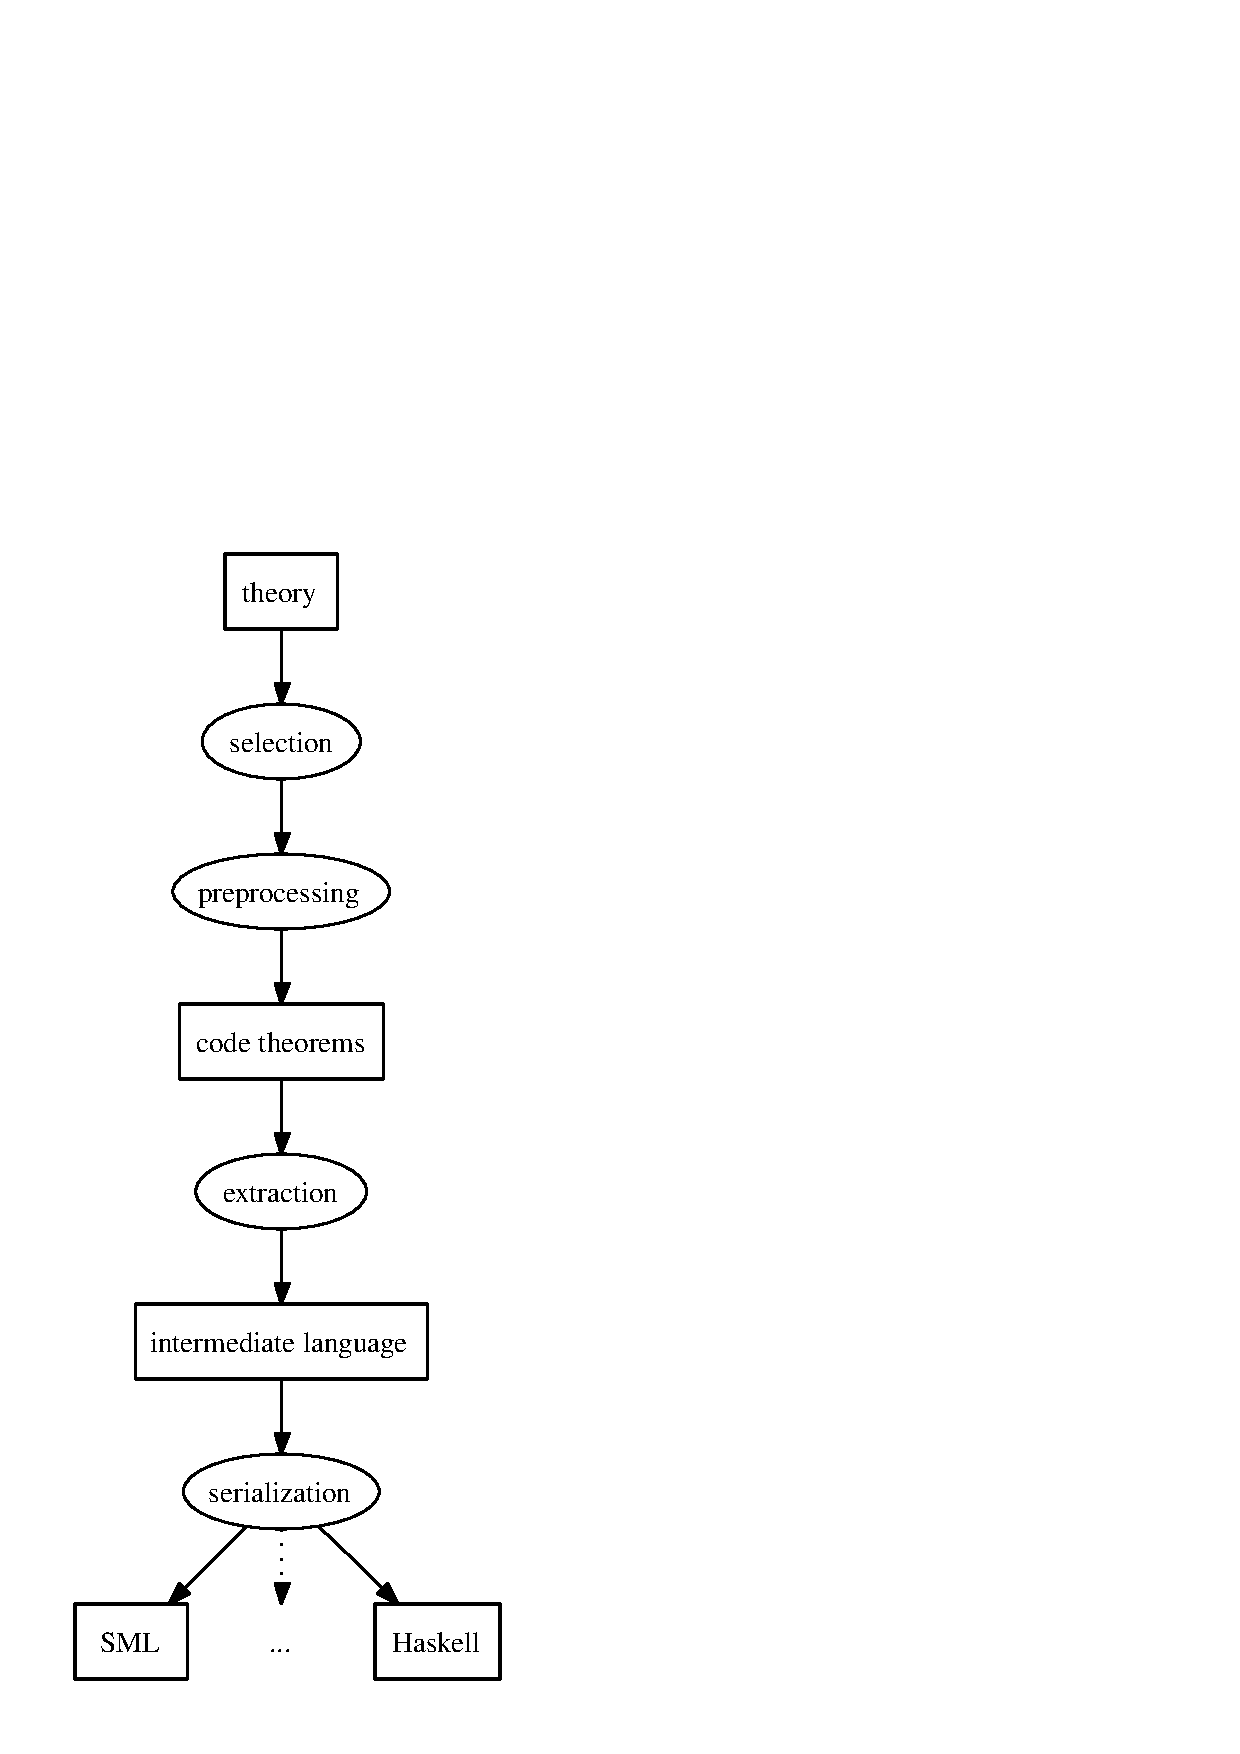
\includegraphics[width=0.7\textwidth]{codegen_process}
    \caption{Code generator architecture}
    \label{fig:arch}
  \end{figure}

  The code generator employs a notion of executability
  for three foundational executable ingredients known
  from functional programming:
  \emph{defining equations}, \emph{datatypes}, and
  \emph{type classes}.  A defining equation as a first approximation
  is a theorem of the form \isa{f\ t\isactrlisub {\isadigit{1}}\ t\isactrlisub {\isadigit{2}}\ {\isasymdots}\ t\isactrlisub n\ {\isasymequiv}\ t}
  (an equation headed by a constant \isa{f} with arguments
  \isa{t\isactrlisub {\isadigit{1}}\ t\isactrlisub {\isadigit{2}}\ {\isasymdots}\ t\isactrlisub n} and right hand side \isa{t}).
  Code generation aims to turn defining equations
  into a functional program.  This is achieved by three major
  components which operate sequentially, i.e. the result of one is
  the input
  of the next in the chain,  see diagram \ref{fig:arch}:

  \begin{itemize}

    \item Out of the vast collection of theorems proven in a
      \qn{theory}, a reasonable subset modelling
      defining equations is \qn{selected}.

    \item On those selected theorems, certain
      transformations are carried out
      (\qn{preprocessing}).  Their purpose is to turn theorems
      representing non- or badly executable
      specifications into equivalent but executable counterparts.
      The result is a structured collection of \qn{code theorems}.

    \item Before the selected defining equations are continued with,
      they can be \qn{preprocessed}, i.e. subjected to theorem
      transformations.  This \qn{preprocessor} is an interface which
      allows to apply
      the full expressiveness of ML-based theorem transformations
      to code generation;  motivating examples are shown below, see
      \secref{sec:preproc}.
      The result of the preprocessing step is a structured collection
      of defining equations.

    \item These defining equations are \qn{translated} to a program
      in an abstract intermediate language.  Think of it as a kind
      of \qt{Mini-Haskell} with four \qn{statements}: \isa{data}
      (for datatypes), \isa{fun} (stemming from defining equations),
      also \isa{class} and \isa{inst} (for type classes).

    \item Finally, the abstract program is \qn{serialised} into concrete
      source code of a target language.

  \end{itemize}

  \noindent From these steps, only the two last are carried out outside the logic;  by
  keeping this layer as thin as possible, the amount of code to trust is
  kept to a minimum.%
\end{isamarkuptext}%
\isamarkuptrue%
%
\isadelimtheory
%
\endisadelimtheory
%
\isatagtheory
\isacommand{end}\isamarkupfalse%
%
\endisatagtheory
{\isafoldtheory}%
%
\isadelimtheory
%
\endisadelimtheory
\isanewline
\end{isabellebody}%
%%% Local Variables:
%%% mode: latex
%%% TeX-master: "root"
%%% End:

%
\begin{isabellebody}%
\def\isabellecontext{Framework}%
%
\isadelimtheory
%
\endisadelimtheory
%
\isatagtheory
\isacommand{theory}\isamarkupfalse%
\ Framework\isanewline
\isakeyword{imports}\ Main\isanewline
\isakeyword{begin}%
\endisatagtheory
{\isafoldtheory}%
%
\isadelimtheory
%
\endisadelimtheory
%
\isamarkupchapter{The Isabelle/Isar Framework \label{ch:isar-framework}%
}
\isamarkuptrue%
%
\begin{isamarkuptext}%
Isabelle/Isar
  \cite{Wenzel:1999:TPHOL,Wenzel-PhD,Nipkow-TYPES02,Wenzel-Paulson:2006,Wenzel:2006:Festschrift}
  is intended as a generic framework for developing formal
  mathematical documents with full proof checking.  Definitions and
  proofs are organized as theories; an assembly of theory sources may
  be presented as a printed document; see also
  \chref{ch:document-prep}.

  The main objective of Isar is the design of a human-readable
  structured proof language, which is called the ``primary proof
  format'' in Isar terminology.  Such a primary proof language is
  somewhere in the middle between the extremes of primitive proof
  objects and actual natural language.  In this respect, Isar is a bit
  more formalistic than Mizar
  \cite{Trybulec:1993:MizarFeatures,Rudnicki:1992:MizarOverview,Wiedijk:1999:Mizar},
  using logical symbols for certain reasoning schemes where Mizar
  would prefer English words; see \cite{Wenzel-Wiedijk:2002} for
  further comparisons of these systems.

  So Isar challenges the traditional way of recording informal proofs
  in mathematical prose, as well as the common tendency to see fully
  formal proofs directly as objects of some logical calculus (e.g.\
  \isa{{\isachardoublequote}{\isasymlambda}{\isachardoublequote}}-terms in a version of type theory).  In fact, Isar is
  better understood as an interpreter of a simple block-structured
  language for describing data flow of local facts and goals,
  interspersed with occasional invocations of proof methods.
  Everything is reduced to logical inferences internally, but these
  steps are somewhat marginal compared to the overall bookkeeping of
  the interpretation process.  Thanks to careful design of the syntax
  and semantics of Isar language elements, a formal record of Isar
  instructions may later appear as an intelligible text to the
  attentive reader.

  The Isar proof language has emerged from careful analysis of some
  inherent virtues of the existing logical framework of Isabelle/Pure
  \cite{paulson-found,paulson700}, notably composition of higher-order
  natural deduction rules, which is a generalization of Gentzen's
  original calculus \cite{Gentzen:1935}.  The approach of generic
  inference systems in Pure is continued by Isar towards actual proof
  texts.

  Concrete applications require another intermediate layer: an
  object-logic.  Isabelle/HOL \cite{isa-tutorial} (simply-typed
  set-theory) is being used most of the time; Isabelle/ZF
  \cite{isabelle-ZF} is less extensively developed, although it would
  probably fit better for classical mathematics.

  \medskip In order to illustrate typical natural deduction reasoning
  in Isar, we shall refer to the background theory and library of
  Isabelle/HOL.  This includes common notions of predicate logic,
  naive set-theory etc.\ using fairly standard mathematical notation.
  From the perspective of generic natural deduction there is nothing
  special about the logical connectives of HOL (\isa{{\isachardoublequote}{\isasymand}{\isachardoublequote}}, \isa{{\isachardoublequote}{\isasymor}{\isachardoublequote}}, \isa{{\isachardoublequote}{\isasymforall}{\isachardoublequote}}, \isa{{\isachardoublequote}{\isasymexists}{\isachardoublequote}}, etc.), only the resulting reasoning
  principles are relevant to the user.  There are similar rules
  available for set-theory operators (\isa{{\isachardoublequote}{\isasyminter}{\isachardoublequote}}, \isa{{\isachardoublequote}{\isasymunion}{\isachardoublequote}}, \isa{{\isachardoublequote}{\isasymInter}{\isachardoublequote}}, \isa{{\isachardoublequote}{\isasymUnion}{\isachardoublequote}}, etc.), or any other theory developed in the
  library (lattice theory, topology etc.).

  Subsequently we briefly review fragments of Isar proof texts
  corresponding directly to such general natural deduction schemes.
  The examples shall refer to set-theory, to minimize the danger of
  understanding connectives of predicate logic as something special.

  \medskip The following deduction performs \isa{{\isachardoublequote}{\isasyminter}{\isachardoublequote}}-introduction,
  working forwards from assumptions towards the conclusion.  We give
  both the Isar text, and depict the primitive rule involved, as
  determined by unification of the problem against rules from the
  context.%
\end{isamarkuptext}%
\isamarkuptrue%
%
\medskip\begin{minipage}{0.6\textwidth}
%
\isadelimproof
%
\endisadelimproof
%
\isatagproof
\ \ \ \ \isacommand{assume}\isamarkupfalse%
\ {\isachardoublequoteopen}x\ {\isasymin}\ A{\isachardoublequoteclose}\ \isakeyword{and}\ {\isachardoublequoteopen}x\ {\isasymin}\ B{\isachardoublequoteclose}\isanewline
\ \ \ \ \isacommand{then}\isamarkupfalse%
\ \isacommand{have}\isamarkupfalse%
\ {\isachardoublequoteopen}x\ {\isasymin}\ A\ {\isasyminter}\ B{\isachardoublequoteclose}\ \isacommand{{\isachardot}{\isachardot}}\isamarkupfalse%
%
\endisatagproof
{\isafoldproof}%
%
\isadelimproof
%
\endisadelimproof
%
\end{minipage}\begin{minipage}{0.4\textwidth}
%
\begin{isamarkuptext}%
\infer{\isa{{\isachardoublequote}x\ {\isasymin}\ A\ {\isasyminter}\ B{\isachardoublequote}}}{\isa{{\isachardoublequote}x\ {\isasymin}\ A{\isachardoublequote}} & \isa{{\isachardoublequote}x\ {\isasymin}\ B{\isachardoublequote}}}%
\end{isamarkuptext}%
\isamarkuptrue%
%
\end{minipage}
%
\begin{isamarkuptext}%
\medskip\noindent Note that \hyperlink{command.assume}{\mbox{\isa{\isacommand{assume}}}} augments the
  context, \hyperlink{command.then}{\mbox{\isa{\isacommand{then}}}} indicates that the current facts shall be
  used in the next step, and \hyperlink{command.have}{\mbox{\isa{\isacommand{have}}}} states a local claim.
  The two dots ``\hyperlink{command.ddot}{\mbox{\isa{\isacommand{{\isachardot}{\isachardot}}}}}'' above refer to a complete proof of
  the claim, using the indicated facts and a canonical rule from the
  context.  We could have been more explicit here by spelling out the
  final proof step via the \hyperlink{command.by}{\mbox{\isa{\isacommand{by}}}} command:%
\end{isamarkuptext}%
\isamarkuptrue%
%
\isadelimproof
%
\endisadelimproof
%
\isatagproof
\ \ \ \ \isacommand{assume}\isamarkupfalse%
\ {\isachardoublequoteopen}x\ {\isasymin}\ A{\isachardoublequoteclose}\ \isakeyword{and}\ {\isachardoublequoteopen}x\ {\isasymin}\ B{\isachardoublequoteclose}\isanewline
\ \ \ \ \isacommand{then}\isamarkupfalse%
\ \isacommand{have}\isamarkupfalse%
\ {\isachardoublequoteopen}x\ {\isasymin}\ A\ {\isasyminter}\ B{\isachardoublequoteclose}\ \isacommand{by}\isamarkupfalse%
\ {\isacharparenleft}rule\ IntI{\isacharparenright}%
\endisatagproof
{\isafoldproof}%
%
\isadelimproof
%
\endisadelimproof
%
\begin{isamarkuptext}%
\noindent The format of the \isa{{\isachardoublequote}{\isasyminter}{\isachardoublequote}}-introduction rule represents
  the most basic inference, which proceeds from given premises to a
  conclusion, without any additional context involved.

  \medskip The next example performs backwards introduction on \isa{{\isachardoublequote}{\isasymInter}{\isasymA}{\isachardoublequote}}, the intersection of all sets within a given set.  This
  requires a nested proof of set membership within a local context of
  an arbitrary-but-fixed member of the collection:%
\end{isamarkuptext}%
\isamarkuptrue%
%
\medskip\begin{minipage}{0.6\textwidth}
%
\isadelimproof
%
\endisadelimproof
%
\isatagproof
\ \ \ \ \isacommand{have}\isamarkupfalse%
\ {\isachardoublequoteopen}x\ {\isasymin}\ {\isasymInter}{\isasymA}{\isachardoublequoteclose}\isanewline
\ \ \ \ \isacommand{proof}\isamarkupfalse%
\isanewline
\ \ \ \ \ \ \isacommand{fix}\isamarkupfalse%
\ A\isanewline
\ \ \ \ \ \ \isacommand{assume}\isamarkupfalse%
\ {\isachardoublequoteopen}A\ {\isasymin}\ {\isasymA}{\isachardoublequoteclose}\isanewline
\ \ \ \ \ \ \isacommand{show}\isamarkupfalse%
\ {\isachardoublequoteopen}x\ {\isasymin}\ A{\isachardoublequoteclose}\ \isacommand{sorry}\isamarkupfalse%
\isanewline
\ \ \ \ \isacommand{qed}\isamarkupfalse%
%
\endisatagproof
{\isafoldproof}%
%
\isadelimproof
%
\endisadelimproof
%
\end{minipage}\begin{minipage}{0.4\textwidth}
%
\begin{isamarkuptext}%
\infer{\isa{{\isachardoublequote}x\ {\isasymin}\ {\isasymInter}{\isasymA}{\isachardoublequote}}}{\infer*{\isa{{\isachardoublequote}x\ {\isasymin}\ A{\isachardoublequote}}}{\isa{{\isachardoublequote}{\isacharbrackleft}A{\isacharbrackright}{\isacharbrackleft}A\ {\isasymin}\ {\isasymA}{\isacharbrackright}{\isachardoublequote}}}}%
\end{isamarkuptext}%
\isamarkuptrue%
%
\end{minipage}
%
\begin{isamarkuptext}%
\medskip\noindent This Isar reasoning pattern again refers to the
  primitive rule depicted above.  The system determines it in the
  ``\hyperlink{command.proof}{\mbox{\isa{\isacommand{proof}}}}'' step, which could have been spelt out more
  explicitly as ``\hyperlink{command.proof}{\mbox{\isa{\isacommand{proof}}}}~\isa{{\isachardoublequote}{\isacharparenleft}{\isachardoublequote}}\hyperlink{method.rule}{\mbox{\isa{rule}}}~\hyperlink{fact.InterI}{\mbox{\isa{InterI}}}\isa{{\isachardoublequote}{\isacharparenright}{\isachardoublequote}}''.  Note that this rule involves both a local
  parameter \isa{{\isachardoublequote}A{\isachardoublequote}} and an assumption \isa{{\isachardoublequote}A\ {\isasymin}\ {\isasymA}{\isachardoublequote}} in the
  nested reasoning.  This kind of compound rule typically demands a
  genuine sub-proof in Isar, working backwards rather than forwards as
  seen before.  In the proof body we encounter the \hyperlink{command.fix}{\mbox{\isa{\isacommand{fix}}}}-\hyperlink{command.assume}{\mbox{\isa{\isacommand{assume}}}}-\hyperlink{command.show}{\mbox{\isa{\isacommand{show}}}} skeleton of nested
  sub-proofs that is typical for Isar.  The final \hyperlink{command.show}{\mbox{\isa{\isacommand{show}}}} is
  like \hyperlink{command.have}{\mbox{\isa{\isacommand{have}}}} followed by an additional refinement of the
  enclosing claim, using the rule derived from the proof body.  The
  \hyperlink{command.sorry}{\mbox{\isa{\isacommand{sorry}}}} command stands for a hole in the proof -- it may
  be understood as an excuse for not providing a proper proof yet.

  \medskip The next example involves \isa{{\isachardoublequote}{\isasymUnion}{\isasymA}{\isachardoublequote}}, which can be
  characterized as the set of all \isa{{\isachardoublequote}x{\isachardoublequote}} such that \isa{{\isachardoublequote}{\isasymexists}A{\isachardot}\ x\ {\isasymin}\ A\ {\isasymand}\ A\ {\isasymin}\ {\isasymA}{\isachardoublequote}}.  The elimination rule for \isa{{\isachardoublequote}x\ {\isasymin}\ {\isasymUnion}{\isasymA}{\isachardoublequote}} does
  not mention \isa{{\isachardoublequote}{\isasymexists}{\isachardoublequote}} and \isa{{\isachardoublequote}{\isasymand}{\isachardoublequote}} at all, but admits to obtain
  directly a local \isa{{\isachardoublequote}A{\isachardoublequote}} such that \isa{{\isachardoublequote}x\ {\isasymin}\ A{\isachardoublequote}} and \isa{{\isachardoublequote}A\ {\isasymin}\ {\isasymA}{\isachardoublequote}} hold.  This corresponds to the following Isar proof and
  inference rule, respectively:%
\end{isamarkuptext}%
\isamarkuptrue%
%
\medskip\begin{minipage}{0.6\textwidth}
%
\isadelimproof
%
\endisadelimproof
%
\isatagproof
\ \ \ \ \isacommand{assume}\isamarkupfalse%
\ {\isachardoublequoteopen}x\ {\isasymin}\ {\isasymUnion}{\isasymA}{\isachardoublequoteclose}\isanewline
\ \ \ \ \isacommand{then}\isamarkupfalse%
\ \isacommand{have}\isamarkupfalse%
\ C\isanewline
\ \ \ \ \isacommand{proof}\isamarkupfalse%
\isanewline
\ \ \ \ \ \ \isacommand{fix}\isamarkupfalse%
\ A\isanewline
\ \ \ \ \ \ \isacommand{assume}\isamarkupfalse%
\ {\isachardoublequoteopen}x\ {\isasymin}\ A{\isachardoublequoteclose}\ \isakeyword{and}\ {\isachardoublequoteopen}A\ {\isasymin}\ {\isasymA}{\isachardoublequoteclose}\isanewline
\ \ \ \ \ \ \isacommand{show}\isamarkupfalse%
\ C\ \isacommand{sorry}\isamarkupfalse%
\isanewline
\ \ \ \ \isacommand{qed}\isamarkupfalse%
%
\endisatagproof
{\isafoldproof}%
%
\isadelimproof
%
\endisadelimproof
%
\end{minipage}\begin{minipage}{0.4\textwidth}
%
\begin{isamarkuptext}%
\infer{\isa{{\isachardoublequote}C{\isachardoublequote}}}{\isa{{\isachardoublequote}x\ {\isasymin}\ {\isasymUnion}{\isasymA}{\isachardoublequote}} & \infer*{\isa{{\isachardoublequote}C{\isachardoublequote}}~}{\isa{{\isachardoublequote}{\isacharbrackleft}A{\isacharbrackright}{\isacharbrackleft}x\ {\isasymin}\ A{\isacharcomma}\ A\ {\isasymin}\ {\isasymA}{\isacharbrackright}{\isachardoublequote}}}}%
\end{isamarkuptext}%
\isamarkuptrue%
%
\end{minipage}
%
\begin{isamarkuptext}%
\medskip\noindent Although the Isar proof follows the natural
  deduction rule closely, the text reads not as natural as
  anticipated.  There is a double occurrence of an arbitrary
  conclusion \isa{{\isachardoublequote}C{\isachardoublequote}}, which represents the final result, but is
  irrelevant for now.  This issue arises for any elimination rule
  involving local parameters.  Isar provides the derived language
  element \hyperlink{command.obtain}{\mbox{\isa{\isacommand{obtain}}}}, which is able to perform the same
  elimination proof more conveniently:%
\end{isamarkuptext}%
\isamarkuptrue%
%
\isadelimproof
%
\endisadelimproof
%
\isatagproof
\ \ \ \ \isacommand{assume}\isamarkupfalse%
\ {\isachardoublequoteopen}x\ {\isasymin}\ {\isasymUnion}{\isasymA}{\isachardoublequoteclose}\isanewline
\ \ \ \ \isacommand{then}\isamarkupfalse%
\ \isacommand{obtain}\isamarkupfalse%
\ A\ \isakeyword{where}\ {\isachardoublequoteopen}x\ {\isasymin}\ A{\isachardoublequoteclose}\ \isakeyword{and}\ {\isachardoublequoteopen}A\ {\isasymin}\ {\isasymA}{\isachardoublequoteclose}\ \isacommand{{\isachardot}{\isachardot}}\isamarkupfalse%
%
\endisatagproof
{\isafoldproof}%
%
\isadelimproof
%
\endisadelimproof
%
\begin{isamarkuptext}%
\noindent Here we avoid to mention the final conclusion \isa{{\isachardoublequote}C{\isachardoublequote}}
  and return to plain forward reasoning.  The rule involved in the
  ``\hyperlink{command.ddot}{\mbox{\isa{\isacommand{{\isachardot}{\isachardot}}}}}'' proof is the same as before.%
\end{isamarkuptext}%
\isamarkuptrue%
%
\isadelimtheory
%
\endisadelimtheory
%
\isatagtheory
\isacommand{end}\isamarkupfalse%
%
\endisatagtheory
{\isafoldtheory}%
%
\isadelimtheory
%
\endisadelimtheory
\isanewline
\end{isabellebody}%
%%% Local Variables:
%%% mode: latex
%%% TeX-master: "root"
%%% End:

%
\begin{isabellebody}%
\def\isabellecontext{First{\isaliteral{5F}{\isacharunderscore}}Order{\isaliteral{5F}{\isacharunderscore}}Logic}%
%
\isamarkupheader{Example: First-Order Logic%
}
\isamarkuptrue%
%
\isadelimvisible
%
\endisadelimvisible
%
\isatagvisible
\isacommand{theory}\isamarkupfalse%
\ First{\isaliteral{5F}{\isacharunderscore}}Order{\isaliteral{5F}{\isacharunderscore}}Logic\isanewline
\isakeyword{imports}\ Base\ \ \isanewline
\isakeyword{begin}%
\endisatagvisible
{\isafoldvisible}%
%
\isadelimvisible
%
\endisadelimvisible
%
\begin{isamarkuptext}%
\noindent In order to commence a new object-logic within
  Isabelle/Pure we introduce abstract syntactic categories \isa{{\isaliteral{22}{\isachardoublequote}}i{\isaliteral{22}{\isachardoublequote}}}
  for individuals and \isa{{\isaliteral{22}{\isachardoublequote}}o{\isaliteral{22}{\isachardoublequote}}} for object-propositions.  The latter
  is embedded into the language of Pure propositions by means of a
  separate judgment.%
\end{isamarkuptext}%
\isamarkuptrue%
\isacommand{typedecl}\isamarkupfalse%
\ i\isanewline
\isacommand{typedecl}\isamarkupfalse%
\ o\isanewline
\isanewline
\isacommand{judgment}\isamarkupfalse%
\isanewline
\ \ Trueprop\ {\isaliteral{3A}{\isacharcolon}}{\isaliteral{3A}{\isacharcolon}}\ {\isaliteral{22}{\isachardoublequoteopen}}o\ {\isaliteral{5C3C52696768746172726F773E}{\isasymRightarrow}}\ prop{\isaliteral{22}{\isachardoublequoteclose}}\ \ \ \ {\isaliteral{28}{\isacharparenleft}}{\isaliteral{22}{\isachardoublequoteopen}}{\isaliteral{5F}{\isacharunderscore}}{\isaliteral{22}{\isachardoublequoteclose}}\ {\isadigit{5}}{\isaliteral{29}{\isacharparenright}}%
\begin{isamarkuptext}%
\noindent Note that the object-logic judgement is implicit in the
  syntax: writing \isa{A} produces \isa{{\isaliteral{22}{\isachardoublequote}}Trueprop\ A{\isaliteral{22}{\isachardoublequote}}} internally.
  From the Pure perspective this means ``\isa{A} is derivable in the
  object-logic''.%
\end{isamarkuptext}%
\isamarkuptrue%
%
\isamarkupsubsection{Equational reasoning \label{sec:framework-ex-equal}%
}
\isamarkuptrue%
%
\begin{isamarkuptext}%
Equality is axiomatized as a binary predicate on individuals, with
  reflexivity as introduction, and substitution as elimination
  principle.  Note that the latter is particularly convenient in a
  framework like Isabelle, because syntactic congruences are
  implicitly produced by unification of \isa{{\isaliteral{22}{\isachardoublequote}}B\ x{\isaliteral{22}{\isachardoublequote}}} against
  expressions containing occurrences of \isa{x}.%
\end{isamarkuptext}%
\isamarkuptrue%
\isacommand{axiomatization}\isamarkupfalse%
\isanewline
\ \ equal\ {\isaliteral{3A}{\isacharcolon}}{\isaliteral{3A}{\isacharcolon}}\ {\isaliteral{22}{\isachardoublequoteopen}}i\ {\isaliteral{5C3C52696768746172726F773E}{\isasymRightarrow}}\ i\ {\isaliteral{5C3C52696768746172726F773E}{\isasymRightarrow}}\ o{\isaliteral{22}{\isachardoublequoteclose}}\ \ {\isaliteral{28}{\isacharparenleft}}\isakeyword{infix}\ {\isaliteral{22}{\isachardoublequoteopen}}{\isaliteral{3D}{\isacharequal}}{\isaliteral{22}{\isachardoublequoteclose}}\ {\isadigit{5}}{\isadigit{0}}{\isaliteral{29}{\isacharparenright}}\isanewline
\isakeyword{where}\isanewline
\ \ refl\ {\isaliteral{5B}{\isacharbrackleft}}intro{\isaliteral{5D}{\isacharbrackright}}{\isaliteral{3A}{\isacharcolon}}\ {\isaliteral{22}{\isachardoublequoteopen}}x\ {\isaliteral{3D}{\isacharequal}}\ x{\isaliteral{22}{\isachardoublequoteclose}}\ \isakeyword{and}\isanewline
\ \ subst\ {\isaliteral{5B}{\isacharbrackleft}}elim{\isaliteral{5D}{\isacharbrackright}}{\isaliteral{3A}{\isacharcolon}}\ {\isaliteral{22}{\isachardoublequoteopen}}x\ {\isaliteral{3D}{\isacharequal}}\ y\ {\isaliteral{5C3C4C6F6E6772696768746172726F773E}{\isasymLongrightarrow}}\ B\ x\ {\isaliteral{5C3C4C6F6E6772696768746172726F773E}{\isasymLongrightarrow}}\ B\ y{\isaliteral{22}{\isachardoublequoteclose}}%
\begin{isamarkuptext}%
\noindent Substitution is very powerful, but also hard to control in
  full generality.  We derive some common symmetry~/ transitivity
  schemes of \isa{equal} as particular consequences.%
\end{isamarkuptext}%
\isamarkuptrue%
\isacommand{theorem}\isamarkupfalse%
\ sym\ {\isaliteral{5B}{\isacharbrackleft}}sym{\isaliteral{5D}{\isacharbrackright}}{\isaliteral{3A}{\isacharcolon}}\isanewline
\ \ \isakeyword{assumes}\ {\isaliteral{22}{\isachardoublequoteopen}}x\ {\isaliteral{3D}{\isacharequal}}\ y{\isaliteral{22}{\isachardoublequoteclose}}\isanewline
\ \ \isakeyword{shows}\ {\isaliteral{22}{\isachardoublequoteopen}}y\ {\isaliteral{3D}{\isacharequal}}\ x{\isaliteral{22}{\isachardoublequoteclose}}\isanewline
%
\isadelimproof
%
\endisadelimproof
%
\isatagproof
\isacommand{proof}\isamarkupfalse%
\ {\isaliteral{2D}{\isacharminus}}\isanewline
\ \ \isacommand{have}\isamarkupfalse%
\ {\isaliteral{22}{\isachardoublequoteopen}}x\ {\isaliteral{3D}{\isacharequal}}\ x{\isaliteral{22}{\isachardoublequoteclose}}\ \isacommand{{\isaliteral{2E}{\isachardot}}{\isaliteral{2E}{\isachardot}}}\isamarkupfalse%
\isanewline
\ \ \isacommand{with}\isamarkupfalse%
\ {\isaliteral{60}{\isacharbackquoteopen}}x\ {\isaliteral{3D}{\isacharequal}}\ y{\isaliteral{60}{\isacharbackquoteclose}}\ \isacommand{show}\isamarkupfalse%
\ {\isaliteral{22}{\isachardoublequoteopen}}y\ {\isaliteral{3D}{\isacharequal}}\ x{\isaliteral{22}{\isachardoublequoteclose}}\ \isacommand{{\isaliteral{2E}{\isachardot}}{\isaliteral{2E}{\isachardot}}}\isamarkupfalse%
\isanewline
\isacommand{qed}\isamarkupfalse%
%
\endisatagproof
{\isafoldproof}%
%
\isadelimproof
\isanewline
%
\endisadelimproof
\isanewline
\isacommand{theorem}\isamarkupfalse%
\ forw{\isaliteral{5F}{\isacharunderscore}}subst\ {\isaliteral{5B}{\isacharbrackleft}}trans{\isaliteral{5D}{\isacharbrackright}}{\isaliteral{3A}{\isacharcolon}}\isanewline
\ \ \isakeyword{assumes}\ {\isaliteral{22}{\isachardoublequoteopen}}y\ {\isaliteral{3D}{\isacharequal}}\ x{\isaliteral{22}{\isachardoublequoteclose}}\ \isakeyword{and}\ {\isaliteral{22}{\isachardoublequoteopen}}B\ x{\isaliteral{22}{\isachardoublequoteclose}}\isanewline
\ \ \isakeyword{shows}\ {\isaliteral{22}{\isachardoublequoteopen}}B\ y{\isaliteral{22}{\isachardoublequoteclose}}\isanewline
%
\isadelimproof
%
\endisadelimproof
%
\isatagproof
\isacommand{proof}\isamarkupfalse%
\ {\isaliteral{2D}{\isacharminus}}\isanewline
\ \ \isacommand{from}\isamarkupfalse%
\ {\isaliteral{60}{\isacharbackquoteopen}}y\ {\isaliteral{3D}{\isacharequal}}\ x{\isaliteral{60}{\isacharbackquoteclose}}\ \isacommand{have}\isamarkupfalse%
\ {\isaliteral{22}{\isachardoublequoteopen}}x\ {\isaliteral{3D}{\isacharequal}}\ y{\isaliteral{22}{\isachardoublequoteclose}}\ \isacommand{{\isaliteral{2E}{\isachardot}}{\isaliteral{2E}{\isachardot}}}\isamarkupfalse%
\isanewline
\ \ \isacommand{from}\isamarkupfalse%
\ this\ \isakeyword{and}\ {\isaliteral{60}{\isacharbackquoteopen}}B\ x{\isaliteral{60}{\isacharbackquoteclose}}\ \isacommand{show}\isamarkupfalse%
\ {\isaliteral{22}{\isachardoublequoteopen}}B\ y{\isaliteral{22}{\isachardoublequoteclose}}\ \isacommand{{\isaliteral{2E}{\isachardot}}{\isaliteral{2E}{\isachardot}}}\isamarkupfalse%
\isanewline
\isacommand{qed}\isamarkupfalse%
%
\endisatagproof
{\isafoldproof}%
%
\isadelimproof
\isanewline
%
\endisadelimproof
\isanewline
\isacommand{theorem}\isamarkupfalse%
\ back{\isaliteral{5F}{\isacharunderscore}}subst\ {\isaliteral{5B}{\isacharbrackleft}}trans{\isaliteral{5D}{\isacharbrackright}}{\isaliteral{3A}{\isacharcolon}}\isanewline
\ \ \isakeyword{assumes}\ {\isaliteral{22}{\isachardoublequoteopen}}B\ x{\isaliteral{22}{\isachardoublequoteclose}}\ \isakeyword{and}\ {\isaliteral{22}{\isachardoublequoteopen}}x\ {\isaliteral{3D}{\isacharequal}}\ y{\isaliteral{22}{\isachardoublequoteclose}}\isanewline
\ \ \isakeyword{shows}\ {\isaliteral{22}{\isachardoublequoteopen}}B\ y{\isaliteral{22}{\isachardoublequoteclose}}\isanewline
%
\isadelimproof
%
\endisadelimproof
%
\isatagproof
\isacommand{proof}\isamarkupfalse%
\ {\isaliteral{2D}{\isacharminus}}\isanewline
\ \ \isacommand{from}\isamarkupfalse%
\ {\isaliteral{60}{\isacharbackquoteopen}}x\ {\isaliteral{3D}{\isacharequal}}\ y{\isaliteral{60}{\isacharbackquoteclose}}\ \isakeyword{and}\ {\isaliteral{60}{\isacharbackquoteopen}}B\ x{\isaliteral{60}{\isacharbackquoteclose}}\isanewline
\ \ \isacommand{show}\isamarkupfalse%
\ {\isaliteral{22}{\isachardoublequoteopen}}B\ y{\isaliteral{22}{\isachardoublequoteclose}}\ \isacommand{{\isaliteral{2E}{\isachardot}}{\isaliteral{2E}{\isachardot}}}\isamarkupfalse%
\isanewline
\isacommand{qed}\isamarkupfalse%
%
\endisatagproof
{\isafoldproof}%
%
\isadelimproof
\isanewline
%
\endisadelimproof
\isanewline
\isacommand{theorem}\isamarkupfalse%
\ trans\ {\isaliteral{5B}{\isacharbrackleft}}trans{\isaliteral{5D}{\isacharbrackright}}{\isaliteral{3A}{\isacharcolon}}\isanewline
\ \ \isakeyword{assumes}\ {\isaliteral{22}{\isachardoublequoteopen}}x\ {\isaliteral{3D}{\isacharequal}}\ y{\isaliteral{22}{\isachardoublequoteclose}}\ \isakeyword{and}\ {\isaliteral{22}{\isachardoublequoteopen}}y\ {\isaliteral{3D}{\isacharequal}}\ z{\isaliteral{22}{\isachardoublequoteclose}}\isanewline
\ \ \isakeyword{shows}\ {\isaliteral{22}{\isachardoublequoteopen}}x\ {\isaliteral{3D}{\isacharequal}}\ z{\isaliteral{22}{\isachardoublequoteclose}}\isanewline
%
\isadelimproof
%
\endisadelimproof
%
\isatagproof
\isacommand{proof}\isamarkupfalse%
\ {\isaliteral{2D}{\isacharminus}}\isanewline
\ \ \isacommand{from}\isamarkupfalse%
\ {\isaliteral{60}{\isacharbackquoteopen}}y\ {\isaliteral{3D}{\isacharequal}}\ z{\isaliteral{60}{\isacharbackquoteclose}}\ \isakeyword{and}\ {\isaliteral{60}{\isacharbackquoteopen}}x\ {\isaliteral{3D}{\isacharequal}}\ y{\isaliteral{60}{\isacharbackquoteclose}}\isanewline
\ \ \isacommand{show}\isamarkupfalse%
\ {\isaliteral{22}{\isachardoublequoteopen}}x\ {\isaliteral{3D}{\isacharequal}}\ z{\isaliteral{22}{\isachardoublequoteclose}}\ \isacommand{{\isaliteral{2E}{\isachardot}}{\isaliteral{2E}{\isachardot}}}\isamarkupfalse%
\isanewline
\isacommand{qed}\isamarkupfalse%
%
\endisatagproof
{\isafoldproof}%
%
\isadelimproof
%
\endisadelimproof
%
\isamarkupsubsection{Basic group theory%
}
\isamarkuptrue%
%
\begin{isamarkuptext}%
As an example for equational reasoning we consider some bits of
  group theory.  The subsequent locale definition postulates group
  operations and axioms; we also derive some consequences of this
  specification.%
\end{isamarkuptext}%
\isamarkuptrue%
\isacommand{locale}\isamarkupfalse%
\ group\ {\isaliteral{3D}{\isacharequal}}\isanewline
\ \ \isakeyword{fixes}\ prod\ {\isaliteral{3A}{\isacharcolon}}{\isaliteral{3A}{\isacharcolon}}\ {\isaliteral{22}{\isachardoublequoteopen}}i\ {\isaliteral{5C3C52696768746172726F773E}{\isasymRightarrow}}\ i\ {\isaliteral{5C3C52696768746172726F773E}{\isasymRightarrow}}\ i{\isaliteral{22}{\isachardoublequoteclose}}\ \ {\isaliteral{28}{\isacharparenleft}}\isakeyword{infix}\ {\isaliteral{22}{\isachardoublequoteopen}}{\isaliteral{5C3C636972633E}{\isasymcirc}}{\isaliteral{22}{\isachardoublequoteclose}}\ {\isadigit{7}}{\isadigit{0}}{\isaliteral{29}{\isacharparenright}}\isanewline
\ \ \ \ \isakeyword{and}\ inv\ {\isaliteral{3A}{\isacharcolon}}{\isaliteral{3A}{\isacharcolon}}\ {\isaliteral{22}{\isachardoublequoteopen}}i\ {\isaliteral{5C3C52696768746172726F773E}{\isasymRightarrow}}\ i{\isaliteral{22}{\isachardoublequoteclose}}\ \ {\isaliteral{28}{\isacharparenleft}}{\isaliteral{22}{\isachardoublequoteopen}}{\isaliteral{28}{\isacharparenleft}}{\isaliteral{5F}{\isacharunderscore}}{\isaliteral{5C3C696E76657273653E}{\isasyminverse}}{\isaliteral{29}{\isacharparenright}}{\isaliteral{22}{\isachardoublequoteclose}}\ {\isaliteral{5B}{\isacharbrackleft}}{\isadigit{1}}{\isadigit{0}}{\isadigit{0}}{\isadigit{0}}{\isaliteral{5D}{\isacharbrackright}}\ {\isadigit{9}}{\isadigit{9}}{\isadigit{9}}{\isaliteral{29}{\isacharparenright}}\isanewline
\ \ \ \ \isakeyword{and}\ unit\ {\isaliteral{3A}{\isacharcolon}}{\isaliteral{3A}{\isacharcolon}}\ i\ \ {\isaliteral{28}{\isacharparenleft}}{\isaliteral{22}{\isachardoublequoteopen}}{\isadigit{1}}{\isaliteral{22}{\isachardoublequoteclose}}{\isaliteral{29}{\isacharparenright}}\isanewline
\ \ \isakeyword{assumes}\ assoc{\isaliteral{3A}{\isacharcolon}}\ {\isaliteral{22}{\isachardoublequoteopen}}{\isaliteral{28}{\isacharparenleft}}x\ {\isaliteral{5C3C636972633E}{\isasymcirc}}\ y{\isaliteral{29}{\isacharparenright}}\ {\isaliteral{5C3C636972633E}{\isasymcirc}}\ z\ {\isaliteral{3D}{\isacharequal}}\ x\ {\isaliteral{5C3C636972633E}{\isasymcirc}}\ {\isaliteral{28}{\isacharparenleft}}y\ {\isaliteral{5C3C636972633E}{\isasymcirc}}\ z{\isaliteral{29}{\isacharparenright}}{\isaliteral{22}{\isachardoublequoteclose}}\isanewline
\ \ \ \ \isakeyword{and}\ left{\isaliteral{5F}{\isacharunderscore}}unit{\isaliteral{3A}{\isacharcolon}}\ \ {\isaliteral{22}{\isachardoublequoteopen}}{\isadigit{1}}\ {\isaliteral{5C3C636972633E}{\isasymcirc}}\ x\ {\isaliteral{3D}{\isacharequal}}\ x{\isaliteral{22}{\isachardoublequoteclose}}\isanewline
\ \ \ \ \isakeyword{and}\ left{\isaliteral{5F}{\isacharunderscore}}inv{\isaliteral{3A}{\isacharcolon}}\ {\isaliteral{22}{\isachardoublequoteopen}}x{\isaliteral{5C3C696E76657273653E}{\isasyminverse}}\ {\isaliteral{5C3C636972633E}{\isasymcirc}}\ x\ {\isaliteral{3D}{\isacharequal}}\ {\isadigit{1}}{\isaliteral{22}{\isachardoublequoteclose}}\isanewline
\isakeyword{begin}\isanewline
\isanewline
\isacommand{theorem}\isamarkupfalse%
\ right{\isaliteral{5F}{\isacharunderscore}}inv{\isaliteral{3A}{\isacharcolon}}\ {\isaliteral{22}{\isachardoublequoteopen}}x\ {\isaliteral{5C3C636972633E}{\isasymcirc}}\ x{\isaliteral{5C3C696E76657273653E}{\isasyminverse}}\ {\isaliteral{3D}{\isacharequal}}\ {\isadigit{1}}{\isaliteral{22}{\isachardoublequoteclose}}\isanewline
%
\isadelimproof
%
\endisadelimproof
%
\isatagproof
\isacommand{proof}\isamarkupfalse%
\ {\isaliteral{2D}{\isacharminus}}\isanewline
\ \ \isacommand{have}\isamarkupfalse%
\ {\isaliteral{22}{\isachardoublequoteopen}}x\ {\isaliteral{5C3C636972633E}{\isasymcirc}}\ x{\isaliteral{5C3C696E76657273653E}{\isasyminverse}}\ {\isaliteral{3D}{\isacharequal}}\ {\isadigit{1}}\ {\isaliteral{5C3C636972633E}{\isasymcirc}}\ {\isaliteral{28}{\isacharparenleft}}x\ {\isaliteral{5C3C636972633E}{\isasymcirc}}\ x{\isaliteral{5C3C696E76657273653E}{\isasyminverse}}{\isaliteral{29}{\isacharparenright}}{\isaliteral{22}{\isachardoublequoteclose}}\ \isacommand{by}\isamarkupfalse%
\ {\isaliteral{28}{\isacharparenleft}}rule\ left{\isaliteral{5F}{\isacharunderscore}}unit\ {\isaliteral{5B}{\isacharbrackleft}}symmetric{\isaliteral{5D}{\isacharbrackright}}{\isaliteral{29}{\isacharparenright}}\isanewline
\ \ \isacommand{also}\isamarkupfalse%
\ \isacommand{have}\isamarkupfalse%
\ {\isaliteral{22}{\isachardoublequoteopen}}{\isaliteral{5C3C646F74733E}{\isasymdots}}\ {\isaliteral{3D}{\isacharequal}}\ {\isaliteral{28}{\isacharparenleft}}{\isadigit{1}}\ {\isaliteral{5C3C636972633E}{\isasymcirc}}\ x{\isaliteral{29}{\isacharparenright}}\ {\isaliteral{5C3C636972633E}{\isasymcirc}}\ x{\isaliteral{5C3C696E76657273653E}{\isasyminverse}}{\isaliteral{22}{\isachardoublequoteclose}}\ \isacommand{by}\isamarkupfalse%
\ {\isaliteral{28}{\isacharparenleft}}rule\ assoc\ {\isaliteral{5B}{\isacharbrackleft}}symmetric{\isaliteral{5D}{\isacharbrackright}}{\isaliteral{29}{\isacharparenright}}\isanewline
\ \ \isacommand{also}\isamarkupfalse%
\ \isacommand{have}\isamarkupfalse%
\ {\isaliteral{22}{\isachardoublequoteopen}}{\isadigit{1}}\ {\isaliteral{3D}{\isacharequal}}\ {\isaliteral{28}{\isacharparenleft}}x{\isaliteral{5C3C696E76657273653E}{\isasyminverse}}{\isaliteral{29}{\isacharparenright}}{\isaliteral{5C3C696E76657273653E}{\isasyminverse}}\ {\isaliteral{5C3C636972633E}{\isasymcirc}}\ x{\isaliteral{5C3C696E76657273653E}{\isasyminverse}}{\isaliteral{22}{\isachardoublequoteclose}}\ \isacommand{by}\isamarkupfalse%
\ {\isaliteral{28}{\isacharparenleft}}rule\ left{\isaliteral{5F}{\isacharunderscore}}inv\ {\isaliteral{5B}{\isacharbrackleft}}symmetric{\isaliteral{5D}{\isacharbrackright}}{\isaliteral{29}{\isacharparenright}}\isanewline
\ \ \isacommand{also}\isamarkupfalse%
\ \isacommand{have}\isamarkupfalse%
\ {\isaliteral{22}{\isachardoublequoteopen}}{\isaliteral{5C3C646F74733E}{\isasymdots}}\ {\isaliteral{5C3C636972633E}{\isasymcirc}}\ x\ {\isaliteral{3D}{\isacharequal}}\ {\isaliteral{28}{\isacharparenleft}}x{\isaliteral{5C3C696E76657273653E}{\isasyminverse}}{\isaliteral{29}{\isacharparenright}}{\isaliteral{5C3C696E76657273653E}{\isasyminverse}}\ {\isaliteral{5C3C636972633E}{\isasymcirc}}\ {\isaliteral{28}{\isacharparenleft}}x{\isaliteral{5C3C696E76657273653E}{\isasyminverse}}\ {\isaliteral{5C3C636972633E}{\isasymcirc}}\ x{\isaliteral{29}{\isacharparenright}}{\isaliteral{22}{\isachardoublequoteclose}}\ \isacommand{by}\isamarkupfalse%
\ {\isaliteral{28}{\isacharparenleft}}rule\ assoc{\isaliteral{29}{\isacharparenright}}\isanewline
\ \ \isacommand{also}\isamarkupfalse%
\ \isacommand{have}\isamarkupfalse%
\ {\isaliteral{22}{\isachardoublequoteopen}}x{\isaliteral{5C3C696E76657273653E}{\isasyminverse}}\ {\isaliteral{5C3C636972633E}{\isasymcirc}}\ x\ {\isaliteral{3D}{\isacharequal}}\ {\isadigit{1}}{\isaliteral{22}{\isachardoublequoteclose}}\ \isacommand{by}\isamarkupfalse%
\ {\isaliteral{28}{\isacharparenleft}}rule\ left{\isaliteral{5F}{\isacharunderscore}}inv{\isaliteral{29}{\isacharparenright}}\isanewline
\ \ \isacommand{also}\isamarkupfalse%
\ \isacommand{have}\isamarkupfalse%
\ {\isaliteral{22}{\isachardoublequoteopen}}{\isaliteral{28}{\isacharparenleft}}{\isaliteral{28}{\isacharparenleft}}x{\isaliteral{5C3C696E76657273653E}{\isasyminverse}}{\isaliteral{29}{\isacharparenright}}{\isaliteral{5C3C696E76657273653E}{\isasyminverse}}\ {\isaliteral{5C3C636972633E}{\isasymcirc}}\ {\isaliteral{5C3C646F74733E}{\isasymdots}}{\isaliteral{29}{\isacharparenright}}\ {\isaliteral{5C3C636972633E}{\isasymcirc}}\ x{\isaliteral{5C3C696E76657273653E}{\isasyminverse}}\ {\isaliteral{3D}{\isacharequal}}\ {\isaliteral{28}{\isacharparenleft}}x{\isaliteral{5C3C696E76657273653E}{\isasyminverse}}{\isaliteral{29}{\isacharparenright}}{\isaliteral{5C3C696E76657273653E}{\isasyminverse}}\ {\isaliteral{5C3C636972633E}{\isasymcirc}}\ {\isaliteral{28}{\isacharparenleft}}{\isadigit{1}}\ {\isaliteral{5C3C636972633E}{\isasymcirc}}\ x{\isaliteral{5C3C696E76657273653E}{\isasyminverse}}{\isaliteral{29}{\isacharparenright}}{\isaliteral{22}{\isachardoublequoteclose}}\ \isacommand{by}\isamarkupfalse%
\ {\isaliteral{28}{\isacharparenleft}}rule\ assoc{\isaliteral{29}{\isacharparenright}}\isanewline
\ \ \isacommand{also}\isamarkupfalse%
\ \isacommand{have}\isamarkupfalse%
\ {\isaliteral{22}{\isachardoublequoteopen}}{\isadigit{1}}\ {\isaliteral{5C3C636972633E}{\isasymcirc}}\ x{\isaliteral{5C3C696E76657273653E}{\isasyminverse}}\ {\isaliteral{3D}{\isacharequal}}\ x{\isaliteral{5C3C696E76657273653E}{\isasyminverse}}{\isaliteral{22}{\isachardoublequoteclose}}\ \isacommand{by}\isamarkupfalse%
\ {\isaliteral{28}{\isacharparenleft}}rule\ left{\isaliteral{5F}{\isacharunderscore}}unit{\isaliteral{29}{\isacharparenright}}\isanewline
\ \ \isacommand{also}\isamarkupfalse%
\ \isacommand{have}\isamarkupfalse%
\ {\isaliteral{22}{\isachardoublequoteopen}}{\isaliteral{28}{\isacharparenleft}}x{\isaliteral{5C3C696E76657273653E}{\isasyminverse}}{\isaliteral{29}{\isacharparenright}}{\isaliteral{5C3C696E76657273653E}{\isasyminverse}}\ {\isaliteral{5C3C636972633E}{\isasymcirc}}\ {\isaliteral{5C3C646F74733E}{\isasymdots}}\ {\isaliteral{3D}{\isacharequal}}\ {\isadigit{1}}{\isaliteral{22}{\isachardoublequoteclose}}\ \isacommand{by}\isamarkupfalse%
\ {\isaliteral{28}{\isacharparenleft}}rule\ left{\isaliteral{5F}{\isacharunderscore}}inv{\isaliteral{29}{\isacharparenright}}\isanewline
\ \ \isacommand{finally}\isamarkupfalse%
\ \isacommand{show}\isamarkupfalse%
\ {\isaliteral{22}{\isachardoublequoteopen}}x\ {\isaliteral{5C3C636972633E}{\isasymcirc}}\ x{\isaliteral{5C3C696E76657273653E}{\isasyminverse}}\ {\isaliteral{3D}{\isacharequal}}\ {\isadigit{1}}{\isaliteral{22}{\isachardoublequoteclose}}\ \isacommand{{\isaliteral{2E}{\isachardot}}}\isamarkupfalse%
\isanewline
\isacommand{qed}\isamarkupfalse%
%
\endisatagproof
{\isafoldproof}%
%
\isadelimproof
\isanewline
%
\endisadelimproof
\isanewline
\isacommand{theorem}\isamarkupfalse%
\ right{\isaliteral{5F}{\isacharunderscore}}unit{\isaliteral{3A}{\isacharcolon}}\ {\isaliteral{22}{\isachardoublequoteopen}}x\ {\isaliteral{5C3C636972633E}{\isasymcirc}}\ {\isadigit{1}}\ {\isaliteral{3D}{\isacharequal}}\ x{\isaliteral{22}{\isachardoublequoteclose}}\isanewline
%
\isadelimproof
%
\endisadelimproof
%
\isatagproof
\isacommand{proof}\isamarkupfalse%
\ {\isaliteral{2D}{\isacharminus}}\isanewline
\ \ \isacommand{have}\isamarkupfalse%
\ {\isaliteral{22}{\isachardoublequoteopen}}{\isadigit{1}}\ {\isaliteral{3D}{\isacharequal}}\ x{\isaliteral{5C3C696E76657273653E}{\isasyminverse}}\ {\isaliteral{5C3C636972633E}{\isasymcirc}}\ x{\isaliteral{22}{\isachardoublequoteclose}}\ \isacommand{by}\isamarkupfalse%
\ {\isaliteral{28}{\isacharparenleft}}rule\ left{\isaliteral{5F}{\isacharunderscore}}inv\ {\isaliteral{5B}{\isacharbrackleft}}symmetric{\isaliteral{5D}{\isacharbrackright}}{\isaliteral{29}{\isacharparenright}}\isanewline
\ \ \isacommand{also}\isamarkupfalse%
\ \isacommand{have}\isamarkupfalse%
\ {\isaliteral{22}{\isachardoublequoteopen}}x\ {\isaliteral{5C3C636972633E}{\isasymcirc}}\ {\isaliteral{5C3C646F74733E}{\isasymdots}}\ {\isaliteral{3D}{\isacharequal}}\ {\isaliteral{28}{\isacharparenleft}}x\ {\isaliteral{5C3C636972633E}{\isasymcirc}}\ x{\isaliteral{5C3C696E76657273653E}{\isasyminverse}}{\isaliteral{29}{\isacharparenright}}\ {\isaliteral{5C3C636972633E}{\isasymcirc}}\ x{\isaliteral{22}{\isachardoublequoteclose}}\ \isacommand{by}\isamarkupfalse%
\ {\isaliteral{28}{\isacharparenleft}}rule\ assoc\ {\isaliteral{5B}{\isacharbrackleft}}symmetric{\isaliteral{5D}{\isacharbrackright}}{\isaliteral{29}{\isacharparenright}}\isanewline
\ \ \isacommand{also}\isamarkupfalse%
\ \isacommand{have}\isamarkupfalse%
\ {\isaliteral{22}{\isachardoublequoteopen}}x\ {\isaliteral{5C3C636972633E}{\isasymcirc}}\ x{\isaliteral{5C3C696E76657273653E}{\isasyminverse}}\ {\isaliteral{3D}{\isacharequal}}\ {\isadigit{1}}{\isaliteral{22}{\isachardoublequoteclose}}\ \isacommand{by}\isamarkupfalse%
\ {\isaliteral{28}{\isacharparenleft}}rule\ right{\isaliteral{5F}{\isacharunderscore}}inv{\isaliteral{29}{\isacharparenright}}\isanewline
\ \ \isacommand{also}\isamarkupfalse%
\ \isacommand{have}\isamarkupfalse%
\ {\isaliteral{22}{\isachardoublequoteopen}}{\isaliteral{5C3C646F74733E}{\isasymdots}}\ {\isaliteral{5C3C636972633E}{\isasymcirc}}\ x\ {\isaliteral{3D}{\isacharequal}}\ x{\isaliteral{22}{\isachardoublequoteclose}}\ \isacommand{by}\isamarkupfalse%
\ {\isaliteral{28}{\isacharparenleft}}rule\ left{\isaliteral{5F}{\isacharunderscore}}unit{\isaliteral{29}{\isacharparenright}}\isanewline
\ \ \isacommand{finally}\isamarkupfalse%
\ \isacommand{show}\isamarkupfalse%
\ {\isaliteral{22}{\isachardoublequoteopen}}x\ {\isaliteral{5C3C636972633E}{\isasymcirc}}\ {\isadigit{1}}\ {\isaliteral{3D}{\isacharequal}}\ x{\isaliteral{22}{\isachardoublequoteclose}}\ \isacommand{{\isaliteral{2E}{\isachardot}}}\isamarkupfalse%
\isanewline
\isacommand{qed}\isamarkupfalse%
%
\endisatagproof
{\isafoldproof}%
%
\isadelimproof
%
\endisadelimproof
%
\begin{isamarkuptext}%
\noindent Reasoning from basic axioms is often tedious.  Our proofs
  work by producing various instances of the given rules (potentially
  the symmetric form) using the pattern ``\hyperlink{command.have}{\mbox{\isa{\isacommand{have}}}}~\isa{eq}~\hyperlink{command.by}{\mbox{\isa{\isacommand{by}}}}~\isa{{\isaliteral{22}{\isachardoublequote}}{\isaliteral{28}{\isacharparenleft}}rule\ r{\isaliteral{29}{\isacharparenright}}{\isaliteral{22}{\isachardoublequote}}}'' and composing the chain of
  results via \hyperlink{command.also}{\mbox{\isa{\isacommand{also}}}}/\hyperlink{command.finally}{\mbox{\isa{\isacommand{finally}}}}.  These steps may
  involve any of the transitivity rules declared in
  \secref{sec:framework-ex-equal}, namely \isa{trans} in combining
  the first two results in \isa{right{\isaliteral{5F}{\isacharunderscore}}inv} and in the final steps of
  both proofs, \isa{forw{\isaliteral{5F}{\isacharunderscore}}subst} in the first combination of \isa{right{\isaliteral{5F}{\isacharunderscore}}unit}, and \isa{back{\isaliteral{5F}{\isacharunderscore}}subst} in all other calculational steps.

  Occasional substitutions in calculations are adequate, but should
  not be over-emphasized.  The other extreme is to compose a chain by
  plain transitivity only, with replacements occurring always in
  topmost position. For example:%
\end{isamarkuptext}%
\isamarkuptrue%
%
\isadelimproof
%
\endisadelimproof
%
\isatagproof
\ \ \isacommand{have}\isamarkupfalse%
\ {\isaliteral{22}{\isachardoublequoteopen}}x\ {\isaliteral{5C3C636972633E}{\isasymcirc}}\ {\isadigit{1}}\ {\isaliteral{3D}{\isacharequal}}\ x\ {\isaliteral{5C3C636972633E}{\isasymcirc}}\ {\isaliteral{28}{\isacharparenleft}}x{\isaliteral{5C3C696E76657273653E}{\isasyminverse}}\ {\isaliteral{5C3C636972633E}{\isasymcirc}}\ x{\isaliteral{29}{\isacharparenright}}{\isaliteral{22}{\isachardoublequoteclose}}\ \isacommand{unfolding}\isamarkupfalse%
\ left{\isaliteral{5F}{\isacharunderscore}}inv\ \isacommand{{\isaliteral{2E}{\isachardot}}{\isaliteral{2E}{\isachardot}}}\isamarkupfalse%
\isanewline
\ \ \isacommand{also}\isamarkupfalse%
\ \isacommand{have}\isamarkupfalse%
\ {\isaliteral{22}{\isachardoublequoteopen}}{\isaliteral{5C3C646F74733E}{\isasymdots}}\ {\isaliteral{3D}{\isacharequal}}\ {\isaliteral{28}{\isacharparenleft}}x\ {\isaliteral{5C3C636972633E}{\isasymcirc}}\ x{\isaliteral{5C3C696E76657273653E}{\isasyminverse}}{\isaliteral{29}{\isacharparenright}}\ {\isaliteral{5C3C636972633E}{\isasymcirc}}\ x{\isaliteral{22}{\isachardoublequoteclose}}\ \isacommand{unfolding}\isamarkupfalse%
\ assoc\ \isacommand{{\isaliteral{2E}{\isachardot}}{\isaliteral{2E}{\isachardot}}}\isamarkupfalse%
\isanewline
\ \ \isacommand{also}\isamarkupfalse%
\ \isacommand{have}\isamarkupfalse%
\ {\isaliteral{22}{\isachardoublequoteopen}}{\isaliteral{5C3C646F74733E}{\isasymdots}}\ {\isaliteral{3D}{\isacharequal}}\ {\isadigit{1}}\ {\isaliteral{5C3C636972633E}{\isasymcirc}}\ x{\isaliteral{22}{\isachardoublequoteclose}}\ \isacommand{unfolding}\isamarkupfalse%
\ right{\isaliteral{5F}{\isacharunderscore}}inv\ \isacommand{{\isaliteral{2E}{\isachardot}}{\isaliteral{2E}{\isachardot}}}\isamarkupfalse%
\isanewline
\ \ \isacommand{also}\isamarkupfalse%
\ \isacommand{have}\isamarkupfalse%
\ {\isaliteral{22}{\isachardoublequoteopen}}{\isaliteral{5C3C646F74733E}{\isasymdots}}\ {\isaliteral{3D}{\isacharequal}}\ x{\isaliteral{22}{\isachardoublequoteclose}}\ \isacommand{unfolding}\isamarkupfalse%
\ left{\isaliteral{5F}{\isacharunderscore}}unit\ \isacommand{{\isaliteral{2E}{\isachardot}}{\isaliteral{2E}{\isachardot}}}\isamarkupfalse%
\isanewline
\ \ \isacommand{finally}\isamarkupfalse%
\ \isacommand{have}\isamarkupfalse%
\ {\isaliteral{22}{\isachardoublequoteopen}}x\ {\isaliteral{5C3C636972633E}{\isasymcirc}}\ {\isadigit{1}}\ {\isaliteral{3D}{\isacharequal}}\ x{\isaliteral{22}{\isachardoublequoteclose}}\ \isacommand{{\isaliteral{2E}{\isachardot}}}\isamarkupfalse%
%
\endisatagproof
{\isafoldproof}%
%
\isadelimproof
%
\endisadelimproof
%
\begin{isamarkuptext}%
\noindent Here we have re-used the built-in mechanism for unfolding
  definitions in order to normalize each equational problem.  A more
  realistic object-logic would include proper setup for the Simplifier
  (\secref{sec:simplifier}), the main automated tool for equational
  reasoning in Isabelle.  Then ``\hyperlink{command.unfolding}{\mbox{\isa{\isacommand{unfolding}}}}~\isa{left{\isaliteral{5F}{\isacharunderscore}}inv}~\hyperlink{command.ddot}{\mbox{\isa{\isacommand{{\isaliteral{2E}{\isachardot}}{\isaliteral{2E}{\isachardot}}}}}}'' would become ``\hyperlink{command.by}{\mbox{\isa{\isacommand{by}}}}~\isa{{\isaliteral{22}{\isachardoublequote}}{\isaliteral{28}{\isacharparenleft}}simp\ only{\isaliteral{3A}{\isacharcolon}}\ left{\isaliteral{5F}{\isacharunderscore}}inv{\isaliteral{29}{\isacharparenright}}{\isaliteral{22}{\isachardoublequote}}}'' etc.%
\end{isamarkuptext}%
\isamarkuptrue%
\isacommand{end}\isamarkupfalse%
%
\isamarkupsubsection{Propositional logic \label{sec:framework-ex-prop}%
}
\isamarkuptrue%
%
\begin{isamarkuptext}%
We axiomatize basic connectives of propositional logic: implication,
  disjunction, and conjunction.  The associated rules are modeled
  after Gentzen's system of Natural Deduction \cite{Gentzen:1935}.%
\end{isamarkuptext}%
\isamarkuptrue%
\isacommand{axiomatization}\isamarkupfalse%
\isanewline
\ \ imp\ {\isaliteral{3A}{\isacharcolon}}{\isaliteral{3A}{\isacharcolon}}\ {\isaliteral{22}{\isachardoublequoteopen}}o\ {\isaliteral{5C3C52696768746172726F773E}{\isasymRightarrow}}\ o\ {\isaliteral{5C3C52696768746172726F773E}{\isasymRightarrow}}\ o{\isaliteral{22}{\isachardoublequoteclose}}\ \ {\isaliteral{28}{\isacharparenleft}}\isakeyword{infixr}\ {\isaliteral{22}{\isachardoublequoteopen}}{\isaliteral{5C3C6C6F6E6772696768746172726F773E}{\isasymlongrightarrow}}{\isaliteral{22}{\isachardoublequoteclose}}\ {\isadigit{2}}{\isadigit{5}}{\isaliteral{29}{\isacharparenright}}\ \isakeyword{where}\isanewline
\ \ impI\ {\isaliteral{5B}{\isacharbrackleft}}intro{\isaliteral{5D}{\isacharbrackright}}{\isaliteral{3A}{\isacharcolon}}\ {\isaliteral{22}{\isachardoublequoteopen}}{\isaliteral{28}{\isacharparenleft}}A\ {\isaliteral{5C3C4C6F6E6772696768746172726F773E}{\isasymLongrightarrow}}\ B{\isaliteral{29}{\isacharparenright}}\ {\isaliteral{5C3C4C6F6E6772696768746172726F773E}{\isasymLongrightarrow}}\ A\ {\isaliteral{5C3C6C6F6E6772696768746172726F773E}{\isasymlongrightarrow}}\ B{\isaliteral{22}{\isachardoublequoteclose}}\ \isakeyword{and}\isanewline
\ \ impD\ {\isaliteral{5B}{\isacharbrackleft}}dest{\isaliteral{5D}{\isacharbrackright}}{\isaliteral{3A}{\isacharcolon}}\ {\isaliteral{22}{\isachardoublequoteopen}}{\isaliteral{28}{\isacharparenleft}}A\ {\isaliteral{5C3C6C6F6E6772696768746172726F773E}{\isasymlongrightarrow}}\ B{\isaliteral{29}{\isacharparenright}}\ {\isaliteral{5C3C4C6F6E6772696768746172726F773E}{\isasymLongrightarrow}}\ A\ {\isaliteral{5C3C4C6F6E6772696768746172726F773E}{\isasymLongrightarrow}}\ B{\isaliteral{22}{\isachardoublequoteclose}}\isanewline
\isanewline
\isacommand{axiomatization}\isamarkupfalse%
\isanewline
\ \ disj\ {\isaliteral{3A}{\isacharcolon}}{\isaliteral{3A}{\isacharcolon}}\ {\isaliteral{22}{\isachardoublequoteopen}}o\ {\isaliteral{5C3C52696768746172726F773E}{\isasymRightarrow}}\ o\ {\isaliteral{5C3C52696768746172726F773E}{\isasymRightarrow}}\ o{\isaliteral{22}{\isachardoublequoteclose}}\ \ {\isaliteral{28}{\isacharparenleft}}\isakeyword{infixr}\ {\isaliteral{22}{\isachardoublequoteopen}}{\isaliteral{5C3C6F723E}{\isasymor}}{\isaliteral{22}{\isachardoublequoteclose}}\ {\isadigit{3}}{\isadigit{0}}{\isaliteral{29}{\isacharparenright}}\ \isakeyword{where}\isanewline
\ \ disjI\isaliteral{5C3C5E697375623E}{}\isactrlisub {\isadigit{1}}\ {\isaliteral{5B}{\isacharbrackleft}}intro{\isaliteral{5D}{\isacharbrackright}}{\isaliteral{3A}{\isacharcolon}}\ {\isaliteral{22}{\isachardoublequoteopen}}A\ {\isaliteral{5C3C4C6F6E6772696768746172726F773E}{\isasymLongrightarrow}}\ A\ {\isaliteral{5C3C6F723E}{\isasymor}}\ B{\isaliteral{22}{\isachardoublequoteclose}}\ \isakeyword{and}\isanewline
\ \ disjI\isaliteral{5C3C5E697375623E}{}\isactrlisub {\isadigit{2}}\ {\isaliteral{5B}{\isacharbrackleft}}intro{\isaliteral{5D}{\isacharbrackright}}{\isaliteral{3A}{\isacharcolon}}\ {\isaliteral{22}{\isachardoublequoteopen}}B\ {\isaliteral{5C3C4C6F6E6772696768746172726F773E}{\isasymLongrightarrow}}\ A\ {\isaliteral{5C3C6F723E}{\isasymor}}\ B{\isaliteral{22}{\isachardoublequoteclose}}\ \isakeyword{and}\isanewline
\ \ disjE\ {\isaliteral{5B}{\isacharbrackleft}}elim{\isaliteral{5D}{\isacharbrackright}}{\isaliteral{3A}{\isacharcolon}}\ {\isaliteral{22}{\isachardoublequoteopen}}A\ {\isaliteral{5C3C6F723E}{\isasymor}}\ B\ {\isaliteral{5C3C4C6F6E6772696768746172726F773E}{\isasymLongrightarrow}}\ {\isaliteral{28}{\isacharparenleft}}A\ {\isaliteral{5C3C4C6F6E6772696768746172726F773E}{\isasymLongrightarrow}}\ C{\isaliteral{29}{\isacharparenright}}\ {\isaliteral{5C3C4C6F6E6772696768746172726F773E}{\isasymLongrightarrow}}\ {\isaliteral{28}{\isacharparenleft}}B\ {\isaliteral{5C3C4C6F6E6772696768746172726F773E}{\isasymLongrightarrow}}\ C{\isaliteral{29}{\isacharparenright}}\ {\isaliteral{5C3C4C6F6E6772696768746172726F773E}{\isasymLongrightarrow}}\ C{\isaliteral{22}{\isachardoublequoteclose}}\isanewline
\isanewline
\isacommand{axiomatization}\isamarkupfalse%
\isanewline
\ \ conj\ {\isaliteral{3A}{\isacharcolon}}{\isaliteral{3A}{\isacharcolon}}\ {\isaliteral{22}{\isachardoublequoteopen}}o\ {\isaliteral{5C3C52696768746172726F773E}{\isasymRightarrow}}\ o\ {\isaliteral{5C3C52696768746172726F773E}{\isasymRightarrow}}\ o{\isaliteral{22}{\isachardoublequoteclose}}\ \ {\isaliteral{28}{\isacharparenleft}}\isakeyword{infixr}\ {\isaliteral{22}{\isachardoublequoteopen}}{\isaliteral{5C3C616E643E}{\isasymand}}{\isaliteral{22}{\isachardoublequoteclose}}\ {\isadigit{3}}{\isadigit{5}}{\isaliteral{29}{\isacharparenright}}\ \isakeyword{where}\isanewline
\ \ conjI\ {\isaliteral{5B}{\isacharbrackleft}}intro{\isaliteral{5D}{\isacharbrackright}}{\isaliteral{3A}{\isacharcolon}}\ {\isaliteral{22}{\isachardoublequoteopen}}A\ {\isaliteral{5C3C4C6F6E6772696768746172726F773E}{\isasymLongrightarrow}}\ B\ {\isaliteral{5C3C4C6F6E6772696768746172726F773E}{\isasymLongrightarrow}}\ A\ {\isaliteral{5C3C616E643E}{\isasymand}}\ B{\isaliteral{22}{\isachardoublequoteclose}}\ \isakeyword{and}\isanewline
\ \ conjD\isaliteral{5C3C5E697375623E}{}\isactrlisub {\isadigit{1}}{\isaliteral{3A}{\isacharcolon}}\ {\isaliteral{22}{\isachardoublequoteopen}}A\ {\isaliteral{5C3C616E643E}{\isasymand}}\ B\ {\isaliteral{5C3C4C6F6E6772696768746172726F773E}{\isasymLongrightarrow}}\ A{\isaliteral{22}{\isachardoublequoteclose}}\ \isakeyword{and}\isanewline
\ \ conjD\isaliteral{5C3C5E697375623E}{}\isactrlisub {\isadigit{2}}{\isaliteral{3A}{\isacharcolon}}\ {\isaliteral{22}{\isachardoublequoteopen}}A\ {\isaliteral{5C3C616E643E}{\isasymand}}\ B\ {\isaliteral{5C3C4C6F6E6772696768746172726F773E}{\isasymLongrightarrow}}\ B{\isaliteral{22}{\isachardoublequoteclose}}%
\begin{isamarkuptext}%
\noindent The conjunctive destructions have the disadvantage that
  decomposing \isa{{\isaliteral{22}{\isachardoublequote}}A\ {\isaliteral{5C3C616E643E}{\isasymand}}\ B{\isaliteral{22}{\isachardoublequote}}} involves an immediate decision which
  component should be projected.  The more convenient simultaneous
  elimination \isa{{\isaliteral{22}{\isachardoublequote}}A\ {\isaliteral{5C3C616E643E}{\isasymand}}\ B\ {\isaliteral{5C3C4C6F6E6772696768746172726F773E}{\isasymLongrightarrow}}\ {\isaliteral{28}{\isacharparenleft}}A\ {\isaliteral{5C3C4C6F6E6772696768746172726F773E}{\isasymLongrightarrow}}\ B\ {\isaliteral{5C3C4C6F6E6772696768746172726F773E}{\isasymLongrightarrow}}\ C{\isaliteral{29}{\isacharparenright}}\ {\isaliteral{5C3C4C6F6E6772696768746172726F773E}{\isasymLongrightarrow}}\ C{\isaliteral{22}{\isachardoublequote}}} can be derived as
  follows:%
\end{isamarkuptext}%
\isamarkuptrue%
\isacommand{theorem}\isamarkupfalse%
\ conjE\ {\isaliteral{5B}{\isacharbrackleft}}elim{\isaliteral{5D}{\isacharbrackright}}{\isaliteral{3A}{\isacharcolon}}\isanewline
\ \ \isakeyword{assumes}\ {\isaliteral{22}{\isachardoublequoteopen}}A\ {\isaliteral{5C3C616E643E}{\isasymand}}\ B{\isaliteral{22}{\isachardoublequoteclose}}\isanewline
\ \ \isakeyword{obtains}\ A\ \isakeyword{and}\ B\isanewline
%
\isadelimproof
%
\endisadelimproof
%
\isatagproof
\isacommand{proof}\isamarkupfalse%
\isanewline
\ \ \isacommand{from}\isamarkupfalse%
\ {\isaliteral{60}{\isacharbackquoteopen}}A\ {\isaliteral{5C3C616E643E}{\isasymand}}\ B{\isaliteral{60}{\isacharbackquoteclose}}\ \isacommand{show}\isamarkupfalse%
\ A\ \isacommand{by}\isamarkupfalse%
\ {\isaliteral{28}{\isacharparenleft}}rule\ conjD\isaliteral{5C3C5E697375623E}{}\isactrlisub {\isadigit{1}}{\isaliteral{29}{\isacharparenright}}\isanewline
\ \ \isacommand{from}\isamarkupfalse%
\ {\isaliteral{60}{\isacharbackquoteopen}}A\ {\isaliteral{5C3C616E643E}{\isasymand}}\ B{\isaliteral{60}{\isacharbackquoteclose}}\ \isacommand{show}\isamarkupfalse%
\ B\ \isacommand{by}\isamarkupfalse%
\ {\isaliteral{28}{\isacharparenleft}}rule\ conjD\isaliteral{5C3C5E697375623E}{}\isactrlisub {\isadigit{2}}{\isaliteral{29}{\isacharparenright}}\isanewline
\isacommand{qed}\isamarkupfalse%
%
\endisatagproof
{\isafoldproof}%
%
\isadelimproof
%
\endisadelimproof
%
\begin{isamarkuptext}%
\noindent Here is an example of swapping conjuncts with a single
  intermediate elimination step:%
\end{isamarkuptext}%
\isamarkuptrue%
%
\isadelimproof
%
\endisadelimproof
%
\isatagproof
\ \ \isacommand{assume}\isamarkupfalse%
\ {\isaliteral{22}{\isachardoublequoteopen}}A\ {\isaliteral{5C3C616E643E}{\isasymand}}\ B{\isaliteral{22}{\isachardoublequoteclose}}\isanewline
\ \ \isacommand{then}\isamarkupfalse%
\ \isacommand{obtain}\isamarkupfalse%
\ B\ \isakeyword{and}\ A\ \isacommand{{\isaliteral{2E}{\isachardot}}{\isaliteral{2E}{\isachardot}}}\isamarkupfalse%
\isanewline
\ \ \isacommand{then}\isamarkupfalse%
\ \isacommand{have}\isamarkupfalse%
\ {\isaliteral{22}{\isachardoublequoteopen}}B\ {\isaliteral{5C3C616E643E}{\isasymand}}\ A{\isaliteral{22}{\isachardoublequoteclose}}\ \isacommand{{\isaliteral{2E}{\isachardot}}{\isaliteral{2E}{\isachardot}}}\isamarkupfalse%
%
\endisatagproof
{\isafoldproof}%
%
\isadelimproof
%
\endisadelimproof
%
\begin{isamarkuptext}%
\noindent Note that the analogous elimination rule for disjunction
  ``\isa{{\isaliteral{22}{\isachardoublequote}}{\isaliteral{5C3C415353554D45533E}{\isasymASSUMES}}\ A\ {\isaliteral{5C3C6F723E}{\isasymor}}\ B\ {\isaliteral{5C3C4F425441494E533E}{\isasymOBTAINS}}\ A\ {\isaliteral{5C3C424241523E}{\isasymBBAR}}\ B{\isaliteral{22}{\isachardoublequote}}}'' coincides with
  the original axiomatization of \isa{disjE}.

  \medskip We continue propositional logic by introducing absurdity
  with its characteristic elimination.  Plain truth may then be
  defined as a proposition that is trivially true.%
\end{isamarkuptext}%
\isamarkuptrue%
\isacommand{axiomatization}\isamarkupfalse%
\isanewline
\ \ false\ {\isaliteral{3A}{\isacharcolon}}{\isaliteral{3A}{\isacharcolon}}\ o\ \ {\isaliteral{28}{\isacharparenleft}}{\isaliteral{22}{\isachardoublequoteopen}}{\isaliteral{5C3C626F74746F6D3E}{\isasymbottom}}{\isaliteral{22}{\isachardoublequoteclose}}{\isaliteral{29}{\isacharparenright}}\ \isakeyword{where}\isanewline
\ \ falseE\ {\isaliteral{5B}{\isacharbrackleft}}elim{\isaliteral{5D}{\isacharbrackright}}{\isaliteral{3A}{\isacharcolon}}\ {\isaliteral{22}{\isachardoublequoteopen}}{\isaliteral{5C3C626F74746F6D3E}{\isasymbottom}}\ {\isaliteral{5C3C4C6F6E6772696768746172726F773E}{\isasymLongrightarrow}}\ A{\isaliteral{22}{\isachardoublequoteclose}}\isanewline
\isanewline
\isacommand{definition}\isamarkupfalse%
\isanewline
\ \ true\ {\isaliteral{3A}{\isacharcolon}}{\isaliteral{3A}{\isacharcolon}}\ o\ \ {\isaliteral{28}{\isacharparenleft}}{\isaliteral{22}{\isachardoublequoteopen}}{\isaliteral{5C3C746F703E}{\isasymtop}}{\isaliteral{22}{\isachardoublequoteclose}}{\isaliteral{29}{\isacharparenright}}\ \isakeyword{where}\isanewline
\ \ {\isaliteral{22}{\isachardoublequoteopen}}{\isaliteral{5C3C746F703E}{\isasymtop}}\ {\isaliteral{5C3C65717569763E}{\isasymequiv}}\ {\isaliteral{5C3C626F74746F6D3E}{\isasymbottom}}\ {\isaliteral{5C3C6C6F6E6772696768746172726F773E}{\isasymlongrightarrow}}\ {\isaliteral{5C3C626F74746F6D3E}{\isasymbottom}}{\isaliteral{22}{\isachardoublequoteclose}}\isanewline
\isanewline
\isacommand{theorem}\isamarkupfalse%
\ trueI\ {\isaliteral{5B}{\isacharbrackleft}}intro{\isaliteral{5D}{\isacharbrackright}}{\isaliteral{3A}{\isacharcolon}}\ {\isaliteral{5C3C746F703E}{\isasymtop}}\isanewline
%
\isadelimproof
\ \ %
\endisadelimproof
%
\isatagproof
\isacommand{unfolding}\isamarkupfalse%
\ true{\isaliteral{5F}{\isacharunderscore}}def\ \isacommand{{\isaliteral{2E}{\isachardot}}{\isaliteral{2E}{\isachardot}}}\isamarkupfalse%
%
\endisatagproof
{\isafoldproof}%
%
\isadelimproof
%
\endisadelimproof
%
\begin{isamarkuptext}%
\medskip\noindent Now negation represents an implication towards
  absurdity:%
\end{isamarkuptext}%
\isamarkuptrue%
\isacommand{definition}\isamarkupfalse%
\isanewline
\ \ not\ {\isaliteral{3A}{\isacharcolon}}{\isaliteral{3A}{\isacharcolon}}\ {\isaliteral{22}{\isachardoublequoteopen}}o\ {\isaliteral{5C3C52696768746172726F773E}{\isasymRightarrow}}\ o{\isaliteral{22}{\isachardoublequoteclose}}\ \ {\isaliteral{28}{\isacharparenleft}}{\isaliteral{22}{\isachardoublequoteopen}}{\isaliteral{5C3C6E6F743E}{\isasymnot}}\ {\isaliteral{5F}{\isacharunderscore}}{\isaliteral{22}{\isachardoublequoteclose}}\ {\isaliteral{5B}{\isacharbrackleft}}{\isadigit{4}}{\isadigit{0}}{\isaliteral{5D}{\isacharbrackright}}\ {\isadigit{4}}{\isadigit{0}}{\isaliteral{29}{\isacharparenright}}\ \isakeyword{where}\isanewline
\ \ {\isaliteral{22}{\isachardoublequoteopen}}{\isaliteral{5C3C6E6F743E}{\isasymnot}}\ A\ {\isaliteral{5C3C65717569763E}{\isasymequiv}}\ A\ {\isaliteral{5C3C6C6F6E6772696768746172726F773E}{\isasymlongrightarrow}}\ {\isaliteral{5C3C626F74746F6D3E}{\isasymbottom}}{\isaliteral{22}{\isachardoublequoteclose}}\isanewline
\isanewline
\isacommand{theorem}\isamarkupfalse%
\ notI\ {\isaliteral{5B}{\isacharbrackleft}}intro{\isaliteral{5D}{\isacharbrackright}}{\isaliteral{3A}{\isacharcolon}}\isanewline
\ \ \isakeyword{assumes}\ {\isaliteral{22}{\isachardoublequoteopen}}A\ {\isaliteral{5C3C4C6F6E6772696768746172726F773E}{\isasymLongrightarrow}}\ {\isaliteral{5C3C626F74746F6D3E}{\isasymbottom}}{\isaliteral{22}{\isachardoublequoteclose}}\isanewline
\ \ \isakeyword{shows}\ {\isaliteral{22}{\isachardoublequoteopen}}{\isaliteral{5C3C6E6F743E}{\isasymnot}}\ A{\isaliteral{22}{\isachardoublequoteclose}}\isanewline
%
\isadelimproof
%
\endisadelimproof
%
\isatagproof
\isacommand{unfolding}\isamarkupfalse%
\ not{\isaliteral{5F}{\isacharunderscore}}def\isanewline
\isacommand{proof}\isamarkupfalse%
\isanewline
\ \ \isacommand{assume}\isamarkupfalse%
\ A\isanewline
\ \ \isacommand{then}\isamarkupfalse%
\ \isacommand{show}\isamarkupfalse%
\ {\isaliteral{5C3C626F74746F6D3E}{\isasymbottom}}\ \isacommand{by}\isamarkupfalse%
\ {\isaliteral{28}{\isacharparenleft}}rule\ {\isaliteral{60}{\isacharbackquoteopen}}A\ {\isaliteral{5C3C4C6F6E6772696768746172726F773E}{\isasymLongrightarrow}}\ {\isaliteral{5C3C626F74746F6D3E}{\isasymbottom}}{\isaliteral{60}{\isacharbackquoteclose}}{\isaliteral{29}{\isacharparenright}}\isanewline
\isacommand{qed}\isamarkupfalse%
%
\endisatagproof
{\isafoldproof}%
%
\isadelimproof
\isanewline
%
\endisadelimproof
\isanewline
\isacommand{theorem}\isamarkupfalse%
\ notE\ {\isaliteral{5B}{\isacharbrackleft}}elim{\isaliteral{5D}{\isacharbrackright}}{\isaliteral{3A}{\isacharcolon}}\isanewline
\ \ \isakeyword{assumes}\ {\isaliteral{22}{\isachardoublequoteopen}}{\isaliteral{5C3C6E6F743E}{\isasymnot}}\ A{\isaliteral{22}{\isachardoublequoteclose}}\ \isakeyword{and}\ A\isanewline
\ \ \isakeyword{shows}\ B\isanewline
%
\isadelimproof
%
\endisadelimproof
%
\isatagproof
\isacommand{proof}\isamarkupfalse%
\ {\isaliteral{2D}{\isacharminus}}\isanewline
\ \ \isacommand{from}\isamarkupfalse%
\ {\isaliteral{60}{\isacharbackquoteopen}}{\isaliteral{5C3C6E6F743E}{\isasymnot}}\ A{\isaliteral{60}{\isacharbackquoteclose}}\ \isacommand{have}\isamarkupfalse%
\ {\isaliteral{22}{\isachardoublequoteopen}}A\ {\isaliteral{5C3C6C6F6E6772696768746172726F773E}{\isasymlongrightarrow}}\ {\isaliteral{5C3C626F74746F6D3E}{\isasymbottom}}{\isaliteral{22}{\isachardoublequoteclose}}\ \isacommand{unfolding}\isamarkupfalse%
\ not{\isaliteral{5F}{\isacharunderscore}}def\ \isacommand{{\isaliteral{2E}{\isachardot}}}\isamarkupfalse%
\isanewline
\ \ \isacommand{from}\isamarkupfalse%
\ {\isaliteral{60}{\isacharbackquoteopen}}A\ {\isaliteral{5C3C6C6F6E6772696768746172726F773E}{\isasymlongrightarrow}}\ {\isaliteral{5C3C626F74746F6D3E}{\isasymbottom}}{\isaliteral{60}{\isacharbackquoteclose}}\ \isakeyword{and}\ {\isaliteral{60}{\isacharbackquoteopen}}A{\isaliteral{60}{\isacharbackquoteclose}}\ \isacommand{have}\isamarkupfalse%
\ {\isaliteral{5C3C626F74746F6D3E}{\isasymbottom}}\ \isacommand{{\isaliteral{2E}{\isachardot}}{\isaliteral{2E}{\isachardot}}}\isamarkupfalse%
\isanewline
\ \ \isacommand{then}\isamarkupfalse%
\ \isacommand{show}\isamarkupfalse%
\ B\ \isacommand{{\isaliteral{2E}{\isachardot}}{\isaliteral{2E}{\isachardot}}}\isamarkupfalse%
\isanewline
\isacommand{qed}\isamarkupfalse%
%
\endisatagproof
{\isafoldproof}%
%
\isadelimproof
%
\endisadelimproof
%
\isamarkupsubsection{Classical logic%
}
\isamarkuptrue%
%
\begin{isamarkuptext}%
Subsequently we state the principle of classical contradiction as a
  local assumption.  Thus we refrain from forcing the object-logic
  into the classical perspective.  Within that context, we may derive
  well-known consequences of the classical principle.%
\end{isamarkuptext}%
\isamarkuptrue%
\isacommand{locale}\isamarkupfalse%
\ classical\ {\isaliteral{3D}{\isacharequal}}\isanewline
\ \ \isakeyword{assumes}\ classical{\isaliteral{3A}{\isacharcolon}}\ {\isaliteral{22}{\isachardoublequoteopen}}{\isaliteral{28}{\isacharparenleft}}{\isaliteral{5C3C6E6F743E}{\isasymnot}}\ C\ {\isaliteral{5C3C4C6F6E6772696768746172726F773E}{\isasymLongrightarrow}}\ C{\isaliteral{29}{\isacharparenright}}\ {\isaliteral{5C3C4C6F6E6772696768746172726F773E}{\isasymLongrightarrow}}\ C{\isaliteral{22}{\isachardoublequoteclose}}\isanewline
\isakeyword{begin}\isanewline
\isanewline
\isacommand{theorem}\isamarkupfalse%
\ double{\isaliteral{5F}{\isacharunderscore}}negation{\isaliteral{3A}{\isacharcolon}}\isanewline
\ \ \isakeyword{assumes}\ {\isaliteral{22}{\isachardoublequoteopen}}{\isaliteral{5C3C6E6F743E}{\isasymnot}}\ {\isaliteral{5C3C6E6F743E}{\isasymnot}}\ C{\isaliteral{22}{\isachardoublequoteclose}}\isanewline
\ \ \isakeyword{shows}\ C\isanewline
%
\isadelimproof
%
\endisadelimproof
%
\isatagproof
\isacommand{proof}\isamarkupfalse%
\ {\isaliteral{28}{\isacharparenleft}}rule\ classical{\isaliteral{29}{\isacharparenright}}\isanewline
\ \ \isacommand{assume}\isamarkupfalse%
\ {\isaliteral{22}{\isachardoublequoteopen}}{\isaliteral{5C3C6E6F743E}{\isasymnot}}\ C{\isaliteral{22}{\isachardoublequoteclose}}\isanewline
\ \ \isacommand{with}\isamarkupfalse%
\ {\isaliteral{60}{\isacharbackquoteopen}}{\isaliteral{5C3C6E6F743E}{\isasymnot}}\ {\isaliteral{5C3C6E6F743E}{\isasymnot}}\ C{\isaliteral{60}{\isacharbackquoteclose}}\ \isacommand{show}\isamarkupfalse%
\ C\ \isacommand{{\isaliteral{2E}{\isachardot}}{\isaliteral{2E}{\isachardot}}}\isamarkupfalse%
\isanewline
\isacommand{qed}\isamarkupfalse%
%
\endisatagproof
{\isafoldproof}%
%
\isadelimproof
\isanewline
%
\endisadelimproof
\isanewline
\isacommand{theorem}\isamarkupfalse%
\ tertium{\isaliteral{5F}{\isacharunderscore}}non{\isaliteral{5F}{\isacharunderscore}}datur{\isaliteral{3A}{\isacharcolon}}\ {\isaliteral{22}{\isachardoublequoteopen}}C\ {\isaliteral{5C3C6F723E}{\isasymor}}\ {\isaliteral{5C3C6E6F743E}{\isasymnot}}\ C{\isaliteral{22}{\isachardoublequoteclose}}\isanewline
%
\isadelimproof
%
\endisadelimproof
%
\isatagproof
\isacommand{proof}\isamarkupfalse%
\ {\isaliteral{28}{\isacharparenleft}}rule\ double{\isaliteral{5F}{\isacharunderscore}}negation{\isaliteral{29}{\isacharparenright}}\isanewline
\ \ \isacommand{show}\isamarkupfalse%
\ {\isaliteral{22}{\isachardoublequoteopen}}{\isaliteral{5C3C6E6F743E}{\isasymnot}}\ {\isaliteral{5C3C6E6F743E}{\isasymnot}}\ {\isaliteral{28}{\isacharparenleft}}C\ {\isaliteral{5C3C6F723E}{\isasymor}}\ {\isaliteral{5C3C6E6F743E}{\isasymnot}}\ C{\isaliteral{29}{\isacharparenright}}{\isaliteral{22}{\isachardoublequoteclose}}\isanewline
\ \ \isacommand{proof}\isamarkupfalse%
\isanewline
\ \ \ \ \isacommand{assume}\isamarkupfalse%
\ {\isaliteral{22}{\isachardoublequoteopen}}{\isaliteral{5C3C6E6F743E}{\isasymnot}}\ {\isaliteral{28}{\isacharparenleft}}C\ {\isaliteral{5C3C6F723E}{\isasymor}}\ {\isaliteral{5C3C6E6F743E}{\isasymnot}}\ C{\isaliteral{29}{\isacharparenright}}{\isaliteral{22}{\isachardoublequoteclose}}\isanewline
\ \ \ \ \isacommand{have}\isamarkupfalse%
\ {\isaliteral{22}{\isachardoublequoteopen}}{\isaliteral{5C3C6E6F743E}{\isasymnot}}\ C{\isaliteral{22}{\isachardoublequoteclose}}\isanewline
\ \ \ \ \isacommand{proof}\isamarkupfalse%
\isanewline
\ \ \ \ \ \ \isacommand{assume}\isamarkupfalse%
\ C\ \isacommand{then}\isamarkupfalse%
\ \isacommand{have}\isamarkupfalse%
\ {\isaliteral{22}{\isachardoublequoteopen}}C\ {\isaliteral{5C3C6F723E}{\isasymor}}\ {\isaliteral{5C3C6E6F743E}{\isasymnot}}\ C{\isaliteral{22}{\isachardoublequoteclose}}\ \isacommand{{\isaliteral{2E}{\isachardot}}{\isaliteral{2E}{\isachardot}}}\isamarkupfalse%
\isanewline
\ \ \ \ \ \ \isacommand{with}\isamarkupfalse%
\ {\isaliteral{60}{\isacharbackquoteopen}}{\isaliteral{5C3C6E6F743E}{\isasymnot}}\ {\isaliteral{28}{\isacharparenleft}}C\ {\isaliteral{5C3C6F723E}{\isasymor}}\ {\isaliteral{5C3C6E6F743E}{\isasymnot}}\ C{\isaliteral{29}{\isacharparenright}}{\isaliteral{60}{\isacharbackquoteclose}}\ \isacommand{show}\isamarkupfalse%
\ {\isaliteral{5C3C626F74746F6D3E}{\isasymbottom}}\ \isacommand{{\isaliteral{2E}{\isachardot}}{\isaliteral{2E}{\isachardot}}}\isamarkupfalse%
\isanewline
\ \ \ \ \isacommand{qed}\isamarkupfalse%
\isanewline
\ \ \ \ \isacommand{then}\isamarkupfalse%
\ \isacommand{have}\isamarkupfalse%
\ {\isaliteral{22}{\isachardoublequoteopen}}C\ {\isaliteral{5C3C6F723E}{\isasymor}}\ {\isaliteral{5C3C6E6F743E}{\isasymnot}}\ C{\isaliteral{22}{\isachardoublequoteclose}}\ \isacommand{{\isaliteral{2E}{\isachardot}}{\isaliteral{2E}{\isachardot}}}\isamarkupfalse%
\isanewline
\ \ \ \ \isacommand{with}\isamarkupfalse%
\ {\isaliteral{60}{\isacharbackquoteopen}}{\isaliteral{5C3C6E6F743E}{\isasymnot}}\ {\isaliteral{28}{\isacharparenleft}}C\ {\isaliteral{5C3C6F723E}{\isasymor}}\ {\isaliteral{5C3C6E6F743E}{\isasymnot}}\ C{\isaliteral{29}{\isacharparenright}}{\isaliteral{60}{\isacharbackquoteclose}}\ \isacommand{show}\isamarkupfalse%
\ {\isaliteral{5C3C626F74746F6D3E}{\isasymbottom}}\ \isacommand{{\isaliteral{2E}{\isachardot}}{\isaliteral{2E}{\isachardot}}}\isamarkupfalse%
\isanewline
\ \ \isacommand{qed}\isamarkupfalse%
\isanewline
\isacommand{qed}\isamarkupfalse%
%
\endisatagproof
{\isafoldproof}%
%
\isadelimproof
%
\endisadelimproof
%
\begin{isamarkuptext}%
\noindent These examples illustrate both classical reasoning and
  non-trivial propositional proofs in general.  All three rules
  characterize classical logic independently, but the original rule is
  already the most convenient to use, because it leaves the conclusion
  unchanged.  Note that \isa{{\isaliteral{22}{\isachardoublequote}}{\isaliteral{28}{\isacharparenleft}}{\isaliteral{5C3C6E6F743E}{\isasymnot}}\ C\ {\isaliteral{5C3C4C6F6E6772696768746172726F773E}{\isasymLongrightarrow}}\ C{\isaliteral{29}{\isacharparenright}}\ {\isaliteral{5C3C4C6F6E6772696768746172726F773E}{\isasymLongrightarrow}}\ C{\isaliteral{22}{\isachardoublequote}}} fits again into our
  format for eliminations, despite the additional twist that the
  context refers to the main conclusion.  So we may write \isa{classical} as the Isar statement ``\isa{{\isaliteral{22}{\isachardoublequote}}{\isaliteral{5C3C4F425441494E533E}{\isasymOBTAINS}}\ {\isaliteral{5C3C6E6F743E}{\isasymnot}}\ thesis{\isaliteral{22}{\isachardoublequote}}}''.
  This also explains nicely how classical reasoning really works:
  whatever the main \isa{thesis} might be, we may always assume its
  negation!%
\end{isamarkuptext}%
\isamarkuptrue%
\isacommand{end}\isamarkupfalse%
%
\isamarkupsubsection{Quantifiers \label{sec:framework-ex-quant}%
}
\isamarkuptrue%
%
\begin{isamarkuptext}%
Representing quantifiers is easy, thanks to the higher-order nature
  of the underlying framework.  According to the well-known technique
  introduced by Church \cite{church40}, quantifiers are operators on
  predicates, which are syntactically represented as \isa{{\isaliteral{22}{\isachardoublequote}}{\isaliteral{5C3C6C616D6264613E}{\isasymlambda}}{\isaliteral{22}{\isachardoublequote}}}-terms
  of type \isa{{\isaliteral{22}{\isachardoublequote}}i\ {\isaliteral{5C3C52696768746172726F773E}{\isasymRightarrow}}\ o{\isaliteral{22}{\isachardoublequote}}}.  Binder notation turns \isa{{\isaliteral{22}{\isachardoublequote}}All\ {\isaliteral{28}{\isacharparenleft}}{\isaliteral{5C3C6C616D6264613E}{\isasymlambda}}x{\isaliteral{2E}{\isachardot}}\ B\ x{\isaliteral{29}{\isacharparenright}}{\isaliteral{22}{\isachardoublequote}}} into \isa{{\isaliteral{22}{\isachardoublequote}}{\isaliteral{5C3C666F72616C6C3E}{\isasymforall}}x{\isaliteral{2E}{\isachardot}}\ B\ x{\isaliteral{22}{\isachardoublequote}}} etc.%
\end{isamarkuptext}%
\isamarkuptrue%
\isacommand{axiomatization}\isamarkupfalse%
\isanewline
\ \ All\ {\isaliteral{3A}{\isacharcolon}}{\isaliteral{3A}{\isacharcolon}}\ {\isaliteral{22}{\isachardoublequoteopen}}{\isaliteral{28}{\isacharparenleft}}i\ {\isaliteral{5C3C52696768746172726F773E}{\isasymRightarrow}}\ o{\isaliteral{29}{\isacharparenright}}\ {\isaliteral{5C3C52696768746172726F773E}{\isasymRightarrow}}\ o{\isaliteral{22}{\isachardoublequoteclose}}\ \ {\isaliteral{28}{\isacharparenleft}}\isakeyword{binder}\ {\isaliteral{22}{\isachardoublequoteopen}}{\isaliteral{5C3C666F72616C6C3E}{\isasymforall}}{\isaliteral{22}{\isachardoublequoteclose}}\ {\isadigit{1}}{\isadigit{0}}{\isaliteral{29}{\isacharparenright}}\ \isakeyword{where}\isanewline
\ \ allI\ {\isaliteral{5B}{\isacharbrackleft}}intro{\isaliteral{5D}{\isacharbrackright}}{\isaliteral{3A}{\isacharcolon}}\ {\isaliteral{22}{\isachardoublequoteopen}}{\isaliteral{28}{\isacharparenleft}}{\isaliteral{5C3C416E643E}{\isasymAnd}}x{\isaliteral{2E}{\isachardot}}\ B\ x{\isaliteral{29}{\isacharparenright}}\ {\isaliteral{5C3C4C6F6E6772696768746172726F773E}{\isasymLongrightarrow}}\ {\isaliteral{5C3C666F72616C6C3E}{\isasymforall}}x{\isaliteral{2E}{\isachardot}}\ B\ x{\isaliteral{22}{\isachardoublequoteclose}}\ \isakeyword{and}\isanewline
\ \ allD\ {\isaliteral{5B}{\isacharbrackleft}}dest{\isaliteral{5D}{\isacharbrackright}}{\isaliteral{3A}{\isacharcolon}}\ {\isaliteral{22}{\isachardoublequoteopen}}{\isaliteral{28}{\isacharparenleft}}{\isaliteral{5C3C666F72616C6C3E}{\isasymforall}}x{\isaliteral{2E}{\isachardot}}\ B\ x{\isaliteral{29}{\isacharparenright}}\ {\isaliteral{5C3C4C6F6E6772696768746172726F773E}{\isasymLongrightarrow}}\ B\ a{\isaliteral{22}{\isachardoublequoteclose}}\isanewline
\isanewline
\isacommand{axiomatization}\isamarkupfalse%
\isanewline
\ \ Ex\ {\isaliteral{3A}{\isacharcolon}}{\isaliteral{3A}{\isacharcolon}}\ {\isaliteral{22}{\isachardoublequoteopen}}{\isaliteral{28}{\isacharparenleft}}i\ {\isaliteral{5C3C52696768746172726F773E}{\isasymRightarrow}}\ o{\isaliteral{29}{\isacharparenright}}\ {\isaliteral{5C3C52696768746172726F773E}{\isasymRightarrow}}\ o{\isaliteral{22}{\isachardoublequoteclose}}\ \ {\isaliteral{28}{\isacharparenleft}}\isakeyword{binder}\ {\isaliteral{22}{\isachardoublequoteopen}}{\isaliteral{5C3C6578697374733E}{\isasymexists}}{\isaliteral{22}{\isachardoublequoteclose}}\ {\isadigit{1}}{\isadigit{0}}{\isaliteral{29}{\isacharparenright}}\ \isakeyword{where}\isanewline
\ \ exI\ {\isaliteral{5B}{\isacharbrackleft}}intro{\isaliteral{5D}{\isacharbrackright}}{\isaliteral{3A}{\isacharcolon}}\ {\isaliteral{22}{\isachardoublequoteopen}}B\ a\ {\isaliteral{5C3C4C6F6E6772696768746172726F773E}{\isasymLongrightarrow}}\ {\isaliteral{28}{\isacharparenleft}}{\isaliteral{5C3C6578697374733E}{\isasymexists}}x{\isaliteral{2E}{\isachardot}}\ B\ x{\isaliteral{29}{\isacharparenright}}{\isaliteral{22}{\isachardoublequoteclose}}\ \isakeyword{and}\isanewline
\ \ exE\ {\isaliteral{5B}{\isacharbrackleft}}elim{\isaliteral{5D}{\isacharbrackright}}{\isaliteral{3A}{\isacharcolon}}\ {\isaliteral{22}{\isachardoublequoteopen}}{\isaliteral{28}{\isacharparenleft}}{\isaliteral{5C3C6578697374733E}{\isasymexists}}x{\isaliteral{2E}{\isachardot}}\ B\ x{\isaliteral{29}{\isacharparenright}}\ {\isaliteral{5C3C4C6F6E6772696768746172726F773E}{\isasymLongrightarrow}}\ {\isaliteral{28}{\isacharparenleft}}{\isaliteral{5C3C416E643E}{\isasymAnd}}x{\isaliteral{2E}{\isachardot}}\ B\ x\ {\isaliteral{5C3C4C6F6E6772696768746172726F773E}{\isasymLongrightarrow}}\ C{\isaliteral{29}{\isacharparenright}}\ {\isaliteral{5C3C4C6F6E6772696768746172726F773E}{\isasymLongrightarrow}}\ C{\isaliteral{22}{\isachardoublequoteclose}}%
\begin{isamarkuptext}%
\noindent The statement of \isa{exE} corresponds to ``\isa{{\isaliteral{22}{\isachardoublequote}}{\isaliteral{5C3C415353554D45533E}{\isasymASSUMES}}\ {\isaliteral{5C3C6578697374733E}{\isasymexists}}x{\isaliteral{2E}{\isachardot}}\ B\ x\ {\isaliteral{5C3C4F425441494E533E}{\isasymOBTAINS}}\ x\ {\isaliteral{5C3C57484552453E}{\isasymWHERE}}\ B\ x{\isaliteral{22}{\isachardoublequote}}}'' in Isar.  In the
  subsequent example we illustrate quantifier reasoning involving all
  four rules:%
\end{isamarkuptext}%
\isamarkuptrue%
\isacommand{theorem}\isamarkupfalse%
\isanewline
\ \ \isakeyword{assumes}\ {\isaliteral{22}{\isachardoublequoteopen}}{\isaliteral{5C3C6578697374733E}{\isasymexists}}x{\isaliteral{2E}{\isachardot}}\ {\isaliteral{5C3C666F72616C6C3E}{\isasymforall}}y{\isaliteral{2E}{\isachardot}}\ R\ x\ y{\isaliteral{22}{\isachardoublequoteclose}}\isanewline
\ \ \isakeyword{shows}\ {\isaliteral{22}{\isachardoublequoteopen}}{\isaliteral{5C3C666F72616C6C3E}{\isasymforall}}y{\isaliteral{2E}{\isachardot}}\ {\isaliteral{5C3C6578697374733E}{\isasymexists}}x{\isaliteral{2E}{\isachardot}}\ R\ x\ y{\isaliteral{22}{\isachardoublequoteclose}}\isanewline
%
\isadelimproof
%
\endisadelimproof
%
\isatagproof
\isacommand{proof}\isamarkupfalse%
\ \ \ \ %
\isamarkupcmt{\isa{{\isaliteral{22}{\isachardoublequote}}{\isaliteral{5C3C666F72616C6C3E}{\isasymforall}}{\isaliteral{22}{\isachardoublequote}}} introduction%
}
\isanewline
\ \ \isacommand{obtain}\isamarkupfalse%
\ x\ \isakeyword{where}\ {\isaliteral{22}{\isachardoublequoteopen}}{\isaliteral{5C3C666F72616C6C3E}{\isasymforall}}y{\isaliteral{2E}{\isachardot}}\ R\ x\ y{\isaliteral{22}{\isachardoublequoteclose}}\ \isacommand{using}\isamarkupfalse%
\ {\isaliteral{60}{\isacharbackquoteopen}}{\isaliteral{5C3C6578697374733E}{\isasymexists}}x{\isaliteral{2E}{\isachardot}}\ {\isaliteral{5C3C666F72616C6C3E}{\isasymforall}}y{\isaliteral{2E}{\isachardot}}\ R\ x\ y{\isaliteral{60}{\isacharbackquoteclose}}\ \isacommand{{\isaliteral{2E}{\isachardot}}{\isaliteral{2E}{\isachardot}}}\isamarkupfalse%
\ \ \ \ %
\isamarkupcmt{\isa{{\isaliteral{22}{\isachardoublequote}}{\isaliteral{5C3C6578697374733E}{\isasymexists}}{\isaliteral{22}{\isachardoublequote}}} elimination%
}
\isanewline
\ \ \isacommand{fix}\isamarkupfalse%
\ y\ \isacommand{have}\isamarkupfalse%
\ {\isaliteral{22}{\isachardoublequoteopen}}R\ x\ y{\isaliteral{22}{\isachardoublequoteclose}}\ \isacommand{using}\isamarkupfalse%
\ {\isaliteral{60}{\isacharbackquoteopen}}{\isaliteral{5C3C666F72616C6C3E}{\isasymforall}}y{\isaliteral{2E}{\isachardot}}\ R\ x\ y{\isaliteral{60}{\isacharbackquoteclose}}\ \isacommand{{\isaliteral{2E}{\isachardot}}{\isaliteral{2E}{\isachardot}}}\isamarkupfalse%
\ \ \ \ %
\isamarkupcmt{\isa{{\isaliteral{22}{\isachardoublequote}}{\isaliteral{5C3C666F72616C6C3E}{\isasymforall}}{\isaliteral{22}{\isachardoublequote}}} destruction%
}
\isanewline
\ \ \isacommand{then}\isamarkupfalse%
\ \isacommand{show}\isamarkupfalse%
\ {\isaliteral{22}{\isachardoublequoteopen}}{\isaliteral{5C3C6578697374733E}{\isasymexists}}x{\isaliteral{2E}{\isachardot}}\ R\ x\ y{\isaliteral{22}{\isachardoublequoteclose}}\ \isacommand{{\isaliteral{2E}{\isachardot}}{\isaliteral{2E}{\isachardot}}}\isamarkupfalse%
\ \ \ \ %
\isamarkupcmt{\isa{{\isaliteral{22}{\isachardoublequote}}{\isaliteral{5C3C6578697374733E}{\isasymexists}}{\isaliteral{22}{\isachardoublequote}}} introduction%
}
\isanewline
\isacommand{qed}\isamarkupfalse%
%
\endisatagproof
{\isafoldproof}%
%
\isadelimproof
%
\endisadelimproof
%
\isamarkupsubsection{Canonical reasoning patterns%
}
\isamarkuptrue%
%
\begin{isamarkuptext}%
The main rules of first-order predicate logic from
  \secref{sec:framework-ex-prop} and \secref{sec:framework-ex-quant}
  can now be summarized as follows, using the native Isar statement
  format of \secref{sec:framework-stmt}.

  \medskip
  \begin{tabular}{l}
  \isa{{\isaliteral{22}{\isachardoublequote}}impI{\isaliteral{3A}{\isacharcolon}}\ {\isaliteral{5C3C415353554D45533E}{\isasymASSUMES}}\ A\ {\isaliteral{5C3C4C6F6E6772696768746172726F773E}{\isasymLongrightarrow}}\ B\ {\isaliteral{5C3C53484F57533E}{\isasymSHOWS}}\ A\ {\isaliteral{5C3C6C6F6E6772696768746172726F773E}{\isasymlongrightarrow}}\ B{\isaliteral{22}{\isachardoublequote}}} \\
  \isa{{\isaliteral{22}{\isachardoublequote}}impD{\isaliteral{3A}{\isacharcolon}}\ {\isaliteral{5C3C415353554D45533E}{\isasymASSUMES}}\ A\ {\isaliteral{5C3C6C6F6E6772696768746172726F773E}{\isasymlongrightarrow}}\ B\ {\isaliteral{5C3C414E443E}{\isasymAND}}\ A\ {\isaliteral{5C3C53484F57533E}{\isasymSHOWS}}\ B{\isaliteral{22}{\isachardoublequote}}} \\[1ex]

  \isa{{\isaliteral{22}{\isachardoublequote}}disjI\isaliteral{5C3C5E697375623E}{}\isactrlisub {\isadigit{1}}{\isaliteral{3A}{\isacharcolon}}\ {\isaliteral{5C3C415353554D45533E}{\isasymASSUMES}}\ A\ {\isaliteral{5C3C53484F57533E}{\isasymSHOWS}}\ A\ {\isaliteral{5C3C6F723E}{\isasymor}}\ B{\isaliteral{22}{\isachardoublequote}}} \\
  \isa{{\isaliteral{22}{\isachardoublequote}}disjI\isaliteral{5C3C5E697375623E}{}\isactrlisub {\isadigit{2}}{\isaliteral{3A}{\isacharcolon}}\ {\isaliteral{5C3C415353554D45533E}{\isasymASSUMES}}\ B\ {\isaliteral{5C3C53484F57533E}{\isasymSHOWS}}\ A\ {\isaliteral{5C3C6F723E}{\isasymor}}\ B{\isaliteral{22}{\isachardoublequote}}} \\
  \isa{{\isaliteral{22}{\isachardoublequote}}disjE{\isaliteral{3A}{\isacharcolon}}\ {\isaliteral{5C3C415353554D45533E}{\isasymASSUMES}}\ A\ {\isaliteral{5C3C6F723E}{\isasymor}}\ B\ {\isaliteral{5C3C4F425441494E533E}{\isasymOBTAINS}}\ A\ {\isaliteral{5C3C424241523E}{\isasymBBAR}}\ B{\isaliteral{22}{\isachardoublequote}}} \\[1ex]

  \isa{{\isaliteral{22}{\isachardoublequote}}conjI{\isaliteral{3A}{\isacharcolon}}\ {\isaliteral{5C3C415353554D45533E}{\isasymASSUMES}}\ A\ {\isaliteral{5C3C414E443E}{\isasymAND}}\ B\ {\isaliteral{5C3C53484F57533E}{\isasymSHOWS}}\ A\ {\isaliteral{5C3C616E643E}{\isasymand}}\ B{\isaliteral{22}{\isachardoublequote}}} \\
  \isa{{\isaliteral{22}{\isachardoublequote}}conjE{\isaliteral{3A}{\isacharcolon}}\ {\isaliteral{5C3C415353554D45533E}{\isasymASSUMES}}\ A\ {\isaliteral{5C3C616E643E}{\isasymand}}\ B\ {\isaliteral{5C3C4F425441494E533E}{\isasymOBTAINS}}\ A\ {\isaliteral{5C3C414E443E}{\isasymAND}}\ B{\isaliteral{22}{\isachardoublequote}}} \\[1ex]

  \isa{{\isaliteral{22}{\isachardoublequote}}falseE{\isaliteral{3A}{\isacharcolon}}\ {\isaliteral{5C3C415353554D45533E}{\isasymASSUMES}}\ {\isaliteral{5C3C626F74746F6D3E}{\isasymbottom}}\ {\isaliteral{5C3C53484F57533E}{\isasymSHOWS}}\ A{\isaliteral{22}{\isachardoublequote}}} \\
  \isa{{\isaliteral{22}{\isachardoublequote}}trueI{\isaliteral{3A}{\isacharcolon}}\ {\isaliteral{5C3C53484F57533E}{\isasymSHOWS}}\ {\isaliteral{5C3C746F703E}{\isasymtop}}{\isaliteral{22}{\isachardoublequote}}} \\[1ex]

  \isa{{\isaliteral{22}{\isachardoublequote}}notI{\isaliteral{3A}{\isacharcolon}}\ {\isaliteral{5C3C415353554D45533E}{\isasymASSUMES}}\ A\ {\isaliteral{5C3C4C6F6E6772696768746172726F773E}{\isasymLongrightarrow}}\ {\isaliteral{5C3C626F74746F6D3E}{\isasymbottom}}\ {\isaliteral{5C3C53484F57533E}{\isasymSHOWS}}\ {\isaliteral{5C3C6E6F743E}{\isasymnot}}\ A{\isaliteral{22}{\isachardoublequote}}} \\
  \isa{{\isaliteral{22}{\isachardoublequote}}notE{\isaliteral{3A}{\isacharcolon}}\ {\isaliteral{5C3C415353554D45533E}{\isasymASSUMES}}\ {\isaliteral{5C3C6E6F743E}{\isasymnot}}\ A\ {\isaliteral{5C3C414E443E}{\isasymAND}}\ A\ {\isaliteral{5C3C53484F57533E}{\isasymSHOWS}}\ B{\isaliteral{22}{\isachardoublequote}}} \\[1ex]

  \isa{{\isaliteral{22}{\isachardoublequote}}allI{\isaliteral{3A}{\isacharcolon}}\ {\isaliteral{5C3C415353554D45533E}{\isasymASSUMES}}\ {\isaliteral{5C3C416E643E}{\isasymAnd}}x{\isaliteral{2E}{\isachardot}}\ B\ x\ {\isaliteral{5C3C53484F57533E}{\isasymSHOWS}}\ {\isaliteral{5C3C666F72616C6C3E}{\isasymforall}}x{\isaliteral{2E}{\isachardot}}\ B\ x{\isaliteral{22}{\isachardoublequote}}} \\
  \isa{{\isaliteral{22}{\isachardoublequote}}allE{\isaliteral{3A}{\isacharcolon}}\ {\isaliteral{5C3C415353554D45533E}{\isasymASSUMES}}\ {\isaliteral{5C3C666F72616C6C3E}{\isasymforall}}x{\isaliteral{2E}{\isachardot}}\ B\ x\ {\isaliteral{5C3C53484F57533E}{\isasymSHOWS}}\ B\ a{\isaliteral{22}{\isachardoublequote}}} \\[1ex]

  \isa{{\isaliteral{22}{\isachardoublequote}}exI{\isaliteral{3A}{\isacharcolon}}\ {\isaliteral{5C3C415353554D45533E}{\isasymASSUMES}}\ B\ a\ {\isaliteral{5C3C53484F57533E}{\isasymSHOWS}}\ {\isaliteral{5C3C6578697374733E}{\isasymexists}}x{\isaliteral{2E}{\isachardot}}\ B\ x{\isaliteral{22}{\isachardoublequote}}} \\
  \isa{{\isaliteral{22}{\isachardoublequote}}exE{\isaliteral{3A}{\isacharcolon}}\ {\isaliteral{5C3C415353554D45533E}{\isasymASSUMES}}\ {\isaliteral{5C3C6578697374733E}{\isasymexists}}x{\isaliteral{2E}{\isachardot}}\ B\ x\ {\isaliteral{5C3C4F425441494E533E}{\isasymOBTAINS}}\ a\ {\isaliteral{5C3C57484552453E}{\isasymWHERE}}\ B\ a{\isaliteral{22}{\isachardoublequote}}}
  \end{tabular}
  \medskip

  \noindent This essentially provides a declarative reading of Pure
  rules as Isar reasoning patterns: the rule statements tells how a
  canonical proof outline shall look like.  Since the above rules have
  already been declared as \hyperlink{attribute.Pure.intro}{\mbox{\isa{intro}}}, \hyperlink{attribute.Pure.elim}{\mbox{\isa{elim}}}, \hyperlink{attribute.Pure.dest}{\mbox{\isa{dest}}} --- each according to its
  particular shape --- we can immediately write Isar proof texts as
  follows:%
\end{isamarkuptext}%
\isamarkuptrue%
%
\isadelimproof
%
\endisadelimproof
%
\isatagproof
%
\begin{minipage}[t]{0.4\textwidth}
\isanewline
\ \ \isacommand{have}\isamarkupfalse%
\ {\isaliteral{22}{\isachardoublequoteopen}}A\ {\isaliteral{5C3C6C6F6E6772696768746172726F773E}{\isasymlongrightarrow}}\ B{\isaliteral{22}{\isachardoublequoteclose}}\isanewline
\ \ \isacommand{proof}\isamarkupfalse%
\isanewline
\ \ \ \ \isacommand{assume}\isamarkupfalse%
\ A\isanewline
\ \ \ \ \isacommand{show}\isamarkupfalse%
\ B%
\endisatagproof
{\isafoldproof}%
%
\isadelimproof
%
\endisadelimproof
%
\isadelimnoproof
\ %
\endisadelimnoproof
%
\isatagnoproof
\isacommand{sorry}\isamarkupfalse%
%
\endisatagnoproof
{\isafoldnoproof}%
%
\isadelimnoproof
\isanewline
%
\endisadelimnoproof
%
\isadelimproof
\ \ %
\endisadelimproof
%
\isatagproof
\isacommand{qed}\isamarkupfalse%
%
\end{minipage}\qquad\begin{minipage}[t]{0.4\textwidth}
\isanewline
\ \ \isacommand{have}\isamarkupfalse%
\ {\isaliteral{22}{\isachardoublequoteopen}}A\ {\isaliteral{5C3C6C6F6E6772696768746172726F773E}{\isasymlongrightarrow}}\ B{\isaliteral{22}{\isachardoublequoteclose}}\ \isakeyword{and}\ A%
\endisatagproof
{\isafoldproof}%
%
\isadelimproof
%
\endisadelimproof
%
\isadelimnoproof
\ %
\endisadelimnoproof
%
\isatagnoproof
\isacommand{sorry}\isamarkupfalse%
%
\endisatagnoproof
{\isafoldnoproof}%
%
\isadelimnoproof
\isanewline
%
\endisadelimnoproof
%
\isadelimproof
\ \ %
\endisadelimproof
%
\isatagproof
\isacommand{then}\isamarkupfalse%
\ \isacommand{have}\isamarkupfalse%
\ B\ \isacommand{{\isaliteral{2E}{\isachardot}}{\isaliteral{2E}{\isachardot}}}\isamarkupfalse%
%
\end{minipage}\\[3ex]\begin{minipage}[t]{0.4\textwidth}
\isanewline
\ \ \isacommand{have}\isamarkupfalse%
\ A%
\endisatagproof
{\isafoldproof}%
%
\isadelimproof
%
\endisadelimproof
%
\isadelimnoproof
\ %
\endisadelimnoproof
%
\isatagnoproof
\isacommand{sorry}\isamarkupfalse%
%
\endisatagnoproof
{\isafoldnoproof}%
%
\isadelimnoproof
\isanewline
%
\endisadelimnoproof
%
\isadelimproof
\ \ %
\endisadelimproof
%
\isatagproof
\isacommand{then}\isamarkupfalse%
\ \isacommand{have}\isamarkupfalse%
\ {\isaliteral{22}{\isachardoublequoteopen}}A\ {\isaliteral{5C3C6F723E}{\isasymor}}\ B{\isaliteral{22}{\isachardoublequoteclose}}\ \isacommand{{\isaliteral{2E}{\isachardot}}{\isaliteral{2E}{\isachardot}}}\isamarkupfalse%
\isanewline
\isanewline
\ \ \isacommand{have}\isamarkupfalse%
\ B%
\endisatagproof
{\isafoldproof}%
%
\isadelimproof
%
\endisadelimproof
%
\isadelimnoproof
\ %
\endisadelimnoproof
%
\isatagnoproof
\isacommand{sorry}\isamarkupfalse%
%
\endisatagnoproof
{\isafoldnoproof}%
%
\isadelimnoproof
\isanewline
%
\endisadelimnoproof
%
\isadelimproof
\ \ %
\endisadelimproof
%
\isatagproof
\isacommand{then}\isamarkupfalse%
\ \isacommand{have}\isamarkupfalse%
\ {\isaliteral{22}{\isachardoublequoteopen}}A\ {\isaliteral{5C3C6F723E}{\isasymor}}\ B{\isaliteral{22}{\isachardoublequoteclose}}\ \isacommand{{\isaliteral{2E}{\isachardot}}{\isaliteral{2E}{\isachardot}}}\isamarkupfalse%
%
\end{minipage}\qquad\begin{minipage}[t]{0.4\textwidth}
\isanewline
\ \ \isacommand{have}\isamarkupfalse%
\ {\isaliteral{22}{\isachardoublequoteopen}}A\ {\isaliteral{5C3C6F723E}{\isasymor}}\ B{\isaliteral{22}{\isachardoublequoteclose}}%
\endisatagproof
{\isafoldproof}%
%
\isadelimproof
%
\endisadelimproof
%
\isadelimnoproof
\ %
\endisadelimnoproof
%
\isatagnoproof
\isacommand{sorry}\isamarkupfalse%
%
\endisatagnoproof
{\isafoldnoproof}%
%
\isadelimnoproof
\isanewline
%
\endisadelimnoproof
%
\isadelimproof
\ \ %
\endisadelimproof
%
\isatagproof
\isacommand{then}\isamarkupfalse%
\ \isacommand{have}\isamarkupfalse%
\ C\isanewline
\ \ \isacommand{proof}\isamarkupfalse%
\isanewline
\ \ \ \ \isacommand{assume}\isamarkupfalse%
\ A\isanewline
\ \ \ \ \isacommand{then}\isamarkupfalse%
\ \isacommand{show}\isamarkupfalse%
\ C%
\endisatagproof
{\isafoldproof}%
%
\isadelimproof
%
\endisadelimproof
%
\isadelimnoproof
\ %
\endisadelimnoproof
%
\isatagnoproof
\isacommand{sorry}\isamarkupfalse%
%
\endisatagnoproof
{\isafoldnoproof}%
%
\isadelimnoproof
\isanewline
%
\endisadelimnoproof
%
\isadelimproof
\ \ %
\endisadelimproof
%
\isatagproof
\isacommand{next}\isamarkupfalse%
\isanewline
\ \ \ \ \isacommand{assume}\isamarkupfalse%
\ B\isanewline
\ \ \ \ \isacommand{then}\isamarkupfalse%
\ \isacommand{show}\isamarkupfalse%
\ C%
\endisatagproof
{\isafoldproof}%
%
\isadelimproof
%
\endisadelimproof
%
\isadelimnoproof
\ %
\endisadelimnoproof
%
\isatagnoproof
\isacommand{sorry}\isamarkupfalse%
%
\endisatagnoproof
{\isafoldnoproof}%
%
\isadelimnoproof
\isanewline
%
\endisadelimnoproof
%
\isadelimproof
\ \ %
\endisadelimproof
%
\isatagproof
\isacommand{qed}\isamarkupfalse%
%
\end{minipage}\\[3ex]\begin{minipage}[t]{0.4\textwidth}
\isanewline
\ \ \isacommand{have}\isamarkupfalse%
\ A\ \isakeyword{and}\ B%
\endisatagproof
{\isafoldproof}%
%
\isadelimproof
%
\endisadelimproof
%
\isadelimnoproof
\ %
\endisadelimnoproof
%
\isatagnoproof
\isacommand{sorry}\isamarkupfalse%
%
\endisatagnoproof
{\isafoldnoproof}%
%
\isadelimnoproof
\isanewline
%
\endisadelimnoproof
%
\isadelimproof
\ \ %
\endisadelimproof
%
\isatagproof
\isacommand{then}\isamarkupfalse%
\ \isacommand{have}\isamarkupfalse%
\ {\isaliteral{22}{\isachardoublequoteopen}}A\ {\isaliteral{5C3C616E643E}{\isasymand}}\ B{\isaliteral{22}{\isachardoublequoteclose}}\ \isacommand{{\isaliteral{2E}{\isachardot}}{\isaliteral{2E}{\isachardot}}}\isamarkupfalse%
%
\end{minipage}\qquad\begin{minipage}[t]{0.4\textwidth}
\isanewline
\ \ \isacommand{have}\isamarkupfalse%
\ {\isaliteral{22}{\isachardoublequoteopen}}A\ {\isaliteral{5C3C616E643E}{\isasymand}}\ B{\isaliteral{22}{\isachardoublequoteclose}}%
\endisatagproof
{\isafoldproof}%
%
\isadelimproof
%
\endisadelimproof
%
\isadelimnoproof
\ %
\endisadelimnoproof
%
\isatagnoproof
\isacommand{sorry}\isamarkupfalse%
%
\endisatagnoproof
{\isafoldnoproof}%
%
\isadelimnoproof
\isanewline
%
\endisadelimnoproof
%
\isadelimproof
\ \ %
\endisadelimproof
%
\isatagproof
\isacommand{then}\isamarkupfalse%
\ \isacommand{obtain}\isamarkupfalse%
\ A\ \isakeyword{and}\ B\ \isacommand{{\isaliteral{2E}{\isachardot}}{\isaliteral{2E}{\isachardot}}}\isamarkupfalse%
%
\end{minipage}\\[3ex]\begin{minipage}[t]{0.4\textwidth}
\isanewline
\ \ \isacommand{have}\isamarkupfalse%
\ {\isaliteral{22}{\isachardoublequoteopen}}{\isaliteral{5C3C626F74746F6D3E}{\isasymbottom}}{\isaliteral{22}{\isachardoublequoteclose}}%
\endisatagproof
{\isafoldproof}%
%
\isadelimproof
%
\endisadelimproof
%
\isadelimnoproof
\ %
\endisadelimnoproof
%
\isatagnoproof
\isacommand{sorry}\isamarkupfalse%
%
\endisatagnoproof
{\isafoldnoproof}%
%
\isadelimnoproof
\isanewline
%
\endisadelimnoproof
%
\isadelimproof
\ \ %
\endisadelimproof
%
\isatagproof
\isacommand{then}\isamarkupfalse%
\ \isacommand{have}\isamarkupfalse%
\ A\ \isacommand{{\isaliteral{2E}{\isachardot}}{\isaliteral{2E}{\isachardot}}}\isamarkupfalse%
%
\end{minipage}\qquad\begin{minipage}[t]{0.4\textwidth}
\isanewline
\ \ \isacommand{have}\isamarkupfalse%
\ {\isaliteral{22}{\isachardoublequoteopen}}{\isaliteral{5C3C746F703E}{\isasymtop}}{\isaliteral{22}{\isachardoublequoteclose}}\ \isacommand{{\isaliteral{2E}{\isachardot}}{\isaliteral{2E}{\isachardot}}}\isamarkupfalse%
%
\end{minipage}\\[3ex]\begin{minipage}[t]{0.4\textwidth}
\isanewline
\ \ \isacommand{have}\isamarkupfalse%
\ {\isaliteral{22}{\isachardoublequoteopen}}{\isaliteral{5C3C6E6F743E}{\isasymnot}}\ A{\isaliteral{22}{\isachardoublequoteclose}}\isanewline
\ \ \isacommand{proof}\isamarkupfalse%
\isanewline
\ \ \ \ \isacommand{assume}\isamarkupfalse%
\ A\isanewline
\ \ \ \ \isacommand{then}\isamarkupfalse%
\ \isacommand{show}\isamarkupfalse%
\ {\isaliteral{22}{\isachardoublequoteopen}}{\isaliteral{5C3C626F74746F6D3E}{\isasymbottom}}{\isaliteral{22}{\isachardoublequoteclose}}%
\endisatagproof
{\isafoldproof}%
%
\isadelimproof
%
\endisadelimproof
%
\isadelimnoproof
\ %
\endisadelimnoproof
%
\isatagnoproof
\isacommand{sorry}\isamarkupfalse%
%
\endisatagnoproof
{\isafoldnoproof}%
%
\isadelimnoproof
\isanewline
%
\endisadelimnoproof
%
\isadelimproof
\ \ %
\endisadelimproof
%
\isatagproof
\isacommand{qed}\isamarkupfalse%
%
\end{minipage}\qquad\begin{minipage}[t]{0.4\textwidth}
\isanewline
\ \ \isacommand{have}\isamarkupfalse%
\ {\isaliteral{22}{\isachardoublequoteopen}}{\isaliteral{5C3C6E6F743E}{\isasymnot}}\ A{\isaliteral{22}{\isachardoublequoteclose}}\ \isakeyword{and}\ A%
\endisatagproof
{\isafoldproof}%
%
\isadelimproof
%
\endisadelimproof
%
\isadelimnoproof
\ %
\endisadelimnoproof
%
\isatagnoproof
\isacommand{sorry}\isamarkupfalse%
%
\endisatagnoproof
{\isafoldnoproof}%
%
\isadelimnoproof
\isanewline
%
\endisadelimnoproof
%
\isadelimproof
\ \ %
\endisadelimproof
%
\isatagproof
\isacommand{then}\isamarkupfalse%
\ \isacommand{have}\isamarkupfalse%
\ B\ \isacommand{{\isaliteral{2E}{\isachardot}}{\isaliteral{2E}{\isachardot}}}\isamarkupfalse%
%
\end{minipage}\\[3ex]\begin{minipage}[t]{0.4\textwidth}
\isanewline
\ \ \isacommand{have}\isamarkupfalse%
\ {\isaliteral{22}{\isachardoublequoteopen}}{\isaliteral{5C3C666F72616C6C3E}{\isasymforall}}x{\isaliteral{2E}{\isachardot}}\ B\ x{\isaliteral{22}{\isachardoublequoteclose}}\isanewline
\ \ \isacommand{proof}\isamarkupfalse%
\isanewline
\ \ \ \ \isacommand{fix}\isamarkupfalse%
\ x\isanewline
\ \ \ \ \isacommand{show}\isamarkupfalse%
\ {\isaliteral{22}{\isachardoublequoteopen}}B\ x{\isaliteral{22}{\isachardoublequoteclose}}%
\endisatagproof
{\isafoldproof}%
%
\isadelimproof
%
\endisadelimproof
%
\isadelimnoproof
\ %
\endisadelimnoproof
%
\isatagnoproof
\isacommand{sorry}\isamarkupfalse%
%
\endisatagnoproof
{\isafoldnoproof}%
%
\isadelimnoproof
\isanewline
%
\endisadelimnoproof
%
\isadelimproof
\ \ %
\endisadelimproof
%
\isatagproof
\isacommand{qed}\isamarkupfalse%
%
\end{minipage}\qquad\begin{minipage}[t]{0.4\textwidth}
\isanewline
\ \ \isacommand{have}\isamarkupfalse%
\ {\isaliteral{22}{\isachardoublequoteopen}}{\isaliteral{5C3C666F72616C6C3E}{\isasymforall}}x{\isaliteral{2E}{\isachardot}}\ B\ x{\isaliteral{22}{\isachardoublequoteclose}}%
\endisatagproof
{\isafoldproof}%
%
\isadelimproof
%
\endisadelimproof
%
\isadelimnoproof
\ %
\endisadelimnoproof
%
\isatagnoproof
\isacommand{sorry}\isamarkupfalse%
%
\endisatagnoproof
{\isafoldnoproof}%
%
\isadelimnoproof
\isanewline
%
\endisadelimnoproof
%
\isadelimproof
\ \ %
\endisadelimproof
%
\isatagproof
\isacommand{then}\isamarkupfalse%
\ \isacommand{have}\isamarkupfalse%
\ {\isaliteral{22}{\isachardoublequoteopen}}B\ a{\isaliteral{22}{\isachardoublequoteclose}}\ \isacommand{{\isaliteral{2E}{\isachardot}}{\isaliteral{2E}{\isachardot}}}\isamarkupfalse%
%
\end{minipage}\\[3ex]\begin{minipage}[t]{0.4\textwidth}
\isanewline
\ \ \isacommand{have}\isamarkupfalse%
\ {\isaliteral{22}{\isachardoublequoteopen}}{\isaliteral{5C3C6578697374733E}{\isasymexists}}x{\isaliteral{2E}{\isachardot}}\ B\ x{\isaliteral{22}{\isachardoublequoteclose}}\isanewline
\ \ \isacommand{proof}\isamarkupfalse%
\isanewline
\ \ \ \ \isacommand{show}\isamarkupfalse%
\ {\isaliteral{22}{\isachardoublequoteopen}}B\ a{\isaliteral{22}{\isachardoublequoteclose}}%
\endisatagproof
{\isafoldproof}%
%
\isadelimproof
%
\endisadelimproof
%
\isadelimnoproof
\ %
\endisadelimnoproof
%
\isatagnoproof
\isacommand{sorry}\isamarkupfalse%
%
\endisatagnoproof
{\isafoldnoproof}%
%
\isadelimnoproof
\isanewline
%
\endisadelimnoproof
%
\isadelimproof
\ \ %
\endisadelimproof
%
\isatagproof
\isacommand{qed}\isamarkupfalse%
%
\end{minipage}\qquad\begin{minipage}[t]{0.4\textwidth}
\isanewline
\ \ \isacommand{have}\isamarkupfalse%
\ {\isaliteral{22}{\isachardoublequoteopen}}{\isaliteral{5C3C6578697374733E}{\isasymexists}}x{\isaliteral{2E}{\isachardot}}\ B\ x{\isaliteral{22}{\isachardoublequoteclose}}%
\endisatagproof
{\isafoldproof}%
%
\isadelimproof
%
\endisadelimproof
%
\isadelimnoproof
\ %
\endisadelimnoproof
%
\isatagnoproof
\isacommand{sorry}\isamarkupfalse%
%
\endisatagnoproof
{\isafoldnoproof}%
%
\isadelimnoproof
\isanewline
%
\endisadelimnoproof
%
\isadelimproof
\ \ %
\endisadelimproof
%
\isatagproof
\isacommand{then}\isamarkupfalse%
\ \isacommand{obtain}\isamarkupfalse%
\ a\ \isakeyword{where}\ {\isaliteral{22}{\isachardoublequoteopen}}B\ a{\isaliteral{22}{\isachardoublequoteclose}}\ \isacommand{{\isaliteral{2E}{\isachardot}}{\isaliteral{2E}{\isachardot}}}\isamarkupfalse%
%
\end{minipage}
%
\endisatagproof
{\isafoldproof}%
%
\isadelimproof
%
\endisadelimproof
%
\begin{isamarkuptext}%
\bigskip\noindent Of course, these proofs are merely examples.  As
  sketched in \secref{sec:framework-subproof}, there is a fair amount
  of flexibility in expressing Pure deductions in Isar.  Here the user
  is asked to express himself adequately, aiming at proof texts of
  literary quality.%
\end{isamarkuptext}%
\isamarkuptrue%
%
\isadelimvisible
%
\endisadelimvisible
%
\isatagvisible
\isacommand{end}\isamarkupfalse%
%
\endisatagvisible
{\isafoldvisible}%
%
\isadelimvisible
%
\endisadelimvisible
\isanewline
\end{isabellebody}%
%%% Local Variables:
%%% mode: latex
%%% TeX-master: "root"
%%% End:

\part{General Language Elements}
%
\begin{isabellebody}%
\def\isabellecontext{Outer{\isacharunderscore}Syntax}%
%
\isadelimtheory
%
\endisadelimtheory
%
\isatagtheory
\isacommand{theory}\isamarkupfalse%
\ Outer{\isacharunderscore}Syntax\isanewline
\isakeyword{imports}\ Main\isanewline
\isakeyword{begin}%
\endisatagtheory
{\isafoldtheory}%
%
\isadelimtheory
%
\endisadelimtheory
%
\isamarkupchapter{Outer syntax%
}
\isamarkuptrue%
%
\begin{isamarkuptext}%
The rather generic framework of Isabelle/Isar syntax emerges from
  three main syntactic categories: \emph{commands} of the top-level
  Isar engine (covering theory and proof elements), \emph{methods} for
  general goal refinements (analogous to traditional ``tactics''), and
  \emph{attributes} for operations on facts (within a certain
  context).  Subsequently we give a reference of basic syntactic
  entities underlying Isabelle/Isar syntax in a bottom-up manner.
  Concrete theory and proof language elements will be introduced later
  on.

  \medskip In order to get started with writing well-formed
  Isabelle/Isar documents, the most important aspect to be noted is
  the difference of \emph{inner} versus \emph{outer} syntax.  Inner
  syntax is that of Isabelle types and terms of the logic, while outer
  syntax is that of Isabelle/Isar theory sources (specifications and
  proofs).  As a general rule, inner syntax entities may occur only as
  \emph{atomic entities} within outer syntax.  For example, the string
  \verb|"x + y"| and identifier \verb|z| are legal term
  specifications within a theory, while \verb|x + y| without
  quotes is not.

  Printed theory documents usually omit quotes to gain readability
  (this is a matter of {\LaTeX} macro setup, say via \verb|\isabellestyle|, see also \cite{isabelle-sys}).  Experienced
  users of Isabelle/Isar may easily reconstruct the lost technical
  information, while mere readers need not care about quotes at all.

  \medskip Isabelle/Isar input may contain any number of input
  termination characters ``\verb|;|'' (semicolon) to separate
  commands explicitly.  This is particularly useful in interactive
  shell sessions to make clear where the current command is intended
  to end.  Otherwise, the interpreter loop will continue to issue a
  secondary prompt ``\verb|#|'' until an end-of-command is
  clearly recognized from the input syntax, e.g.\ encounter of the
  next command keyword.

  More advanced interfaces such as Proof~General \cite{proofgeneral}
  do not require explicit semicolons, the amount of input text is
  determined automatically by inspecting the present content of the
  Emacs text buffer.  In the printed presentation of Isabelle/Isar
  documents semicolons are omitted altogether for readability.

  \begin{warn}
    Proof~General requires certain syntax classification tables in
    order to achieve properly synchronized interaction with the
    Isabelle/Isar process.  These tables need to be consistent with
    the Isabelle version and particular logic image to be used in a
    running session (common object-logics may well change the outer
    syntax).  The standard setup should work correctly with any of the
    ``official'' logic images derived from Isabelle/HOL (including
    HOLCF etc.).  Users of alternative logics may need to tell
    Proof~General explicitly, e.g.\ by giving an option \verb|-k ZF|
    (in conjunction with \verb|-l ZF|, to specify the default
    logic image).  Note that option \verb|-L| does both
    of this at the same time.
  \end{warn}%
\end{isamarkuptext}%
\isamarkuptrue%
%
\isamarkupsection{Lexical matters \label{sec:outer-lex}%
}
\isamarkuptrue%
%
\begin{isamarkuptext}%
The outer lexical syntax consists of three main categories of
  syntax tokens:

  \begin{enumerate}

  \item \emph{major keywords} --- the command names that are available
  in the present logic session;

  \item \emph{minor keywords} --- additional literal tokens required
  by the syntax of commands;

  \item \emph{named tokens} --- various categories of identifiers etc.

  \end{enumerate}

  Major keywords and minor keywords are guaranteed to be disjoint.
  This helps user-interfaces to determine the overall structure of a
  theory text, without knowing the full details of command syntax.
  Internally, there is some additional information about the kind of
  major keywords, which approximates the command type (theory command,
  proof command etc.).

  Keywords override named tokens.  For example, the presence of a
  command called \verb|term| inhibits the identifier \verb|term|, but the string \verb|"term"| can be used instead.
  By convention, the outer syntax always allows quoted strings in
  addition to identifiers, wherever a named entity is expected.

  When tokenizing a given input sequence, the lexer repeatedly takes
  the longest prefix of the input that forms a valid token.  Spaces,
  tabs, newlines and formfeeds between tokens serve as explicit
  separators.

  \medskip The categories for named tokens are defined once and for
  all as follows.

  \begin{center}
  \begin{supertabular}{rcl}
    \indexdef{}{syntax}{ident}\hypertarget{syntax.ident}{\hyperlink{syntax.ident}{\mbox{\isa{ident}}}} & = & \isa{{\isachardoublequote}letter\ quasiletter\isactrlsup {\isacharasterisk}{\isachardoublequote}} \\
    \indexdef{}{syntax}{longident}\hypertarget{syntax.longident}{\hyperlink{syntax.longident}{\mbox{\isa{longident}}}} & = & \isa{{\isachardoublequote}ident{\isacharparenleft}{\isachardoublequote}}\verb|.|\isa{{\isachardoublequote}ident{\isacharparenright}\isactrlsup {\isacharplus}{\isachardoublequote}} \\
    \indexdef{}{syntax}{symident}\hypertarget{syntax.symident}{\hyperlink{syntax.symident}{\mbox{\isa{symident}}}} & = & \isa{{\isachardoublequote}sym\isactrlsup {\isacharplus}\ \ {\isacharbar}\ \ {\isachardoublequote}}\verb|\|\verb|<|\isa{ident}\verb|>| \\
    \indexdef{}{syntax}{nat}\hypertarget{syntax.nat}{\hyperlink{syntax.nat}{\mbox{\isa{nat}}}} & = & \isa{{\isachardoublequote}digit\isactrlsup {\isacharplus}{\isachardoublequote}} \\
    \indexdef{}{syntax}{var}\hypertarget{syntax.var}{\hyperlink{syntax.var}{\mbox{\isa{var}}}} & = & \verb|?|\isa{{\isachardoublequote}ident\ \ {\isacharbar}\ \ {\isachardoublequote}}\verb|?|\isa{ident}\verb|.|\isa{nat} \\
    \indexdef{}{syntax}{typefree}\hypertarget{syntax.typefree}{\hyperlink{syntax.typefree}{\mbox{\isa{typefree}}}} & = & \verb|'|\isa{ident} \\
    \indexdef{}{syntax}{typevar}\hypertarget{syntax.typevar}{\hyperlink{syntax.typevar}{\mbox{\isa{typevar}}}} & = & \verb|?|\isa{{\isachardoublequote}typefree\ \ {\isacharbar}\ \ {\isachardoublequote}}\verb|?|\isa{typefree}\verb|.|\isa{nat} \\
    \indexdef{}{syntax}{string}\hypertarget{syntax.string}{\hyperlink{syntax.string}{\mbox{\isa{string}}}} & = & \verb|"| \isa{{\isachardoublequote}{\isasymdots}{\isachardoublequote}} \verb|"| \\
    \indexdef{}{syntax}{altstring}\hypertarget{syntax.altstring}{\hyperlink{syntax.altstring}{\mbox{\isa{altstring}}}} & = & \verb|`| \isa{{\isachardoublequote}{\isasymdots}{\isachardoublequote}} \verb|`| \\
    \indexdef{}{syntax}{verbatim}\hypertarget{syntax.verbatim}{\hyperlink{syntax.verbatim}{\mbox{\isa{verbatim}}}} & = & \verb|{*| \isa{{\isachardoublequote}{\isasymdots}{\isachardoublequote}} \verb|*|\verb|}| \\[1ex]

    \isa{letter} & = & \isa{{\isachardoublequote}latin\ \ {\isacharbar}\ \ {\isachardoublequote}}\verb|\|\verb|<|\isa{latin}\verb|>|\isa{{\isachardoublequote}\ \ {\isacharbar}\ \ {\isachardoublequote}}\verb|\|\verb|<|\isa{{\isachardoublequote}latin\ latin{\isachardoublequote}}\verb|>|\isa{{\isachardoublequote}\ \ {\isacharbar}\ \ greek\ \ {\isacharbar}{\isachardoublequote}} \\
          &   & \verb|\<^isub>|\isa{{\isachardoublequote}\ \ {\isacharbar}\ \ {\isachardoublequote}}\verb|\<^isup>| \\
    \isa{quasiletter} & = & \isa{{\isachardoublequote}letter\ \ {\isacharbar}\ \ digit\ \ {\isacharbar}\ \ {\isachardoublequote}}\verb|_|\isa{{\isachardoublequote}\ \ {\isacharbar}\ \ {\isachardoublequote}}\verb|'| \\
    \isa{latin} & = & \verb|a|\isa{{\isachardoublequote}\ \ {\isacharbar}\ {\isasymdots}\ {\isacharbar}\ \ {\isachardoublequote}}\verb|z|\isa{{\isachardoublequote}\ \ {\isacharbar}\ \ {\isachardoublequote}}\verb|A|\isa{{\isachardoublequote}\ \ {\isacharbar}\ \ {\isasymdots}\ {\isacharbar}\ \ {\isachardoublequote}}\verb|Z| \\
    \isa{digit} & = & \verb|0|\isa{{\isachardoublequote}\ \ {\isacharbar}\ \ {\isasymdots}\ {\isacharbar}\ \ {\isachardoublequote}}\verb|9| \\
    \isa{sym} & = & \verb|!|\isa{{\isachardoublequote}\ \ {\isacharbar}\ \ {\isachardoublequote}}\verb|#|\isa{{\isachardoublequote}\ \ {\isacharbar}\ \ {\isachardoublequote}}\verb|$|\isa{{\isachardoublequote}\ \ {\isacharbar}\ \ {\isachardoublequote}}\verb|%|\isa{{\isachardoublequote}\ \ {\isacharbar}\ \ {\isachardoublequote}}\verb|&|\isa{{\isachardoublequote}\ \ {\isacharbar}\ \ {\isachardoublequote}}\verb|*|\isa{{\isachardoublequote}\ \ {\isacharbar}\ \ {\isachardoublequote}}\verb|+|\isa{{\isachardoublequote}\ \ {\isacharbar}\ \ {\isachardoublequote}}\verb|-|\isa{{\isachardoublequote}\ \ {\isacharbar}\ \ {\isachardoublequote}}\verb|/|\isa{{\isachardoublequote}\ \ {\isacharbar}{\isachardoublequote}} \\
    & & \verb|<|\isa{{\isachardoublequote}\ \ {\isacharbar}\ \ {\isachardoublequote}}\verb|=|\isa{{\isachardoublequote}\ \ {\isacharbar}\ \ {\isachardoublequote}}\verb|>|\isa{{\isachardoublequote}\ \ {\isacharbar}\ \ {\isachardoublequote}}\verb|?|\isa{{\isachardoublequote}\ \ {\isacharbar}\ \ {\isachardoublequote}}\verb|@|\isa{{\isachardoublequote}\ \ {\isacharbar}\ \ {\isachardoublequote}}\verb|^|\isa{{\isachardoublequote}\ \ {\isacharbar}\ \ {\isachardoublequote}}\verb|_|\isa{{\isachardoublequote}\ \ {\isacharbar}\ \ {\isachardoublequote}}\verb||\verb,|,\verb||\isa{{\isachardoublequote}\ \ {\isacharbar}\ \ {\isachardoublequote}}\verb|~| \\
    \isa{greek} & = & \verb|\<alpha>|\isa{{\isachardoublequote}\ \ {\isacharbar}\ \ {\isachardoublequote}}\verb|\<beta>|\isa{{\isachardoublequote}\ \ {\isacharbar}\ \ {\isachardoublequote}}\verb|\<gamma>|\isa{{\isachardoublequote}\ \ {\isacharbar}\ \ {\isachardoublequote}}\verb|\<delta>|\isa{{\isachardoublequote}\ \ {\isacharbar}{\isachardoublequote}} \\
          &   & \verb|\<epsilon>|\isa{{\isachardoublequote}\ \ {\isacharbar}\ \ {\isachardoublequote}}\verb|\<zeta>|\isa{{\isachardoublequote}\ \ {\isacharbar}\ \ {\isachardoublequote}}\verb|\<eta>|\isa{{\isachardoublequote}\ \ {\isacharbar}\ \ {\isachardoublequote}}\verb|\<theta>|\isa{{\isachardoublequote}\ \ {\isacharbar}{\isachardoublequote}} \\
          &   & \verb|\<iota>|\isa{{\isachardoublequote}\ \ {\isacharbar}\ \ {\isachardoublequote}}\verb|\<kappa>|\isa{{\isachardoublequote}\ \ {\isacharbar}\ \ {\isachardoublequote}}\verb|\<mu>|\isa{{\isachardoublequote}\ \ {\isacharbar}\ \ {\isachardoublequote}}\verb|\<nu>|\isa{{\isachardoublequote}\ \ {\isacharbar}{\isachardoublequote}} \\
          &   & \verb|\<xi>|\isa{{\isachardoublequote}\ \ {\isacharbar}\ \ {\isachardoublequote}}\verb|\<pi>|\isa{{\isachardoublequote}\ \ {\isacharbar}\ \ {\isachardoublequote}}\verb|\<rho>|\isa{{\isachardoublequote}\ \ {\isacharbar}\ \ {\isachardoublequote}}\verb|\<sigma>|\isa{{\isachardoublequote}\ \ {\isacharbar}\ \ {\isachardoublequote}}\verb|\<tau>|\isa{{\isachardoublequote}\ \ {\isacharbar}{\isachardoublequote}} \\
          &   & \verb|\<upsilon>|\isa{{\isachardoublequote}\ \ {\isacharbar}\ \ {\isachardoublequote}}\verb|\<phi>|\isa{{\isachardoublequote}\ \ {\isacharbar}\ \ {\isachardoublequote}}\verb|\<chi>|\isa{{\isachardoublequote}\ \ {\isacharbar}\ \ {\isachardoublequote}}\verb|\<psi>|\isa{{\isachardoublequote}\ \ {\isacharbar}{\isachardoublequote}} \\
          &   & \verb|\<omega>|\isa{{\isachardoublequote}\ \ {\isacharbar}\ \ {\isachardoublequote}}\verb|\<Gamma>|\isa{{\isachardoublequote}\ \ {\isacharbar}\ \ {\isachardoublequote}}\verb|\<Delta>|\isa{{\isachardoublequote}\ \ {\isacharbar}\ \ {\isachardoublequote}}\verb|\<Theta>|\isa{{\isachardoublequote}\ \ {\isacharbar}{\isachardoublequote}} \\
          &   & \verb|\<Lambda>|\isa{{\isachardoublequote}\ \ {\isacharbar}\ \ {\isachardoublequote}}\verb|\<Xi>|\isa{{\isachardoublequote}\ \ {\isacharbar}\ \ {\isachardoublequote}}\verb|\<Pi>|\isa{{\isachardoublequote}\ \ {\isacharbar}\ \ {\isachardoublequote}}\verb|\<Sigma>|\isa{{\isachardoublequote}\ \ {\isacharbar}{\isachardoublequote}} \\
          &   & \verb|\<Upsilon>|\isa{{\isachardoublequote}\ \ {\isacharbar}\ \ {\isachardoublequote}}\verb|\<Phi>|\isa{{\isachardoublequote}\ \ {\isacharbar}\ \ {\isachardoublequote}}\verb|\<Psi>|\isa{{\isachardoublequote}\ \ {\isacharbar}\ \ {\isachardoublequote}}\verb|\<Omega>| \\
  \end{supertabular}
  \end{center}

  A \indexref{}{syntax}{var}\hyperlink{syntax.var}{\mbox{\isa{var}}} or \indexref{}{syntax}{typevar}\hyperlink{syntax.typevar}{\mbox{\isa{typevar}}} describes an unknown,
  which is internally a pair of base name and index (ML type \verb|indexname|).  These components are either separated by a dot as in
  \isa{{\isachardoublequote}{\isacharquery}x{\isachardot}{\isadigit{1}}{\isachardoublequote}} or \isa{{\isachardoublequote}{\isacharquery}x{\isadigit{7}}{\isachardot}{\isadigit{3}}{\isachardoublequote}} or run together as in \isa{{\isachardoublequote}{\isacharquery}x{\isadigit{1}}{\isachardoublequote}}.  The latter form is possible if the base name does not end
  with digits.  If the index is 0, it may be dropped altogether:
  \isa{{\isachardoublequote}{\isacharquery}x{\isachardoublequote}} and \isa{{\isachardoublequote}{\isacharquery}x{\isadigit{0}}{\isachardoublequote}} and \isa{{\isachardoublequote}{\isacharquery}x{\isachardot}{\isadigit{0}}{\isachardoublequote}} all refer to the
  same unknown, with basename \isa{{\isachardoublequote}x{\isachardoublequote}} and index 0.

  The syntax of \indexref{}{syntax}{string}\hyperlink{syntax.string}{\mbox{\isa{string}}} admits any characters, including
  newlines; ``\verb|"|'' (double-quote) and ``\verb|\|'' (backslash) need to be escaped by a backslash; arbitrary
  character codes may be specified as ``\verb|\|\isa{ddd}'',
  with three decimal digits.  Alternative strings according to
  \indexref{}{syntax}{altstring}\hyperlink{syntax.altstring}{\mbox{\isa{altstring}}} are analogous, using single back-quotes
  instead.

  The body of \indexref{}{syntax}{verbatim}\hyperlink{syntax.verbatim}{\mbox{\isa{verbatim}}} may consist of any text not
  containing ``\verb|*|\verb|}|''; this allows
  convenient inclusion of quotes without further escapes.  There is no
  way to escape ``\verb|*|\verb|}|''.  If the quoted
  text is {\LaTeX} source, one may usually add some blank or comment
  to avoid the critical character sequence.

  Source comments take the form \verb|(*|~\isa{{\isachardoublequote}{\isasymdots}{\isachardoublequote}}~\verb|*)| and may be nested, although the user-interface
  might prevent this.  Note that this form indicates source comments
  only, which are stripped after lexical analysis of the input.  The
  Isar syntax also provides proper \emph{document comments} that are
  considered as part of the text (see \secref{sec:comments}).

  Common mathematical symbols such as \isa{{\isasymforall}} are represented in
  Isabelle as \verb|\<forall>|.  There are infinitely many Isabelle
  symbols like this, although proper presentation is left to front-end
  tools such as {\LaTeX} or Proof~General with the X-Symbol package.
  A list of predefined Isabelle symbols that work well with these
  tools is given in \appref{app:symbols}.  Note that \verb|\<lambda>|
  does not belong to the \isa{letter} category, since it is already
  used differently in the Pure term language.%
\end{isamarkuptext}%
\isamarkuptrue%
%
\isamarkupsection{Common syntax entities%
}
\isamarkuptrue%
%
\begin{isamarkuptext}%
We now introduce several basic syntactic entities, such as names,
  terms, and theorem specifications, which are factored out of the
  actual Isar language elements to be described later.%
\end{isamarkuptext}%
\isamarkuptrue%
%
\isamarkupsubsection{Names%
}
\isamarkuptrue%
%
\begin{isamarkuptext}%
Entity \railqtok{name} usually refers to any name of types,
  constants, theorems etc.\ that are to be \emph{declared} or
  \emph{defined} (so qualified identifiers are excluded here).  Quoted
  strings provide an escape for non-identifier names or those ruled
  out by outer syntax keywords (e.g.\ quoted \verb|"let"|).
  Already existing objects are usually referenced by
  \railqtok{nameref}.

  \indexoutertoken{name}\indexoutertoken{parname}\indexoutertoken{nameref}
  \indexoutertoken{int}
  \begin{rail}
    name: ident | symident | string | nat
    ;
    parname: '(' name ')'
    ;
    nameref: name | longident
    ;
    int: nat | '-' nat
    ;
  \end{rail}%
\end{isamarkuptext}%
\isamarkuptrue%
%
\isamarkupsubsection{Comments \label{sec:comments}%
}
\isamarkuptrue%
%
\begin{isamarkuptext}%
Large chunks of plain \railqtok{text} are usually given
  \railtok{verbatim}, i.e.\ enclosed in \verb|{|\verb|*|~\isa{{\isachardoublequote}{\isasymdots}{\isachardoublequote}}~\verb|*|\verb|}|.  For convenience,
  any of the smaller text units conforming to \railqtok{nameref} are
  admitted as well.  A marginal \railnonterm{comment} is of the form
  \verb|--| \railqtok{text}.  Any number of these may occur
  within Isabelle/Isar commands.

  \indexoutertoken{text}\indexouternonterm{comment}
  \begin{rail}
    text: verbatim | nameref
    ;
    comment: '--' text
    ;
  \end{rail}%
\end{isamarkuptext}%
\isamarkuptrue%
%
\isamarkupsubsection{Type classes, sorts and arities%
}
\isamarkuptrue%
%
\begin{isamarkuptext}%
Classes are specified by plain names.  Sorts have a very simple
  inner syntax, which is either a single class name \isa{c} or a
  list \isa{{\isachardoublequote}{\isacharbraceleft}c\isactrlsub {\isadigit{1}}{\isacharcomma}\ {\isasymdots}{\isacharcomma}\ c\isactrlsub n{\isacharbraceright}{\isachardoublequote}} referring to the
  intersection of these classes.  The syntax of type arities is given
  directly at the outer level.

  \indexouternonterm{sort}\indexouternonterm{arity}
  \indexouternonterm{classdecl}
  \begin{rail}
    classdecl: name (('<' | subseteq) (nameref + ','))?
    ;
    sort: nameref
    ;
    arity: ('(' (sort + ',') ')')? sort
    ;
  \end{rail}%
\end{isamarkuptext}%
\isamarkuptrue%
%
\isamarkupsubsection{Types and terms \label{sec:types-terms}%
}
\isamarkuptrue%
%
\begin{isamarkuptext}%
The actual inner Isabelle syntax, that of types and terms of the
  logic, is far too sophisticated in order to be modelled explicitly
  at the outer theory level.  Basically, any such entity has to be
  quoted to turn it into a single token (the parsing and type-checking
  is performed internally later).  For convenience, a slightly more
  liberal convention is adopted: quotes may be omitted for any type or
  term that is already atomic at the outer level.  For example, one
  may just write \verb|x| instead of quoted \verb|"x"|.
  Note that symbolic identifiers (e.g.\ \verb|++| or \isa{{\isachardoublequote}{\isasymforall}{\isachardoublequote}} are available as well, provided these have not been superseded
  by commands or other keywords already (such as \verb|=| or
  \verb|+|).

  \indexoutertoken{type}\indexoutertoken{term}\indexoutertoken{prop}
  \begin{rail}
    type: nameref | typefree | typevar
    ;
    term: nameref | var
    ;
    prop: term
    ;
  \end{rail}

  Positional instantiations are indicated by giving a sequence of
  terms, or the placeholder ``\isa{{\isacharunderscore}}'' (underscore), which means to
  skip a position.

  \indexoutertoken{inst}\indexoutertoken{insts}
  \begin{rail}
    inst: underscore | term
    ;
    insts: (inst *)
    ;
  \end{rail}

  Type declarations and definitions usually refer to
  \railnonterm{typespec} on the left-hand side.  This models basic
  type constructor application at the outer syntax level.  Note that
  only plain postfix notation is available here, but no infixes.

  \indexouternonterm{typespec}
  \begin{rail}
    typespec: (() | typefree | '(' ( typefree + ',' ) ')') name
    ;
  \end{rail}%
\end{isamarkuptext}%
\isamarkuptrue%
%
\isamarkupsubsection{Term patterns and declarations \label{sec:term-decls}%
}
\isamarkuptrue%
%
\begin{isamarkuptext}%
Wherever explicit propositions (or term fragments) occur in a proof
  text, casual binding of schematic term variables may be given
  specified via patterns of the form ``\isa{{\isachardoublequote}{\isacharparenleft}{\isasymIS}\ p\isactrlsub {\isadigit{1}}\ {\isasymdots}\ p\isactrlsub n{\isacharparenright}{\isachardoublequote}}''.  This works both for \railqtok{term} and \railqtok{prop}.

  \indexouternonterm{termpat}\indexouternonterm{proppat}
  \begin{rail}
    termpat: '(' ('is' term +) ')'
    ;
    proppat: '(' ('is' prop +) ')'
    ;
  \end{rail}

  \medskip Declarations of local variables \isa{{\isachardoublequote}x\ {\isacharcolon}{\isacharcolon}\ {\isasymtau}{\isachardoublequote}} and
  logical propositions \isa{{\isachardoublequote}a\ {\isacharcolon}\ {\isasymphi}{\isachardoublequote}} represent different views on
  the same principle of introducing a local scope.  In practice, one
  may usually omit the typing of \railnonterm{vars} (due to
  type-inference), and the naming of propositions (due to implicit
  references of current facts).  In any case, Isar proof elements
  usually admit to introduce multiple such items simultaneously.

  \indexouternonterm{vars}\indexouternonterm{props}
  \begin{rail}
    vars: (name+) ('::' type)?
    ;
    props: thmdecl? (prop proppat? +)
    ;
  \end{rail}

  The treatment of multiple declarations corresponds to the
  complementary focus of \railnonterm{vars} versus
  \railnonterm{props}.  In ``\isa{{\isachardoublequote}x\isactrlsub {\isadigit{1}}\ {\isasymdots}\ x\isactrlsub n\ {\isacharcolon}{\isacharcolon}\ {\isasymtau}{\isachardoublequote}}''
  the typing refers to all variables, while in \isa{{\isachardoublequote}a{\isacharcolon}\ {\isasymphi}\isactrlsub {\isadigit{1}}\ {\isasymdots}\ {\isasymphi}\isactrlsub n{\isachardoublequote}} the naming refers to all propositions collectively.
  Isar language elements that refer to \railnonterm{vars} or
  \railnonterm{props} typically admit separate typings or namings via
  another level of iteration, with explicit \indexref{}{keyword}{and}\hyperlink{keyword.and}{\mbox{\isa{\isakeyword{and}}}}
  separators; e.g.\ see \hyperlink{command.fix}{\mbox{\isa{\isacommand{fix}}}} and \hyperlink{command.assume}{\mbox{\isa{\isacommand{assume}}}} in
  \secref{sec:proof-context}.%
\end{isamarkuptext}%
\isamarkuptrue%
%
\isamarkupsubsection{Attributes and theorems \label{sec:syn-att}%
}
\isamarkuptrue%
%
\begin{isamarkuptext}%
Attributes have their own ``semi-inner'' syntax, in the sense
  that input conforming to \railnonterm{args} below is parsed by the
  attribute a second time.  The attribute argument specifications may
  be any sequence of atomic entities (identifiers, strings etc.), or
  properly bracketed argument lists.  Below \railqtok{atom} refers to
  any atomic entity, including any \railtok{keyword} conforming to
  \railtok{symident}.

  \indexoutertoken{atom}\indexouternonterm{args}\indexouternonterm{attributes}
  \begin{rail}
    atom: nameref | typefree | typevar | var | nat | keyword
    ;
    arg: atom | '(' args ')' | '[' args ']'
    ;
    args: arg *
    ;
    attributes: '[' (nameref args * ',') ']'
    ;
  \end{rail}

  Theorem specifications come in several flavors:
  \railnonterm{axmdecl} and \railnonterm{thmdecl} usually refer to
  axioms, assumptions or results of goal statements, while
  \railnonterm{thmdef} collects lists of existing theorems.  Existing
  theorems are given by \railnonterm{thmref} and
  \railnonterm{thmrefs}, the former requires an actual singleton
  result.

  There are three forms of theorem references:
  \begin{enumerate}
  
  \item named facts \isa{{\isachardoublequote}a{\isachardoublequote}},

  \item selections from named facts \isa{{\isachardoublequote}a{\isacharparenleft}i{\isacharparenright}{\isachardoublequote}} or \isa{{\isachardoublequote}a{\isacharparenleft}j\ {\isacharminus}\ k{\isacharparenright}{\isachardoublequote}},

  \item literal fact propositions using \indexref{}{syntax}{altstring}\hyperlink{syntax.altstring}{\mbox{\isa{altstring}}} syntax
  \verb|`|\isa{{\isachardoublequote}{\isasymphi}{\isachardoublequote}}\verb|`| (see also method
  \indexref{}{method}{fact}\hyperlink{method.fact}{\mbox{\isa{fact}}}).

  \end{enumerate}

  Any kind of theorem specification may include lists of attributes
  both on the left and right hand sides; attributes are applied to any
  immediately preceding fact.  If names are omitted, the theorems are
  not stored within the theorem database of the theory or proof
  context, but any given attributes are applied nonetheless.

  An extra pair of brackets around attributes (like ``\isa{{\isachardoublequote}{\isacharbrackleft}{\isacharbrackleft}simproc\ a{\isacharbrackright}{\isacharbrackright}{\isachardoublequote}}'') abbreviates a theorem reference involving an
  internal dummy fact, which will be ignored later on.  So only the
  effect of the attribute on the background context will persist.
  This form of in-place declarations is particularly useful with
  commands like \hyperlink{command.declare}{\mbox{\isa{\isacommand{declare}}}} and \hyperlink{command.using}{\mbox{\isa{\isacommand{using}}}}.

  \indexouternonterm{axmdecl}\indexouternonterm{thmdecl}
  \indexouternonterm{thmdef}\indexouternonterm{thmref}
  \indexouternonterm{thmrefs}\indexouternonterm{selection}
  \begin{rail}
    axmdecl: name attributes? ':'
    ;
    thmdecl: thmbind ':'
    ;
    thmdef: thmbind '='
    ;
    thmref: (nameref selection? | altstring) attributes? | '[' attributes ']'
    ;
    thmrefs: thmref +
    ;

    thmbind: name attributes | name | attributes
    ;
    selection: '(' ((nat | nat '-' nat?) + ',') ')'
    ;
  \end{rail}%
\end{isamarkuptext}%
\isamarkuptrue%
%
\isadelimtheory
%
\endisadelimtheory
%
\isatagtheory
\isacommand{end}\isamarkupfalse%
%
\endisatagtheory
{\isafoldtheory}%
%
\isadelimtheory
%
\endisadelimtheory
\isanewline
\end{isabellebody}%
%%% Local Variables:
%%% mode: latex
%%% TeX-master: "root"
%%% End:

%
\begin{isabellebody}%
\def\isabellecontext{Document{\isaliteral{5F}{\isacharunderscore}}Preparation}%
%
\isadelimtheory
%
\endisadelimtheory
%
\isatagtheory
\isacommand{theory}\isamarkupfalse%
\ Document{\isaliteral{5F}{\isacharunderscore}}Preparation\isanewline
\isakeyword{imports}\ Base\ Main\isanewline
\isakeyword{begin}%
\endisatagtheory
{\isafoldtheory}%
%
\isadelimtheory
%
\endisadelimtheory
%
\isamarkupchapter{Document preparation \label{ch:document-prep}%
}
\isamarkuptrue%
%
\begin{isamarkuptext}%
Isabelle/Isar provides a simple document preparation system
  based on regular {PDF-\LaTeX} technology, with full support for
  hyper-links and bookmarks.  Thus the results are well suited for WWW
  browsing and as printed copies.

  \medskip Isabelle generates {\LaTeX} output while running a
  \emph{logic session} (see also \cite{isabelle-sys}).  Getting
  started with a working configuration for common situations is quite
  easy by using the Isabelle \verb|mkdir| and \verb|make|
  tools.  First invoke
\begin{ttbox}
  isabelle mkdir Foo
\end{ttbox}
  to initialize a separate directory for session \verb|Foo| (it
  is safe to experiment, since \verb|isabelle mkdir| never
  overwrites existing files).  Ensure that \verb|Foo/ROOT.ML|
  holds ML commands to load all theories required for this session;
  furthermore \verb|Foo/document/root.tex| should include any
  special {\LaTeX} macro packages required for your document (the
  default is usually sufficient as a start).

  The session is controlled by a separate \verb|IsaMakefile|
  (with crude source dependencies by default).  This file is located
  one level up from the \verb|Foo| directory location.  Now
  invoke
\begin{ttbox}
  isabelle make Foo
\end{ttbox}
  to run the \verb|Foo| session, with browser information and
  document preparation enabled.  Unless any errors are reported by
  Isabelle or {\LaTeX}, the output will appear inside the directory
  defined by the \verb|ISABELLE_BROWSER_INFO| setting (as
  reported by the batch job in verbose mode).

  \medskip You may also consider to tune the \verb|usedir|
  options in \verb|IsaMakefile|, for example to switch the output
  format between \verb|pdf| and \verb|dvi|, or activate the
  \verb|-D| option to retain a second copy of the generated
  {\LaTeX} sources (for manual inspection or separate runs of
  \hyperlink{executable.latex}{\mbox{\isa{\isatt{latex}}}}).

  \medskip See \emph{The Isabelle System Manual} \cite{isabelle-sys}
  for further details on Isabelle logic sessions and theory
  presentation.  The Isabelle/HOL tutorial \cite{isabelle-hol-book}
  also covers theory presentation to some extent.%
\end{isamarkuptext}%
\isamarkuptrue%
%
\isamarkupsection{Markup commands \label{sec:markup}%
}
\isamarkuptrue%
%
\begin{isamarkuptext}%
\begin{matharray}{rcl}
    \indexdef{}{command}{header}\hypertarget{command.header}{\hyperlink{command.header}{\mbox{\isa{\isacommand{header}}}}} & : & \isa{{\isaliteral{22}{\isachardoublequote}}toplevel\ {\isaliteral{5C3C72696768746172726F773E}{\isasymrightarrow}}\ toplevel{\isaliteral{22}{\isachardoublequote}}} \\[0.5ex]
    \indexdef{}{command}{chapter}\hypertarget{command.chapter}{\hyperlink{command.chapter}{\mbox{\isa{\isacommand{chapter}}}}} & : & \isa{{\isaliteral{22}{\isachardoublequote}}local{\isaliteral{5F}{\isacharunderscore}}theory\ {\isaliteral{5C3C72696768746172726F773E}{\isasymrightarrow}}\ local{\isaliteral{5F}{\isacharunderscore}}theory{\isaliteral{22}{\isachardoublequote}}} \\
    \indexdef{}{command}{section}\hypertarget{command.section}{\hyperlink{command.section}{\mbox{\isa{\isacommand{section}}}}} & : & \isa{{\isaliteral{22}{\isachardoublequote}}local{\isaliteral{5F}{\isacharunderscore}}theory\ {\isaliteral{5C3C72696768746172726F773E}{\isasymrightarrow}}\ local{\isaliteral{5F}{\isacharunderscore}}theory{\isaliteral{22}{\isachardoublequote}}} \\
    \indexdef{}{command}{subsection}\hypertarget{command.subsection}{\hyperlink{command.subsection}{\mbox{\isa{\isacommand{subsection}}}}} & : & \isa{{\isaliteral{22}{\isachardoublequote}}local{\isaliteral{5F}{\isacharunderscore}}theory\ {\isaliteral{5C3C72696768746172726F773E}{\isasymrightarrow}}\ local{\isaliteral{5F}{\isacharunderscore}}theory{\isaliteral{22}{\isachardoublequote}}} \\
    \indexdef{}{command}{subsubsection}\hypertarget{command.subsubsection}{\hyperlink{command.subsubsection}{\mbox{\isa{\isacommand{subsubsection}}}}} & : & \isa{{\isaliteral{22}{\isachardoublequote}}local{\isaliteral{5F}{\isacharunderscore}}theory\ {\isaliteral{5C3C72696768746172726F773E}{\isasymrightarrow}}\ local{\isaliteral{5F}{\isacharunderscore}}theory{\isaliteral{22}{\isachardoublequote}}} \\
    \indexdef{}{command}{text}\hypertarget{command.text}{\hyperlink{command.text}{\mbox{\isa{\isacommand{text}}}}} & : & \isa{{\isaliteral{22}{\isachardoublequote}}local{\isaliteral{5F}{\isacharunderscore}}theory\ {\isaliteral{5C3C72696768746172726F773E}{\isasymrightarrow}}\ local{\isaliteral{5F}{\isacharunderscore}}theory{\isaliteral{22}{\isachardoublequote}}} \\
    \indexdef{}{command}{text\_raw}\hypertarget{command.text-raw}{\hyperlink{command.text-raw}{\mbox{\isa{\isacommand{text{\isaliteral{5F}{\isacharunderscore}}raw}}}}} & : & \isa{{\isaliteral{22}{\isachardoublequote}}local{\isaliteral{5F}{\isacharunderscore}}theory\ {\isaliteral{5C3C72696768746172726F773E}{\isasymrightarrow}}\ local{\isaliteral{5F}{\isacharunderscore}}theory{\isaliteral{22}{\isachardoublequote}}} \\[0.5ex]
    \indexdef{}{command}{sect}\hypertarget{command.sect}{\hyperlink{command.sect}{\mbox{\isa{\isacommand{sect}}}}} & : & \isa{{\isaliteral{22}{\isachardoublequote}}proof\ {\isaliteral{5C3C72696768746172726F773E}{\isasymrightarrow}}\ proof{\isaliteral{22}{\isachardoublequote}}} \\
    \indexdef{}{command}{subsect}\hypertarget{command.subsect}{\hyperlink{command.subsect}{\mbox{\isa{\isacommand{subsect}}}}} & : & \isa{{\isaliteral{22}{\isachardoublequote}}proof\ {\isaliteral{5C3C72696768746172726F773E}{\isasymrightarrow}}\ proof{\isaliteral{22}{\isachardoublequote}}} \\
    \indexdef{}{command}{subsubsect}\hypertarget{command.subsubsect}{\hyperlink{command.subsubsect}{\mbox{\isa{\isacommand{subsubsect}}}}} & : & \isa{{\isaliteral{22}{\isachardoublequote}}proof\ {\isaliteral{5C3C72696768746172726F773E}{\isasymrightarrow}}\ proof{\isaliteral{22}{\isachardoublequote}}} \\
    \indexdef{}{command}{txt}\hypertarget{command.txt}{\hyperlink{command.txt}{\mbox{\isa{\isacommand{txt}}}}} & : & \isa{{\isaliteral{22}{\isachardoublequote}}proof\ {\isaliteral{5C3C72696768746172726F773E}{\isasymrightarrow}}\ proof{\isaliteral{22}{\isachardoublequote}}} \\
    \indexdef{}{command}{txt\_raw}\hypertarget{command.txt-raw}{\hyperlink{command.txt-raw}{\mbox{\isa{\isacommand{txt{\isaliteral{5F}{\isacharunderscore}}raw}}}}} & : & \isa{{\isaliteral{22}{\isachardoublequote}}proof\ {\isaliteral{5C3C72696768746172726F773E}{\isasymrightarrow}}\ proof{\isaliteral{22}{\isachardoublequote}}} \\
  \end{matharray}

  Markup commands provide a structured way to insert text into the
  document generated from a theory.  Each markup command takes a
  single \hyperlink{syntax.text}{\mbox{\isa{text}}} argument, which is passed as argument to a
  corresponding {\LaTeX} macro.  The default macros provided by
  \verb|~~/lib/texinputs/isabelle.sty| can be redefined according
  to the needs of the underlying document and {\LaTeX} styles.

  Note that formal comments (\secref{sec:comments}) are similar to
  markup commands, but have a different status within Isabelle/Isar
  syntax.

  \begin{railoutput}
\rail@begin{5}{}
\rail@bar
\rail@term{\hyperlink{command.chapter}{\mbox{\isa{\isacommand{chapter}}}}}[]
\rail@nextbar{1}
\rail@term{\hyperlink{command.section}{\mbox{\isa{\isacommand{section}}}}}[]
\rail@nextbar{2}
\rail@term{\hyperlink{command.subsection}{\mbox{\isa{\isacommand{subsection}}}}}[]
\rail@nextbar{3}
\rail@term{\hyperlink{command.subsubsection}{\mbox{\isa{\isacommand{subsubsection}}}}}[]
\rail@nextbar{4}
\rail@term{\hyperlink{command.text}{\mbox{\isa{\isacommand{text}}}}}[]
\rail@endbar
\rail@bar
\rail@nextbar{1}
\rail@nont{\hyperlink{syntax.target}{\mbox{\isa{target}}}}[]
\rail@endbar
\rail@nont{\hyperlink{syntax.text}{\mbox{\isa{text}}}}[]
\rail@end
\rail@begin{7}{}
\rail@bar
\rail@term{\hyperlink{command.header}{\mbox{\isa{\isacommand{header}}}}}[]
\rail@nextbar{1}
\rail@term{\hyperlink{command.text-raw}{\mbox{\isa{\isacommand{text{\isaliteral{5F}{\isacharunderscore}}raw}}}}}[]
\rail@nextbar{2}
\rail@term{\hyperlink{command.sect}{\mbox{\isa{\isacommand{sect}}}}}[]
\rail@nextbar{3}
\rail@term{\hyperlink{command.subsect}{\mbox{\isa{\isacommand{subsect}}}}}[]
\rail@nextbar{4}
\rail@term{\hyperlink{command.subsubsect}{\mbox{\isa{\isacommand{subsubsect}}}}}[]
\rail@nextbar{5}
\rail@term{\hyperlink{command.txt}{\mbox{\isa{\isacommand{txt}}}}}[]
\rail@nextbar{6}
\rail@term{\hyperlink{command.txt-raw}{\mbox{\isa{\isacommand{txt{\isaliteral{5F}{\isacharunderscore}}raw}}}}}[]
\rail@endbar
\rail@nont{\hyperlink{syntax.text}{\mbox{\isa{text}}}}[]
\rail@end
\end{railoutput}


  \begin{description}

  \item \hyperlink{command.header}{\mbox{\isa{\isacommand{header}}}} provides plain text markup just preceding
  the formal beginning of a theory.  The corresponding {\LaTeX} macro
  is \verb|\isamarkupheader|, which acts like \hyperlink{command.section}{\mbox{\isa{\isacommand{section}}}} by default.
  
  \item \hyperlink{command.chapter}{\mbox{\isa{\isacommand{chapter}}}}, \hyperlink{command.section}{\mbox{\isa{\isacommand{section}}}}, \hyperlink{command.subsection}{\mbox{\isa{\isacommand{subsection}}}},
  and \hyperlink{command.subsubsection}{\mbox{\isa{\isacommand{subsubsection}}}} mark chapter and section headings
  within the main theory body or local theory targets.  The
  corresponding {\LaTeX} macros are \verb|\isamarkupchapter|,
  \verb|\isamarkupsection|, \verb|\isamarkupsubsection| etc.

  \item \hyperlink{command.sect}{\mbox{\isa{\isacommand{sect}}}}, \hyperlink{command.subsect}{\mbox{\isa{\isacommand{subsect}}}}, and \hyperlink{command.subsubsect}{\mbox{\isa{\isacommand{subsubsect}}}}
  mark section headings within proofs.  The corresponding {\LaTeX}
  macros are \verb|\isamarkupsect|, \verb|\isamarkupsubsect| etc.

  \item \hyperlink{command.text}{\mbox{\isa{\isacommand{text}}}} and \hyperlink{command.txt}{\mbox{\isa{\isacommand{txt}}}} specify paragraphs of plain
  text.  This corresponds to a {\LaTeX} environment \verb|\begin{isamarkuptext}| \isa{{\isaliteral{22}{\isachardoublequote}}{\isaliteral{5C3C646F74733E}{\isasymdots}}{\isaliteral{22}{\isachardoublequote}}} \verb|\end{isamarkuptext}| etc.

  \item \hyperlink{command.text-raw}{\mbox{\isa{\isacommand{text{\isaliteral{5F}{\isacharunderscore}}raw}}}} and \hyperlink{command.txt-raw}{\mbox{\isa{\isacommand{txt{\isaliteral{5F}{\isacharunderscore}}raw}}}} insert {\LaTeX}
  source into the output, without additional markup.  Thus the full
  range of document manipulations becomes available, at the risk of
  messing up document output.

  \end{description}

  Except for \hyperlink{command.text-raw}{\mbox{\isa{\isacommand{text{\isaliteral{5F}{\isacharunderscore}}raw}}}} and \hyperlink{command.txt-raw}{\mbox{\isa{\isacommand{txt{\isaliteral{5F}{\isacharunderscore}}raw}}}}, the text
  passed to any of the above markup commands may refer to formal
  entities via \emph{document antiquotations}, see also
  \secref{sec:antiq}.  These are interpreted in the present theory or
  proof context, or the named \isa{{\isaliteral{22}{\isachardoublequote}}target{\isaliteral{22}{\isachardoublequote}}}.

  \medskip The proof markup commands closely resemble those for theory
  specifications, but have a different formal status and produce
  different {\LaTeX} macros.  The default definitions coincide for
  analogous commands such as \hyperlink{command.section}{\mbox{\isa{\isacommand{section}}}} and \hyperlink{command.sect}{\mbox{\isa{\isacommand{sect}}}}.%
\end{isamarkuptext}%
\isamarkuptrue%
%
\isamarkupsection{Document Antiquotations \label{sec:antiq}%
}
\isamarkuptrue%
%
\begin{isamarkuptext}%
\begin{matharray}{rcl}
    \indexdef{}{antiquotation}{theory}\hypertarget{antiquotation.theory}{\hyperlink{antiquotation.theory}{\mbox{\isa{theory}}}} & : & \isa{antiquotation} \\
    \indexdef{}{antiquotation}{thm}\hypertarget{antiquotation.thm}{\hyperlink{antiquotation.thm}{\mbox{\isa{thm}}}} & : & \isa{antiquotation} \\
    \indexdef{}{antiquotation}{lemma}\hypertarget{antiquotation.lemma}{\hyperlink{antiquotation.lemma}{\mbox{\isa{lemma}}}} & : & \isa{antiquotation} \\
    \indexdef{}{antiquotation}{prop}\hypertarget{antiquotation.prop}{\hyperlink{antiquotation.prop}{\mbox{\isa{prop}}}} & : & \isa{antiquotation} \\
    \indexdef{}{antiquotation}{term}\hypertarget{antiquotation.term}{\hyperlink{antiquotation.term}{\mbox{\isa{term}}}} & : & \isa{antiquotation} \\
    \indexdef{}{antiquotation}{term\_type}\hypertarget{antiquotation.term-type}{\hyperlink{antiquotation.term-type}{\mbox{\isa{term{\isaliteral{5F}{\isacharunderscore}}type}}}} & : & \isa{antiquotation} \\
    \indexdef{}{antiquotation}{typeof}\hypertarget{antiquotation.typeof}{\hyperlink{antiquotation.typeof}{\mbox{\isa{typeof}}}} & : & \isa{antiquotation} \\
    \indexdef{}{antiquotation}{const}\hypertarget{antiquotation.const}{\hyperlink{antiquotation.const}{\mbox{\isa{const}}}} & : & \isa{antiquotation} \\
    \indexdef{}{antiquotation}{abbrev}\hypertarget{antiquotation.abbrev}{\hyperlink{antiquotation.abbrev}{\mbox{\isa{abbrev}}}} & : & \isa{antiquotation} \\
    \indexdef{}{antiquotation}{typ}\hypertarget{antiquotation.typ}{\hyperlink{antiquotation.typ}{\mbox{\isa{typ}}}} & : & \isa{antiquotation} \\
    \indexdef{}{antiquotation}{type}\hypertarget{antiquotation.type}{\hyperlink{antiquotation.type}{\mbox{\isa{type}}}} & : & \isa{antiquotation} \\
    \indexdef{}{antiquotation}{class}\hypertarget{antiquotation.class}{\hyperlink{antiquotation.class}{\mbox{\isa{class}}}} & : & \isa{antiquotation} \\
    \indexdef{}{antiquotation}{text}\hypertarget{antiquotation.text}{\hyperlink{antiquotation.text}{\mbox{\isa{text}}}} & : & \isa{antiquotation} \\
    \indexdef{}{antiquotation}{goals}\hypertarget{antiquotation.goals}{\hyperlink{antiquotation.goals}{\mbox{\isa{goals}}}} & : & \isa{antiquotation} \\
    \indexdef{}{antiquotation}{subgoals}\hypertarget{antiquotation.subgoals}{\hyperlink{antiquotation.subgoals}{\mbox{\isa{subgoals}}}} & : & \isa{antiquotation} \\
    \indexdef{}{antiquotation}{prf}\hypertarget{antiquotation.prf}{\hyperlink{antiquotation.prf}{\mbox{\isa{prf}}}} & : & \isa{antiquotation} \\
    \indexdef{}{antiquotation}{full\_prf}\hypertarget{antiquotation.full-prf}{\hyperlink{antiquotation.full-prf}{\mbox{\isa{full{\isaliteral{5F}{\isacharunderscore}}prf}}}} & : & \isa{antiquotation} \\
    \indexdef{}{antiquotation}{ML}\hypertarget{antiquotation.ML}{\hyperlink{antiquotation.ML}{\mbox{\isa{ML}}}} & : & \isa{antiquotation} \\
    \indexdef{}{antiquotation}{ML\_op}\hypertarget{antiquotation.ML-op}{\hyperlink{antiquotation.ML-op}{\mbox{\isa{ML{\isaliteral{5F}{\isacharunderscore}}op}}}} & : & \isa{antiquotation} \\
    \indexdef{}{antiquotation}{ML\_type}\hypertarget{antiquotation.ML-type}{\hyperlink{antiquotation.ML-type}{\mbox{\isa{ML{\isaliteral{5F}{\isacharunderscore}}type}}}} & : & \isa{antiquotation} \\
    \indexdef{}{antiquotation}{ML\_struct}\hypertarget{antiquotation.ML-struct}{\hyperlink{antiquotation.ML-struct}{\mbox{\isa{ML{\isaliteral{5F}{\isacharunderscore}}struct}}}} & : & \isa{antiquotation} \\
    \indexdef{}{antiquotation}{file}\hypertarget{antiquotation.file}{\hyperlink{antiquotation.file}{\mbox{\isa{file}}}} & : & \isa{antiquotation} \\
  \end{matharray}

  The overall content of an Isabelle/Isar theory may alternate between
  formal and informal text.  The main body consists of formal
  specification and proof commands, interspersed with markup commands
  (\secref{sec:markup}) or document comments (\secref{sec:comments}).
  The argument of markup commands quotes informal text to be printed
  in the resulting document, but may again refer to formal entities
  via \emph{document antiquotations}.

  For example, embedding of ``\isa{{\isaliteral{40}{\isacharat}}{\isaliteral{7B}{\isacharbraceleft}}term\ {\isaliteral{5B}{\isacharbrackleft}}show{\isaliteral{5F}{\isacharunderscore}}types{\isaliteral{5D}{\isacharbrackright}}\ {\isaliteral{22}{\isachardoublequote}}f\ x\ {\isaliteral{3D}{\isacharequal}}\ a\ {\isaliteral{2B}{\isacharplus}}\ x{\isaliteral{22}{\isachardoublequote}}{\isaliteral{7D}{\isacharbraceright}}}''
  within a text block makes
  \isa{{\isacharparenleft}f{\isasymColon}{\isacharprime}a\ {\isasymRightarrow}\ {\isacharprime}a{\isacharparenright}\ {\isacharparenleft}x{\isasymColon}{\isacharprime}a{\isacharparenright}\ {\isacharequal}\ {\isacharparenleft}a{\isasymColon}{\isacharprime}a{\isacharparenright}\ {\isacharplus}\ x} appear in the final {\LaTeX} document.

  Antiquotations usually spare the author tedious typing of logical
  entities in full detail.  Even more importantly, some degree of
  consistency-checking between the main body of formal text and its
  informal explanation is achieved, since terms and types appearing in
  antiquotations are checked within the current theory or proof
  context.

  %% FIXME less monolithic presentation, move to individual sections!?
  \begin{railoutput}
\rail@begin{1}{}
\rail@term{\isa{{\isaliteral{40}{\isacharat}}{\isaliteral{7B}{\isacharbraceleft}}}}[]
\rail@nont{\isa{antiquotation}}[]
\rail@term{\isa{{\isaliteral{7D}{\isacharbraceright}}}}[]
\rail@end
\rail@begin{15}{\indexdef{}{syntax}{antiquotation}\hypertarget{syntax.antiquotation}{\hyperlink{syntax.antiquotation}{\mbox{\isa{antiquotation}}}}}
\rail@bar
\rail@term{\hyperlink{antiquotation.theory}{\mbox{\isa{theory}}}}[]
\rail@nont{\isa{options}}[]
\rail@nont{\hyperlink{syntax.name}{\mbox{\isa{name}}}}[]
\rail@nextbar{1}
\rail@term{\hyperlink{antiquotation.thm}{\mbox{\isa{thm}}}}[]
\rail@nont{\isa{options}}[]
\rail@nont{\isa{styles}}[]
\rail@nont{\hyperlink{syntax.thmrefs}{\mbox{\isa{thmrefs}}}}[]
\rail@nextbar{2}
\rail@term{\hyperlink{antiquotation.lemma}{\mbox{\isa{lemma}}}}[]
\rail@nont{\isa{options}}[]
\rail@nont{\hyperlink{syntax.prop}{\mbox{\isa{prop}}}}[]
\rail@term{\isa{\isakeyword{by}}}[]
\rail@nont{\hyperlink{syntax.method}{\mbox{\isa{method}}}}[]
\rail@bar
\rail@nextbar{3}
\rail@nont{\hyperlink{syntax.method}{\mbox{\isa{method}}}}[]
\rail@endbar
\rail@nextbar{4}
\rail@term{\hyperlink{antiquotation.prop}{\mbox{\isa{prop}}}}[]
\rail@nont{\isa{options}}[]
\rail@nont{\isa{styles}}[]
\rail@nont{\hyperlink{syntax.prop}{\mbox{\isa{prop}}}}[]
\rail@nextbar{5}
\rail@term{\hyperlink{antiquotation.term}{\mbox{\isa{term}}}}[]
\rail@nont{\isa{options}}[]
\rail@nont{\isa{styles}}[]
\rail@nont{\hyperlink{syntax.term}{\mbox{\isa{term}}}}[]
\rail@nextbar{6}
\rail@term{\hyperlink{antiquotation.HOL.value}{\mbox{\isa{value}}}}[]
\rail@nont{\isa{options}}[]
\rail@nont{\isa{styles}}[]
\rail@nont{\hyperlink{syntax.term}{\mbox{\isa{term}}}}[]
\rail@nextbar{7}
\rail@term{\hyperlink{antiquotation.term-type}{\mbox{\isa{term{\isaliteral{5F}{\isacharunderscore}}type}}}}[]
\rail@nont{\isa{options}}[]
\rail@nont{\isa{styles}}[]
\rail@nont{\hyperlink{syntax.term}{\mbox{\isa{term}}}}[]
\rail@nextbar{8}
\rail@term{\hyperlink{antiquotation.typeof}{\mbox{\isa{typeof}}}}[]
\rail@nont{\isa{options}}[]
\rail@nont{\isa{styles}}[]
\rail@nont{\hyperlink{syntax.term}{\mbox{\isa{term}}}}[]
\rail@nextbar{9}
\rail@term{\hyperlink{antiquotation.const}{\mbox{\isa{const}}}}[]
\rail@nont{\isa{options}}[]
\rail@nont{\hyperlink{syntax.term}{\mbox{\isa{term}}}}[]
\rail@nextbar{10}
\rail@term{\hyperlink{antiquotation.abbrev}{\mbox{\isa{abbrev}}}}[]
\rail@nont{\isa{options}}[]
\rail@nont{\hyperlink{syntax.term}{\mbox{\isa{term}}}}[]
\rail@nextbar{11}
\rail@term{\hyperlink{antiquotation.typ}{\mbox{\isa{typ}}}}[]
\rail@nont{\isa{options}}[]
\rail@nont{\hyperlink{syntax.type}{\mbox{\isa{type}}}}[]
\rail@nextbar{12}
\rail@term{\hyperlink{antiquotation.type}{\mbox{\isa{type}}}}[]
\rail@nont{\isa{options}}[]
\rail@nont{\hyperlink{syntax.name}{\mbox{\isa{name}}}}[]
\rail@nextbar{13}
\rail@term{\hyperlink{antiquotation.class}{\mbox{\isa{class}}}}[]
\rail@nont{\isa{options}}[]
\rail@nont{\hyperlink{syntax.name}{\mbox{\isa{name}}}}[]
\rail@nextbar{14}
\rail@term{\hyperlink{antiquotation.text}{\mbox{\isa{text}}}}[]
\rail@nont{\isa{options}}[]
\rail@nont{\hyperlink{syntax.name}{\mbox{\isa{name}}}}[]
\rail@endbar
\rail@end
\rail@begin{9}{\hyperlink{syntax.antiquotation}{\mbox{\isa{antiquotation}}}}
\rail@bar
\rail@term{\hyperlink{antiquotation.goals}{\mbox{\isa{goals}}}}[]
\rail@nont{\isa{options}}[]
\rail@nextbar{1}
\rail@term{\hyperlink{antiquotation.subgoals}{\mbox{\isa{subgoals}}}}[]
\rail@nont{\isa{options}}[]
\rail@nextbar{2}
\rail@term{\hyperlink{antiquotation.prf}{\mbox{\isa{prf}}}}[]
\rail@nont{\isa{options}}[]
\rail@nont{\hyperlink{syntax.thmrefs}{\mbox{\isa{thmrefs}}}}[]
\rail@nextbar{3}
\rail@term{\hyperlink{antiquotation.full-prf}{\mbox{\isa{full{\isaliteral{5F}{\isacharunderscore}}prf}}}}[]
\rail@nont{\isa{options}}[]
\rail@nont{\hyperlink{syntax.thmrefs}{\mbox{\isa{thmrefs}}}}[]
\rail@nextbar{4}
\rail@term{\hyperlink{antiquotation.ML}{\mbox{\isa{ML}}}}[]
\rail@nont{\isa{options}}[]
\rail@nont{\hyperlink{syntax.name}{\mbox{\isa{name}}}}[]
\rail@nextbar{5}
\rail@term{\hyperlink{antiquotation.ML-op}{\mbox{\isa{ML{\isaliteral{5F}{\isacharunderscore}}op}}}}[]
\rail@nont{\isa{options}}[]
\rail@nont{\hyperlink{syntax.name}{\mbox{\isa{name}}}}[]
\rail@nextbar{6}
\rail@term{\hyperlink{antiquotation.ML-type}{\mbox{\isa{ML{\isaliteral{5F}{\isacharunderscore}}type}}}}[]
\rail@nont{\isa{options}}[]
\rail@nont{\hyperlink{syntax.name}{\mbox{\isa{name}}}}[]
\rail@nextbar{7}
\rail@term{\hyperlink{antiquotation.ML-struct}{\mbox{\isa{ML{\isaliteral{5F}{\isacharunderscore}}struct}}}}[]
\rail@nont{\isa{options}}[]
\rail@nont{\hyperlink{syntax.name}{\mbox{\isa{name}}}}[]
\rail@nextbar{8}
\rail@term{\hyperlink{antiquotation.file}{\mbox{\isa{file}}}}[]
\rail@nont{\isa{options}}[]
\rail@nont{\hyperlink{syntax.name}{\mbox{\isa{name}}}}[]
\rail@endbar
\rail@end
\rail@begin{3}{\isa{options}}
\rail@term{\isa{{\isaliteral{5B}{\isacharbrackleft}}}}[]
\rail@bar
\rail@nextbar{1}
\rail@plus
\rail@nont{\isa{option}}[]
\rail@nextplus{2}
\rail@cterm{\isa{{\isaliteral{2C}{\isacharcomma}}}}[]
\rail@endplus
\rail@endbar
\rail@term{\isa{{\isaliteral{5D}{\isacharbrackright}}}}[]
\rail@end
\rail@begin{2}{\isa{option}}
\rail@bar
\rail@nont{\hyperlink{syntax.name}{\mbox{\isa{name}}}}[]
\rail@nextbar{1}
\rail@nont{\hyperlink{syntax.name}{\mbox{\isa{name}}}}[]
\rail@term{\isa{{\isaliteral{3D}{\isacharequal}}}}[]
\rail@nont{\hyperlink{syntax.name}{\mbox{\isa{name}}}}[]
\rail@endbar
\rail@end
\rail@begin{2}{\isa{styles}}
\rail@term{\isa{{\isaliteral{28}{\isacharparenleft}}}}[]
\rail@plus
\rail@nont{\isa{style}}[]
\rail@nextplus{1}
\rail@cterm{\isa{{\isaliteral{2C}{\isacharcomma}}}}[]
\rail@endplus
\rail@term{\isa{{\isaliteral{29}{\isacharparenright}}}}[]
\rail@end
\rail@begin{2}{\isa{style}}
\rail@plus
\rail@nont{\hyperlink{syntax.name}{\mbox{\isa{name}}}}[]
\rail@nextplus{1}
\rail@endplus
\rail@end
\end{railoutput}


  Note that the syntax of antiquotations may \emph{not} include source
  comments \verb|(*|~\isa{{\isaliteral{22}{\isachardoublequote}}{\isaliteral{5C3C646F74733E}{\isasymdots}}{\isaliteral{22}{\isachardoublequote}}}~\verb|*)| nor verbatim
  text \verb|{|\verb|*|~\isa{{\isaliteral{22}{\isachardoublequote}}{\isaliteral{5C3C646F74733E}{\isasymdots}}{\isaliteral{22}{\isachardoublequote}}}~\verb|*|\verb|}|.

  \begin{description}
  
  \item \isa{{\isaliteral{22}{\isachardoublequote}}{\isaliteral{40}{\isacharat}}{\isaliteral{7B}{\isacharbraceleft}}theory\ A{\isaliteral{7D}{\isacharbraceright}}{\isaliteral{22}{\isachardoublequote}}} prints the name \isa{{\isaliteral{22}{\isachardoublequote}}A{\isaliteral{22}{\isachardoublequote}}}, which is
  guaranteed to refer to a valid ancestor theory in the current
  context.

  \item \isa{{\isaliteral{22}{\isachardoublequote}}{\isaliteral{40}{\isacharat}}{\isaliteral{7B}{\isacharbraceleft}}thm\ a\isaliteral{5C3C5E7375623E}{}\isactrlsub {\isadigit{1}}\ {\isaliteral{5C3C646F74733E}{\isasymdots}}\ a\isaliteral{5C3C5E7375623E}{}\isactrlsub n{\isaliteral{7D}{\isacharbraceright}}{\isaliteral{22}{\isachardoublequote}}} prints theorems \isa{{\isaliteral{22}{\isachardoublequote}}a\isaliteral{5C3C5E7375623E}{}\isactrlsub {\isadigit{1}}\ {\isaliteral{5C3C646F74733E}{\isasymdots}}\ a\isaliteral{5C3C5E7375623E}{}\isactrlsub n{\isaliteral{22}{\isachardoublequote}}}.
  Full fact expressions are allowed here, including attributes
  (\secref{sec:syn-att}).

  \item \isa{{\isaliteral{22}{\isachardoublequote}}{\isaliteral{40}{\isacharat}}{\isaliteral{7B}{\isacharbraceleft}}prop\ {\isaliteral{5C3C7068693E}{\isasymphi}}{\isaliteral{7D}{\isacharbraceright}}{\isaliteral{22}{\isachardoublequote}}} prints a well-typed proposition \isa{{\isaliteral{22}{\isachardoublequote}}{\isaliteral{5C3C7068693E}{\isasymphi}}{\isaliteral{22}{\isachardoublequote}}}.

  \item \isa{{\isaliteral{22}{\isachardoublequote}}{\isaliteral{40}{\isacharat}}{\isaliteral{7B}{\isacharbraceleft}}lemma\ {\isaliteral{5C3C7068693E}{\isasymphi}}\ by\ m{\isaliteral{7D}{\isacharbraceright}}{\isaliteral{22}{\isachardoublequote}}} proves a well-typed proposition
  \isa{{\isaliteral{22}{\isachardoublequote}}{\isaliteral{5C3C7068693E}{\isasymphi}}{\isaliteral{22}{\isachardoublequote}}} by method \isa{m} and prints the original \isa{{\isaliteral{22}{\isachardoublequote}}{\isaliteral{5C3C7068693E}{\isasymphi}}{\isaliteral{22}{\isachardoublequote}}}.

  \item \isa{{\isaliteral{22}{\isachardoublequote}}{\isaliteral{40}{\isacharat}}{\isaliteral{7B}{\isacharbraceleft}}term\ t{\isaliteral{7D}{\isacharbraceright}}{\isaliteral{22}{\isachardoublequote}}} prints a well-typed term \isa{{\isaliteral{22}{\isachardoublequote}}t{\isaliteral{22}{\isachardoublequote}}}.
  
  \item \isa{{\isaliteral{22}{\isachardoublequote}}{\isaliteral{40}{\isacharat}}{\isaliteral{7B}{\isacharbraceleft}}value\ t{\isaliteral{7D}{\isacharbraceright}}{\isaliteral{22}{\isachardoublequote}}} evaluates a term \isa{{\isaliteral{22}{\isachardoublequote}}t{\isaliteral{22}{\isachardoublequote}}} and prints
  its result, see also \indexref{HOL}{command}{value}\hyperlink{command.HOL.value}{\mbox{\isa{\isacommand{value}}}}.

  \item \isa{{\isaliteral{22}{\isachardoublequote}}{\isaliteral{40}{\isacharat}}{\isaliteral{7B}{\isacharbraceleft}}term{\isaliteral{5F}{\isacharunderscore}}type\ t{\isaliteral{7D}{\isacharbraceright}}{\isaliteral{22}{\isachardoublequote}}} prints a well-typed term \isa{{\isaliteral{22}{\isachardoublequote}}t{\isaliteral{22}{\isachardoublequote}}}
  annotated with its type.

  \item \isa{{\isaliteral{22}{\isachardoublequote}}{\isaliteral{40}{\isacharat}}{\isaliteral{7B}{\isacharbraceleft}}typeof\ t{\isaliteral{7D}{\isacharbraceright}}{\isaliteral{22}{\isachardoublequote}}} prints the type of a well-typed term
  \isa{{\isaliteral{22}{\isachardoublequote}}t{\isaliteral{22}{\isachardoublequote}}}.

  \item \isa{{\isaliteral{22}{\isachardoublequote}}{\isaliteral{40}{\isacharat}}{\isaliteral{7B}{\isacharbraceleft}}const\ c{\isaliteral{7D}{\isacharbraceright}}{\isaliteral{22}{\isachardoublequote}}} prints a logical or syntactic constant
  \isa{{\isaliteral{22}{\isachardoublequote}}c{\isaliteral{22}{\isachardoublequote}}}.
  
  \item \isa{{\isaliteral{22}{\isachardoublequote}}{\isaliteral{40}{\isacharat}}{\isaliteral{7B}{\isacharbraceleft}}abbrev\ c\ x\isaliteral{5C3C5E7375623E}{}\isactrlsub {\isadigit{1}}\ {\isaliteral{5C3C646F74733E}{\isasymdots}}\ x\isaliteral{5C3C5E7375623E}{}\isactrlsub n{\isaliteral{7D}{\isacharbraceright}}{\isaliteral{22}{\isachardoublequote}}} prints a constant abbreviation
  \isa{{\isaliteral{22}{\isachardoublequote}}c\ x\isaliteral{5C3C5E7375623E}{}\isactrlsub {\isadigit{1}}\ {\isaliteral{5C3C646F74733E}{\isasymdots}}\ x\isaliteral{5C3C5E7375623E}{}\isactrlsub n\ {\isaliteral{5C3C65717569763E}{\isasymequiv}}\ rhs{\isaliteral{22}{\isachardoublequote}}} as defined in the current context.

  \item \isa{{\isaliteral{22}{\isachardoublequote}}{\isaliteral{40}{\isacharat}}{\isaliteral{7B}{\isacharbraceleft}}typ\ {\isaliteral{5C3C7461753E}{\isasymtau}}{\isaliteral{7D}{\isacharbraceright}}{\isaliteral{22}{\isachardoublequote}}} prints a well-formed type \isa{{\isaliteral{22}{\isachardoublequote}}{\isaliteral{5C3C7461753E}{\isasymtau}}{\isaliteral{22}{\isachardoublequote}}}.

  \item \isa{{\isaliteral{22}{\isachardoublequote}}{\isaliteral{40}{\isacharat}}{\isaliteral{7B}{\isacharbraceleft}}type\ {\isaliteral{5C3C6B617070613E}{\isasymkappa}}{\isaliteral{7D}{\isacharbraceright}}{\isaliteral{22}{\isachardoublequote}}} prints a (logical or syntactic) type
    constructor \isa{{\isaliteral{22}{\isachardoublequote}}{\isaliteral{5C3C6B617070613E}{\isasymkappa}}{\isaliteral{22}{\isachardoublequote}}}.

  \item \isa{{\isaliteral{22}{\isachardoublequote}}{\isaliteral{40}{\isacharat}}{\isaliteral{7B}{\isacharbraceleft}}class\ c{\isaliteral{7D}{\isacharbraceright}}{\isaliteral{22}{\isachardoublequote}}} prints a class \isa{c}.

  \item \isa{{\isaliteral{22}{\isachardoublequote}}{\isaliteral{40}{\isacharat}}{\isaliteral{7B}{\isacharbraceleft}}text\ s{\isaliteral{7D}{\isacharbraceright}}{\isaliteral{22}{\isachardoublequote}}} prints uninterpreted source text \isa{s}.  This is particularly useful to print portions of text according
  to the Isabelle document style, without demanding well-formedness,
  e.g.\ small pieces of terms that should not be parsed or
  type-checked yet.

  \item \isa{{\isaliteral{22}{\isachardoublequote}}{\isaliteral{40}{\isacharat}}{\isaliteral{7B}{\isacharbraceleft}}goals{\isaliteral{7D}{\isacharbraceright}}{\isaliteral{22}{\isachardoublequote}}} prints the current \emph{dynamic} goal
  state.  This is mainly for support of tactic-emulation scripts
  within Isar.  Presentation of goal states does not conform to the
  idea of human-readable proof documents!

  When explaining proofs in detail it is usually better to spell out
  the reasoning via proper Isar proof commands, instead of peeking at
  the internal machine configuration.
  
  \item \isa{{\isaliteral{22}{\isachardoublequote}}{\isaliteral{40}{\isacharat}}{\isaliteral{7B}{\isacharbraceleft}}subgoals{\isaliteral{7D}{\isacharbraceright}}{\isaliteral{22}{\isachardoublequote}}} is similar to \isa{{\isaliteral{22}{\isachardoublequote}}{\isaliteral{40}{\isacharat}}{\isaliteral{7B}{\isacharbraceleft}}goals{\isaliteral{7D}{\isacharbraceright}}{\isaliteral{22}{\isachardoublequote}}}, but
  does not print the main goal.
  
  \item \isa{{\isaliteral{22}{\isachardoublequote}}{\isaliteral{40}{\isacharat}}{\isaliteral{7B}{\isacharbraceleft}}prf\ a\isaliteral{5C3C5E7375623E}{}\isactrlsub {\isadigit{1}}\ {\isaliteral{5C3C646F74733E}{\isasymdots}}\ a\isaliteral{5C3C5E7375623E}{}\isactrlsub n{\isaliteral{7D}{\isacharbraceright}}{\isaliteral{22}{\isachardoublequote}}} prints the (compact) proof terms
  corresponding to the theorems \isa{{\isaliteral{22}{\isachardoublequote}}a\isaliteral{5C3C5E7375623E}{}\isactrlsub {\isadigit{1}}\ {\isaliteral{5C3C646F74733E}{\isasymdots}}\ a\isaliteral{5C3C5E7375623E}{}\isactrlsub n{\isaliteral{22}{\isachardoublequote}}}. Note that this
  requires proof terms to be switched on for the current logic
  session.
  
  \item \isa{{\isaliteral{22}{\isachardoublequote}}{\isaliteral{40}{\isacharat}}{\isaliteral{7B}{\isacharbraceleft}}full{\isaliteral{5F}{\isacharunderscore}}prf\ a\isaliteral{5C3C5E7375623E}{}\isactrlsub {\isadigit{1}}\ {\isaliteral{5C3C646F74733E}{\isasymdots}}\ a\isaliteral{5C3C5E7375623E}{}\isactrlsub n{\isaliteral{7D}{\isacharbraceright}}{\isaliteral{22}{\isachardoublequote}}} is like \isa{{\isaliteral{22}{\isachardoublequote}}{\isaliteral{40}{\isacharat}}{\isaliteral{7B}{\isacharbraceleft}}prf\ a\isaliteral{5C3C5E7375623E}{}\isactrlsub {\isadigit{1}}\ {\isaliteral{5C3C646F74733E}{\isasymdots}}\ a\isaliteral{5C3C5E7375623E}{}\isactrlsub n{\isaliteral{7D}{\isacharbraceright}}{\isaliteral{22}{\isachardoublequote}}}, but prints the full proof terms, i.e.\ also displays
  information omitted in the compact proof term, which is denoted by
  ``\isa{{\isaliteral{5F}{\isacharunderscore}}}'' placeholders there.
  
  \item \isa{{\isaliteral{22}{\isachardoublequote}}{\isaliteral{40}{\isacharat}}{\isaliteral{7B}{\isacharbraceleft}}ML\ s{\isaliteral{7D}{\isacharbraceright}}{\isaliteral{22}{\isachardoublequote}}}, \isa{{\isaliteral{22}{\isachardoublequote}}{\isaliteral{40}{\isacharat}}{\isaliteral{7B}{\isacharbraceleft}}ML{\isaliteral{5F}{\isacharunderscore}}op\ s{\isaliteral{7D}{\isacharbraceright}}{\isaliteral{22}{\isachardoublequote}}}, \isa{{\isaliteral{22}{\isachardoublequote}}{\isaliteral{40}{\isacharat}}{\isaliteral{7B}{\isacharbraceleft}}ML{\isaliteral{5F}{\isacharunderscore}}type\ s{\isaliteral{7D}{\isacharbraceright}}{\isaliteral{22}{\isachardoublequote}}}, and \isa{{\isaliteral{22}{\isachardoublequote}}{\isaliteral{40}{\isacharat}}{\isaliteral{7B}{\isacharbraceleft}}ML{\isaliteral{5F}{\isacharunderscore}}struct\ s{\isaliteral{7D}{\isacharbraceright}}{\isaliteral{22}{\isachardoublequote}}} check text \isa{s} as ML value,
  infix operator, type, and structure, respectively.  The source is
  printed verbatim.

  \item \isa{{\isaliteral{22}{\isachardoublequote}}{\isaliteral{40}{\isacharat}}{\isaliteral{7B}{\isacharbraceleft}}file\ path{\isaliteral{7D}{\isacharbraceright}}{\isaliteral{22}{\isachardoublequote}}} checks that \isa{{\isaliteral{22}{\isachardoublequote}}path{\isaliteral{22}{\isachardoublequote}}} refers to a
  file (or directory) and prints it verbatim.

  \end{description}%
\end{isamarkuptext}%
\isamarkuptrue%
%
\isamarkupsubsection{Styled antiquotations%
}
\isamarkuptrue%
%
\begin{isamarkuptext}%
The antiquotations \isa{thm}, \isa{prop} and \isa{term} admit an extra \emph{style} specification to modify the
  printed result.  A style is specified by a name with a possibly
  empty number of arguments;  multiple styles can be sequenced with
  commas.  The following standard styles are available:

  \begin{description}
  
  \item \isa{lhs} extracts the first argument of any application
  form with at least two arguments --- typically meta-level or
  object-level equality, or any other binary relation.
  
  \item \isa{rhs} is like \isa{lhs}, but extracts the second
  argument.
  
  \item \isa{{\isaliteral{22}{\isachardoublequote}}concl{\isaliteral{22}{\isachardoublequote}}} extracts the conclusion \isa{C} from a rule
  in Horn-clause normal form \isa{{\isaliteral{22}{\isachardoublequote}}A\isaliteral{5C3C5E7375623E}{}\isactrlsub {\isadigit{1}}\ {\isaliteral{5C3C4C6F6E6772696768746172726F773E}{\isasymLongrightarrow}}\ {\isaliteral{5C3C646F74733E}{\isasymdots}}\ A\isaliteral{5C3C5E7375623E}{}\isactrlsub n\ {\isaliteral{5C3C4C6F6E6772696768746172726F773E}{\isasymLongrightarrow}}\ C{\isaliteral{22}{\isachardoublequote}}}.
  
  \item \isa{{\isaliteral{22}{\isachardoublequote}}prem{\isaliteral{22}{\isachardoublequote}}} \isa{n} extract premise number
  \isa{{\isaliteral{22}{\isachardoublequote}}n{\isaliteral{22}{\isachardoublequote}}} from from a rule in Horn-clause
  normal form \isa{{\isaliteral{22}{\isachardoublequote}}A\isaliteral{5C3C5E7375623E}{}\isactrlsub {\isadigit{1}}\ {\isaliteral{5C3C4C6F6E6772696768746172726F773E}{\isasymLongrightarrow}}\ {\isaliteral{5C3C646F74733E}{\isasymdots}}\ A\isaliteral{5C3C5E7375623E}{}\isactrlsub n\ {\isaliteral{5C3C4C6F6E6772696768746172726F773E}{\isasymLongrightarrow}}\ C{\isaliteral{22}{\isachardoublequote}}}

  \end{description}%
\end{isamarkuptext}%
\isamarkuptrue%
%
\isamarkupsubsection{General options%
}
\isamarkuptrue%
%
\begin{isamarkuptext}%
The following options are available to tune the printed output
  of antiquotations.  Note that many of these coincide with global ML
  flags of the same names.

  \begin{description}

  \item \indexdef{}{antiquotation option}{show\_types}\hypertarget{antiquotation option.show-types}{\hyperlink{antiquotation option.show-types}{\mbox{\isa{show{\isaliteral{5F}{\isacharunderscore}}types}}}}~\isa{{\isaliteral{22}{\isachardoublequote}}{\isaliteral{3D}{\isacharequal}}\ bool{\isaliteral{22}{\isachardoublequote}}} and
  \indexdef{}{antiquotation option}{show\_sorts}\hypertarget{antiquotation option.show-sorts}{\hyperlink{antiquotation option.show-sorts}{\mbox{\isa{show{\isaliteral{5F}{\isacharunderscore}}sorts}}}}~\isa{{\isaliteral{22}{\isachardoublequote}}{\isaliteral{3D}{\isacharequal}}\ bool{\isaliteral{22}{\isachardoublequote}}} control
  printing of explicit type and sort constraints.

  \item \indexdef{}{antiquotation option}{show\_structs}\hypertarget{antiquotation option.show-structs}{\hyperlink{antiquotation option.show-structs}{\mbox{\isa{show{\isaliteral{5F}{\isacharunderscore}}structs}}}}~\isa{{\isaliteral{22}{\isachardoublequote}}{\isaliteral{3D}{\isacharequal}}\ bool{\isaliteral{22}{\isachardoublequote}}}
  controls printing of implicit structures.

  \item \indexdef{}{antiquotation option}{show\_abbrevs}\hypertarget{antiquotation option.show-abbrevs}{\hyperlink{antiquotation option.show-abbrevs}{\mbox{\isa{show{\isaliteral{5F}{\isacharunderscore}}abbrevs}}}}~\isa{{\isaliteral{22}{\isachardoublequote}}{\isaliteral{3D}{\isacharequal}}\ bool{\isaliteral{22}{\isachardoublequote}}}
  controls folding of abbreviations.

  \item \indexdef{}{antiquotation option}{names\_long}\hypertarget{antiquotation option.names-long}{\hyperlink{antiquotation option.names-long}{\mbox{\isa{names{\isaliteral{5F}{\isacharunderscore}}long}}}}~\isa{{\isaliteral{22}{\isachardoublequote}}{\isaliteral{3D}{\isacharequal}}\ bool{\isaliteral{22}{\isachardoublequote}}} forces
  names of types and constants etc.\ to be printed in their fully
  qualified internal form.

  \item \indexdef{}{antiquotation option}{names\_short}\hypertarget{antiquotation option.names-short}{\hyperlink{antiquotation option.names-short}{\mbox{\isa{names{\isaliteral{5F}{\isacharunderscore}}short}}}}~\isa{{\isaliteral{22}{\isachardoublequote}}{\isaliteral{3D}{\isacharequal}}\ bool{\isaliteral{22}{\isachardoublequote}}}
  forces names of types and constants etc.\ to be printed unqualified.
  Note that internalizing the output again in the current context may
  well yield a different result.

  \item \indexdef{}{antiquotation option}{names\_unique}\hypertarget{antiquotation option.names-unique}{\hyperlink{antiquotation option.names-unique}{\mbox{\isa{names{\isaliteral{5F}{\isacharunderscore}}unique}}}}~\isa{{\isaliteral{22}{\isachardoublequote}}{\isaliteral{3D}{\isacharequal}}\ bool{\isaliteral{22}{\isachardoublequote}}}
  determines whether the printed version of qualified names should be
  made sufficiently long to avoid overlap with names declared further
  back.  Set to \isa{false} for more concise output.

  \item \indexdef{}{antiquotation option}{eta\_contract}\hypertarget{antiquotation option.eta-contract}{\hyperlink{antiquotation option.eta-contract}{\mbox{\isa{eta{\isaliteral{5F}{\isacharunderscore}}contract}}}}~\isa{{\isaliteral{22}{\isachardoublequote}}{\isaliteral{3D}{\isacharequal}}\ bool{\isaliteral{22}{\isachardoublequote}}}
  prints terms in \isa{{\isaliteral{5C3C6574613E}{\isasymeta}}}-contracted form.

  \item \indexdef{}{antiquotation option}{display}\hypertarget{antiquotation option.display}{\hyperlink{antiquotation option.display}{\mbox{\isa{display}}}}~\isa{{\isaliteral{22}{\isachardoublequote}}{\isaliteral{3D}{\isacharequal}}\ bool{\isaliteral{22}{\isachardoublequote}}} indicates
  if the text is to be output as multi-line ``display material'',
  rather than a small piece of text without line breaks (which is the
  default).

  In this mode the embedded entities are printed in the same style as
  the main theory text.

  \item \indexdef{}{antiquotation option}{break}\hypertarget{antiquotation option.break}{\hyperlink{antiquotation option.break}{\mbox{\isa{break}}}}~\isa{{\isaliteral{22}{\isachardoublequote}}{\isaliteral{3D}{\isacharequal}}\ bool{\isaliteral{22}{\isachardoublequote}}} controls
  line breaks in non-display material.

  \item \indexdef{}{antiquotation option}{quotes}\hypertarget{antiquotation option.quotes}{\hyperlink{antiquotation option.quotes}{\mbox{\isa{quotes}}}}~\isa{{\isaliteral{22}{\isachardoublequote}}{\isaliteral{3D}{\isacharequal}}\ bool{\isaliteral{22}{\isachardoublequote}}} indicates
  if the output should be enclosed in double quotes.

  \item \indexdef{}{antiquotation option}{mode}\hypertarget{antiquotation option.mode}{\hyperlink{antiquotation option.mode}{\mbox{\isa{mode}}}}~\isa{{\isaliteral{22}{\isachardoublequote}}{\isaliteral{3D}{\isacharequal}}\ name{\isaliteral{22}{\isachardoublequote}}} adds \isa{name} to the print mode to be used for presentation.  Note that the
  standard setup for {\LaTeX} output is already present by default,
  including the modes \isa{latex} and \isa{xsymbols}.

  \item \indexdef{}{antiquotation option}{margin}\hypertarget{antiquotation option.margin}{\hyperlink{antiquotation option.margin}{\mbox{\isa{margin}}}}~\isa{{\isaliteral{22}{\isachardoublequote}}{\isaliteral{3D}{\isacharequal}}\ nat{\isaliteral{22}{\isachardoublequote}}} and
  \indexdef{}{antiquotation option}{indent}\hypertarget{antiquotation option.indent}{\hyperlink{antiquotation option.indent}{\mbox{\isa{indent}}}}~\isa{{\isaliteral{22}{\isachardoublequote}}{\isaliteral{3D}{\isacharequal}}\ nat{\isaliteral{22}{\isachardoublequote}}} change the margin
  or indentation for pretty printing of display material.

  \item \indexdef{}{antiquotation option}{goals\_limit}\hypertarget{antiquotation option.goals-limit}{\hyperlink{antiquotation option.goals-limit}{\mbox{\isa{goals{\isaliteral{5F}{\isacharunderscore}}limit}}}}~\isa{{\isaliteral{22}{\isachardoublequote}}{\isaliteral{3D}{\isacharequal}}\ nat{\isaliteral{22}{\isachardoublequote}}}
  determines the maximum number of goals to be printed (for goal-based
  antiquotation).

  \item \indexdef{}{antiquotation option}{source}\hypertarget{antiquotation option.source}{\hyperlink{antiquotation option.source}{\mbox{\isa{source}}}}~\isa{{\isaliteral{22}{\isachardoublequote}}{\isaliteral{3D}{\isacharequal}}\ bool{\isaliteral{22}{\isachardoublequote}}} prints the
  original source text of the antiquotation arguments, rather than its
  internal representation.  Note that formal checking of
  \hyperlink{antiquotation.thm}{\mbox{\isa{thm}}}, \hyperlink{antiquotation.term}{\mbox{\isa{term}}}, etc. is still
  enabled; use the \hyperlink{antiquotation.text}{\mbox{\isa{text}}} antiquotation for unchecked
  output.

  Regular \isa{{\isaliteral{22}{\isachardoublequote}}term{\isaliteral{22}{\isachardoublequote}}} and \isa{{\isaliteral{22}{\isachardoublequote}}typ{\isaliteral{22}{\isachardoublequote}}} antiquotations with \isa{{\isaliteral{22}{\isachardoublequote}}source\ {\isaliteral{3D}{\isacharequal}}\ false{\isaliteral{22}{\isachardoublequote}}} involve a full round-trip from the original source
  to an internalized logical entity back to a source form, according
  to the syntax of the current context.  Thus the printed output is
  not under direct control of the author, it may even fluctuate a bit
  as the underlying theory is changed later on.

  In contrast, \hyperlink{antiquotation option.source}{\mbox{\isa{source}}}~\isa{{\isaliteral{22}{\isachardoublequote}}{\isaliteral{3D}{\isacharequal}}\ true{\isaliteral{22}{\isachardoublequote}}}
  admits direct printing of the given source text, with the desirable
  well-formedness check in the background, but without modification of
  the printed text.

  \end{description}

  For boolean flags, ``\isa{{\isaliteral{22}{\isachardoublequote}}name\ {\isaliteral{3D}{\isacharequal}}\ true{\isaliteral{22}{\isachardoublequote}}}'' may be abbreviated as
  ``\isa{name}''.  All of the above flags are disabled by default,
  unless changed from ML, say in the \verb|ROOT.ML| of the
  logic session.%
\end{isamarkuptext}%
\isamarkuptrue%
%
\isamarkupsection{Markup via command tags \label{sec:tags}%
}
\isamarkuptrue%
%
\begin{isamarkuptext}%
Each Isabelle/Isar command may be decorated by additional
  presentation tags, to indicate some modification in the way it is
  printed in the document.

  \begin{railoutput}
\rail@begin{2}{\indexdef{}{syntax}{tags}\hypertarget{syntax.tags}{\hyperlink{syntax.tags}{\mbox{\isa{tags}}}}}
\rail@plus
\rail@nextplus{1}
\rail@cnont{\isa{tag}}[]
\rail@endplus
\rail@end
\rail@begin{2}{\isa{tag}}
\rail@term{\isa{{\isaliteral{25}{\isacharpercent}}}}[]
\rail@bar
\rail@nont{\hyperlink{syntax.ident}{\mbox{\isa{ident}}}}[]
\rail@nextbar{1}
\rail@nont{\hyperlink{syntax.string}{\mbox{\isa{string}}}}[]
\rail@endbar
\rail@end
\end{railoutput}


  Some tags are pre-declared for certain classes of commands, serving
  as default markup if no tags are given in the text:

  \medskip
  \begin{tabular}{ll}
    \isa{{\isaliteral{22}{\isachardoublequote}}theory{\isaliteral{22}{\isachardoublequote}}} & theory begin/end \\
    \isa{{\isaliteral{22}{\isachardoublequote}}proof{\isaliteral{22}{\isachardoublequote}}} & all proof commands \\
    \isa{{\isaliteral{22}{\isachardoublequote}}ML{\isaliteral{22}{\isachardoublequote}}} & all commands involving ML code \\
  \end{tabular}

  \medskip The Isabelle document preparation system
  \cite{isabelle-sys} allows tagged command regions to be presented
  specifically, e.g.\ to fold proof texts, or drop parts of the text
  completely.

  For example ``\hyperlink{command.by}{\mbox{\isa{\isacommand{by}}}}~\isa{{\isaliteral{22}{\isachardoublequote}}{\isaliteral{25}{\isacharpercent}}invisible\ auto{\isaliteral{22}{\isachardoublequote}}}'' causes
  that piece of proof to be treated as \isa{invisible} instead of
  \isa{{\isaliteral{22}{\isachardoublequote}}proof{\isaliteral{22}{\isachardoublequote}}} (the default), which may be shown or hidden
  depending on the document setup.  In contrast, ``\hyperlink{command.by}{\mbox{\isa{\isacommand{by}}}}~\isa{{\isaliteral{22}{\isachardoublequote}}{\isaliteral{25}{\isacharpercent}}visible\ auto{\isaliteral{22}{\isachardoublequote}}}'' forces this text to be shown
  invariably.

  Explicit tag specifications within a proof apply to all subsequent
  commands of the same level of nesting.  For example, ``\hyperlink{command.proof}{\mbox{\isa{\isacommand{proof}}}}~\isa{{\isaliteral{22}{\isachardoublequote}}{\isaliteral{25}{\isacharpercent}}visible\ {\isaliteral{5C3C646F74733E}{\isasymdots}}{\isaliteral{22}{\isachardoublequote}}}~\hyperlink{command.qed}{\mbox{\isa{\isacommand{qed}}}}'' forces the whole
  sub-proof to be typeset as \isa{visible} (unless some of its parts
  are tagged differently).

  \medskip Command tags merely produce certain markup environments for
  type-setting.  The meaning of these is determined by {\LaTeX}
  macros, as defined in \verb|~~/lib/texinputs/isabelle.sty| or
  by the document author.  The Isabelle document preparation tools
  also provide some high-level options to specify the meaning of
  arbitrary tags to ``keep'', ``drop'', or ``fold'' the corresponding
  parts of the text.  Logic sessions may also specify ``document
  versions'', where given tags are interpreted in some particular way.
  Again see \cite{isabelle-sys} for further details.%
\end{isamarkuptext}%
\isamarkuptrue%
%
\isamarkupsection{Railroad diagrams%
}
\isamarkuptrue%
%
\begin{isamarkuptext}%
\begin{matharray}{rcl}
    \indexdef{}{antiquotation}{rail}\hypertarget{antiquotation.rail}{\hyperlink{antiquotation.rail}{\mbox{\isa{rail}}}} & : & \isa{antiquotation} \\
  \end{matharray}

  \begin{railoutput}
\rail@begin{1}{}
\rail@term{\isa{rail}}[]
\rail@nont{\isa{string}}[]
\rail@end
\end{railoutput}


  The \hyperlink{antiquotation.rail}{\mbox{\isa{rail}}} antiquotation allows to include syntax
  diagrams into Isabelle documents.  {\LaTeX} requires the style file
  \verb|~~/lib/texinputs/pdfsetup.sty|, which can be used via
  \verb|\usepackage{pdfsetup}| in \verb|root.tex|, for
  example.

  The rail specification language is quoted here as Isabelle \hyperlink{syntax.string}{\mbox{\isa{string}}}; it has its own grammar given below.

  \begin{railoutput}
\rail@begin{3}{}
\rail@plus
\rail@bar
\rail@nextbar{1}
\rail@nont{\isa{rule}}[]
\rail@endbar
\rail@nextplus{2}
\rail@cterm{\isa{{\isaliteral{3B}{\isacharsemicolon}}}}[]
\rail@endplus
\rail@end
\rail@begin{3}{\isa{rule}}
\rail@bar
\rail@nextbar{1}
\rail@bar
\rail@nont{\isa{identifier}}[]
\rail@nextbar{2}
\rail@nont{\hyperlink{syntax.antiquotation}{\mbox{\isa{antiquotation}}}}[]
\rail@endbar
\rail@term{\isa{{\isaliteral{3A}{\isacharcolon}}}}[]
\rail@endbar
\rail@nont{\isa{body}}[]
\rail@end
\rail@begin{2}{\isa{body}}
\rail@plus
\rail@nont{\isa{concatenation}}[]
\rail@nextplus{1}
\rail@cterm{\isa{{\isaliteral{7C}{\isacharbar}}}}[]
\rail@endplus
\rail@end
\rail@begin{3}{\isa{concatenation}}
\rail@plus
\rail@nont{\isa{atom}}[]
\rail@bar
\rail@nextbar{1}
\rail@term{\isa{{\isaliteral{3F}{\isacharquery}}}}[]
\rail@endbar
\rail@nextplus{2}
\rail@endplus
\rail@bar
\rail@nextbar{1}
\rail@bar
\rail@term{\isa{{\isaliteral{2A}{\isacharasterisk}}}}[]
\rail@nextbar{2}
\rail@term{\isa{{\isaliteral{2B}{\isacharplus}}}}[]
\rail@endbar
\rail@bar
\rail@nextbar{2}
\rail@nont{\isa{atom}}[]
\rail@endbar
\rail@endbar
\rail@end
\rail@begin{6}{\isa{atom}}
\rail@bar
\rail@term{\isa{{\isaliteral{28}{\isacharparenleft}}}}[]
\rail@bar
\rail@nextbar{1}
\rail@nont{\isa{body}}[]
\rail@endbar
\rail@term{\isa{{\isaliteral{29}{\isacharparenright}}}}[]
\rail@nextbar{2}
\rail@nont{\isa{identifier}}[]
\rail@nextbar{3}
\rail@bar
\rail@nextbar{4}
\rail@term{\isa{{\isaliteral{40}{\isacharat}}}}[]
\rail@endbar
\rail@bar
\rail@nont{\isa{string}}[]
\rail@nextbar{4}
\rail@nont{\hyperlink{syntax.antiquotation}{\mbox{\isa{antiquotation}}}}[]
\rail@endbar
\rail@nextbar{5}
\rail@term{\isa{{\isaliteral{5C}{\isacharbackslash}}{\isaliteral{5C}{\isacharbackslash}}}}[]
\rail@endbar
\rail@end
\end{railoutput}


  The lexical syntax of \isa{{\isaliteral{22}{\isachardoublequote}}identifier{\isaliteral{22}{\isachardoublequote}}} coincides with that of
  \hyperlink{syntax.ident}{\mbox{\isa{ident}}} in regular Isabelle syntax, but \isa{string} uses
  single quotes instead of double quotes of the standard \hyperlink{syntax.string}{\mbox{\isa{string}}} category, to avoid extra escapes.

  Each \isa{rule} defines a formal language (with optional name),
  using a notation that is similar to EBNF or regular expressions with
  recursion.  The meaning and visual appearance of these rail language
  elements is illustrated by the following representative examples.

  \begin{itemize}

  \item Empty \verb|()|

  \begin{railoutput}
\rail@begin{1}{}
\rail@end
\end{railoutput}


  \item Nonterminal \verb|A|

  \begin{railoutput}
\rail@begin{1}{}
\rail@nont{\isa{A}}[]
\rail@end
\end{railoutput}


  \item Nonterminal via Isabelle antiquotation
  \verb|@{syntax method}|

  \begin{railoutput}
\rail@begin{1}{}
\rail@nont{\hyperlink{syntax.method}{\mbox{\isa{method}}}}[]
\rail@end
\end{railoutput}


  \item Terminal \verb|'xyz'|

  \begin{railoutput}
\rail@begin{1}{}
\rail@term{\isa{xyz}}[]
\rail@end
\end{railoutput}


  \item Terminal in keyword style \verb|@'xyz'|

  \begin{railoutput}
\rail@begin{1}{}
\rail@term{\isa{\isakeyword{xyz}}}[]
\rail@end
\end{railoutput}


  \item Terminal via Isabelle antiquotation
  \verb|@@{method rule}|

  \begin{railoutput}
\rail@begin{1}{}
\rail@term{\hyperlink{method.rule}{\mbox{\isa{rule}}}}[]
\rail@end
\end{railoutput}


  \item Concatenation \verb|A B C|

  \begin{railoutput}
\rail@begin{1}{}
\rail@nont{\isa{A}}[]
\rail@nont{\isa{B}}[]
\rail@nont{\isa{C}}[]
\rail@end
\end{railoutput}


  \item Linebreak \verb|\\| inside
  concatenation\footnote{Strictly speaking, this is only a single
  backslash, but the enclosing \hyperlink{syntax.string}{\mbox{\isa{string}}} syntax requires a
  second one for escaping.} \verb|A B C \\ D E F|

  \begin{railoutput}
\rail@begin{3}{}
\rail@nont{\isa{A}}[]
\rail@nont{\isa{B}}[]
\rail@nont{\isa{C}}[]
\rail@cr{2}
\rail@nont{\isa{D}}[]
\rail@nont{\isa{E}}[]
\rail@nont{\isa{F}}[]
\rail@end
\end{railoutput}


  \item Variants \verb|A |\verb,|,\verb| B |\verb,|,\verb| C|

  \begin{railoutput}
\rail@begin{3}{}
\rail@bar
\rail@nont{\isa{A}}[]
\rail@nextbar{1}
\rail@nont{\isa{B}}[]
\rail@nextbar{2}
\rail@nont{\isa{C}}[]
\rail@endbar
\rail@end
\end{railoutput}


  \item Option \verb|A ?|

  \begin{railoutput}
\rail@begin{2}{}
\rail@bar
\rail@nextbar{1}
\rail@nont{\isa{A}}[]
\rail@endbar
\rail@end
\end{railoutput}


  \item Repetition \verb|A *|

  \begin{railoutput}
\rail@begin{2}{}
\rail@plus
\rail@nextplus{1}
\rail@cnont{\isa{A}}[]
\rail@endplus
\rail@end
\end{railoutput}


  \item Repetition with separator \verb|A * sep|

  \begin{railoutput}
\rail@begin{3}{}
\rail@bar
\rail@nextbar{1}
\rail@plus
\rail@nont{\isa{A}}[]
\rail@nextplus{2}
\rail@cnont{\isa{sep}}[]
\rail@endplus
\rail@endbar
\rail@end
\end{railoutput}


  \item Strict repetition \verb|A +|

  \begin{railoutput}
\rail@begin{2}{}
\rail@plus
\rail@nont{\isa{A}}[]
\rail@nextplus{1}
\rail@endplus
\rail@end
\end{railoutput}


  \item Strict repetition with separator \verb|A + sep|

  \begin{railoutput}
\rail@begin{2}{}
\rail@plus
\rail@nont{\isa{A}}[]
\rail@nextplus{1}
\rail@cnont{\isa{sep}}[]
\rail@endplus
\rail@end
\end{railoutput}


  \end{itemize}%
\end{isamarkuptext}%
\isamarkuptrue%
%
\isamarkupsection{Draft presentation%
}
\isamarkuptrue%
%
\begin{isamarkuptext}%
\begin{matharray}{rcl}
    \indexdef{}{command}{display\_drafts}\hypertarget{command.display-drafts}{\hyperlink{command.display-drafts}{\mbox{\isa{\isacommand{display{\isaliteral{5F}{\isacharunderscore}}drafts}}}}}\isa{{\isaliteral{22}{\isachardoublequote}}\isaliteral{5C3C5E7375703E}{}\isactrlsup {\isaliteral{2A}{\isacharasterisk}}{\isaliteral{22}{\isachardoublequote}}} & : & \isa{{\isaliteral{22}{\isachardoublequote}}any\ {\isaliteral{5C3C72696768746172726F773E}{\isasymrightarrow}}{\isaliteral{22}{\isachardoublequote}}} \\
    \indexdef{}{command}{print\_drafts}\hypertarget{command.print-drafts}{\hyperlink{command.print-drafts}{\mbox{\isa{\isacommand{print{\isaliteral{5F}{\isacharunderscore}}drafts}}}}}\isa{{\isaliteral{22}{\isachardoublequote}}\isaliteral{5C3C5E7375703E}{}\isactrlsup {\isaliteral{2A}{\isacharasterisk}}{\isaliteral{22}{\isachardoublequote}}} & : & \isa{{\isaliteral{22}{\isachardoublequote}}any\ {\isaliteral{5C3C72696768746172726F773E}{\isasymrightarrow}}{\isaliteral{22}{\isachardoublequote}}} \\
  \end{matharray}

  \begin{railoutput}
\rail@begin{2}{}
\rail@bar
\rail@term{\hyperlink{command.display-drafts}{\mbox{\isa{\isacommand{display{\isaliteral{5F}{\isacharunderscore}}drafts}}}}}[]
\rail@nextbar{1}
\rail@term{\hyperlink{command.print-drafts}{\mbox{\isa{\isacommand{print{\isaliteral{5F}{\isacharunderscore}}drafts}}}}}[]
\rail@endbar
\rail@plus
\rail@nont{\hyperlink{syntax.name}{\mbox{\isa{name}}}}[]
\rail@nextplus{1}
\rail@endplus
\rail@end
\end{railoutput}


  \begin{description}

  \item \hyperlink{command.display-drafts}{\mbox{\isa{\isacommand{display{\isaliteral{5F}{\isacharunderscore}}drafts}}}}~\isa{paths} and \hyperlink{command.print-drafts}{\mbox{\isa{\isacommand{print{\isaliteral{5F}{\isacharunderscore}}drafts}}}}~\isa{paths} perform simple output of a given list
  of raw source files.  Only those symbols that do not require
  additional {\LaTeX} packages are displayed properly, everything else
  is left verbatim.

  \end{description}%
\end{isamarkuptext}%
\isamarkuptrue%
%
\isadelimtheory
%
\endisadelimtheory
%
\isatagtheory
\isacommand{end}\isamarkupfalse%
%
\endisatagtheory
{\isafoldtheory}%
%
\isadelimtheory
%
\endisadelimtheory
\isanewline
\end{isabellebody}%
%%% Local Variables:
%%% mode: latex
%%% TeX-master: "root"
%%% End:

%
\begin{isabellebody}%
\def\isabellecontext{Spec}%
%
\isadelimtheory
\isanewline
\isanewline
%
\endisadelimtheory
%
\isatagtheory
\isacommand{theory}\isamarkupfalse%
\ Spec\isanewline
\isakeyword{imports}\ Main\isanewline
\isakeyword{begin}%
\endisatagtheory
{\isafoldtheory}%
%
\isadelimtheory
%
\endisadelimtheory
%
\isamarkupchapter{Theory specifications%
}
\isamarkuptrue%
%
\isamarkupsection{Defining theories \label{sec:begin-thy}%
}
\isamarkuptrue%
%
\begin{isamarkuptext}%
\begin{matharray}{rcl}
    \indexdef{}{command}{theory}\hypertarget{command.theory}{\hyperlink{command.theory}{\mbox{\isa{\isacommand{theory}}}}} & : & \isartrans{toplevel}{theory} \\
    \indexdef{global}{command}{end}\hypertarget{command.global.end}{\hyperlink{command.global.end}{\mbox{\isa{\isacommand{end}}}}} & : & \isartrans{theory}{toplevel} \\
  \end{matharray}

  Isabelle/Isar theories are defined via theory file, which contain
  both specifications and proofs; occasionally definitional mechanisms
  also require some explicit proof.  The theory body may be
  sub-structered by means of \emph{local theory} target mechanisms,
  notably \hyperlink{command.locale}{\mbox{\isa{\isacommand{locale}}}} and \hyperlink{command.class}{\mbox{\isa{\isacommand{class}}}}.

  The first ``real'' command of any theory has to be \hyperlink{command.theory}{\mbox{\isa{\isacommand{theory}}}}, which starts a new theory based on the merge of existing
  ones.  Just preceding the \hyperlink{command.theory}{\mbox{\isa{\isacommand{theory}}}} keyword, there may be
  an optional \hyperlink{command.header}{\mbox{\isa{\isacommand{header}}}} declaration, which is relevant to
  document preparation only; it acts very much like a special
  pre-theory markup command (cf.\ \secref{sec:markup}).  The \hyperlink{command.global.end}{\mbox{\isa{\isacommand{end}}}} command concludes a theory development; it has to be
  the very last command of any theory file loaded in batch-mode.

  \begin{rail}
    'theory' name 'imports' (name +) uses? 'begin'
    ;

    uses: 'uses' ((name | parname) +);
  \end{rail}

  \begin{descr}

  \item [\hyperlink{command.theory}{\mbox{\isa{\isacommand{theory}}}}~\isa{{\isachardoublequote}A\ {\isasymIMPORTS}\ B\isactrlsub {\isadigit{1}}\ {\isasymdots}\ B\isactrlsub n\ {\isasymBEGIN}{\isachardoublequote}}] starts a new theory \isa{A} based on the
  merge of existing theories \isa{{\isachardoublequote}B\isactrlsub {\isadigit{1}}\ {\isasymdots}\ B\isactrlsub n{\isachardoublequote}}.
  
  Due to inclusion of several ancestors, the overall theory structure
  emerging in an Isabelle session forms a directed acyclic graph
  (DAG).  Isabelle's theory loader ensures that the sources
  contributing to the development graph are always up-to-date.
  Changed files are automatically reloaded when processing theory
  headers.
  
  The optional \indexdef{}{keyword}{uses}\hypertarget{keyword.uses}{\hyperlink{keyword.uses}{\mbox{\isa{\isakeyword{uses}}}}} specification declares additional
  dependencies on extra files (usually ML sources).  Files will be
  loaded immediately (as ML), unless the name is put in parentheses,
  which merely documents the dependency to be resolved later in the
  text (typically via explicit \indexref{}{command}{use}\hyperlink{command.use}{\mbox{\isa{\isacommand{use}}}} in the body text,
  see \secref{sec:ML}).
  
  \item [\hyperlink{command.global.end}{\mbox{\isa{\isacommand{end}}}}] concludes the current theory
  definition.

  \end{descr}%
\end{isamarkuptext}%
\isamarkuptrue%
%
\isamarkupsection{Local theory targets \label{sec:target}%
}
\isamarkuptrue%
%
\begin{isamarkuptext}%
A local theory target is a context managed separately within the
  enclosing theory.  Contexts may introduce parameters (fixed
  variables) and assumptions (hypotheses).  Definitions and theorems
  depending on the context may be added incrementally later on.  Named
  contexts refer to locales (cf.\ \secref{sec:locale}) or type classes
  (cf.\ \secref{sec:class}); the name ``\isa{{\isachardoublequote}{\isacharminus}{\isachardoublequote}}'' signifies the
  global theory context.

  \begin{matharray}{rcll}
    \indexdef{}{command}{context}\hypertarget{command.context}{\hyperlink{command.context}{\mbox{\isa{\isacommand{context}}}}} & : & \isartrans{theory}{local{\dsh}theory} \\
    \indexdef{local}{command}{end}\hypertarget{command.local.end}{\hyperlink{command.local.end}{\mbox{\isa{\isacommand{end}}}}} & : & \isartrans{local{\dsh}theory}{theory} \\
  \end{matharray}

  \indexouternonterm{target}
  \begin{rail}
    'context' name 'begin'
    ;

    target: '(' 'in' name ')'
    ;
  \end{rail}

  \begin{descr}
  
  \item [\hyperlink{command.context}{\mbox{\isa{\isacommand{context}}}}~\isa{{\isachardoublequote}c\ {\isasymBEGIN}{\isachardoublequote}}] recommences an
  existing locale or class context \isa{c}.  Note that locale and
  class definitions allow to include the \hyperlink{keyword.begin}{\mbox{\isa{\isakeyword{begin}}}} keyword as
  well, in order to continue the local theory immediately after the
  initial specification.
  
  \item [\hyperlink{command.local.end}{\mbox{\isa{\isacommand{end}}}}] concludes the current local theory
  and continues the enclosing global theory.  Note that a global
  \hyperlink{command.global.end}{\mbox{\isa{\isacommand{end}}}} has a different meaning: it concludes the
  theory itself (\secref{sec:begin-thy}).
  
  \item [\isa{{\isachardoublequote}{\isacharparenleft}{\isasymIN}\ c{\isacharparenright}{\isachardoublequote}}] given after any local theory command
  specifies an immediate target, e.g.\ ``\hyperlink{command.definition}{\mbox{\isa{\isacommand{definition}}}}~\isa{{\isachardoublequote}{\isacharparenleft}{\isasymIN}\ c{\isacharparenright}\ {\isasymdots}{\isachardoublequote}}'' or ``\hyperlink{command.theorem}{\mbox{\isa{\isacommand{theorem}}}}~\isa{{\isachardoublequote}{\isacharparenleft}{\isasymIN}\ c{\isacharparenright}\ {\isasymdots}{\isachardoublequote}}''.  This works both in a local or
  global theory context; the current target context will be suspended
  for this command only.  Note that ``\isa{{\isachardoublequote}{\isacharparenleft}{\isasymIN}\ {\isacharminus}{\isacharparenright}{\isachardoublequote}}'' will
  always produce a global result independently of the current target
  context.

  \end{descr}

  The exact meaning of results produced within a local theory context
  depends on the underlying target infrastructure (locale, type class
  etc.).  The general idea is as follows, considering a context named
  \isa{c} with parameter \isa{x} and assumption \isa{{\isachardoublequote}A{\isacharbrackleft}x{\isacharbrackright}{\isachardoublequote}}.
  
  Definitions are exported by introducing a global version with
  additional arguments; a syntactic abbreviation links the long form
  with the abstract version of the target context.  For example,
  \isa{{\isachardoublequote}a\ {\isasymequiv}\ t{\isacharbrackleft}x{\isacharbrackright}{\isachardoublequote}} becomes \isa{{\isachardoublequote}c{\isachardot}a\ {\isacharquery}x\ {\isasymequiv}\ t{\isacharbrackleft}{\isacharquery}x{\isacharbrackright}{\isachardoublequote}} at the theory
  level (for arbitrary \isa{{\isachardoublequote}{\isacharquery}x{\isachardoublequote}}), together with a local
  abbreviation \isa{{\isachardoublequote}c\ {\isasymequiv}\ c{\isachardot}a\ x{\isachardoublequote}} in the target context (for the
  fixed parameter \isa{x}).

  Theorems are exported by discharging the assumptions and
  generalizing the parameters of the context.  For example, \isa{{\isachardoublequote}a{\isacharcolon}\ B{\isacharbrackleft}x{\isacharbrackright}{\isachardoublequote}} becomes \isa{{\isachardoublequote}c{\isachardot}a{\isacharcolon}\ A{\isacharbrackleft}{\isacharquery}x{\isacharbrackright}\ {\isasymLongrightarrow}\ B{\isacharbrackleft}{\isacharquery}x{\isacharbrackright}{\isachardoublequote}}, again for arbitrary
  \isa{{\isachardoublequote}{\isacharquery}x{\isachardoublequote}}.%
\end{isamarkuptext}%
\isamarkuptrue%
%
\isamarkupsection{Basic specification elements%
}
\isamarkuptrue%
%
\begin{isamarkuptext}%
\begin{matharray}{rcll}
    \indexdef{}{command}{axiomatization}\hypertarget{command.axiomatization}{\hyperlink{command.axiomatization}{\mbox{\isa{\isacommand{axiomatization}}}}} & : & \isarkeep{local{\dsh}theory} & (axiomatic!)\\
    \indexdef{}{command}{definition}\hypertarget{command.definition}{\hyperlink{command.definition}{\mbox{\isa{\isacommand{definition}}}}} & : & \isarkeep{local{\dsh}theory} \\
    \indexdef{}{attribute}{defn}\hypertarget{attribute.defn}{\hyperlink{attribute.defn}{\mbox{\isa{defn}}}} & : & \isaratt \\
    \indexdef{}{command}{abbreviation}\hypertarget{command.abbreviation}{\hyperlink{command.abbreviation}{\mbox{\isa{\isacommand{abbreviation}}}}} & : & \isarkeep{local{\dsh}theory} \\
    \indexdef{}{command}{print\_abbrevs}\hypertarget{command.print-abbrevs}{\hyperlink{command.print-abbrevs}{\mbox{\isa{\isacommand{print{\isacharunderscore}abbrevs}}}}}\isa{{\isachardoublequote}\isactrlsup {\isacharasterisk}{\isachardoublequote}} & : & \isarkeep{theory~|~proof} \\
    \indexdef{}{command}{notation}\hypertarget{command.notation}{\hyperlink{command.notation}{\mbox{\isa{\isacommand{notation}}}}} & : & \isarkeep{local{\dsh}theory} \\
    \indexdef{}{command}{no\_notation}\hypertarget{command.no-notation}{\hyperlink{command.no-notation}{\mbox{\isa{\isacommand{no{\isacharunderscore}notation}}}}} & : & \isarkeep{local{\dsh}theory} \\
  \end{matharray}

  These specification mechanisms provide a slightly more abstract view
  than the underlying primitives of \hyperlink{command.consts}{\mbox{\isa{\isacommand{consts}}}}, \hyperlink{command.defs}{\mbox{\isa{\isacommand{defs}}}} (see \secref{sec:consts}), and \hyperlink{command.axioms}{\mbox{\isa{\isacommand{axioms}}}} (see
  \secref{sec:axms-thms}).  In particular, type-inference is commonly
  available, and result names need not be given.

  \begin{rail}
    'axiomatization' target? fixes? ('where' specs)?
    ;
    'definition' target? (decl 'where')? thmdecl? prop
    ;
    'abbreviation' target? mode? (decl 'where')? prop
    ;
    ('notation' | 'no\_notation') target? mode? (nameref structmixfix + 'and')
    ;

    fixes: ((name ('::' type)? mixfix? | vars) + 'and')
    ;
    specs: (thmdecl? props + 'and')
    ;
    decl: name ('::' type)? mixfix?
    ;
  \end{rail}

  \begin{descr}
  
  \item [\hyperlink{command.axiomatization}{\mbox{\isa{\isacommand{axiomatization}}}}~\isa{{\isachardoublequote}c\isactrlsub {\isadigit{1}}\ {\isasymdots}\ c\isactrlsub m\ {\isasymWHERE}\ {\isasymphi}\isactrlsub {\isadigit{1}}\ {\isasymdots}\ {\isasymphi}\isactrlsub n{\isachardoublequote}}] introduces several constants
  simultaneously and states axiomatic properties for these.  The
  constants are marked as being specified once and for all, which
  prevents additional specifications being issued later on.
  
  Note that axiomatic specifications are only appropriate when
  declaring a new logical system.  Normal applications should only use
  definitional mechanisms!

  \item [\hyperlink{command.definition}{\mbox{\isa{\isacommand{definition}}}}~\isa{{\isachardoublequote}c\ {\isasymWHERE}\ eq{\isachardoublequote}}] produces an
  internal definition \isa{{\isachardoublequote}c\ {\isasymequiv}\ t{\isachardoublequote}} according to the specification
  given as \isa{eq}, which is then turned into a proven fact.  The
  given proposition may deviate from internal meta-level equality
  according to the rewrite rules declared as \hyperlink{attribute.defn}{\mbox{\isa{defn}}} by the
  object-logic.  This usually covers object-level equality \isa{{\isachardoublequote}x\ {\isacharequal}\ y{\isachardoublequote}} and equivalence \isa{{\isachardoublequote}A\ {\isasymleftrightarrow}\ B{\isachardoublequote}}.  End-users normally need not
  change the \hyperlink{attribute.defn}{\mbox{\isa{defn}}} setup.
  
  Definitions may be presented with explicit arguments on the LHS, as
  well as additional conditions, e.g.\ \isa{{\isachardoublequote}f\ x\ y\ {\isacharequal}\ t{\isachardoublequote}} instead of
  \isa{{\isachardoublequote}f\ {\isasymequiv}\ {\isasymlambda}x\ y{\isachardot}\ t{\isachardoublequote}} and \isa{{\isachardoublequote}y\ {\isasymnoteq}\ {\isadigit{0}}\ {\isasymLongrightarrow}\ g\ x\ y\ {\isacharequal}\ u{\isachardoublequote}} instead of an
  unrestricted \isa{{\isachardoublequote}g\ {\isasymequiv}\ {\isasymlambda}x\ y{\isachardot}\ u{\isachardoublequote}}.
  
  \item [\hyperlink{command.abbreviation}{\mbox{\isa{\isacommand{abbreviation}}}}~\isa{{\isachardoublequote}c\ {\isasymWHERE}\ eq{\isachardoublequote}}] introduces
  a syntactic constant which is associated with a certain term
  according to the meta-level equality \isa{eq}.
  
  Abbreviations participate in the usual type-inference process, but
  are expanded before the logic ever sees them.  Pretty printing of
  terms involves higher-order rewriting with rules stemming from
  reverted abbreviations.  This needs some care to avoid overlapping
  or looping syntactic replacements!
  
  The optional \isa{mode} specification restricts output to a
  particular print mode; using ``\isa{input}'' here achieves the
  effect of one-way abbreviations.  The mode may also include an
  ``\hyperlink{keyword.output}{\mbox{\isa{\isakeyword{output}}}}'' qualifier that affects the concrete syntax
  declared for abbreviations, cf.\ \hyperlink{command.syntax}{\mbox{\isa{\isacommand{syntax}}}} in
  \secref{sec:syn-trans}.
  
  \item [\hyperlink{command.print-abbrevs}{\mbox{\isa{\isacommand{print{\isacharunderscore}abbrevs}}}}] prints all constant abbreviations
  of the current context.
  
  \item [\hyperlink{command.notation}{\mbox{\isa{\isacommand{notation}}}}~\isa{{\isachardoublequote}c\ {\isacharparenleft}mx{\isacharparenright}{\isachardoublequote}}] associates mixfix
  syntax with an existing constant or fixed variable.  This is a
  robust interface to the underlying \hyperlink{command.syntax}{\mbox{\isa{\isacommand{syntax}}}} primitive
  (\secref{sec:syn-trans}).  Type declaration and internal syntactic
  representation of the given entity is retrieved from the context.
  
  \item [\hyperlink{command.no-notation}{\mbox{\isa{\isacommand{no{\isacharunderscore}notation}}}}] is similar to \hyperlink{command.notation}{\mbox{\isa{\isacommand{notation}}}}, but removes the specified syntax annotation from the
  present context.

  \end{descr}

  All of these specifications support local theory targets (cf.\
  \secref{sec:target}).%
\end{isamarkuptext}%
\isamarkuptrue%
%
\isamarkupsection{Generic declarations%
}
\isamarkuptrue%
%
\begin{isamarkuptext}%
Arbitrary operations on the background context may be wrapped-up as
  generic declaration elements.  Since the underlying concept of local
  theories may be subject to later re-interpretation, there is an
  additional dependency on a morphism that tells the difference of the
  original declaration context wrt.\ the application context
  encountered later on.  A fact declaration is an important special
  case: it consists of a theorem which is applied to the context by
  means of an attribute.

  \begin{matharray}{rcl}
    \indexdef{}{command}{declaration}\hypertarget{command.declaration}{\hyperlink{command.declaration}{\mbox{\isa{\isacommand{declaration}}}}} & : & \isarkeep{local{\dsh}theory} \\
    \indexdef{}{command}{declare}\hypertarget{command.declare}{\hyperlink{command.declare}{\mbox{\isa{\isacommand{declare}}}}} & : & \isarkeep{local{\dsh}theory} \\
  \end{matharray}

  \begin{rail}
    'declaration' target? text
    ;
    'declare' target? (thmrefs + 'and')
    ;
  \end{rail}

  \begin{descr}

  \item [\hyperlink{command.declaration}{\mbox{\isa{\isacommand{declaration}}}}~\isa{d}] adds the declaration
  function \isa{d} of ML type \verb|declaration|, to the current
  local theory under construction.  In later application contexts, the
  function is transformed according to the morphisms being involved in
  the interpretation hierarchy.

  \item [\hyperlink{command.declare}{\mbox{\isa{\isacommand{declare}}}}~\isa{thms}] declares theorems to the
  current local theory context.  No theorem binding is involved here,
  unlike \hyperlink{command.theorems}{\mbox{\isa{\isacommand{theorems}}}} or \hyperlink{command.lemmas}{\mbox{\isa{\isacommand{lemmas}}}} (cf.\
  \secref{sec:axms-thms}), so \hyperlink{command.declare}{\mbox{\isa{\isacommand{declare}}}} only has the effect
  of applying attributes as included in the theorem specification.

  \end{descr}%
\end{isamarkuptext}%
\isamarkuptrue%
%
\isamarkupsection{Locales \label{sec:locale}%
}
\isamarkuptrue%
%
\begin{isamarkuptext}%
Locales are named local contexts, consisting of a list of
  declaration elements that are modeled after the Isar proof context
  commands (cf.\ \secref{sec:proof-context}).%
\end{isamarkuptext}%
\isamarkuptrue%
%
\isamarkupsubsection{Locale specifications%
}
\isamarkuptrue%
%
\begin{isamarkuptext}%
\begin{matharray}{rcl}
    \indexdef{}{command}{locale}\hypertarget{command.locale}{\hyperlink{command.locale}{\mbox{\isa{\isacommand{locale}}}}} & : & \isartrans{theory}{local{\dsh}theory} \\
    \indexdef{}{command}{print\_locale}\hypertarget{command.print-locale}{\hyperlink{command.print-locale}{\mbox{\isa{\isacommand{print{\isacharunderscore}locale}}}}}\isa{{\isachardoublequote}\isactrlsup {\isacharasterisk}{\isachardoublequote}} & : & \isarkeep{theory~|~proof} \\
    \indexdef{}{command}{print\_locales}\hypertarget{command.print-locales}{\hyperlink{command.print-locales}{\mbox{\isa{\isacommand{print{\isacharunderscore}locales}}}}}\isa{{\isachardoublequote}\isactrlsup {\isacharasterisk}{\isachardoublequote}} & : & \isarkeep{theory~|~proof} \\
    \indexdef{}{method}{intro\_locales}\hypertarget{method.intro-locales}{\hyperlink{method.intro-locales}{\mbox{\isa{intro{\isacharunderscore}locales}}}} & : & \isarmeth \\
    \indexdef{}{method}{unfold\_locales}\hypertarget{method.unfold-locales}{\hyperlink{method.unfold-locales}{\mbox{\isa{unfold{\isacharunderscore}locales}}}} & : & \isarmeth \\
  \end{matharray}

  \indexouternonterm{contextexpr}\indexouternonterm{contextelem}
  \indexisarelem{fixes}\indexisarelem{constrains}\indexisarelem{assumes}
  \indexisarelem{defines}\indexisarelem{notes}\indexisarelem{includes}
  \begin{rail}
    'locale' ('(open)')? name ('=' localeexpr)? 'begin'?
    ;
    'print\_locale' '!'? localeexpr
    ;
    localeexpr: ((contextexpr '+' (contextelem+)) | contextexpr | (contextelem+))
    ;

    contextexpr: nameref | '(' contextexpr ')' |
    (contextexpr (name mixfix? +)) | (contextexpr + '+')
    ;
    contextelem: fixes | constrains | assumes | defines | notes
    ;
    fixes: 'fixes' ((name ('::' type)? structmixfix? | vars) + 'and')
    ;
    constrains: 'constrains' (name '::' type + 'and')
    ;
    assumes: 'assumes' (thmdecl? props + 'and')
    ;
    defines: 'defines' (thmdecl? prop proppat? + 'and')
    ;
    notes: 'notes' (thmdef? thmrefs + 'and')
    ;
    includes: 'includes' contextexpr
    ;
  \end{rail}

  \begin{descr}
  
  \item [\hyperlink{command.locale}{\mbox{\isa{\isacommand{locale}}}}~\isa{{\isachardoublequote}loc\ {\isacharequal}\ import\ {\isacharplus}\ body{\isachardoublequote}}] defines a
  new locale \isa{loc} as a context consisting of a certain view of
  existing locales (\isa{import}) plus some additional elements
  (\isa{body}).  Both \isa{import} and \isa{body} are optional;
  the degenerate form \hyperlink{command.locale}{\mbox{\isa{\isacommand{locale}}}}~\isa{loc} defines an empty
  locale, which may still be useful to collect declarations of facts
  later on.  Type-inference on locale expressions automatically takes
  care of the most general typing that the combined context elements
  may acquire.

  The \isa{import} consists of a structured context expression,
  consisting of references to existing locales, renamed contexts, or
  merged contexts.  Renaming uses positional notation: \isa{{\isachardoublequote}c\ x\isactrlsub {\isadigit{1}}\ {\isasymdots}\ x\isactrlsub n{\isachardoublequote}} means that (a prefix of) the fixed
  parameters of context \isa{c} are named \isa{{\isachardoublequote}x\isactrlsub {\isadigit{1}}{\isacharcomma}\ {\isasymdots}{\isacharcomma}\ x\isactrlsub n{\isachardoublequote}}; a ``\isa{{\isacharunderscore}}'' (underscore) means to skip that
  position.  Renaming by default deletes concrete syntax, but new
  syntax may by specified with a mixfix annotation.  An exeption of
  this rule is the special syntax declared with ``\isa{{\isachardoublequote}{\isacharparenleft}{\isasymSTRUCTURE}{\isacharparenright}{\isachardoublequote}}'' (see below), which is neither deleted nor can it
  be changed.  Merging proceeds from left-to-right, suppressing any
  duplicates stemming from different paths through the import
  hierarchy.

  The \isa{body} consists of basic context elements, further context
  expressions may be included as well.

  \begin{descr}

  \item [\hyperlink{element.fixes}{\mbox{\isa{\isakeyword{fixes}}}}~\isa{{\isachardoublequote}x\ {\isacharcolon}{\isacharcolon}\ {\isasymtau}\ {\isacharparenleft}mx{\isacharparenright}{\isachardoublequote}}] declares a local
  parameter of type \isa{{\isasymtau}} and mixfix annotation \isa{mx} (both
  are optional).  The special syntax declaration ``\isa{{\isachardoublequote}{\isacharparenleft}{\isasymSTRUCTURE}{\isacharparenright}{\isachardoublequote}}'' means that \isa{x} may be referenced
  implicitly in this context.

  \item [\hyperlink{element.constrains}{\mbox{\isa{\isakeyword{constrains}}}}~\isa{{\isachardoublequote}x\ {\isacharcolon}{\isacharcolon}\ {\isasymtau}{\isachardoublequote}}] introduces a type
  constraint \isa{{\isasymtau}} on the local parameter \isa{x}.

  \item [\hyperlink{element.assumes}{\mbox{\isa{\isakeyword{assumes}}}}~\isa{{\isachardoublequote}a{\isacharcolon}\ {\isasymphi}\isactrlsub {\isadigit{1}}\ {\isasymdots}\ {\isasymphi}\isactrlsub n{\isachardoublequote}}]
  introduces local premises, similar to \hyperlink{command.assume}{\mbox{\isa{\isacommand{assume}}}} within a
  proof (cf.\ \secref{sec:proof-context}).

  \item [\hyperlink{element.defines}{\mbox{\isa{\isakeyword{defines}}}}~\isa{{\isachardoublequote}a{\isacharcolon}\ x\ {\isasymequiv}\ t{\isachardoublequote}}] defines a previously
  declared parameter.  This is similar to \hyperlink{command.def}{\mbox{\isa{\isacommand{def}}}} within a
  proof (cf.\ \secref{sec:proof-context}), but \hyperlink{element.defines}{\mbox{\isa{\isakeyword{defines}}}}
  takes an equational proposition instead of variable-term pair.  The
  left-hand side of the equation may have additional arguments, e.g.\
  ``\hyperlink{element.defines}{\mbox{\isa{\isakeyword{defines}}}}~\isa{{\isachardoublequote}f\ x\isactrlsub {\isadigit{1}}\ {\isasymdots}\ x\isactrlsub n\ {\isasymequiv}\ t{\isachardoublequote}}''.

  \item [\hyperlink{element.notes}{\mbox{\isa{\isakeyword{notes}}}}~\isa{{\isachardoublequote}a\ {\isacharequal}\ b\isactrlsub {\isadigit{1}}\ {\isasymdots}\ b\isactrlsub n{\isachardoublequote}}]
  reconsiders facts within a local context.  Most notably, this may
  include arbitrary declarations in any attribute specifications
  included here, e.g.\ a local \hyperlink{attribute.simp}{\mbox{\isa{simp}}} rule.

  \item [\hyperlink{element.includes}{\mbox{\isa{\isakeyword{includes}}}}~\isa{c}] copies the specified context
  in a statically scoped manner.  Only available in the long goal
  format of \secref{sec:goals}.

  In contrast, the initial \isa{import} specification of a locale
  expression maintains a dynamic relation to the locales being
  referenced (benefiting from any later fact declarations in the
  obvious manner).

  \end{descr}
  
  Note that ``\isa{{\isachardoublequote}{\isacharparenleft}{\isasymIS}\ p\isactrlsub {\isadigit{1}}\ {\isasymdots}\ p\isactrlsub n{\isacharparenright}{\isachardoublequote}}'' patterns given
  in the syntax of \hyperlink{element.assumes}{\mbox{\isa{\isakeyword{assumes}}}} and \hyperlink{element.defines}{\mbox{\isa{\isakeyword{defines}}}} above
  are illegal in locale definitions.  In the long goal format of
  \secref{sec:goals}, term bindings may be included as expected,
  though.
  
  \medskip By default, locale specifications are ``closed up'' by
  turning the given text into a predicate definition \isa{loc{\isacharunderscore}axioms} and deriving the original assumptions as local lemmas
  (modulo local definitions).  The predicate statement covers only the
  newly specified assumptions, omitting the content of included locale
  expressions.  The full cumulative view is only provided on export,
  involving another predicate \isa{loc} that refers to the complete
  specification text.
  
  In any case, the predicate arguments are those locale parameters
  that actually occur in the respective piece of text.  Also note that
  these predicates operate at the meta-level in theory, but the locale
  packages attempts to internalize statements according to the
  object-logic setup (e.g.\ replacing \isa{{\isasymAnd}} by \isa{{\isasymforall}}, and
  \isa{{\isachardoublequote}{\isasymLongrightarrow}{\isachardoublequote}} by \isa{{\isachardoublequote}{\isasymlongrightarrow}{\isachardoublequote}} in HOL; see also
  \secref{sec:object-logic}).  Separate introduction rules \isa{loc{\isacharunderscore}axioms{\isachardot}intro} and \isa{loc{\isachardot}intro} are provided as well.
  
  The \isa{{\isachardoublequote}{\isacharparenleft}open{\isacharparenright}{\isachardoublequote}} option of a locale specification prevents both
  the current \isa{loc{\isacharunderscore}axioms} and cumulative \isa{loc} predicate
  constructions.  Predicates are also omitted for empty specification
  texts.

  \item [\hyperlink{command.print-locale}{\mbox{\isa{\isacommand{print{\isacharunderscore}locale}}}}~\isa{{\isachardoublequote}import\ {\isacharplus}\ body{\isachardoublequote}}] prints the
  specified locale expression in a flattened form.  The notable
  special case \hyperlink{command.print-locale}{\mbox{\isa{\isacommand{print{\isacharunderscore}locale}}}}~\isa{loc} just prints the
  contents of the named locale, but keep in mind that type-inference
  will normalize type variables according to the usual alphabetical
  order.  The command omits \hyperlink{element.notes}{\mbox{\isa{\isakeyword{notes}}}} elements by default.
  Use \hyperlink{command.print-locale}{\mbox{\isa{\isacommand{print{\isacharunderscore}locale}}}}\isa{{\isachardoublequote}{\isacharbang}{\isachardoublequote}} to get them included.

  \item [\hyperlink{command.print-locales}{\mbox{\isa{\isacommand{print{\isacharunderscore}locales}}}}] prints the names of all locales
  of the current theory.

  \item [\hyperlink{method.intro-locales}{\mbox{\isa{intro{\isacharunderscore}locales}}} and \hyperlink{method.unfold-locales}{\mbox{\isa{unfold{\isacharunderscore}locales}}}]
  repeatedly expand all introduction rules of locale predicates of the
  theory.  While \hyperlink{method.intro-locales}{\mbox{\isa{intro{\isacharunderscore}locales}}} only applies the \isa{loc{\isachardot}intro} introduction rules and therefore does not decend to
  assumptions, \hyperlink{method.unfold-locales}{\mbox{\isa{unfold{\isacharunderscore}locales}}} is more aggressive and applies
  \isa{loc{\isacharunderscore}axioms{\isachardot}intro} as well.  Both methods are aware of locale
  specifications entailed by the context, both from target and
  \hyperlink{element.includes}{\mbox{\isa{\isakeyword{includes}}}} statements, and from interpretations (see
  below).  New goals that are entailed by the current context are
  discharged automatically.

  \end{descr}%
\end{isamarkuptext}%
\isamarkuptrue%
%
\isamarkupsubsection{Interpretation of locales%
}
\isamarkuptrue%
%
\begin{isamarkuptext}%
Locale expressions (more precisely, \emph{context expressions}) may
  be instantiated, and the instantiated facts added to the current
  context.  This requires a proof of the instantiated specification
  and is called \emph{locale interpretation}.  Interpretation is
  possible in theories and locales (command \hyperlink{command.interpretation}{\mbox{\isa{\isacommand{interpretation}}}}) and also within a proof body (command \hyperlink{command.interpret}{\mbox{\isa{\isacommand{interpret}}}}).

  \begin{matharray}{rcl}
    \indexdef{}{command}{interpretation}\hypertarget{command.interpretation}{\hyperlink{command.interpretation}{\mbox{\isa{\isacommand{interpretation}}}}} & : & \isartrans{theory}{proof(prove)} \\
    \indexdef{}{command}{interpret}\hypertarget{command.interpret}{\hyperlink{command.interpret}{\mbox{\isa{\isacommand{interpret}}}}} & : & \isartrans{proof(state) ~|~ proof(chain)}{proof(prove)} \\
    \indexdef{}{command}{print\_interps}\hypertarget{command.print-interps}{\hyperlink{command.print-interps}{\mbox{\isa{\isacommand{print{\isacharunderscore}interps}}}}}\isa{{\isachardoublequote}\isactrlsup {\isacharasterisk}{\isachardoublequote}} & : &  \isarkeep{theory~|~proof} \\
  \end{matharray}

  \indexouternonterm{interp}
  \begin{rail}
    'interpretation' (interp | name ('<' | subseteq) contextexpr)
    ;
    'interpret' interp
    ;
    'print\_interps' '!'? name
    ;
    instantiation: ('[' (inst+) ']')?
    ;
    interp: thmdecl? \\ (contextexpr instantiation |
      name instantiation 'where' (thmdecl? prop + 'and'))
    ;
  \end{rail}

  \begin{descr}

  \item [\hyperlink{command.interpretation}{\mbox{\isa{\isacommand{interpretation}}}}~\isa{{\isachardoublequote}expr\ insts\ {\isasymWHERE}\ eqns{\isachardoublequote}}]

  The first form of \hyperlink{command.interpretation}{\mbox{\isa{\isacommand{interpretation}}}} interprets \isa{expr} in the theory.  The instantiation is given as a list of terms
  \isa{insts} and is positional.  All parameters must receive an
  instantiation term --- with the exception of defined parameters.
  These are, if omitted, derived from the defining equation and other
  instantiations.  Use ``\isa{{\isacharunderscore}}'' to omit an instantiation term.

  The command generates proof obligations for the instantiated
  specifications (assumes and defines elements).  Once these are
  discharged by the user, instantiated facts are added to the theory
  in a post-processing phase.

  Additional equations, which are unfolded in facts during
  post-processing, may be given after the keyword \hyperlink{keyword.where}{\mbox{\isa{\isakeyword{where}}}}.
  This is useful for interpreting concepts introduced through
  definition specification elements.  The equations must be proved.
  Note that if equations are present, the context expression is
  restricted to a locale name.

  The command is aware of interpretations already active in the
  theory.  No proof obligations are generated for those, neither is
  post-processing applied to their facts.  This avoids duplication of
  interpreted facts, in particular.  Note that, in the case of a
  locale with import, parts of the interpretation may already be
  active.  The command will only generate proof obligations and
  process facts for new parts.

  The context expression may be preceded by a name and/or attributes.
  These take effect in the post-processing of facts.  The name is used
  to prefix fact names, for example to avoid accidental hiding of
  other facts.  Attributes are applied after attributes of the
  interpreted facts.

  Adding facts to locales has the effect of adding interpreted facts
  to the theory for all active interpretations also.  That is,
  interpretations dynamically participate in any facts added to
  locales.

  \item [\hyperlink{command.interpretation}{\mbox{\isa{\isacommand{interpretation}}}}~\isa{{\isachardoublequote}name\ {\isasymsubseteq}\ expr{\isachardoublequote}}]

  This form of the command interprets \isa{expr} in the locale
  \isa{name}.  It requires a proof that the specification of \isa{name} implies the specification of \isa{expr}.  As in the
  localized version of the theorem command, the proof is in the
  context of \isa{name}.  After the proof obligation has been
  dischared, the facts of \isa{expr} become part of locale \isa{name} as \emph{derived} context elements and are available when the
  context \isa{name} is subsequently entered.  Note that, like
  import, this is dynamic: facts added to a locale part of \isa{expr} after interpretation become also available in \isa{name}.
  Like facts of renamed context elements, facts obtained by
  interpretation may be accessed by prefixing with the parameter
  renaming (where the parameters are separated by ``\isa{{\isacharunderscore}}'').

  Unlike interpretation in theories, instantiation is confined to the
  renaming of parameters, which may be specified as part of the
  context expression \isa{expr}.  Using defined parameters in \isa{name} one may achieve an effect similar to instantiation, though.

  Only specification fragments of \isa{expr} that are not already
  part of \isa{name} (be it imported, derived or a derived fragment
  of the import) are considered by interpretation.  This enables
  circular interpretations.

  If interpretations of \isa{name} exist in the current theory, the
  command adds interpretations for \isa{expr} as well, with the same
  prefix and attributes, although only for fragments of \isa{expr}
  that are not interpreted in the theory already.

  \item [\hyperlink{command.interpret}{\mbox{\isa{\isacommand{interpret}}}}~\isa{{\isachardoublequote}expr\ insts\ {\isasymWHERE}\ eqns{\isachardoublequote}}]
  interprets \isa{expr} in the proof context and is otherwise
  similar to interpretation in theories.

  \item [\hyperlink{command.print-interps}{\mbox{\isa{\isacommand{print{\isacharunderscore}interps}}}}~\isa{loc}] prints the
  interpretations of a particular locale \isa{loc} that are active
  in the current context, either theory or proof context.  The
  exclamation point argument triggers printing of \emph{witness}
  theorems justifying interpretations.  These are normally omitted
  from the output.
  
  \end{descr}

  \begin{warn}
    Since attributes are applied to interpreted theorems,
    interpretation may modify the context of common proof tools, e.g.\
    the Simplifier or Classical Reasoner.  Since the behavior of such
    automated reasoning tools is \emph{not} stable under
    interpretation morphisms, manual declarations might have to be
    issued.
  \end{warn}

  \begin{warn}
    An interpretation in a theory may subsume previous
    interpretations.  This happens if the same specification fragment
    is interpreted twice and the instantiation of the second
    interpretation is more general than the interpretation of the
    first.  A warning is issued, since it is likely that these could
    have been generalized in the first place.  The locale package does
    not attempt to remove subsumed interpretations.
  \end{warn}%
\end{isamarkuptext}%
\isamarkuptrue%
%
\isamarkupsection{Classes \label{sec:class}%
}
\isamarkuptrue%
%
\begin{isamarkuptext}%
A class is a particular locale with \emph{exactly one} type variable
  \isa{{\isasymalpha}}.  Beyond the underlying locale, a corresponding type class
  is established which is interpreted logically as axiomatic type
  class \cite{Wenzel:1997:TPHOL} whose logical content are the
  assumptions of the locale.  Thus, classes provide the full
  generality of locales combined with the commodity of type classes
  (notably type-inference).  See \cite{isabelle-classes} for a short
  tutorial.

  \begin{matharray}{rcl}
    \indexdef{}{command}{class}\hypertarget{command.class}{\hyperlink{command.class}{\mbox{\isa{\isacommand{class}}}}} & : & \isartrans{theory}{local{\dsh}theory} \\
    \indexdef{}{command}{instantiation}\hypertarget{command.instantiation}{\hyperlink{command.instantiation}{\mbox{\isa{\isacommand{instantiation}}}}} & : & \isartrans{theory}{local{\dsh}theory} \\
    \indexdef{}{command}{instance}\hypertarget{command.instance}{\hyperlink{command.instance}{\mbox{\isa{\isacommand{instance}}}}} & : & \isartrans{local{\dsh}theory}{local{\dsh}theory} \\
    \indexdef{}{command}{subclass}\hypertarget{command.subclass}{\hyperlink{command.subclass}{\mbox{\isa{\isacommand{subclass}}}}} & : & \isartrans{local{\dsh}theory}{local{\dsh}theory} \\
    \indexdef{}{command}{print\_classes}\hypertarget{command.print-classes}{\hyperlink{command.print-classes}{\mbox{\isa{\isacommand{print{\isacharunderscore}classes}}}}}\isa{{\isachardoublequote}\isactrlsup {\isacharasterisk}{\isachardoublequote}} & : & \isarkeep{theory~|~proof} \\
    \indexdef{}{method}{intro\_classes}\hypertarget{method.intro-classes}{\hyperlink{method.intro-classes}{\mbox{\isa{intro{\isacharunderscore}classes}}}} & : & \isarmeth \\
  \end{matharray}

  \begin{rail}
    'class' name '=' ((superclassexpr '+' (contextelem+)) | superclassexpr | (contextelem+)) \\
      'begin'?
    ;
    'instantiation' (nameref + 'and') '::' arity 'begin'
    ;
    'instance'
    ;
    'subclass' target? nameref
    ;
    'print\_classes'
    ;

    superclassexpr: nameref | (nameref '+' superclassexpr)
    ;
  \end{rail}

  \begin{descr}

  \item [\hyperlink{command.class}{\mbox{\isa{\isacommand{class}}}}~\isa{{\isachardoublequote}c\ {\isacharequal}\ superclasses\ {\isacharplus}\ body{\isachardoublequote}}] defines
  a new class \isa{c}, inheriting from \isa{superclasses}.  This
  introduces a locale \isa{c} with import of all locales \isa{superclasses}.

  Any \hyperlink{element.fixes}{\mbox{\isa{\isakeyword{fixes}}}} in \isa{body} are lifted to the global
  theory level (\emph{class operations} \isa{{\isachardoublequote}f\isactrlsub {\isadigit{1}}{\isacharcomma}\ {\isasymdots}{\isacharcomma}\ f\isactrlsub n{\isachardoublequote}} of class \isa{c}), mapping the local type parameter
  \isa{{\isasymalpha}} to a schematic type variable \isa{{\isachardoublequote}{\isacharquery}{\isasymalpha}\ {\isacharcolon}{\isacharcolon}\ c{\isachardoublequote}}.

  Likewise, \hyperlink{element.assumes}{\mbox{\isa{\isakeyword{assumes}}}} in \isa{body} are also lifted,
  mapping each local parameter \isa{{\isachardoublequote}f\ {\isacharcolon}{\isacharcolon}\ {\isasymtau}{\isacharbrackleft}{\isasymalpha}{\isacharbrackright}{\isachardoublequote}} to its
  corresponding global constant \isa{{\isachardoublequote}f\ {\isacharcolon}{\isacharcolon}\ {\isasymtau}{\isacharbrackleft}{\isacharquery}{\isasymalpha}\ {\isacharcolon}{\isacharcolon}\ c{\isacharbrackright}{\isachardoublequote}}.  The
  corresponding introduction rule is provided as \isa{c{\isacharunderscore}class{\isacharunderscore}axioms{\isachardot}intro}.  This rule should be rarely needed directly
  --- the \hyperlink{method.intro-classes}{\mbox{\isa{intro{\isacharunderscore}classes}}} method takes care of the details of
  class membership proofs.

  \item [\hyperlink{command.instantiation}{\mbox{\isa{\isacommand{instantiation}}}}~\isa{{\isachardoublequote}t\ {\isacharcolon}{\isacharcolon}\ {\isacharparenleft}s\isactrlsub {\isadigit{1}}{\isacharcomma}\ {\isasymdots}{\isacharcomma}\ s\isactrlsub n{\isacharparenright}\ s\ {\isasymBEGIN}{\isachardoublequote}}] opens a theory target (cf.\
  \secref{sec:target}) which allows to specify class operations \isa{{\isachardoublequote}f\isactrlsub {\isadigit{1}}{\isacharcomma}\ {\isasymdots}{\isacharcomma}\ f\isactrlsub n{\isachardoublequote}} corresponding to sort \isa{s} at the
  particular type instance \isa{{\isachardoublequote}{\isacharparenleft}{\isasymalpha}\isactrlsub {\isadigit{1}}\ {\isacharcolon}{\isacharcolon}\ s\isactrlsub {\isadigit{1}}{\isacharcomma}\ {\isasymdots}{\isacharcomma}\ {\isasymalpha}\isactrlsub n\ {\isacharcolon}{\isacharcolon}\ s\isactrlsub n{\isacharparenright}\ t{\isachardoublequote}}.  A plain \hyperlink{command.instance}{\mbox{\isa{\isacommand{instance}}}} command
  in the target body poses a goal stating these type arities.  The
  target is concluded by an \indexref{local}{command}{end}\hyperlink{command.local.end}{\mbox{\isa{\isacommand{end}}}} command.

  Note that a list of simultaneous type constructors may be given;
  this corresponds nicely to mutual recursive type definitions, e.g.\
  in Isabelle/HOL.

  \item [\hyperlink{command.instance}{\mbox{\isa{\isacommand{instance}}}}] in an instantiation target body sets
  up a goal stating the type arities claimed at the opening \hyperlink{command.instantiation}{\mbox{\isa{\isacommand{instantiation}}}}.  The proof would usually proceed by \hyperlink{method.intro-classes}{\mbox{\isa{intro{\isacharunderscore}classes}}}, and then establish the characteristic theorems of
  the type classes involved.  After finishing the proof, the
  background theory will be augmented by the proven type arities.

  \item [\hyperlink{command.subclass}{\mbox{\isa{\isacommand{subclass}}}}~\isa{c}] in a class context for class
  \isa{d} sets up a goal stating that class \isa{c} is logically
  contained in class \isa{d}.  After finishing the proof, class
  \isa{d} is proven to be subclass \isa{c} and the locale \isa{c} is interpreted into \isa{d} simultaneously.

  \item [\hyperlink{command.print-classes}{\mbox{\isa{\isacommand{print{\isacharunderscore}classes}}}}] prints all classes in the current
  theory.

  \item [\hyperlink{method.intro-classes}{\mbox{\isa{intro{\isacharunderscore}classes}}}] repeatedly expands all class
  introduction rules of this theory.  Note that this method usually
  needs not be named explicitly, as it is already included in the
  default proof step (e.g.\ of \hyperlink{command.proof}{\mbox{\isa{\isacommand{proof}}}}).  In particular,
  instantiation of trivial (syntactic) classes may be performed by a
  single ``\hyperlink{command.ddot}{\mbox{\isa{\isacommand{{\isachardot}{\isachardot}}}}}'' proof step.

  \end{descr}%
\end{isamarkuptext}%
\isamarkuptrue%
%
\isamarkupsubsection{The class target%
}
\isamarkuptrue%
%
\begin{isamarkuptext}%
%FIXME check

  A named context may refer to a locale (cf.\ \secref{sec:target}).
  If this locale is also a class \isa{c}, apart from the common
  locale target behaviour the following happens.

  \begin{itemize}

  \item Local constant declarations \isa{{\isachardoublequote}g{\isacharbrackleft}{\isasymalpha}{\isacharbrackright}{\isachardoublequote}} referring to the
  local type parameter \isa{{\isasymalpha}} and local parameters \isa{{\isachardoublequote}f{\isacharbrackleft}{\isasymalpha}{\isacharbrackright}{\isachardoublequote}}
  are accompanied by theory-level constants \isa{{\isachardoublequote}g{\isacharbrackleft}{\isacharquery}{\isasymalpha}\ {\isacharcolon}{\isacharcolon}\ c{\isacharbrackright}{\isachardoublequote}}
  referring to theory-level class operations \isa{{\isachardoublequote}f{\isacharbrackleft}{\isacharquery}{\isasymalpha}\ {\isacharcolon}{\isacharcolon}\ c{\isacharbrackright}{\isachardoublequote}}.

  \item Local theorem bindings are lifted as are assumptions.

  \item Local syntax refers to local operations \isa{{\isachardoublequote}g{\isacharbrackleft}{\isasymalpha}{\isacharbrackright}{\isachardoublequote}} and
  global operations \isa{{\isachardoublequote}g{\isacharbrackleft}{\isacharquery}{\isasymalpha}\ {\isacharcolon}{\isacharcolon}\ c{\isacharbrackright}{\isachardoublequote}} uniformly.  Type inference
  resolves ambiguities.  In rare cases, manual type annotations are
  needed.
  
  \end{itemize}%
\end{isamarkuptext}%
\isamarkuptrue%
%
\isamarkupsubsection{Old-style axiomatic type classes \label{sec:axclass}%
}
\isamarkuptrue%
%
\begin{isamarkuptext}%
\begin{matharray}{rcl}
    \indexdef{}{command}{axclass}\hypertarget{command.axclass}{\hyperlink{command.axclass}{\mbox{\isa{\isacommand{axclass}}}}} & : & \isartrans{theory}{theory} \\
    \indexdef{}{command}{instance}\hypertarget{command.instance}{\hyperlink{command.instance}{\mbox{\isa{\isacommand{instance}}}}} & : & \isartrans{theory}{proof(prove)} \\
  \end{matharray}

  Axiomatic type classes are Isabelle/Pure's primitive
  \emph{definitional} interface to type classes.  For practical
  applications, you should consider using classes
  (cf.~\secref{sec:classes}) which provide high level interface.

  \begin{rail}
    'axclass' classdecl (axmdecl prop +)
    ;
    'instance' (nameref ('<' | subseteq) nameref | nameref '::' arity)
    ;
  \end{rail}

  \begin{descr}
  
  \item [\hyperlink{command.axclass}{\mbox{\isa{\isacommand{axclass}}}}~\isa{{\isachardoublequote}c\ {\isasymsubseteq}\ c\isactrlsub {\isadigit{1}}{\isacharcomma}\ {\isasymdots}{\isacharcomma}\ c\isactrlsub n\ axms{\isachardoublequote}}] defines an axiomatic type class as the intersection of
  existing classes, with additional axioms holding.  Class axioms may
  not contain more than one type variable.  The class axioms (with
  implicit sort constraints added) are bound to the given names.
  Furthermore a class introduction rule is generated (being bound as
  \isa{c{\isacharunderscore}class{\isachardot}intro}); this rule is employed by method \hyperlink{method.intro-classes}{\mbox{\isa{intro{\isacharunderscore}classes}}} to support instantiation proofs of this class.
  
  The ``class axioms'' are stored as theorems according to the given
  name specifications, adding \isa{{\isachardoublequote}c{\isacharunderscore}class{\isachardoublequote}} as name space prefix;
  the same facts are also stored collectively as \isa{c{\isacharunderscore}class{\isachardot}axioms}.
  
  \item [\hyperlink{command.instance}{\mbox{\isa{\isacommand{instance}}}}~\isa{{\isachardoublequote}c\isactrlsub {\isadigit{1}}\ {\isasymsubseteq}\ c\isactrlsub {\isadigit{2}}{\isachardoublequote}} and
  \hyperlink{command.instance}{\mbox{\isa{\isacommand{instance}}}}~\isa{{\isachardoublequote}t\ {\isacharcolon}{\isacharcolon}\ {\isacharparenleft}s\isactrlsub {\isadigit{1}}{\isacharcomma}\ {\isasymdots}{\isacharcomma}\ s\isactrlsub n{\isacharparenright}\ s{\isachardoublequote}}]
  setup a goal stating a class relation or type arity.  The proof
  would usually proceed by \hyperlink{method.intro-classes}{\mbox{\isa{intro{\isacharunderscore}classes}}}, and then establish
  the characteristic theorems of the type classes involved.  After
  finishing the proof, the theory will be augmented by a type
  signature declaration corresponding to the resulting theorem.

  \end{descr}%
\end{isamarkuptext}%
\isamarkuptrue%
%
\isamarkupsection{Unrestricted overloading%
}
\isamarkuptrue%
%
\begin{isamarkuptext}%
Isabelle/Pure's definitional schemes support certain forms of
  overloading (see \secref{sec:consts}).  At most occassions
  overloading will be used in a Haskell-like fashion together with
  type classes by means of \hyperlink{command.instantiation}{\mbox{\isa{\isacommand{instantiation}}}} (see
  \secref{sec:class}).  Sometimes low-level overloading is desirable.
  The \hyperlink{command.overloading}{\mbox{\isa{\isacommand{overloading}}}} target provides a convenient view for
  end-users.

  \begin{matharray}{rcl}
    \indexdef{}{command}{overloading}\hypertarget{command.overloading}{\hyperlink{command.overloading}{\mbox{\isa{\isacommand{overloading}}}}} & : & \isartrans{theory}{local{\dsh}theory} \\
  \end{matharray}

  \begin{rail}
    'overloading' \\
    ( string ( '==' | equiv ) term ( '(' 'unchecked' ')' )? + ) 'begin'
  \end{rail}

  \begin{descr}

  \item [\hyperlink{command.overloading}{\mbox{\isa{\isacommand{overloading}}}}~\isa{{\isachardoublequote}x\isactrlsub {\isadigit{1}}\ {\isasymequiv}\ c\isactrlsub {\isadigit{1}}\ {\isacharcolon}{\isacharcolon}\ {\isasymtau}\isactrlsub {\isadigit{1}}\ {\isasymAND}\ {\isasymdots}\ x\isactrlsub n\ {\isasymequiv}\ c\isactrlsub n\ {\isacharcolon}{\isacharcolon}\ {\isasymtau}\isactrlsub n\ {\isasymBEGIN}{\isachardoublequote}}]
  opens a theory target (cf.\ \secref{sec:target}) which allows to
  specify constants with overloaded definitions.  These are identified
  by an explicitly given mapping from variable names \isa{{\isachardoublequote}x\isactrlsub i{\isachardoublequote}} to constants \isa{{\isachardoublequote}c\isactrlsub i{\isachardoublequote}} at particular type
  instances.  The definitions themselves are established using common
  specification tools, using the names \isa{{\isachardoublequote}x\isactrlsub i{\isachardoublequote}} as
  reference to the corresponding constants.  The target is concluded
  by \hyperlink{command.local.end}{\mbox{\isa{\isacommand{end}}}}.

  A \isa{{\isachardoublequote}{\isacharparenleft}unchecked{\isacharparenright}{\isachardoublequote}} option disables global dependency checks for
  the corresponding definition, which is occasionally useful for
  exotic overloading.  It is at the discretion of the user to avoid
  malformed theory specifications!

  \end{descr}%
\end{isamarkuptext}%
\isamarkuptrue%
%
\isamarkupsection{Incorporating ML code \label{sec:ML}%
}
\isamarkuptrue%
%
\begin{isamarkuptext}%
\begin{matharray}{rcl}
    \indexdef{}{command}{use}\hypertarget{command.use}{\hyperlink{command.use}{\mbox{\isa{\isacommand{use}}}}} & : & \isarkeep{theory~|~local{\dsh}theory} \\
    \indexdef{}{command}{ML}\hypertarget{command.ML}{\hyperlink{command.ML}{\mbox{\isa{\isacommand{ML}}}}} & : & \isarkeep{theory~|~local{\dsh}theory} \\
    \indexdef{}{command}{ML\_val}\hypertarget{command.ML-val}{\hyperlink{command.ML-val}{\mbox{\isa{\isacommand{ML{\isacharunderscore}val}}}}} & : & \isartrans{\cdot}{\cdot} \\
    \indexdef{}{command}{ML\_command}\hypertarget{command.ML-command}{\hyperlink{command.ML-command}{\mbox{\isa{\isacommand{ML{\isacharunderscore}command}}}}} & : & \isartrans{\cdot}{\cdot} \\
    \indexdef{}{command}{setup}\hypertarget{command.setup}{\hyperlink{command.setup}{\mbox{\isa{\isacommand{setup}}}}} & : & \isartrans{theory}{theory} \\
    \indexdef{}{command}{method\_setup}\hypertarget{command.method-setup}{\hyperlink{command.method-setup}{\mbox{\isa{\isacommand{method{\isacharunderscore}setup}}}}} & : & \isartrans{theory}{theory} \\
  \end{matharray}

  \begin{rail}
    'use' name
    ;
    ('ML' | 'ML\_val' | 'ML\_command' | 'setup') text
    ;
    'method\_setup' name '=' text text
    ;
  \end{rail}

  \begin{descr}

  \item [\hyperlink{command.use}{\mbox{\isa{\isacommand{use}}}}~\isa{{\isachardoublequote}file{\isachardoublequote}}] reads and executes ML
  commands from \isa{{\isachardoublequote}file{\isachardoublequote}}.  The current theory context is passed
  down to the ML toplevel and may be modified, using \verb|"Context.>>"| or derived ML commands.  The file name is checked with
  the \indexref{}{keyword}{uses}\hyperlink{keyword.uses}{\mbox{\isa{\isakeyword{uses}}}} dependency declaration given in the theory
  header (see also \secref{sec:begin-thy}).
  
  \item [\hyperlink{command.ML}{\mbox{\isa{\isacommand{ML}}}}~\isa{{\isachardoublequote}text{\isachardoublequote}}] is similar to \hyperlink{command.use}{\mbox{\isa{\isacommand{use}}}}, but executes ML commands directly from the given \isa{{\isachardoublequote}text{\isachardoublequote}}.

  \item [\hyperlink{command.ML-val}{\mbox{\isa{\isacommand{ML{\isacharunderscore}val}}}} and \hyperlink{command.ML-command}{\mbox{\isa{\isacommand{ML{\isacharunderscore}command}}}}] are
  diagnostic versions of \hyperlink{command.ML}{\mbox{\isa{\isacommand{ML}}}}, which means that the context
  may not be updated.  \hyperlink{command.ML-val}{\mbox{\isa{\isacommand{ML{\isacharunderscore}val}}}} echos the bindings produced
  at the ML toplevel, but \hyperlink{command.ML-command}{\mbox{\isa{\isacommand{ML{\isacharunderscore}command}}}} is silent.
  
  \item [\hyperlink{command.setup}{\mbox{\isa{\isacommand{setup}}}}~\isa{{\isachardoublequote}text{\isachardoublequote}}] changes the current theory
  context by applying \isa{{\isachardoublequote}text{\isachardoublequote}}, which refers to an ML expression
  of type \verb|"theory -> theory"|.  This enables to initialize
  any object-logic specific tools and packages written in ML, for
  example.
  
  \item [\hyperlink{command.method-setup}{\mbox{\isa{\isacommand{method{\isacharunderscore}setup}}}}~\isa{{\isachardoublequote}name\ {\isacharequal}\ text\ description{\isachardoublequote}}]
  defines a proof method in the current theory.  The given \isa{{\isachardoublequote}text{\isachardoublequote}} has to be an ML expression of type \verb|"Args.src ->|\isasep\isanewline%
\verb|  Proof.context -> Proof.method"|.  Parsing concrete method syntax
  from \verb|Args.src| input can be quite tedious in general.  The
  following simple examples are for methods without any explicit
  arguments, or a list of theorems, respectively.

%FIXME proper antiquotations
{\footnotesize
\begin{verbatim}
 Method.no_args (Method.METHOD (fn facts => foobar_tac))
 Method.thms_args (fn thms => Method.METHOD (fn facts => foobar_tac))
 Method.ctxt_args (fn ctxt => Method.METHOD (fn facts => foobar_tac))
 Method.thms_ctxt_args (fn thms => fn ctxt =>
    Method.METHOD (fn facts => foobar_tac))
\end{verbatim}
}

  Note that mere tactic emulations may ignore the \isa{facts}
  parameter above.  Proper proof methods would do something
  appropriate with the list of current facts, though.  Single-rule
  methods usually do strict forward-chaining (e.g.\ by using \verb|Drule.multi_resolves|), while automatic ones just insert the facts
  using \verb|Method.insert_tac| before applying the main tactic.

  \end{descr}%
\end{isamarkuptext}%
\isamarkuptrue%
%
\isamarkupsection{Primitive specification elements%
}
\isamarkuptrue%
%
\isamarkupsubsection{Type classes and sorts \label{sec:classes}%
}
\isamarkuptrue%
%
\begin{isamarkuptext}%
\begin{matharray}{rcll}
    \indexdef{}{command}{classes}\hypertarget{command.classes}{\hyperlink{command.classes}{\mbox{\isa{\isacommand{classes}}}}} & : & \isartrans{theory}{theory} \\
    \indexdef{}{command}{classrel}\hypertarget{command.classrel}{\hyperlink{command.classrel}{\mbox{\isa{\isacommand{classrel}}}}} & : & \isartrans{theory}{theory} & (axiomatic!) \\
    \indexdef{}{command}{defaultsort}\hypertarget{command.defaultsort}{\hyperlink{command.defaultsort}{\mbox{\isa{\isacommand{defaultsort}}}}} & : & \isartrans{theory}{theory} \\
    \indexdef{}{command}{class\_deps}\hypertarget{command.class-deps}{\hyperlink{command.class-deps}{\mbox{\isa{\isacommand{class{\isacharunderscore}deps}}}}}\isa{{\isachardoublequote}\isactrlsup {\isacharasterisk}{\isachardoublequote}} & : & \isarkeep{theory~|~proof} \\
  \end{matharray}

  \begin{rail}
    'classes' (classdecl +)
    ;
    'classrel' (nameref ('<' | subseteq) nameref + 'and')
    ;
    'defaultsort' sort
    ;
  \end{rail}

  \begin{descr}

  \item [\hyperlink{command.classes}{\mbox{\isa{\isacommand{classes}}}}~\isa{{\isachardoublequote}c\ {\isasymsubseteq}\ c\isactrlsub {\isadigit{1}}{\isacharcomma}\ {\isasymdots}{\isacharcomma}\ c\isactrlsub n{\isachardoublequote}}]
  declares class \isa{c} to be a subclass of existing classes \isa{{\isachardoublequote}c\isactrlsub {\isadigit{1}}{\isacharcomma}\ {\isasymdots}{\isacharcomma}\ c\isactrlsub n{\isachardoublequote}}.  Cyclic class structures are not permitted.

  \item [\hyperlink{command.classrel}{\mbox{\isa{\isacommand{classrel}}}}~\isa{{\isachardoublequote}c\isactrlsub {\isadigit{1}}\ {\isasymsubseteq}\ c\isactrlsub {\isadigit{2}}{\isachardoublequote}}] states
  subclass relations between existing classes \isa{{\isachardoublequote}c\isactrlsub {\isadigit{1}}{\isachardoublequote}} and
  \isa{{\isachardoublequote}c\isactrlsub {\isadigit{2}}{\isachardoublequote}}.  This is done axiomatically!  The \indexref{}{command}{instance}\hyperlink{command.instance}{\mbox{\isa{\isacommand{instance}}}} command (see \secref{sec:axclass}) provides a way to
  introduce proven class relations.

  \item [\hyperlink{command.defaultsort}{\mbox{\isa{\isacommand{defaultsort}}}}~\isa{s}] makes sort \isa{s} the
  new default sort for any type variables given without sort
  constraints.  Usually, the default sort would be only changed when
  defining a new object-logic.

  \item [\hyperlink{command.class-deps}{\mbox{\isa{\isacommand{class{\isacharunderscore}deps}}}}] visualizes the subclass relation,
  using Isabelle's graph browser tool (see also \cite{isabelle-sys}).

  \end{descr}%
\end{isamarkuptext}%
\isamarkuptrue%
%
\isamarkupsubsection{Types and type abbreviations \label{sec:types-pure}%
}
\isamarkuptrue%
%
\begin{isamarkuptext}%
\begin{matharray}{rcll}
    \indexdef{}{command}{types}\hypertarget{command.types}{\hyperlink{command.types}{\mbox{\isa{\isacommand{types}}}}} & : & \isartrans{theory}{theory} \\
    \indexdef{}{command}{typedecl}\hypertarget{command.typedecl}{\hyperlink{command.typedecl}{\mbox{\isa{\isacommand{typedecl}}}}} & : & \isartrans{theory}{theory} \\
    \indexdef{}{command}{nonterminals}\hypertarget{command.nonterminals}{\hyperlink{command.nonterminals}{\mbox{\isa{\isacommand{nonterminals}}}}} & : & \isartrans{theory}{theory} \\
    \indexdef{}{command}{arities}\hypertarget{command.arities}{\hyperlink{command.arities}{\mbox{\isa{\isacommand{arities}}}}} & : & \isartrans{theory}{theory} & (axiomatic!) \\
  \end{matharray}

  \begin{rail}
    'types' (typespec '=' type infix? +)
    ;
    'typedecl' typespec infix?
    ;
    'nonterminals' (name +)
    ;
    'arities' (nameref '::' arity +)
    ;
  \end{rail}

  \begin{descr}

  \item [\hyperlink{command.types}{\mbox{\isa{\isacommand{types}}}}~\isa{{\isachardoublequote}{\isacharparenleft}{\isasymalpha}\isactrlsub {\isadigit{1}}{\isacharcomma}\ {\isasymdots}{\isacharcomma}\ {\isasymalpha}\isactrlsub n{\isacharparenright}\ t\ {\isacharequal}\ {\isasymtau}{\isachardoublequote}}]
  introduces \emph{type synonym} \isa{{\isachardoublequote}{\isacharparenleft}{\isasymalpha}\isactrlsub {\isadigit{1}}{\isacharcomma}\ {\isasymdots}{\isacharcomma}\ {\isasymalpha}\isactrlsub n{\isacharparenright}\ t{\isachardoublequote}}
  for existing type \isa{{\isachardoublequote}{\isasymtau}{\isachardoublequote}}.  Unlike actual type definitions, as
  are available in Isabelle/HOL for example, type synonyms are just
  purely syntactic abbreviations without any logical significance.
  Internally, type synonyms are fully expanded.
  
  \item [\hyperlink{command.typedecl}{\mbox{\isa{\isacommand{typedecl}}}}~\isa{{\isachardoublequote}{\isacharparenleft}{\isasymalpha}\isactrlsub {\isadigit{1}}{\isacharcomma}\ {\isasymdots}{\isacharcomma}\ {\isasymalpha}\isactrlsub n{\isacharparenright}\ t{\isachardoublequote}}]
  declares a new type constructor \isa{t}, intended as an actual
  logical type (of the object-logic, if available).

  \item [\hyperlink{command.nonterminals}{\mbox{\isa{\isacommand{nonterminals}}}}~\isa{c}] declares type
  constructors \isa{c} (without arguments) to act as purely
  syntactic types, i.e.\ nonterminal symbols of Isabelle's inner
  syntax of terms or types.

  \item [\hyperlink{command.arities}{\mbox{\isa{\isacommand{arities}}}}~\isa{{\isachardoublequote}t\ {\isacharcolon}{\isacharcolon}\ {\isacharparenleft}s\isactrlsub {\isadigit{1}}{\isacharcomma}\ {\isasymdots}{\isacharcomma}\ s\isactrlsub n{\isacharparenright}\ s{\isachardoublequote}}] augments Isabelle's order-sorted signature of types by new type
  constructor arities.  This is done axiomatically!  The \indexref{}{command}{instance}\hyperlink{command.instance}{\mbox{\isa{\isacommand{instance}}}} command (see \S\ref{sec:axclass}) provides a way to
  introduce proven type arities.

  \end{descr}%
\end{isamarkuptext}%
\isamarkuptrue%
%
\isamarkupsubsection{Constants and definitions \label{sec:consts}%
}
\isamarkuptrue%
%
\begin{isamarkuptext}%
Definitions essentially express abbreviations within the logic.  The
  simplest form of a definition is \isa{{\isachardoublequote}c\ {\isacharcolon}{\isacharcolon}\ {\isasymsigma}\ {\isasymequiv}\ t{\isachardoublequote}}, where \isa{c} is a newly declared constant.  Isabelle also allows derived forms
  where the arguments of \isa{c} appear on the left, abbreviating a
  prefix of \isa{{\isasymlambda}}-abstractions, e.g.\ \isa{{\isachardoublequote}c\ {\isasymequiv}\ {\isasymlambda}x\ y{\isachardot}\ t{\isachardoublequote}} may be
  written more conveniently as \isa{{\isachardoublequote}c\ x\ y\ {\isasymequiv}\ t{\isachardoublequote}}.  Moreover,
  definitions may be weakened by adding arbitrary pre-conditions:
  \isa{{\isachardoublequote}A\ {\isasymLongrightarrow}\ c\ x\ y\ {\isasymequiv}\ t{\isachardoublequote}}.

  \medskip The built-in well-formedness conditions for definitional
  specifications are:

  \begin{itemize}

  \item Arguments (on the left-hand side) must be distinct variables.

  \item All variables on the right-hand side must also appear on the
  left-hand side.

  \item All type variables on the right-hand side must also appear on
  the left-hand side; this prohibits \isa{{\isachardoublequote}{\isadigit{0}}\ {\isacharcolon}{\isacharcolon}\ nat\ {\isasymequiv}\ length\ {\isacharparenleft}{\isacharbrackleft}{\isacharbrackright}\ {\isacharcolon}{\isacharcolon}\ {\isasymalpha}\ list{\isacharparenright}{\isachardoublequote}} for example.

  \item The definition must not be recursive.  Most object-logics
  provide definitional principles that can be used to express
  recursion safely.

  \end{itemize}

  Overloading means that a constant being declared as \isa{{\isachardoublequote}c\ {\isacharcolon}{\isacharcolon}\ {\isasymalpha}\ decl{\isachardoublequote}} may be defined separately on type instances \isa{{\isachardoublequote}c\ {\isacharcolon}{\isacharcolon}\ {\isacharparenleft}{\isasymbeta}\isactrlsub {\isadigit{1}}{\isacharcomma}\ {\isasymdots}{\isacharcomma}\ {\isasymbeta}\isactrlsub n{\isacharparenright}\ t\ decl{\isachardoublequote}} for each type constructor \isa{t}.  The right-hand side may mention overloaded constants
  recursively at type instances corresponding to the immediate
  argument types \isa{{\isachardoublequote}{\isasymbeta}\isactrlsub {\isadigit{1}}{\isacharcomma}\ {\isasymdots}{\isacharcomma}\ {\isasymbeta}\isactrlsub n{\isachardoublequote}}.  Incomplete
  specification patterns impose global constraints on all occurrences,
  e.g.\ \isa{{\isachardoublequote}d\ {\isacharcolon}{\isacharcolon}\ {\isasymalpha}\ {\isasymtimes}\ {\isasymalpha}{\isachardoublequote}} on the left-hand side means that all
  corresponding occurrences on some right-hand side need to be an
  instance of this, general \isa{{\isachardoublequote}d\ {\isacharcolon}{\isacharcolon}\ {\isasymalpha}\ {\isasymtimes}\ {\isasymbeta}{\isachardoublequote}} will be disallowed.

  \begin{matharray}{rcl}
    \indexdef{}{command}{consts}\hypertarget{command.consts}{\hyperlink{command.consts}{\mbox{\isa{\isacommand{consts}}}}} & : & \isartrans{theory}{theory} \\
    \indexdef{}{command}{defs}\hypertarget{command.defs}{\hyperlink{command.defs}{\mbox{\isa{\isacommand{defs}}}}} & : & \isartrans{theory}{theory} \\
    \indexdef{}{command}{constdefs}\hypertarget{command.constdefs}{\hyperlink{command.constdefs}{\mbox{\isa{\isacommand{constdefs}}}}} & : & \isartrans{theory}{theory} \\
  \end{matharray}

  \begin{rail}
    'consts' ((name '::' type mixfix?) +)
    ;
    'defs' ('(' 'unchecked'? 'overloaded'? ')')? \\ (axmdecl prop +)
    ;
  \end{rail}

  \begin{rail}
    'constdefs' structs? (constdecl? constdef +)
    ;

    structs: '(' 'structure' (vars + 'and') ')'
    ;
    constdecl:  ((name '::' type mixfix | name '::' type | name mixfix) 'where'?) | name 'where'
    ;
    constdef: thmdecl? prop
    ;
  \end{rail}

  \begin{descr}

  \item [\hyperlink{command.consts}{\mbox{\isa{\isacommand{consts}}}}~\isa{{\isachardoublequote}c\ {\isacharcolon}{\isacharcolon}\ {\isasymsigma}{\isachardoublequote}}] declares constant
  \isa{c} to have any instance of type scheme \isa{{\isasymsigma}}.  The
  optional mixfix annotations may attach concrete syntax to the
  constants declared.
  
  \item [\hyperlink{command.defs}{\mbox{\isa{\isacommand{defs}}}}~\isa{{\isachardoublequote}name{\isacharcolon}\ eqn{\isachardoublequote}}] introduces \isa{eqn}
  as a definitional axiom for some existing constant.
  
  The \isa{{\isachardoublequote}{\isacharparenleft}unchecked{\isacharparenright}{\isachardoublequote}} option disables global dependency checks
  for this definition, which is occasionally useful for exotic
  overloading.  It is at the discretion of the user to avoid malformed
  theory specifications!
  
  The \isa{{\isachardoublequote}{\isacharparenleft}overloaded{\isacharparenright}{\isachardoublequote}} option declares definitions to be
  potentially overloaded.  Unless this option is given, a warning
  message would be issued for any definitional equation with a more
  special type than that of the corresponding constant declaration.
  
  \item [\hyperlink{command.constdefs}{\mbox{\isa{\isacommand{constdefs}}}}] provides a streamlined combination of
  constants declarations and definitions: type-inference takes care of
  the most general typing of the given specification (the optional
  type constraint may refer to type-inference dummies ``\isa{{\isacharunderscore}}'' as usual).  The resulting type declaration needs to agree with
  that of the specification; overloading is \emph{not} supported here!
  
  The constant name may be omitted altogether, if neither type nor
  syntax declarations are given.  The canonical name of the
  definitional axiom for constant \isa{c} will be \isa{c{\isacharunderscore}def},
  unless specified otherwise.  Also note that the given list of
  specifications is processed in a strictly sequential manner, with
  type-checking being performed independently.
  
  An optional initial context of \isa{{\isachardoublequote}{\isacharparenleft}structure{\isacharparenright}{\isachardoublequote}} declarations
  admits use of indexed syntax, using the special symbol \verb|\<index>| (printed as ``\isa{{\isachardoublequote}{\isasymindex}{\isachardoublequote}}'').  The latter concept is
  particularly useful with locales (see also \S\ref{sec:locale}).

  \end{descr}%
\end{isamarkuptext}%
\isamarkuptrue%
%
\isamarkupsection{Axioms and theorems \label{sec:axms-thms}%
}
\isamarkuptrue%
%
\begin{isamarkuptext}%
\begin{matharray}{rcll}
    \indexdef{}{command}{axioms}\hypertarget{command.axioms}{\hyperlink{command.axioms}{\mbox{\isa{\isacommand{axioms}}}}} & : & \isartrans{theory}{theory} & (axiomatic!) \\
    \indexdef{}{command}{lemmas}\hypertarget{command.lemmas}{\hyperlink{command.lemmas}{\mbox{\isa{\isacommand{lemmas}}}}} & : & \isarkeep{local{\dsh}theory} \\
    \indexdef{}{command}{theorems}\hypertarget{command.theorems}{\hyperlink{command.theorems}{\mbox{\isa{\isacommand{theorems}}}}} & : & \isarkeep{local{\dsh}theory} \\
  \end{matharray}

  \begin{rail}
    'axioms' (axmdecl prop +)
    ;
    ('lemmas' | 'theorems') target? (thmdef? thmrefs + 'and')
    ;
  \end{rail}

  \begin{descr}
  
  \item [\hyperlink{command.axioms}{\mbox{\isa{\isacommand{axioms}}}}~\isa{{\isachardoublequote}a{\isacharcolon}\ {\isasymphi}{\isachardoublequote}}] introduces arbitrary
  statements as axioms of the meta-logic.  In fact, axioms are
  ``axiomatic theorems'', and may be referred later just as any other
  theorem.
  
  Axioms are usually only introduced when declaring new logical
  systems.  Everyday work is typically done the hard way, with proper
  definitions and proven theorems.
  
  \item [\hyperlink{command.lemmas}{\mbox{\isa{\isacommand{lemmas}}}}~\isa{{\isachardoublequote}a\ {\isacharequal}\ b\isactrlsub {\isadigit{1}}\ {\isasymdots}\ b\isactrlsub n{\isachardoublequote}}]
  retrieves and stores existing facts in the theory context, or the
  specified target context (see also \secref{sec:target}).  Typical
  applications would also involve attributes, to declare Simplifier
  rules, for example.
  
  \item [\hyperlink{command.theorems}{\mbox{\isa{\isacommand{theorems}}}}] is essentially the same as \hyperlink{command.lemmas}{\mbox{\isa{\isacommand{lemmas}}}}, but marks the result as a different kind of facts.

  \end{descr}%
\end{isamarkuptext}%
\isamarkuptrue%
%
\isamarkupsection{Oracles%
}
\isamarkuptrue%
%
\begin{isamarkuptext}%
\begin{matharray}{rcl}
    \indexdef{}{command}{oracle}\hypertarget{command.oracle}{\hyperlink{command.oracle}{\mbox{\isa{\isacommand{oracle}}}}} & : & \isartrans{theory}{theory} \\
  \end{matharray}

  The oracle interface promotes a given ML function \verb|theory -> T -> term| to \verb|theory -> T -> thm|, for some
  type \verb|T| given by the user.  This acts like an infinitary
  specification of axioms -- there is no internal check of the
  correctness of the results!  The inference kernel records oracle
  invocations within the internal derivation object of theorems, and
  the pretty printer attaches ``\isa{{\isachardoublequote}{\isacharbrackleft}{\isacharbang}{\isacharbrackright}{\isachardoublequote}}'' to indicate results
  that are not fully checked by Isabelle inferences.

  \begin{rail}
    'oracle' name '(' type ')' '=' text
    ;
  \end{rail}

  \begin{descr}

  \item [\hyperlink{command.oracle}{\mbox{\isa{\isacommand{oracle}}}}~\isa{{\isachardoublequote}name\ {\isacharparenleft}type{\isacharparenright}\ {\isacharequal}\ text{\isachardoublequote}}] turns the
  given ML expression \isa{{\isachardoublequote}text{\isachardoublequote}} of type
  \verb|theory ->|~\isa{{\isachardoublequote}type{\isachardoublequote}}~\verb|-> term| into an
  ML function of type
  \verb|theory ->|~\isa{{\isachardoublequote}type{\isachardoublequote}}~\verb|-> thm|, which is
  bound to the global identifier \verb|name|.

  \end{descr}%
\end{isamarkuptext}%
\isamarkuptrue%
%
\isamarkupsection{Name spaces%
}
\isamarkuptrue%
%
\begin{isamarkuptext}%
\begin{matharray}{rcl}
    \indexdef{}{command}{global}\hypertarget{command.global}{\hyperlink{command.global}{\mbox{\isa{\isacommand{global}}}}} & : & \isartrans{theory}{theory} \\
    \indexdef{}{command}{local}\hypertarget{command.local}{\hyperlink{command.local}{\mbox{\isa{\isacommand{local}}}}} & : & \isartrans{theory}{theory} \\
    \indexdef{}{command}{hide}\hypertarget{command.hide}{\hyperlink{command.hide}{\mbox{\isa{\isacommand{hide}}}}} & : & \isartrans{theory}{theory} \\
  \end{matharray}

  \begin{rail}
    'hide' ('(open)')? name (nameref + )
    ;
  \end{rail}

  Isabelle organizes any kind of name declarations (of types,
  constants, theorems etc.) by separate hierarchically structured name
  spaces.  Normally the user does not have to control the behavior of
  name spaces by hand, yet the following commands provide some way to
  do so.

  \begin{descr}

  \item [\hyperlink{command.global}{\mbox{\isa{\isacommand{global}}}} and \hyperlink{command.local}{\mbox{\isa{\isacommand{local}}}}] change the
  current name declaration mode.  Initially, theories start in
  \hyperlink{command.local}{\mbox{\isa{\isacommand{local}}}} mode, causing all names to be automatically
  qualified by the theory name.  Changing this to \hyperlink{command.global}{\mbox{\isa{\isacommand{global}}}}
  causes all names to be declared without the theory prefix, until
  \hyperlink{command.local}{\mbox{\isa{\isacommand{local}}}} is declared again.
  
  Note that global names are prone to get hidden accidently later,
  when qualified names of the same base name are introduced.
  
  \item [\hyperlink{command.hide}{\mbox{\isa{\isacommand{hide}}}}~\isa{{\isachardoublequote}space\ names{\isachardoublequote}}] fully removes
  declarations from a given name space (which may be \isa{{\isachardoublequote}class{\isachardoublequote}},
  \isa{{\isachardoublequote}type{\isachardoublequote}}, \isa{{\isachardoublequote}const{\isachardoublequote}}, or \isa{{\isachardoublequote}fact{\isachardoublequote}}); with the \isa{{\isachardoublequote}{\isacharparenleft}open{\isacharparenright}{\isachardoublequote}} option, only the base name is hidden.  Global
  (unqualified) names may never be hidden.
  
  Note that hiding name space accesses has no impact on logical
  declarations -- they remain valid internally.  Entities that are no
  longer accessible to the user are printed with the special qualifier
  ``\isa{{\isachardoublequote}{\isacharquery}{\isacharquery}{\isachardoublequote}}'' prefixed to the full internal name.

  \end{descr}%
\end{isamarkuptext}%
\isamarkuptrue%
%
\isamarkupsection{Syntax and translations \label{sec:syn-trans}%
}
\isamarkuptrue%
%
\begin{isamarkuptext}%
\begin{matharray}{rcl}
    \indexdef{}{command}{syntax}\hypertarget{command.syntax}{\hyperlink{command.syntax}{\mbox{\isa{\isacommand{syntax}}}}} & : & \isartrans{theory}{theory} \\
    \indexdef{}{command}{no\_syntax}\hypertarget{command.no-syntax}{\hyperlink{command.no-syntax}{\mbox{\isa{\isacommand{no{\isacharunderscore}syntax}}}}} & : & \isartrans{theory}{theory} \\
    \indexdef{}{command}{translations}\hypertarget{command.translations}{\hyperlink{command.translations}{\mbox{\isa{\isacommand{translations}}}}} & : & \isartrans{theory}{theory} \\
    \indexdef{}{command}{no\_translations}\hypertarget{command.no-translations}{\hyperlink{command.no-translations}{\mbox{\isa{\isacommand{no{\isacharunderscore}translations}}}}} & : & \isartrans{theory}{theory} \\
  \end{matharray}

  \begin{rail}
    ('syntax' | 'no\_syntax') mode? (constdecl +)
    ;
    ('translations' | 'no\_translations') (transpat ('==' | '=>' | '<=' | rightleftharpoons | rightharpoonup | leftharpoondown) transpat +)
    ;

    mode: ('(' ( name | 'output' | name 'output' ) ')')
    ;
    transpat: ('(' nameref ')')? string
    ;
  \end{rail}

  \begin{descr}
  
  \item [\hyperlink{command.syntax}{\mbox{\isa{\isacommand{syntax}}}}~\isa{{\isachardoublequote}{\isacharparenleft}mode{\isacharparenright}\ decls{\isachardoublequote}}] is similar to
  \hyperlink{command.consts}{\mbox{\isa{\isacommand{consts}}}}~\isa{decls}, except that the actual logical
  signature extension is omitted.  Thus the context free grammar of
  Isabelle's inner syntax may be augmented in arbitrary ways,
  independently of the logic.  The \isa{mode} argument refers to the
  print mode that the grammar rules belong; unless the \indexref{}{keyword}{output}\hyperlink{keyword.output}{\mbox{\isa{\isakeyword{output}}}} indicator is given, all productions are added both to the
  input and output grammar.
  
  \item [\hyperlink{command.no-syntax}{\mbox{\isa{\isacommand{no{\isacharunderscore}syntax}}}}~\isa{{\isachardoublequote}{\isacharparenleft}mode{\isacharparenright}\ decls{\isachardoublequote}}] removes
  grammar declarations (and translations) resulting from \isa{decls}, which are interpreted in the same manner as for \hyperlink{command.syntax}{\mbox{\isa{\isacommand{syntax}}}} above.
  
  \item [\hyperlink{command.translations}{\mbox{\isa{\isacommand{translations}}}}~\isa{rules}] specifies syntactic
  translation rules (i.e.\ macros): parse~/ print rules (\isa{{\isachardoublequote}{\isasymrightleftharpoons}{\isachardoublequote}}),
  parse rules (\isa{{\isachardoublequote}{\isasymrightharpoonup}{\isachardoublequote}}), or print rules (\isa{{\isachardoublequote}{\isasymleftharpoondown}{\isachardoublequote}}).
  Translation patterns may be prefixed by the syntactic category to be
  used for parsing; the default is \isa{logic}.
  
  \item [\hyperlink{command.no-translations}{\mbox{\isa{\isacommand{no{\isacharunderscore}translations}}}}~\isa{rules}] removes syntactic
  translation rules, which are interpreted in the same manner as for
  \hyperlink{command.translations}{\mbox{\isa{\isacommand{translations}}}} above.

  \end{descr}%
\end{isamarkuptext}%
\isamarkuptrue%
%
\isamarkupsection{Syntax translation functions%
}
\isamarkuptrue%
%
\begin{isamarkuptext}%
\begin{matharray}{rcl}
    \indexdef{}{command}{parse\_ast\_translation}\hypertarget{command.parse-ast-translation}{\hyperlink{command.parse-ast-translation}{\mbox{\isa{\isacommand{parse{\isacharunderscore}ast{\isacharunderscore}translation}}}}} & : & \isartrans{theory}{theory} \\
    \indexdef{}{command}{parse\_translation}\hypertarget{command.parse-translation}{\hyperlink{command.parse-translation}{\mbox{\isa{\isacommand{parse{\isacharunderscore}translation}}}}} & : & \isartrans{theory}{theory} \\
    \indexdef{}{command}{print\_translation}\hypertarget{command.print-translation}{\hyperlink{command.print-translation}{\mbox{\isa{\isacommand{print{\isacharunderscore}translation}}}}} & : & \isartrans{theory}{theory} \\
    \indexdef{}{command}{typed\_print\_translation}\hypertarget{command.typed-print-translation}{\hyperlink{command.typed-print-translation}{\mbox{\isa{\isacommand{typed{\isacharunderscore}print{\isacharunderscore}translation}}}}} & : & \isartrans{theory}{theory} \\
    \indexdef{}{command}{print\_ast\_translation}\hypertarget{command.print-ast-translation}{\hyperlink{command.print-ast-translation}{\mbox{\isa{\isacommand{print{\isacharunderscore}ast{\isacharunderscore}translation}}}}} & : & \isartrans{theory}{theory} \\
    \indexdef{}{command}{token\_translation}\hypertarget{command.token-translation}{\hyperlink{command.token-translation}{\mbox{\isa{\isacommand{token{\isacharunderscore}translation}}}}} & : & \isartrans{theory}{theory} \\
  \end{matharray}

  \begin{rail}
  ( 'parse\_ast\_translation' | 'parse\_translation' | 'print\_translation' |
    'typed\_print\_translation' | 'print\_ast\_translation' ) ('(advanced)')? text
  ;

  'token\_translation' text
  ;
  \end{rail}

  Syntax translation functions written in ML admit almost arbitrary
  manipulations of Isabelle's inner syntax.  Any of the above commands
  have a single \railqtok{text} argument that refers to an ML
  expression of appropriate type, which are as follows by default:

%FIXME proper antiquotations
\begin{ttbox}
val parse_ast_translation   : (string * (ast list -> ast)) list
val parse_translation       : (string * (term list -> term)) list
val print_translation       : (string * (term list -> term)) list
val typed_print_translation :
  (string * (bool -> typ -> term list -> term)) list
val print_ast_translation   : (string * (ast list -> ast)) list
val token_translation       :
  (string * string * (string -> string * real)) list
\end{ttbox}

  If the \isa{{\isachardoublequote}{\isacharparenleft}advanced{\isacharparenright}{\isachardoublequote}} option is given, the corresponding
  translation functions may depend on the current theory or proof
  context.  This allows to implement advanced syntax mechanisms, as
  translations functions may refer to specific theory declarations or
  auxiliary proof data.

  See also \cite[\S8]{isabelle-ref} for more information on the
  general concept of syntax transformations in Isabelle.

%FIXME proper antiquotations
\begin{ttbox}
val parse_ast_translation:
  (string * (Proof.context -> ast list -> ast)) list
val parse_translation:
  (string * (Proof.context -> term list -> term)) list
val print_translation:
  (string * (Proof.context -> term list -> term)) list
val typed_print_translation:
  (string * (Proof.context -> bool -> typ -> term list -> term)) list
val print_ast_translation:
  (string * (Proof.context -> ast list -> ast)) list
\end{ttbox}%
\end{isamarkuptext}%
\isamarkuptrue%
%
\isadelimtheory
%
\endisadelimtheory
%
\isatagtheory
\isacommand{end}\isamarkupfalse%
%
\endisatagtheory
{\isafoldtheory}%
%
\isadelimtheory
%
\endisadelimtheory
\isanewline
\end{isabellebody}%
%%% Local Variables:
%%% mode: latex
%%% TeX-master: "root"
%%% End:

%
\begin{isabellebody}%
\def\isabellecontext{Proof}%
%
\isadelimtheory
%
\endisadelimtheory
%
\isatagtheory
\isacommand{theory}\isamarkupfalse%
\ Proof\isanewline
\isakeyword{imports}\ Base\isanewline
\isakeyword{begin}%
\endisatagtheory
{\isafoldtheory}%
%
\isadelimtheory
%
\endisadelimtheory
%
\isamarkupchapter{Structured proofs%
}
\isamarkuptrue%
%
\isamarkupsection{Variables \label{sec:variables}%
}
\isamarkuptrue%
%
\begin{isamarkuptext}%
Any variable that is not explicitly bound by \isa{{\isasymlambda}}-abstraction
  is considered as ``free''.  Logically, free variables act like
  outermost universal quantification at the sequent level: \isa{A\isactrlisub {\isadigit{1}}{\isacharparenleft}x{\isacharparenright}{\isacharcomma}\ {\isasymdots}{\isacharcomma}\ A\isactrlisub n{\isacharparenleft}x{\isacharparenright}\ {\isasymturnstile}\ B{\isacharparenleft}x{\isacharparenright}} means that the result
  holds \emph{for all} values of \isa{x}.  Free variables for
  terms (not types) can be fully internalized into the logic: \isa{{\isasymturnstile}\ B{\isacharparenleft}x{\isacharparenright}} and \isa{{\isasymturnstile}\ {\isasymAnd}x{\isachardot}\ B{\isacharparenleft}x{\isacharparenright}} are interchangeable, provided
  that \isa{x} does not occur elsewhere in the context.
  Inspecting \isa{{\isasymturnstile}\ {\isasymAnd}x{\isachardot}\ B{\isacharparenleft}x{\isacharparenright}} more closely, we see that inside the
  quantifier, \isa{x} is essentially ``arbitrary, but fixed'',
  while from outside it appears as a place-holder for instantiation
  (thanks to \isa{{\isasymAnd}} elimination).

  The Pure logic represents the idea of variables being either inside
  or outside the current scope by providing separate syntactic
  categories for \emph{fixed variables} (e.g.\ \isa{x}) vs.\
  \emph{schematic variables} (e.g.\ \isa{{\isacharquery}x}).  Incidently, a
  universal result \isa{{\isasymturnstile}\ {\isasymAnd}x{\isachardot}\ B{\isacharparenleft}x{\isacharparenright}} has the HHF normal form \isa{{\isasymturnstile}\ B{\isacharparenleft}{\isacharquery}x{\isacharparenright}}, which represents its generality nicely without requiring
  an explicit quantifier.  The same principle works for type
  variables: \isa{{\isasymturnstile}\ B{\isacharparenleft}{\isacharquery}{\isasymalpha}{\isacharparenright}} represents the idea of ``\isa{{\isasymturnstile}\ {\isasymforall}{\isasymalpha}{\isachardot}\ B{\isacharparenleft}{\isasymalpha}{\isacharparenright}}'' without demanding a truly polymorphic framework.

  \medskip Additional care is required to treat type variables in a
  way that facilitates type-inference.  In principle, term variables
  depend on type variables, which means that type variables would have
  to be declared first.  For example, a raw type-theoretic framework
  would demand the context to be constructed in stages as follows:
  \isa{{\isasymGamma}\ {\isacharequal}\ {\isasymalpha}{\isacharcolon}\ type{\isacharcomma}\ x{\isacharcolon}\ {\isasymalpha}{\isacharcomma}\ a{\isacharcolon}\ A{\isacharparenleft}x\isactrlisub {\isasymalpha}{\isacharparenright}}.

  We allow a slightly less formalistic mode of operation: term
  variables \isa{x} are fixed without specifying a type yet
  (essentially \emph{all} potential occurrences of some instance
  \isa{x\isactrlisub {\isasymtau}} are fixed); the first occurrence of \isa{x}
  within a specific term assigns its most general type, which is then
  maintained consistently in the context.  The above example becomes
  \isa{{\isasymGamma}\ {\isacharequal}\ x{\isacharcolon}\ term{\isacharcomma}\ {\isasymalpha}{\isacharcolon}\ type{\isacharcomma}\ A{\isacharparenleft}x\isactrlisub {\isasymalpha}{\isacharparenright}}, where type \isa{{\isasymalpha}} is fixed \emph{after} term \isa{x}, and the constraint
  \isa{x\ {\isacharcolon}{\isacharcolon}\ {\isasymalpha}} is an implicit consequence of the occurrence of
  \isa{x\isactrlisub {\isasymalpha}} in the subsequent proposition.

  This twist of dependencies is also accommodated by the reverse
  operation of exporting results from a context: a type variable
  \isa{{\isasymalpha}} is considered fixed as long as it occurs in some fixed
  term variable of the context.  For example, exporting \isa{x{\isacharcolon}\ term{\isacharcomma}\ {\isasymalpha}{\isacharcolon}\ type\ {\isasymturnstile}\ x\isactrlisub {\isasymalpha}\ {\isacharequal}\ x\isactrlisub {\isasymalpha}} produces in the first step
  \isa{x{\isacharcolon}\ term\ {\isasymturnstile}\ x\isactrlisub {\isasymalpha}\ {\isacharequal}\ x\isactrlisub {\isasymalpha}} for fixed \isa{{\isasymalpha}},
  and only in the second step \isa{{\isasymturnstile}\ {\isacharquery}x\isactrlisub {\isacharquery}\isactrlisub {\isasymalpha}\ {\isacharequal}\ {\isacharquery}x\isactrlisub {\isacharquery}\isactrlisub {\isasymalpha}} for schematic \isa{{\isacharquery}x} and \isa{{\isacharquery}{\isasymalpha}}.

  \medskip The Isabelle/Isar proof context manages the gory details of
  term vs.\ type variables, with high-level principles for moving the
  frontier between fixed and schematic variables.

  The \isa{add{\isacharunderscore}fixes} operation explictly declares fixed
  variables; the \isa{declare{\isacharunderscore}term} operation absorbs a term into
  a context by fixing new type variables and adding syntactic
  constraints.

  The \isa{export} operation is able to perform the main work of
  generalizing term and type variables as sketched above, assuming
  that fixing variables and terms have been declared properly.

  There \isa{import} operation makes a generalized fact a genuine
  part of the context, by inventing fixed variables for the schematic
  ones.  The effect can be reversed by using \isa{export} later,
  potentially with an extended context; the result is equivalent to
  the original modulo renaming of schematic variables.

  The \isa{focus} operation provides a variant of \isa{import}
  for nested propositions (with explicit quantification): \isa{{\isasymAnd}x\isactrlisub {\isadigit{1}}\ {\isasymdots}\ x\isactrlisub n{\isachardot}\ B{\isacharparenleft}x\isactrlisub {\isadigit{1}}{\isacharcomma}\ {\isasymdots}{\isacharcomma}\ x\isactrlisub n{\isacharparenright}} is
  decomposed by inventing fixed variables \isa{x\isactrlisub {\isadigit{1}}{\isacharcomma}\ {\isasymdots}{\isacharcomma}\ x\isactrlisub n} for the body.%
\end{isamarkuptext}%
\isamarkuptrue%
%
\isadelimmlref
%
\endisadelimmlref
%
\isatagmlref
%
\begin{isamarkuptext}%
\begin{mldecls}
  \indexdef{}{ML}{Variable.add\_fixes}\verb|Variable.add_fixes: |\isasep\isanewline%
\verb|  string list -> Proof.context -> string list * Proof.context| \\
  \indexdef{}{ML}{Variable.variant\_fixes}\verb|Variable.variant_fixes: |\isasep\isanewline%
\verb|  string list -> Proof.context -> string list * Proof.context| \\
  \indexdef{}{ML}{Variable.declare\_term}\verb|Variable.declare_term: term -> Proof.context -> Proof.context| \\
  \indexdef{}{ML}{Variable.declare\_constraints}\verb|Variable.declare_constraints: term -> Proof.context -> Proof.context| \\
  \indexdef{}{ML}{Variable.export}\verb|Variable.export: Proof.context -> Proof.context -> thm list -> thm list| \\
  \indexdef{}{ML}{Variable.polymorphic}\verb|Variable.polymorphic: Proof.context -> term list -> term list| \\
  \indexdef{}{ML}{Variable.import}\verb|Variable.import: bool -> thm list -> Proof.context ->|\isasep\isanewline%
\verb|  (((ctyp * ctyp) list * (cterm * cterm) list) * thm list) * Proof.context| \\
  \indexdef{}{ML}{Variable.focus}\verb|Variable.focus: cterm -> Proof.context -> ((string * cterm) list * cterm) * Proof.context| \\
  \end{mldecls}

  \begin{description}

  \item \verb|Variable.add_fixes|~\isa{xs\ ctxt} fixes term
  variables \isa{xs}, returning the resulting internal names.  By
  default, the internal representation coincides with the external
  one, which also means that the given variables must not be fixed
  already.  There is a different policy within a local proof body: the
  given names are just hints for newly invented Skolem variables.

  \item \verb|Variable.variant_fixes| is similar to \verb|Variable.add_fixes|, but always produces fresh variants of the given
  names.

  \item \verb|Variable.declare_term|~\isa{t\ ctxt} declares term
  \isa{t} to belong to the context.  This automatically fixes new
  type variables, but not term variables.  Syntactic constraints for
  type and term variables are declared uniformly, though.

  \item \verb|Variable.declare_constraints|~\isa{t\ ctxt} declares
  syntactic constraints from term \isa{t}, without making it part
  of the context yet.

  \item \verb|Variable.export|~\isa{inner\ outer\ thms} generalizes
  fixed type and term variables in \isa{thms} according to the
  difference of the \isa{inner} and \isa{outer} context,
  following the principles sketched above.

  \item \verb|Variable.polymorphic|~\isa{ctxt\ ts} generalizes type
  variables in \isa{ts} as far as possible, even those occurring
  in fixed term variables.  The default policy of type-inference is to
  fix newly introduced type variables, which is essentially reversed
  with \verb|Variable.polymorphic|: here the given terms are detached
  from the context as far as possible.

  \item \verb|Variable.import|~\isa{open\ thms\ ctxt} invents fixed
  type and term variables for the schematic ones occurring in \isa{thms}.  The \isa{open} flag indicates whether the fixed names
  should be accessible to the user, otherwise newly introduced names
  are marked as ``internal'' (\secref{sec:names}).

  \item \verb|Variable.focus|~\isa{B} decomposes the outermost \isa{{\isasymAnd}} prefix of proposition \isa{B}.

  \end{description}%
\end{isamarkuptext}%
\isamarkuptrue%
%
\endisatagmlref
{\isafoldmlref}%
%
\isadelimmlref
%
\endisadelimmlref
%
\isamarkupsection{Assumptions \label{sec:assumptions}%
}
\isamarkuptrue%
%
\begin{isamarkuptext}%
An \emph{assumption} is a proposition that it is postulated in the
  current context.  Local conclusions may use assumptions as
  additional facts, but this imposes implicit hypotheses that weaken
  the overall statement.

  Assumptions are restricted to fixed non-schematic statements, i.e.\
  all generality needs to be expressed by explicit quantifiers.
  Nevertheless, the result will be in HHF normal form with outermost
  quantifiers stripped.  For example, by assuming \isa{{\isasymAnd}x\ {\isacharcolon}{\isacharcolon}\ {\isasymalpha}{\isachardot}\ P\ x} we get \isa{{\isasymAnd}x\ {\isacharcolon}{\isacharcolon}\ {\isasymalpha}{\isachardot}\ P\ x\ {\isasymturnstile}\ P\ {\isacharquery}x} for schematic \isa{{\isacharquery}x}
  of fixed type \isa{{\isasymalpha}}.  Local derivations accumulate more and
  more explicit references to hypotheses: \isa{A\isactrlisub {\isadigit{1}}{\isacharcomma}\ {\isasymdots}{\isacharcomma}\ A\isactrlisub n\ {\isasymturnstile}\ B} where \isa{A\isactrlisub {\isadigit{1}}{\isacharcomma}\ {\isasymdots}{\isacharcomma}\ A\isactrlisub n} needs to
  be covered by the assumptions of the current context.

  \medskip The \isa{add{\isacharunderscore}assms} operation augments the context by
  local assumptions, which are parameterized by an arbitrary \isa{export} rule (see below).

  The \isa{export} operation moves facts from a (larger) inner
  context into a (smaller) outer context, by discharging the
  difference of the assumptions as specified by the associated export
  rules.  Note that the discharged portion is determined by the
  difference contexts, not the facts being exported!  There is a
  separate flag to indicate a goal context, where the result is meant
  to refine an enclosing sub-goal of a structured proof state.

  \medskip The most basic export rule discharges assumptions directly
  by means of the \isa{{\isasymLongrightarrow}} introduction rule:
  \[
  \infer[(\isa{{\isasymLongrightarrow}{\isacharunderscore}intro})]{\isa{{\isasymGamma}\ {\isacharbackslash}\ A\ {\isasymturnstile}\ A\ {\isasymLongrightarrow}\ B}}{\isa{{\isasymGamma}\ {\isasymturnstile}\ B}}
  \]

  The variant for goal refinements marks the newly introduced
  premises, which causes the canonical Isar goal refinement scheme to
  enforce unification with local premises within the goal:
  \[
  \infer[(\isa{{\isacharhash}{\isasymLongrightarrow}{\isacharunderscore}intro})]{\isa{{\isasymGamma}\ {\isacharbackslash}\ A\ {\isasymturnstile}\ {\isacharhash}A\ {\isasymLongrightarrow}\ B}}{\isa{{\isasymGamma}\ {\isasymturnstile}\ B}}
  \]

  \medskip Alternative versions of assumptions may perform arbitrary
  transformations on export, as long as the corresponding portion of
  hypotheses is removed from the given facts.  For example, a local
  definition works by fixing \isa{x} and assuming \isa{x\ {\isasymequiv}\ t},
  with the following export rule to reverse the effect:
  \[
  \infer[(\isa{{\isasymequiv}{\isacharminus}expand})]{\isa{{\isasymGamma}\ {\isacharbackslash}\ x\ {\isasymequiv}\ t\ {\isasymturnstile}\ B\ t}}{\isa{{\isasymGamma}\ {\isasymturnstile}\ B\ x}}
  \]
  This works, because the assumption \isa{x\ {\isasymequiv}\ t} was introduced in
  a context with \isa{x} being fresh, so \isa{x} does not
  occur in \isa{{\isasymGamma}} here.%
\end{isamarkuptext}%
\isamarkuptrue%
%
\isadelimmlref
%
\endisadelimmlref
%
\isatagmlref
%
\begin{isamarkuptext}%
\begin{mldecls}
  \indexdef{}{ML type}{Assumption.export}\verb|type Assumption.export| \\
  \indexdef{}{ML}{Assumption.assume}\verb|Assumption.assume: cterm -> thm| \\
  \indexdef{}{ML}{Assumption.add\_assms}\verb|Assumption.add_assms: Assumption.export ->|\isasep\isanewline%
\verb|  cterm list -> Proof.context -> thm list * Proof.context| \\
  \indexdef{}{ML}{Assumption.add\_assumes}\verb|Assumption.add_assumes: |\isasep\isanewline%
\verb|  cterm list -> Proof.context -> thm list * Proof.context| \\
  \indexdef{}{ML}{Assumption.export}\verb|Assumption.export: bool -> Proof.context -> Proof.context -> thm -> thm| \\
  \end{mldecls}

  \begin{description}

  \item \verb|Assumption.export| represents arbitrary export
  rules, which is any function of type \verb|bool -> cterm list -> thm -> thm|,
  where the \verb|bool| indicates goal mode, and the \verb|cterm list| the collection of assumptions to be discharged
  simultaneously.

  \item \verb|Assumption.assume|~\isa{A} turns proposition \isa{A} into a raw assumption \isa{A\ {\isasymturnstile}\ A{\isacharprime}}, where the conclusion
  \isa{A{\isacharprime}} is in HHF normal form.

  \item \verb|Assumption.add_assms|~\isa{r\ As} augments the context
  by assumptions \isa{As} with export rule \isa{r}.  The
  resulting facts are hypothetical theorems as produced by the raw
  \verb|Assumption.assume|.

  \item \verb|Assumption.add_assumes|~\isa{As} is a special case of
  \verb|Assumption.add_assms| where the export rule performs \isa{{\isasymLongrightarrow}{\isacharunderscore}intro} or \isa{{\isacharhash}{\isasymLongrightarrow}{\isacharunderscore}intro}, depending on goal mode.

  \item \verb|Assumption.export|~\isa{is{\isacharunderscore}goal\ inner\ outer\ thm}
  exports result \isa{thm} from the the \isa{inner} context
  back into the \isa{outer} one; \isa{is{\isacharunderscore}goal\ {\isacharequal}\ true} means
  this is a goal context.  The result is in HHF normal form.  Note
  that \verb|ProofContext.export| combines \verb|Variable.export|
  and \verb|Assumption.export| in the canonical way.

  \end{description}%
\end{isamarkuptext}%
\isamarkuptrue%
%
\endisatagmlref
{\isafoldmlref}%
%
\isadelimmlref
%
\endisadelimmlref
%
\isamarkupsection{Results \label{sec:results}%
}
\isamarkuptrue%
%
\begin{isamarkuptext}%
Local results are established by monotonic reasoning from facts
  within a context.  This allows common combinations of theorems,
  e.g.\ via \isa{{\isasymAnd}{\isacharslash}{\isasymLongrightarrow}} elimination, resolution rules, or equational
  reasoning, see \secref{sec:thms}.  Unaccounted context manipulations
  should be avoided, notably raw \isa{{\isasymAnd}{\isacharslash}{\isasymLongrightarrow}} introduction or ad-hoc
  references to free variables or assumptions not present in the proof
  context.

  \medskip The \isa{SUBPROOF} combinator allows to structure a
  tactical proof recursively by decomposing a selected sub-goal:
  \isa{{\isacharparenleft}{\isasymAnd}x{\isachardot}\ A{\isacharparenleft}x{\isacharparenright}\ {\isasymLongrightarrow}\ B{\isacharparenleft}x{\isacharparenright}{\isacharparenright}\ {\isasymLongrightarrow}\ {\isasymdots}} is turned into \isa{B{\isacharparenleft}x{\isacharparenright}\ {\isasymLongrightarrow}\ {\isasymdots}}
  after fixing \isa{x} and assuming \isa{A{\isacharparenleft}x{\isacharparenright}}.  This means
  the tactic needs to solve the conclusion, but may use the premise as
  a local fact, for locally fixed variables.

  The \isa{prove} operation provides an interface for structured
  backwards reasoning under program control, with some explicit sanity
  checks of the result.  The goal context can be augmented by
  additional fixed variables (cf.\ \secref{sec:variables}) and
  assumptions (cf.\ \secref{sec:assumptions}), which will be available
  as local facts during the proof and discharged into implications in
  the result.  Type and term variables are generalized as usual,
  according to the context.

  The \isa{obtain} operation produces results by eliminating
  existing facts by means of a given tactic.  This acts like a dual
  conclusion: the proof demonstrates that the context may be augmented
  by certain fixed variables and assumptions.  See also
  \cite{isabelle-isar-ref} for the user-level \isa{{\isasymOBTAIN}} and
  \isa{{\isasymGUESS}} elements.  Final results, which may not refer to
  the parameters in the conclusion, need to exported explicitly into
  the original context.%
\end{isamarkuptext}%
\isamarkuptrue%
%
\isadelimmlref
%
\endisadelimmlref
%
\isatagmlref
%
\begin{isamarkuptext}%
\begin{mldecls}
  \indexdef{}{ML}{SUBPROOF}\verb|SUBPROOF: (Subgoal.focus -> tactic) -> Proof.context -> int -> tactic| \\
  \end{mldecls}
  \begin{mldecls}
  \indexdef{}{ML}{Goal.prove}\verb|Goal.prove: Proof.context -> string list -> term list -> term ->|\isasep\isanewline%
\verb|  ({prems: thm list, context: Proof.context} -> tactic) -> thm| \\
  \indexdef{}{ML}{Goal.prove\_multi}\verb|Goal.prove_multi: Proof.context -> string list -> term list -> term list ->|\isasep\isanewline%
\verb|  ({prems: thm list, context: Proof.context} -> tactic) -> thm list| \\
  \end{mldecls}
  \begin{mldecls}
  \indexdef{}{ML}{Obtain.result}\verb|Obtain.result: (Proof.context -> tactic) ->|\isasep\isanewline%
\verb|  thm list -> Proof.context -> ((string * cterm) list * thm list) * Proof.context| \\
  \end{mldecls}

  \begin{description}

  \item \verb|SUBPROOF|~\isa{tac\ ctxt\ i} decomposes the structure
  of the specified sub-goal, producing an extended context and a
  reduced goal, which needs to be solved by the given tactic.  All
  schematic parameters of the goal are imported into the context as
  fixed ones, which may not be instantiated in the sub-proof.

  \item \verb|Goal.prove|~\isa{ctxt\ xs\ As\ C\ tac} states goal \isa{C} in the context augmented by fixed variables \isa{xs} and
  assumptions \isa{As}, and applies tactic \isa{tac} to solve
  it.  The latter may depend on the local assumptions being presented
  as facts.  The result is in HHF normal form.

  \item \verb|Goal.prove_multi| is simular to \verb|Goal.prove|, but
  states several conclusions simultaneously.  The goal is encoded by
  means of Pure conjunction; \verb|Goal.conjunction_tac| will turn this
  into a collection of individual subgoals.

  \item \verb|Obtain.result|~\isa{tac\ thms\ ctxt} eliminates the
  given facts using a tactic, which results in additional fixed
  variables and assumptions in the context.  Final results need to be
  exported explicitly.

  \end{description}%
\end{isamarkuptext}%
\isamarkuptrue%
%
\endisatagmlref
{\isafoldmlref}%
%
\isadelimmlref
%
\endisadelimmlref
%
\isadelimtheory
%
\endisadelimtheory
%
\isatagtheory
\isacommand{end}\isamarkupfalse%
%
\endisatagtheory
{\isafoldtheory}%
%
\isadelimtheory
%
\endisadelimtheory
\isanewline
\end{isabellebody}%
%%% Local Variables:
%%% mode: latex
%%% TeX-master: "root"
%%% End:

%
\begin{isabellebody}%
\def\isabellecontext{Inner{\isaliteral{5F}{\isacharunderscore}}Syntax}%
%
\isadelimtheory
%
\endisadelimtheory
%
\isatagtheory
\isacommand{theory}\isamarkupfalse%
\ Inner{\isaliteral{5F}{\isacharunderscore}}Syntax\isanewline
\isakeyword{imports}\ Base\ Main\isanewline
\isakeyword{begin}%
\endisatagtheory
{\isafoldtheory}%
%
\isadelimtheory
%
\endisadelimtheory
%
\isamarkupchapter{Inner syntax --- the term language \label{ch:inner-syntax}%
}
\isamarkuptrue%
%
\begin{isamarkuptext}%
The inner syntax of Isabelle provides concrete notation for
  the main entities of the logical framework, notably \isa{{\isaliteral{22}{\isachardoublequote}}{\isaliteral{5C3C6C616D6264613E}{\isasymlambda}}{\isaliteral{22}{\isachardoublequote}}}-terms with types and type classes.  Applications may either
  extend existing syntactic categories by additional notation, or
  define new sub-languages that are linked to the standard term
  language via some explicit markers.  For example \verb|FOO|~\isa{{\isaliteral{22}{\isachardoublequote}}foo{\isaliteral{22}{\isachardoublequote}}} could embed the syntax corresponding for some
  user-defined nonterminal \isa{{\isaliteral{22}{\isachardoublequote}}foo{\isaliteral{22}{\isachardoublequote}}} --- within the bounds of the
  given lexical syntax of Isabelle/Pure.

  The most basic way to specify concrete syntax for logical entities
  works via mixfix annotations (\secref{sec:mixfix}), which may be
  usually given as part of the original declaration or via explicit
  notation commands later on (\secref{sec:notation}).  This already
  covers many needs of concrete syntax without having to understand
  the full complexity of inner syntax layers.

  Further details of the syntax engine involves the classical
  distinction of lexical language versus context-free grammar (see
  \secref{sec:pure-syntax}), and various mechanisms for \emph{syntax
  translations} --- either as rewrite systems on first-order ASTs
  (\secref{sec:syn-trans}) or ML functions on ASTs or \isa{{\isaliteral{22}{\isachardoublequote}}{\isaliteral{5C3C6C616D6264613E}{\isasymlambda}}{\isaliteral{22}{\isachardoublequote}}}-terms that represent parse trees (\secref{sec:tr-funs}).%
\end{isamarkuptext}%
\isamarkuptrue%
%
\isamarkupsection{Printing logical entities%
}
\isamarkuptrue%
%
\isamarkupsubsection{Diagnostic commands \label{sec:print-diag}%
}
\isamarkuptrue%
%
\begin{isamarkuptext}%
\begin{matharray}{rcl}
    \indexdef{}{command}{typ}\hypertarget{command.typ}{\hyperlink{command.typ}{\mbox{\isa{\isacommand{typ}}}}}\isa{{\isaliteral{22}{\isachardoublequote}}\isaliteral{5C3C5E7375703E}{}\isactrlsup {\isaliteral{2A}{\isacharasterisk}}{\isaliteral{22}{\isachardoublequote}}} & : & \isa{{\isaliteral{22}{\isachardoublequote}}context\ {\isaliteral{5C3C72696768746172726F773E}{\isasymrightarrow}}{\isaliteral{22}{\isachardoublequote}}} \\
    \indexdef{}{command}{term}\hypertarget{command.term}{\hyperlink{command.term}{\mbox{\isa{\isacommand{term}}}}}\isa{{\isaliteral{22}{\isachardoublequote}}\isaliteral{5C3C5E7375703E}{}\isactrlsup {\isaliteral{2A}{\isacharasterisk}}{\isaliteral{22}{\isachardoublequote}}} & : & \isa{{\isaliteral{22}{\isachardoublequote}}context\ {\isaliteral{5C3C72696768746172726F773E}{\isasymrightarrow}}{\isaliteral{22}{\isachardoublequote}}} \\
    \indexdef{}{command}{prop}\hypertarget{command.prop}{\hyperlink{command.prop}{\mbox{\isa{\isacommand{prop}}}}}\isa{{\isaliteral{22}{\isachardoublequote}}\isaliteral{5C3C5E7375703E}{}\isactrlsup {\isaliteral{2A}{\isacharasterisk}}{\isaliteral{22}{\isachardoublequote}}} & : & \isa{{\isaliteral{22}{\isachardoublequote}}context\ {\isaliteral{5C3C72696768746172726F773E}{\isasymrightarrow}}{\isaliteral{22}{\isachardoublequote}}} \\
    \indexdef{}{command}{thm}\hypertarget{command.thm}{\hyperlink{command.thm}{\mbox{\isa{\isacommand{thm}}}}}\isa{{\isaliteral{22}{\isachardoublequote}}\isaliteral{5C3C5E7375703E}{}\isactrlsup {\isaliteral{2A}{\isacharasterisk}}{\isaliteral{22}{\isachardoublequote}}} & : & \isa{{\isaliteral{22}{\isachardoublequote}}context\ {\isaliteral{5C3C72696768746172726F773E}{\isasymrightarrow}}{\isaliteral{22}{\isachardoublequote}}} \\
    \indexdef{}{command}{prf}\hypertarget{command.prf}{\hyperlink{command.prf}{\mbox{\isa{\isacommand{prf}}}}}\isa{{\isaliteral{22}{\isachardoublequote}}\isaliteral{5C3C5E7375703E}{}\isactrlsup {\isaliteral{2A}{\isacharasterisk}}{\isaliteral{22}{\isachardoublequote}}} & : & \isa{{\isaliteral{22}{\isachardoublequote}}context\ {\isaliteral{5C3C72696768746172726F773E}{\isasymrightarrow}}{\isaliteral{22}{\isachardoublequote}}} \\
    \indexdef{}{command}{full\_prf}\hypertarget{command.full-prf}{\hyperlink{command.full-prf}{\mbox{\isa{\isacommand{full{\isaliteral{5F}{\isacharunderscore}}prf}}}}}\isa{{\isaliteral{22}{\isachardoublequote}}\isaliteral{5C3C5E7375703E}{}\isactrlsup {\isaliteral{2A}{\isacharasterisk}}{\isaliteral{22}{\isachardoublequote}}} & : & \isa{{\isaliteral{22}{\isachardoublequote}}context\ {\isaliteral{5C3C72696768746172726F773E}{\isasymrightarrow}}{\isaliteral{22}{\isachardoublequote}}} \\
    \indexdef{}{command}{pr}\hypertarget{command.pr}{\hyperlink{command.pr}{\mbox{\isa{\isacommand{pr}}}}}\isa{{\isaliteral{22}{\isachardoublequote}}\isaliteral{5C3C5E7375703E}{}\isactrlsup {\isaliteral{2A}{\isacharasterisk}}{\isaliteral{22}{\isachardoublequote}}} & : & \isa{{\isaliteral{22}{\isachardoublequote}}any\ {\isaliteral{5C3C72696768746172726F773E}{\isasymrightarrow}}{\isaliteral{22}{\isachardoublequote}}} \\
  \end{matharray}

  These diagnostic commands assist interactive development by printing
  internal logical entities in a human-readable fashion.

  \begin{railoutput}
\rail@begin{2}{}
\rail@term{\hyperlink{command.typ}{\mbox{\isa{\isacommand{typ}}}}}[]
\rail@bar
\rail@nextbar{1}
\rail@nont{\hyperlink{syntax.modes}{\mbox{\isa{modes}}}}[]
\rail@endbar
\rail@nont{\hyperlink{syntax.type}{\mbox{\isa{type}}}}[]
\rail@end
\rail@begin{2}{}
\rail@term{\hyperlink{command.term}{\mbox{\isa{\isacommand{term}}}}}[]
\rail@bar
\rail@nextbar{1}
\rail@nont{\hyperlink{syntax.modes}{\mbox{\isa{modes}}}}[]
\rail@endbar
\rail@nont{\hyperlink{syntax.term}{\mbox{\isa{term}}}}[]
\rail@end
\rail@begin{2}{}
\rail@term{\hyperlink{command.prop}{\mbox{\isa{\isacommand{prop}}}}}[]
\rail@bar
\rail@nextbar{1}
\rail@nont{\hyperlink{syntax.modes}{\mbox{\isa{modes}}}}[]
\rail@endbar
\rail@nont{\hyperlink{syntax.prop}{\mbox{\isa{prop}}}}[]
\rail@end
\rail@begin{2}{}
\rail@term{\hyperlink{command.thm}{\mbox{\isa{\isacommand{thm}}}}}[]
\rail@bar
\rail@nextbar{1}
\rail@nont{\hyperlink{syntax.modes}{\mbox{\isa{modes}}}}[]
\rail@endbar
\rail@nont{\hyperlink{syntax.thmrefs}{\mbox{\isa{thmrefs}}}}[]
\rail@end
\rail@begin{2}{}
\rail@bar
\rail@term{\hyperlink{command.prf}{\mbox{\isa{\isacommand{prf}}}}}[]
\rail@nextbar{1}
\rail@term{\hyperlink{command.full-prf}{\mbox{\isa{\isacommand{full{\isaliteral{5F}{\isacharunderscore}}prf}}}}}[]
\rail@endbar
\rail@bar
\rail@nextbar{1}
\rail@nont{\hyperlink{syntax.modes}{\mbox{\isa{modes}}}}[]
\rail@endbar
\rail@bar
\rail@nextbar{1}
\rail@nont{\hyperlink{syntax.thmrefs}{\mbox{\isa{thmrefs}}}}[]
\rail@endbar
\rail@end
\rail@begin{2}{}
\rail@term{\hyperlink{command.pr}{\mbox{\isa{\isacommand{pr}}}}}[]
\rail@bar
\rail@nextbar{1}
\rail@nont{\hyperlink{syntax.modes}{\mbox{\isa{modes}}}}[]
\rail@endbar
\rail@bar
\rail@nextbar{1}
\rail@nont{\hyperlink{syntax.nat}{\mbox{\isa{nat}}}}[]
\rail@endbar
\rail@end
\rail@begin{2}{\indexdef{}{syntax}{modes}\hypertarget{syntax.modes}{\hyperlink{syntax.modes}{\mbox{\isa{modes}}}}}
\rail@term{\isa{{\isaliteral{28}{\isacharparenleft}}}}[]
\rail@plus
\rail@nont{\hyperlink{syntax.name}{\mbox{\isa{name}}}}[]
\rail@nextplus{1}
\rail@endplus
\rail@term{\isa{{\isaliteral{29}{\isacharparenright}}}}[]
\rail@end
\end{railoutput}


  \begin{description}

  \item \hyperlink{command.typ}{\mbox{\isa{\isacommand{typ}}}}~\isa{{\isaliteral{5C3C7461753E}{\isasymtau}}} reads and prints types of the
  meta-logic according to the current theory or proof context.

  \item \hyperlink{command.term}{\mbox{\isa{\isacommand{term}}}}~\isa{t} and \hyperlink{command.prop}{\mbox{\isa{\isacommand{prop}}}}~\isa{{\isaliteral{5C3C7068693E}{\isasymphi}}}
  read, type-check and print terms or propositions according to the
  current theory or proof context; the inferred type of \isa{t} is
  output as well.  Note that these commands are also useful in
  inspecting the current environment of term abbreviations.

  \item \hyperlink{command.thm}{\mbox{\isa{\isacommand{thm}}}}~\isa{{\isaliteral{22}{\isachardoublequote}}a\isaliteral{5C3C5E7375623E}{}\isactrlsub {\isadigit{1}}\ {\isaliteral{5C3C646F74733E}{\isasymdots}}\ a\isaliteral{5C3C5E7375623E}{}\isactrlsub n{\isaliteral{22}{\isachardoublequote}}} retrieves
  theorems from the current theory or proof context.  Note that any
  attributes included in the theorem specifications are applied to a
  temporary context derived from the current theory or proof; the
  result is discarded, i.e.\ attributes involved in \isa{{\isaliteral{22}{\isachardoublequote}}a\isaliteral{5C3C5E7375623E}{}\isactrlsub {\isadigit{1}}{\isaliteral{2C}{\isacharcomma}}\ {\isaliteral{5C3C646F74733E}{\isasymdots}}{\isaliteral{2C}{\isacharcomma}}\ a\isaliteral{5C3C5E7375623E}{}\isactrlsub n{\isaliteral{22}{\isachardoublequote}}} do not have any permanent effect.

  \item \hyperlink{command.prf}{\mbox{\isa{\isacommand{prf}}}} displays the (compact) proof term of the
  current proof state (if present), or of the given theorems. Note
  that this requires proof terms to be switched on for the current
  object logic (see the ``Proof terms'' section of the Isabelle
  reference manual for information on how to do this).

  \item \hyperlink{command.full-prf}{\mbox{\isa{\isacommand{full{\isaliteral{5F}{\isacharunderscore}}prf}}}} is like \hyperlink{command.prf}{\mbox{\isa{\isacommand{prf}}}}, but displays
  the full proof term, i.e.\ also displays information omitted in the
  compact proof term, which is denoted by ``\isa{{\isaliteral{5F}{\isacharunderscore}}}'' placeholders
  there.

  \item \hyperlink{command.pr}{\mbox{\isa{\isacommand{pr}}}}~\isa{{\isaliteral{22}{\isachardoublequote}}goals{\isaliteral{22}{\isachardoublequote}}} prints the current proof state
  (if present), including current facts and goals.  The optional limit
  arguments affect the number of goals to be displayed, which is
  initially 10.  Omitting limit value leaves the current setting
  unchanged.

  \end{description}

  All of the diagnostic commands above admit a list of \isa{modes}
  to be specified, which is appended to the current print mode; see
  also \secref{sec:print-modes}.  Thus the output behavior may be
  modified according particular print mode features.  For example,
  \hyperlink{command.pr}{\mbox{\isa{\isacommand{pr}}}}~\isa{{\isaliteral{22}{\isachardoublequote}}{\isaliteral{28}{\isacharparenleft}}latex\ xsymbols{\isaliteral{29}{\isacharparenright}}{\isaliteral{22}{\isachardoublequote}}} would print the current
  proof state with mathematical symbols and special characters
  represented in {\LaTeX} source, according to the Isabelle style
  \cite{isabelle-sys}.

  Note that antiquotations (cf.\ \secref{sec:antiq}) provide a more
  systematic way to include formal items into the printed text
  document.%
\end{isamarkuptext}%
\isamarkuptrue%
%
\isamarkupsubsection{Details of printed content%
}
\isamarkuptrue%
%
\begin{isamarkuptext}%
\begin{tabular}{rcll}
    \indexdef{}{attribute}{show\_types}\hypertarget{attribute.show-types}{\hyperlink{attribute.show-types}{\mbox{\isa{show{\isaliteral{5F}{\isacharunderscore}}types}}}} & : & \isa{attribute} & default \isa{false} \\
    \indexdef{}{attribute}{show\_sorts}\hypertarget{attribute.show-sorts}{\hyperlink{attribute.show-sorts}{\mbox{\isa{show{\isaliteral{5F}{\isacharunderscore}}sorts}}}} & : & \isa{attribute} & default \isa{false} \\
    \indexdef{}{attribute}{show\_consts}\hypertarget{attribute.show-consts}{\hyperlink{attribute.show-consts}{\mbox{\isa{show{\isaliteral{5F}{\isacharunderscore}}consts}}}} & : & \isa{attribute} & default \isa{false} \\
    \indexdef{}{attribute}{show\_abbrevs}\hypertarget{attribute.show-abbrevs}{\hyperlink{attribute.show-abbrevs}{\mbox{\isa{show{\isaliteral{5F}{\isacharunderscore}}abbrevs}}}} & : & \isa{attribute} & default \isa{true} \\
    \indexdef{}{attribute}{show\_brackets}\hypertarget{attribute.show-brackets}{\hyperlink{attribute.show-brackets}{\mbox{\isa{show{\isaliteral{5F}{\isacharunderscore}}brackets}}}} & : & \isa{attribute} & default \isa{false} \\
    \indexdef{}{attribute}{names\_long}\hypertarget{attribute.names-long}{\hyperlink{attribute.names-long}{\mbox{\isa{names{\isaliteral{5F}{\isacharunderscore}}long}}}} & : & \isa{attribute} & default \isa{false} \\
    \indexdef{}{attribute}{names\_short}\hypertarget{attribute.names-short}{\hyperlink{attribute.names-short}{\mbox{\isa{names{\isaliteral{5F}{\isacharunderscore}}short}}}} & : & \isa{attribute} & default \isa{false} \\
    \indexdef{}{attribute}{names\_unique}\hypertarget{attribute.names-unique}{\hyperlink{attribute.names-unique}{\mbox{\isa{names{\isaliteral{5F}{\isacharunderscore}}unique}}}} & : & \isa{attribute} & default \isa{true} \\
    \indexdef{}{attribute}{eta\_contract}\hypertarget{attribute.eta-contract}{\hyperlink{attribute.eta-contract}{\mbox{\isa{eta{\isaliteral{5F}{\isacharunderscore}}contract}}}} & : & \isa{attribute} & default \isa{true} \\
    \indexdef{}{attribute}{goals\_limit}\hypertarget{attribute.goals-limit}{\hyperlink{attribute.goals-limit}{\mbox{\isa{goals{\isaliteral{5F}{\isacharunderscore}}limit}}}} & : & \isa{attribute} & default \isa{{\isadigit{1}}{\isadigit{0}}} \\
    \indexdef{}{attribute}{show\_main\_goal}\hypertarget{attribute.show-main-goal}{\hyperlink{attribute.show-main-goal}{\mbox{\isa{show{\isaliteral{5F}{\isacharunderscore}}main{\isaliteral{5F}{\isacharunderscore}}goal}}}} & : & \isa{attribute} & default \isa{false} \\
    \indexdef{}{attribute}{show\_hyps}\hypertarget{attribute.show-hyps}{\hyperlink{attribute.show-hyps}{\mbox{\isa{show{\isaliteral{5F}{\isacharunderscore}}hyps}}}} & : & \isa{attribute} & default \isa{false} \\
    \indexdef{}{attribute}{show\_tags}\hypertarget{attribute.show-tags}{\hyperlink{attribute.show-tags}{\mbox{\isa{show{\isaliteral{5F}{\isacharunderscore}}tags}}}} & : & \isa{attribute} & default \isa{false} \\
    \indexdef{}{attribute}{show\_question\_marks}\hypertarget{attribute.show-question-marks}{\hyperlink{attribute.show-question-marks}{\mbox{\isa{show{\isaliteral{5F}{\isacharunderscore}}question{\isaliteral{5F}{\isacharunderscore}}marks}}}} & : & \isa{attribute} & default \isa{true} \\
  \end{tabular}
  \medskip

  These configuration options control the detail of information that
  is displayed for types, terms, theorems, goals etc.  See also
  \secref{sec:config}.

  \begin{description}

  \item \hyperlink{attribute.show-types}{\mbox{\isa{show{\isaliteral{5F}{\isacharunderscore}}types}}} and \hyperlink{attribute.show-sorts}{\mbox{\isa{show{\isaliteral{5F}{\isacharunderscore}}sorts}}} control
  printing of type constraints for term variables, and sort
  constraints for type variables.  By default, neither of these are
  shown in output.  If \hyperlink{attribute.show-sorts}{\mbox{\isa{show{\isaliteral{5F}{\isacharunderscore}}sorts}}} is enabled, types are
  always shown as well.

  Note that displaying types and sorts may explain why a polymorphic
  inference rule fails to resolve with some goal, or why a rewrite
  rule does not apply as expected.

  \item \hyperlink{attribute.show-consts}{\mbox{\isa{show{\isaliteral{5F}{\isacharunderscore}}consts}}} controls printing of types of
  constants when displaying a goal state.

  Note that the output can be enormous, because polymorphic constants
  often occur at several different type instances.

  \item \hyperlink{attribute.show-abbrevs}{\mbox{\isa{show{\isaliteral{5F}{\isacharunderscore}}abbrevs}}} controls folding of constant
  abbreviations.

  \item \hyperlink{attribute.show-brackets}{\mbox{\isa{show{\isaliteral{5F}{\isacharunderscore}}brackets}}} controls bracketing in pretty
  printed output.  If enabled, all sub-expressions of the pretty
  printing tree will be parenthesized, even if this produces malformed
  term syntax!  This crude way of showing the internal structure of
  pretty printed entities may occasionally help to diagnose problems
  with operator priorities, for example.

  \item \hyperlink{attribute.names-long}{\mbox{\isa{names{\isaliteral{5F}{\isacharunderscore}}long}}}, \hyperlink{attribute.names-short}{\mbox{\isa{names{\isaliteral{5F}{\isacharunderscore}}short}}}, and
  \hyperlink{attribute.names-unique}{\mbox{\isa{names{\isaliteral{5F}{\isacharunderscore}}unique}}} control the way of printing fully
  qualified internal names in external form.  See also
  \secref{sec:antiq} for the document antiquotation options of the
  same names.

  \item \hyperlink{attribute.eta-contract}{\mbox{\isa{eta{\isaliteral{5F}{\isacharunderscore}}contract}}} controls \isa{{\isaliteral{22}{\isachardoublequote}}{\isaliteral{5C3C6574613E}{\isasymeta}}{\isaliteral{22}{\isachardoublequote}}}-contracted
  printing of terms.

  The \isa{{\isaliteral{5C3C6574613E}{\isasymeta}}}-contraction law asserts \isa{{\isaliteral{22}{\isachardoublequote}}{\isaliteral{28}{\isacharparenleft}}{\isaliteral{5C3C6C616D6264613E}{\isasymlambda}}x{\isaliteral{2E}{\isachardot}}\ f\ x{\isaliteral{29}{\isacharparenright}}\ {\isaliteral{5C3C65717569763E}{\isasymequiv}}\ f{\isaliteral{22}{\isachardoublequote}}},
  provided \isa{x} is not free in \isa{f}.  It asserts
  \emph{extensionality} of functions: \isa{{\isaliteral{22}{\isachardoublequote}}f\ {\isaliteral{5C3C65717569763E}{\isasymequiv}}\ g{\isaliteral{22}{\isachardoublequote}}} if \isa{{\isaliteral{22}{\isachardoublequote}}f\ x\ {\isaliteral{5C3C65717569763E}{\isasymequiv}}\ g\ x{\isaliteral{22}{\isachardoublequote}}} for all \isa{x}.  Higher-order unification frequently puts
  terms into a fully \isa{{\isaliteral{5C3C6574613E}{\isasymeta}}}-expanded form.  For example, if \isa{F} has type \isa{{\isaliteral{22}{\isachardoublequote}}{\isaliteral{28}{\isacharparenleft}}{\isaliteral{5C3C7461753E}{\isasymtau}}\ {\isaliteral{5C3C52696768746172726F773E}{\isasymRightarrow}}\ {\isaliteral{5C3C7461753E}{\isasymtau}}{\isaliteral{29}{\isacharparenright}}\ {\isaliteral{5C3C52696768746172726F773E}{\isasymRightarrow}}\ {\isaliteral{5C3C7461753E}{\isasymtau}}{\isaliteral{22}{\isachardoublequote}}} then its expanded form is \isa{{\isaliteral{22}{\isachardoublequote}}{\isaliteral{5C3C6C616D6264613E}{\isasymlambda}}h{\isaliteral{2E}{\isachardot}}\ F\ {\isaliteral{28}{\isacharparenleft}}{\isaliteral{5C3C6C616D6264613E}{\isasymlambda}}x{\isaliteral{2E}{\isachardot}}\ h\ x{\isaliteral{29}{\isacharparenright}}{\isaliteral{22}{\isachardoublequote}}}.

  Enabling \hyperlink{attribute.eta-contract}{\mbox{\isa{eta{\isaliteral{5F}{\isacharunderscore}}contract}}} makes Isabelle perform \isa{{\isaliteral{5C3C6574613E}{\isasymeta}}}-contractions before printing, so that \isa{{\isaliteral{22}{\isachardoublequote}}{\isaliteral{5C3C6C616D6264613E}{\isasymlambda}}h{\isaliteral{2E}{\isachardot}}\ F\ {\isaliteral{28}{\isacharparenleft}}{\isaliteral{5C3C6C616D6264613E}{\isasymlambda}}x{\isaliteral{2E}{\isachardot}}\ h\ x{\isaliteral{29}{\isacharparenright}}{\isaliteral{22}{\isachardoublequote}}}
  appears simply as \isa{F}.

  Note that the distinction between a term and its \isa{{\isaliteral{5C3C6574613E}{\isasymeta}}}-expanded
  form occasionally matters.  While higher-order resolution and
  rewriting operate modulo \isa{{\isaliteral{22}{\isachardoublequote}}{\isaliteral{5C3C616C7068613E}{\isasymalpha}}{\isaliteral{5C3C626574613E}{\isasymbeta}}{\isaliteral{5C3C6574613E}{\isasymeta}}{\isaliteral{22}{\isachardoublequote}}}-conversion, some other tools
  might look at terms more discretely.

  \item \hyperlink{attribute.goals-limit}{\mbox{\isa{goals{\isaliteral{5F}{\isacharunderscore}}limit}}} controls the maximum number of
  subgoals to be shown in goal output.

  \item \hyperlink{attribute.show-main-goal}{\mbox{\isa{show{\isaliteral{5F}{\isacharunderscore}}main{\isaliteral{5F}{\isacharunderscore}}goal}}} controls whether the main result
  to be proven should be displayed.  This information might be
  relevant for schematic goals, to inspect the current claim that has
  been synthesized so far.

  \item \hyperlink{attribute.show-hyps}{\mbox{\isa{show{\isaliteral{5F}{\isacharunderscore}}hyps}}} controls printing of implicit
  hypotheses of local facts.  Normally, only those hypotheses are
  displayed that are \emph{not} covered by the assumptions of the
  current context: this situation indicates a fault in some tool being
  used.

  By enabling \hyperlink{attribute.show-hyps}{\mbox{\isa{show{\isaliteral{5F}{\isacharunderscore}}hyps}}}, output of \emph{all} hypotheses
  can be enforced, which is occasionally useful for diagnostic
  purposes.

  \item \hyperlink{attribute.show-tags}{\mbox{\isa{show{\isaliteral{5F}{\isacharunderscore}}tags}}} controls printing of extra annotations
  within theorems, such as internal position information, or the case
  names being attached by the attribute \hyperlink{attribute.case-names}{\mbox{\isa{case{\isaliteral{5F}{\isacharunderscore}}names}}}.

  Note that the \hyperlink{attribute.tagged}{\mbox{\isa{tagged}}} and \hyperlink{attribute.untagged}{\mbox{\isa{untagged}}}
  attributes provide low-level access to the collection of tags
  associated with a theorem.

  \item \hyperlink{attribute.show-question-marks}{\mbox{\isa{show{\isaliteral{5F}{\isacharunderscore}}question{\isaliteral{5F}{\isacharunderscore}}marks}}} controls printing of question
  marks for schematic variables, such as \isa{{\isaliteral{3F}{\isacharquery}}x}.  Only the leading
  question mark is affected, the remaining text is unchanged
  (including proper markup for schematic variables that might be
  relevant for user interfaces).

  \end{description}%
\end{isamarkuptext}%
\isamarkuptrue%
%
\isamarkupsubsection{Alternative print modes \label{sec:print-modes}%
}
\isamarkuptrue%
%
\begin{isamarkuptext}%
\begin{mldecls}
    \indexdef{}{ML}{print\_mode\_value}\verb|print_mode_value: unit -> string list| \\
    \indexdef{}{ML}{Print\_Mode.with\_modes}\verb|Print_Mode.with_modes: string list -> ('a -> 'b) -> 'a -> 'b| \\
  \end{mldecls}

  The \emph{print mode} facility allows to modify various operations
  for printing.  Commands like \hyperlink{command.typ}{\mbox{\isa{\isacommand{typ}}}}, \hyperlink{command.term}{\mbox{\isa{\isacommand{term}}}},
  \hyperlink{command.thm}{\mbox{\isa{\isacommand{thm}}}} (see \secref{sec:print-diag}) take additional print
  modes as optional argument.  The underlying ML operations are as
  follows.

  \begin{description}

  \item \verb|print_mode_value ()| yields the list of currently
  active print mode names.  This should be understood as symbolic
  representation of certain individual features for printing (with
  precedence from left to right).

  \item \verb|Print_Mode.with_modes|~\isa{{\isaliteral{22}{\isachardoublequote}}modes\ f\ x{\isaliteral{22}{\isachardoublequote}}} evaluates
  \isa{{\isaliteral{22}{\isachardoublequote}}f\ x{\isaliteral{22}{\isachardoublequote}}} in an execution context where the print mode is
  prepended by the given \isa{{\isaliteral{22}{\isachardoublequote}}modes{\isaliteral{22}{\isachardoublequote}}}.  This provides a thread-safe
  way to augment print modes.  It is also monotonic in the set of mode
  names: it retains the default print mode that certain
  user-interfaces might have installed for their proper functioning!

  \end{description}

  \begin{warn}
  The old global reference \verb|print_mode| should never be used
  directly in applications.  Its main reason for being publicly
  accessible is to support historic versions of Proof~General.
  \end{warn}

  \medskip The pretty printer for inner syntax maintains alternative
  mixfix productions for any print mode name invented by the user, say
  in commands like \hyperlink{command.notation}{\mbox{\isa{\isacommand{notation}}}} or \hyperlink{command.abbreviation}{\mbox{\isa{\isacommand{abbreviation}}}}.
  Mode names can be arbitrary, but the following ones have a specific
  meaning by convention:

  \begin{itemize}

  \item \verb|""| (the empty string): default mode;
  implicitly active as last element in the list of modes.

  \item \verb|input|: dummy print mode that is never active; may
  be used to specify notation that is only available for input.

  \item \verb|internal| dummy print mode that is never active;
  used internally in Isabelle/Pure.

  \item \verb|xsymbols|: enable proper mathematical symbols
  instead of ASCII art.\footnote{This traditional mode name stems from
  the ``X-Symbol'' package for old versions Proof~General with XEmacs,
  although that package has been superseded by Unicode in recent
  years.}

  \item \verb|HTML|: additional mode that is active in HTML
  presentation of Isabelle theory sources; allows to provide
  alternative output notation.

  \item \verb|latex|: additional mode that is active in {\LaTeX}
  document preparation of Isabelle theory sources; allows to provide
  alternative output notation.

  \end{itemize}%
\end{isamarkuptext}%
\isamarkuptrue%
%
\isamarkupsubsection{Printing limits%
}
\isamarkuptrue%
%
\begin{isamarkuptext}%
\begin{mldecls}
    \indexdef{}{ML}{Pretty.margin\_default}\verb|Pretty.margin_default: int Unsynchronized.ref| \\
    \indexdef{}{ML}{print\_depth}\verb|print_depth: int -> unit| \\
  \end{mldecls}

  These ML functions set limits for pretty printed text.

  \begin{description}

  \item \verb|Pretty.margin_default| indicates the global default for
  the right margin of the built-in pretty printer, with initial value
  76.  Note that user-interfaces typically control margins
  automatically when resizing windows, or even bypass the formatting
  engine of Isabelle/ML altogether and do it within the front end via
  Isabelle/Scala.

  \item \verb|print_depth|~\isa{n} limits the printing depth of the
  ML toplevel pretty printer; the precise effect depends on the ML
  compiler and run-time system.  Typically \isa{n} should be less
  than 10.  Bigger values such as 100--1000 are useful for debugging.

  \end{description}%
\end{isamarkuptext}%
\isamarkuptrue%
%
\isamarkupsection{Mixfix annotations \label{sec:mixfix}%
}
\isamarkuptrue%
%
\begin{isamarkuptext}%
Mixfix annotations specify concrete \emph{inner syntax} of
  Isabelle types and terms.  Locally fixed parameters in toplevel
  theorem statements, locale specifications etc.\ also admit mixfix
  annotations.

  \begin{railoutput}
\rail@begin{7}{\indexdef{}{syntax}{mixfix}\hypertarget{syntax.mixfix}{\hyperlink{syntax.mixfix}{\mbox{\isa{mixfix}}}}}
\rail@term{\isa{{\isaliteral{28}{\isacharparenleft}}}}[]
\rail@bar
\rail@nont{\hyperlink{syntax.string}{\mbox{\isa{string}}}}[]
\rail@bar
\rail@nextbar{1}
\rail@nont{\isa{prios}}[]
\rail@endbar
\rail@bar
\rail@nextbar{1}
\rail@nont{\hyperlink{syntax.nat}{\mbox{\isa{nat}}}}[]
\rail@endbar
\rail@nextbar{2}
\rail@bar
\rail@term{\isa{\isakeyword{infix}}}[]
\rail@nextbar{3}
\rail@term{\isa{\isakeyword{infixl}}}[]
\rail@nextbar{4}
\rail@term{\isa{\isakeyword{infixr}}}[]
\rail@endbar
\rail@nont{\hyperlink{syntax.string}{\mbox{\isa{string}}}}[]
\rail@nont{\hyperlink{syntax.nat}{\mbox{\isa{nat}}}}[]
\rail@nextbar{5}
\rail@term{\isa{\isakeyword{binder}}}[]
\rail@nont{\hyperlink{syntax.string}{\mbox{\isa{string}}}}[]
\rail@bar
\rail@nextbar{6}
\rail@nont{\isa{prios}}[]
\rail@endbar
\rail@nont{\hyperlink{syntax.nat}{\mbox{\isa{nat}}}}[]
\rail@endbar
\rail@term{\isa{{\isaliteral{29}{\isacharparenright}}}}[]
\rail@end
\rail@begin{2}{\indexdef{}{syntax}{struct\_mixfix}\hypertarget{syntax.struct-mixfix}{\hyperlink{syntax.struct-mixfix}{\mbox{\isa{struct{\isaliteral{5F}{\isacharunderscore}}mixfix}}}}}
\rail@bar
\rail@nont{\hyperlink{syntax.mixfix}{\mbox{\isa{mixfix}}}}[]
\rail@nextbar{1}
\rail@term{\isa{{\isaliteral{28}{\isacharparenleft}}}}[]
\rail@term{\isa{\isakeyword{structure}}}[]
\rail@term{\isa{{\isaliteral{29}{\isacharparenright}}}}[]
\rail@endbar
\rail@end
\rail@begin{2}{\isa{prios}}
\rail@term{\isa{{\isaliteral{5B}{\isacharbrackleft}}}}[]
\rail@plus
\rail@nont{\hyperlink{syntax.nat}{\mbox{\isa{nat}}}}[]
\rail@nextplus{1}
\rail@cterm{\isa{{\isaliteral{2C}{\isacharcomma}}}}[]
\rail@endplus
\rail@term{\isa{{\isaliteral{5D}{\isacharbrackright}}}}[]
\rail@end
\end{railoutput}


  Here the \hyperlink{syntax.string}{\mbox{\isa{string}}} specifications refer to the actual mixfix
  template, which may include literal text, spacing, blocks, and
  arguments (denoted by ``\isa{{\isaliteral{5F}{\isacharunderscore}}}''); the special symbol
  ``\verb|\<index>|'' (printed as ``\isa{{\isaliteral{22}{\isachardoublequote}}{\isaliteral{5C3C696E6465783E}{\isasymindex}}{\isaliteral{22}{\isachardoublequote}}}'') represents an index
  argument that specifies an implicit structure reference (see also
  \secref{sec:locale}).  Infix and binder declarations provide common
  abbreviations for particular mixfix declarations.  So in practice,
  mixfix templates mostly degenerate to literal text for concrete
  syntax, such as ``\verb|++|'' for an infix symbol.

  \medskip In full generality, mixfix declarations work as follows.
  Suppose a constant \isa{{\isaliteral{22}{\isachardoublequote}}c\ {\isaliteral{3A}{\isacharcolon}}{\isaliteral{3A}{\isacharcolon}}\ {\isaliteral{5C3C7461753E}{\isasymtau}}\isaliteral{5C3C5E7375623E}{}\isactrlsub {\isadigit{1}}\ {\isaliteral{5C3C52696768746172726F773E}{\isasymRightarrow}}\ {\isaliteral{5C3C646F74733E}{\isasymdots}}\ {\isaliteral{5C3C7461753E}{\isasymtau}}\isaliteral{5C3C5E7375623E}{}\isactrlsub n\ {\isaliteral{5C3C52696768746172726F773E}{\isasymRightarrow}}\ {\isaliteral{5C3C7461753E}{\isasymtau}}{\isaliteral{22}{\isachardoublequote}}} is
  annotated by \isa{{\isaliteral{22}{\isachardoublequote}}{\isaliteral{28}{\isacharparenleft}}mixfix\ {\isaliteral{5B}{\isacharbrackleft}}p\isaliteral{5C3C5E7375623E}{}\isactrlsub {\isadigit{1}}{\isaliteral{2C}{\isacharcomma}}\ {\isaliteral{5C3C646F74733E}{\isasymdots}}{\isaliteral{2C}{\isacharcomma}}\ p\isaliteral{5C3C5E7375623E}{}\isactrlsub n{\isaliteral{5D}{\isacharbrackright}}\ p{\isaliteral{29}{\isacharparenright}}{\isaliteral{22}{\isachardoublequote}}}, where \isa{{\isaliteral{22}{\isachardoublequote}}mixfix{\isaliteral{22}{\isachardoublequote}}} is a string \isa{{\isaliteral{22}{\isachardoublequote}}d\isaliteral{5C3C5E7375623E}{}\isactrlsub {\isadigit{0}}\ {\isaliteral{5F}{\isacharunderscore}}\ d\isaliteral{5C3C5E7375623E}{}\isactrlsub {\isadigit{1}}\ {\isaliteral{5F}{\isacharunderscore}}\ {\isaliteral{5C3C646F74733E}{\isasymdots}}\ {\isaliteral{5F}{\isacharunderscore}}\ d\isaliteral{5C3C5E7375623E}{}\isactrlsub n{\isaliteral{22}{\isachardoublequote}}} consisting of
  delimiters that surround argument positions as indicated by
  underscores.

  Altogether this determines a production for a context-free priority
  grammar, where for each argument \isa{{\isaliteral{22}{\isachardoublequote}}i{\isaliteral{22}{\isachardoublequote}}} the syntactic category
  is determined by \isa{{\isaliteral{22}{\isachardoublequote}}{\isaliteral{5C3C7461753E}{\isasymtau}}\isaliteral{5C3C5E7375623E}{}\isactrlsub i{\isaliteral{22}{\isachardoublequote}}} (with priority \isa{{\isaliteral{22}{\isachardoublequote}}p\isaliteral{5C3C5E7375623E}{}\isactrlsub i{\isaliteral{22}{\isachardoublequote}}}), and
  the result category is determined from \isa{{\isaliteral{22}{\isachardoublequote}}{\isaliteral{5C3C7461753E}{\isasymtau}}{\isaliteral{22}{\isachardoublequote}}} (with
  priority \isa{{\isaliteral{22}{\isachardoublequote}}p{\isaliteral{22}{\isachardoublequote}}}).  Priority specifications are optional, with
  default 0 for arguments and 1000 for the result.

  Since \isa{{\isaliteral{22}{\isachardoublequote}}{\isaliteral{5C3C7461753E}{\isasymtau}}{\isaliteral{22}{\isachardoublequote}}} may be again a function type, the constant
  type scheme may have more argument positions than the mixfix
  pattern.  Printing a nested application \isa{{\isaliteral{22}{\isachardoublequote}}c\ t\isaliteral{5C3C5E7375623E}{}\isactrlsub {\isadigit{1}}\ {\isaliteral{5C3C646F74733E}{\isasymdots}}\ t\isaliteral{5C3C5E7375623E}{}\isactrlsub m{\isaliteral{22}{\isachardoublequote}}} for
  \isa{{\isaliteral{22}{\isachardoublequote}}m\ {\isaliteral{3E}{\isachargreater}}\ n{\isaliteral{22}{\isachardoublequote}}} works by attaching concrete notation only to the
  innermost part, essentially by printing \isa{{\isaliteral{22}{\isachardoublequote}}{\isaliteral{28}{\isacharparenleft}}c\ t\isaliteral{5C3C5E7375623E}{}\isactrlsub {\isadigit{1}}\ {\isaliteral{5C3C646F74733E}{\isasymdots}}\ t\isaliteral{5C3C5E7375623E}{}\isactrlsub n{\isaliteral{29}{\isacharparenright}}\ {\isaliteral{5C3C646F74733E}{\isasymdots}}\ t\isaliteral{5C3C5E7375623E}{}\isactrlsub m{\isaliteral{22}{\isachardoublequote}}}
  instead.  If a term has fewer arguments than specified in the mixfix
  template, the concrete syntax is ignored.

  \medskip A mixfix template may also contain additional directives
  for pretty printing, notably spaces, blocks, and breaks.  The
  general template format is a sequence over any of the following
  entities.

  \begin{description}

  \item \isa{{\isaliteral{22}{\isachardoublequote}}d{\isaliteral{22}{\isachardoublequote}}} is a delimiter, namely a non-empty sequence of
  characters other than the following special characters:

  \smallskip
  \begin{tabular}{ll}
    \verb|'| & single quote \\
    \verb|_| & underscore \\
    \isa{{\isaliteral{22}{\isachardoublequote}}{\isaliteral{5C3C696E6465783E}{\isasymindex}}{\isaliteral{22}{\isachardoublequote}}} & index symbol \\
    \verb|(| & open parenthesis \\
    \verb|)| & close parenthesis \\
    \verb|/| & slash \\
  \end{tabular}
  \medskip

  \item \verb|'| escapes the special meaning of these
  meta-characters, producing a literal version of the following
  character, unless that is a blank.

  A single quote followed by a blank separates delimiters, without
  affecting printing, but input tokens may have additional white space
  here.

  \item \verb|_| is an argument position, which stands for a
  certain syntactic category in the underlying grammar.

  \item \isa{{\isaliteral{22}{\isachardoublequote}}{\isaliteral{5C3C696E6465783E}{\isasymindex}}{\isaliteral{22}{\isachardoublequote}}} is an indexed argument position; this is the place
  where implicit structure arguments can be attached.

  \item \isa{{\isaliteral{22}{\isachardoublequote}}s{\isaliteral{22}{\isachardoublequote}}} is a non-empty sequence of spaces for printing.
  This and the following specifications do not affect parsing at all.

  \item \verb|(|\isa{n} opens a pretty printing block.  The
  optional number specifies how much indentation to add when a line
  break occurs within the block.  If the parenthesis is not followed
  by digits, the indentation defaults to 0.  A block specified via
  \verb|(00| is unbreakable.

  \item \verb|)| closes a pretty printing block.

  \item \verb|//| forces a line break.

  \item \verb|/|\isa{s} allows a line break.  Here \isa{s}
  stands for the string of spaces (zero or more) right after the
  slash.  These spaces are printed if the break is \emph{not} taken.

  \end{description}

  For example, the template \verb|(_ +/ _)| specifies an infix
  operator.  There are two argument positions; the delimiter
  \verb|+| is preceded by a space and followed by a space or
  line break; the entire phrase is a pretty printing block.

  The general idea of pretty printing with blocks and breaks is also
  described in \cite{paulson-ml2}; it goes back to \cite{Oppen:1980}.%
\end{isamarkuptext}%
\isamarkuptrue%
%
\isamarkupsection{Explicit notation \label{sec:notation}%
}
\isamarkuptrue%
%
\begin{isamarkuptext}%
\begin{matharray}{rcll}
    \indexdef{}{command}{type\_notation}\hypertarget{command.type-notation}{\hyperlink{command.type-notation}{\mbox{\isa{\isacommand{type{\isaliteral{5F}{\isacharunderscore}}notation}}}}} & : & \isa{{\isaliteral{22}{\isachardoublequote}}local{\isaliteral{5F}{\isacharunderscore}}theory\ {\isaliteral{5C3C72696768746172726F773E}{\isasymrightarrow}}\ local{\isaliteral{5F}{\isacharunderscore}}theory{\isaliteral{22}{\isachardoublequote}}} \\
    \indexdef{}{command}{no\_type\_notation}\hypertarget{command.no-type-notation}{\hyperlink{command.no-type-notation}{\mbox{\isa{\isacommand{no{\isaliteral{5F}{\isacharunderscore}}type{\isaliteral{5F}{\isacharunderscore}}notation}}}}} & : & \isa{{\isaliteral{22}{\isachardoublequote}}local{\isaliteral{5F}{\isacharunderscore}}theory\ {\isaliteral{5C3C72696768746172726F773E}{\isasymrightarrow}}\ local{\isaliteral{5F}{\isacharunderscore}}theory{\isaliteral{22}{\isachardoublequote}}} \\
    \indexdef{}{command}{notation}\hypertarget{command.notation}{\hyperlink{command.notation}{\mbox{\isa{\isacommand{notation}}}}} & : & \isa{{\isaliteral{22}{\isachardoublequote}}local{\isaliteral{5F}{\isacharunderscore}}theory\ {\isaliteral{5C3C72696768746172726F773E}{\isasymrightarrow}}\ local{\isaliteral{5F}{\isacharunderscore}}theory{\isaliteral{22}{\isachardoublequote}}} \\
    \indexdef{}{command}{no\_notation}\hypertarget{command.no-notation}{\hyperlink{command.no-notation}{\mbox{\isa{\isacommand{no{\isaliteral{5F}{\isacharunderscore}}notation}}}}} & : & \isa{{\isaliteral{22}{\isachardoublequote}}local{\isaliteral{5F}{\isacharunderscore}}theory\ {\isaliteral{5C3C72696768746172726F773E}{\isasymrightarrow}}\ local{\isaliteral{5F}{\isacharunderscore}}theory{\isaliteral{22}{\isachardoublequote}}} \\
    \indexdef{}{command}{write}\hypertarget{command.write}{\hyperlink{command.write}{\mbox{\isa{\isacommand{write}}}}} & : & \isa{{\isaliteral{22}{\isachardoublequote}}proof{\isaliteral{28}{\isacharparenleft}}state{\isaliteral{29}{\isacharparenright}}\ {\isaliteral{5C3C72696768746172726F773E}{\isasymrightarrow}}\ proof{\isaliteral{28}{\isacharparenleft}}state{\isaliteral{29}{\isacharparenright}}{\isaliteral{22}{\isachardoublequote}}} \\
  \end{matharray}

  \begin{railoutput}
\rail@begin{5}{}
\rail@bar
\rail@term{\hyperlink{command.type-notation}{\mbox{\isa{\isacommand{type{\isaliteral{5F}{\isacharunderscore}}notation}}}}}[]
\rail@nextbar{1}
\rail@term{\hyperlink{command.no-type-notation}{\mbox{\isa{\isacommand{no{\isaliteral{5F}{\isacharunderscore}}type{\isaliteral{5F}{\isacharunderscore}}notation}}}}}[]
\rail@endbar
\rail@bar
\rail@nextbar{1}
\rail@nont{\hyperlink{syntax.target}{\mbox{\isa{target}}}}[]
\rail@endbar
\rail@bar
\rail@nextbar{1}
\rail@nont{\hyperlink{syntax.mode}{\mbox{\isa{mode}}}}[]
\rail@endbar
\rail@cr{3}
\rail@plus
\rail@nont{\hyperlink{syntax.nameref}{\mbox{\isa{nameref}}}}[]
\rail@nont{\hyperlink{syntax.mixfix}{\mbox{\isa{mixfix}}}}[]
\rail@nextplus{4}
\rail@cterm{\isa{\isakeyword{and}}}[]
\rail@endplus
\rail@end
\rail@begin{5}{}
\rail@bar
\rail@term{\hyperlink{command.notation}{\mbox{\isa{\isacommand{notation}}}}}[]
\rail@nextbar{1}
\rail@term{\hyperlink{command.no-notation}{\mbox{\isa{\isacommand{no{\isaliteral{5F}{\isacharunderscore}}notation}}}}}[]
\rail@endbar
\rail@bar
\rail@nextbar{1}
\rail@nont{\hyperlink{syntax.target}{\mbox{\isa{target}}}}[]
\rail@endbar
\rail@bar
\rail@nextbar{1}
\rail@nont{\hyperlink{syntax.mode}{\mbox{\isa{mode}}}}[]
\rail@endbar
\rail@cr{3}
\rail@plus
\rail@nont{\hyperlink{syntax.nameref}{\mbox{\isa{nameref}}}}[]
\rail@nont{\hyperlink{syntax.struct-mixfix}{\mbox{\isa{struct{\isaliteral{5F}{\isacharunderscore}}mixfix}}}}[]
\rail@nextplus{4}
\rail@cterm{\isa{\isakeyword{and}}}[]
\rail@endplus
\rail@end
\rail@begin{2}{}
\rail@term{\hyperlink{command.write}{\mbox{\isa{\isacommand{write}}}}}[]
\rail@bar
\rail@nextbar{1}
\rail@nont{\hyperlink{syntax.mode}{\mbox{\isa{mode}}}}[]
\rail@endbar
\rail@plus
\rail@nont{\hyperlink{syntax.nameref}{\mbox{\isa{nameref}}}}[]
\rail@nont{\hyperlink{syntax.struct-mixfix}{\mbox{\isa{struct{\isaliteral{5F}{\isacharunderscore}}mixfix}}}}[]
\rail@nextplus{1}
\rail@cterm{\isa{\isakeyword{and}}}[]
\rail@endplus
\rail@end
\end{railoutput}


  \begin{description}

  \item \hyperlink{command.type-notation}{\mbox{\isa{\isacommand{type{\isaliteral{5F}{\isacharunderscore}}notation}}}}~\isa{{\isaliteral{22}{\isachardoublequote}}c\ {\isaliteral{28}{\isacharparenleft}}mx{\isaliteral{29}{\isacharparenright}}{\isaliteral{22}{\isachardoublequote}}} associates mixfix
  syntax with an existing type constructor.  The arity of the
  constructor is retrieved from the context.

  \item \hyperlink{command.no-type-notation}{\mbox{\isa{\isacommand{no{\isaliteral{5F}{\isacharunderscore}}type{\isaliteral{5F}{\isacharunderscore}}notation}}}} is similar to \hyperlink{command.type-notation}{\mbox{\isa{\isacommand{type{\isaliteral{5F}{\isacharunderscore}}notation}}}}, but removes the specified syntax annotation from
  the present context.

  \item \hyperlink{command.notation}{\mbox{\isa{\isacommand{notation}}}}~\isa{{\isaliteral{22}{\isachardoublequote}}c\ {\isaliteral{28}{\isacharparenleft}}mx{\isaliteral{29}{\isacharparenright}}{\isaliteral{22}{\isachardoublequote}}} associates mixfix
  syntax with an existing constant or fixed variable.  The type
  declaration of the given entity is retrieved from the context.

  \item \hyperlink{command.no-notation}{\mbox{\isa{\isacommand{no{\isaliteral{5F}{\isacharunderscore}}notation}}}} is similar to \hyperlink{command.notation}{\mbox{\isa{\isacommand{notation}}}},
  but removes the specified syntax annotation from the present
  context.

  \item \hyperlink{command.write}{\mbox{\isa{\isacommand{write}}}} is similar to \hyperlink{command.notation}{\mbox{\isa{\isacommand{notation}}}}, but
  works within an Isar proof body.

  \end{description}

  Note that the more primitive commands \hyperlink{command.syntax}{\mbox{\isa{\isacommand{syntax}}}} and
  \hyperlink{command.no-syntax}{\mbox{\isa{\isacommand{no{\isaliteral{5F}{\isacharunderscore}}syntax}}}} (\secref{sec:syn-trans}) provide raw access
  to the syntax tables of a global theory.%
\end{isamarkuptext}%
\isamarkuptrue%
%
\isamarkupsection{The Pure syntax \label{sec:pure-syntax}%
}
\isamarkuptrue%
%
\isamarkupsubsection{Lexical matters \label{sec:inner-lex}%
}
\isamarkuptrue%
%
\begin{isamarkuptext}%
The inner lexical syntax vaguely resembles the outer one
  (\secref{sec:outer-lex}), but some details are different.  There are
  two main categories of inner syntax tokens:

  \begin{enumerate}

  \item \emph{delimiters} --- the literal tokens occurring in
  productions of the given priority grammar (cf.\
  \secref{sec:priority-grammar});

  \item \emph{named tokens} --- various categories of identifiers etc.

  \end{enumerate}

  Delimiters override named tokens and may thus render certain
  identifiers inaccessible.  Sometimes the logical context admits
  alternative ways to refer to the same entity, potentially via
  qualified names.

  \medskip The categories for named tokens are defined once and for
  all as follows, reusing some categories of the outer token syntax
  (\secref{sec:outer-lex}).

  \begin{center}
  \begin{supertabular}{rcl}
    \indexdef{inner}{syntax}{id}\hypertarget{syntax.inner.id}{\hyperlink{syntax.inner.id}{\mbox{\isa{id}}}} & = & \indexref{}{syntax}{ident}\hyperlink{syntax.ident}{\mbox{\isa{ident}}} \\
    \indexdef{inner}{syntax}{longid}\hypertarget{syntax.inner.longid}{\hyperlink{syntax.inner.longid}{\mbox{\isa{longid}}}} & = & \indexref{}{syntax}{longident}\hyperlink{syntax.longident}{\mbox{\isa{longident}}} \\
    \indexdef{inner}{syntax}{var}\hypertarget{syntax.inner.var}{\hyperlink{syntax.inner.var}{\mbox{\isa{var}}}} & = & \indexref{}{syntax}{var}\hyperlink{syntax.var}{\mbox{\isa{var}}} \\
    \indexdef{inner}{syntax}{tid}\hypertarget{syntax.inner.tid}{\hyperlink{syntax.inner.tid}{\mbox{\isa{tid}}}} & = & \indexref{}{syntax}{typefree}\hyperlink{syntax.typefree}{\mbox{\isa{typefree}}} \\
    \indexdef{inner}{syntax}{tvar}\hypertarget{syntax.inner.tvar}{\hyperlink{syntax.inner.tvar}{\mbox{\isa{tvar}}}} & = & \indexref{}{syntax}{typevar}\hyperlink{syntax.typevar}{\mbox{\isa{typevar}}} \\
    \indexdef{inner}{syntax}{num\_token}\hypertarget{syntax.inner.num-token}{\hyperlink{syntax.inner.num-token}{\mbox{\isa{num{\isaliteral{5F}{\isacharunderscore}}token}}}} & = & \indexref{}{syntax}{nat}\hyperlink{syntax.nat}{\mbox{\isa{nat}}}\isa{{\isaliteral{22}{\isachardoublequote}}\ \ {\isaliteral{7C}{\isacharbar}}\ \ {\isaliteral{22}{\isachardoublequote}}}\verb|-|\indexref{}{syntax}{nat}\hyperlink{syntax.nat}{\mbox{\isa{nat}}} \\
    \indexdef{inner}{syntax}{float\_token}\hypertarget{syntax.inner.float-token}{\hyperlink{syntax.inner.float-token}{\mbox{\isa{float{\isaliteral{5F}{\isacharunderscore}}token}}}} & = & \indexref{}{syntax}{nat}\hyperlink{syntax.nat}{\mbox{\isa{nat}}}\verb|.|\indexref{}{syntax}{nat}\hyperlink{syntax.nat}{\mbox{\isa{nat}}}\isa{{\isaliteral{22}{\isachardoublequote}}\ \ {\isaliteral{7C}{\isacharbar}}\ \ {\isaliteral{22}{\isachardoublequote}}}\verb|-|\indexref{}{syntax}{nat}\hyperlink{syntax.nat}{\mbox{\isa{nat}}}\verb|.|\indexref{}{syntax}{nat}\hyperlink{syntax.nat}{\mbox{\isa{nat}}} \\
    \indexdef{inner}{syntax}{xnum\_token}\hypertarget{syntax.inner.xnum-token}{\hyperlink{syntax.inner.xnum-token}{\mbox{\isa{xnum{\isaliteral{5F}{\isacharunderscore}}token}}}} & = & \verb|#|\indexref{}{syntax}{nat}\hyperlink{syntax.nat}{\mbox{\isa{nat}}}\isa{{\isaliteral{22}{\isachardoublequote}}\ \ {\isaliteral{7C}{\isacharbar}}\ \ {\isaliteral{22}{\isachardoublequote}}}\verb|#-|\indexref{}{syntax}{nat}\hyperlink{syntax.nat}{\mbox{\isa{nat}}} \\

    \indexdef{inner}{syntax}{xstr}\hypertarget{syntax.inner.xstr}{\hyperlink{syntax.inner.xstr}{\mbox{\isa{xstr}}}} & = & \verb|''| \isa{{\isaliteral{22}{\isachardoublequote}}{\isaliteral{5C3C646F74733E}{\isasymdots}}{\isaliteral{22}{\isachardoublequote}}} \verb|''| \\
  \end{supertabular}
  \end{center}

  The token categories \hyperlink{syntax.inner.num-token}{\mbox{\isa{num{\isaliteral{5F}{\isacharunderscore}}token}}}, \hyperlink{syntax.inner.float-token}{\mbox{\isa{float{\isaliteral{5F}{\isacharunderscore}}token}}}, \hyperlink{syntax.inner.xnum-token}{\mbox{\isa{xnum{\isaliteral{5F}{\isacharunderscore}}token}}}, and \hyperlink{syntax.inner.xstr}{\mbox{\isa{xstr}}} are not used in Pure.  Object-logics may implement numerals
  and string constants by adding appropriate syntax declarations,
  together with some translation functions (e.g.\ see Isabelle/HOL).

  The derived categories \indexdef{inner}{syntax}{num\_const}\hypertarget{syntax.inner.num-const}{\hyperlink{syntax.inner.num-const}{\mbox{\isa{num{\isaliteral{5F}{\isacharunderscore}}const}}}}, \indexdef{inner}{syntax}{float\_const}\hypertarget{syntax.inner.float-const}{\hyperlink{syntax.inner.float-const}{\mbox{\isa{float{\isaliteral{5F}{\isacharunderscore}}const}}}}, and \indexdef{inner}{syntax}{num\_const}\hypertarget{syntax.inner.num-const}{\hyperlink{syntax.inner.num-const}{\mbox{\isa{num{\isaliteral{5F}{\isacharunderscore}}const}}}} provide
  robust access to the respective tokens: the syntax tree holds a
  syntactic constant instead of a free variable.%
\end{isamarkuptext}%
\isamarkuptrue%
%
\isamarkupsubsection{Priority grammars \label{sec:priority-grammar}%
}
\isamarkuptrue%
%
\begin{isamarkuptext}%
A context-free grammar consists of a set of \emph{terminal
  symbols}, a set of \emph{nonterminal symbols} and a set of
  \emph{productions}.  Productions have the form \isa{{\isaliteral{22}{\isachardoublequote}}A\ {\isaliteral{3D}{\isacharequal}}\ {\isaliteral{5C3C67616D6D613E}{\isasymgamma}}{\isaliteral{22}{\isachardoublequote}}},
  where \isa{A} is a nonterminal and \isa{{\isaliteral{5C3C67616D6D613E}{\isasymgamma}}} is a string of
  terminals and nonterminals.  One designated nonterminal is called
  the \emph{root symbol}.  The language defined by the grammar
  consists of all strings of terminals that can be derived from the
  root symbol by applying productions as rewrite rules.

  The standard Isabelle parser for inner syntax uses a \emph{priority
  grammar}.  Each nonterminal is decorated by an integer priority:
  \isa{{\isaliteral{22}{\isachardoublequote}}A\isaliteral{5C3C5E7375703E}{}\isactrlsup {\isaliteral{28}{\isacharparenleft}}\isaliteral{5C3C5E7375703E}{}\isactrlsup p\isaliteral{5C3C5E7375703E}{}\isactrlsup {\isaliteral{29}{\isacharparenright}}{\isaliteral{22}{\isachardoublequote}}}.  In a derivation, \isa{{\isaliteral{22}{\isachardoublequote}}A\isaliteral{5C3C5E7375703E}{}\isactrlsup {\isaliteral{28}{\isacharparenleft}}\isaliteral{5C3C5E7375703E}{}\isactrlsup p\isaliteral{5C3C5E7375703E}{}\isactrlsup {\isaliteral{29}{\isacharparenright}}{\isaliteral{22}{\isachardoublequote}}} may be rewritten
  using a production \isa{{\isaliteral{22}{\isachardoublequote}}A\isaliteral{5C3C5E7375703E}{}\isactrlsup {\isaliteral{28}{\isacharparenleft}}\isaliteral{5C3C5E7375703E}{}\isactrlsup q\isaliteral{5C3C5E7375703E}{}\isactrlsup {\isaliteral{29}{\isacharparenright}}\ {\isaliteral{3D}{\isacharequal}}\ {\isaliteral{5C3C67616D6D613E}{\isasymgamma}}{\isaliteral{22}{\isachardoublequote}}} only if \isa{{\isaliteral{22}{\isachardoublequote}}p\ {\isaliteral{5C3C6C653E}{\isasymle}}\ q{\isaliteral{22}{\isachardoublequote}}}.  Any
  priority grammar can be translated into a normal context-free
  grammar by introducing new nonterminals and productions.

  \medskip Formally, a set of context free productions \isa{G}
  induces a derivation relation \isa{{\isaliteral{22}{\isachardoublequote}}{\isaliteral{5C3C6C6F6E6772696768746172726F773E}{\isasymlongrightarrow}}\isaliteral{5C3C5E7375623E}{}\isactrlsub G{\isaliteral{22}{\isachardoublequote}}} as follows.  Let \isa{{\isaliteral{5C3C616C7068613E}{\isasymalpha}}} and \isa{{\isaliteral{5C3C626574613E}{\isasymbeta}}} denote strings of terminal or nonterminal symbols.
  Then \isa{{\isaliteral{22}{\isachardoublequote}}{\isaliteral{5C3C616C7068613E}{\isasymalpha}}\ A\isaliteral{5C3C5E7375703E}{}\isactrlsup {\isaliteral{28}{\isacharparenleft}}\isaliteral{5C3C5E7375703E}{}\isactrlsup p\isaliteral{5C3C5E7375703E}{}\isactrlsup {\isaliteral{29}{\isacharparenright}}\ {\isaliteral{5C3C626574613E}{\isasymbeta}}\ {\isaliteral{5C3C6C6F6E6772696768746172726F773E}{\isasymlongrightarrow}}\isaliteral{5C3C5E7375623E}{}\isactrlsub G\ {\isaliteral{5C3C616C7068613E}{\isasymalpha}}\ {\isaliteral{5C3C67616D6D613E}{\isasymgamma}}\ {\isaliteral{5C3C626574613E}{\isasymbeta}}{\isaliteral{22}{\isachardoublequote}}} holds if and only if \isa{G}
  contains some production \isa{{\isaliteral{22}{\isachardoublequote}}A\isaliteral{5C3C5E7375703E}{}\isactrlsup {\isaliteral{28}{\isacharparenleft}}\isaliteral{5C3C5E7375703E}{}\isactrlsup q\isaliteral{5C3C5E7375703E}{}\isactrlsup {\isaliteral{29}{\isacharparenright}}\ {\isaliteral{3D}{\isacharequal}}\ {\isaliteral{5C3C67616D6D613E}{\isasymgamma}}{\isaliteral{22}{\isachardoublequote}}} for \isa{{\isaliteral{22}{\isachardoublequote}}p\ {\isaliteral{5C3C6C653E}{\isasymle}}\ q{\isaliteral{22}{\isachardoublequote}}}.

  \medskip The following grammar for arithmetic expressions
  demonstrates how binding power and associativity of operators can be
  enforced by priorities.

  \begin{center}
  \begin{tabular}{rclr}
  \isa{{\isaliteral{22}{\isachardoublequote}}A\isaliteral{5C3C5E7375703E}{}\isactrlsup {\isaliteral{28}{\isacharparenleft}}\isaliteral{5C3C5E7375703E}{}\isactrlsup {\isadigit{1}}\isaliteral{5C3C5E7375703E}{}\isactrlsup {\isadigit{0}}\isaliteral{5C3C5E7375703E}{}\isactrlsup {\isadigit{0}}\isaliteral{5C3C5E7375703E}{}\isactrlsup {\isadigit{0}}\isaliteral{5C3C5E7375703E}{}\isactrlsup {\isaliteral{29}{\isacharparenright}}{\isaliteral{22}{\isachardoublequote}}} & \isa{{\isaliteral{22}{\isachardoublequote}}{\isaliteral{3D}{\isacharequal}}{\isaliteral{22}{\isachardoublequote}}} & \verb|(| \isa{{\isaliteral{22}{\isachardoublequote}}A\isaliteral{5C3C5E7375703E}{}\isactrlsup {\isaliteral{28}{\isacharparenleft}}\isaliteral{5C3C5E7375703E}{}\isactrlsup {\isadigit{0}}\isaliteral{5C3C5E7375703E}{}\isactrlsup {\isaliteral{29}{\isacharparenright}}{\isaliteral{22}{\isachardoublequote}}} \verb|)| \\
  \isa{{\isaliteral{22}{\isachardoublequote}}A\isaliteral{5C3C5E7375703E}{}\isactrlsup {\isaliteral{28}{\isacharparenleft}}\isaliteral{5C3C5E7375703E}{}\isactrlsup {\isadigit{1}}\isaliteral{5C3C5E7375703E}{}\isactrlsup {\isadigit{0}}\isaliteral{5C3C5E7375703E}{}\isactrlsup {\isadigit{0}}\isaliteral{5C3C5E7375703E}{}\isactrlsup {\isadigit{0}}\isaliteral{5C3C5E7375703E}{}\isactrlsup {\isaliteral{29}{\isacharparenright}}{\isaliteral{22}{\isachardoublequote}}} & \isa{{\isaliteral{22}{\isachardoublequote}}{\isaliteral{3D}{\isacharequal}}{\isaliteral{22}{\isachardoublequote}}} & \verb|0| \\
  \isa{{\isaliteral{22}{\isachardoublequote}}A\isaliteral{5C3C5E7375703E}{}\isactrlsup {\isaliteral{28}{\isacharparenleft}}\isaliteral{5C3C5E7375703E}{}\isactrlsup {\isadigit{0}}\isaliteral{5C3C5E7375703E}{}\isactrlsup {\isaliteral{29}{\isacharparenright}}{\isaliteral{22}{\isachardoublequote}}} & \isa{{\isaliteral{22}{\isachardoublequote}}{\isaliteral{3D}{\isacharequal}}{\isaliteral{22}{\isachardoublequote}}} & \isa{{\isaliteral{22}{\isachardoublequote}}A\isaliteral{5C3C5E7375703E}{}\isactrlsup {\isaliteral{28}{\isacharparenleft}}\isaliteral{5C3C5E7375703E}{}\isactrlsup {\isadigit{0}}\isaliteral{5C3C5E7375703E}{}\isactrlsup {\isaliteral{29}{\isacharparenright}}{\isaliteral{22}{\isachardoublequote}}} \verb|+| \isa{{\isaliteral{22}{\isachardoublequote}}A\isaliteral{5C3C5E7375703E}{}\isactrlsup {\isaliteral{28}{\isacharparenleft}}\isaliteral{5C3C5E7375703E}{}\isactrlsup {\isadigit{1}}\isaliteral{5C3C5E7375703E}{}\isactrlsup {\isaliteral{29}{\isacharparenright}}{\isaliteral{22}{\isachardoublequote}}} \\
  \isa{{\isaliteral{22}{\isachardoublequote}}A\isaliteral{5C3C5E7375703E}{}\isactrlsup {\isaliteral{28}{\isacharparenleft}}\isaliteral{5C3C5E7375703E}{}\isactrlsup {\isadigit{2}}\isaliteral{5C3C5E7375703E}{}\isactrlsup {\isaliteral{29}{\isacharparenright}}{\isaliteral{22}{\isachardoublequote}}} & \isa{{\isaliteral{22}{\isachardoublequote}}{\isaliteral{3D}{\isacharequal}}{\isaliteral{22}{\isachardoublequote}}} & \isa{{\isaliteral{22}{\isachardoublequote}}A\isaliteral{5C3C5E7375703E}{}\isactrlsup {\isaliteral{28}{\isacharparenleft}}\isaliteral{5C3C5E7375703E}{}\isactrlsup {\isadigit{3}}\isaliteral{5C3C5E7375703E}{}\isactrlsup {\isaliteral{29}{\isacharparenright}}{\isaliteral{22}{\isachardoublequote}}} \verb|*| \isa{{\isaliteral{22}{\isachardoublequote}}A\isaliteral{5C3C5E7375703E}{}\isactrlsup {\isaliteral{28}{\isacharparenleft}}\isaliteral{5C3C5E7375703E}{}\isactrlsup {\isadigit{2}}\isaliteral{5C3C5E7375703E}{}\isactrlsup {\isaliteral{29}{\isacharparenright}}{\isaliteral{22}{\isachardoublequote}}} \\
  \isa{{\isaliteral{22}{\isachardoublequote}}A\isaliteral{5C3C5E7375703E}{}\isactrlsup {\isaliteral{28}{\isacharparenleft}}\isaliteral{5C3C5E7375703E}{}\isactrlsup {\isadigit{3}}\isaliteral{5C3C5E7375703E}{}\isactrlsup {\isaliteral{29}{\isacharparenright}}{\isaliteral{22}{\isachardoublequote}}} & \isa{{\isaliteral{22}{\isachardoublequote}}{\isaliteral{3D}{\isacharequal}}{\isaliteral{22}{\isachardoublequote}}} & \verb|-| \isa{{\isaliteral{22}{\isachardoublequote}}A\isaliteral{5C3C5E7375703E}{}\isactrlsup {\isaliteral{28}{\isacharparenleft}}\isaliteral{5C3C5E7375703E}{}\isactrlsup {\isadigit{3}}\isaliteral{5C3C5E7375703E}{}\isactrlsup {\isaliteral{29}{\isacharparenright}}{\isaliteral{22}{\isachardoublequote}}} \\
  \end{tabular}
  \end{center}
  The choice of priorities determines that \verb|-| binds
  tighter than \verb|*|, which binds tighter than \verb|+|.  Furthermore \verb|+| associates to the left and
  \verb|*| to the right.

  \medskip For clarity, grammars obey these conventions:
  \begin{itemize}

  \item All priorities must lie between 0 and 1000.

  \item Priority 0 on the right-hand side and priority 1000 on the
  left-hand side may be omitted.

  \item The production \isa{{\isaliteral{22}{\isachardoublequote}}A\isaliteral{5C3C5E7375703E}{}\isactrlsup {\isaliteral{28}{\isacharparenleft}}\isaliteral{5C3C5E7375703E}{}\isactrlsup p\isaliteral{5C3C5E7375703E}{}\isactrlsup {\isaliteral{29}{\isacharparenright}}\ {\isaliteral{3D}{\isacharequal}}\ {\isaliteral{5C3C616C7068613E}{\isasymalpha}}{\isaliteral{22}{\isachardoublequote}}} is written as \isa{{\isaliteral{22}{\isachardoublequote}}A\ {\isaliteral{3D}{\isacharequal}}\ {\isaliteral{5C3C616C7068613E}{\isasymalpha}}\ {\isaliteral{28}{\isacharparenleft}}p{\isaliteral{29}{\isacharparenright}}{\isaliteral{22}{\isachardoublequote}}}, i.e.\ the priority of the left-hand side actually appears in
  a column on the far right.

  \item Alternatives are separated by \isa{{\isaliteral{22}{\isachardoublequote}}{\isaliteral{7C}{\isacharbar}}{\isaliteral{22}{\isachardoublequote}}}.

  \item Repetition is indicated by dots \isa{{\isaliteral{22}{\isachardoublequote}}{\isaliteral{28}{\isacharparenleft}}{\isaliteral{5C3C646F74733E}{\isasymdots}}{\isaliteral{29}{\isacharparenright}}{\isaliteral{22}{\isachardoublequote}}} in an informal
  but obvious way.

  \end{itemize}

  Using these conventions, the example grammar specification above
  takes the form:
  \begin{center}
  \begin{tabular}{rclc}
    \isa{A} & \isa{{\isaliteral{22}{\isachardoublequote}}{\isaliteral{3D}{\isacharequal}}{\isaliteral{22}{\isachardoublequote}}} & \verb|(| \isa{A} \verb|)| \\
              & \isa{{\isaliteral{22}{\isachardoublequote}}{\isaliteral{7C}{\isacharbar}}{\isaliteral{22}{\isachardoublequote}}} & \verb|0| & \qquad\qquad \\
              & \isa{{\isaliteral{22}{\isachardoublequote}}{\isaliteral{7C}{\isacharbar}}{\isaliteral{22}{\isachardoublequote}}} & \isa{A} \verb|+| \isa{{\isaliteral{22}{\isachardoublequote}}A\isaliteral{5C3C5E7375703E}{}\isactrlsup {\isaliteral{28}{\isacharparenleft}}\isaliteral{5C3C5E7375703E}{}\isactrlsup {\isadigit{1}}\isaliteral{5C3C5E7375703E}{}\isactrlsup {\isaliteral{29}{\isacharparenright}}{\isaliteral{22}{\isachardoublequote}}} & \isa{{\isaliteral{22}{\isachardoublequote}}{\isaliteral{28}{\isacharparenleft}}{\isadigit{0}}{\isaliteral{29}{\isacharparenright}}{\isaliteral{22}{\isachardoublequote}}} \\
              & \isa{{\isaliteral{22}{\isachardoublequote}}{\isaliteral{7C}{\isacharbar}}{\isaliteral{22}{\isachardoublequote}}} & \isa{{\isaliteral{22}{\isachardoublequote}}A\isaliteral{5C3C5E7375703E}{}\isactrlsup {\isaliteral{28}{\isacharparenleft}}\isaliteral{5C3C5E7375703E}{}\isactrlsup {\isadigit{3}}\isaliteral{5C3C5E7375703E}{}\isactrlsup {\isaliteral{29}{\isacharparenright}}{\isaliteral{22}{\isachardoublequote}}} \verb|*| \isa{{\isaliteral{22}{\isachardoublequote}}A\isaliteral{5C3C5E7375703E}{}\isactrlsup {\isaliteral{28}{\isacharparenleft}}\isaliteral{5C3C5E7375703E}{}\isactrlsup {\isadigit{2}}\isaliteral{5C3C5E7375703E}{}\isactrlsup {\isaliteral{29}{\isacharparenright}}{\isaliteral{22}{\isachardoublequote}}} & \isa{{\isaliteral{22}{\isachardoublequote}}{\isaliteral{28}{\isacharparenleft}}{\isadigit{2}}{\isaliteral{29}{\isacharparenright}}{\isaliteral{22}{\isachardoublequote}}} \\
              & \isa{{\isaliteral{22}{\isachardoublequote}}{\isaliteral{7C}{\isacharbar}}{\isaliteral{22}{\isachardoublequote}}} & \verb|-| \isa{{\isaliteral{22}{\isachardoublequote}}A\isaliteral{5C3C5E7375703E}{}\isactrlsup {\isaliteral{28}{\isacharparenleft}}\isaliteral{5C3C5E7375703E}{}\isactrlsup {\isadigit{3}}\isaliteral{5C3C5E7375703E}{}\isactrlsup {\isaliteral{29}{\isacharparenright}}{\isaliteral{22}{\isachardoublequote}}} & \isa{{\isaliteral{22}{\isachardoublequote}}{\isaliteral{28}{\isacharparenleft}}{\isadigit{3}}{\isaliteral{29}{\isacharparenright}}{\isaliteral{22}{\isachardoublequote}}} \\
  \end{tabular}
  \end{center}%
\end{isamarkuptext}%
\isamarkuptrue%
%
\isamarkupsubsection{The Pure grammar%
}
\isamarkuptrue%
%
\begin{isamarkuptext}%
The priority grammar of the \isa{{\isaliteral{22}{\isachardoublequote}}Pure{\isaliteral{22}{\isachardoublequote}}} theory is defined
  approximately like this:

  \begin{center}
  \begin{supertabular}{rclr}

  \indexdef{inner}{syntax}{any}\hypertarget{syntax.inner.any}{\hyperlink{syntax.inner.any}{\mbox{\isa{any}}}} & = & \isa{{\isaliteral{22}{\isachardoublequote}}prop\ \ {\isaliteral{7C}{\isacharbar}}\ \ logic{\isaliteral{22}{\isachardoublequote}}} \\\\

  \indexdef{inner}{syntax}{prop}\hypertarget{syntax.inner.prop}{\hyperlink{syntax.inner.prop}{\mbox{\isa{prop}}}} & = & \verb|(| \isa{prop} \verb|)| \\
    & \isa{{\isaliteral{22}{\isachardoublequote}}{\isaliteral{7C}{\isacharbar}}{\isaliteral{22}{\isachardoublequote}}} & \isa{{\isaliteral{22}{\isachardoublequote}}prop\isaliteral{5C3C5E7375703E}{}\isactrlsup {\isaliteral{28}{\isacharparenleft}}\isaliteral{5C3C5E7375703E}{}\isactrlsup {\isadigit{4}}\isaliteral{5C3C5E7375703E}{}\isactrlsup {\isaliteral{29}{\isacharparenright}}{\isaliteral{22}{\isachardoublequote}}} \verb|::| \isa{type} & \isa{{\isaliteral{22}{\isachardoublequote}}{\isaliteral{28}{\isacharparenleft}}{\isadigit{3}}{\isaliteral{29}{\isacharparenright}}{\isaliteral{22}{\isachardoublequote}}} \\
    & \isa{{\isaliteral{22}{\isachardoublequote}}{\isaliteral{7C}{\isacharbar}}{\isaliteral{22}{\isachardoublequote}}} & \isa{{\isaliteral{22}{\isachardoublequote}}any\isaliteral{5C3C5E7375703E}{}\isactrlsup {\isaliteral{28}{\isacharparenleft}}\isaliteral{5C3C5E7375703E}{}\isactrlsup {\isadigit{3}}\isaliteral{5C3C5E7375703E}{}\isactrlsup {\isaliteral{29}{\isacharparenright}}{\isaliteral{22}{\isachardoublequote}}} \verb|==| \isa{{\isaliteral{22}{\isachardoublequote}}any\isaliteral{5C3C5E7375703E}{}\isactrlsup {\isaliteral{28}{\isacharparenleft}}\isaliteral{5C3C5E7375703E}{}\isactrlsup {\isadigit{2}}\isaliteral{5C3C5E7375703E}{}\isactrlsup {\isaliteral{29}{\isacharparenright}}{\isaliteral{22}{\isachardoublequote}}} & \isa{{\isaliteral{22}{\isachardoublequote}}{\isaliteral{28}{\isacharparenleft}}{\isadigit{2}}{\isaliteral{29}{\isacharparenright}}{\isaliteral{22}{\isachardoublequote}}} \\
    & \isa{{\isaliteral{22}{\isachardoublequote}}{\isaliteral{7C}{\isacharbar}}{\isaliteral{22}{\isachardoublequote}}} & \isa{{\isaliteral{22}{\isachardoublequote}}any\isaliteral{5C3C5E7375703E}{}\isactrlsup {\isaliteral{28}{\isacharparenleft}}\isaliteral{5C3C5E7375703E}{}\isactrlsup {\isadigit{3}}\isaliteral{5C3C5E7375703E}{}\isactrlsup {\isaliteral{29}{\isacharparenright}}{\isaliteral{22}{\isachardoublequote}}} \isa{{\isaliteral{22}{\isachardoublequote}}{\isaliteral{5C3C65717569763E}{\isasymequiv}}{\isaliteral{22}{\isachardoublequote}}} \isa{{\isaliteral{22}{\isachardoublequote}}any\isaliteral{5C3C5E7375703E}{}\isactrlsup {\isaliteral{28}{\isacharparenleft}}\isaliteral{5C3C5E7375703E}{}\isactrlsup {\isadigit{2}}\isaliteral{5C3C5E7375703E}{}\isactrlsup {\isaliteral{29}{\isacharparenright}}{\isaliteral{22}{\isachardoublequote}}} & \isa{{\isaliteral{22}{\isachardoublequote}}{\isaliteral{28}{\isacharparenleft}}{\isadigit{2}}{\isaliteral{29}{\isacharparenright}}{\isaliteral{22}{\isachardoublequote}}} \\
    & \isa{{\isaliteral{22}{\isachardoublequote}}{\isaliteral{7C}{\isacharbar}}{\isaliteral{22}{\isachardoublequote}}} & \isa{{\isaliteral{22}{\isachardoublequote}}prop\isaliteral{5C3C5E7375703E}{}\isactrlsup {\isaliteral{28}{\isacharparenleft}}\isaliteral{5C3C5E7375703E}{}\isactrlsup {\isadigit{3}}\isaliteral{5C3C5E7375703E}{}\isactrlsup {\isaliteral{29}{\isacharparenright}}{\isaliteral{22}{\isachardoublequote}}} \verb|&&&| \isa{{\isaliteral{22}{\isachardoublequote}}prop\isaliteral{5C3C5E7375703E}{}\isactrlsup {\isaliteral{28}{\isacharparenleft}}\isaliteral{5C3C5E7375703E}{}\isactrlsup {\isadigit{2}}\isaliteral{5C3C5E7375703E}{}\isactrlsup {\isaliteral{29}{\isacharparenright}}{\isaliteral{22}{\isachardoublequote}}} & \isa{{\isaliteral{22}{\isachardoublequote}}{\isaliteral{28}{\isacharparenleft}}{\isadigit{2}}{\isaliteral{29}{\isacharparenright}}{\isaliteral{22}{\isachardoublequote}}} \\
    & \isa{{\isaliteral{22}{\isachardoublequote}}{\isaliteral{7C}{\isacharbar}}{\isaliteral{22}{\isachardoublequote}}} & \isa{{\isaliteral{22}{\isachardoublequote}}prop\isaliteral{5C3C5E7375703E}{}\isactrlsup {\isaliteral{28}{\isacharparenleft}}\isaliteral{5C3C5E7375703E}{}\isactrlsup {\isadigit{2}}\isaliteral{5C3C5E7375703E}{}\isactrlsup {\isaliteral{29}{\isacharparenright}}{\isaliteral{22}{\isachardoublequote}}} \verb|==>| \isa{{\isaliteral{22}{\isachardoublequote}}prop\isaliteral{5C3C5E7375703E}{}\isactrlsup {\isaliteral{28}{\isacharparenleft}}\isaliteral{5C3C5E7375703E}{}\isactrlsup {\isadigit{1}}\isaliteral{5C3C5E7375703E}{}\isactrlsup {\isaliteral{29}{\isacharparenright}}{\isaliteral{22}{\isachardoublequote}}} & \isa{{\isaliteral{22}{\isachardoublequote}}{\isaliteral{28}{\isacharparenleft}}{\isadigit{1}}{\isaliteral{29}{\isacharparenright}}{\isaliteral{22}{\isachardoublequote}}} \\
    & \isa{{\isaliteral{22}{\isachardoublequote}}{\isaliteral{7C}{\isacharbar}}{\isaliteral{22}{\isachardoublequote}}} & \isa{{\isaliteral{22}{\isachardoublequote}}prop\isaliteral{5C3C5E7375703E}{}\isactrlsup {\isaliteral{28}{\isacharparenleft}}\isaliteral{5C3C5E7375703E}{}\isactrlsup {\isadigit{2}}\isaliteral{5C3C5E7375703E}{}\isactrlsup {\isaliteral{29}{\isacharparenright}}{\isaliteral{22}{\isachardoublequote}}} \isa{{\isaliteral{22}{\isachardoublequote}}{\isaliteral{5C3C4C6F6E6772696768746172726F773E}{\isasymLongrightarrow}}{\isaliteral{22}{\isachardoublequote}}} \isa{{\isaliteral{22}{\isachardoublequote}}prop\isaliteral{5C3C5E7375703E}{}\isactrlsup {\isaliteral{28}{\isacharparenleft}}\isaliteral{5C3C5E7375703E}{}\isactrlsup {\isadigit{1}}\isaliteral{5C3C5E7375703E}{}\isactrlsup {\isaliteral{29}{\isacharparenright}}{\isaliteral{22}{\isachardoublequote}}} & \isa{{\isaliteral{22}{\isachardoublequote}}{\isaliteral{28}{\isacharparenleft}}{\isadigit{1}}{\isaliteral{29}{\isacharparenright}}{\isaliteral{22}{\isachardoublequote}}} \\
    & \isa{{\isaliteral{22}{\isachardoublequote}}{\isaliteral{7C}{\isacharbar}}{\isaliteral{22}{\isachardoublequote}}} & \verb|[|\verb,|,\verb|| \isa{prop} \verb|;| \isa{{\isaliteral{22}{\isachardoublequote}}{\isaliteral{5C3C646F74733E}{\isasymdots}}{\isaliteral{22}{\isachardoublequote}}} \verb|;| \isa{prop} \verb||\verb,|,\verb|]| \verb|==>| \isa{{\isaliteral{22}{\isachardoublequote}}prop\isaliteral{5C3C5E7375703E}{}\isactrlsup {\isaliteral{28}{\isacharparenleft}}\isaliteral{5C3C5E7375703E}{}\isactrlsup {\isadigit{1}}\isaliteral{5C3C5E7375703E}{}\isactrlsup {\isaliteral{29}{\isacharparenright}}{\isaliteral{22}{\isachardoublequote}}} & \isa{{\isaliteral{22}{\isachardoublequote}}{\isaliteral{28}{\isacharparenleft}}{\isadigit{1}}{\isaliteral{29}{\isacharparenright}}{\isaliteral{22}{\isachardoublequote}}} \\
    & \isa{{\isaliteral{22}{\isachardoublequote}}{\isaliteral{7C}{\isacharbar}}{\isaliteral{22}{\isachardoublequote}}} & \isa{{\isaliteral{22}{\isachardoublequote}}{\isaliteral{5C3C6C6272616B6B3E}{\isasymlbrakk}}{\isaliteral{22}{\isachardoublequote}}} \isa{prop} \verb|;| \isa{{\isaliteral{22}{\isachardoublequote}}{\isaliteral{5C3C646F74733E}{\isasymdots}}{\isaliteral{22}{\isachardoublequote}}} \verb|;| \isa{prop} \isa{{\isaliteral{22}{\isachardoublequote}}{\isaliteral{5C3C726272616B6B3E}{\isasymrbrakk}}{\isaliteral{22}{\isachardoublequote}}} \isa{{\isaliteral{22}{\isachardoublequote}}{\isaliteral{5C3C4C6F6E6772696768746172726F773E}{\isasymLongrightarrow}}{\isaliteral{22}{\isachardoublequote}}} \isa{{\isaliteral{22}{\isachardoublequote}}prop\isaliteral{5C3C5E7375703E}{}\isactrlsup {\isaliteral{28}{\isacharparenleft}}\isaliteral{5C3C5E7375703E}{}\isactrlsup {\isadigit{1}}\isaliteral{5C3C5E7375703E}{}\isactrlsup {\isaliteral{29}{\isacharparenright}}{\isaliteral{22}{\isachardoublequote}}} & \isa{{\isaliteral{22}{\isachardoublequote}}{\isaliteral{28}{\isacharparenleft}}{\isadigit{1}}{\isaliteral{29}{\isacharparenright}}{\isaliteral{22}{\isachardoublequote}}} \\
    & \isa{{\isaliteral{22}{\isachardoublequote}}{\isaliteral{7C}{\isacharbar}}{\isaliteral{22}{\isachardoublequote}}} & \verb|!!| \isa{idts} \verb|.| \isa{prop} & \isa{{\isaliteral{22}{\isachardoublequote}}{\isaliteral{28}{\isacharparenleft}}{\isadigit{0}}{\isaliteral{29}{\isacharparenright}}{\isaliteral{22}{\isachardoublequote}}} \\
    & \isa{{\isaliteral{22}{\isachardoublequote}}{\isaliteral{7C}{\isacharbar}}{\isaliteral{22}{\isachardoublequote}}} & \isa{{\isaliteral{22}{\isachardoublequote}}{\isaliteral{5C3C416E643E}{\isasymAnd}}{\isaliteral{22}{\isachardoublequote}}} \isa{idts} \verb|.| \isa{prop} & \isa{{\isaliteral{22}{\isachardoublequote}}{\isaliteral{28}{\isacharparenleft}}{\isadigit{0}}{\isaliteral{29}{\isacharparenright}}{\isaliteral{22}{\isachardoublequote}}} \\
    & \isa{{\isaliteral{22}{\isachardoublequote}}{\isaliteral{7C}{\isacharbar}}{\isaliteral{22}{\isachardoublequote}}} & \verb|OFCLASS| \verb|(| \isa{type} \verb|,| \isa{logic} \verb|)| \\
    & \isa{{\isaliteral{22}{\isachardoublequote}}{\isaliteral{7C}{\isacharbar}}{\isaliteral{22}{\isachardoublequote}}} & \verb|SORT_CONSTRAINT| \verb|(| \isa{type} \verb|)| \\
    & \isa{{\isaliteral{22}{\isachardoublequote}}{\isaliteral{7C}{\isacharbar}}{\isaliteral{22}{\isachardoublequote}}} & \verb|TERM| \isa{logic} \\
    & \isa{{\isaliteral{22}{\isachardoublequote}}{\isaliteral{7C}{\isacharbar}}{\isaliteral{22}{\isachardoublequote}}} & \verb|PROP| \isa{aprop} \\\\

  \indexdef{inner}{syntax}{aprop}\hypertarget{syntax.inner.aprop}{\hyperlink{syntax.inner.aprop}{\mbox{\isa{aprop}}}} & = & \verb|(| \isa{aprop} \verb|)| \\
    & \isa{{\isaliteral{22}{\isachardoublequote}}{\isaliteral{7C}{\isacharbar}}{\isaliteral{22}{\isachardoublequote}}} & \isa{{\isaliteral{22}{\isachardoublequote}}id\ \ {\isaliteral{7C}{\isacharbar}}\ \ longid\ \ {\isaliteral{7C}{\isacharbar}}\ \ var\ \ {\isaliteral{7C}{\isacharbar}}\ \ {\isaliteral{22}{\isachardoublequote}}}\verb|_|\isa{{\isaliteral{22}{\isachardoublequote}}\ \ {\isaliteral{7C}{\isacharbar}}\ \ {\isaliteral{22}{\isachardoublequote}}}\verb|...| \\
    & \isa{{\isaliteral{22}{\isachardoublequote}}{\isaliteral{7C}{\isacharbar}}{\isaliteral{22}{\isachardoublequote}}} & \verb|CONST| \isa{{\isaliteral{22}{\isachardoublequote}}id\ \ {\isaliteral{7C}{\isacharbar}}\ \ {\isaliteral{22}{\isachardoublequote}}}\verb|CONST| \isa{{\isaliteral{22}{\isachardoublequote}}longid{\isaliteral{22}{\isachardoublequote}}} \\
    & \isa{{\isaliteral{22}{\isachardoublequote}}{\isaliteral{7C}{\isacharbar}}{\isaliteral{22}{\isachardoublequote}}} & \verb|XCONST| \isa{{\isaliteral{22}{\isachardoublequote}}id\ \ {\isaliteral{7C}{\isacharbar}}\ \ {\isaliteral{22}{\isachardoublequote}}}\verb|XCONST| \isa{{\isaliteral{22}{\isachardoublequote}}longid{\isaliteral{22}{\isachardoublequote}}} \\
    & \isa{{\isaliteral{22}{\isachardoublequote}}{\isaliteral{7C}{\isacharbar}}{\isaliteral{22}{\isachardoublequote}}} & \isa{{\isaliteral{22}{\isachardoublequote}}logic\isaliteral{5C3C5E7375703E}{}\isactrlsup {\isaliteral{28}{\isacharparenleft}}\isaliteral{5C3C5E7375703E}{}\isactrlsup {\isadigit{1}}\isaliteral{5C3C5E7375703E}{}\isactrlsup {\isadigit{0}}\isaliteral{5C3C5E7375703E}{}\isactrlsup {\isadigit{0}}\isaliteral{5C3C5E7375703E}{}\isactrlsup {\isadigit{0}}\isaliteral{5C3C5E7375703E}{}\isactrlsup {\isaliteral{29}{\isacharparenright}}\ \ any\isaliteral{5C3C5E7375703E}{}\isactrlsup {\isaliteral{28}{\isacharparenleft}}\isaliteral{5C3C5E7375703E}{}\isactrlsup {\isadigit{1}}\isaliteral{5C3C5E7375703E}{}\isactrlsup {\isadigit{0}}\isaliteral{5C3C5E7375703E}{}\isactrlsup {\isadigit{0}}\isaliteral{5C3C5E7375703E}{}\isactrlsup {\isadigit{0}}\isaliteral{5C3C5E7375703E}{}\isactrlsup {\isaliteral{29}{\isacharparenright}}\ {\isaliteral{5C3C646F74733E}{\isasymdots}}\ any\isaliteral{5C3C5E7375703E}{}\isactrlsup {\isaliteral{28}{\isacharparenleft}}\isaliteral{5C3C5E7375703E}{}\isactrlsup {\isadigit{1}}\isaliteral{5C3C5E7375703E}{}\isactrlsup {\isadigit{0}}\isaliteral{5C3C5E7375703E}{}\isactrlsup {\isadigit{0}}\isaliteral{5C3C5E7375703E}{}\isactrlsup {\isadigit{0}}\isaliteral{5C3C5E7375703E}{}\isactrlsup {\isaliteral{29}{\isacharparenright}}{\isaliteral{22}{\isachardoublequote}}} & \isa{{\isaliteral{22}{\isachardoublequote}}{\isaliteral{28}{\isacharparenleft}}{\isadigit{9}}{\isadigit{9}}{\isadigit{9}}{\isaliteral{29}{\isacharparenright}}{\isaliteral{22}{\isachardoublequote}}} \\\\

  \indexdef{inner}{syntax}{logic}\hypertarget{syntax.inner.logic}{\hyperlink{syntax.inner.logic}{\mbox{\isa{logic}}}} & = & \verb|(| \isa{logic} \verb|)| \\
    & \isa{{\isaliteral{22}{\isachardoublequote}}{\isaliteral{7C}{\isacharbar}}{\isaliteral{22}{\isachardoublequote}}} & \isa{{\isaliteral{22}{\isachardoublequote}}logic\isaliteral{5C3C5E7375703E}{}\isactrlsup {\isaliteral{28}{\isacharparenleft}}\isaliteral{5C3C5E7375703E}{}\isactrlsup {\isadigit{4}}\isaliteral{5C3C5E7375703E}{}\isactrlsup {\isaliteral{29}{\isacharparenright}}{\isaliteral{22}{\isachardoublequote}}} \verb|::| \isa{type} & \isa{{\isaliteral{22}{\isachardoublequote}}{\isaliteral{28}{\isacharparenleft}}{\isadigit{3}}{\isaliteral{29}{\isacharparenright}}{\isaliteral{22}{\isachardoublequote}}} \\
    & \isa{{\isaliteral{22}{\isachardoublequote}}{\isaliteral{7C}{\isacharbar}}{\isaliteral{22}{\isachardoublequote}}} & \isa{{\isaliteral{22}{\isachardoublequote}}id\ \ {\isaliteral{7C}{\isacharbar}}\ \ longid\ \ {\isaliteral{7C}{\isacharbar}}\ \ var\ \ {\isaliteral{7C}{\isacharbar}}\ \ {\isaliteral{22}{\isachardoublequote}}}\verb|_|\isa{{\isaliteral{22}{\isachardoublequote}}\ \ {\isaliteral{7C}{\isacharbar}}\ \ {\isaliteral{22}{\isachardoublequote}}}\verb|...| \\
    & \isa{{\isaliteral{22}{\isachardoublequote}}{\isaliteral{7C}{\isacharbar}}{\isaliteral{22}{\isachardoublequote}}} & \verb|CONST| \isa{{\isaliteral{22}{\isachardoublequote}}id\ \ {\isaliteral{7C}{\isacharbar}}\ \ {\isaliteral{22}{\isachardoublequote}}}\verb|CONST| \isa{{\isaliteral{22}{\isachardoublequote}}longid{\isaliteral{22}{\isachardoublequote}}} \\
    & \isa{{\isaliteral{22}{\isachardoublequote}}{\isaliteral{7C}{\isacharbar}}{\isaliteral{22}{\isachardoublequote}}} & \verb|XCONST| \isa{{\isaliteral{22}{\isachardoublequote}}id\ \ {\isaliteral{7C}{\isacharbar}}\ \ {\isaliteral{22}{\isachardoublequote}}}\verb|XCONST| \isa{{\isaliteral{22}{\isachardoublequote}}longid{\isaliteral{22}{\isachardoublequote}}} \\
    & \isa{{\isaliteral{22}{\isachardoublequote}}{\isaliteral{7C}{\isacharbar}}{\isaliteral{22}{\isachardoublequote}}} & \isa{{\isaliteral{22}{\isachardoublequote}}logic\isaliteral{5C3C5E7375703E}{}\isactrlsup {\isaliteral{28}{\isacharparenleft}}\isaliteral{5C3C5E7375703E}{}\isactrlsup {\isadigit{1}}\isaliteral{5C3C5E7375703E}{}\isactrlsup {\isadigit{0}}\isaliteral{5C3C5E7375703E}{}\isactrlsup {\isadigit{0}}\isaliteral{5C3C5E7375703E}{}\isactrlsup {\isadigit{0}}\isaliteral{5C3C5E7375703E}{}\isactrlsup {\isaliteral{29}{\isacharparenright}}\ \ any\isaliteral{5C3C5E7375703E}{}\isactrlsup {\isaliteral{28}{\isacharparenleft}}\isaliteral{5C3C5E7375703E}{}\isactrlsup {\isadigit{1}}\isaliteral{5C3C5E7375703E}{}\isactrlsup {\isadigit{0}}\isaliteral{5C3C5E7375703E}{}\isactrlsup {\isadigit{0}}\isaliteral{5C3C5E7375703E}{}\isactrlsup {\isadigit{0}}\isaliteral{5C3C5E7375703E}{}\isactrlsup {\isaliteral{29}{\isacharparenright}}\ {\isaliteral{5C3C646F74733E}{\isasymdots}}\ any\isaliteral{5C3C5E7375703E}{}\isactrlsup {\isaliteral{28}{\isacharparenleft}}\isaliteral{5C3C5E7375703E}{}\isactrlsup {\isadigit{1}}\isaliteral{5C3C5E7375703E}{}\isactrlsup {\isadigit{0}}\isaliteral{5C3C5E7375703E}{}\isactrlsup {\isadigit{0}}\isaliteral{5C3C5E7375703E}{}\isactrlsup {\isadigit{0}}\isaliteral{5C3C5E7375703E}{}\isactrlsup {\isaliteral{29}{\isacharparenright}}{\isaliteral{22}{\isachardoublequote}}} & \isa{{\isaliteral{22}{\isachardoublequote}}{\isaliteral{28}{\isacharparenleft}}{\isadigit{9}}{\isadigit{9}}{\isadigit{9}}{\isaliteral{29}{\isacharparenright}}{\isaliteral{22}{\isachardoublequote}}} \\
    & \isa{{\isaliteral{22}{\isachardoublequote}}{\isaliteral{7C}{\isacharbar}}{\isaliteral{22}{\isachardoublequote}}} & \isa{{\isaliteral{22}{\isachardoublequote}}{\isaliteral{5C3C7374727563743E}{\isasymstruct}}\ index\isaliteral{5C3C5E7375703E}{}\isactrlsup {\isaliteral{28}{\isacharparenleft}}\isaliteral{5C3C5E7375703E}{}\isactrlsup {\isadigit{1}}\isaliteral{5C3C5E7375703E}{}\isactrlsup {\isadigit{0}}\isaliteral{5C3C5E7375703E}{}\isactrlsup {\isadigit{0}}\isaliteral{5C3C5E7375703E}{}\isactrlsup {\isadigit{0}}\isaliteral{5C3C5E7375703E}{}\isactrlsup {\isaliteral{29}{\isacharparenright}}{\isaliteral{22}{\isachardoublequote}}} \\
    & \isa{{\isaliteral{22}{\isachardoublequote}}{\isaliteral{7C}{\isacharbar}}{\isaliteral{22}{\isachardoublequote}}} & \verb|%| \isa{pttrns} \verb|.| \isa{{\isaliteral{22}{\isachardoublequote}}any\isaliteral{5C3C5E7375703E}{}\isactrlsup {\isaliteral{28}{\isacharparenleft}}\isaliteral{5C3C5E7375703E}{}\isactrlsup {\isadigit{3}}\isaliteral{5C3C5E7375703E}{}\isactrlsup {\isaliteral{29}{\isacharparenright}}{\isaliteral{22}{\isachardoublequote}}} & \isa{{\isaliteral{22}{\isachardoublequote}}{\isaliteral{28}{\isacharparenleft}}{\isadigit{3}}{\isaliteral{29}{\isacharparenright}}{\isaliteral{22}{\isachardoublequote}}} \\
    & \isa{{\isaliteral{22}{\isachardoublequote}}{\isaliteral{7C}{\isacharbar}}{\isaliteral{22}{\isachardoublequote}}} & \isa{{\isaliteral{5C3C6C616D6264613E}{\isasymlambda}}} \isa{pttrns} \verb|.| \isa{{\isaliteral{22}{\isachardoublequote}}any\isaliteral{5C3C5E7375703E}{}\isactrlsup {\isaliteral{28}{\isacharparenleft}}\isaliteral{5C3C5E7375703E}{}\isactrlsup {\isadigit{3}}\isaliteral{5C3C5E7375703E}{}\isactrlsup {\isaliteral{29}{\isacharparenright}}{\isaliteral{22}{\isachardoublequote}}} & \isa{{\isaliteral{22}{\isachardoublequote}}{\isaliteral{28}{\isacharparenleft}}{\isadigit{3}}{\isaliteral{29}{\isacharparenright}}{\isaliteral{22}{\isachardoublequote}}} \\
    & \isa{{\isaliteral{22}{\isachardoublequote}}{\isaliteral{7C}{\isacharbar}}{\isaliteral{22}{\isachardoublequote}}} & \verb|op| \verb|==|\isa{{\isaliteral{22}{\isachardoublequote}}\ \ {\isaliteral{7C}{\isacharbar}}\ \ {\isaliteral{22}{\isachardoublequote}}}\verb|op| \isa{{\isaliteral{22}{\isachardoublequote}}{\isaliteral{5C3C65717569763E}{\isasymequiv}}{\isaliteral{22}{\isachardoublequote}}}\isa{{\isaliteral{22}{\isachardoublequote}}\ \ {\isaliteral{7C}{\isacharbar}}\ \ {\isaliteral{22}{\isachardoublequote}}}\verb|op| \verb|&&&| \\
    & \isa{{\isaliteral{22}{\isachardoublequote}}{\isaliteral{7C}{\isacharbar}}{\isaliteral{22}{\isachardoublequote}}} & \verb|op| \verb|==>|\isa{{\isaliteral{22}{\isachardoublequote}}\ \ {\isaliteral{7C}{\isacharbar}}\ \ {\isaliteral{22}{\isachardoublequote}}}\verb|op| \isa{{\isaliteral{22}{\isachardoublequote}}{\isaliteral{5C3C4C6F6E6772696768746172726F773E}{\isasymLongrightarrow}}{\isaliteral{22}{\isachardoublequote}}} \\
    & \isa{{\isaliteral{22}{\isachardoublequote}}{\isaliteral{7C}{\isacharbar}}{\isaliteral{22}{\isachardoublequote}}} & \verb|TYPE| \verb|(| \isa{type} \verb|)| \\\\

  \indexdef{inner}{syntax}{idt}\hypertarget{syntax.inner.idt}{\hyperlink{syntax.inner.idt}{\mbox{\isa{idt}}}} & = & \verb|(| \isa{idt} \verb|)|\isa{{\isaliteral{22}{\isachardoublequote}}\ \ {\isaliteral{7C}{\isacharbar}}\ \ id\ \ {\isaliteral{7C}{\isacharbar}}\ \ {\isaliteral{22}{\isachardoublequote}}}\verb|_| \\
    & \isa{{\isaliteral{22}{\isachardoublequote}}{\isaliteral{7C}{\isacharbar}}{\isaliteral{22}{\isachardoublequote}}} & \isa{id} \verb|::| \isa{type} & \isa{{\isaliteral{22}{\isachardoublequote}}{\isaliteral{28}{\isacharparenleft}}{\isadigit{0}}{\isaliteral{29}{\isacharparenright}}{\isaliteral{22}{\isachardoublequote}}} \\
    & \isa{{\isaliteral{22}{\isachardoublequote}}{\isaliteral{7C}{\isacharbar}}{\isaliteral{22}{\isachardoublequote}}} & \verb|_| \verb|::| \isa{type} & \isa{{\isaliteral{22}{\isachardoublequote}}{\isaliteral{28}{\isacharparenleft}}{\isadigit{0}}{\isaliteral{29}{\isacharparenright}}{\isaliteral{22}{\isachardoublequote}}} \\\\

  \indexdef{inner}{syntax}{index}\hypertarget{syntax.inner.index}{\hyperlink{syntax.inner.index}{\mbox{\isa{index}}}} & = & \verb|\<^bsub>| \isa{{\isaliteral{22}{\isachardoublequote}}logic\isaliteral{5C3C5E7375703E}{}\isactrlsup {\isaliteral{28}{\isacharparenleft}}\isaliteral{5C3C5E7375703E}{}\isactrlsup {\isadigit{0}}\isaliteral{5C3C5E7375703E}{}\isactrlsup {\isaliteral{29}{\isacharparenright}}{\isaliteral{22}{\isachardoublequote}}} \verb|\<^esub>|\isa{{\isaliteral{22}{\isachardoublequote}}\ \ {\isaliteral{7C}{\isacharbar}}\ \ {\isaliteral{7C}{\isacharbar}}\ \ {\isaliteral{5C3C696E6465783E}{\isasymindex}}{\isaliteral{22}{\isachardoublequote}}} \\\\

  \indexdef{inner}{syntax}{idts}\hypertarget{syntax.inner.idts}{\hyperlink{syntax.inner.idts}{\mbox{\isa{idts}}}} & = & \isa{{\isaliteral{22}{\isachardoublequote}}idt\ \ {\isaliteral{7C}{\isacharbar}}\ \ idt\isaliteral{5C3C5E7375703E}{}\isactrlsup {\isaliteral{28}{\isacharparenleft}}\isaliteral{5C3C5E7375703E}{}\isactrlsup {\isadigit{1}}\isaliteral{5C3C5E7375703E}{}\isactrlsup {\isaliteral{29}{\isacharparenright}}\ idts{\isaliteral{22}{\isachardoublequote}}} & \isa{{\isaliteral{22}{\isachardoublequote}}{\isaliteral{28}{\isacharparenleft}}{\isadigit{0}}{\isaliteral{29}{\isacharparenright}}{\isaliteral{22}{\isachardoublequote}}} \\\\

  \indexdef{inner}{syntax}{pttrn}\hypertarget{syntax.inner.pttrn}{\hyperlink{syntax.inner.pttrn}{\mbox{\isa{pttrn}}}} & = & \isa{idt} \\\\

  \indexdef{inner}{syntax}{pttrns}\hypertarget{syntax.inner.pttrns}{\hyperlink{syntax.inner.pttrns}{\mbox{\isa{pttrns}}}} & = & \isa{{\isaliteral{22}{\isachardoublequote}}pttrn\ \ {\isaliteral{7C}{\isacharbar}}\ \ pttrn\isaliteral{5C3C5E7375703E}{}\isactrlsup {\isaliteral{28}{\isacharparenleft}}\isaliteral{5C3C5E7375703E}{}\isactrlsup {\isadigit{1}}\isaliteral{5C3C5E7375703E}{}\isactrlsup {\isaliteral{29}{\isacharparenright}}\ pttrns{\isaliteral{22}{\isachardoublequote}}} & \isa{{\isaliteral{22}{\isachardoublequote}}{\isaliteral{28}{\isacharparenleft}}{\isadigit{0}}{\isaliteral{29}{\isacharparenright}}{\isaliteral{22}{\isachardoublequote}}} \\\\

  \indexdef{inner}{syntax}{type}\hypertarget{syntax.inner.type}{\hyperlink{syntax.inner.type}{\mbox{\isa{type}}}} & = & \verb|(| \isa{type} \verb|)| \\
    & \isa{{\isaliteral{22}{\isachardoublequote}}{\isaliteral{7C}{\isacharbar}}{\isaliteral{22}{\isachardoublequote}}} & \isa{{\isaliteral{22}{\isachardoublequote}}tid\ \ {\isaliteral{7C}{\isacharbar}}\ \ tvar\ \ {\isaliteral{7C}{\isacharbar}}\ \ {\isaliteral{22}{\isachardoublequote}}}\verb|_| \\
    & \isa{{\isaliteral{22}{\isachardoublequote}}{\isaliteral{7C}{\isacharbar}}{\isaliteral{22}{\isachardoublequote}}} & \isa{{\isaliteral{22}{\isachardoublequote}}tid{\isaliteral{22}{\isachardoublequote}}} \verb|::| \isa{{\isaliteral{22}{\isachardoublequote}}sort\ \ {\isaliteral{7C}{\isacharbar}}\ \ tvar\ \ {\isaliteral{22}{\isachardoublequote}}}\verb|::| \isa{{\isaliteral{22}{\isachardoublequote}}sort\ \ {\isaliteral{7C}{\isacharbar}}\ \ {\isaliteral{22}{\isachardoublequote}}}\verb|_| \verb|::| \isa{{\isaliteral{22}{\isachardoublequote}}sort{\isaliteral{22}{\isachardoublequote}}} \\
    & \isa{{\isaliteral{22}{\isachardoublequote}}{\isaliteral{7C}{\isacharbar}}{\isaliteral{22}{\isachardoublequote}}} & \isa{{\isaliteral{22}{\isachardoublequote}}type{\isaliteral{5F}{\isacharunderscore}}name\ \ {\isaliteral{7C}{\isacharbar}}\ \ type\isaliteral{5C3C5E7375703E}{}\isactrlsup {\isaliteral{28}{\isacharparenleft}}\isaliteral{5C3C5E7375703E}{}\isactrlsup {\isadigit{1}}\isaliteral{5C3C5E7375703E}{}\isactrlsup {\isadigit{0}}\isaliteral{5C3C5E7375703E}{}\isactrlsup {\isadigit{0}}\isaliteral{5C3C5E7375703E}{}\isactrlsup {\isadigit{0}}\isaliteral{5C3C5E7375703E}{}\isactrlsup {\isaliteral{29}{\isacharparenright}}\ type{\isaliteral{5F}{\isacharunderscore}}name{\isaliteral{22}{\isachardoublequote}}} \\
    & \isa{{\isaliteral{22}{\isachardoublequote}}{\isaliteral{7C}{\isacharbar}}{\isaliteral{22}{\isachardoublequote}}} & \verb|(| \isa{type} \verb|,| \isa{{\isaliteral{22}{\isachardoublequote}}{\isaliteral{5C3C646F74733E}{\isasymdots}}{\isaliteral{22}{\isachardoublequote}}} \verb|,| \isa{type} \verb|)| \isa{type{\isaliteral{5F}{\isacharunderscore}}name} \\
    & \isa{{\isaliteral{22}{\isachardoublequote}}{\isaliteral{7C}{\isacharbar}}{\isaliteral{22}{\isachardoublequote}}} & \isa{{\isaliteral{22}{\isachardoublequote}}type\isaliteral{5C3C5E7375703E}{}\isactrlsup {\isaliteral{28}{\isacharparenleft}}\isaliteral{5C3C5E7375703E}{}\isactrlsup {\isadigit{1}}\isaliteral{5C3C5E7375703E}{}\isactrlsup {\isaliteral{29}{\isacharparenright}}{\isaliteral{22}{\isachardoublequote}}} \verb|=>| \isa{type} & \isa{{\isaliteral{22}{\isachardoublequote}}{\isaliteral{28}{\isacharparenleft}}{\isadigit{0}}{\isaliteral{29}{\isacharparenright}}{\isaliteral{22}{\isachardoublequote}}} \\
    & \isa{{\isaliteral{22}{\isachardoublequote}}{\isaliteral{7C}{\isacharbar}}{\isaliteral{22}{\isachardoublequote}}} & \isa{{\isaliteral{22}{\isachardoublequote}}type\isaliteral{5C3C5E7375703E}{}\isactrlsup {\isaliteral{28}{\isacharparenleft}}\isaliteral{5C3C5E7375703E}{}\isactrlsup {\isadigit{1}}\isaliteral{5C3C5E7375703E}{}\isactrlsup {\isaliteral{29}{\isacharparenright}}{\isaliteral{22}{\isachardoublequote}}} \isa{{\isaliteral{22}{\isachardoublequote}}{\isaliteral{5C3C52696768746172726F773E}{\isasymRightarrow}}{\isaliteral{22}{\isachardoublequote}}} \isa{type} & \isa{{\isaliteral{22}{\isachardoublequote}}{\isaliteral{28}{\isacharparenleft}}{\isadigit{0}}{\isaliteral{29}{\isacharparenright}}{\isaliteral{22}{\isachardoublequote}}} \\
    & \isa{{\isaliteral{22}{\isachardoublequote}}{\isaliteral{7C}{\isacharbar}}{\isaliteral{22}{\isachardoublequote}}} & \verb|[| \isa{type} \verb|,| \isa{{\isaliteral{22}{\isachardoublequote}}{\isaliteral{5C3C646F74733E}{\isasymdots}}{\isaliteral{22}{\isachardoublequote}}} \verb|,| \isa{type} \verb|]| \verb|=>| \isa{type} & \isa{{\isaliteral{22}{\isachardoublequote}}{\isaliteral{28}{\isacharparenleft}}{\isadigit{0}}{\isaliteral{29}{\isacharparenright}}{\isaliteral{22}{\isachardoublequote}}} \\
    & \isa{{\isaliteral{22}{\isachardoublequote}}{\isaliteral{7C}{\isacharbar}}{\isaliteral{22}{\isachardoublequote}}} & \verb|[| \isa{type} \verb|,| \isa{{\isaliteral{22}{\isachardoublequote}}{\isaliteral{5C3C646F74733E}{\isasymdots}}{\isaliteral{22}{\isachardoublequote}}} \verb|,| \isa{type} \verb|]| \isa{{\isaliteral{22}{\isachardoublequote}}{\isaliteral{5C3C52696768746172726F773E}{\isasymRightarrow}}{\isaliteral{22}{\isachardoublequote}}} \isa{type} & \isa{{\isaliteral{22}{\isachardoublequote}}{\isaliteral{28}{\isacharparenleft}}{\isadigit{0}}{\isaliteral{29}{\isacharparenright}}{\isaliteral{22}{\isachardoublequote}}} \\
  \indexdef{inner}{syntax}{type\_name}\hypertarget{syntax.inner.type-name}{\hyperlink{syntax.inner.type-name}{\mbox{\isa{type{\isaliteral{5F}{\isacharunderscore}}name}}}} & = & \isa{{\isaliteral{22}{\isachardoublequote}}id\ \ {\isaliteral{7C}{\isacharbar}}\ \ longid{\isaliteral{22}{\isachardoublequote}}} \\\\

  \indexdef{inner}{syntax}{sort}\hypertarget{syntax.inner.sort}{\hyperlink{syntax.inner.sort}{\mbox{\isa{sort}}}} & = & \hyperlink{syntax.class-name}{\mbox{\isa{class{\isaliteral{5F}{\isacharunderscore}}name}}}~\isa{{\isaliteral{22}{\isachardoublequote}}\ \ {\isaliteral{7C}{\isacharbar}}\ \ {\isaliteral{22}{\isachardoublequote}}}\verb|{}| \\
    & \isa{{\isaliteral{22}{\isachardoublequote}}{\isaliteral{7C}{\isacharbar}}{\isaliteral{22}{\isachardoublequote}}} & \verb|{| \hyperlink{syntax.class-name}{\mbox{\isa{class{\isaliteral{5F}{\isacharunderscore}}name}}} \verb|,| \isa{{\isaliteral{22}{\isachardoublequote}}{\isaliteral{5C3C646F74733E}{\isasymdots}}{\isaliteral{22}{\isachardoublequote}}} \verb|,| \hyperlink{syntax.class-name}{\mbox{\isa{class{\isaliteral{5F}{\isacharunderscore}}name}}} \verb|}| \\
  \indexdef{inner}{syntax}{class\_name}\hypertarget{syntax.inner.class-name}{\hyperlink{syntax.inner.class-name}{\mbox{\isa{class{\isaliteral{5F}{\isacharunderscore}}name}}}} & = & \isa{{\isaliteral{22}{\isachardoublequote}}id\ \ {\isaliteral{7C}{\isacharbar}}\ \ longid{\isaliteral{22}{\isachardoublequote}}} \\
  \end{supertabular}
  \end{center}

  \medskip Here literal terminals are printed \verb|verbatim|;
  see also \secref{sec:inner-lex} for further token categories of the
  inner syntax.  The meaning of the nonterminals defined by the above
  grammar is as follows:

  \begin{description}

  \item \indexref{inner}{syntax}{any}\hyperlink{syntax.inner.any}{\mbox{\isa{any}}} denotes any term.

  \item \indexref{inner}{syntax}{prop}\hyperlink{syntax.inner.prop}{\mbox{\isa{prop}}} denotes meta-level propositions,
  which are terms of type \isa{prop}.  The syntax of such formulae of
  the meta-logic is carefully distinguished from usual conventions for
  object-logics.  In particular, plain \isa{{\isaliteral{22}{\isachardoublequote}}{\isaliteral{5C3C6C616D6264613E}{\isasymlambda}}{\isaliteral{22}{\isachardoublequote}}}-term notation is
  \emph{not} recognized as \hyperlink{syntax.inner.prop}{\mbox{\isa{prop}}}.

  \item \indexref{inner}{syntax}{aprop}\hyperlink{syntax.inner.aprop}{\mbox{\isa{aprop}}} denotes atomic propositions, which
  are embedded into regular \hyperlink{syntax.inner.prop}{\mbox{\isa{prop}}} by means of an
  explicit \verb|PROP| token.

  Terms of type \isa{prop} with non-constant head, e.g.\ a plain
  variable, are printed in this form.  Constants that yield type \isa{prop} are expected to provide their own concrete syntax; otherwise
  the printed version will appear like \hyperlink{syntax.inner.logic}{\mbox{\isa{logic}}} and
  cannot be parsed again as \hyperlink{syntax.inner.prop}{\mbox{\isa{prop}}}.

  \item \indexref{inner}{syntax}{logic}\hyperlink{syntax.inner.logic}{\mbox{\isa{logic}}} denotes arbitrary terms of a
  logical type, excluding type \isa{prop}.  This is the main
  syntactic category of object-logic entities, covering plain \isa{{\isaliteral{5C3C6C616D6264613E}{\isasymlambda}}}-term notation (variables, abstraction, application), plus
  anything defined by the user.

  When specifying notation for logical entities, all logical types
  (excluding \isa{prop}) are \emph{collapsed} to this single category
  of \hyperlink{syntax.inner.logic}{\mbox{\isa{logic}}}.

  \item \indexref{inner}{syntax}{index}\hyperlink{syntax.inner.index}{\mbox{\isa{index}}} denotes an optional index term for
  indexed syntax.  If omitted, it refers to the first \hyperlink{keyword.structure}{\mbox{\isa{\isakeyword{structure}}}} variable in the context.  The special dummy ``\isa{{\isaliteral{22}{\isachardoublequote}}{\isaliteral{5C3C696E6465783E}{\isasymindex}}{\isaliteral{22}{\isachardoublequote}}}'' serves as pattern variable in mixfix annotations that
  introduce indexed notation.

  \item \indexref{inner}{syntax}{idt}\hyperlink{syntax.inner.idt}{\mbox{\isa{idt}}} denotes identifiers, possibly
  constrained by types.

  \item \indexref{inner}{syntax}{idts}\hyperlink{syntax.inner.idts}{\mbox{\isa{idts}}} denotes a sequence of \indexref{inner}{syntax}{idt}\hyperlink{syntax.inner.idt}{\mbox{\isa{idt}}}.  This is the most basic category for variables in
  iterated binders, such as \isa{{\isaliteral{22}{\isachardoublequote}}{\isaliteral{5C3C6C616D6264613E}{\isasymlambda}}{\isaliteral{22}{\isachardoublequote}}} or \isa{{\isaliteral{22}{\isachardoublequote}}{\isaliteral{5C3C416E643E}{\isasymAnd}}{\isaliteral{22}{\isachardoublequote}}}.

  \item \indexref{inner}{syntax}{pttrn}\hyperlink{syntax.inner.pttrn}{\mbox{\isa{pttrn}}} and \indexref{inner}{syntax}{pttrns}\hyperlink{syntax.inner.pttrns}{\mbox{\isa{pttrns}}}
  denote patterns for abstraction, cases bindings etc.  In Pure, these
  categories start as a merely copy of \hyperlink{syntax.inner.idt}{\mbox{\isa{idt}}} and
  \hyperlink{syntax.inner.idts}{\mbox{\isa{idts}}}, respectively.  Object-logics may add
  additional productions for binding forms.

  \item \indexref{inner}{syntax}{type}\hyperlink{syntax.inner.type}{\mbox{\isa{type}}} denotes types of the meta-logic.

  \item \indexref{inner}{syntax}{sort}\hyperlink{syntax.inner.sort}{\mbox{\isa{sort}}} denotes meta-level sorts.

  \end{description}

  Here are some further explanations of certain syntax features.

  \begin{itemize}

  \item In \hyperlink{syntax.inner.idts}{\mbox{\isa{idts}}}, note that \isa{{\isaliteral{22}{\isachardoublequote}}x\ {\isaliteral{3A}{\isacharcolon}}{\isaliteral{3A}{\isacharcolon}}\ nat\ y{\isaliteral{22}{\isachardoublequote}}} is
  parsed as \isa{{\isaliteral{22}{\isachardoublequote}}x\ {\isaliteral{3A}{\isacharcolon}}{\isaliteral{3A}{\isacharcolon}}\ {\isaliteral{28}{\isacharparenleft}}nat\ y{\isaliteral{29}{\isacharparenright}}{\isaliteral{22}{\isachardoublequote}}}, treating \isa{y} like a type
  constructor applied to \isa{nat}.  To avoid this interpretation,
  write \isa{{\isaliteral{22}{\isachardoublequote}}{\isaliteral{28}{\isacharparenleft}}x\ {\isaliteral{3A}{\isacharcolon}}{\isaliteral{3A}{\isacharcolon}}\ nat{\isaliteral{29}{\isacharparenright}}\ y{\isaliteral{22}{\isachardoublequote}}} with explicit parentheses.

  \item Similarly, \isa{{\isaliteral{22}{\isachardoublequote}}x\ {\isaliteral{3A}{\isacharcolon}}{\isaliteral{3A}{\isacharcolon}}\ nat\ y\ {\isaliteral{3A}{\isacharcolon}}{\isaliteral{3A}{\isacharcolon}}\ nat{\isaliteral{22}{\isachardoublequote}}} is parsed as \isa{{\isaliteral{22}{\isachardoublequote}}x\ {\isaliteral{3A}{\isacharcolon}}{\isaliteral{3A}{\isacharcolon}}\ {\isaliteral{28}{\isacharparenleft}}nat\ y\ {\isaliteral{3A}{\isacharcolon}}{\isaliteral{3A}{\isacharcolon}}\ nat{\isaliteral{29}{\isacharparenright}}{\isaliteral{22}{\isachardoublequote}}}.  The correct form is \isa{{\isaliteral{22}{\isachardoublequote}}{\isaliteral{28}{\isacharparenleft}}x\ {\isaliteral{3A}{\isacharcolon}}{\isaliteral{3A}{\isacharcolon}}\ nat{\isaliteral{29}{\isacharparenright}}\ {\isaliteral{28}{\isacharparenleft}}y\ {\isaliteral{3A}{\isacharcolon}}{\isaliteral{3A}{\isacharcolon}}\ nat{\isaliteral{29}{\isacharparenright}}{\isaliteral{22}{\isachardoublequote}}}, or \isa{{\isaliteral{22}{\isachardoublequote}}{\isaliteral{28}{\isacharparenleft}}x\ {\isaliteral{3A}{\isacharcolon}}{\isaliteral{3A}{\isacharcolon}}\ nat{\isaliteral{29}{\isacharparenright}}\ y\ {\isaliteral{3A}{\isacharcolon}}{\isaliteral{3A}{\isacharcolon}}\ nat{\isaliteral{22}{\isachardoublequote}}} if \isa{y} is last in the
  sequence of identifiers.

  \item Type constraints for terms bind very weakly.  For example,
  \isa{{\isaliteral{22}{\isachardoublequote}}x\ {\isaliteral{3C}{\isacharless}}\ y\ {\isaliteral{3A}{\isacharcolon}}{\isaliteral{3A}{\isacharcolon}}\ nat{\isaliteral{22}{\isachardoublequote}}} is normally parsed as \isa{{\isaliteral{22}{\isachardoublequote}}{\isaliteral{28}{\isacharparenleft}}x\ {\isaliteral{3C}{\isacharless}}\ y{\isaliteral{29}{\isacharparenright}}\ {\isaliteral{3A}{\isacharcolon}}{\isaliteral{3A}{\isacharcolon}}\ nat{\isaliteral{22}{\isachardoublequote}}}, unless \isa{{\isaliteral{22}{\isachardoublequote}}{\isaliteral{3C}{\isacharless}}{\isaliteral{22}{\isachardoublequote}}} has a very low priority, in which case the
  input is likely to be ambiguous.  The correct form is \isa{{\isaliteral{22}{\isachardoublequote}}x\ {\isaliteral{3C}{\isacharless}}\ {\isaliteral{28}{\isacharparenleft}}y\ {\isaliteral{3A}{\isacharcolon}}{\isaliteral{3A}{\isacharcolon}}\ nat{\isaliteral{29}{\isacharparenright}}{\isaliteral{22}{\isachardoublequote}}}.

  \item Constraints may be either written with two literal colons
  ``\verb|::|'' or the double-colon symbol \verb|\<Colon>|,
  which actually looks exactly the same in some {\LaTeX} styles.

  \item Dummy variables (written as underscore) may occur in different
  roles.

  \begin{description}

  \item A type ``\isa{{\isaliteral{22}{\isachardoublequote}}{\isaliteral{5F}{\isacharunderscore}}{\isaliteral{22}{\isachardoublequote}}}'' or ``\isa{{\isaliteral{22}{\isachardoublequote}}{\isaliteral{5F}{\isacharunderscore}}\ {\isaliteral{3A}{\isacharcolon}}{\isaliteral{3A}{\isacharcolon}}\ sort{\isaliteral{22}{\isachardoublequote}}}'' acts like an
  anonymous inference parameter, which is filled-in according to the
  most general type produced by the type-checking phase.

  \item A bound ``\isa{{\isaliteral{22}{\isachardoublequote}}{\isaliteral{5F}{\isacharunderscore}}{\isaliteral{22}{\isachardoublequote}}}'' refers to a vacuous abstraction, where
  the body does not refer to the binding introduced here.  As in the
  term \isa{{\isaliteral{22}{\isachardoublequote}}{\isaliteral{5C3C6C616D6264613E}{\isasymlambda}}x\ {\isaliteral{5F}{\isacharunderscore}}{\isaliteral{2E}{\isachardot}}\ x{\isaliteral{22}{\isachardoublequote}}}, which is \isa{{\isaliteral{22}{\isachardoublequote}}{\isaliteral{5C3C616C7068613E}{\isasymalpha}}{\isaliteral{22}{\isachardoublequote}}}-equivalent to \isa{{\isaliteral{22}{\isachardoublequote}}{\isaliteral{5C3C6C616D6264613E}{\isasymlambda}}x\ y{\isaliteral{2E}{\isachardot}}\ x{\isaliteral{22}{\isachardoublequote}}}.

  \item A free ``\isa{{\isaliteral{22}{\isachardoublequote}}{\isaliteral{5F}{\isacharunderscore}}{\isaliteral{22}{\isachardoublequote}}}'' refers to an implicit outer binding.
  Higher definitional packages usually allow forms like \isa{{\isaliteral{22}{\isachardoublequote}}f\ x\ {\isaliteral{5F}{\isacharunderscore}}\ {\isaliteral{3D}{\isacharequal}}\ x{\isaliteral{22}{\isachardoublequote}}}.

  \item A schematic ``\isa{{\isaliteral{22}{\isachardoublequote}}{\isaliteral{5F}{\isacharunderscore}}{\isaliteral{22}{\isachardoublequote}}}'' (within a term pattern, see
  \secref{sec:term-decls}) refers to an anonymous variable that is
  implicitly abstracted over its context of locally bound variables.
  For example, this allows pattern matching of \isa{{\isaliteral{22}{\isachardoublequote}}{\isaliteral{7B}{\isacharbraceleft}}x{\isaliteral{2E}{\isachardot}}\ f\ x\ {\isaliteral{3D}{\isacharequal}}\ g\ x{\isaliteral{7D}{\isacharbraceright}}{\isaliteral{22}{\isachardoublequote}}} against \isa{{\isaliteral{22}{\isachardoublequote}}{\isaliteral{7B}{\isacharbraceleft}}x{\isaliteral{2E}{\isachardot}}\ {\isaliteral{5F}{\isacharunderscore}}\ {\isaliteral{3D}{\isacharequal}}\ {\isaliteral{5F}{\isacharunderscore}}{\isaliteral{7D}{\isacharbraceright}}{\isaliteral{22}{\isachardoublequote}}}, or even \isa{{\isaliteral{22}{\isachardoublequote}}{\isaliteral{7B}{\isacharbraceleft}}{\isaliteral{5F}{\isacharunderscore}}{\isaliteral{2E}{\isachardot}}\ {\isaliteral{5F}{\isacharunderscore}}\ {\isaliteral{3D}{\isacharequal}}\ {\isaliteral{5F}{\isacharunderscore}}{\isaliteral{7D}{\isacharbraceright}}{\isaliteral{22}{\isachardoublequote}}} by
  using both bound and schematic dummies.

  \end{description}

  \item The three literal dots ``\verb|...|'' may be also
  written as ellipsis symbol \verb|\<dots>|.  In both cases this
  refers to a special schematic variable, which is bound in the
  context.  This special term abbreviation works nicely with
  calculational reasoning (\secref{sec:calculation}).

  \item \verb|CONST| ensures that the given identifier is treated
  as constant term, and passed through the parse tree in fully
  internalized form.  This is particularly relevant for translation
  rules (\secref{sec:syn-trans}), notably on the RHS.

  \item \verb|XCONST| is similar to \verb|CONST|, but
  retains the constant name as given.  This is only relevant to
  translation rules (\secref{sec:syn-trans}), notably on the LHS.

  \end{itemize}%
\end{isamarkuptext}%
\isamarkuptrue%
%
\isamarkupsubsection{Inspecting the syntax%
}
\isamarkuptrue%
%
\begin{isamarkuptext}%
\begin{matharray}{rcl}
    \indexdef{}{command}{print\_syntax}\hypertarget{command.print-syntax}{\hyperlink{command.print-syntax}{\mbox{\isa{\isacommand{print{\isaliteral{5F}{\isacharunderscore}}syntax}}}}}\isa{{\isaliteral{22}{\isachardoublequote}}\isaliteral{5C3C5E7375703E}{}\isactrlsup {\isaliteral{2A}{\isacharasterisk}}{\isaliteral{22}{\isachardoublequote}}} & : & \isa{{\isaliteral{22}{\isachardoublequote}}context\ {\isaliteral{5C3C72696768746172726F773E}{\isasymrightarrow}}{\isaliteral{22}{\isachardoublequote}}} \\
  \end{matharray}

  \begin{description}

  \item \hyperlink{command.print-syntax}{\mbox{\isa{\isacommand{print{\isaliteral{5F}{\isacharunderscore}}syntax}}}} prints the inner syntax of the
  current context.  The output can be quite large; the most important
  sections are explained below.

  \begin{description}

  \item \isa{{\isaliteral{22}{\isachardoublequote}}lexicon{\isaliteral{22}{\isachardoublequote}}} lists the delimiters of the inner token
  language; see \secref{sec:inner-lex}.

  \item \isa{{\isaliteral{22}{\isachardoublequote}}prods{\isaliteral{22}{\isachardoublequote}}} lists the productions of the underlying
  priority grammar; see \secref{sec:priority-grammar}.

  The nonterminal \isa{{\isaliteral{22}{\isachardoublequote}}A\isaliteral{5C3C5E7375703E}{}\isactrlsup {\isaliteral{28}{\isacharparenleft}}\isaliteral{5C3C5E7375703E}{}\isactrlsup p\isaliteral{5C3C5E7375703E}{}\isactrlsup {\isaliteral{29}{\isacharparenright}}{\isaliteral{22}{\isachardoublequote}}} is rendered in plain text as \isa{{\isaliteral{22}{\isachardoublequote}}A{\isaliteral{5B}{\isacharbrackleft}}p{\isaliteral{5D}{\isacharbrackright}}{\isaliteral{22}{\isachardoublequote}}}; delimiters are quoted.  Many productions have an extra
  \isa{{\isaliteral{22}{\isachardoublequote}}{\isaliteral{5C3C646F74733E}{\isasymdots}}\ {\isaliteral{3D}{\isacharequal}}{\isaliteral{3E}{\isachargreater}}\ name{\isaliteral{22}{\isachardoublequote}}}.  These names later become the heads of parse
  trees; they also guide the pretty printer.

  Productions without such parse tree names are called \emph{copy
  productions}.  Their right-hand side must have exactly one
  nonterminal symbol (or named token).  The parser does not create a
  new parse tree node for copy productions, but simply returns the
  parse tree of the right-hand symbol.

  If the right-hand side of a copy production consists of a single
  nonterminal without any delimiters, then it is called a \emph{chain
  production}.  Chain productions act as abbreviations: conceptually,
  they are removed from the grammar by adding new productions.
  Priority information attached to chain productions is ignored; only
  the dummy value \isa{{\isaliteral{22}{\isachardoublequote}}{\isaliteral{2D}{\isacharminus}}{\isadigit{1}}{\isaliteral{22}{\isachardoublequote}}} is displayed.

  \item \isa{{\isaliteral{22}{\isachardoublequote}}print\ modes{\isaliteral{22}{\isachardoublequote}}} lists the alternative print modes
  provided by this grammar; see \secref{sec:print-modes}.

  \item \isa{{\isaliteral{22}{\isachardoublequote}}parse{\isaliteral{5F}{\isacharunderscore}}rules{\isaliteral{22}{\isachardoublequote}}} and \isa{{\isaliteral{22}{\isachardoublequote}}print{\isaliteral{5F}{\isacharunderscore}}rules{\isaliteral{22}{\isachardoublequote}}} relate to
  syntax translations (macros); see \secref{sec:syn-trans}.

  \item \isa{{\isaliteral{22}{\isachardoublequote}}parse{\isaliteral{5F}{\isacharunderscore}}ast{\isaliteral{5F}{\isacharunderscore}}translation{\isaliteral{22}{\isachardoublequote}}} and \isa{{\isaliteral{22}{\isachardoublequote}}print{\isaliteral{5F}{\isacharunderscore}}ast{\isaliteral{5F}{\isacharunderscore}}translation{\isaliteral{22}{\isachardoublequote}}} list sets of constants that invoke
  translation functions for abstract syntax trees, which are only
  required in very special situations; see \secref{sec:tr-funs}.

  \item \isa{{\isaliteral{22}{\isachardoublequote}}parse{\isaliteral{5F}{\isacharunderscore}}translation{\isaliteral{22}{\isachardoublequote}}} and \isa{{\isaliteral{22}{\isachardoublequote}}print{\isaliteral{5F}{\isacharunderscore}}translation{\isaliteral{22}{\isachardoublequote}}}
  list the sets of constants that invoke regular translation
  functions; see \secref{sec:tr-funs}.

  \end{description}

  \end{description}%
\end{isamarkuptext}%
\isamarkuptrue%
%
\isamarkupsection{Raw syntax and translations \label{sec:syn-trans}%
}
\isamarkuptrue%
%
\begin{isamarkuptext}%
\begin{matharray}{rcl}
    \indexdef{}{command}{nonterminal}\hypertarget{command.nonterminal}{\hyperlink{command.nonterminal}{\mbox{\isa{\isacommand{nonterminal}}}}} & : & \isa{{\isaliteral{22}{\isachardoublequote}}theory\ {\isaliteral{5C3C72696768746172726F773E}{\isasymrightarrow}}\ theory{\isaliteral{22}{\isachardoublequote}}} \\
    \indexdef{}{command}{syntax}\hypertarget{command.syntax}{\hyperlink{command.syntax}{\mbox{\isa{\isacommand{syntax}}}}} & : & \isa{{\isaliteral{22}{\isachardoublequote}}theory\ {\isaliteral{5C3C72696768746172726F773E}{\isasymrightarrow}}\ theory{\isaliteral{22}{\isachardoublequote}}} \\
    \indexdef{}{command}{no\_syntax}\hypertarget{command.no-syntax}{\hyperlink{command.no-syntax}{\mbox{\isa{\isacommand{no{\isaliteral{5F}{\isacharunderscore}}syntax}}}}} & : & \isa{{\isaliteral{22}{\isachardoublequote}}theory\ {\isaliteral{5C3C72696768746172726F773E}{\isasymrightarrow}}\ theory{\isaliteral{22}{\isachardoublequote}}} \\
    \indexdef{}{command}{translations}\hypertarget{command.translations}{\hyperlink{command.translations}{\mbox{\isa{\isacommand{translations}}}}} & : & \isa{{\isaliteral{22}{\isachardoublequote}}theory\ {\isaliteral{5C3C72696768746172726F773E}{\isasymrightarrow}}\ theory{\isaliteral{22}{\isachardoublequote}}} \\
    \indexdef{}{command}{no\_translations}\hypertarget{command.no-translations}{\hyperlink{command.no-translations}{\mbox{\isa{\isacommand{no{\isaliteral{5F}{\isacharunderscore}}translations}}}}} & : & \isa{{\isaliteral{22}{\isachardoublequote}}theory\ {\isaliteral{5C3C72696768746172726F773E}{\isasymrightarrow}}\ theory{\isaliteral{22}{\isachardoublequote}}} \\
  \end{matharray}

  \begin{railoutput}
\rail@begin{2}{}
\rail@term{\hyperlink{command.nonterminal}{\mbox{\isa{\isacommand{nonterminal}}}}}[]
\rail@plus
\rail@nont{\hyperlink{syntax.name}{\mbox{\isa{name}}}}[]
\rail@nextplus{1}
\rail@cterm{\isa{\isakeyword{and}}}[]
\rail@endplus
\rail@end
\rail@begin{2}{}
\rail@bar
\rail@term{\hyperlink{command.syntax}{\mbox{\isa{\isacommand{syntax}}}}}[]
\rail@nextbar{1}
\rail@term{\hyperlink{command.no-syntax}{\mbox{\isa{\isacommand{no{\isaliteral{5F}{\isacharunderscore}}syntax}}}}}[]
\rail@endbar
\rail@bar
\rail@nextbar{1}
\rail@nont{\hyperlink{syntax.mode}{\mbox{\isa{mode}}}}[]
\rail@endbar
\rail@plus
\rail@nont{\hyperlink{syntax.constdecl}{\mbox{\isa{constdecl}}}}[]
\rail@nextplus{1}
\rail@endplus
\rail@end
\rail@begin{7}{}
\rail@bar
\rail@term{\hyperlink{command.translations}{\mbox{\isa{\isacommand{translations}}}}}[]
\rail@nextbar{1}
\rail@term{\hyperlink{command.no-translations}{\mbox{\isa{\isacommand{no{\isaliteral{5F}{\isacharunderscore}}translations}}}}}[]
\rail@endbar
\rail@plus
\rail@nont{\isa{transpat}}[]
\rail@bar
\rail@term{\isa{{\isaliteral{3D}{\isacharequal}}{\isaliteral{3D}{\isacharequal}}}}[]
\rail@nextbar{1}
\rail@term{\isa{{\isaliteral{3D}{\isacharequal}}{\isaliteral{3E}{\isachargreater}}}}[]
\rail@nextbar{2}
\rail@term{\isa{{\isaliteral{3C}{\isacharless}}{\isaliteral{3D}{\isacharequal}}}}[]
\rail@nextbar{3}
\rail@term{\isa{{\isaliteral{5C3C72696768746C656674686172706F6F6E733E}{\isasymrightleftharpoons}}}}[]
\rail@nextbar{4}
\rail@term{\isa{{\isaliteral{5C3C7269676874686172706F6F6E75703E}{\isasymrightharpoonup}}}}[]
\rail@nextbar{5}
\rail@term{\isa{{\isaliteral{5C3C6C656674686172706F6F6E646F776E3E}{\isasymleftharpoondown}}}}[]
\rail@endbar
\rail@nont{\isa{transpat}}[]
\rail@nextplus{6}
\rail@endplus
\rail@end
\rail@begin{3}{\isa{mode}}
\rail@term{\isa{{\isaliteral{28}{\isacharparenleft}}}}[]
\rail@bar
\rail@nont{\hyperlink{syntax.name}{\mbox{\isa{name}}}}[]
\rail@nextbar{1}
\rail@term{\isa{\isakeyword{output}}}[]
\rail@nextbar{2}
\rail@nont{\hyperlink{syntax.name}{\mbox{\isa{name}}}}[]
\rail@term{\isa{\isakeyword{output}}}[]
\rail@endbar
\rail@term{\isa{{\isaliteral{29}{\isacharparenright}}}}[]
\rail@end
\rail@begin{2}{\isa{transpat}}
\rail@bar
\rail@nextbar{1}
\rail@term{\isa{{\isaliteral{28}{\isacharparenleft}}}}[]
\rail@nont{\hyperlink{syntax.nameref}{\mbox{\isa{nameref}}}}[]
\rail@term{\isa{{\isaliteral{29}{\isacharparenright}}}}[]
\rail@endbar
\rail@nont{\hyperlink{syntax.string}{\mbox{\isa{string}}}}[]
\rail@end
\end{railoutput}


  \begin{description}

  \item \hyperlink{command.nonterminal}{\mbox{\isa{\isacommand{nonterminal}}}}~\isa{c} declares a type
  constructor \isa{c} (without arguments) to act as purely syntactic
  type: a nonterminal symbol of the inner syntax.

  \item \hyperlink{command.syntax}{\mbox{\isa{\isacommand{syntax}}}}~\isa{{\isaliteral{22}{\isachardoublequote}}{\isaliteral{28}{\isacharparenleft}}mode{\isaliteral{29}{\isacharparenright}}\ decls{\isaliteral{22}{\isachardoublequote}}} is similar to
  \hyperlink{command.consts}{\mbox{\isa{\isacommand{consts}}}}~\isa{decls}, except that the actual logical
  signature extension is omitted.  Thus the context free grammar of
  Isabelle's inner syntax may be augmented in arbitrary ways,
  independently of the logic.  The \isa{mode} argument refers to the
  print mode that the grammar rules belong; unless the \indexref{}{keyword}{output}\hyperlink{keyword.output}{\mbox{\isa{\isakeyword{output}}}} indicator is given, all productions are added both to the
  input and output grammar.

  \item \hyperlink{command.no-syntax}{\mbox{\isa{\isacommand{no{\isaliteral{5F}{\isacharunderscore}}syntax}}}}~\isa{{\isaliteral{22}{\isachardoublequote}}{\isaliteral{28}{\isacharparenleft}}mode{\isaliteral{29}{\isacharparenright}}\ decls{\isaliteral{22}{\isachardoublequote}}} removes grammar
  declarations (and translations) resulting from \isa{decls}, which
  are interpreted in the same manner as for \hyperlink{command.syntax}{\mbox{\isa{\isacommand{syntax}}}} above.

  \item \hyperlink{command.translations}{\mbox{\isa{\isacommand{translations}}}}~\isa{rules} specifies syntactic
  translation rules (i.e.\ macros): parse~/ print rules (\isa{{\isaliteral{22}{\isachardoublequote}}{\isaliteral{5C3C72696768746C656674686172706F6F6E733E}{\isasymrightleftharpoons}}{\isaliteral{22}{\isachardoublequote}}}),
  parse rules (\isa{{\isaliteral{22}{\isachardoublequote}}{\isaliteral{5C3C7269676874686172706F6F6E75703E}{\isasymrightharpoonup}}{\isaliteral{22}{\isachardoublequote}}}), or print rules (\isa{{\isaliteral{22}{\isachardoublequote}}{\isaliteral{5C3C6C656674686172706F6F6E646F776E3E}{\isasymleftharpoondown}}{\isaliteral{22}{\isachardoublequote}}}).
  Translation patterns may be prefixed by the syntactic category to be
  used for parsing; the default is \isa{logic}.

  \item \hyperlink{command.no-translations}{\mbox{\isa{\isacommand{no{\isaliteral{5F}{\isacharunderscore}}translations}}}}~\isa{rules} removes syntactic
  translation rules, which are interpreted in the same manner as for
  \hyperlink{command.translations}{\mbox{\isa{\isacommand{translations}}}} above.

  \end{description}%
\end{isamarkuptext}%
\isamarkuptrue%
%
\isamarkupsection{Syntax translation functions \label{sec:tr-funs}%
}
\isamarkuptrue%
%
\begin{isamarkuptext}%
\begin{matharray}{rcl}
    \indexdef{}{command}{parse\_ast\_translation}\hypertarget{command.parse-ast-translation}{\hyperlink{command.parse-ast-translation}{\mbox{\isa{\isacommand{parse{\isaliteral{5F}{\isacharunderscore}}ast{\isaliteral{5F}{\isacharunderscore}}translation}}}}} & : & \isa{{\isaliteral{22}{\isachardoublequote}}theory\ {\isaliteral{5C3C72696768746172726F773E}{\isasymrightarrow}}\ theory{\isaliteral{22}{\isachardoublequote}}} \\
    \indexdef{}{command}{parse\_translation}\hypertarget{command.parse-translation}{\hyperlink{command.parse-translation}{\mbox{\isa{\isacommand{parse{\isaliteral{5F}{\isacharunderscore}}translation}}}}} & : & \isa{{\isaliteral{22}{\isachardoublequote}}theory\ {\isaliteral{5C3C72696768746172726F773E}{\isasymrightarrow}}\ theory{\isaliteral{22}{\isachardoublequote}}} \\
    \indexdef{}{command}{print\_translation}\hypertarget{command.print-translation}{\hyperlink{command.print-translation}{\mbox{\isa{\isacommand{print{\isaliteral{5F}{\isacharunderscore}}translation}}}}} & : & \isa{{\isaliteral{22}{\isachardoublequote}}theory\ {\isaliteral{5C3C72696768746172726F773E}{\isasymrightarrow}}\ theory{\isaliteral{22}{\isachardoublequote}}} \\
    \indexdef{}{command}{typed\_print\_translation}\hypertarget{command.typed-print-translation}{\hyperlink{command.typed-print-translation}{\mbox{\isa{\isacommand{typed{\isaliteral{5F}{\isacharunderscore}}print{\isaliteral{5F}{\isacharunderscore}}translation}}}}} & : & \isa{{\isaliteral{22}{\isachardoublequote}}theory\ {\isaliteral{5C3C72696768746172726F773E}{\isasymrightarrow}}\ theory{\isaliteral{22}{\isachardoublequote}}} \\
    \indexdef{}{command}{print\_ast\_translation}\hypertarget{command.print-ast-translation}{\hyperlink{command.print-ast-translation}{\mbox{\isa{\isacommand{print{\isaliteral{5F}{\isacharunderscore}}ast{\isaliteral{5F}{\isacharunderscore}}translation}}}}} & : & \isa{{\isaliteral{22}{\isachardoublequote}}theory\ {\isaliteral{5C3C72696768746172726F773E}{\isasymrightarrow}}\ theory{\isaliteral{22}{\isachardoublequote}}} \\
  \end{matharray}

  \begin{railoutput}
\rail@begin{5}{}
\rail@bar
\rail@term{\hyperlink{command.parse-ast-translation}{\mbox{\isa{\isacommand{parse{\isaliteral{5F}{\isacharunderscore}}ast{\isaliteral{5F}{\isacharunderscore}}translation}}}}}[]
\rail@nextbar{1}
\rail@term{\hyperlink{command.parse-translation}{\mbox{\isa{\isacommand{parse{\isaliteral{5F}{\isacharunderscore}}translation}}}}}[]
\rail@nextbar{2}
\rail@term{\hyperlink{command.print-translation}{\mbox{\isa{\isacommand{print{\isaliteral{5F}{\isacharunderscore}}translation}}}}}[]
\rail@nextbar{3}
\rail@term{\hyperlink{command.typed-print-translation}{\mbox{\isa{\isacommand{typed{\isaliteral{5F}{\isacharunderscore}}print{\isaliteral{5F}{\isacharunderscore}}translation}}}}}[]
\rail@nextbar{4}
\rail@term{\hyperlink{command.print-ast-translation}{\mbox{\isa{\isacommand{print{\isaliteral{5F}{\isacharunderscore}}ast{\isaliteral{5F}{\isacharunderscore}}translation}}}}}[]
\rail@endbar
\rail@bar
\rail@nextbar{1}
\rail@term{\isa{{\isaliteral{28}{\isacharparenleft}}}}[]
\rail@term{\isa{\isakeyword{advanced}}}[]
\rail@term{\isa{{\isaliteral{29}{\isacharparenright}}}}[]
\rail@endbar
\rail@nont{\hyperlink{syntax.text}{\mbox{\isa{text}}}}[]
\rail@end
\end{railoutput}


  Syntax translation functions written in ML admit almost arbitrary
  manipulations of Isabelle's inner syntax.  Any of the above commands
  have a single \hyperlink{syntax.text}{\mbox{\isa{text}}} argument that refers to an ML
  expression of appropriate type, which are as follows by default:

%FIXME proper antiquotations
\begin{ttbox}
val parse_ast_translation   : (string * (ast list -> ast)) list
val parse_translation       : (string * (term list -> term)) list
val print_translation       : (string * (term list -> term)) list
val typed_print_translation : (string * (typ -> term list -> term)) list
val print_ast_translation   : (string * (ast list -> ast)) list
\end{ttbox}

  If the \isa{{\isaliteral{22}{\isachardoublequote}}{\isaliteral{28}{\isacharparenleft}}advanced{\isaliteral{29}{\isacharparenright}}{\isaliteral{22}{\isachardoublequote}}} option is given, the corresponding
  translation functions may depend on the current theory or proof
  context.  This allows to implement advanced syntax mechanisms, as
  translations functions may refer to specific theory declarations or
  auxiliary proof data.

  See also \cite{isabelle-ref} for more information on the general
  concept of syntax transformations in Isabelle.

%FIXME proper antiquotations
\begin{ttbox}
val parse_ast_translation:
  (string * (Proof.context -> ast list -> ast)) list
val parse_translation:
  (string * (Proof.context -> term list -> term)) list
val print_translation:
  (string * (Proof.context -> term list -> term)) list
val typed_print_translation:
  (string * (Proof.context -> typ -> term list -> term)) list
val print_ast_translation:
  (string * (Proof.context -> ast list -> ast)) list
\end{ttbox}%
\end{isamarkuptext}%
\isamarkuptrue%
%
\isadelimtheory
%
\endisadelimtheory
%
\isatagtheory
\isacommand{end}\isamarkupfalse%
%
\endisatagtheory
{\isafoldtheory}%
%
\isadelimtheory
%
\endisadelimtheory
\isanewline
\end{isabellebody}%
%%% Local Variables:
%%% mode: latex
%%% TeX-master: "root"
%%% End:

%
\begin{isabellebody}%
\def\isabellecontext{Misc}%
%
\isadelimtheory
%
\endisadelimtheory
%
\isatagtheory
\isacommand{theory}\isamarkupfalse%
\ Misc\isanewline
\isakeyword{imports}\ Base\ Main\isanewline
\isakeyword{begin}%
\endisatagtheory
{\isafoldtheory}%
%
\isadelimtheory
%
\endisadelimtheory
%
\isamarkupchapter{Other commands%
}
\isamarkuptrue%
%
\isamarkupsection{Inspecting the context%
}
\isamarkuptrue%
%
\begin{isamarkuptext}%
\begin{matharray}{rcl}
    \indexdef{}{command}{print\_commands}\hypertarget{command.print-commands}{\hyperlink{command.print-commands}{\mbox{\isa{\isacommand{print{\isaliteral{5F}{\isacharunderscore}}commands}}}}}\isa{{\isaliteral{22}{\isachardoublequote}}\isaliteral{5C3C5E7375703E}{}\isactrlsup {\isaliteral{2A}{\isacharasterisk}}{\isaliteral{22}{\isachardoublequote}}} & : & \isa{{\isaliteral{22}{\isachardoublequote}}any\ {\isaliteral{5C3C72696768746172726F773E}{\isasymrightarrow}}{\isaliteral{22}{\isachardoublequote}}} \\
    \indexdef{}{command}{print\_theory}\hypertarget{command.print-theory}{\hyperlink{command.print-theory}{\mbox{\isa{\isacommand{print{\isaliteral{5F}{\isacharunderscore}}theory}}}}}\isa{{\isaliteral{22}{\isachardoublequote}}\isaliteral{5C3C5E7375703E}{}\isactrlsup {\isaliteral{2A}{\isacharasterisk}}{\isaliteral{22}{\isachardoublequote}}} & : & \isa{{\isaliteral{22}{\isachardoublequote}}context\ {\isaliteral{5C3C72696768746172726F773E}{\isasymrightarrow}}{\isaliteral{22}{\isachardoublequote}}} \\
    \indexdef{}{command}{print\_methods}\hypertarget{command.print-methods}{\hyperlink{command.print-methods}{\mbox{\isa{\isacommand{print{\isaliteral{5F}{\isacharunderscore}}methods}}}}}\isa{{\isaliteral{22}{\isachardoublequote}}\isaliteral{5C3C5E7375703E}{}\isactrlsup {\isaliteral{2A}{\isacharasterisk}}{\isaliteral{22}{\isachardoublequote}}} & : & \isa{{\isaliteral{22}{\isachardoublequote}}context\ {\isaliteral{5C3C72696768746172726F773E}{\isasymrightarrow}}{\isaliteral{22}{\isachardoublequote}}} \\
    \indexdef{}{command}{print\_attributes}\hypertarget{command.print-attributes}{\hyperlink{command.print-attributes}{\mbox{\isa{\isacommand{print{\isaliteral{5F}{\isacharunderscore}}attributes}}}}}\isa{{\isaliteral{22}{\isachardoublequote}}\isaliteral{5C3C5E7375703E}{}\isactrlsup {\isaliteral{2A}{\isacharasterisk}}{\isaliteral{22}{\isachardoublequote}}} & : & \isa{{\isaliteral{22}{\isachardoublequote}}context\ {\isaliteral{5C3C72696768746172726F773E}{\isasymrightarrow}}{\isaliteral{22}{\isachardoublequote}}} \\
    \indexdef{}{command}{print\_theorems}\hypertarget{command.print-theorems}{\hyperlink{command.print-theorems}{\mbox{\isa{\isacommand{print{\isaliteral{5F}{\isacharunderscore}}theorems}}}}}\isa{{\isaliteral{22}{\isachardoublequote}}\isaliteral{5C3C5E7375703E}{}\isactrlsup {\isaliteral{2A}{\isacharasterisk}}{\isaliteral{22}{\isachardoublequote}}} & : & \isa{{\isaliteral{22}{\isachardoublequote}}context\ {\isaliteral{5C3C72696768746172726F773E}{\isasymrightarrow}}{\isaliteral{22}{\isachardoublequote}}} \\
    \indexdef{}{command}{find\_theorems}\hypertarget{command.find-theorems}{\hyperlink{command.find-theorems}{\mbox{\isa{\isacommand{find{\isaliteral{5F}{\isacharunderscore}}theorems}}}}}\isa{{\isaliteral{22}{\isachardoublequote}}\isaliteral{5C3C5E7375703E}{}\isactrlsup {\isaliteral{2A}{\isacharasterisk}}{\isaliteral{22}{\isachardoublequote}}} & : & \isa{{\isaliteral{22}{\isachardoublequote}}context\ {\isaliteral{5C3C72696768746172726F773E}{\isasymrightarrow}}{\isaliteral{22}{\isachardoublequote}}} \\
    \indexdef{}{command}{find\_consts}\hypertarget{command.find-consts}{\hyperlink{command.find-consts}{\mbox{\isa{\isacommand{find{\isaliteral{5F}{\isacharunderscore}}consts}}}}}\isa{{\isaliteral{22}{\isachardoublequote}}\isaliteral{5C3C5E7375703E}{}\isactrlsup {\isaliteral{2A}{\isacharasterisk}}{\isaliteral{22}{\isachardoublequote}}} & : & \isa{{\isaliteral{22}{\isachardoublequote}}context\ {\isaliteral{5C3C72696768746172726F773E}{\isasymrightarrow}}{\isaliteral{22}{\isachardoublequote}}} \\
    \indexdef{}{command}{thm\_deps}\hypertarget{command.thm-deps}{\hyperlink{command.thm-deps}{\mbox{\isa{\isacommand{thm{\isaliteral{5F}{\isacharunderscore}}deps}}}}}\isa{{\isaliteral{22}{\isachardoublequote}}\isaliteral{5C3C5E7375703E}{}\isactrlsup {\isaliteral{2A}{\isacharasterisk}}{\isaliteral{22}{\isachardoublequote}}} & : & \isa{{\isaliteral{22}{\isachardoublequote}}context\ {\isaliteral{5C3C72696768746172726F773E}{\isasymrightarrow}}{\isaliteral{22}{\isachardoublequote}}} \\
    \indexdef{}{command}{unused\_thms}\hypertarget{command.unused-thms}{\hyperlink{command.unused-thms}{\mbox{\isa{\isacommand{unused{\isaliteral{5F}{\isacharunderscore}}thms}}}}}\isa{{\isaliteral{22}{\isachardoublequote}}\isaliteral{5C3C5E7375703E}{}\isactrlsup {\isaliteral{2A}{\isacharasterisk}}{\isaliteral{22}{\isachardoublequote}}} & : & \isa{{\isaliteral{22}{\isachardoublequote}}context\ {\isaliteral{5C3C72696768746172726F773E}{\isasymrightarrow}}{\isaliteral{22}{\isachardoublequote}}} \\
    \indexdef{}{command}{print\_facts}\hypertarget{command.print-facts}{\hyperlink{command.print-facts}{\mbox{\isa{\isacommand{print{\isaliteral{5F}{\isacharunderscore}}facts}}}}}\isa{{\isaliteral{22}{\isachardoublequote}}\isaliteral{5C3C5E7375703E}{}\isactrlsup {\isaliteral{2A}{\isacharasterisk}}{\isaliteral{22}{\isachardoublequote}}} & : & \isa{{\isaliteral{22}{\isachardoublequote}}context\ {\isaliteral{5C3C72696768746172726F773E}{\isasymrightarrow}}{\isaliteral{22}{\isachardoublequote}}} \\
    \indexdef{}{command}{print\_binds}\hypertarget{command.print-binds}{\hyperlink{command.print-binds}{\mbox{\isa{\isacommand{print{\isaliteral{5F}{\isacharunderscore}}binds}}}}}\isa{{\isaliteral{22}{\isachardoublequote}}\isaliteral{5C3C5E7375703E}{}\isactrlsup {\isaliteral{2A}{\isacharasterisk}}{\isaliteral{22}{\isachardoublequote}}} & : & \isa{{\isaliteral{22}{\isachardoublequote}}context\ {\isaliteral{5C3C72696768746172726F773E}{\isasymrightarrow}}{\isaliteral{22}{\isachardoublequote}}} \\
  \end{matharray}

  \begin{railoutput}
\rail@begin{2}{}
\rail@bar
\rail@term{\hyperlink{command.print-theory}{\mbox{\isa{\isacommand{print{\isaliteral{5F}{\isacharunderscore}}theory}}}}}[]
\rail@nextbar{1}
\rail@term{\hyperlink{command.print-theorems}{\mbox{\isa{\isacommand{print{\isaliteral{5F}{\isacharunderscore}}theorems}}}}}[]
\rail@endbar
\rail@bar
\rail@nextbar{1}
\rail@term{\isa{{\isaliteral{21}{\isacharbang}}}}[]
\rail@endbar
\rail@end
\rail@begin{6}{}
\rail@term{\hyperlink{command.find-theorems}{\mbox{\isa{\isacommand{find{\isaliteral{5F}{\isacharunderscore}}theorems}}}}}[]
\rail@bar
\rail@nextbar{1}
\rail@term{\isa{{\isaliteral{28}{\isacharparenleft}}}}[]
\rail@bar
\rail@nextbar{2}
\rail@nont{\hyperlink{syntax.nat}{\mbox{\isa{nat}}}}[]
\rail@endbar
\rail@bar
\rail@nextbar{2}
\rail@term{\isa{with{\isaliteral{5F}{\isacharunderscore}}dups}}[]
\rail@endbar
\rail@term{\isa{{\isaliteral{29}{\isacharparenright}}}}[]
\rail@endbar
\rail@cr{4}
\rail@plus
\rail@nextplus{5}
\rail@cnont{\isa{thmcriterion}}[]
\rail@endplus
\rail@end
\rail@begin{7}{\isa{thmcriterion}}
\rail@bar
\rail@nextbar{1}
\rail@term{\isa{{\isaliteral{2D}{\isacharminus}}}}[]
\rail@endbar
\rail@bar
\rail@term{\isa{name}}[]
\rail@term{\isa{{\isaliteral{3A}{\isacharcolon}}}}[]
\rail@nont{\hyperlink{syntax.nameref}{\mbox{\isa{nameref}}}}[]
\rail@nextbar{1}
\rail@term{\isa{intro}}[]
\rail@nextbar{2}
\rail@term{\isa{elim}}[]
\rail@nextbar{3}
\rail@term{\isa{dest}}[]
\rail@nextbar{4}
\rail@term{\isa{solves}}[]
\rail@nextbar{5}
\rail@term{\isa{simp}}[]
\rail@term{\isa{{\isaliteral{3A}{\isacharcolon}}}}[]
\rail@nont{\hyperlink{syntax.term}{\mbox{\isa{term}}}}[]
\rail@nextbar{6}
\rail@nont{\hyperlink{syntax.term}{\mbox{\isa{term}}}}[]
\rail@endbar
\rail@end
\rail@begin{2}{}
\rail@term{\hyperlink{command.find-consts}{\mbox{\isa{\isacommand{find{\isaliteral{5F}{\isacharunderscore}}consts}}}}}[]
\rail@plus
\rail@nextplus{1}
\rail@cnont{\isa{constcriterion}}[]
\rail@endplus
\rail@end
\rail@begin{3}{\isa{constcriterion}}
\rail@bar
\rail@nextbar{1}
\rail@term{\isa{{\isaliteral{2D}{\isacharminus}}}}[]
\rail@endbar
\rail@bar
\rail@term{\isa{name}}[]
\rail@term{\isa{{\isaliteral{3A}{\isacharcolon}}}}[]
\rail@nont{\hyperlink{syntax.nameref}{\mbox{\isa{nameref}}}}[]
\rail@nextbar{1}
\rail@term{\isa{strict}}[]
\rail@term{\isa{{\isaliteral{3A}{\isacharcolon}}}}[]
\rail@nont{\hyperlink{syntax.type}{\mbox{\isa{type}}}}[]
\rail@nextbar{2}
\rail@nont{\hyperlink{syntax.type}{\mbox{\isa{type}}}}[]
\rail@endbar
\rail@end
\rail@begin{1}{}
\rail@term{\hyperlink{command.thm-deps}{\mbox{\isa{\isacommand{thm{\isaliteral{5F}{\isacharunderscore}}deps}}}}}[]
\rail@nont{\hyperlink{syntax.thmrefs}{\mbox{\isa{thmrefs}}}}[]
\rail@end
\rail@begin{3}{}
\rail@term{\hyperlink{command.unused-thms}{\mbox{\isa{\isacommand{unused{\isaliteral{5F}{\isacharunderscore}}thms}}}}}[]
\rail@bar
\rail@nextbar{1}
\rail@plus
\rail@nont{\hyperlink{syntax.name}{\mbox{\isa{name}}}}[]
\rail@nextplus{2}
\rail@endplus
\rail@term{\isa{{\isaliteral{2D}{\isacharminus}}}}[]
\rail@plus
\rail@nextplus{2}
\rail@cnont{\hyperlink{syntax.name}{\mbox{\isa{name}}}}[]
\rail@endplus
\rail@endbar
\rail@end
\end{railoutput}


  These commands print certain parts of the theory and proof context.
  Note that there are some further ones available, such as for the set
  of rules declared for simplifications.

  \begin{description}
  
  \item \hyperlink{command.print-commands}{\mbox{\isa{\isacommand{print{\isaliteral{5F}{\isacharunderscore}}commands}}}} prints Isabelle's outer theory
  syntax, including keywords and command.
  
  \item \hyperlink{command.print-theory}{\mbox{\isa{\isacommand{print{\isaliteral{5F}{\isacharunderscore}}theory}}}} prints the main logical content of
  the theory context; the ``\isa{{\isaliteral{22}{\isachardoublequote}}{\isaliteral{21}{\isacharbang}}{\isaliteral{22}{\isachardoublequote}}}'' option indicates extra
  verbosity.

  \item \hyperlink{command.print-methods}{\mbox{\isa{\isacommand{print{\isaliteral{5F}{\isacharunderscore}}methods}}}} prints all proof methods
  available in the current theory context.
  
  \item \hyperlink{command.print-attributes}{\mbox{\isa{\isacommand{print{\isaliteral{5F}{\isacharunderscore}}attributes}}}} prints all attributes
  available in the current theory context.
  
  \item \hyperlink{command.print-theorems}{\mbox{\isa{\isacommand{print{\isaliteral{5F}{\isacharunderscore}}theorems}}}} prints theorems resulting from the
  last command; the ``\isa{{\isaliteral{22}{\isachardoublequote}}{\isaliteral{21}{\isacharbang}}{\isaliteral{22}{\isachardoublequote}}}'' option indicates extra verbosity.
  
  \item \hyperlink{command.find-theorems}{\mbox{\isa{\isacommand{find{\isaliteral{5F}{\isacharunderscore}}theorems}}}}~\isa{criteria} retrieves facts
  from the theory or proof context matching all of given search
  criteria.  The criterion \isa{{\isaliteral{22}{\isachardoublequote}}name{\isaliteral{3A}{\isacharcolon}}\ p{\isaliteral{22}{\isachardoublequote}}} selects all theorems
  whose fully qualified name matches pattern \isa{p}, which may
  contain ``\isa{{\isaliteral{22}{\isachardoublequote}}{\isaliteral{2A}{\isacharasterisk}}{\isaliteral{22}{\isachardoublequote}}}'' wildcards.  The criteria \isa{intro},
  \isa{elim}, and \isa{dest} select theorems that match the
  current goal as introduction, elimination or destruction rules,
  respectively.  The criterion \isa{{\isaliteral{22}{\isachardoublequote}}solves{\isaliteral{22}{\isachardoublequote}}} returns all rules
  that would directly solve the current goal.  The criterion
  \isa{{\isaliteral{22}{\isachardoublequote}}simp{\isaliteral{3A}{\isacharcolon}}\ t{\isaliteral{22}{\isachardoublequote}}} selects all rewrite rules whose left-hand side
  matches the given term.  The criterion term \isa{t} selects all
  theorems that contain the pattern \isa{t} -- as usual, patterns
  may contain occurrences of the dummy ``\isa{{\isaliteral{5F}{\isacharunderscore}}}'', schematic
  variables, and type constraints.
  
  Criteria can be preceded by ``\isa{{\isaliteral{22}{\isachardoublequote}}{\isaliteral{2D}{\isacharminus}}{\isaliteral{22}{\isachardoublequote}}}'' to select theorems that
  do \emph{not} match. Note that giving the empty list of criteria
  yields \emph{all} currently known facts.  An optional limit for the
  number of printed facts may be given; the default is 40.  By
  default, duplicates are removed from the search result. Use
  \isa{with{\isaliteral{5F}{\isacharunderscore}}dups} to display duplicates.

  \item \hyperlink{command.find-consts}{\mbox{\isa{\isacommand{find{\isaliteral{5F}{\isacharunderscore}}consts}}}}~\isa{criteria} prints all constants
  whose type meets all of the given criteria. The criterion \isa{{\isaliteral{22}{\isachardoublequote}}strict{\isaliteral{3A}{\isacharcolon}}\ ty{\isaliteral{22}{\isachardoublequote}}} is met by any type that matches the type pattern
  \isa{ty}.  Patterns may contain both the dummy type ``\isa{{\isaliteral{5F}{\isacharunderscore}}}''
  and sort constraints. The criterion \isa{ty} is similar, but it
  also matches against subtypes. The criterion \isa{{\isaliteral{22}{\isachardoublequote}}name{\isaliteral{3A}{\isacharcolon}}\ p{\isaliteral{22}{\isachardoublequote}}} and
  the prefix ``\isa{{\isaliteral{22}{\isachardoublequote}}{\isaliteral{2D}{\isacharminus}}{\isaliteral{22}{\isachardoublequote}}}'' function as described for \hyperlink{command.find-theorems}{\mbox{\isa{\isacommand{find{\isaliteral{5F}{\isacharunderscore}}theorems}}}}.

  \item \hyperlink{command.thm-deps}{\mbox{\isa{\isacommand{thm{\isaliteral{5F}{\isacharunderscore}}deps}}}}~\isa{{\isaliteral{22}{\isachardoublequote}}a\isaliteral{5C3C5E7375623E}{}\isactrlsub {\isadigit{1}}\ {\isaliteral{5C3C646F74733E}{\isasymdots}}\ a\isaliteral{5C3C5E7375623E}{}\isactrlsub n{\isaliteral{22}{\isachardoublequote}}}
  visualizes dependencies of facts, using Isabelle's graph browser
  tool (see also \cite{isabelle-sys}).

  \item \hyperlink{command.unused-thms}{\mbox{\isa{\isacommand{unused{\isaliteral{5F}{\isacharunderscore}}thms}}}}~\isa{{\isaliteral{22}{\isachardoublequote}}A\isaliteral{5C3C5E697375623E}{}\isactrlisub {\isadigit{1}}\ {\isaliteral{5C3C646F74733E}{\isasymdots}}\ A\isaliteral{5C3C5E697375623E}{}\isactrlisub m\ {\isaliteral{2D}{\isacharminus}}\ B\isaliteral{5C3C5E697375623E}{}\isactrlisub {\isadigit{1}}\ {\isaliteral{5C3C646F74733E}{\isasymdots}}\ B\isaliteral{5C3C5E697375623E}{}\isactrlisub n{\isaliteral{22}{\isachardoublequote}}}
  displays all unused theorems in theories \isa{{\isaliteral{22}{\isachardoublequote}}B\isaliteral{5C3C5E697375623E}{}\isactrlisub {\isadigit{1}}\ {\isaliteral{5C3C646F74733E}{\isasymdots}}\ B\isaliteral{5C3C5E697375623E}{}\isactrlisub n{\isaliteral{22}{\isachardoublequote}}}
  or their parents, but not in \isa{{\isaliteral{22}{\isachardoublequote}}A\isaliteral{5C3C5E697375623E}{}\isactrlisub {\isadigit{1}}\ {\isaliteral{5C3C646F74733E}{\isasymdots}}\ A\isaliteral{5C3C5E697375623E}{}\isactrlisub m{\isaliteral{22}{\isachardoublequote}}} or their parents.
  If \isa{n} is \isa{{\isadigit{0}}}, the end of the range of theories
  defaults to the current theory. If no range is specified,
  only the unused theorems in the current theory are displayed.
  
  \item \hyperlink{command.print-facts}{\mbox{\isa{\isacommand{print{\isaliteral{5F}{\isacharunderscore}}facts}}}} prints all local facts of the
  current context, both named and unnamed ones.
  
  \item \hyperlink{command.print-binds}{\mbox{\isa{\isacommand{print{\isaliteral{5F}{\isacharunderscore}}binds}}}} prints all term abbreviations
  present in the context.

  \end{description}%
\end{isamarkuptext}%
\isamarkuptrue%
%
\isamarkupsection{System commands%
}
\isamarkuptrue%
%
\begin{isamarkuptext}%
\begin{matharray}{rcl}
    \indexdef{}{command}{cd}\hypertarget{command.cd}{\hyperlink{command.cd}{\mbox{\isa{\isacommand{cd}}}}}\isa{{\isaliteral{22}{\isachardoublequote}}\isaliteral{5C3C5E7375703E}{}\isactrlsup {\isaliteral{2A}{\isacharasterisk}}{\isaliteral{22}{\isachardoublequote}}} & : & \isa{{\isaliteral{22}{\isachardoublequote}}any\ {\isaliteral{5C3C72696768746172726F773E}{\isasymrightarrow}}{\isaliteral{22}{\isachardoublequote}}} \\
    \indexdef{}{command}{pwd}\hypertarget{command.pwd}{\hyperlink{command.pwd}{\mbox{\isa{\isacommand{pwd}}}}}\isa{{\isaliteral{22}{\isachardoublequote}}\isaliteral{5C3C5E7375703E}{}\isactrlsup {\isaliteral{2A}{\isacharasterisk}}{\isaliteral{22}{\isachardoublequote}}} & : & \isa{{\isaliteral{22}{\isachardoublequote}}any\ {\isaliteral{5C3C72696768746172726F773E}{\isasymrightarrow}}{\isaliteral{22}{\isachardoublequote}}} \\
    \indexdef{}{command}{use\_thy}\hypertarget{command.use-thy}{\hyperlink{command.use-thy}{\mbox{\isa{\isacommand{use{\isaliteral{5F}{\isacharunderscore}}thy}}}}}\isa{{\isaliteral{22}{\isachardoublequote}}\isaliteral{5C3C5E7375703E}{}\isactrlsup {\isaliteral{2A}{\isacharasterisk}}{\isaliteral{22}{\isachardoublequote}}} & : & \isa{{\isaliteral{22}{\isachardoublequote}}any\ {\isaliteral{5C3C72696768746172726F773E}{\isasymrightarrow}}{\isaliteral{22}{\isachardoublequote}}} \\
  \end{matharray}

  \begin{railoutput}
\rail@begin{2}{}
\rail@bar
\rail@term{\hyperlink{command.cd}{\mbox{\isa{\isacommand{cd}}}}}[]
\rail@nextbar{1}
\rail@term{\hyperlink{command.use-thy}{\mbox{\isa{\isacommand{use{\isaliteral{5F}{\isacharunderscore}}thy}}}}}[]
\rail@endbar
\rail@nont{\hyperlink{syntax.name}{\mbox{\isa{name}}}}[]
\rail@end
\end{railoutput}


  \begin{description}

  \item \hyperlink{command.cd}{\mbox{\isa{\isacommand{cd}}}}~\isa{path} changes the current directory
  of the Isabelle process.

  \item \hyperlink{command.pwd}{\mbox{\isa{\isacommand{pwd}}}} prints the current working directory.

  \item \hyperlink{command.use-thy}{\mbox{\isa{\isacommand{use{\isaliteral{5F}{\isacharunderscore}}thy}}}}~\isa{A} preload theory \isa{A}.
  These system commands are scarcely used when working interactively,
  since loading of theories is done automatically as required.

  \end{description}

  %FIXME proper place (!?)
  Isabelle file specification may contain path variables (e.g.\
  \verb|$ISABELLE_HOME|) that are expanded accordingly.  Note
  that \verb|~| abbreviates \verb|$USER_HOME|, and
  \verb|~~| abbreviates \verb|$ISABELLE_HOME|.  The
  general syntax for path specifications follows POSIX conventions.%
\end{isamarkuptext}%
\isamarkuptrue%
%
\isadelimtheory
%
\endisadelimtheory
%
\isatagtheory
\isacommand{end}\isamarkupfalse%
%
\endisatagtheory
{\isafoldtheory}%
%
\isadelimtheory
%
\endisadelimtheory
\isanewline
\end{isabellebody}%
%%% Local Variables:
%%% mode: latex
%%% TeX-master: "root"
%%% End:

%
\begin{isabellebody}%
\def\isabellecontext{Generic}%
%
\isadelimtheory
\isanewline
\isanewline
%
\endisadelimtheory
%
\isatagtheory
\isacommand{theory}\isamarkupfalse%
\ Generic\isanewline
\isakeyword{imports}\ Main\isanewline
\isakeyword{begin}%
\endisatagtheory
{\isafoldtheory}%
%
\isadelimtheory
%
\endisadelimtheory
%
\isamarkupchapter{Generic tools and packages \label{ch:gen-tools}%
}
\isamarkuptrue%
%
\isamarkupsection{Specification commands%
}
\isamarkuptrue%
%
\isamarkupsubsection{Derived specifications%
}
\isamarkuptrue%
%
\begin{isamarkuptext}%
\begin{matharray}{rcll}
    \indexdef{}{command}{axiomatization}\mbox{\isa{\isacommand{axiomatization}}} & : & \isarkeep{local{\dsh}theory} & (axiomatic!)\\
    \indexdef{}{command}{definition}\mbox{\isa{\isacommand{definition}}} & : & \isarkeep{local{\dsh}theory} \\
    \indexdef{}{attribute}{defn}\mbox{\isa{defn}} & : & \isaratt \\
    \indexdef{}{command}{abbreviation}\mbox{\isa{\isacommand{abbreviation}}} & : & \isarkeep{local{\dsh}theory} \\
    \indexdef{}{command}{print\_abbrevs}\mbox{\isa{\isacommand{print{\isacharunderscore}abbrevs}}}\isa{{\isachardoublequote}\isactrlsup {\isacharasterisk}{\isachardoublequote}} & : & \isarkeep{theory~|~proof} \\
    \indexdef{}{command}{notation}\mbox{\isa{\isacommand{notation}}} & : & \isarkeep{local{\dsh}theory} \\
    \indexdef{}{command}{no\_notation}\mbox{\isa{\isacommand{no{\isacharunderscore}notation}}} & : & \isarkeep{local{\dsh}theory} \\
  \end{matharray}

  These specification mechanisms provide a slightly more abstract view
  than the underlying primitives of \mbox{\isa{\isacommand{consts}}}, \mbox{\isa{\isacommand{defs}}} (see \secref{sec:consts}), and \mbox{\isa{\isacommand{axioms}}} (see
  \secref{sec:axms-thms}).  In particular, type-inference is commonly
  available, and result names need not be given.

  \begin{rail}
    'axiomatization' target? fixes? ('where' specs)?
    ;
    'definition' target? (decl 'where')? thmdecl? prop
    ;
    'abbreviation' target? mode? (decl 'where')? prop
    ;
    ('notation' | 'no\_notation') target? mode? (nameref structmixfix + 'and')
    ;

    fixes: ((name ('::' type)? mixfix? | vars) + 'and')
    ;
    specs: (thmdecl? props + 'and')
    ;
    decl: name ('::' type)? mixfix?
    ;
  \end{rail}

  \begin{descr}
  
  \item [\mbox{\isa{\isacommand{axiomatization}}}~\isa{{\isachardoublequote}c\isactrlsub {\isadigit{1}}\ {\isasymdots}\ c\isactrlsub m\ {\isasymWHERE}\ {\isasymphi}\isactrlsub {\isadigit{1}}\ {\isasymdots}\ {\isasymphi}\isactrlsub n{\isachardoublequote}}] introduces several constants
  simultaneously and states axiomatic properties for these.  The
  constants are marked as being specified once and for all, which
  prevents additional specifications being issued later on.
  
  Note that axiomatic specifications are only appropriate when
  declaring a new logical system.  Normal applications should only use
  definitional mechanisms!

  \item [\mbox{\isa{\isacommand{definition}}}~\isa{{\isachardoublequote}c\ {\isasymWHERE}\ eq{\isachardoublequote}}] produces an
  internal definition \isa{{\isachardoublequote}c\ {\isasymequiv}\ t{\isachardoublequote}} according to the specification
  given as \isa{eq}, which is then turned into a proven fact.  The
  given proposition may deviate from internal meta-level equality
  according to the rewrite rules declared as \mbox{\isa{defn}} by the
  object-logic.  This usually covers object-level equality \isa{{\isachardoublequote}x\ {\isacharequal}\ y{\isachardoublequote}} and equivalence \isa{{\isachardoublequote}A\ {\isasymleftrightarrow}\ B{\isachardoublequote}}.  End-users normally need not
  change the \mbox{\isa{defn}} setup.
  
  Definitions may be presented with explicit arguments on the LHS, as
  well as additional conditions, e.g.\ \isa{{\isachardoublequote}f\ x\ y\ {\isacharequal}\ t{\isachardoublequote}} instead of
  \isa{{\isachardoublequote}f\ {\isasymequiv}\ {\isasymlambda}x\ y{\isachardot}\ t{\isachardoublequote}} and \isa{{\isachardoublequote}y\ {\isasymnoteq}\ {\isadigit{0}}\ {\isasymLongrightarrow}\ g\ x\ y\ {\isacharequal}\ u{\isachardoublequote}} instead of an
  unrestricted \isa{{\isachardoublequote}g\ {\isasymequiv}\ {\isasymlambda}x\ y{\isachardot}\ u{\isachardoublequote}}.
  
  \item [\mbox{\isa{\isacommand{abbreviation}}}~\isa{{\isachardoublequote}c\ {\isasymWHERE}\ eq{\isachardoublequote}}] introduces
  a syntactic constant which is associated with a certain term
  according to the meta-level equality \isa{eq}.
  
  Abbreviations participate in the usual type-inference process, but
  are expanded before the logic ever sees them.  Pretty printing of
  terms involves higher-order rewriting with rules stemming from
  reverted abbreviations.  This needs some care to avoid overlapping
  or looping syntactic replacements!
  
  The optional \isa{mode} specification restricts output to a
  particular print mode; using ``\isa{input}'' here achieves the
  effect of one-way abbreviations.  The mode may also include an
  ``\mbox{\isa{\isakeyword{output}}}'' qualifier that affects the concrete syntax
  declared for abbreviations, cf.\ \mbox{\isa{\isacommand{syntax}}} in
  \secref{sec:syn-trans}.
  
  \item [\mbox{\isa{\isacommand{print{\isacharunderscore}abbrevs}}}] prints all constant abbreviations
  of the current context.
  
  \item [\mbox{\isa{\isacommand{notation}}}~\isa{{\isachardoublequote}c\ {\isacharparenleft}mx{\isacharparenright}{\isachardoublequote}}] associates mixfix
  syntax with an existing constant or fixed variable.  This is a
  robust interface to the underlying \mbox{\isa{\isacommand{syntax}}} primitive
  (\secref{sec:syn-trans}).  Type declaration and internal syntactic
  representation of the given entity is retrieved from the context.
  
  \item [\mbox{\isa{\isacommand{no{\isacharunderscore}notation}}}] is similar to \mbox{\isa{\isacommand{notation}}}, but removes the specified syntax annotation from the
  present context.

  \end{descr}

  All of these specifications support local theory targets (cf.\
  \secref{sec:target}).%
\end{isamarkuptext}%
\isamarkuptrue%
%
\isamarkupsubsection{Generic declarations%
}
\isamarkuptrue%
%
\begin{isamarkuptext}%
Arbitrary operations on the background context may be wrapped-up as
  generic declaration elements.  Since the underlying concept of local
  theories may be subject to later re-interpretation, there is an
  additional dependency on a morphism that tells the difference of the
  original declaration context wrt.\ the application context
  encountered later on.  A fact declaration is an important special
  case: it consists of a theorem which is applied to the context by
  means of an attribute.

  \begin{matharray}{rcl}
    \indexdef{}{command}{declaration}\mbox{\isa{\isacommand{declaration}}} & : & \isarkeep{local{\dsh}theory} \\
    \indexdef{}{command}{declare}\mbox{\isa{\isacommand{declare}}} & : & \isarkeep{local{\dsh}theory} \\
  \end{matharray}

  \begin{rail}
    'declaration' target? text
    ;
    'declare' target? (thmrefs + 'and')
    ;
  \end{rail}

  \begin{descr}

  \item [\mbox{\isa{\isacommand{declaration}}}~\isa{d}] adds the declaration
  function \isa{d} of ML type \verb|declaration|, to the current
  local theory under construction.  In later application contexts, the
  function is transformed according to the morphisms being involved in
  the interpretation hierarchy.

  \item [\mbox{\isa{\isacommand{declare}}}~\isa{thms}] declares theorems to the
  current local theory context.  No theorem binding is involved here,
  unlike \mbox{\isa{\isacommand{theorems}}} or \mbox{\isa{\isacommand{lemmas}}} (cf.\
  \secref{sec:axms-thms}), so \mbox{\isa{\isacommand{declare}}} only has the effect
  of applying attributes as included in the theorem specification.

  \end{descr}%
\end{isamarkuptext}%
\isamarkuptrue%
%
\isamarkupsubsection{Local theory targets \label{sec:target}%
}
\isamarkuptrue%
%
\begin{isamarkuptext}%
A local theory target is a context managed separately within the
  enclosing theory.  Contexts may introduce parameters (fixed
  variables) and assumptions (hypotheses).  Definitions and theorems
  depending on the context may be added incrementally later on.  Named
  contexts refer to locales (cf.\ \secref{sec:locale}) or type classes
  (cf.\ \secref{sec:class}); the name ``\isa{{\isachardoublequote}{\isacharminus}{\isachardoublequote}}'' signifies the
  global theory context.

  \begin{matharray}{rcll}
    \indexdef{}{command}{context}\mbox{\isa{\isacommand{context}}} & : & \isartrans{theory}{local{\dsh}theory} \\
    \indexdef{}{command}{end}\mbox{\isa{\isacommand{end}}} & : & \isartrans{local{\dsh}theory}{theory} \\
  \end{matharray}

  \indexouternonterm{target}
  \begin{rail}
    'context' name 'begin'
    ;

    target: '(' 'in' name ')'
    ;
  \end{rail}

  \begin{descr}
  
  \item [\mbox{\isa{\isacommand{context}}}~\isa{{\isachardoublequote}c\ {\isasymBEGIN}{\isachardoublequote}}] recommences an
  existing locale or class context \isa{c}.  Note that locale and
  class definitions allow to include the \indexref{}{keyword}{begin}\mbox{\isa{\isakeyword{begin}}}
  keyword as well, in order to continue the local theory immediately
  after the initial specification.
  
  \item [\mbox{\isa{\isacommand{end}}}] concludes the current local theory and
  continues the enclosing global theory.  Note that a non-local
  \mbox{\isa{\isacommand{end}}} has a different meaning: it concludes the theory
  itself (\secref{sec:begin-thy}).
  
  \item [\isa{{\isachardoublequote}{\isacharparenleft}{\isasymIN}\ c{\isacharparenright}{\isachardoublequote}}] given after any local theory command
  specifies an immediate target, e.g.\ ``\mbox{\isa{\isacommand{definition}}}~\isa{{\isachardoublequote}{\isacharparenleft}{\isasymIN}\ c{\isacharparenright}\ {\isasymdots}{\isachardoublequote}}'' or ``\mbox{\isa{\isacommand{theorem}}}~\isa{{\isachardoublequote}{\isacharparenleft}{\isasymIN}\ c{\isacharparenright}\ {\isasymdots}{\isachardoublequote}}''.  This works both in a local or
  global theory context; the current target context will be suspended
  for this command only.  Note that ``\isa{{\isachardoublequote}{\isacharparenleft}{\isasymIN}\ {\isacharminus}{\isacharparenright}{\isachardoublequote}}'' will
  always produce a global result independently of the current target
  context.

  \end{descr}

  The exact meaning of results produced within a local theory context
  depends on the underlying target infrastructure (locale, type class
  etc.).  The general idea is as follows, considering a context named
  \isa{c} with parameter \isa{x} and assumption \isa{{\isachardoublequote}A{\isacharbrackleft}x{\isacharbrackright}{\isachardoublequote}}.
  
  Definitions are exported by introducing a global version with
  additional arguments; a syntactic abbreviation links the long form
  with the abstract version of the target context.  For example,
  \isa{{\isachardoublequote}a\ {\isasymequiv}\ t{\isacharbrackleft}x{\isacharbrackright}{\isachardoublequote}} becomes \isa{{\isachardoublequote}c{\isachardot}a\ {\isacharquery}x\ {\isasymequiv}\ t{\isacharbrackleft}{\isacharquery}x{\isacharbrackright}{\isachardoublequote}} at the theory
  level (for arbitrary \isa{{\isachardoublequote}{\isacharquery}x{\isachardoublequote}}), together with a local
  abbreviation \isa{{\isachardoublequote}c\ {\isasymequiv}\ c{\isachardot}a\ x{\isachardoublequote}} in the target context (for the
  fixed parameter \isa{x}).

  Theorems are exported by discharging the assumptions and
  generalizing the parameters of the context.  For example, \isa{{\isachardoublequote}a{\isacharcolon}\ B{\isacharbrackleft}x{\isacharbrackright}{\isachardoublequote}} becomes \isa{{\isachardoublequote}c{\isachardot}a{\isacharcolon}\ A{\isacharbrackleft}{\isacharquery}x{\isacharbrackright}\ {\isasymLongrightarrow}\ B{\isacharbrackleft}{\isacharquery}x{\isacharbrackright}{\isachardoublequote}}, again for arbitrary
  \isa{{\isachardoublequote}{\isacharquery}x{\isachardoublequote}}.%
\end{isamarkuptext}%
\isamarkuptrue%
%
\isamarkupsubsection{Locales \label{sec:locale}%
}
\isamarkuptrue%
%
\begin{isamarkuptext}%
Locales are named local contexts, consisting of a list of
  declaration elements that are modeled after the Isar proof context
  commands (cf.\ \secref{sec:proof-context}).%
\end{isamarkuptext}%
\isamarkuptrue%
%
\isamarkupsubsubsection{Locale specifications%
}
\isamarkuptrue%
%
\begin{isamarkuptext}%
\begin{matharray}{rcl}
    \indexdef{}{command}{locale}\mbox{\isa{\isacommand{locale}}} & : & \isartrans{theory}{local{\dsh}theory} \\
    \indexdef{}{command}{print\_locale}\mbox{\isa{\isacommand{print{\isacharunderscore}locale}}}\isa{{\isachardoublequote}\isactrlsup {\isacharasterisk}{\isachardoublequote}} & : & \isarkeep{theory~|~proof} \\
    \indexdef{}{command}{print\_locales}\mbox{\isa{\isacommand{print{\isacharunderscore}locales}}}\isa{{\isachardoublequote}\isactrlsup {\isacharasterisk}{\isachardoublequote}} & : & \isarkeep{theory~|~proof} \\
    \indexdef{}{method}{intro\_locales}\mbox{\isa{intro{\isacharunderscore}locales}} & : & \isarmeth \\
    \indexdef{}{method}{unfold\_locales}\mbox{\isa{unfold{\isacharunderscore}locales}} & : & \isarmeth \\
  \end{matharray}

  \indexouternonterm{contextexpr}\indexouternonterm{contextelem}
  \indexisarelem{fixes}\indexisarelem{constrains}\indexisarelem{assumes}
  \indexisarelem{defines}\indexisarelem{notes}\indexisarelem{includes}
  \begin{rail}
    'locale' ('(open)')? name ('=' localeexpr)? 'begin'?
    ;
    'print\_locale' '!'? localeexpr
    ;
    localeexpr: ((contextexpr '+' (contextelem+)) | contextexpr | (contextelem+))
    ;

    contextexpr: nameref | '(' contextexpr ')' |
    (contextexpr (name mixfix? +)) | (contextexpr + '+')
    ;
    contextelem: fixes | constrains | assumes | defines | notes
    ;
    fixes: 'fixes' ((name ('::' type)? structmixfix? | vars) + 'and')
    ;
    constrains: 'constrains' (name '::' type + 'and')
    ;
    assumes: 'assumes' (thmdecl? props + 'and')
    ;
    defines: 'defines' (thmdecl? prop proppat? + 'and')
    ;
    notes: 'notes' (thmdef? thmrefs + 'and')
    ;
    includes: 'includes' contextexpr
    ;
  \end{rail}

  \begin{descr}
  
  \item [\mbox{\isa{\isacommand{locale}}}~\isa{{\isachardoublequote}loc\ {\isacharequal}\ import\ {\isacharplus}\ body{\isachardoublequote}}] defines a
  new locale \isa{loc} as a context consisting of a certain view of
  existing locales (\isa{import}) plus some additional elements
  (\isa{body}).  Both \isa{import} and \isa{body} are optional;
  the degenerate form \mbox{\isa{\isacommand{locale}}}~\isa{loc} defines an empty
  locale, which may still be useful to collect declarations of facts
  later on.  Type-inference on locale expressions automatically takes
  care of the most general typing that the combined context elements
  may acquire.

  The \isa{import} consists of a structured context expression,
  consisting of references to existing locales, renamed contexts, or
  merged contexts.  Renaming uses positional notation: \isa{{\isachardoublequote}c\ x\isactrlsub {\isadigit{1}}\ {\isasymdots}\ x\isactrlsub n{\isachardoublequote}} means that (a prefix of) the fixed
  parameters of context \isa{c} are named \isa{{\isachardoublequote}x\isactrlsub {\isadigit{1}}{\isacharcomma}\ {\isasymdots}{\isacharcomma}\ x\isactrlsub n{\isachardoublequote}}; a ``\isa{{\isacharunderscore}}'' (underscore) means to skip that
  position.  Renaming by default deletes concrete syntax, but new
  syntax may by specified with a mixfix annotation.  An exeption of
  this rule is the special syntax declared with ``\isa{{\isachardoublequote}{\isacharparenleft}{\isasymSTRUCTURE}{\isacharparenright}{\isachardoublequote}}'' (see below), which is neither deleted nor can it
  be changed.  Merging proceeds from left-to-right, suppressing any
  duplicates stemming from different paths through the import
  hierarchy.

  The \isa{body} consists of basic context elements, further context
  expressions may be included as well.

  \begin{descr}

  \item [\mbox{\isa{\isakeyword{fixes}}}~\isa{{\isachardoublequote}x\ {\isacharcolon}{\isacharcolon}\ {\isasymtau}\ {\isacharparenleft}mx{\isacharparenright}{\isachardoublequote}}] declares a local
  parameter of type \isa{{\isasymtau}} and mixfix annotation \isa{mx} (both
  are optional).  The special syntax declaration ``\isa{{\isachardoublequote}{\isacharparenleft}{\isasymSTRUCTURE}{\isacharparenright}{\isachardoublequote}}'' means that \isa{x} may be referenced
  implicitly in this context.

  \item [\mbox{\isa{\isakeyword{constrains}}}~\isa{{\isachardoublequote}x\ {\isacharcolon}{\isacharcolon}\ {\isasymtau}{\isachardoublequote}}] introduces a type
  constraint \isa{{\isasymtau}} on the local parameter \isa{x}.

  \item [\mbox{\isa{\isakeyword{assumes}}}~\isa{{\isachardoublequote}a{\isacharcolon}\ {\isasymphi}\isactrlsub {\isadigit{1}}\ {\isasymdots}\ {\isasymphi}\isactrlsub n{\isachardoublequote}}]
  introduces local premises, similar to \mbox{\isa{\isacommand{assume}}} within a
  proof (cf.\ \secref{sec:proof-context}).

  \item [\mbox{\isa{\isakeyword{defines}}}~\isa{{\isachardoublequote}a{\isacharcolon}\ x\ {\isasymequiv}\ t{\isachardoublequote}}] defines a previously
  declared parameter.  This is similar to \mbox{\isa{\isacommand{def}}} within a
  proof (cf.\ \secref{sec:proof-context}), but \mbox{\isa{\isakeyword{defines}}}
  takes an equational proposition instead of variable-term pair.  The
  left-hand side of the equation may have additional arguments, e.g.\
  ``\mbox{\isa{\isakeyword{defines}}}~\isa{{\isachardoublequote}f\ x\isactrlsub {\isadigit{1}}\ {\isasymdots}\ x\isactrlsub n\ {\isasymequiv}\ t{\isachardoublequote}}''.

  \item [\mbox{\isa{\isakeyword{notes}}}~\isa{{\isachardoublequote}a\ {\isacharequal}\ b\isactrlsub {\isadigit{1}}\ {\isasymdots}\ b\isactrlsub n{\isachardoublequote}}]
  reconsiders facts within a local context.  Most notably, this may
  include arbitrary declarations in any attribute specifications
  included here, e.g.\ a local \mbox{\isa{simp}} rule.

  \item [\mbox{\isa{\isakeyword{includes}}}~\isa{c}] copies the specified context
  in a statically scoped manner.  Only available in the long goal
  format of \secref{sec:goals}.

  In contrast, the initial \isa{import} specification of a locale
  expression maintains a dynamic relation to the locales being
  referenced (benefiting from any later fact declarations in the
  obvious manner).

  \end{descr}
  
  Note that ``\isa{{\isachardoublequote}{\isacharparenleft}{\isasymIS}\ p\isactrlsub {\isadigit{1}}\ {\isasymdots}\ p\isactrlsub n{\isacharparenright}{\isachardoublequote}}'' patterns given
  in the syntax of \mbox{\isa{\isakeyword{assumes}}} and \mbox{\isa{\isakeyword{defines}}} above
  are illegal in locale definitions.  In the long goal format of
  \secref{sec:goals}, term bindings may be included as expected,
  though.
  
  \medskip By default, locale specifications are ``closed up'' by
  turning the given text into a predicate definition \isa{loc{\isacharunderscore}axioms} and deriving the original assumptions as local lemmas
  (modulo local definitions).  The predicate statement covers only the
  newly specified assumptions, omitting the content of included locale
  expressions.  The full cumulative view is only provided on export,
  involving another predicate \isa{loc} that refers to the complete
  specification text.
  
  In any case, the predicate arguments are those locale parameters
  that actually occur in the respective piece of text.  Also note that
  these predicates operate at the meta-level in theory, but the locale
  packages attempts to internalize statements according to the
  object-logic setup (e.g.\ replacing \isa{{\isasymAnd}} by \isa{{\isasymforall}}, and
  \isa{{\isachardoublequote}{\isasymLongrightarrow}{\isachardoublequote}} by \isa{{\isachardoublequote}{\isasymlongrightarrow}{\isachardoublequote}} in HOL; see also
  \secref{sec:object-logic}).  Separate introduction rules \isa{loc{\isacharunderscore}axioms{\isachardot}intro} and \isa{loc{\isachardot}intro} are provided as well.
  
  The \isa{{\isachardoublequote}{\isacharparenleft}open{\isacharparenright}{\isachardoublequote}} option of a locale specification prevents both
  the current \isa{loc{\isacharunderscore}axioms} and cumulative \isa{loc} predicate
  constructions.  Predicates are also omitted for empty specification
  texts.

  \item [\mbox{\isa{\isacommand{print{\isacharunderscore}locale}}}~\isa{{\isachardoublequote}import\ {\isacharplus}\ body{\isachardoublequote}}] prints the
  specified locale expression in a flattened form.  The notable
  special case \mbox{\isa{\isacommand{print{\isacharunderscore}locale}}}~\isa{loc} just prints the
  contents of the named locale, but keep in mind that type-inference
  will normalize type variables according to the usual alphabetical
  order.  The command omits \mbox{\isa{\isakeyword{notes}}} elements by default.
  Use \mbox{\isa{\isacommand{print{\isacharunderscore}locale}}}\isa{{\isachardoublequote}{\isacharbang}{\isachardoublequote}} to get them included.

  \item [\mbox{\isa{\isacommand{print{\isacharunderscore}locales}}}] prints the names of all locales
  of the current theory.

  \item [\mbox{\isa{intro{\isacharunderscore}locales}} and \mbox{\isa{unfold{\isacharunderscore}locales}}]
  repeatedly expand all introduction rules of locale predicates of the
  theory.  While \mbox{\isa{intro{\isacharunderscore}locales}} only applies the \isa{loc{\isachardot}intro} introduction rules and therefore does not decend to
  assumptions, \mbox{\isa{unfold{\isacharunderscore}locales}} is more aggressive and applies
  \isa{loc{\isacharunderscore}axioms{\isachardot}intro} as well.  Both methods are aware of locale
  specifications entailed by the context, both from target and
  \mbox{\isa{\isakeyword{includes}}} statements, and from interpretations (see
  below).  New goals that are entailed by the current context are
  discharged automatically.

  \end{descr}%
\end{isamarkuptext}%
\isamarkuptrue%
%
\isamarkupsubsubsection{Interpretation of locales%
}
\isamarkuptrue%
%
\begin{isamarkuptext}%
Locale expressions (more precisely, \emph{context expressions}) may
  be instantiated, and the instantiated facts added to the current
  context.  This requires a proof of the instantiated specification
  and is called \emph{locale interpretation}.  Interpretation is
  possible in theories and locales (command \mbox{\isa{\isacommand{interpretation}}}) and also within a proof body (command \mbox{\isa{\isacommand{interpret}}}).

  \begin{matharray}{rcl}
    \indexdef{}{command}{interpretation}\mbox{\isa{\isacommand{interpretation}}} & : & \isartrans{theory}{proof(prove)} \\
    \indexdef{}{command}{interpret}\mbox{\isa{\isacommand{interpret}}} & : & \isartrans{proof(state) ~|~ proof(chain)}{proof(prove)} \\
    \indexdef{}{command}{print\_interps}\mbox{\isa{\isacommand{print{\isacharunderscore}interps}}}\isa{{\isachardoublequote}\isactrlsup {\isacharasterisk}{\isachardoublequote}} & : &  \isarkeep{theory~|~proof} \\
  \end{matharray}

  \indexouternonterm{interp}
  \begin{rail}
    'interpretation' (interp | name ('<' | subseteq) contextexpr)
    ;
    'interpret' interp
    ;
    'print\_interps' '!'? name
    ;
    instantiation: ('[' (inst+) ']')?
    ;
    interp: thmdecl? \\ (contextexpr instantiation |
      name instantiation 'where' (thmdecl? prop + 'and'))
    ;
  \end{rail}

  \begin{descr}

  \item [\mbox{\isa{\isacommand{interpretation}}}~\isa{{\isachardoublequote}expr\ insts\ {\isasymWHERE}\ eqns{\isachardoublequote}}]

  The first form of \mbox{\isa{\isacommand{interpretation}}} interprets \isa{expr} in the theory.  The instantiation is given as a list of terms
  \isa{insts} and is positional.  All parameters must receive an
  instantiation term --- with the exception of defined parameters.
  These are, if omitted, derived from the defining equation and other
  instantiations.  Use ``\isa{{\isacharunderscore}}'' to omit an instantiation term.

  The command generates proof obligations for the instantiated
  specifications (assumes and defines elements).  Once these are
  discharged by the user, instantiated facts are added to the theory
  in a post-processing phase.

  Additional equations, which are unfolded in facts during
  post-processing, may be given after the keyword \mbox{\isa{\isakeyword{where}}}.
  This is useful for interpreting concepts introduced through
  definition specification elements.  The equations must be proved.
  Note that if equations are present, the context expression is
  restricted to a locale name.

  The command is aware of interpretations already active in the
  theory.  No proof obligations are generated for those, neither is
  post-processing applied to their facts.  This avoids duplication of
  interpreted facts, in particular.  Note that, in the case of a
  locale with import, parts of the interpretation may already be
  active.  The command will only generate proof obligations and
  process facts for new parts.

  The context expression may be preceded by a name and/or attributes.
  These take effect in the post-processing of facts.  The name is used
  to prefix fact names, for example to avoid accidental hiding of
  other facts.  Attributes are applied after attributes of the
  interpreted facts.

  Adding facts to locales has the effect of adding interpreted facts
  to the theory for all active interpretations also.  That is,
  interpretations dynamically participate in any facts added to
  locales.

  \item [\mbox{\isa{\isacommand{interpretation}}}~\isa{{\isachardoublequote}name\ {\isasymsubseteq}\ expr{\isachardoublequote}}]

  This form of the command interprets \isa{expr} in the locale
  \isa{name}.  It requires a proof that the specification of \isa{name} implies the specification of \isa{expr}.  As in the
  localized version of the theorem command, the proof is in the
  context of \isa{name}.  After the proof obligation has been
  dischared, the facts of \isa{expr} become part of locale \isa{name} as \emph{derived} context elements and are available when the
  context \isa{name} is subsequently entered.  Note that, like
  import, this is dynamic: facts added to a locale part of \isa{expr} after interpretation become also available in \isa{name}.
  Like facts of renamed context elements, facts obtained by
  interpretation may be accessed by prefixing with the parameter
  renaming (where the parameters are separated by ``\isa{{\isacharunderscore}}'').

  Unlike interpretation in theories, instantiation is confined to the
  renaming of parameters, which may be specified as part of the
  context expression \isa{expr}.  Using defined parameters in \isa{name} one may achieve an effect similar to instantiation, though.

  Only specification fragments of \isa{expr} that are not already
  part of \isa{name} (be it imported, derived or a derived fragment
  of the import) are considered by interpretation.  This enables
  circular interpretations.

  If interpretations of \isa{name} exist in the current theory, the
  command adds interpretations for \isa{expr} as well, with the same
  prefix and attributes, although only for fragments of \isa{expr}
  that are not interpreted in the theory already.

  \item [\mbox{\isa{\isacommand{interpret}}}~\isa{{\isachardoublequote}expr\ insts\ {\isasymWHERE}\ eqns{\isachardoublequote}}]
  interprets \isa{expr} in the proof context and is otherwise
  similar to interpretation in theories.

  \item [\mbox{\isa{\isacommand{print{\isacharunderscore}interps}}}~\isa{loc}] prints the
  interpretations of a particular locale \isa{loc} that are active
  in the current context, either theory or proof context.  The
  exclamation point argument triggers printing of \emph{witness}
  theorems justifying interpretations.  These are normally omitted
  from the output.
  
  \end{descr}

  \begin{warn}
    Since attributes are applied to interpreted theorems,
    interpretation may modify the context of common proof tools, e.g.\
    the Simplifier or Classical Reasoner.  Since the behavior of such
    automated reasoning tools is \emph{not} stable under
    interpretation morphisms, manual declarations might have to be
    issued.
  \end{warn}

  \begin{warn}
    An interpretation in a theory may subsume previous
    interpretations.  This happens if the same specification fragment
    is interpreted twice and the instantiation of the second
    interpretation is more general than the interpretation of the
    first.  A warning is issued, since it is likely that these could
    have been generalized in the first place.  The locale package does
    not attempt to remove subsumed interpretations.
  \end{warn}%
\end{isamarkuptext}%
\isamarkuptrue%
%
\isamarkupsubsection{Classes \label{sec:class}%
}
\isamarkuptrue%
%
\begin{isamarkuptext}%
A class is a particular locale with \emph{exactly one} type variable
  \isa{{\isasymalpha}}.  Beyond the underlying locale, a corresponding type class
  is established which is interpreted logically as axiomatic type
  class \cite{Wenzel:1997:TPHOL} whose logical content are the
  assumptions of the locale.  Thus, classes provide the full
  generality of locales combined with the commodity of type classes
  (notably type-inference).  See \cite{isabelle-classes} for a short
  tutorial.

  \begin{matharray}{rcl}
    \indexdef{}{command}{class}\mbox{\isa{\isacommand{class}}} & : & \isartrans{theory}{local{\dsh}theory} \\
    \indexdef{}{command}{instantiation}\mbox{\isa{\isacommand{instantiation}}} & : & \isartrans{theory}{local{\dsh}theory} \\
    \indexdef{}{command}{instance}\mbox{\isa{\isacommand{instance}}} & : & \isartrans{local{\dsh}theory}{local{\dsh}theory} \\
    \indexdef{}{command}{subclass}\mbox{\isa{\isacommand{subclass}}} & : & \isartrans{local{\dsh}theory}{local{\dsh}theory} \\
    \indexdef{}{command}{print\_classes}\mbox{\isa{\isacommand{print{\isacharunderscore}classes}}}\isa{{\isachardoublequote}\isactrlsup {\isacharasterisk}{\isachardoublequote}} & : & \isarkeep{theory~|~proof} \\
    \indexdef{}{method}{intro\_classes}\mbox{\isa{intro{\isacharunderscore}classes}} & : & \isarmeth \\
  \end{matharray}

  \begin{rail}
    'class' name '=' ((superclassexpr '+' (contextelem+)) | superclassexpr | (contextelem+)) \\
      'begin'?
    ;
    'instantiation' (nameref + 'and') '::' arity 'begin'
    ;
    'instance'
    ;
    'subclass' target? nameref
    ;
    'print\_classes'
    ;

    superclassexpr: nameref | (nameref '+' superclassexpr)
    ;
  \end{rail}

  \begin{descr}

  \item [\mbox{\isa{\isacommand{class}}}~\isa{{\isachardoublequote}c\ {\isacharequal}\ superclasses\ {\isacharplus}\ body{\isachardoublequote}}] defines
  a new class \isa{c}, inheriting from \isa{superclasses}.  This
  introduces a locale \isa{c} with import of all locales \isa{superclasses}.

  Any \mbox{\isa{\isakeyword{fixes}}} in \isa{body} are lifted to the global
  theory level (\emph{class operations} \isa{{\isachardoublequote}f\isactrlsub {\isadigit{1}}{\isacharcomma}\ {\isasymdots}{\isacharcomma}\ f\isactrlsub n{\isachardoublequote}} of class \isa{c}), mapping the local type parameter
  \isa{{\isasymalpha}} to a schematic type variable \isa{{\isachardoublequote}{\isacharquery}{\isasymalpha}\ {\isacharcolon}{\isacharcolon}\ c{\isachardoublequote}}.

  Likewise, \mbox{\isa{\isakeyword{assumes}}} in \isa{body} are also lifted,
  mapping each local parameter \isa{{\isachardoublequote}f\ {\isacharcolon}{\isacharcolon}\ {\isasymtau}{\isacharbrackleft}{\isasymalpha}{\isacharbrackright}{\isachardoublequote}} to its
  corresponding global constant \isa{{\isachardoublequote}f\ {\isacharcolon}{\isacharcolon}\ {\isasymtau}{\isacharbrackleft}{\isacharquery}{\isasymalpha}\ {\isacharcolon}{\isacharcolon}\ c{\isacharbrackright}{\isachardoublequote}}.  The
  corresponding introduction rule is provided as \isa{c{\isacharunderscore}class{\isacharunderscore}axioms{\isachardot}intro}.  This rule should be rarely needed directly
  --- the \mbox{\isa{intro{\isacharunderscore}classes}} method takes care of the details of
  class membership proofs.

  \item [\mbox{\isa{\isacommand{instantiation}}}~\isa{{\isachardoublequote}t\ {\isacharcolon}{\isacharcolon}\ {\isacharparenleft}s\isactrlsub {\isadigit{1}}{\isacharcomma}\ {\isasymdots}{\isacharcomma}\ s\isactrlsub n{\isacharparenright}\ s\ {\isasymBEGIN}{\isachardoublequote}}] opens a theory target (cf.\
  \secref{sec:target}) which allows to specify class operations \isa{{\isachardoublequote}f\isactrlsub {\isadigit{1}}{\isacharcomma}\ {\isasymdots}{\isacharcomma}\ f\isactrlsub n{\isachardoublequote}} corresponding to sort \isa{s} at the
  particular type instance \isa{{\isachardoublequote}{\isacharparenleft}{\isasymalpha}\isactrlsub {\isadigit{1}}\ {\isacharcolon}{\isacharcolon}\ s\isactrlsub {\isadigit{1}}{\isacharcomma}\ {\isasymdots}{\isacharcomma}\ {\isasymalpha}\isactrlsub n\ {\isacharcolon}{\isacharcolon}\ s\isactrlsub n{\isacharparenright}\ t{\isachardoublequote}}.  A plain \mbox{\isa{\isacommand{instance}}} command
  in the target body poses a goal stating these type arities.  The
  target is concluded by an \indexref{}{command}{end}\mbox{\isa{\isacommand{end}}} command.

  Note that a list of simultaneous type constructors may be given;
  this corresponds nicely to mutual recursive type definitions, e.g.\
  in Isabelle/HOL.

  \item [\mbox{\isa{\isacommand{instance}}}] in an instantiation target body sets
  up a goal stating the type arities claimed at the opening \mbox{\isa{\isacommand{instantiation}}}.  The proof would usually proceed by \mbox{\isa{intro{\isacharunderscore}classes}}, and then establish the characteristic theorems of
  the type classes involved.  After finishing the proof, the
  background theory will be augmented by the proven type arities.

  \item [\mbox{\isa{\isacommand{subclass}}}~\isa{c}] in a class context for class
  \isa{d} sets up a goal stating that class \isa{c} is logically
  contained in class \isa{d}.  After finishing the proof, class
  \isa{d} is proven to be subclass \isa{c} and the locale \isa{c} is interpreted into \isa{d} simultaneously.

  \item [\mbox{\isa{\isacommand{print{\isacharunderscore}classes}}}] prints all classes in the current
  theory.

  \item [\mbox{\isa{intro{\isacharunderscore}classes}}] repeatedly expands all class
  introduction rules of this theory.  Note that this method usually
  needs not be named explicitly, as it is already included in the
  default proof step (e.g.\ of \mbox{\isa{\isacommand{proof}}}).  In particular,
  instantiation of trivial (syntactic) classes may be performed by a
  single ``\mbox{\isa{\isacommand{{\isachardot}{\isachardot}}}}'' proof step.

  \end{descr}%
\end{isamarkuptext}%
\isamarkuptrue%
%
\isamarkupsubsubsection{The class target%
}
\isamarkuptrue%
%
\begin{isamarkuptext}%
%FIXME check

  A named context may refer to a locale (cf.\ \secref{sec:target}).
  If this locale is also a class \isa{c}, apart from the common
  locale target behaviour the following happens.

  \begin{itemize}

  \item Local constant declarations \isa{{\isachardoublequote}g{\isacharbrackleft}{\isasymalpha}{\isacharbrackright}{\isachardoublequote}} referring to the
  local type parameter \isa{{\isasymalpha}} and local parameters \isa{{\isachardoublequote}f{\isacharbrackleft}{\isasymalpha}{\isacharbrackright}{\isachardoublequote}}
  are accompanied by theory-level constants \isa{{\isachardoublequote}g{\isacharbrackleft}{\isacharquery}{\isasymalpha}\ {\isacharcolon}{\isacharcolon}\ c{\isacharbrackright}{\isachardoublequote}}
  referring to theory-level class operations \isa{{\isachardoublequote}f{\isacharbrackleft}{\isacharquery}{\isasymalpha}\ {\isacharcolon}{\isacharcolon}\ c{\isacharbrackright}{\isachardoublequote}}.

  \item Local theorem bindings are lifted as are assumptions.

  \item Local syntax refers to local operations \isa{{\isachardoublequote}g{\isacharbrackleft}{\isasymalpha}{\isacharbrackright}{\isachardoublequote}} and
  global operations \isa{{\isachardoublequote}g{\isacharbrackleft}{\isacharquery}{\isasymalpha}\ {\isacharcolon}{\isacharcolon}\ c{\isacharbrackright}{\isachardoublequote}} uniformly.  Type inference
  resolves ambiguities.  In rare cases, manual type annotations are
  needed.
  
  \end{itemize}%
\end{isamarkuptext}%
\isamarkuptrue%
%
\isamarkupsubsection{Axiomatic type classes \label{sec:axclass}%
}
\isamarkuptrue%
%
\begin{isamarkuptext}%
\begin{matharray}{rcl}
    \indexdef{}{command}{axclass}\mbox{\isa{\isacommand{axclass}}} & : & \isartrans{theory}{theory} \\
    \indexdef{}{command}{instance}\mbox{\isa{\isacommand{instance}}} & : & \isartrans{theory}{proof(prove)} \\
  \end{matharray}

  Axiomatic type classes are Isabelle/Pure's primitive
  \emph{definitional} interface to type classes.  For practical
  applications, you should consider using classes
  (cf.~\secref{sec:classes}) which provide high level interface.

  \begin{rail}
    'axclass' classdecl (axmdecl prop +)
    ;
    'instance' (nameref ('<' | subseteq) nameref | nameref '::' arity)
    ;
  \end{rail}

  \begin{descr}
  
  \item [\mbox{\isa{\isacommand{axclass}}}~\isa{{\isachardoublequote}c\ {\isasymsubseteq}\ c\isactrlsub {\isadigit{1}}{\isacharcomma}\ {\isasymdots}{\isacharcomma}\ c\isactrlsub n\ axms{\isachardoublequote}}] defines an axiomatic type class as the intersection of
  existing classes, with additional axioms holding.  Class axioms may
  not contain more than one type variable.  The class axioms (with
  implicit sort constraints added) are bound to the given names.
  Furthermore a class introduction rule is generated (being bound as
  \isa{c{\isacharunderscore}class{\isachardot}intro}); this rule is employed by method \mbox{\isa{intro{\isacharunderscore}classes}} to support instantiation proofs of this class.
  
  The ``class axioms'' are stored as theorems according to the given
  name specifications, adding \isa{{\isachardoublequote}c{\isacharunderscore}class{\isachardoublequote}} as name space prefix;
  the same facts are also stored collectively as \isa{c{\isacharunderscore}class{\isachardot}axioms}.
  
  \item [\mbox{\isa{\isacommand{instance}}}~\isa{{\isachardoublequote}c\isactrlsub {\isadigit{1}}\ {\isasymsubseteq}\ c\isactrlsub {\isadigit{2}}{\isachardoublequote}} and
  \mbox{\isa{\isacommand{instance}}}~\isa{{\isachardoublequote}t\ {\isacharcolon}{\isacharcolon}\ {\isacharparenleft}s\isactrlsub {\isadigit{1}}{\isacharcomma}\ {\isasymdots}{\isacharcomma}\ s\isactrlsub n{\isacharparenright}\ s{\isachardoublequote}}]
  setup a goal stating a class relation or type arity.  The proof
  would usually proceed by \mbox{\isa{intro{\isacharunderscore}classes}}, and then establish
  the characteristic theorems of the type classes involved.  After
  finishing the proof, the theory will be augmented by a type
  signature declaration corresponding to the resulting theorem.

  \end{descr}%
\end{isamarkuptext}%
\isamarkuptrue%
%
\isamarkupsubsection{Arbitrary overloading%
}
\isamarkuptrue%
%
\begin{isamarkuptext}%
Isabelle/Pure's definitional schemes support certain forms of
  overloading (see \secref{sec:consts}).  At most occassions
  overloading will be used in a Haskell-like fashion together with
  type classes by means of \mbox{\isa{\isacommand{instantiation}}} (see
  \secref{sec:class}).  Sometimes low-level overloading is desirable.
  The \mbox{\isa{\isacommand{overloading}}} target provides a convenient view for
  end-users.

  \begin{matharray}{rcl}
    \indexdef{}{command}{overloading}\mbox{\isa{\isacommand{overloading}}} & : & \isartrans{theory}{local{\dsh}theory} \\
  \end{matharray}

  \begin{rail}
    'overloading' \\
    ( string ( '==' | equiv ) term ( '(' 'unchecked' ')' )? + ) 'begin'
  \end{rail}

  \begin{descr}

  \item [\mbox{\isa{\isacommand{overloading}}}~\isa{{\isachardoublequote}x\isactrlsub {\isadigit{1}}\ {\isasymequiv}\ c\isactrlsub {\isadigit{1}}\ {\isacharcolon}{\isacharcolon}\ {\isasymtau}\isactrlsub {\isadigit{1}}\ {\isasymAND}\ {\isasymdots}\ x\isactrlsub n\ {\isasymequiv}\ c\isactrlsub n\ {\isacharcolon}{\isacharcolon}\ {\isasymtau}\isactrlsub n\ {\isasymBEGIN}{\isachardoublequote}}]
  opens a theory target (cf.\ \secref{sec:target}) which allows to
  specify constants with overloaded definitions.  These are identified
  by an explicitly given mapping from variable names \isa{{\isachardoublequote}x\isactrlsub i{\isachardoublequote}} to constants \isa{{\isachardoublequote}c\isactrlsub i{\isachardoublequote}} at particular type
  instances.  The definitions themselves are established using common
  specification tools, using the names \isa{{\isachardoublequote}x\isactrlsub i{\isachardoublequote}} as
  reference to the corresponding constants.  The target is concluded
  by \mbox{\isa{\isacommand{end}}}.

  A \isa{{\isachardoublequote}{\isacharparenleft}unchecked{\isacharparenright}{\isachardoublequote}} option disables global dependency checks for
  the corresponding definition, which is occasionally useful for
  exotic overloading.  It is at the discretion of the user to avoid
  malformed theory specifications!

  \end{descr}%
\end{isamarkuptext}%
\isamarkuptrue%
%
\isamarkupsubsection{Configuration options%
}
\isamarkuptrue%
%
\begin{isamarkuptext}%
Isabelle/Pure maintains a record of named configuration options
  within the theory or proof context, with values of type \verb|bool|, \verb|int|, or \verb|string|.  Tools may declare
  options in ML, and then refer to these values (relative to the
  context).  Thus global reference variables are easily avoided.  The
  user may change the value of a configuration option by means of an
  associated attribute of the same name.  This form of context
  declaration works particularly well with commands such as \mbox{\isa{\isacommand{declare}}} or \mbox{\isa{\isacommand{using}}}.

  For historical reasons, some tools cannot take the full proof
  context into account and merely refer to the background theory.
  This is accommodated by configuration options being declared as
  ``global'', which may not be changed within a local context.

  \begin{matharray}{rcll}
    \indexdef{}{command}{print\_configs}\mbox{\isa{\isacommand{print{\isacharunderscore}configs}}} & : & \isarkeep{theory~|~proof} \\
  \end{matharray}

  \begin{rail}
    name ('=' ('true' | 'false' | int | name))?
  \end{rail}

  \begin{descr}
  
  \item [\mbox{\isa{\isacommand{print{\isacharunderscore}configs}}}] prints the available
  configuration options, with names, types, and current values.
  
  \item [\isa{{\isachardoublequote}name\ {\isacharequal}\ value{\isachardoublequote}}] as an attribute expression modifies
  the named option, with the syntax of the value depending on the
  option's type.  For \verb|bool| the default value is \isa{true}.  Any attempt to change a global option in a local context is
  ignored.

  \end{descr}%
\end{isamarkuptext}%
\isamarkuptrue%
%
\isamarkupsection{Proof tools%
}
\isamarkuptrue%
%
\isamarkupsubsection{Miscellaneous methods and attributes \label{sec:misc-meth-att}%
}
\isamarkuptrue%
%
\begin{isamarkuptext}%
\begin{matharray}{rcl}
    \indexdef{}{method}{unfold}\mbox{\isa{unfold}} & : & \isarmeth \\
    \indexdef{}{method}{fold}\mbox{\isa{fold}} & : & \isarmeth \\
    \indexdef{}{method}{insert}\mbox{\isa{insert}} & : & \isarmeth \\[0.5ex]
    \indexdef{}{method}{erule}\mbox{\isa{erule}}\isa{{\isachardoublequote}\isactrlsup {\isacharasterisk}{\isachardoublequote}} & : & \isarmeth \\
    \indexdef{}{method}{drule}\mbox{\isa{drule}}\isa{{\isachardoublequote}\isactrlsup {\isacharasterisk}{\isachardoublequote}} & : & \isarmeth \\
    \indexdef{}{method}{frule}\mbox{\isa{frule}}\isa{{\isachardoublequote}\isactrlsup {\isacharasterisk}{\isachardoublequote}} & : & \isarmeth \\
    \indexdef{}{method}{succeed}\mbox{\isa{succeed}} & : & \isarmeth \\
    \indexdef{}{method}{fail}\mbox{\isa{fail}} & : & \isarmeth \\
  \end{matharray}

  \begin{rail}
    ('fold' | 'unfold' | 'insert') thmrefs
    ;
    ('erule' | 'drule' | 'frule') ('('nat')')? thmrefs
    ;
  \end{rail}

  \begin{descr}
  
  \item [\mbox{\isa{unfold}}~\isa{{\isachardoublequote}a\isactrlsub {\isadigit{1}}\ {\isasymdots}\ a\isactrlsub n{\isachardoublequote}} and \mbox{\isa{fold}}~\isa{{\isachardoublequote}a\isactrlsub {\isadigit{1}}\ {\isasymdots}\ a\isactrlsub n{\isachardoublequote}}] expand (or fold back) the
  given definitions throughout all goals; any chained facts provided
  are inserted into the goal and subject to rewriting as well.

  \item [\mbox{\isa{insert}}~\isa{{\isachardoublequote}a\isactrlsub {\isadigit{1}}\ {\isasymdots}\ a\isactrlsub n{\isachardoublequote}}] inserts
  theorems as facts into all goals of the proof state.  Note that
  current facts indicated for forward chaining are ignored.

  \item [\mbox{\isa{erule}}~\isa{{\isachardoublequote}a\isactrlsub {\isadigit{1}}\ {\isasymdots}\ a\isactrlsub n{\isachardoublequote}}, \mbox{\isa{drule}}~\isa{{\isachardoublequote}a\isactrlsub {\isadigit{1}}\ {\isasymdots}\ a\isactrlsub n{\isachardoublequote}}, and \mbox{\isa{frule}}~\isa{{\isachardoublequote}a\isactrlsub {\isadigit{1}}\ {\isasymdots}\ a\isactrlsub n{\isachardoublequote}}] are similar to the basic \mbox{\isa{rule}}
  method (see \secref{sec:pure-meth-att}), but apply rules by
  elim-resolution, destruct-resolution, and forward-resolution,
  respectively \cite{isabelle-ref}.  The optional natural number
  argument (default 0) specifies additional assumption steps to be
  performed here.

  Note that these methods are improper ones, mainly serving for
  experimentation and tactic script emulation.  Different modes of
  basic rule application are usually expressed in Isar at the proof
  language level, rather than via implicit proof state manipulations.
  For example, a proper single-step elimination would be done using
  the plain \mbox{\isa{rule}} method, with forward chaining of current
  facts.

  \item [\mbox{\isa{succeed}}] yields a single (unchanged) result; it is
  the identity of the ``\isa{{\isachardoublequote}{\isacharcomma}{\isachardoublequote}}'' method combinator (cf.\
  \secref{sec:syn-meth}).

  \item [\mbox{\isa{fail}}] yields an empty result sequence; it is the
  identity of the ``\isa{{\isachardoublequote}{\isacharbar}{\isachardoublequote}}'' method combinator (cf.\
  \secref{sec:syn-meth}).

  \end{descr}

  \begin{matharray}{rcl}
    \indexdef{}{attribute}{tagged}\mbox{\isa{tagged}} & : & \isaratt \\
    \indexdef{}{attribute}{untagged}\mbox{\isa{untagged}} & : & \isaratt \\[0.5ex]
    \indexdef{}{attribute}{THEN}\mbox{\isa{THEN}} & : & \isaratt \\
    \indexdef{}{attribute}{COMP}\mbox{\isa{COMP}} & : & \isaratt \\[0.5ex]
    \indexdef{}{attribute}{unfolded}\mbox{\isa{unfolded}} & : & \isaratt \\
    \indexdef{}{attribute}{folded}\mbox{\isa{folded}} & : & \isaratt \\[0.5ex]
    \indexdef{}{attribute}{rotated}\mbox{\isa{rotated}} & : & \isaratt \\
    \indexdef{Pure}{attribute}{elim\_format}\mbox{\isa{elim{\isacharunderscore}format}} & : & \isaratt \\
    \indexdef{}{attribute}{standard}\mbox{\isa{standard}}\isa{{\isachardoublequote}\isactrlsup {\isacharasterisk}{\isachardoublequote}} & : & \isaratt \\
    \indexdef{}{attribute}{no\_vars}\mbox{\isa{no{\isacharunderscore}vars}}\isa{{\isachardoublequote}\isactrlsup {\isacharasterisk}{\isachardoublequote}} & : & \isaratt \\
  \end{matharray}

  \begin{rail}
    'tagged' nameref
    ;
    'untagged' name
    ;
    ('THEN' | 'COMP') ('[' nat ']')? thmref
    ;
    ('unfolded' | 'folded') thmrefs
    ;
    'rotated' ( int )?
  \end{rail}

  \begin{descr}

  \item [\mbox{\isa{tagged}}~\isa{{\isachardoublequote}name\ arg{\isachardoublequote}} and \mbox{\isa{untagged}}~\isa{name}] add and remove \emph{tags} of some theorem.
  Tags may be any list of string pairs that serve as formal comment.
  The first string is considered the tag name, the second its
  argument.  Note that \mbox{\isa{untagged}} removes any tags of the
  same name.

  \item [\mbox{\isa{THEN}}~\isa{a} and \mbox{\isa{COMP}}~\isa{a}]
  compose rules by resolution.  \mbox{\isa{THEN}} resolves with the
  first premise of \isa{a} (an alternative position may be also
  specified); the \mbox{\isa{COMP}} version skips the automatic
  lifting process that is normally intended (cf.\ \verb|"op RS"| and
  \verb|"op COMP"| in \cite[\S5]{isabelle-ref}).
  
  \item [\mbox{\isa{unfolded}}~\isa{{\isachardoublequote}a\isactrlsub {\isadigit{1}}\ {\isasymdots}\ a\isactrlsub n{\isachardoublequote}} and
  \mbox{\isa{folded}}~\isa{{\isachardoublequote}a\isactrlsub {\isadigit{1}}\ {\isasymdots}\ a\isactrlsub n{\isachardoublequote}}] expand and fold
  back again the given definitions throughout a rule.

  \item [\mbox{\isa{rotated}}~\isa{n}] rotate the premises of a
  theorem by \isa{n} (default 1).

  \item [\mbox{\isa{Pure{\isachardot}elim{\isacharunderscore}format}}] turns a destruction rule into
  elimination rule format, by resolving with the rule \isa{{\isachardoublequote}PROP\ A\ {\isasymLongrightarrow}\ {\isacharparenleft}PROP\ A\ {\isasymLongrightarrow}\ PROP\ B{\isacharparenright}\ {\isasymLongrightarrow}\ PROP\ B{\isachardoublequote}}.
  
  Note that the Classical Reasoner (\secref{sec:classical}) provides
  its own version of this operation.

  \item [\mbox{\isa{standard}}] puts a theorem into the standard form
  of object-rules at the outermost theory level.  Note that this
  operation violates the local proof context (including active
  locales).

  \item [\mbox{\isa{no{\isacharunderscore}vars}}] replaces schematic variables by free
  ones; this is mainly for tuning output of pretty printed theorems.

  \end{descr}%
\end{isamarkuptext}%
\isamarkuptrue%
%
\isamarkupsubsection{Further tactic emulations \label{sec:tactics}%
}
\isamarkuptrue%
%
\begin{isamarkuptext}%
The following improper proof methods emulate traditional tactics.
  These admit direct access to the goal state, which is normally
  considered harmful!  In particular, this may involve both numbered
  goal addressing (default 1), and dynamic instantiation within the
  scope of some subgoal.

  \begin{warn}
    Dynamic instantiations refer to universally quantified parameters
    of a subgoal (the dynamic context) rather than fixed variables and
    term abbreviations of a (static) Isar context.
  \end{warn}

  Tactic emulation methods, unlike their ML counterparts, admit
  simultaneous instantiation from both dynamic and static contexts.
  If names occur in both contexts goal parameters hide locally fixed
  variables.  Likewise, schematic variables refer to term
  abbreviations, if present in the static context.  Otherwise the
  schematic variable is interpreted as a schematic variable and left
  to be solved by unification with certain parts of the subgoal.

  Note that the tactic emulation proof methods in Isabelle/Isar are
  consistently named \isa{foo{\isacharunderscore}tac}.  Note also that variable names
  occurring on left hand sides of instantiations must be preceded by a
  question mark if they coincide with a keyword or contain dots.  This
  is consistent with the attribute \mbox{\isa{where}} (see
  \secref{sec:pure-meth-att}).

  \begin{matharray}{rcl}
    \indexdef{}{method}{rule\_tac}\mbox{\isa{rule{\isacharunderscore}tac}}\isa{{\isachardoublequote}\isactrlsup {\isacharasterisk}{\isachardoublequote}} & : & \isarmeth \\
    \indexdef{}{method}{erule\_tac}\mbox{\isa{erule{\isacharunderscore}tac}}\isa{{\isachardoublequote}\isactrlsup {\isacharasterisk}{\isachardoublequote}} & : & \isarmeth \\
    \indexdef{}{method}{drule\_tac}\mbox{\isa{drule{\isacharunderscore}tac}}\isa{{\isachardoublequote}\isactrlsup {\isacharasterisk}{\isachardoublequote}} & : & \isarmeth \\
    \indexdef{}{method}{frule\_tac}\mbox{\isa{frule{\isacharunderscore}tac}}\isa{{\isachardoublequote}\isactrlsup {\isacharasterisk}{\isachardoublequote}} & : & \isarmeth \\
    \indexdef{}{method}{cut\_tac}\mbox{\isa{cut{\isacharunderscore}tac}}\isa{{\isachardoublequote}\isactrlsup {\isacharasterisk}{\isachardoublequote}} & : & \isarmeth \\
    \indexdef{}{method}{thin\_tac}\mbox{\isa{thin{\isacharunderscore}tac}}\isa{{\isachardoublequote}\isactrlsup {\isacharasterisk}{\isachardoublequote}} & : & \isarmeth \\
    \indexdef{}{method}{subgoal\_tac}\mbox{\isa{subgoal{\isacharunderscore}tac}}\isa{{\isachardoublequote}\isactrlsup {\isacharasterisk}{\isachardoublequote}} & : & \isarmeth \\
    \indexdef{}{method}{rename\_tac}\mbox{\isa{rename{\isacharunderscore}tac}}\isa{{\isachardoublequote}\isactrlsup {\isacharasterisk}{\isachardoublequote}} & : & \isarmeth \\
    \indexdef{}{method}{rotate\_tac}\mbox{\isa{rotate{\isacharunderscore}tac}}\isa{{\isachardoublequote}\isactrlsup {\isacharasterisk}{\isachardoublequote}} & : & \isarmeth \\
    \indexdef{}{method}{tactic}\mbox{\isa{tactic}}\isa{{\isachardoublequote}\isactrlsup {\isacharasterisk}{\isachardoublequote}} & : & \isarmeth \\
  \end{matharray}

  \begin{rail}
    ( 'rule\_tac' | 'erule\_tac' | 'drule\_tac' | 'frule\_tac' | 'cut\_tac' | 'thin\_tac' ) goalspec?
    ( insts thmref | thmrefs )
    ;
    'subgoal\_tac' goalspec? (prop +)
    ;
    'rename\_tac' goalspec? (name +)
    ;
    'rotate\_tac' goalspec? int?
    ;
    'tactic' text
    ;

    insts: ((name '=' term) + 'and') 'in'
    ;
  \end{rail}

\begin{descr}

  \item [\mbox{\isa{rule{\isacharunderscore}tac}} etc.] do resolution of rules with explicit
  instantiation.  This works the same way as the ML tactics \verb|res_inst_tac| etc. (see \cite[\S3]{isabelle-ref}).

  Multiple rules may be only given if there is no instantiation; then
  \mbox{\isa{rule{\isacharunderscore}tac}} is the same as \verb|resolve_tac| in ML (see
  \cite[\S3]{isabelle-ref}).

  \item [\mbox{\isa{cut{\isacharunderscore}tac}}] inserts facts into the proof state as
  assumption of a subgoal, see also \verb|cut_facts_tac| in
  \cite[\S3]{isabelle-ref}.  Note that the scope of schematic
  variables is spread over the main goal statement.  Instantiations
  may be given as well, see also ML tactic \verb|cut_inst_tac| in
  \cite[\S3]{isabelle-ref}.

  \item [\mbox{\isa{thin{\isacharunderscore}tac}}~\isa{{\isasymphi}}] deletes the specified
  assumption from a subgoal; note that \isa{{\isasymphi}} may contain schematic
  variables.  See also \verb|thin_tac| in \cite[\S3]{isabelle-ref}.

  \item [\mbox{\isa{subgoal{\isacharunderscore}tac}}~\isa{{\isasymphi}}] adds \isa{{\isasymphi}} as an
  assumption to a subgoal.  See also \verb|subgoal_tac| and \verb|subgoals_tac| in \cite[\S3]{isabelle-ref}.

  \item [\mbox{\isa{rename{\isacharunderscore}tac}}~\isa{{\isachardoublequote}x\isactrlsub {\isadigit{1}}\ {\isasymdots}\ x\isactrlsub n{\isachardoublequote}}] renames
  parameters of a goal according to the list \isa{{\isachardoublequote}x\isactrlsub {\isadigit{1}}{\isacharcomma}\ {\isasymdots}{\isacharcomma}\ x\isactrlsub n{\isachardoublequote}}, which refers to the \emph{suffix} of variables.

  \item [\mbox{\isa{rotate{\isacharunderscore}tac}}~\isa{n}] rotates the assumptions of a
  goal by \isa{n} positions: from right to left if \isa{n} is
  positive, and from left to right if \isa{n} is negative; the
  default value is 1.  See also \verb|rotate_tac| in
  \cite[\S3]{isabelle-ref}.

  \item [\mbox{\isa{tactic}}~\isa{{\isachardoublequote}text{\isachardoublequote}}] produces a proof method from
  any ML text of type \verb|tactic|.  Apart from the usual ML
  environment and the current implicit theory context, the ML code may
  refer to the following locally bound values:

%FIXME check
{\footnotesize\begin{verbatim}
val ctxt  : Proof.context
val facts : thm list
val thm   : string -> thm
val thms  : string -> thm list
\end{verbatim}}

  Here \verb|ctxt| refers to the current proof context, \verb|facts| indicates any current facts for forward-chaining, and \verb|thm|~/~\verb|thms| retrieve named facts (including global theorems)
  from the context.

  \end{descr}%
\end{isamarkuptext}%
\isamarkuptrue%
%
\isamarkupsubsection{The Simplifier \label{sec:simplifier}%
}
\isamarkuptrue%
%
\isamarkupsubsubsection{Simplification methods%
}
\isamarkuptrue%
%
\begin{isamarkuptext}%
\begin{matharray}{rcl}
    \indexdef{}{method}{simp}\mbox{\isa{simp}} & : & \isarmeth \\
    \indexdef{}{method}{simp\_all}\mbox{\isa{simp{\isacharunderscore}all}} & : & \isarmeth \\
  \end{matharray}

  \indexouternonterm{simpmod}
  \begin{rail}
    ('simp' | 'simp\_all') ('!' ?) opt? (simpmod *)
    ;

    opt: '(' ('no\_asm' | 'no\_asm\_simp' | 'no\_asm\_use' | 'asm\_lr' | 'depth\_limit' ':' nat) ')'
    ;
    simpmod: ('add' | 'del' | 'only' | 'cong' (() | 'add' | 'del') |
      'split' (() | 'add' | 'del')) ':' thmrefs
    ;
  \end{rail}

  \begin{descr}

  \item [\mbox{\isa{simp}}] invokes the Simplifier, after declaring
  additional rules according to the arguments given.  Note that the
  \railtterm{only} modifier first removes all other rewrite rules,
  congruences, and looper tactics (including splits), and then behaves
  like \railtterm{add}.

  \medskip The \railtterm{cong} modifiers add or delete Simplifier
  congruence rules (see also \cite{isabelle-ref}), the default is to
  add.

  \medskip The \railtterm{split} modifiers add or delete rules for the
  Splitter (see also \cite{isabelle-ref}), the default is to add.
  This works only if the Simplifier method has been properly setup to
  include the Splitter (all major object logics such HOL, HOLCF, FOL,
  ZF do this already).

  \item [\mbox{\isa{simp{\isacharunderscore}all}}] is similar to \mbox{\isa{simp}}, but acts on
  all goals (backwards from the last to the first one).

  \end{descr}

  By default the Simplifier methods take local assumptions fully into
  account, using equational assumptions in the subsequent
  normalization process, or simplifying assumptions themselves (cf.\
  \verb|asm_full_simp_tac| in \cite[\S10]{isabelle-ref}).  In
  structured proofs this is usually quite well behaved in practice:
  just the local premises of the actual goal are involved, additional
  facts may be inserted via explicit forward-chaining (via \mbox{\isa{\isacommand{then}}}, \mbox{\isa{\isacommand{from}}}, \mbox{\isa{\isacommand{using}}} etc.).  The full
  context of premises is only included if the ``\isa{{\isachardoublequote}{\isacharbang}{\isachardoublequote}}'' (bang)
  argument is given, which should be used with some care, though.

  Additional Simplifier options may be specified to tune the behavior
  further (mostly for unstructured scripts with many accidental local
  facts): ``\isa{{\isachardoublequote}{\isacharparenleft}no{\isacharunderscore}asm{\isacharparenright}{\isachardoublequote}}'' means assumptions are ignored
  completely (cf.\ \verb|simp_tac|), ``\isa{{\isachardoublequote}{\isacharparenleft}no{\isacharunderscore}asm{\isacharunderscore}simp{\isacharparenright}{\isachardoublequote}}'' means
  assumptions are used in the simplification of the conclusion but are
  not themselves simplified (cf.\ \verb|asm_simp_tac|), and ``\isa{{\isachardoublequote}{\isacharparenleft}no{\isacharunderscore}asm{\isacharunderscore}use{\isacharparenright}{\isachardoublequote}}'' means assumptions are simplified but are not used
  in the simplification of each other or the conclusion (cf.\ \verb|full_simp_tac|).  For compatibility reasons, there is also an option
  ``\isa{{\isachardoublequote}{\isacharparenleft}asm{\isacharunderscore}lr{\isacharparenright}{\isachardoublequote}}'', which means that an assumption is only used
  for simplifying assumptions which are to the right of it (cf.\ \verb|asm_lr_simp_tac|).

  Giving an option ``\isa{{\isachardoublequote}{\isacharparenleft}depth{\isacharunderscore}limit{\isacharcolon}\ n{\isacharparenright}{\isachardoublequote}}'' limits the number of
  recursive invocations of the simplifier during conditional
  rewriting.

  \medskip The Splitter package is usually configured to work as part
  of the Simplifier.  The effect of repeatedly applying \verb|split_tac| can be simulated by ``\isa{{\isachardoublequote}{\isacharparenleft}simp\ only{\isacharcolon}\ split{\isacharcolon}\ a\isactrlsub {\isadigit{1}}\ {\isasymdots}\ a\isactrlsub n{\isacharparenright}{\isachardoublequote}}''.  There is also a separate \isa{split}
  method available for single-step case splitting.%
\end{isamarkuptext}%
\isamarkuptrue%
%
\isamarkupsubsubsection{Declaring rules%
}
\isamarkuptrue%
%
\begin{isamarkuptext}%
\begin{matharray}{rcl}
    \indexdef{}{command}{print\_simpset}\mbox{\isa{\isacommand{print{\isacharunderscore}simpset}}}\isa{{\isachardoublequote}\isactrlsup {\isacharasterisk}{\isachardoublequote}} & : & \isarkeep{theory~|~proof} \\
    \indexdef{}{attribute}{simp}\mbox{\isa{simp}} & : & \isaratt \\
    \indexdef{}{attribute}{cong}\mbox{\isa{cong}} & : & \isaratt \\
    \indexdef{}{attribute}{split}\mbox{\isa{split}} & : & \isaratt \\
  \end{matharray}

  \begin{rail}
    ('simp' | 'cong' | 'split') (() | 'add' | 'del')
    ;
  \end{rail}

  \begin{descr}

  \item [\mbox{\isa{\isacommand{print{\isacharunderscore}simpset}}}] prints the collection of rules
  declared to the Simplifier, which is also known as ``simpset''
  internally \cite{isabelle-ref}.

  \item [\mbox{\isa{simp}}] declares simplification rules.

  \item [\mbox{\isa{cong}}] declares congruence rules.

  \item [\mbox{\isa{split}}] declares case split rules.

  \end{descr}%
\end{isamarkuptext}%
\isamarkuptrue%
%
\isamarkupsubsubsection{Simplification procedures%
}
\isamarkuptrue%
%
\begin{isamarkuptext}%
\begin{matharray}{rcl}
    \indexdef{}{command}{simproc\_setup}\mbox{\isa{\isacommand{simproc{\isacharunderscore}setup}}} & : & \isarkeep{local{\dsh}theory} \\
    simproc & : & \isaratt \\
  \end{matharray}

  \begin{rail}
    'simproc\_setup' name '(' (term + '|') ')' '=' text \\ ('identifier' (nameref+))?
    ;

    'simproc' (('add' ':')? | 'del' ':') (name+)
    ;
  \end{rail}

  \begin{descr}

  \item [\mbox{\isa{\isacommand{simproc{\isacharunderscore}setup}}}] defines a named simplification
  procedure that is invoked by the Simplifier whenever any of the
  given term patterns match the current redex.  The implementation,
  which is provided as ML source text, needs to be of type \verb|"morphism -> simpset -> cterm -> thm option"|, where the \verb|cterm| represents the current redex \isa{r} and the result is
  supposed to be some proven rewrite rule \isa{{\isachardoublequote}r\ {\isasymequiv}\ r{\isacharprime}{\isachardoublequote}} (or a
  generalized version), or \verb|NONE| to indicate failure.  The
  \verb|simpset| argument holds the full context of the current
  Simplifier invocation, including the actual Isar proof context.  The
  \verb|morphism| informs about the difference of the original
  compilation context wrt.\ the one of the actual application later
  on.  The optional \mbox{\isa{\isakeyword{identifier}}} specifies theorems that
  represent the logical content of the abstract theory of this
  simproc.

  Morphisms and identifiers are only relevant for simprocs that are
  defined within a local target context, e.g.\ in a locale.

  \item [\isa{{\isachardoublequote}simproc\ add{\isacharcolon}\ name{\isachardoublequote}} and \isa{{\isachardoublequote}simproc\ del{\isacharcolon}\ name{\isachardoublequote}}]
  add or delete named simprocs to the current Simplifier context.  The
  default is to add a simproc.  Note that \mbox{\isa{\isacommand{simproc{\isacharunderscore}setup}}}
  already adds the new simproc to the subsequent context.

  \end{descr}%
\end{isamarkuptext}%
\isamarkuptrue%
%
\isamarkupsubsubsection{Forward simplification%
}
\isamarkuptrue%
%
\begin{isamarkuptext}%
\begin{matharray}{rcl}
    \indexdef{}{attribute}{simplified}\mbox{\isa{simplified}} & : & \isaratt \\
  \end{matharray}

  \begin{rail}
    'simplified' opt? thmrefs?
    ;

    opt: '(' ('no\_asm' | 'no\_asm\_simp' | 'no\_asm\_use') ')'
    ;
  \end{rail}

  \begin{descr}
  
  \item [\mbox{\isa{simplified}}~\isa{{\isachardoublequote}a\isactrlsub {\isadigit{1}}\ {\isasymdots}\ a\isactrlsub n{\isachardoublequote}}]
  causes a theorem to be simplified, either by exactly the specified
  rules \isa{{\isachardoublequote}a\isactrlsub {\isadigit{1}}{\isacharcomma}\ {\isasymdots}{\isacharcomma}\ a\isactrlsub n{\isachardoublequote}}, or the implicit Simplifier
  context if no arguments are given.  The result is fully simplified
  by default, including assumptions and conclusion; the options \isa{no{\isacharunderscore}asm} etc.\ tune the Simplifier in the same way as the for the
  \isa{simp} method.

  Note that forward simplification restricts the simplifier to its
  most basic operation of term rewriting; solver and looper tactics
  \cite{isabelle-ref} are \emph{not} involved here.  The \isa{simplified} attribute should be only rarely required under normal
  circumstances.

  \end{descr}%
\end{isamarkuptext}%
\isamarkuptrue%
%
\isamarkupsubsubsection{Low-level equational reasoning%
}
\isamarkuptrue%
%
\begin{isamarkuptext}%
\begin{matharray}{rcl}
    \indexdef{}{method}{subst}\mbox{\isa{subst}}\isa{{\isachardoublequote}\isactrlsup {\isacharasterisk}{\isachardoublequote}} & : & \isarmeth \\
    \indexdef{}{method}{hypsubst}\mbox{\isa{hypsubst}}\isa{{\isachardoublequote}\isactrlsup {\isacharasterisk}{\isachardoublequote}} & : & \isarmeth \\
    \indexdef{}{method}{split}\mbox{\isa{split}}\isa{{\isachardoublequote}\isactrlsup {\isacharasterisk}{\isachardoublequote}} & : & \isarmeth \\
  \end{matharray}

  \begin{rail}
    'subst' ('(' 'asm' ')')? ('(' (nat+) ')')? thmref
    ;
    'split' ('(' 'asm' ')')? thmrefs
    ;
  \end{rail}

  These methods provide low-level facilities for equational reasoning
  that are intended for specialized applications only.  Normally,
  single step calculations would be performed in a structured text
  (see also \secref{sec:calculation}), while the Simplifier methods
  provide the canonical way for automated normalization (see
  \secref{sec:simplifier}).

  \begin{descr}

  \item [\mbox{\isa{subst}}~\isa{eq}] performs a single substitution
  step using rule \isa{eq}, which may be either a meta or object
  equality.

  \item [\mbox{\isa{subst}}~\isa{{\isachardoublequote}{\isacharparenleft}asm{\isacharparenright}\ eq{\isachardoublequote}}] substitutes in an
  assumption.

  \item [\mbox{\isa{subst}}~\isa{{\isachardoublequote}{\isacharparenleft}i\ {\isasymdots}\ j{\isacharparenright}\ eq{\isachardoublequote}}] performs several
  substitutions in the conclusion. The numbers \isa{i} to \isa{j}
  indicate the positions to substitute at.  Positions are ordered from
  the top of the term tree moving down from left to right. For
  example, in \isa{{\isachardoublequote}{\isacharparenleft}a\ {\isacharplus}\ b{\isacharparenright}\ {\isacharplus}\ {\isacharparenleft}c\ {\isacharplus}\ d{\isacharparenright}{\isachardoublequote}} there are three positions
  where commutativity of \isa{{\isachardoublequote}{\isacharplus}{\isachardoublequote}} is applicable: 1 refers to the
  whole term, 2 to \isa{{\isachardoublequote}a\ {\isacharplus}\ b{\isachardoublequote}} and 3 to \isa{{\isachardoublequote}c\ {\isacharplus}\ d{\isachardoublequote}}.

  If the positions in the list \isa{{\isachardoublequote}{\isacharparenleft}i\ {\isasymdots}\ j{\isacharparenright}{\isachardoublequote}} are non-overlapping
  (e.g.\ \isa{{\isachardoublequote}{\isacharparenleft}{\isadigit{2}}\ {\isadigit{3}}{\isacharparenright}{\isachardoublequote}} in \isa{{\isachardoublequote}{\isacharparenleft}a\ {\isacharplus}\ b{\isacharparenright}\ {\isacharplus}\ {\isacharparenleft}c\ {\isacharplus}\ d{\isacharparenright}{\isachardoublequote}}) you may
  assume all substitutions are performed simultaneously.  Otherwise
  the behaviour of \isa{subst} is not specified.

  \item [\mbox{\isa{subst}}~\isa{{\isachardoublequote}{\isacharparenleft}asm{\isacharparenright}\ {\isacharparenleft}i\ {\isasymdots}\ j{\isacharparenright}\ eq{\isachardoublequote}}] performs the
  substitutions in the assumptions.  Positions \isa{{\isachardoublequote}{\isadigit{1}}\ {\isasymdots}\ i\isactrlsub {\isadigit{1}}{\isachardoublequote}}
  refer to assumption 1, positions \isa{{\isachardoublequote}i\isactrlsub {\isadigit{1}}\ {\isacharplus}\ {\isadigit{1}}\ {\isasymdots}\ i\isactrlsub {\isadigit{2}}{\isachardoublequote}}
  to assumption 2, and so on.

  \item [\mbox{\isa{hypsubst}}] performs substitution using some
  assumption; this only works for equations of the form \isa{{\isachardoublequote}x\ {\isacharequal}\ t{\isachardoublequote}} where \isa{x} is a free or bound variable.

  \item [\mbox{\isa{split}}~\isa{{\isachardoublequote}a\isactrlsub {\isadigit{1}}\ {\isasymdots}\ a\isactrlsub n{\isachardoublequote}}] performs
  single-step case splitting using the given rules.  By default,
  splitting is performed in the conclusion of a goal; the \isa{{\isachardoublequote}{\isacharparenleft}asm{\isacharparenright}{\isachardoublequote}} option indicates to operate on assumptions instead.
  
  Note that the \mbox{\isa{simp}} method already involves repeated
  application of split rules as declared in the current context.

  \end{descr}%
\end{isamarkuptext}%
\isamarkuptrue%
%
\isamarkupsubsection{The Classical Reasoner \label{sec:classical}%
}
\isamarkuptrue%
%
\isamarkupsubsubsection{Basic methods%
}
\isamarkuptrue%
%
\begin{isamarkuptext}%
\begin{matharray}{rcl}
    \indexdef{}{method}{rule}\mbox{\isa{rule}} & : & \isarmeth \\
    \indexdef{}{method}{contradiction}\mbox{\isa{contradiction}} & : & \isarmeth \\
    \indexdef{}{method}{intro}\mbox{\isa{intro}} & : & \isarmeth \\
    \indexdef{}{method}{elim}\mbox{\isa{elim}} & : & \isarmeth \\
  \end{matharray}

  \begin{rail}
    ('rule' | 'intro' | 'elim') thmrefs?
    ;
  \end{rail}

  \begin{descr}

  \item [\mbox{\isa{rule}}] as offered by the Classical Reasoner is a
  refinement over the primitive one (see \secref{sec:pure-meth-att}).
  Both versions essentially work the same, but the classical version
  observes the classical rule context in addition to that of
  Isabelle/Pure.

  Common object logics (HOL, ZF, etc.) declare a rich collection of
  classical rules (even if these would qualify as intuitionistic
  ones), but only few declarations to the rule context of
  Isabelle/Pure (\secref{sec:pure-meth-att}).

  \item [\mbox{\isa{contradiction}}] solves some goal by contradiction,
  deriving any result from both \isa{{\isachardoublequote}{\isasymnot}\ A{\isachardoublequote}} and \isa{A}.  Chained
  facts, which are guaranteed to participate, may appear in either
  order.

  \item [\mbox{\isa{intro}} and \mbox{\isa{elim}}] repeatedly refine
  some goal by intro- or elim-resolution, after having inserted any
  chained facts.  Exactly the rules given as arguments are taken into
  account; this allows fine-tuned decomposition of a proof problem, in
  contrast to common automated tools.

  \end{descr}%
\end{isamarkuptext}%
\isamarkuptrue%
%
\isamarkupsubsubsection{Automated methods%
}
\isamarkuptrue%
%
\begin{isamarkuptext}%
\begin{matharray}{rcl}
    \indexdef{}{method}{blast}\mbox{\isa{blast}} & : & \isarmeth \\
    \indexdef{}{method}{fast}\mbox{\isa{fast}} & : & \isarmeth \\
    \indexdef{}{method}{slow}\mbox{\isa{slow}} & : & \isarmeth \\
    \indexdef{}{method}{best}\mbox{\isa{best}} & : & \isarmeth \\
    \indexdef{}{method}{safe}\mbox{\isa{safe}} & : & \isarmeth \\
    \indexdef{}{method}{clarify}\mbox{\isa{clarify}} & : & \isarmeth \\
  \end{matharray}

  \indexouternonterm{clamod}
  \begin{rail}
    'blast' ('!' ?) nat? (clamod *)
    ;
    ('fast' | 'slow' | 'best' | 'safe' | 'clarify') ('!' ?) (clamod *)
    ;

    clamod: (('intro' | 'elim' | 'dest') ('!' | () | '?') | 'del') ':' thmrefs
    ;
  \end{rail}

  \begin{descr}

  \item [\mbox{\isa{blast}}] refers to the classical tableau prover (see
  \verb|blast_tac| in \cite[\S11]{isabelle-ref}).  The optional
  argument specifies a user-supplied search bound (default 20).

  \item [\mbox{\isa{fast}}, \mbox{\isa{slow}}, \mbox{\isa{best}}, \mbox{\isa{safe}}, and \mbox{\isa{clarify}}] refer to the generic classical
  reasoner.  See \verb|fast_tac|, \verb|slow_tac|, \verb|best_tac|, \verb|safe_tac|, and \verb|clarify_tac| in \cite[\S11]{isabelle-ref} for
  more information.

  \end{descr}

  Any of the above methods support additional modifiers of the context
  of classical rules.  Their semantics is analogous to the attributes
  given before.  Facts provided by forward chaining are inserted into
  the goal before commencing proof search.  The ``\isa{{\isachardoublequote}{\isacharbang}{\isachardoublequote}}''~argument causes the full context of assumptions to be
  included as well.%
\end{isamarkuptext}%
\isamarkuptrue%
%
\isamarkupsubsubsection{Combined automated methods \label{sec:clasimp}%
}
\isamarkuptrue%
%
\begin{isamarkuptext}%
\begin{matharray}{rcl}
    \indexdef{}{method}{auto}\mbox{\isa{auto}} & : & \isarmeth \\
    \indexdef{}{method}{force}\mbox{\isa{force}} & : & \isarmeth \\
    \indexdef{}{method}{clarsimp}\mbox{\isa{clarsimp}} & : & \isarmeth \\
    \indexdef{}{method}{fastsimp}\mbox{\isa{fastsimp}} & : & \isarmeth \\
    \indexdef{}{method}{slowsimp}\mbox{\isa{slowsimp}} & : & \isarmeth \\
    \indexdef{}{method}{bestsimp}\mbox{\isa{bestsimp}} & : & \isarmeth \\
  \end{matharray}

  \indexouternonterm{clasimpmod}
  \begin{rail}
    'auto' '!'? (nat nat)? (clasimpmod *)
    ;
    ('force' | 'clarsimp' | 'fastsimp' | 'slowsimp' | 'bestsimp') '!'? (clasimpmod *)
    ;

    clasimpmod: ('simp' (() | 'add' | 'del' | 'only') |
      ('cong' | 'split') (() | 'add' | 'del') |
      'iff' (((() | 'add') '?'?) | 'del') |
      (('intro' | 'elim' | 'dest') ('!' | () | '?') | 'del')) ':' thmrefs
  \end{rail}

  \begin{descr}

  \item [\mbox{\isa{auto}}, \mbox{\isa{force}}, \mbox{\isa{clarsimp}}, \mbox{\isa{fastsimp}}, \mbox{\isa{slowsimp}}, and \mbox{\isa{bestsimp}}] provide
  access to Isabelle's combined simplification and classical reasoning
  tactics.  These correspond to \verb|auto_tac|, \verb|force_tac|, \verb|clarsimp_tac|, and Classical Reasoner tactics with the Simplifier
  added as wrapper, see \cite[\S11]{isabelle-ref} for more
  information.  The modifier arguments correspond to those given in
  \secref{sec:simplifier} and \secref{sec:classical}.  Just note that
  the ones related to the Simplifier are prefixed by \railtterm{simp}
  here.

  Facts provided by forward chaining are inserted into the goal before
  doing the search.  The ``\isa{{\isachardoublequote}{\isacharbang}{\isachardoublequote}}'' argument causes the full
  context of assumptions to be included as well.

  \end{descr}%
\end{isamarkuptext}%
\isamarkuptrue%
%
\isamarkupsubsubsection{Declaring rules%
}
\isamarkuptrue%
%
\begin{isamarkuptext}%
\begin{matharray}{rcl}
    \indexdef{}{command}{print\_claset}\mbox{\isa{\isacommand{print{\isacharunderscore}claset}}}\isa{{\isachardoublequote}\isactrlsup {\isacharasterisk}{\isachardoublequote}} & : & \isarkeep{theory~|~proof} \\
    \indexdef{}{attribute}{intro}\mbox{\isa{intro}} & : & \isaratt \\
    \indexdef{}{attribute}{elim}\mbox{\isa{elim}} & : & \isaratt \\
    \indexdef{}{attribute}{dest}\mbox{\isa{dest}} & : & \isaratt \\
    \indexdef{}{attribute}{rule}\mbox{\isa{rule}} & : & \isaratt \\
    \indexdef{}{attribute}{iff}\mbox{\isa{iff}} & : & \isaratt \\
  \end{matharray}

  \begin{rail}
    ('intro' | 'elim' | 'dest') ('!' | () | '?') nat?
    ;
    'rule' 'del'
    ;
    'iff' (((() | 'add') '?'?) | 'del')
    ;
  \end{rail}

  \begin{descr}

  \item [\mbox{\isa{\isacommand{print{\isacharunderscore}claset}}}] prints the collection of rules
  declared to the Classical Reasoner, which is also known as
  ``claset'' internally \cite{isabelle-ref}.
  
  \item [\mbox{\isa{intro}}, \mbox{\isa{elim}}, and \mbox{\isa{dest}}]
  declare introduction, elimination, and destruction rules,
  respectively.  By default, rules are considered as \emph{unsafe}
  (i.e.\ not applied blindly without backtracking), while ``\isa{{\isachardoublequote}{\isacharbang}{\isachardoublequote}}'' classifies as \emph{safe}.  Rule declarations marked by
  ``\isa{{\isachardoublequote}{\isacharquery}{\isachardoublequote}}'' coincide with those of Isabelle/Pure, cf.\
  \secref{sec:pure-meth-att} (i.e.\ are only applied in single steps
  of the \mbox{\isa{rule}} method).  The optional natural number
  specifies an explicit weight argument, which is ignored by automated
  tools, but determines the search order of single rule steps.

  \item [\mbox{\isa{rule}}~\isa{del}] deletes introduction,
  elimination, or destruction rules from the context.

  \item [\mbox{\isa{iff}}] declares logical equivalences to the
  Simplifier and the Classical reasoner at the same time.
  Non-conditional rules result in a ``safe'' introduction and
  elimination pair; conditional ones are considered ``unsafe''.  Rules
  with negative conclusion are automatically inverted (using \isa{{\isachardoublequote}{\isasymnot}{\isachardoublequote}}-elimination internally).

  The ``\isa{{\isachardoublequote}{\isacharquery}{\isachardoublequote}}'' version of \mbox{\isa{iff}} declares rules to
  the Isabelle/Pure context only, and omits the Simplifier
  declaration.

  \end{descr}%
\end{isamarkuptext}%
\isamarkuptrue%
%
\isamarkupsubsubsection{Classical operations%
}
\isamarkuptrue%
%
\begin{isamarkuptext}%
\begin{matharray}{rcl}
    \indexdef{}{attribute}{swapped}\mbox{\isa{swapped}} & : & \isaratt \\
  \end{matharray}

  \begin{descr}

  \item [\mbox{\isa{swapped}}] turns an introduction rule into an
  elimination, by resolving with the classical swap principle \isa{{\isachardoublequote}{\isacharparenleft}{\isasymnot}\ B\ {\isasymLongrightarrow}\ A{\isacharparenright}\ {\isasymLongrightarrow}\ {\isacharparenleft}{\isasymnot}\ A\ {\isasymLongrightarrow}\ B{\isacharparenright}{\isachardoublequote}}.

  \end{descr}%
\end{isamarkuptext}%
\isamarkuptrue%
%
\isamarkupsubsection{Proof by cases and induction \label{sec:cases-induct}%
}
\isamarkuptrue%
%
\isamarkupsubsubsection{Rule contexts%
}
\isamarkuptrue%
%
\begin{isamarkuptext}%
\begin{matharray}{rcl}
    \indexdef{}{command}{case}\mbox{\isa{\isacommand{case}}} & : & \isartrans{proof(state)}{proof(state)} \\
    \indexdef{}{command}{print\_cases}\mbox{\isa{\isacommand{print{\isacharunderscore}cases}}}\isa{{\isachardoublequote}\isactrlsup {\isacharasterisk}{\isachardoublequote}} & : & \isarkeep{proof} \\
    \indexdef{}{attribute}{case\_names}\mbox{\isa{case{\isacharunderscore}names}} & : & \isaratt \\
    \indexdef{}{attribute}{case\_conclusion}\mbox{\isa{case{\isacharunderscore}conclusion}} & : & \isaratt \\
    \indexdef{}{attribute}{params}\mbox{\isa{params}} & : & \isaratt \\
    \indexdef{}{attribute}{consumes}\mbox{\isa{consumes}} & : & \isaratt \\
  \end{matharray}

  The puristic way to build up Isar proof contexts is by explicit
  language elements like \mbox{\isa{\isacommand{fix}}}, \mbox{\isa{\isacommand{assume}}},
  \mbox{\isa{\isacommand{let}}} (see \secref{sec:proof-context}).  This is adequate
  for plain natural deduction, but easily becomes unwieldy in concrete
  verification tasks, which typically involve big induction rules with
  several cases.

  The \mbox{\isa{\isacommand{case}}} command provides a shorthand to refer to a
  local context symbolically: certain proof methods provide an
  environment of named ``cases'' of the form \isa{{\isachardoublequote}c{\isacharcolon}\ x\isactrlsub {\isadigit{1}}{\isacharcomma}\ {\isasymdots}{\isacharcomma}\ x\isactrlsub m{\isacharcomma}\ {\isasymphi}\isactrlsub {\isadigit{1}}{\isacharcomma}\ {\isasymdots}{\isacharcomma}\ {\isasymphi}\isactrlsub n{\isachardoublequote}}; the effect of ``\mbox{\isa{\isacommand{case}}}~\isa{c}'' is then equivalent to ``\mbox{\isa{\isacommand{fix}}}~\isa{{\isachardoublequote}x\isactrlsub {\isadigit{1}}\ {\isasymdots}\ x\isactrlsub m{\isachardoublequote}}~\mbox{\isa{\isacommand{assume}}}~\isa{{\isachardoublequote}c{\isacharcolon}\ {\isasymphi}\isactrlsub {\isadigit{1}}\ {\isasymdots}\ {\isasymphi}\isactrlsub n{\isachardoublequote}}''.  Term bindings may be covered as well, notably
  \mbox{\isa{{\isacharquery}case}} for the main conclusion.

  By default, the ``terminology'' \isa{{\isachardoublequote}x\isactrlsub {\isadigit{1}}{\isacharcomma}\ {\isasymdots}{\isacharcomma}\ x\isactrlsub m{\isachardoublequote}} of
  a case value is marked as hidden, i.e.\ there is no way to refer to
  such parameters in the subsequent proof text.  After all, original
  rule parameters stem from somewhere outside of the current proof
  text.  By using the explicit form ``\mbox{\isa{\isacommand{case}}}~\isa{{\isachardoublequote}{\isacharparenleft}c\ y\isactrlsub {\isadigit{1}}\ {\isasymdots}\ y\isactrlsub m{\isacharparenright}{\isachardoublequote}}'' instead, the proof author is able to
  chose local names that fit nicely into the current context.

  \medskip It is important to note that proper use of \mbox{\isa{\isacommand{case}}} does not provide means to peek at the current goal state,
  which is not directly observable in Isar!  Nonetheless, goal
  refinement commands do provide named cases \isa{{\isachardoublequote}goal\isactrlsub i{\isachardoublequote}}
  for each subgoal \isa{{\isachardoublequote}i\ {\isacharequal}\ {\isadigit{1}}{\isacharcomma}\ {\isasymdots}{\isacharcomma}\ n{\isachardoublequote}} of the resulting goal state.
  Using this extra feature requires great care, because some bits of
  the internal tactical machinery intrude the proof text.  In
  particular, parameter names stemming from the left-over of automated
  reasoning tools are usually quite unpredictable.

  Under normal circumstances, the text of cases emerge from standard
  elimination or induction rules, which in turn are derived from
  previous theory specifications in a canonical way (say from
  \mbox{\isa{\isacommand{inductive}}} definitions).

  \medskip Proper cases are only available if both the proof method
  and the rules involved support this.  By using appropriate
  attributes, case names, conclusions, and parameters may be also
  declared by hand.  Thus variant versions of rules that have been
  derived manually become ready to use in advanced case analysis
  later.

  \begin{rail}
    'case' (caseref | '(' caseref ((name | underscore) +) ')')
    ;
    caseref: nameref attributes?
    ;

    'case\_names' (name +)
    ;
    'case\_conclusion' name (name *)
    ;
    'params' ((name *) + 'and')
    ;
    'consumes' nat?
    ;
  \end{rail}

  \begin{descr}
  
  \item [\mbox{\isa{\isacommand{case}}}~\isa{{\isachardoublequote}{\isacharparenleft}c\ x\isactrlsub {\isadigit{1}}\ {\isasymdots}\ x\isactrlsub m{\isacharparenright}{\isachardoublequote}}]
  invokes a named local context \isa{{\isachardoublequote}c{\isacharcolon}\ x\isactrlsub {\isadigit{1}}{\isacharcomma}\ {\isasymdots}{\isacharcomma}\ x\isactrlsub m{\isacharcomma}\ {\isasymphi}\isactrlsub {\isadigit{1}}{\isacharcomma}\ {\isasymdots}{\isacharcomma}\ {\isasymphi}\isactrlsub m{\isachardoublequote}}, as provided by an appropriate
  proof method (such as \indexref{}{method}{cases}\mbox{\isa{cases}} and \indexref{}{method}{induct}\mbox{\isa{induct}}).
  The command ``\mbox{\isa{\isacommand{case}}}~\isa{{\isachardoublequote}{\isacharparenleft}c\ x\isactrlsub {\isadigit{1}}\ {\isasymdots}\ x\isactrlsub m{\isacharparenright}{\isachardoublequote}}'' abbreviates ``\mbox{\isa{\isacommand{fix}}}~\isa{{\isachardoublequote}x\isactrlsub {\isadigit{1}}\ {\isasymdots}\ x\isactrlsub m{\isachardoublequote}}~\mbox{\isa{\isacommand{assume}}}~\isa{{\isachardoublequote}c{\isacharcolon}\ {\isasymphi}\isactrlsub {\isadigit{1}}\ {\isasymdots}\ {\isasymphi}\isactrlsub n{\isachardoublequote}}''.

  \item [\mbox{\isa{\isacommand{print{\isacharunderscore}cases}}}] prints all local contexts of the
  current state, using Isar proof language notation.
  
  \item [\mbox{\isa{case{\isacharunderscore}names}}~\isa{{\isachardoublequote}c\isactrlsub {\isadigit{1}}\ {\isasymdots}\ c\isactrlsub k{\isachardoublequote}}]
  declares names for the local contexts of premises of a theorem;
  \isa{{\isachardoublequote}c\isactrlsub {\isadigit{1}}{\isacharcomma}\ {\isasymdots}{\isacharcomma}\ c\isactrlsub k{\isachardoublequote}} refers to the \emph{suffix} of the
  list of premises.
  
  \item [\mbox{\isa{case{\isacharunderscore}conclusion}}~\isa{{\isachardoublequote}c\ d\isactrlsub {\isadigit{1}}\ {\isasymdots}\ d\isactrlsub k{\isachardoublequote}}] declares names for the conclusions of a named premise
  \isa{c}; here \isa{{\isachardoublequote}d\isactrlsub {\isadigit{1}}{\isacharcomma}\ {\isasymdots}{\isacharcomma}\ d\isactrlsub k{\isachardoublequote}} refers to the
  prefix of arguments of a logical formula built by nesting a binary
  connective (e.g.\ \isa{{\isachardoublequote}{\isasymor}{\isachardoublequote}}).
  
  Note that proof methods such as \mbox{\isa{induct}} and \mbox{\isa{coinduct}} already provide a default name for the conclusion as a
  whole.  The need to name subformulas only arises with cases that
  split into several sub-cases, as in common co-induction rules.

  \item [\mbox{\isa{params}}~\isa{{\isachardoublequote}p\isactrlsub {\isadigit{1}}\ {\isasymdots}\ p\isactrlsub m\ {\isasymAND}\ {\isasymdots}\ q\isactrlsub {\isadigit{1}}\ {\isasymdots}\ q\isactrlsub n{\isachardoublequote}}] renames the innermost parameters of
  premises \isa{{\isachardoublequote}{\isadigit{1}}{\isacharcomma}\ {\isasymdots}{\isacharcomma}\ n{\isachardoublequote}} of some theorem.  An empty list of names
  may be given to skip positions, leaving the present parameters
  unchanged.
  
  Note that the default usage of case rules does \emph{not} directly
  expose parameters to the proof context.
  
  \item [\mbox{\isa{consumes}}~\isa{n}] declares the number of
  ``major premises'' of a rule, i.e.\ the number of facts to be
  consumed when it is applied by an appropriate proof method.  The
  default value of \mbox{\isa{consumes}} is \isa{{\isachardoublequote}n\ {\isacharequal}\ {\isadigit{1}}{\isachardoublequote}}, which is
  appropriate for the usual kind of cases and induction rules for
  inductive sets (cf.\ \secref{sec:hol-inductive}).  Rules without any
  \mbox{\isa{consumes}} declaration given are treated as if
  \mbox{\isa{consumes}}~\isa{{\isadigit{0}}} had been specified.
  
  Note that explicit \mbox{\isa{consumes}} declarations are only
  rarely needed; this is already taken care of automatically by the
  higher-level \mbox{\isa{cases}}, \mbox{\isa{induct}}, and
  \mbox{\isa{coinduct}} declarations.

  \end{descr}%
\end{isamarkuptext}%
\isamarkuptrue%
%
\isamarkupsubsubsection{Proof methods%
}
\isamarkuptrue%
%
\begin{isamarkuptext}%
\begin{matharray}{rcl}
    \indexdef{}{method}{cases}\mbox{\isa{cases}} & : & \isarmeth \\
    \indexdef{}{method}{induct}\mbox{\isa{induct}} & : & \isarmeth \\
    \indexdef{}{method}{coinduct}\mbox{\isa{coinduct}} & : & \isarmeth \\
  \end{matharray}

  The \mbox{\isa{cases}}, \mbox{\isa{induct}}, and \mbox{\isa{coinduct}}
  methods provide a uniform interface to common proof techniques over
  datatypes, inductive predicates (or sets), recursive functions etc.
  The corresponding rules may be specified and instantiated in a
  casual manner.  Furthermore, these methods provide named local
  contexts that may be invoked via the \mbox{\isa{\isacommand{case}}} proof command
  within the subsequent proof text.  This accommodates compact proof
  texts even when reasoning about large specifications.

  The \mbox{\isa{induct}} method also provides some additional
  infrastructure in order to be applicable to structure statements
  (either using explicit meta-level connectives, or including facts
  and parameters separately).  This avoids cumbersome encoding of
  ``strengthened'' inductive statements within the object-logic.

  \begin{rail}
    'cases' (insts * 'and') rule?
    ;
    'induct' (definsts * 'and') \\ arbitrary? taking? rule?
    ;
    'coinduct' insts taking rule?
    ;

    rule: ('type' | 'pred' | 'set') ':' (nameref +) | 'rule' ':' (thmref +)
    ;
    definst: name ('==' | equiv) term | inst
    ;
    definsts: ( definst *)
    ;
    arbitrary: 'arbitrary' ':' ((term *) 'and' +)
    ;
    taking: 'taking' ':' insts
    ;
  \end{rail}

  \begin{descr}

  \item [\mbox{\isa{cases}}~\isa{{\isachardoublequote}insts\ R{\isachardoublequote}}] applies method \mbox{\isa{rule}} with an appropriate case distinction theorem, instantiated to
  the subjects \isa{insts}.  Symbolic case names are bound according
  to the rule's local contexts.

  The rule is determined as follows, according to the facts and
  arguments passed to the \mbox{\isa{cases}} method:

  \medskip
  \begin{tabular}{llll}
    facts           &                 & arguments   & rule \\\hline
                    & \mbox{\isa{cases}} &             & classical case split \\
                    & \mbox{\isa{cases}} & \isa{t}   & datatype exhaustion (type of \isa{t}) \\
    \isa{{\isachardoublequote}{\isasymturnstile}\ A\ t{\isachardoublequote}} & \mbox{\isa{cases}} & \isa{{\isachardoublequote}{\isasymdots}{\isachardoublequote}} & inductive predicate/set elimination (of \isa{A}) \\
    \isa{{\isachardoublequote}{\isasymdots}{\isachardoublequote}}     & \mbox{\isa{cases}} & \isa{{\isachardoublequote}{\isasymdots}\ rule{\isacharcolon}\ R{\isachardoublequote}} & explicit rule \isa{R} \\
  \end{tabular}
  \medskip

  Several instantiations may be given, referring to the \emph{suffix}
  of premises of the case rule; within each premise, the \emph{prefix}
  of variables is instantiated.  In most situations, only a single
  term needs to be specified; this refers to the first variable of the
  last premise (it is usually the same for all cases).

  \item [\mbox{\isa{induct}}~\isa{{\isachardoublequote}insts\ R{\isachardoublequote}}] is analogous to the
  \mbox{\isa{cases}} method, but refers to induction rules, which are
  determined as follows:

  \medskip
  \begin{tabular}{llll}
    facts           &                  & arguments            & rule \\\hline
                    & \mbox{\isa{induct}} & \isa{{\isachardoublequote}P\ x{\isachardoublequote}}        & datatype induction (type of \isa{x}) \\
    \isa{{\isachardoublequote}{\isasymturnstile}\ A\ x{\isachardoublequote}} & \mbox{\isa{induct}} & \isa{{\isachardoublequote}{\isasymdots}{\isachardoublequote}}          & predicate/set induction (of \isa{A}) \\
    \isa{{\isachardoublequote}{\isasymdots}{\isachardoublequote}}     & \mbox{\isa{induct}} & \isa{{\isachardoublequote}{\isasymdots}\ rule{\isacharcolon}\ R{\isachardoublequote}} & explicit rule \isa{R} \\
  \end{tabular}
  \medskip
  
  Several instantiations may be given, each referring to some part of
  a mutual inductive definition or datatype --- only related partial
  induction rules may be used together, though.  Any of the lists of
  terms \isa{{\isachardoublequote}P{\isacharcomma}\ x{\isacharcomma}\ {\isasymdots}{\isachardoublequote}} refers to the \emph{suffix} of variables
  present in the induction rule.  This enables the writer to specify
  only induction variables, or both predicates and variables, for
  example.
  
  Instantiations may be definitional: equations \isa{{\isachardoublequote}x\ {\isasymequiv}\ t{\isachardoublequote}}
  introduce local definitions, which are inserted into the claim and
  discharged after applying the induction rule.  Equalities reappear
  in the inductive cases, but have been transformed according to the
  induction principle being involved here.  In order to achieve
  practically useful induction hypotheses, some variables occurring in
  \isa{t} need to be fixed (see below).
  
  The optional ``\isa{{\isachardoublequote}arbitrary{\isacharcolon}\ x\isactrlsub {\isadigit{1}}\ {\isasymdots}\ x\isactrlsub m{\isachardoublequote}}''
  specification generalizes variables \isa{{\isachardoublequote}x\isactrlsub {\isadigit{1}}{\isacharcomma}\ {\isasymdots}{\isacharcomma}\ x\isactrlsub m{\isachardoublequote}} of the original goal before applying induction.  Thus
  induction hypotheses may become sufficiently general to get the
  proof through.  Together with definitional instantiations, one may
  effectively perform induction over expressions of a certain
  structure.
  
  The optional ``\isa{{\isachardoublequote}taking{\isacharcolon}\ t\isactrlsub {\isadigit{1}}\ {\isasymdots}\ t\isactrlsub n{\isachardoublequote}}''
  specification provides additional instantiations of a prefix of
  pending variables in the rule.  Such schematic induction rules
  rarely occur in practice, though.

  \item [\mbox{\isa{coinduct}}~\isa{{\isachardoublequote}inst\ R{\isachardoublequote}}] is analogous to the
  \mbox{\isa{induct}} method, but refers to coinduction rules, which are
  determined as follows:

  \medskip
  \begin{tabular}{llll}
    goal          &                    & arguments & rule \\\hline
                  & \mbox{\isa{coinduct}} & \isa{x} & type coinduction (type of \isa{x}) \\
    \isa{{\isachardoublequote}A\ x{\isachardoublequote}} & \mbox{\isa{coinduct}} & \isa{{\isachardoublequote}{\isasymdots}{\isachardoublequote}} & predicate/set coinduction (of \isa{A}) \\
    \isa{{\isachardoublequote}{\isasymdots}{\isachardoublequote}}   & \mbox{\isa{coinduct}} & \isa{{\isachardoublequote}{\isasymdots}\ rule{\isacharcolon}\ R{\isachardoublequote}} & explicit rule \isa{R} \\
  \end{tabular}
  
  Coinduction is the dual of induction.  Induction essentially
  eliminates \isa{{\isachardoublequote}A\ x{\isachardoublequote}} towards a generic result \isa{{\isachardoublequote}P\ x{\isachardoublequote}},
  while coinduction introduces \isa{{\isachardoublequote}A\ x{\isachardoublequote}} starting with \isa{{\isachardoublequote}B\ x{\isachardoublequote}}, for a suitable ``bisimulation'' \isa{B}.  The cases of a
  coinduct rule are typically named after the predicates or sets being
  covered, while the conclusions consist of several alternatives being
  named after the individual destructor patterns.
  
  The given instantiation refers to the \emph{suffix} of variables
  occurring in the rule's major premise, or conclusion if unavailable.
  An additional ``\isa{{\isachardoublequote}taking{\isacharcolon}\ t\isactrlsub {\isadigit{1}}\ {\isasymdots}\ t\isactrlsub n{\isachardoublequote}}''
  specification may be required in order to specify the bisimulation
  to be used in the coinduction step.

  \end{descr}

  Above methods produce named local contexts, as determined by the
  instantiated rule as given in the text.  Beyond that, the \mbox{\isa{induct}} and \mbox{\isa{coinduct}} methods guess further instantiations
  from the goal specification itself.  Any persisting unresolved
  schematic variables of the resulting rule will render the the
  corresponding case invalid.  The term binding \mbox{\isa{{\isacharquery}case}} for
  the conclusion will be provided with each case, provided that term
  is fully specified.

  The \mbox{\isa{\isacommand{print{\isacharunderscore}cases}}} command prints all named cases present
  in the current proof state.

  \medskip Despite the additional infrastructure, both \mbox{\isa{cases}}
  and \mbox{\isa{coinduct}} merely apply a certain rule, after
  instantiation, while conforming due to the usual way of monotonic
  natural deduction: the context of a structured statement \isa{{\isachardoublequote}{\isasymAnd}x\isactrlsub {\isadigit{1}}\ {\isasymdots}\ x\isactrlsub m{\isachardot}\ {\isasymphi}\isactrlsub {\isadigit{1}}\ {\isasymLongrightarrow}\ {\isasymdots}\ {\isasymphi}\isactrlsub n\ {\isasymLongrightarrow}\ {\isasymdots}{\isachardoublequote}}
  reappears unchanged after the case split.

  The \mbox{\isa{induct}} method is fundamentally different in this
  respect: the meta-level structure is passed through the
  ``recursive'' course involved in the induction.  Thus the original
  statement is basically replaced by separate copies, corresponding to
  the induction hypotheses and conclusion; the original goal context
  is no longer available.  Thus local assumptions, fixed parameters
  and definitions effectively participate in the inductive rephrasing
  of the original statement.

  In induction proofs, local assumptions introduced by cases are split
  into two different kinds: \isa{hyps} stemming from the rule and
  \isa{prems} from the goal statement.  This is reflected in the
  extracted cases accordingly, so invoking ``\mbox{\isa{\isacommand{case}}}~\isa{c}'' will provide separate facts \isa{c{\isachardot}hyps} and \isa{c{\isachardot}prems},
  as well as fact \isa{c} to hold the all-inclusive list.

  \medskip Facts presented to either method are consumed according to
  the number of ``major premises'' of the rule involved, which is
  usually 0 for plain cases and induction rules of datatypes etc.\ and
  1 for rules of inductive predicates or sets and the like.  The
  remaining facts are inserted into the goal verbatim before the
  actual \isa{cases}, \isa{induct}, or \isa{coinduct} rule is
  applied.%
\end{isamarkuptext}%
\isamarkuptrue%
%
\isamarkupsubsubsection{Declaring rules%
}
\isamarkuptrue%
%
\begin{isamarkuptext}%
\begin{matharray}{rcl}
    \indexdef{}{command}{print\_induct\_rules}\mbox{\isa{\isacommand{print{\isacharunderscore}induct{\isacharunderscore}rules}}}\isa{{\isachardoublequote}\isactrlsup {\isacharasterisk}{\isachardoublequote}} & : & \isarkeep{theory~|~proof} \\
    \indexdef{}{attribute}{cases}\mbox{\isa{cases}} & : & \isaratt \\
    \indexdef{}{attribute}{induct}\mbox{\isa{induct}} & : & \isaratt \\
    \indexdef{}{attribute}{coinduct}\mbox{\isa{coinduct}} & : & \isaratt \\
  \end{matharray}

  \begin{rail}
    'cases' spec
    ;
    'induct' spec
    ;
    'coinduct' spec
    ;

    spec: ('type' | 'pred' | 'set') ':' nameref
    ;
  \end{rail}

  \begin{descr}

  \item [\mbox{\isa{\isacommand{print{\isacharunderscore}induct{\isacharunderscore}rules}}}] prints cases and induct
  rules for predicates (or sets) and types of the current context.
  
  \item [\mbox{\isa{cases}}, \mbox{\isa{induct}}, and \mbox{\isa{coinduct}}] (as attributes) augment the corresponding context of
  rules for reasoning about (co)inductive predicates (or sets) and
  types, using the corresponding methods of the same name.  Certain
  definitional packages of object-logics usually declare emerging
  cases and induction rules as expected, so users rarely need to
  intervene.
  
  Manual rule declarations usually refer to the \mbox{\isa{case{\isacharunderscore}names}} and \mbox{\isa{params}} attributes to adjust names of
  cases and parameters of a rule; the \mbox{\isa{consumes}}
  declaration is taken care of automatically: \mbox{\isa{consumes}}~\isa{{\isadigit{0}}} is specified for ``type'' rules and \mbox{\isa{consumes}}~\isa{{\isadigit{1}}} for ``predicate'' / ``set'' rules.

  \end{descr}%
\end{isamarkuptext}%
\isamarkuptrue%
%
\isamarkupsection{General logic setup \label{sec:object-logic}%
}
\isamarkuptrue%
%
\begin{isamarkuptext}%
\begin{matharray}{rcl}
    \indexdef{}{command}{judgment}\mbox{\isa{\isacommand{judgment}}} & : & \isartrans{theory}{theory} \\
    \indexdef{}{method}{atomize}\mbox{\isa{atomize}} & : & \isarmeth \\
    \indexdef{}{attribute}{atomize}\mbox{\isa{atomize}} & : & \isaratt \\
    \indexdef{}{attribute}{rule\_format}\mbox{\isa{rule{\isacharunderscore}format}} & : & \isaratt \\
    \indexdef{}{attribute}{rulify}\mbox{\isa{rulify}} & : & \isaratt \\
  \end{matharray}

  The very starting point for any Isabelle object-logic is a ``truth
  judgment'' that links object-level statements to the meta-logic
  (with its minimal language of \isa{prop} that covers universal
  quantification \isa{{\isachardoublequote}{\isasymAnd}{\isachardoublequote}} and implication \isa{{\isachardoublequote}{\isasymLongrightarrow}{\isachardoublequote}}).

  Common object-logics are sufficiently expressive to internalize rule
  statements over \isa{{\isachardoublequote}{\isasymAnd}{\isachardoublequote}} and \isa{{\isachardoublequote}{\isasymLongrightarrow}{\isachardoublequote}} within their own
  language.  This is useful in certain situations where a rule needs
  to be viewed as an atomic statement from the meta-level perspective,
  e.g.\ \isa{{\isachardoublequote}{\isasymAnd}x{\isachardot}\ x\ {\isasymin}\ A\ {\isasymLongrightarrow}\ P\ x{\isachardoublequote}} versus \isa{{\isachardoublequote}{\isasymforall}x\ {\isasymin}\ A{\isachardot}\ P\ x{\isachardoublequote}}.

  From the following language elements, only the \mbox{\isa{atomize}}
  method and \mbox{\isa{rule{\isacharunderscore}format}} attribute are occasionally
  required by end-users, the rest is for those who need to setup their
  own object-logic.  In the latter case existing formulations of
  Isabelle/FOL or Isabelle/HOL may be taken as realistic examples.

  Generic tools may refer to the information provided by object-logic
  declarations internally.

  \begin{rail}
    'judgment' constdecl
    ;
    'atomize' ('(' 'full' ')')?
    ;
    'rule\_format' ('(' 'noasm' ')')?
    ;
  \end{rail}

  \begin{descr}
  
  \item [\mbox{\isa{\isacommand{judgment}}}~\isa{{\isachardoublequote}c\ {\isacharcolon}{\isacharcolon}\ {\isasymsigma}\ {\isacharparenleft}mx{\isacharparenright}{\isachardoublequote}}] declares
  constant \isa{c} as the truth judgment of the current
  object-logic.  Its type \isa{{\isasymsigma}} should specify a coercion of the
  category of object-level propositions to \isa{prop} of the Pure
  meta-logic; the mixfix annotation \isa{{\isachardoublequote}{\isacharparenleft}mx{\isacharparenright}{\isachardoublequote}} would typically
  just link the object language (internally of syntactic category
  \isa{logic}) with that of \isa{prop}.  Only one \mbox{\isa{\isacommand{judgment}}} declaration may be given in any theory development.
  
  \item [\mbox{\isa{atomize}} (as a method)] rewrites any non-atomic
  premises of a sub-goal, using the meta-level equations declared via
  \mbox{\isa{atomize}} (as an attribute) beforehand.  As a result,
  heavily nested goals become amenable to fundamental operations such
  as resolution (cf.\ the \mbox{\isa{rule}} method).  Giving the ``\isa{{\isachardoublequote}{\isacharparenleft}full{\isacharparenright}{\isachardoublequote}}'' option here means to turn the whole subgoal into an
  object-statement (if possible), including the outermost parameters
  and assumptions as well.

  A typical collection of \mbox{\isa{atomize}} rules for a particular
  object-logic would provide an internalization for each of the
  connectives of \isa{{\isachardoublequote}{\isasymAnd}{\isachardoublequote}}, \isa{{\isachardoublequote}{\isasymLongrightarrow}{\isachardoublequote}}, and \isa{{\isachardoublequote}{\isasymequiv}{\isachardoublequote}}.
  Meta-level conjunction should be covered as well (this is
  particularly important for locales, see \secref{sec:locale}).

  \item [\mbox{\isa{rule{\isacharunderscore}format}}] rewrites a theorem by the
  equalities declared as \mbox{\isa{rulify}} rules in the current
  object-logic.  By default, the result is fully normalized, including
  assumptions and conclusions at any depth.  The \isa{{\isachardoublequote}{\isacharparenleft}no{\isacharunderscore}asm{\isacharparenright}{\isachardoublequote}}
  option restricts the transformation to the conclusion of a rule.

  In common object-logics (HOL, FOL, ZF), the effect of \mbox{\isa{rule{\isacharunderscore}format}} is to replace (bounded) universal quantification
  (\isa{{\isachardoublequote}{\isasymforall}{\isachardoublequote}}) and implication (\isa{{\isachardoublequote}{\isasymlongrightarrow}{\isachardoublequote}}) by the corresponding
  rule statements over \isa{{\isachardoublequote}{\isasymAnd}{\isachardoublequote}} and \isa{{\isachardoublequote}{\isasymLongrightarrow}{\isachardoublequote}}.

  \end{descr}%
\end{isamarkuptext}%
\isamarkuptrue%
%
\isadelimtheory
%
\endisadelimtheory
%
\isatagtheory
\isacommand{end}\isamarkupfalse%
%
\endisatagtheory
{\isafoldtheory}%
%
\isadelimtheory
%
\endisadelimtheory
\isanewline
\end{isabellebody}%
%%% Local Variables:
%%% mode: latex
%%% TeX-master: "root"
%%% End:

\part{Object-Logics}
%
\begin{isabellebody}%
\def\isabellecontext{HOL{\isaliteral{5F}{\isacharunderscore}}Specific}%
%
\isadelimtheory
%
\endisadelimtheory
%
\isatagtheory
\isacommand{theory}\isamarkupfalse%
\ HOL{\isaliteral{5F}{\isacharunderscore}}Specific\isanewline
\isakeyword{imports}\ Main\isanewline
\isakeyword{begin}%
\endisatagtheory
{\isafoldtheory}%
%
\isadelimtheory
%
\endisadelimtheory
%
\isamarkupchapter{Isabelle/HOL \label{ch:hol}%
}
\isamarkuptrue%
%
\isamarkupsection{Typedef axiomatization \label{sec:hol-typedef}%
}
\isamarkuptrue%
%
\begin{isamarkuptext}%
\begin{matharray}{rcl}
    \indexdef{HOL}{command}{typedef}\hypertarget{command.HOL.typedef}{\hyperlink{command.HOL.typedef}{\mbox{\isa{\isacommand{typedef}}}}} & : & \isa{{\isaliteral{22}{\isachardoublequote}}local{\isaliteral{5F}{\isacharunderscore}}theory\ {\isaliteral{5C3C72696768746172726F773E}{\isasymrightarrow}}\ proof{\isaliteral{28}{\isacharparenleft}}prove{\isaliteral{29}{\isacharparenright}}{\isaliteral{22}{\isachardoublequote}}} \\
  \end{matharray}

  \begin{rail}
    'typedef' altname? abstype '=' repset
    ;

    altname: '(' (name | 'open' | 'open' name) ')'
    ;
    abstype: typespecsorts mixfix?
    ;
    repset: term ('morphisms' name name)?
    ;
  \end{rail}

  \begin{description}

  \item \hyperlink{command.HOL.typedef}{\mbox{\isa{\isacommand{typedef}}}}~\isa{{\isaliteral{22}{\isachardoublequote}}{\isaliteral{28}{\isacharparenleft}}{\isaliteral{5C3C616C7068613E}{\isasymalpha}}\isaliteral{5C3C5E7375623E}{}\isactrlsub {\isadigit{1}}{\isaliteral{2C}{\isacharcomma}}\ {\isaliteral{5C3C646F74733E}{\isasymdots}}{\isaliteral{2C}{\isacharcomma}}\ {\isaliteral{5C3C616C7068613E}{\isasymalpha}}\isaliteral{5C3C5E7375623E}{}\isactrlsub n{\isaliteral{29}{\isacharparenright}}\ t\ {\isaliteral{3D}{\isacharequal}}\ A{\isaliteral{22}{\isachardoublequote}}}
  axiomatizes a Gordon/HOL-style type definition in the background
  theory of the current context, depending on a non-emptiness result
  of the set \isa{A} (which needs to be proven interactively).

  The raw type may not depend on parameters or assumptions of the
  context --- this is logically impossible in Isabelle/HOL --- but the
  non-emptiness property can be local, potentially resulting in
  multiple interpretations in target contexts.  Thus the established
  bijection between the representing set \isa{A} and the new type
  \isa{t} may semantically depend on local assumptions.

  By default, \hyperlink{command.HOL.typedef}{\mbox{\isa{\isacommand{typedef}}}} defines both a type \isa{t}
  and a set (term constant) of the same name, unless an alternative
  base name is given in parentheses, or the ``\isa{{\isaliteral{22}{\isachardoublequote}}{\isaliteral{28}{\isacharparenleft}}open{\isaliteral{29}{\isacharparenright}}{\isaliteral{22}{\isachardoublequote}}}''
  declaration is used to suppress a separate constant definition
  altogether.  The injection from type to set is called \isa{Rep{\isaliteral{5F}{\isacharunderscore}}t},
  its inverse \isa{Abs{\isaliteral{5F}{\isacharunderscore}}t} --- this may be changed via an explicit
  \hyperlink{keyword.HOL.morphisms}{\mbox{\isa{\isakeyword{morphisms}}}} declaration.

  Theorems \isa{Rep{\isaliteral{5F}{\isacharunderscore}}t}, \isa{Rep{\isaliteral{5F}{\isacharunderscore}}t{\isaliteral{5F}{\isacharunderscore}}inverse}, and \isa{Abs{\isaliteral{5F}{\isacharunderscore}}t{\isaliteral{5F}{\isacharunderscore}}inverse} provide the most basic characterization as a
  corresponding injection/surjection pair (in both directions).  Rules
  \isa{Rep{\isaliteral{5F}{\isacharunderscore}}t{\isaliteral{5F}{\isacharunderscore}}inject} and \isa{Abs{\isaliteral{5F}{\isacharunderscore}}t{\isaliteral{5F}{\isacharunderscore}}inject} provide a slightly
  more convenient view on the injectivity part, suitable for automated
  proof tools (e.g.\ in \hyperlink{attribute.simp}{\mbox{\isa{simp}}} or \hyperlink{attribute.iff}{\mbox{\isa{iff}}}
  declarations).  Rules \isa{Rep{\isaliteral{5F}{\isacharunderscore}}t{\isaliteral{5F}{\isacharunderscore}}cases}/\isa{Rep{\isaliteral{5F}{\isacharunderscore}}t{\isaliteral{5F}{\isacharunderscore}}induct}, and
  \isa{Abs{\isaliteral{5F}{\isacharunderscore}}t{\isaliteral{5F}{\isacharunderscore}}cases}/\isa{Abs{\isaliteral{5F}{\isacharunderscore}}t{\isaliteral{5F}{\isacharunderscore}}induct} provide alternative views
  on surjectivity; these are already declared as set or type rules for
  the generic \hyperlink{method.cases}{\mbox{\isa{cases}}} and \hyperlink{method.induct}{\mbox{\isa{induct}}} methods.

  An alternative name for the set definition (and other derived
  entities) may be specified in parentheses; the default is to use
  \isa{t} as indicated before.

  \end{description}%
\end{isamarkuptext}%
\isamarkuptrue%
%
\isamarkupsection{Adhoc tuples%
}
\isamarkuptrue%
%
\begin{isamarkuptext}%
\begin{matharray}{rcl}
    \hyperlink{attribute.HOL.split-format}{\mbox{\isa{split{\isaliteral{5F}{\isacharunderscore}}format}}}\isa{{\isaliteral{22}{\isachardoublequote}}\isaliteral{5C3C5E7375703E}{}\isactrlsup {\isaliteral{2A}{\isacharasterisk}}{\isaliteral{22}{\isachardoublequote}}} & : & \isa{attribute} \\
  \end{matharray}

  \begin{rail}
    'split_format' '(' 'complete' ')'
    ;
  \end{rail}

  \begin{description}

  \item \hyperlink{attribute.HOL.split-format}{\mbox{\isa{split{\isaliteral{5F}{\isacharunderscore}}format}}}\ \isa{{\isaliteral{22}{\isachardoublequote}}{\isaliteral{28}{\isacharparenleft}}complete{\isaliteral{29}{\isacharparenright}}{\isaliteral{22}{\isachardoublequote}}} causes
  arguments in function applications to be represented canonically
  according to their tuple type structure.

  Note that this operation tends to invent funny names for new local
  parameters introduced.

  \end{description}%
\end{isamarkuptext}%
\isamarkuptrue%
%
\isamarkupsection{Records \label{sec:hol-record}%
}
\isamarkuptrue%
%
\begin{isamarkuptext}%
In principle, records merely generalize the concept of tuples, where
  components may be addressed by labels instead of just position.  The
  logical infrastructure of records in Isabelle/HOL is slightly more
  advanced, though, supporting truly extensible record schemes.  This
  admits operations that are polymorphic with respect to record
  extension, yielding ``object-oriented'' effects like (single)
  inheritance.  See also \cite{NaraschewskiW-TPHOLs98} for more
  details on object-oriented verification and record subtyping in HOL.%
\end{isamarkuptext}%
\isamarkuptrue%
%
\isamarkupsubsection{Basic concepts%
}
\isamarkuptrue%
%
\begin{isamarkuptext}%
Isabelle/HOL supports both \emph{fixed} and \emph{schematic} records
  at the level of terms and types.  The notation is as follows:

  \begin{center}
  \begin{tabular}{l|l|l}
    & record terms & record types \\ \hline
    fixed & \isa{{\isaliteral{22}{\isachardoublequote}}{\isaliteral{5C3C6C706172723E}{\isasymlparr}}x\ {\isaliteral{3D}{\isacharequal}}\ a{\isaliteral{2C}{\isacharcomma}}\ y\ {\isaliteral{3D}{\isacharequal}}\ b{\isaliteral{5C3C72706172723E}{\isasymrparr}}{\isaliteral{22}{\isachardoublequote}}} & \isa{{\isaliteral{22}{\isachardoublequote}}{\isaliteral{5C3C6C706172723E}{\isasymlparr}}x\ {\isaliteral{3A}{\isacharcolon}}{\isaliteral{3A}{\isacharcolon}}\ A{\isaliteral{2C}{\isacharcomma}}\ y\ {\isaliteral{3A}{\isacharcolon}}{\isaliteral{3A}{\isacharcolon}}\ B{\isaliteral{5C3C72706172723E}{\isasymrparr}}{\isaliteral{22}{\isachardoublequote}}} \\
    schematic & \isa{{\isaliteral{22}{\isachardoublequote}}{\isaliteral{5C3C6C706172723E}{\isasymlparr}}x\ {\isaliteral{3D}{\isacharequal}}\ a{\isaliteral{2C}{\isacharcomma}}\ y\ {\isaliteral{3D}{\isacharequal}}\ b{\isaliteral{2C}{\isacharcomma}}\ {\isaliteral{5C3C646F74733E}{\isasymdots}}\ {\isaliteral{3D}{\isacharequal}}\ m{\isaliteral{5C3C72706172723E}{\isasymrparr}}{\isaliteral{22}{\isachardoublequote}}} &
      \isa{{\isaliteral{22}{\isachardoublequote}}{\isaliteral{5C3C6C706172723E}{\isasymlparr}}x\ {\isaliteral{3A}{\isacharcolon}}{\isaliteral{3A}{\isacharcolon}}\ A{\isaliteral{2C}{\isacharcomma}}\ y\ {\isaliteral{3A}{\isacharcolon}}{\isaliteral{3A}{\isacharcolon}}\ B{\isaliteral{2C}{\isacharcomma}}\ {\isaliteral{5C3C646F74733E}{\isasymdots}}\ {\isaliteral{3A}{\isacharcolon}}{\isaliteral{3A}{\isacharcolon}}\ M{\isaliteral{5C3C72706172723E}{\isasymrparr}}{\isaliteral{22}{\isachardoublequote}}} \\
  \end{tabular}
  \end{center}

  \noindent The ASCII representation of \isa{{\isaliteral{22}{\isachardoublequote}}{\isaliteral{5C3C6C706172723E}{\isasymlparr}}x\ {\isaliteral{3D}{\isacharequal}}\ a{\isaliteral{5C3C72706172723E}{\isasymrparr}}{\isaliteral{22}{\isachardoublequote}}} is \isa{{\isaliteral{22}{\isachardoublequote}}{\isaliteral{28}{\isacharparenleft}}{\isaliteral{7C}{\isacharbar}}\ x\ {\isaliteral{3D}{\isacharequal}}\ a\ {\isaliteral{7C}{\isacharbar}}{\isaliteral{29}{\isacharparenright}}{\isaliteral{22}{\isachardoublequote}}}.

  A fixed record \isa{{\isaliteral{22}{\isachardoublequote}}{\isaliteral{5C3C6C706172723E}{\isasymlparr}}x\ {\isaliteral{3D}{\isacharequal}}\ a{\isaliteral{2C}{\isacharcomma}}\ y\ {\isaliteral{3D}{\isacharequal}}\ b{\isaliteral{5C3C72706172723E}{\isasymrparr}}{\isaliteral{22}{\isachardoublequote}}} has field \isa{x} of value
  \isa{a} and field \isa{y} of value \isa{b}.  The corresponding
  type is \isa{{\isaliteral{22}{\isachardoublequote}}{\isaliteral{5C3C6C706172723E}{\isasymlparr}}x\ {\isaliteral{3A}{\isacharcolon}}{\isaliteral{3A}{\isacharcolon}}\ A{\isaliteral{2C}{\isacharcomma}}\ y\ {\isaliteral{3A}{\isacharcolon}}{\isaliteral{3A}{\isacharcolon}}\ B{\isaliteral{5C3C72706172723E}{\isasymrparr}}{\isaliteral{22}{\isachardoublequote}}}, assuming that \isa{{\isaliteral{22}{\isachardoublequote}}a\ {\isaliteral{3A}{\isacharcolon}}{\isaliteral{3A}{\isacharcolon}}\ A{\isaliteral{22}{\isachardoublequote}}}
  and \isa{{\isaliteral{22}{\isachardoublequote}}b\ {\isaliteral{3A}{\isacharcolon}}{\isaliteral{3A}{\isacharcolon}}\ B{\isaliteral{22}{\isachardoublequote}}}.

  A record scheme like \isa{{\isaliteral{22}{\isachardoublequote}}{\isaliteral{5C3C6C706172723E}{\isasymlparr}}x\ {\isaliteral{3D}{\isacharequal}}\ a{\isaliteral{2C}{\isacharcomma}}\ y\ {\isaliteral{3D}{\isacharequal}}\ b{\isaliteral{2C}{\isacharcomma}}\ {\isaliteral{5C3C646F74733E}{\isasymdots}}\ {\isaliteral{3D}{\isacharequal}}\ m{\isaliteral{5C3C72706172723E}{\isasymrparr}}{\isaliteral{22}{\isachardoublequote}}} contains fields
  \isa{x} and \isa{y} as before, but also possibly further fields
  as indicated by the ``\isa{{\isaliteral{22}{\isachardoublequote}}{\isaliteral{5C3C646F74733E}{\isasymdots}}{\isaliteral{22}{\isachardoublequote}}}'' notation (which is actually part
  of the syntax).  The improper field ``\isa{{\isaliteral{22}{\isachardoublequote}}{\isaliteral{5C3C646F74733E}{\isasymdots}}{\isaliteral{22}{\isachardoublequote}}}'' of a record
  scheme is called the \emph{more part}.  Logically it is just a free
  variable, which is occasionally referred to as ``row variable'' in
  the literature.  The more part of a record scheme may be
  instantiated by zero or more further components.  For example, the
  previous scheme may get instantiated to \isa{{\isaliteral{22}{\isachardoublequote}}{\isaliteral{5C3C6C706172723E}{\isasymlparr}}x\ {\isaliteral{3D}{\isacharequal}}\ a{\isaliteral{2C}{\isacharcomma}}\ y\ {\isaliteral{3D}{\isacharequal}}\ b{\isaliteral{2C}{\isacharcomma}}\ z\ {\isaliteral{3D}{\isacharequal}}\ c{\isaliteral{2C}{\isacharcomma}}\ {\isaliteral{5C3C646F74733E}{\isasymdots}}\ {\isaliteral{3D}{\isacharequal}}\ m{\isaliteral{27}{\isacharprime}}{\isaliteral{5C3C72706172723E}{\isasymrparr}}{\isaliteral{22}{\isachardoublequote}}}, where \isa{m{\isaliteral{27}{\isacharprime}}} refers to a different more part.
  Fixed records are special instances of record schemes, where
  ``\isa{{\isaliteral{22}{\isachardoublequote}}{\isaliteral{5C3C646F74733E}{\isasymdots}}{\isaliteral{22}{\isachardoublequote}}}'' is properly terminated by the \isa{{\isaliteral{22}{\isachardoublequote}}{\isaliteral{28}{\isacharparenleft}}{\isaliteral{29}{\isacharparenright}}\ {\isaliteral{3A}{\isacharcolon}}{\isaliteral{3A}{\isacharcolon}}\ unit{\isaliteral{22}{\isachardoublequote}}}
  element.  In fact, \isa{{\isaliteral{22}{\isachardoublequote}}{\isaliteral{5C3C6C706172723E}{\isasymlparr}}x\ {\isaliteral{3D}{\isacharequal}}\ a{\isaliteral{2C}{\isacharcomma}}\ y\ {\isaliteral{3D}{\isacharequal}}\ b{\isaliteral{5C3C72706172723E}{\isasymrparr}}{\isaliteral{22}{\isachardoublequote}}} is just an abbreviation
  for \isa{{\isaliteral{22}{\isachardoublequote}}{\isaliteral{5C3C6C706172723E}{\isasymlparr}}x\ {\isaliteral{3D}{\isacharequal}}\ a{\isaliteral{2C}{\isacharcomma}}\ y\ {\isaliteral{3D}{\isacharequal}}\ b{\isaliteral{2C}{\isacharcomma}}\ {\isaliteral{5C3C646F74733E}{\isasymdots}}\ {\isaliteral{3D}{\isacharequal}}\ {\isaliteral{28}{\isacharparenleft}}{\isaliteral{29}{\isacharparenright}}{\isaliteral{5C3C72706172723E}{\isasymrparr}}{\isaliteral{22}{\isachardoublequote}}}.

  \medskip Two key observations make extensible records in a simply
  typed language like HOL work out:

  \begin{enumerate}

  \item the more part is internalized, as a free term or type
  variable,

  \item field names are externalized, they cannot be accessed within
  the logic as first-class values.

  \end{enumerate}

  \medskip In Isabelle/HOL record types have to be defined explicitly,
  fixing their field names and types, and their (optional) parent
  record.  Afterwards, records may be formed using above syntax, while
  obeying the canonical order of fields as given by their declaration.
  The record package provides several standard operations like
  selectors and updates.  The common setup for various generic proof
  tools enable succinct reasoning patterns.  See also the Isabelle/HOL
  tutorial \cite{isabelle-hol-book} for further instructions on using
  records in practice.%
\end{isamarkuptext}%
\isamarkuptrue%
%
\isamarkupsubsection{Record specifications%
}
\isamarkuptrue%
%
\begin{isamarkuptext}%
\begin{matharray}{rcl}
    \indexdef{HOL}{command}{record}\hypertarget{command.HOL.record}{\hyperlink{command.HOL.record}{\mbox{\isa{\isacommand{record}}}}} & : & \isa{{\isaliteral{22}{\isachardoublequote}}theory\ {\isaliteral{5C3C72696768746172726F773E}{\isasymrightarrow}}\ theory{\isaliteral{22}{\isachardoublequote}}} \\
  \end{matharray}

  \begin{rail}
    'record' typespecsorts '=' (type '+')? (constdecl +)
    ;
  \end{rail}

  \begin{description}

  \item \hyperlink{command.HOL.record}{\mbox{\isa{\isacommand{record}}}}~\isa{{\isaliteral{22}{\isachardoublequote}}{\isaliteral{28}{\isacharparenleft}}{\isaliteral{5C3C616C7068613E}{\isasymalpha}}\isaliteral{5C3C5E7375623E}{}\isactrlsub {\isadigit{1}}{\isaliteral{2C}{\isacharcomma}}\ {\isaliteral{5C3C646F74733E}{\isasymdots}}{\isaliteral{2C}{\isacharcomma}}\ {\isaliteral{5C3C616C7068613E}{\isasymalpha}}\isaliteral{5C3C5E7375623E}{}\isactrlsub m{\isaliteral{29}{\isacharparenright}}\ t\ {\isaliteral{3D}{\isacharequal}}\ {\isaliteral{5C3C7461753E}{\isasymtau}}\ {\isaliteral{2B}{\isacharplus}}\ c\isaliteral{5C3C5E7375623E}{}\isactrlsub {\isadigit{1}}\ {\isaliteral{3A}{\isacharcolon}}{\isaliteral{3A}{\isacharcolon}}\ {\isaliteral{5C3C7369676D613E}{\isasymsigma}}\isaliteral{5C3C5E7375623E}{}\isactrlsub {\isadigit{1}}\ {\isaliteral{5C3C646F74733E}{\isasymdots}}\ c\isaliteral{5C3C5E7375623E}{}\isactrlsub n\ {\isaliteral{3A}{\isacharcolon}}{\isaliteral{3A}{\isacharcolon}}\ {\isaliteral{5C3C7369676D613E}{\isasymsigma}}\isaliteral{5C3C5E7375623E}{}\isactrlsub n{\isaliteral{22}{\isachardoublequote}}} defines extensible record type \isa{{\isaliteral{22}{\isachardoublequote}}{\isaliteral{28}{\isacharparenleft}}{\isaliteral{5C3C616C7068613E}{\isasymalpha}}\isaliteral{5C3C5E7375623E}{}\isactrlsub {\isadigit{1}}{\isaliteral{2C}{\isacharcomma}}\ {\isaliteral{5C3C646F74733E}{\isasymdots}}{\isaliteral{2C}{\isacharcomma}}\ {\isaliteral{5C3C616C7068613E}{\isasymalpha}}\isaliteral{5C3C5E7375623E}{}\isactrlsub m{\isaliteral{29}{\isacharparenright}}\ t{\isaliteral{22}{\isachardoublequote}}},
  derived from the optional parent record \isa{{\isaliteral{22}{\isachardoublequote}}{\isaliteral{5C3C7461753E}{\isasymtau}}{\isaliteral{22}{\isachardoublequote}}} by adding new
  field components \isa{{\isaliteral{22}{\isachardoublequote}}c\isaliteral{5C3C5E7375623E}{}\isactrlsub i\ {\isaliteral{3A}{\isacharcolon}}{\isaliteral{3A}{\isacharcolon}}\ {\isaliteral{5C3C7369676D613E}{\isasymsigma}}\isaliteral{5C3C5E7375623E}{}\isactrlsub i{\isaliteral{22}{\isachardoublequote}}} etc.

  The type variables of \isa{{\isaliteral{22}{\isachardoublequote}}{\isaliteral{5C3C7461753E}{\isasymtau}}{\isaliteral{22}{\isachardoublequote}}} and \isa{{\isaliteral{22}{\isachardoublequote}}{\isaliteral{5C3C7369676D613E}{\isasymsigma}}\isaliteral{5C3C5E7375623E}{}\isactrlsub i{\isaliteral{22}{\isachardoublequote}}} need to be
  covered by the (distinct) parameters \isa{{\isaliteral{22}{\isachardoublequote}}{\isaliteral{5C3C616C7068613E}{\isasymalpha}}\isaliteral{5C3C5E7375623E}{}\isactrlsub {\isadigit{1}}{\isaliteral{2C}{\isacharcomma}}\ {\isaliteral{5C3C646F74733E}{\isasymdots}}{\isaliteral{2C}{\isacharcomma}}\ {\isaliteral{5C3C616C7068613E}{\isasymalpha}}\isaliteral{5C3C5E7375623E}{}\isactrlsub m{\isaliteral{22}{\isachardoublequote}}}.  Type constructor \isa{t} has to be new, while \isa{{\isaliteral{5C3C7461753E}{\isasymtau}}} needs to specify an instance of an existing record type.  At
  least one new field \isa{{\isaliteral{22}{\isachardoublequote}}c\isaliteral{5C3C5E7375623E}{}\isactrlsub i{\isaliteral{22}{\isachardoublequote}}} has to be specified.
  Basically, field names need to belong to a unique record.  This is
  not a real restriction in practice, since fields are qualified by
  the record name internally.

  The parent record specification \isa{{\isaliteral{5C3C7461753E}{\isasymtau}}} is optional; if omitted
  \isa{t} becomes a root record.  The hierarchy of all records
  declared within a theory context forms a forest structure, i.e.\ a
  set of trees starting with a root record each.  There is no way to
  merge multiple parent records!

  For convenience, \isa{{\isaliteral{22}{\isachardoublequote}}{\isaliteral{28}{\isacharparenleft}}{\isaliteral{5C3C616C7068613E}{\isasymalpha}}\isaliteral{5C3C5E7375623E}{}\isactrlsub {\isadigit{1}}{\isaliteral{2C}{\isacharcomma}}\ {\isaliteral{5C3C646F74733E}{\isasymdots}}{\isaliteral{2C}{\isacharcomma}}\ {\isaliteral{5C3C616C7068613E}{\isasymalpha}}\isaliteral{5C3C5E7375623E}{}\isactrlsub m{\isaliteral{29}{\isacharparenright}}\ t{\isaliteral{22}{\isachardoublequote}}} is made a
  type abbreviation for the fixed record type \isa{{\isaliteral{22}{\isachardoublequote}}{\isaliteral{5C3C6C706172723E}{\isasymlparr}}c\isaliteral{5C3C5E7375623E}{}\isactrlsub {\isadigit{1}}\ {\isaliteral{3A}{\isacharcolon}}{\isaliteral{3A}{\isacharcolon}}\ {\isaliteral{5C3C7369676D613E}{\isasymsigma}}\isaliteral{5C3C5E7375623E}{}\isactrlsub {\isadigit{1}}{\isaliteral{2C}{\isacharcomma}}\ {\isaliteral{5C3C646F74733E}{\isasymdots}}{\isaliteral{2C}{\isacharcomma}}\ c\isaliteral{5C3C5E7375623E}{}\isactrlsub n\ {\isaliteral{3A}{\isacharcolon}}{\isaliteral{3A}{\isacharcolon}}\ {\isaliteral{5C3C7369676D613E}{\isasymsigma}}\isaliteral{5C3C5E7375623E}{}\isactrlsub n{\isaliteral{5C3C72706172723E}{\isasymrparr}}{\isaliteral{22}{\isachardoublequote}}}, likewise is \isa{{\isaliteral{22}{\isachardoublequote}}{\isaliteral{28}{\isacharparenleft}}{\isaliteral{5C3C616C7068613E}{\isasymalpha}}\isaliteral{5C3C5E7375623E}{}\isactrlsub {\isadigit{1}}{\isaliteral{2C}{\isacharcomma}}\ {\isaliteral{5C3C646F74733E}{\isasymdots}}{\isaliteral{2C}{\isacharcomma}}\ {\isaliteral{5C3C616C7068613E}{\isasymalpha}}\isaliteral{5C3C5E7375623E}{}\isactrlsub m{\isaliteral{2C}{\isacharcomma}}\ {\isaliteral{5C3C7A6574613E}{\isasymzeta}}{\isaliteral{29}{\isacharparenright}}\ t{\isaliteral{5F}{\isacharunderscore}}scheme{\isaliteral{22}{\isachardoublequote}}} made an abbreviation for
  \isa{{\isaliteral{22}{\isachardoublequote}}{\isaliteral{5C3C6C706172723E}{\isasymlparr}}c\isaliteral{5C3C5E7375623E}{}\isactrlsub {\isadigit{1}}\ {\isaliteral{3A}{\isacharcolon}}{\isaliteral{3A}{\isacharcolon}}\ {\isaliteral{5C3C7369676D613E}{\isasymsigma}}\isaliteral{5C3C5E7375623E}{}\isactrlsub {\isadigit{1}}{\isaliteral{2C}{\isacharcomma}}\ {\isaliteral{5C3C646F74733E}{\isasymdots}}{\isaliteral{2C}{\isacharcomma}}\ c\isaliteral{5C3C5E7375623E}{}\isactrlsub n\ {\isaliteral{3A}{\isacharcolon}}{\isaliteral{3A}{\isacharcolon}}\ {\isaliteral{5C3C7369676D613E}{\isasymsigma}}\isaliteral{5C3C5E7375623E}{}\isactrlsub n{\isaliteral{2C}{\isacharcomma}}\ {\isaliteral{5C3C646F74733E}{\isasymdots}}\ {\isaliteral{3A}{\isacharcolon}}{\isaliteral{3A}{\isacharcolon}}\ {\isaliteral{5C3C7A6574613E}{\isasymzeta}}{\isaliteral{5C3C72706172723E}{\isasymrparr}}{\isaliteral{22}{\isachardoublequote}}}.

  \end{description}%
\end{isamarkuptext}%
\isamarkuptrue%
%
\isamarkupsubsection{Record operations%
}
\isamarkuptrue%
%
\begin{isamarkuptext}%
Any record definition of the form presented above produces certain
  standard operations.  Selectors and updates are provided for any
  field, including the improper one ``\isa{more}''.  There are also
  cumulative record constructor functions.  To simplify the
  presentation below, we assume for now that \isa{{\isaliteral{22}{\isachardoublequote}}{\isaliteral{28}{\isacharparenleft}}{\isaliteral{5C3C616C7068613E}{\isasymalpha}}\isaliteral{5C3C5E7375623E}{}\isactrlsub {\isadigit{1}}{\isaliteral{2C}{\isacharcomma}}\ {\isaliteral{5C3C646F74733E}{\isasymdots}}{\isaliteral{2C}{\isacharcomma}}\ {\isaliteral{5C3C616C7068613E}{\isasymalpha}}\isaliteral{5C3C5E7375623E}{}\isactrlsub m{\isaliteral{29}{\isacharparenright}}\ t{\isaliteral{22}{\isachardoublequote}}} is a root record with fields \isa{{\isaliteral{22}{\isachardoublequote}}c\isaliteral{5C3C5E7375623E}{}\isactrlsub {\isadigit{1}}\ {\isaliteral{3A}{\isacharcolon}}{\isaliteral{3A}{\isacharcolon}}\ {\isaliteral{5C3C7369676D613E}{\isasymsigma}}\isaliteral{5C3C5E7375623E}{}\isactrlsub {\isadigit{1}}{\isaliteral{2C}{\isacharcomma}}\ {\isaliteral{5C3C646F74733E}{\isasymdots}}{\isaliteral{2C}{\isacharcomma}}\ c\isaliteral{5C3C5E7375623E}{}\isactrlsub n\ {\isaliteral{3A}{\isacharcolon}}{\isaliteral{3A}{\isacharcolon}}\ {\isaliteral{5C3C7369676D613E}{\isasymsigma}}\isaliteral{5C3C5E7375623E}{}\isactrlsub n{\isaliteral{22}{\isachardoublequote}}}.

  \medskip \textbf{Selectors} and \textbf{updates} are available for
  any field (including ``\isa{more}''):

  \begin{matharray}{lll}
    \isa{{\isaliteral{22}{\isachardoublequote}}c\isaliteral{5C3C5E7375623E}{}\isactrlsub i{\isaliteral{22}{\isachardoublequote}}} & \isa{{\isaliteral{22}{\isachardoublequote}}{\isaliteral{3A}{\isacharcolon}}{\isaliteral{3A}{\isacharcolon}}{\isaliteral{22}{\isachardoublequote}}} & \isa{{\isaliteral{22}{\isachardoublequote}}{\isaliteral{5C3C6C706172723E}{\isasymlparr}}\isaliteral{5C3C5E7665633E}{}\isactrlvec c\ {\isaliteral{3A}{\isacharcolon}}{\isaliteral{3A}{\isacharcolon}}\ \isaliteral{5C3C5E7665633E}{}\isactrlvec {\isaliteral{5C3C7369676D613E}{\isasymsigma}}{\isaliteral{2C}{\isacharcomma}}\ {\isaliteral{5C3C646F74733E}{\isasymdots}}\ {\isaliteral{3A}{\isacharcolon}}{\isaliteral{3A}{\isacharcolon}}\ {\isaliteral{5C3C7A6574613E}{\isasymzeta}}{\isaliteral{5C3C72706172723E}{\isasymrparr}}\ {\isaliteral{5C3C52696768746172726F773E}{\isasymRightarrow}}\ {\isaliteral{5C3C7369676D613E}{\isasymsigma}}\isaliteral{5C3C5E7375623E}{}\isactrlsub i{\isaliteral{22}{\isachardoublequote}}} \\
    \isa{{\isaliteral{22}{\isachardoublequote}}c\isaliteral{5C3C5E7375623E}{}\isactrlsub i{\isaliteral{5F}{\isacharunderscore}}update{\isaliteral{22}{\isachardoublequote}}} & \isa{{\isaliteral{22}{\isachardoublequote}}{\isaliteral{3A}{\isacharcolon}}{\isaliteral{3A}{\isacharcolon}}{\isaliteral{22}{\isachardoublequote}}} & \isa{{\isaliteral{22}{\isachardoublequote}}{\isaliteral{5C3C7369676D613E}{\isasymsigma}}\isaliteral{5C3C5E7375623E}{}\isactrlsub i\ {\isaliteral{5C3C52696768746172726F773E}{\isasymRightarrow}}\ {\isaliteral{5C3C6C706172723E}{\isasymlparr}}\isaliteral{5C3C5E7665633E}{}\isactrlvec c\ {\isaliteral{3A}{\isacharcolon}}{\isaliteral{3A}{\isacharcolon}}\ \isaliteral{5C3C5E7665633E}{}\isactrlvec {\isaliteral{5C3C7369676D613E}{\isasymsigma}}{\isaliteral{2C}{\isacharcomma}}\ {\isaliteral{5C3C646F74733E}{\isasymdots}}\ {\isaliteral{3A}{\isacharcolon}}{\isaliteral{3A}{\isacharcolon}}\ {\isaliteral{5C3C7A6574613E}{\isasymzeta}}{\isaliteral{5C3C72706172723E}{\isasymrparr}}\ {\isaliteral{5C3C52696768746172726F773E}{\isasymRightarrow}}\ {\isaliteral{5C3C6C706172723E}{\isasymlparr}}\isaliteral{5C3C5E7665633E}{}\isactrlvec c\ {\isaliteral{3A}{\isacharcolon}}{\isaliteral{3A}{\isacharcolon}}\ \isaliteral{5C3C5E7665633E}{}\isactrlvec {\isaliteral{5C3C7369676D613E}{\isasymsigma}}{\isaliteral{2C}{\isacharcomma}}\ {\isaliteral{5C3C646F74733E}{\isasymdots}}\ {\isaliteral{3A}{\isacharcolon}}{\isaliteral{3A}{\isacharcolon}}\ {\isaliteral{5C3C7A6574613E}{\isasymzeta}}{\isaliteral{5C3C72706172723E}{\isasymrparr}}{\isaliteral{22}{\isachardoublequote}}} \\
  \end{matharray}

  There is special syntax for application of updates: \isa{{\isaliteral{22}{\isachardoublequote}}r{\isaliteral{5C3C6C706172723E}{\isasymlparr}}x\ {\isaliteral{3A}{\isacharcolon}}{\isaliteral{3D}{\isacharequal}}\ a{\isaliteral{5C3C72706172723E}{\isasymrparr}}{\isaliteral{22}{\isachardoublequote}}} abbreviates term \isa{{\isaliteral{22}{\isachardoublequote}}x{\isaliteral{5F}{\isacharunderscore}}update\ a\ r{\isaliteral{22}{\isachardoublequote}}}.  Further notation for
  repeated updates is also available: \isa{{\isaliteral{22}{\isachardoublequote}}r{\isaliteral{5C3C6C706172723E}{\isasymlparr}}x\ {\isaliteral{3A}{\isacharcolon}}{\isaliteral{3D}{\isacharequal}}\ a{\isaliteral{5C3C72706172723E}{\isasymrparr}}{\isaliteral{5C3C6C706172723E}{\isasymlparr}}y\ {\isaliteral{3A}{\isacharcolon}}{\isaliteral{3D}{\isacharequal}}\ b{\isaliteral{5C3C72706172723E}{\isasymrparr}}{\isaliteral{5C3C6C706172723E}{\isasymlparr}}z\ {\isaliteral{3A}{\isacharcolon}}{\isaliteral{3D}{\isacharequal}}\ c{\isaliteral{5C3C72706172723E}{\isasymrparr}}{\isaliteral{22}{\isachardoublequote}}} may be written \isa{{\isaliteral{22}{\isachardoublequote}}r{\isaliteral{5C3C6C706172723E}{\isasymlparr}}x\ {\isaliteral{3A}{\isacharcolon}}{\isaliteral{3D}{\isacharequal}}\ a{\isaliteral{2C}{\isacharcomma}}\ y\ {\isaliteral{3A}{\isacharcolon}}{\isaliteral{3D}{\isacharequal}}\ b{\isaliteral{2C}{\isacharcomma}}\ z\ {\isaliteral{3A}{\isacharcolon}}{\isaliteral{3D}{\isacharequal}}\ c{\isaliteral{5C3C72706172723E}{\isasymrparr}}{\isaliteral{22}{\isachardoublequote}}}.  Note that
  because of postfix notation the order of fields shown here is
  reverse than in the actual term.  Since repeated updates are just
  function applications, fields may be freely permuted in \isa{{\isaliteral{22}{\isachardoublequote}}{\isaliteral{5C3C6C706172723E}{\isasymlparr}}x\ {\isaliteral{3A}{\isacharcolon}}{\isaliteral{3D}{\isacharequal}}\ a{\isaliteral{2C}{\isacharcomma}}\ y\ {\isaliteral{3A}{\isacharcolon}}{\isaliteral{3D}{\isacharequal}}\ b{\isaliteral{2C}{\isacharcomma}}\ z\ {\isaliteral{3A}{\isacharcolon}}{\isaliteral{3D}{\isacharequal}}\ c{\isaliteral{5C3C72706172723E}{\isasymrparr}}{\isaliteral{22}{\isachardoublequote}}}, as far as logical equality is concerned.
  Thus commutativity of independent updates can be proven within the
  logic for any two fields, but not as a general theorem.

  \medskip The \textbf{make} operation provides a cumulative record
  constructor function:

  \begin{matharray}{lll}
    \isa{{\isaliteral{22}{\isachardoublequote}}t{\isaliteral{2E}{\isachardot}}make{\isaliteral{22}{\isachardoublequote}}} & \isa{{\isaliteral{22}{\isachardoublequote}}{\isaliteral{3A}{\isacharcolon}}{\isaliteral{3A}{\isacharcolon}}{\isaliteral{22}{\isachardoublequote}}} & \isa{{\isaliteral{22}{\isachardoublequote}}{\isaliteral{5C3C7369676D613E}{\isasymsigma}}\isaliteral{5C3C5E7375623E}{}\isactrlsub {\isadigit{1}}\ {\isaliteral{5C3C52696768746172726F773E}{\isasymRightarrow}}\ {\isaliteral{5C3C646F74733E}{\isasymdots}}\ {\isaliteral{5C3C7369676D613E}{\isasymsigma}}\isaliteral{5C3C5E7375623E}{}\isactrlsub n\ {\isaliteral{5C3C52696768746172726F773E}{\isasymRightarrow}}\ {\isaliteral{5C3C6C706172723E}{\isasymlparr}}\isaliteral{5C3C5E7665633E}{}\isactrlvec c\ {\isaliteral{3A}{\isacharcolon}}{\isaliteral{3A}{\isacharcolon}}\ \isaliteral{5C3C5E7665633E}{}\isactrlvec {\isaliteral{5C3C7369676D613E}{\isasymsigma}}{\isaliteral{5C3C72706172723E}{\isasymrparr}}{\isaliteral{22}{\isachardoublequote}}} \\
  \end{matharray}

  \medskip We now reconsider the case of non-root records, which are
  derived of some parent.  In general, the latter may depend on
  another parent as well, resulting in a list of \emph{ancestor
  records}.  Appending the lists of fields of all ancestors results in
  a certain field prefix.  The record package automatically takes care
  of this by lifting operations over this context of ancestor fields.
  Assuming that \isa{{\isaliteral{22}{\isachardoublequote}}{\isaliteral{28}{\isacharparenleft}}{\isaliteral{5C3C616C7068613E}{\isasymalpha}}\isaliteral{5C3C5E7375623E}{}\isactrlsub {\isadigit{1}}{\isaliteral{2C}{\isacharcomma}}\ {\isaliteral{5C3C646F74733E}{\isasymdots}}{\isaliteral{2C}{\isacharcomma}}\ {\isaliteral{5C3C616C7068613E}{\isasymalpha}}\isaliteral{5C3C5E7375623E}{}\isactrlsub m{\isaliteral{29}{\isacharparenright}}\ t{\isaliteral{22}{\isachardoublequote}}} has ancestor
  fields \isa{{\isaliteral{22}{\isachardoublequote}}b\isaliteral{5C3C5E7375623E}{}\isactrlsub {\isadigit{1}}\ {\isaliteral{3A}{\isacharcolon}}{\isaliteral{3A}{\isacharcolon}}\ {\isaliteral{5C3C72686F3E}{\isasymrho}}\isaliteral{5C3C5E7375623E}{}\isactrlsub {\isadigit{1}}{\isaliteral{2C}{\isacharcomma}}\ {\isaliteral{5C3C646F74733E}{\isasymdots}}{\isaliteral{2C}{\isacharcomma}}\ b\isaliteral{5C3C5E7375623E}{}\isactrlsub k\ {\isaliteral{3A}{\isacharcolon}}{\isaliteral{3A}{\isacharcolon}}\ {\isaliteral{5C3C72686F3E}{\isasymrho}}\isaliteral{5C3C5E7375623E}{}\isactrlsub k{\isaliteral{22}{\isachardoublequote}}},
  the above record operations will get the following types:

  \medskip
  \begin{tabular}{lll}
    \isa{{\isaliteral{22}{\isachardoublequote}}c\isaliteral{5C3C5E7375623E}{}\isactrlsub i{\isaliteral{22}{\isachardoublequote}}} & \isa{{\isaliteral{22}{\isachardoublequote}}{\isaliteral{3A}{\isacharcolon}}{\isaliteral{3A}{\isacharcolon}}{\isaliteral{22}{\isachardoublequote}}} & \isa{{\isaliteral{22}{\isachardoublequote}}{\isaliteral{5C3C6C706172723E}{\isasymlparr}}\isaliteral{5C3C5E7665633E}{}\isactrlvec b\ {\isaliteral{3A}{\isacharcolon}}{\isaliteral{3A}{\isacharcolon}}\ \isaliteral{5C3C5E7665633E}{}\isactrlvec {\isaliteral{5C3C72686F3E}{\isasymrho}}{\isaliteral{2C}{\isacharcomma}}\ \isaliteral{5C3C5E7665633E}{}\isactrlvec c\ {\isaliteral{3A}{\isacharcolon}}{\isaliteral{3A}{\isacharcolon}}\ \isaliteral{5C3C5E7665633E}{}\isactrlvec {\isaliteral{5C3C7369676D613E}{\isasymsigma}}{\isaliteral{2C}{\isacharcomma}}\ {\isaliteral{5C3C646F74733E}{\isasymdots}}\ {\isaliteral{3A}{\isacharcolon}}{\isaliteral{3A}{\isacharcolon}}\ {\isaliteral{5C3C7A6574613E}{\isasymzeta}}{\isaliteral{5C3C72706172723E}{\isasymrparr}}\ {\isaliteral{5C3C52696768746172726F773E}{\isasymRightarrow}}\ {\isaliteral{5C3C7369676D613E}{\isasymsigma}}\isaliteral{5C3C5E7375623E}{}\isactrlsub i{\isaliteral{22}{\isachardoublequote}}} \\
    \isa{{\isaliteral{22}{\isachardoublequote}}c\isaliteral{5C3C5E7375623E}{}\isactrlsub i{\isaliteral{5F}{\isacharunderscore}}update{\isaliteral{22}{\isachardoublequote}}} & \isa{{\isaliteral{22}{\isachardoublequote}}{\isaliteral{3A}{\isacharcolon}}{\isaliteral{3A}{\isacharcolon}}{\isaliteral{22}{\isachardoublequote}}} & \isa{{\isaliteral{22}{\isachardoublequote}}{\isaliteral{5C3C7369676D613E}{\isasymsigma}}\isaliteral{5C3C5E7375623E}{}\isactrlsub i\ {\isaliteral{5C3C52696768746172726F773E}{\isasymRightarrow}}\ {\isaliteral{5C3C6C706172723E}{\isasymlparr}}\isaliteral{5C3C5E7665633E}{}\isactrlvec b\ {\isaliteral{3A}{\isacharcolon}}{\isaliteral{3A}{\isacharcolon}}\ \isaliteral{5C3C5E7665633E}{}\isactrlvec {\isaliteral{5C3C72686F3E}{\isasymrho}}{\isaliteral{2C}{\isacharcomma}}\ \isaliteral{5C3C5E7665633E}{}\isactrlvec c\ {\isaliteral{3A}{\isacharcolon}}{\isaliteral{3A}{\isacharcolon}}\ \isaliteral{5C3C5E7665633E}{}\isactrlvec {\isaliteral{5C3C7369676D613E}{\isasymsigma}}{\isaliteral{2C}{\isacharcomma}}\ {\isaliteral{5C3C646F74733E}{\isasymdots}}\ {\isaliteral{3A}{\isacharcolon}}{\isaliteral{3A}{\isacharcolon}}\ {\isaliteral{5C3C7A6574613E}{\isasymzeta}}{\isaliteral{5C3C72706172723E}{\isasymrparr}}\ {\isaliteral{5C3C52696768746172726F773E}{\isasymRightarrow}}\ {\isaliteral{5C3C6C706172723E}{\isasymlparr}}\isaliteral{5C3C5E7665633E}{}\isactrlvec b\ {\isaliteral{3A}{\isacharcolon}}{\isaliteral{3A}{\isacharcolon}}\ \isaliteral{5C3C5E7665633E}{}\isactrlvec {\isaliteral{5C3C72686F3E}{\isasymrho}}{\isaliteral{2C}{\isacharcomma}}\ \isaliteral{5C3C5E7665633E}{}\isactrlvec c\ {\isaliteral{3A}{\isacharcolon}}{\isaliteral{3A}{\isacharcolon}}\ \isaliteral{5C3C5E7665633E}{}\isactrlvec {\isaliteral{5C3C7369676D613E}{\isasymsigma}}{\isaliteral{2C}{\isacharcomma}}\ {\isaliteral{5C3C646F74733E}{\isasymdots}}\ {\isaliteral{3A}{\isacharcolon}}{\isaliteral{3A}{\isacharcolon}}\ {\isaliteral{5C3C7A6574613E}{\isasymzeta}}{\isaliteral{5C3C72706172723E}{\isasymrparr}}{\isaliteral{22}{\isachardoublequote}}} \\
    \isa{{\isaliteral{22}{\isachardoublequote}}t{\isaliteral{2E}{\isachardot}}make{\isaliteral{22}{\isachardoublequote}}} & \isa{{\isaliteral{22}{\isachardoublequote}}{\isaliteral{3A}{\isacharcolon}}{\isaliteral{3A}{\isacharcolon}}{\isaliteral{22}{\isachardoublequote}}} & \isa{{\isaliteral{22}{\isachardoublequote}}{\isaliteral{5C3C72686F3E}{\isasymrho}}\isaliteral{5C3C5E7375623E}{}\isactrlsub {\isadigit{1}}\ {\isaliteral{5C3C52696768746172726F773E}{\isasymRightarrow}}\ {\isaliteral{5C3C646F74733E}{\isasymdots}}\ {\isaliteral{5C3C72686F3E}{\isasymrho}}\isaliteral{5C3C5E7375623E}{}\isactrlsub k\ {\isaliteral{5C3C52696768746172726F773E}{\isasymRightarrow}}\ {\isaliteral{5C3C7369676D613E}{\isasymsigma}}\isaliteral{5C3C5E7375623E}{}\isactrlsub {\isadigit{1}}\ {\isaliteral{5C3C52696768746172726F773E}{\isasymRightarrow}}\ {\isaliteral{5C3C646F74733E}{\isasymdots}}\ {\isaliteral{5C3C7369676D613E}{\isasymsigma}}\isaliteral{5C3C5E7375623E}{}\isactrlsub n\ {\isaliteral{5C3C52696768746172726F773E}{\isasymRightarrow}}\ {\isaliteral{5C3C6C706172723E}{\isasymlparr}}\isaliteral{5C3C5E7665633E}{}\isactrlvec b\ {\isaliteral{3A}{\isacharcolon}}{\isaliteral{3A}{\isacharcolon}}\ \isaliteral{5C3C5E7665633E}{}\isactrlvec {\isaliteral{5C3C72686F3E}{\isasymrho}}{\isaliteral{2C}{\isacharcomma}}\ \isaliteral{5C3C5E7665633E}{}\isactrlvec c\ {\isaliteral{3A}{\isacharcolon}}{\isaliteral{3A}{\isacharcolon}}\ \isaliteral{5C3C5E7665633E}{}\isactrlvec {\isaliteral{5C3C7369676D613E}{\isasymsigma}}{\isaliteral{5C3C72706172723E}{\isasymrparr}}{\isaliteral{22}{\isachardoublequote}}} \\
  \end{tabular}
  \medskip

  \noindent Some further operations address the extension aspect of a
  derived record scheme specifically: \isa{{\isaliteral{22}{\isachardoublequote}}t{\isaliteral{2E}{\isachardot}}fields{\isaliteral{22}{\isachardoublequote}}} produces a
  record fragment consisting of exactly the new fields introduced here
  (the result may serve as a more part elsewhere); \isa{{\isaliteral{22}{\isachardoublequote}}t{\isaliteral{2E}{\isachardot}}extend{\isaliteral{22}{\isachardoublequote}}}
  takes a fixed record and adds a given more part; \isa{{\isaliteral{22}{\isachardoublequote}}t{\isaliteral{2E}{\isachardot}}truncate{\isaliteral{22}{\isachardoublequote}}} restricts a record scheme to a fixed record.

  \medskip
  \begin{tabular}{lll}
    \isa{{\isaliteral{22}{\isachardoublequote}}t{\isaliteral{2E}{\isachardot}}fields{\isaliteral{22}{\isachardoublequote}}} & \isa{{\isaliteral{22}{\isachardoublequote}}{\isaliteral{3A}{\isacharcolon}}{\isaliteral{3A}{\isacharcolon}}{\isaliteral{22}{\isachardoublequote}}} & \isa{{\isaliteral{22}{\isachardoublequote}}{\isaliteral{5C3C7369676D613E}{\isasymsigma}}\isaliteral{5C3C5E7375623E}{}\isactrlsub {\isadigit{1}}\ {\isaliteral{5C3C52696768746172726F773E}{\isasymRightarrow}}\ {\isaliteral{5C3C646F74733E}{\isasymdots}}\ {\isaliteral{5C3C7369676D613E}{\isasymsigma}}\isaliteral{5C3C5E7375623E}{}\isactrlsub n\ {\isaliteral{5C3C52696768746172726F773E}{\isasymRightarrow}}\ {\isaliteral{5C3C6C706172723E}{\isasymlparr}}\isaliteral{5C3C5E7665633E}{}\isactrlvec c\ {\isaliteral{3A}{\isacharcolon}}{\isaliteral{3A}{\isacharcolon}}\ \isaliteral{5C3C5E7665633E}{}\isactrlvec {\isaliteral{5C3C7369676D613E}{\isasymsigma}}{\isaliteral{5C3C72706172723E}{\isasymrparr}}{\isaliteral{22}{\isachardoublequote}}} \\
    \isa{{\isaliteral{22}{\isachardoublequote}}t{\isaliteral{2E}{\isachardot}}extend{\isaliteral{22}{\isachardoublequote}}} & \isa{{\isaliteral{22}{\isachardoublequote}}{\isaliteral{3A}{\isacharcolon}}{\isaliteral{3A}{\isacharcolon}}{\isaliteral{22}{\isachardoublequote}}} & \isa{{\isaliteral{22}{\isachardoublequote}}{\isaliteral{5C3C6C706172723E}{\isasymlparr}}\isaliteral{5C3C5E7665633E}{}\isactrlvec b\ {\isaliteral{3A}{\isacharcolon}}{\isaliteral{3A}{\isacharcolon}}\ \isaliteral{5C3C5E7665633E}{}\isactrlvec {\isaliteral{5C3C72686F3E}{\isasymrho}}{\isaliteral{2C}{\isacharcomma}}\ \isaliteral{5C3C5E7665633E}{}\isactrlvec c\ {\isaliteral{3A}{\isacharcolon}}{\isaliteral{3A}{\isacharcolon}}\ \isaliteral{5C3C5E7665633E}{}\isactrlvec {\isaliteral{5C3C7369676D613E}{\isasymsigma}}{\isaliteral{5C3C72706172723E}{\isasymrparr}}\ {\isaliteral{5C3C52696768746172726F773E}{\isasymRightarrow}}\ {\isaliteral{5C3C7A6574613E}{\isasymzeta}}\ {\isaliteral{5C3C52696768746172726F773E}{\isasymRightarrow}}\ {\isaliteral{5C3C6C706172723E}{\isasymlparr}}\isaliteral{5C3C5E7665633E}{}\isactrlvec b\ {\isaliteral{3A}{\isacharcolon}}{\isaliteral{3A}{\isacharcolon}}\ \isaliteral{5C3C5E7665633E}{}\isactrlvec {\isaliteral{5C3C72686F3E}{\isasymrho}}{\isaliteral{2C}{\isacharcomma}}\ \isaliteral{5C3C5E7665633E}{}\isactrlvec c\ {\isaliteral{3A}{\isacharcolon}}{\isaliteral{3A}{\isacharcolon}}\ \isaliteral{5C3C5E7665633E}{}\isactrlvec {\isaliteral{5C3C7369676D613E}{\isasymsigma}}{\isaliteral{2C}{\isacharcomma}}\ {\isaliteral{5C3C646F74733E}{\isasymdots}}\ {\isaliteral{3A}{\isacharcolon}}{\isaliteral{3A}{\isacharcolon}}\ {\isaliteral{5C3C7A6574613E}{\isasymzeta}}{\isaliteral{5C3C72706172723E}{\isasymrparr}}{\isaliteral{22}{\isachardoublequote}}} \\
    \isa{{\isaliteral{22}{\isachardoublequote}}t{\isaliteral{2E}{\isachardot}}truncate{\isaliteral{22}{\isachardoublequote}}} & \isa{{\isaliteral{22}{\isachardoublequote}}{\isaliteral{3A}{\isacharcolon}}{\isaliteral{3A}{\isacharcolon}}{\isaliteral{22}{\isachardoublequote}}} & \isa{{\isaliteral{22}{\isachardoublequote}}{\isaliteral{5C3C6C706172723E}{\isasymlparr}}\isaliteral{5C3C5E7665633E}{}\isactrlvec b\ {\isaliteral{3A}{\isacharcolon}}{\isaliteral{3A}{\isacharcolon}}\ \isaliteral{5C3C5E7665633E}{}\isactrlvec {\isaliteral{5C3C72686F3E}{\isasymrho}}{\isaliteral{2C}{\isacharcomma}}\ \isaliteral{5C3C5E7665633E}{}\isactrlvec c\ {\isaliteral{3A}{\isacharcolon}}{\isaliteral{3A}{\isacharcolon}}\ \isaliteral{5C3C5E7665633E}{}\isactrlvec {\isaliteral{5C3C7369676D613E}{\isasymsigma}}{\isaliteral{2C}{\isacharcomma}}\ {\isaliteral{5C3C646F74733E}{\isasymdots}}\ {\isaliteral{3A}{\isacharcolon}}{\isaliteral{3A}{\isacharcolon}}\ {\isaliteral{5C3C7A6574613E}{\isasymzeta}}{\isaliteral{5C3C72706172723E}{\isasymrparr}}\ {\isaliteral{5C3C52696768746172726F773E}{\isasymRightarrow}}\ {\isaliteral{5C3C6C706172723E}{\isasymlparr}}\isaliteral{5C3C5E7665633E}{}\isactrlvec b\ {\isaliteral{3A}{\isacharcolon}}{\isaliteral{3A}{\isacharcolon}}\ \isaliteral{5C3C5E7665633E}{}\isactrlvec {\isaliteral{5C3C72686F3E}{\isasymrho}}{\isaliteral{2C}{\isacharcomma}}\ \isaliteral{5C3C5E7665633E}{}\isactrlvec c\ {\isaliteral{3A}{\isacharcolon}}{\isaliteral{3A}{\isacharcolon}}\ \isaliteral{5C3C5E7665633E}{}\isactrlvec {\isaliteral{5C3C7369676D613E}{\isasymsigma}}{\isaliteral{5C3C72706172723E}{\isasymrparr}}{\isaliteral{22}{\isachardoublequote}}} \\
  \end{tabular}
  \medskip

  \noindent Note that \isa{{\isaliteral{22}{\isachardoublequote}}t{\isaliteral{2E}{\isachardot}}make{\isaliteral{22}{\isachardoublequote}}} and \isa{{\isaliteral{22}{\isachardoublequote}}t{\isaliteral{2E}{\isachardot}}fields{\isaliteral{22}{\isachardoublequote}}} coincide
  for root records.%
\end{isamarkuptext}%
\isamarkuptrue%
%
\isamarkupsubsection{Derived rules and proof tools%
}
\isamarkuptrue%
%
\begin{isamarkuptext}%
The record package proves several results internally, declaring
  these facts to appropriate proof tools.  This enables users to
  reason about record structures quite conveniently.  Assume that
  \isa{t} is a record type as specified above.

  \begin{enumerate}

  \item Standard conversions for selectors or updates applied to
  record constructor terms are made part of the default Simplifier
  context; thus proofs by reduction of basic operations merely require
  the \hyperlink{method.simp}{\mbox{\isa{simp}}} method without further arguments.  These rules
  are available as \isa{{\isaliteral{22}{\isachardoublequote}}t{\isaliteral{2E}{\isachardot}}simps{\isaliteral{22}{\isachardoublequote}}}, too.

  \item Selectors applied to updated records are automatically reduced
  by an internal simplification procedure, which is also part of the
  standard Simplifier setup.

  \item Inject equations of a form analogous to \isa{{\isaliteral{22}{\isachardoublequote}}{\isaliteral{28}{\isacharparenleft}}x{\isaliteral{2C}{\isacharcomma}}\ y{\isaliteral{29}{\isacharparenright}}\ {\isaliteral{3D}{\isacharequal}}\ {\isaliteral{28}{\isacharparenleft}}x{\isaliteral{27}{\isacharprime}}{\isaliteral{2C}{\isacharcomma}}\ y{\isaliteral{27}{\isacharprime}}{\isaliteral{29}{\isacharparenright}}\ {\isaliteral{5C3C65717569763E}{\isasymequiv}}\ x\ {\isaliteral{3D}{\isacharequal}}\ x{\isaliteral{27}{\isacharprime}}\ {\isaliteral{5C3C616E643E}{\isasymand}}\ y\ {\isaliteral{3D}{\isacharequal}}\ y{\isaliteral{27}{\isacharprime}}{\isaliteral{22}{\isachardoublequote}}} are declared to the Simplifier and Classical
  Reasoner as \hyperlink{attribute.iff}{\mbox{\isa{iff}}} rules.  These rules are available as
  \isa{{\isaliteral{22}{\isachardoublequote}}t{\isaliteral{2E}{\isachardot}}iffs{\isaliteral{22}{\isachardoublequote}}}.

  \item The introduction rule for record equality analogous to \isa{{\isaliteral{22}{\isachardoublequote}}x\ r\ {\isaliteral{3D}{\isacharequal}}\ x\ r{\isaliteral{27}{\isacharprime}}\ {\isaliteral{5C3C4C6F6E6772696768746172726F773E}{\isasymLongrightarrow}}\ y\ r\ {\isaliteral{3D}{\isacharequal}}\ y\ r{\isaliteral{27}{\isacharprime}}\ {\isaliteral{5C3C646F74733E}{\isasymdots}}\ {\isaliteral{5C3C4C6F6E6772696768746172726F773E}{\isasymLongrightarrow}}\ r\ {\isaliteral{3D}{\isacharequal}}\ r{\isaliteral{27}{\isacharprime}}{\isaliteral{22}{\isachardoublequote}}} is declared to the Simplifier,
  and as the basic rule context as ``\hyperlink{attribute.intro}{\mbox{\isa{intro}}}\isa{{\isaliteral{22}{\isachardoublequote}}{\isaliteral{3F}{\isacharquery}}{\isaliteral{22}{\isachardoublequote}}}''.
  The rule is called \isa{{\isaliteral{22}{\isachardoublequote}}t{\isaliteral{2E}{\isachardot}}equality{\isaliteral{22}{\isachardoublequote}}}.

  \item Representations of arbitrary record expressions as canonical
  constructor terms are provided both in \hyperlink{method.cases}{\mbox{\isa{cases}}} and \hyperlink{method.induct}{\mbox{\isa{induct}}} format (cf.\ the generic proof methods of the same name,
  \secref{sec:cases-induct}).  Several variations are available, for
  fixed records, record schemes, more parts etc.

  The generic proof methods are sufficiently smart to pick the most
  sensible rule according to the type of the indicated record
  expression: users just need to apply something like ``\isa{{\isaliteral{22}{\isachardoublequote}}{\isaliteral{28}{\isacharparenleft}}cases\ r{\isaliteral{29}{\isacharparenright}}{\isaliteral{22}{\isachardoublequote}}}'' to a certain proof problem.

  \item The derived record operations \isa{{\isaliteral{22}{\isachardoublequote}}t{\isaliteral{2E}{\isachardot}}make{\isaliteral{22}{\isachardoublequote}}}, \isa{{\isaliteral{22}{\isachardoublequote}}t{\isaliteral{2E}{\isachardot}}fields{\isaliteral{22}{\isachardoublequote}}}, \isa{{\isaliteral{22}{\isachardoublequote}}t{\isaliteral{2E}{\isachardot}}extend{\isaliteral{22}{\isachardoublequote}}}, \isa{{\isaliteral{22}{\isachardoublequote}}t{\isaliteral{2E}{\isachardot}}truncate{\isaliteral{22}{\isachardoublequote}}} are \emph{not}
  treated automatically, but usually need to be expanded by hand,
  using the collective fact \isa{{\isaliteral{22}{\isachardoublequote}}t{\isaliteral{2E}{\isachardot}}defs{\isaliteral{22}{\isachardoublequote}}}.

  \end{enumerate}%
\end{isamarkuptext}%
\isamarkuptrue%
%
\isamarkupsection{Datatypes \label{sec:hol-datatype}%
}
\isamarkuptrue%
%
\begin{isamarkuptext}%
\begin{matharray}{rcl}
    \indexdef{HOL}{command}{datatype}\hypertarget{command.HOL.datatype}{\hyperlink{command.HOL.datatype}{\mbox{\isa{\isacommand{datatype}}}}} & : & \isa{{\isaliteral{22}{\isachardoublequote}}theory\ {\isaliteral{5C3C72696768746172726F773E}{\isasymrightarrow}}\ theory{\isaliteral{22}{\isachardoublequote}}} \\
    \indexdef{HOL}{command}{rep\_datatype}\hypertarget{command.HOL.rep-datatype}{\hyperlink{command.HOL.rep-datatype}{\mbox{\isa{\isacommand{rep{\isaliteral{5F}{\isacharunderscore}}datatype}}}}} & : & \isa{{\isaliteral{22}{\isachardoublequote}}theory\ {\isaliteral{5C3C72696768746172726F773E}{\isasymrightarrow}}\ proof{\isaliteral{28}{\isacharparenleft}}prove{\isaliteral{29}{\isacharparenright}}{\isaliteral{22}{\isachardoublequote}}} \\
  \end{matharray}

  \begin{rail}
    'datatype' (dtspec + 'and')
    ;
    'rep_datatype' ('(' (name +) ')')? (term +)
    ;

    dtspec: parname? typespec mixfix? '=' (cons + '|')
    ;
    cons: name ( type * ) mixfix?
  \end{rail}

  \begin{description}

  \item \hyperlink{command.HOL.datatype}{\mbox{\isa{\isacommand{datatype}}}} defines inductive datatypes in
  HOL.

  \item \hyperlink{command.HOL.rep-datatype}{\mbox{\isa{\isacommand{rep{\isaliteral{5F}{\isacharunderscore}}datatype}}}} represents existing types as
  inductive ones, generating the standard infrastructure of derived
  concepts (primitive recursion etc.).

  \end{description}

  The induction and exhaustion theorems generated provide case names
  according to the constructors involved, while parameters are named
  after the types (see also \secref{sec:cases-induct}).

  See \cite{isabelle-HOL} for more details on datatypes, but beware of
  the old-style theory syntax being used there!  Apart from proper
  proof methods for case-analysis and induction, there are also
  emulations of ML tactics \hyperlink{method.HOL.case-tac}{\mbox{\isa{case{\isaliteral{5F}{\isacharunderscore}}tac}}} and \hyperlink{method.HOL.induct-tac}{\mbox{\isa{induct{\isaliteral{5F}{\isacharunderscore}}tac}}} available, see \secref{sec:hol-induct-tac}; these admit
  to refer directly to the internal structure of subgoals (including
  internally bound parameters).%
\end{isamarkuptext}%
\isamarkuptrue%
%
\isamarkupsection{Functorial structure of types%
}
\isamarkuptrue%
%
\begin{isamarkuptext}%
\begin{matharray}{rcl}
    \indexdef{HOL}{command}{enriched\_type}\hypertarget{command.HOL.enriched-type}{\hyperlink{command.HOL.enriched-type}{\mbox{\isa{\isacommand{enriched{\isaliteral{5F}{\isacharunderscore}}type}}}}} & : & \isa{{\isaliteral{22}{\isachardoublequote}}local{\isaliteral{5F}{\isacharunderscore}}theory\ {\isaliteral{5C3C72696768746172726F773E}{\isasymrightarrow}}\ proof{\isaliteral{28}{\isacharparenleft}}prove{\isaliteral{29}{\isacharparenright}}{\isaliteral{22}{\isachardoublequote}}}
  \end{matharray}

  \begin{rail}
    'enriched_type' (prefix ':')? term
    ;
  \end{rail}

  \begin{description}

  \item \hyperlink{command.HOL.enriched-type}{\mbox{\isa{\isacommand{enriched{\isaliteral{5F}{\isacharunderscore}}type}}}} allows to prove and register
  properties about the functorial structure of type constructors;
  these properties then can be used by other packages to
  deal with those type constructors in certain type constructions.
  Characteristic theorems are noted in the current local theory; by
  default, they are prefixed with the base name of the type constructor,
  an explicit prefix can be given alternatively.

  The given term \isa{{\isaliteral{22}{\isachardoublequote}}m{\isaliteral{22}{\isachardoublequote}}} is considered as \emph{mapper} for the
  corresponding type constructor and must conform to the following
  type pattern:

  \begin{matharray}{lll}
    \isa{{\isaliteral{22}{\isachardoublequote}}m{\isaliteral{22}{\isachardoublequote}}} & \isa{{\isaliteral{22}{\isachardoublequote}}{\isaliteral{3A}{\isacharcolon}}{\isaliteral{3A}{\isacharcolon}}{\isaliteral{22}{\isachardoublequote}}} &
      \isa{{\isaliteral{22}{\isachardoublequote}}{\isaliteral{5C3C7369676D613E}{\isasymsigma}}\isaliteral{5C3C5E697375623E}{}\isactrlisub {\isadigit{1}}\ {\isaliteral{5C3C52696768746172726F773E}{\isasymRightarrow}}\ {\isaliteral{5C3C646F74733E}{\isasymdots}}\ {\isaliteral{5C3C7369676D613E}{\isasymsigma}}\isaliteral{5C3C5E697375623E}{}\isactrlisub k\ {\isaliteral{5C3C52696768746172726F773E}{\isasymRightarrow}}\ {\isaliteral{28}{\isacharparenleft}}\isaliteral{5C3C5E7665633E}{}\isactrlvec {\isaliteral{5C3C616C7068613E}{\isasymalpha}}\isaliteral{5C3C5E697375623E}{}\isactrlisub n{\isaliteral{29}{\isacharparenright}}\ t\ {\isaliteral{5C3C52696768746172726F773E}{\isasymRightarrow}}\ {\isaliteral{28}{\isacharparenleft}}\isaliteral{5C3C5E7665633E}{}\isactrlvec {\isaliteral{5C3C626574613E}{\isasymbeta}}\isaliteral{5C3C5E697375623E}{}\isactrlisub n{\isaliteral{29}{\isacharparenright}}\ t{\isaliteral{22}{\isachardoublequote}}} \\
  \end{matharray}

  \noindent where \isa{t} is the type constructor, \isa{{\isaliteral{22}{\isachardoublequote}}\isaliteral{5C3C5E7665633E}{}\isactrlvec {\isaliteral{5C3C616C7068613E}{\isasymalpha}}\isaliteral{5C3C5E697375623E}{}\isactrlisub n{\isaliteral{22}{\isachardoublequote}}} and \isa{{\isaliteral{22}{\isachardoublequote}}\isaliteral{5C3C5E7665633E}{}\isactrlvec {\isaliteral{5C3C626574613E}{\isasymbeta}}\isaliteral{5C3C5E697375623E}{}\isactrlisub n{\isaliteral{22}{\isachardoublequote}}} are distinct
  type variables free in the local theory and \isa{{\isaliteral{22}{\isachardoublequote}}{\isaliteral{5C3C7369676D613E}{\isasymsigma}}\isaliteral{5C3C5E697375623E}{}\isactrlisub {\isadigit{1}}{\isaliteral{22}{\isachardoublequote}}},
  \ldots, \isa{{\isaliteral{22}{\isachardoublequote}}{\isaliteral{5C3C7369676D613E}{\isasymsigma}}\isaliteral{5C3C5E697375623E}{}\isactrlisub k{\isaliteral{22}{\isachardoublequote}}} is a subsequence of \isa{{\isaliteral{22}{\isachardoublequote}}{\isaliteral{5C3C616C7068613E}{\isasymalpha}}\isaliteral{5C3C5E697375623E}{}\isactrlisub {\isadigit{1}}\ {\isaliteral{5C3C52696768746172726F773E}{\isasymRightarrow}}\ {\isaliteral{5C3C626574613E}{\isasymbeta}}\isaliteral{5C3C5E697375623E}{}\isactrlisub {\isadigit{1}}{\isaliteral{22}{\isachardoublequote}}}, \isa{{\isaliteral{22}{\isachardoublequote}}{\isaliteral{5C3C626574613E}{\isasymbeta}}\isaliteral{5C3C5E697375623E}{}\isactrlisub {\isadigit{1}}\ {\isaliteral{5C3C52696768746172726F773E}{\isasymRightarrow}}\ {\isaliteral{5C3C616C7068613E}{\isasymalpha}}\isaliteral{5C3C5E697375623E}{}\isactrlisub {\isadigit{1}}{\isaliteral{22}{\isachardoublequote}}}, \ldots,
  \isa{{\isaliteral{22}{\isachardoublequote}}{\isaliteral{5C3C616C7068613E}{\isasymalpha}}\isaliteral{5C3C5E697375623E}{}\isactrlisub n\ {\isaliteral{5C3C52696768746172726F773E}{\isasymRightarrow}}\ {\isaliteral{5C3C626574613E}{\isasymbeta}}\isaliteral{5C3C5E697375623E}{}\isactrlisub n{\isaliteral{22}{\isachardoublequote}}}, \isa{{\isaliteral{22}{\isachardoublequote}}{\isaliteral{5C3C626574613E}{\isasymbeta}}\isaliteral{5C3C5E697375623E}{}\isactrlisub n\ {\isaliteral{5C3C52696768746172726F773E}{\isasymRightarrow}}\ {\isaliteral{5C3C616C7068613E}{\isasymalpha}}\isaliteral{5C3C5E697375623E}{}\isactrlisub n{\isaliteral{22}{\isachardoublequote}}}.

  \end{description}%
\end{isamarkuptext}%
\isamarkuptrue%
%
\isamarkupsection{Recursive functions \label{sec:recursion}%
}
\isamarkuptrue%
%
\begin{isamarkuptext}%
\begin{matharray}{rcl}
    \indexdef{HOL}{command}{primrec}\hypertarget{command.HOL.primrec}{\hyperlink{command.HOL.primrec}{\mbox{\isa{\isacommand{primrec}}}}} & : & \isa{{\isaliteral{22}{\isachardoublequote}}local{\isaliteral{5F}{\isacharunderscore}}theory\ {\isaliteral{5C3C72696768746172726F773E}{\isasymrightarrow}}\ local{\isaliteral{5F}{\isacharunderscore}}theory{\isaliteral{22}{\isachardoublequote}}} \\
    \indexdef{HOL}{command}{fun}\hypertarget{command.HOL.fun}{\hyperlink{command.HOL.fun}{\mbox{\isa{\isacommand{fun}}}}} & : & \isa{{\isaliteral{22}{\isachardoublequote}}local{\isaliteral{5F}{\isacharunderscore}}theory\ {\isaliteral{5C3C72696768746172726F773E}{\isasymrightarrow}}\ local{\isaliteral{5F}{\isacharunderscore}}theory{\isaliteral{22}{\isachardoublequote}}} \\
    \indexdef{HOL}{command}{function}\hypertarget{command.HOL.function}{\hyperlink{command.HOL.function}{\mbox{\isa{\isacommand{function}}}}} & : & \isa{{\isaliteral{22}{\isachardoublequote}}local{\isaliteral{5F}{\isacharunderscore}}theory\ {\isaliteral{5C3C72696768746172726F773E}{\isasymrightarrow}}\ proof{\isaliteral{28}{\isacharparenleft}}prove{\isaliteral{29}{\isacharparenright}}{\isaliteral{22}{\isachardoublequote}}} \\
    \indexdef{HOL}{command}{termination}\hypertarget{command.HOL.termination}{\hyperlink{command.HOL.termination}{\mbox{\isa{\isacommand{termination}}}}} & : & \isa{{\isaliteral{22}{\isachardoublequote}}local{\isaliteral{5F}{\isacharunderscore}}theory\ {\isaliteral{5C3C72696768746172726F773E}{\isasymrightarrow}}\ proof{\isaliteral{28}{\isacharparenleft}}prove{\isaliteral{29}{\isacharparenright}}{\isaliteral{22}{\isachardoublequote}}} \\
  \end{matharray}

  \begin{rail}
    'primrec' target? fixes 'where' equations
    ;
    ('fun' | 'function') target? functionopts? fixes \\ 'where' equations
    ;
    equations: (thmdecl? prop + '|')
    ;
    functionopts: '(' (('sequential' | 'domintros') + ',') ')'
    ;
    'termination' ( term )?
  \end{rail}

  \begin{description}

  \item \hyperlink{command.HOL.primrec}{\mbox{\isa{\isacommand{primrec}}}} defines primitive recursive
  functions over datatypes, see also \cite{isabelle-HOL}.

  \item \hyperlink{command.HOL.function}{\mbox{\isa{\isacommand{function}}}} defines functions by general
  wellfounded recursion. A detailed description with examples can be
  found in \cite{isabelle-function}. The function is specified by a
  set of (possibly conditional) recursive equations with arbitrary
  pattern matching. The command generates proof obligations for the
  completeness and the compatibility of patterns.

  The defined function is considered partial, and the resulting
  simplification rules (named \isa{{\isaliteral{22}{\isachardoublequote}}f{\isaliteral{2E}{\isachardot}}psimps{\isaliteral{22}{\isachardoublequote}}}) and induction rule
  (named \isa{{\isaliteral{22}{\isachardoublequote}}f{\isaliteral{2E}{\isachardot}}pinduct{\isaliteral{22}{\isachardoublequote}}}) are guarded by a generated domain
  predicate \isa{{\isaliteral{22}{\isachardoublequote}}f{\isaliteral{5F}{\isacharunderscore}}dom{\isaliteral{22}{\isachardoublequote}}}. The \hyperlink{command.HOL.termination}{\mbox{\isa{\isacommand{termination}}}}
  command can then be used to establish that the function is total.

  \item \hyperlink{command.HOL.fun}{\mbox{\isa{\isacommand{fun}}}} is a shorthand notation for ``\hyperlink{command.HOL.function}{\mbox{\isa{\isacommand{function}}}}~\isa{{\isaliteral{22}{\isachardoublequote}}{\isaliteral{28}{\isacharparenleft}}sequential{\isaliteral{29}{\isacharparenright}}{\isaliteral{22}{\isachardoublequote}}}, followed by automated
  proof attempts regarding pattern matching and termination.  See
  \cite{isabelle-function} for further details.

  \item \hyperlink{command.HOL.termination}{\mbox{\isa{\isacommand{termination}}}}~\isa{f} commences a
  termination proof for the previously defined function \isa{f}.  If
  this is omitted, the command refers to the most recent function
  definition.  After the proof is closed, the recursive equations and
  the induction principle is established.

  \end{description}

  Recursive definitions introduced by the \hyperlink{command.HOL.function}{\mbox{\isa{\isacommand{function}}}}
  command accommodate
  reasoning by induction (cf.\ \secref{sec:cases-induct}): rule \isa{{\isaliteral{22}{\isachardoublequote}}c{\isaliteral{2E}{\isachardot}}induct{\isaliteral{22}{\isachardoublequote}}} (where \isa{c} is the name of the function definition)
  refers to a specific induction rule, with parameters named according
  to the user-specified equations. Cases are numbered (starting from 1).

  For \hyperlink{command.HOL.primrec}{\mbox{\isa{\isacommand{primrec}}}}, the induction principle coincides
  with structural recursion on the datatype the recursion is carried
  out.

  The equations provided by these packages may be referred later as
  theorem list \isa{{\isaliteral{22}{\isachardoublequote}}f{\isaliteral{2E}{\isachardot}}simps{\isaliteral{22}{\isachardoublequote}}}, where \isa{f} is the (collective)
  name of the functions defined.  Individual equations may be named
  explicitly as well.

  The \hyperlink{command.HOL.function}{\mbox{\isa{\isacommand{function}}}} command accepts the following
  options.

  \begin{description}

  \item \isa{sequential} enables a preprocessor which disambiguates
  overlapping patterns by making them mutually disjoint.  Earlier
  equations take precedence over later ones.  This allows to give the
  specification in a format very similar to functional programming.
  Note that the resulting simplification and induction rules
  correspond to the transformed specification, not the one given
  originally. This usually means that each equation given by the user
  may result in several theorems.  Also note that this automatic
  transformation only works for ML-style datatype patterns.

  \item \isa{domintros} enables the automated generation of
  introduction rules for the domain predicate. While mostly not
  needed, they can be helpful in some proofs about partial functions.

  \end{description}%
\end{isamarkuptext}%
\isamarkuptrue%
%
\isamarkupsubsection{Proof methods related to recursive definitions%
}
\isamarkuptrue%
%
\begin{isamarkuptext}%
\begin{matharray}{rcl}
    \indexdef{HOL}{method}{pat\_completeness}\hypertarget{method.HOL.pat-completeness}{\hyperlink{method.HOL.pat-completeness}{\mbox{\isa{pat{\isaliteral{5F}{\isacharunderscore}}completeness}}}} & : & \isa{method} \\
    \indexdef{HOL}{method}{relation}\hypertarget{method.HOL.relation}{\hyperlink{method.HOL.relation}{\mbox{\isa{relation}}}} & : & \isa{method} \\
    \indexdef{HOL}{method}{lexicographic\_order}\hypertarget{method.HOL.lexicographic-order}{\hyperlink{method.HOL.lexicographic-order}{\mbox{\isa{lexicographic{\isaliteral{5F}{\isacharunderscore}}order}}}} & : & \isa{method} \\
    \indexdef{HOL}{method}{size\_change}\hypertarget{method.HOL.size-change}{\hyperlink{method.HOL.size-change}{\mbox{\isa{size{\isaliteral{5F}{\isacharunderscore}}change}}}} & : & \isa{method} \\
  \end{matharray}

  \begin{rail}
    'relation' term
    ;
    'lexicographic_order' ( clasimpmod * )
    ;
    'size_change' ( orders ( clasimpmod * ) )
    ;
    orders: ( 'max' | 'min' | 'ms' ) *
  \end{rail}

  \begin{description}

  \item \hyperlink{method.HOL.pat-completeness}{\mbox{\isa{pat{\isaliteral{5F}{\isacharunderscore}}completeness}}} is a specialized method to
  solve goals regarding the completeness of pattern matching, as
  required by the \hyperlink{command.HOL.function}{\mbox{\isa{\isacommand{function}}}} package (cf.\
  \cite{isabelle-function}).

  \item \hyperlink{method.HOL.relation}{\mbox{\isa{relation}}}~\isa{R} introduces a termination
  proof using the relation \isa{R}.  The resulting proof state will
  contain goals expressing that \isa{R} is wellfounded, and that the
  arguments of recursive calls decrease with respect to \isa{R}.
  Usually, this method is used as the initial proof step of manual
  termination proofs.

  \item \hyperlink{method.HOL.lexicographic-order}{\mbox{\isa{lexicographic{\isaliteral{5F}{\isacharunderscore}}order}}} attempts a fully
  automated termination proof by searching for a lexicographic
  combination of size measures on the arguments of the function. The
  method accepts the same arguments as the \hyperlink{method.auto}{\mbox{\isa{auto}}} method,
  which it uses internally to prove local descents.  The same context
  modifiers as for \hyperlink{method.auto}{\mbox{\isa{auto}}} are accepted, see
  \secref{sec:clasimp}.

  In case of failure, extensive information is printed, which can help
  to analyse the situation (cf.\ \cite{isabelle-function}).

  \item \hyperlink{method.HOL.size-change}{\mbox{\isa{size{\isaliteral{5F}{\isacharunderscore}}change}}} also works on termination goals,
  using a variation of the size-change principle, together with a
  graph decomposition technique (see \cite{krauss_phd} for details).
  Three kinds of orders are used internally: \isa{max}, \isa{min},
  and \isa{ms} (multiset), which is only available when the theory
  \isa{Multiset} is loaded. When no order kinds are given, they are
  tried in order. The search for a termination proof uses SAT solving
  internally.

 For local descent proofs, the same context modifiers as for \hyperlink{method.auto}{\mbox{\isa{auto}}} are accepted, see \secref{sec:clasimp}.

  \end{description}%
\end{isamarkuptext}%
\isamarkuptrue%
%
\isamarkupsubsection{Functions with explicit partiality%
}
\isamarkuptrue%
%
\begin{isamarkuptext}%
\begin{matharray}{rcl}
    \indexdef{HOL}{command}{partial\_function}\hypertarget{command.HOL.partial-function}{\hyperlink{command.HOL.partial-function}{\mbox{\isa{\isacommand{partial{\isaliteral{5F}{\isacharunderscore}}function}}}}} & : & \isa{{\isaliteral{22}{\isachardoublequote}}local{\isaliteral{5F}{\isacharunderscore}}theory\ {\isaliteral{5C3C72696768746172726F773E}{\isasymrightarrow}}\ local{\isaliteral{5F}{\isacharunderscore}}theory{\isaliteral{22}{\isachardoublequote}}} \\
    \indexdef{HOL}{attribute}{partial\_function\_mono}\hypertarget{attribute.HOL.partial-function-mono}{\hyperlink{attribute.HOL.partial-function-mono}{\mbox{\isa{partial{\isaliteral{5F}{\isacharunderscore}}function{\isaliteral{5F}{\isacharunderscore}}mono}}}} & : & \isa{attribute} \\
  \end{matharray}

  \begin{rail}
    'partial_function' target? '(' mode ')' fixes \\ 'where' thmdecl? prop
  \end{rail}

  \begin{description}

  \item \hyperlink{command.HOL.partial-function}{\mbox{\isa{\isacommand{partial{\isaliteral{5F}{\isacharunderscore}}function}}}} defines recursive
  functions based on fixpoints in complete partial orders. No
  termination proof is required from the user or constructed
  internally. Instead, the possibility of non-termination is modelled
  explicitly in the result type, which contains an explicit bottom
  element.

  Pattern matching and mutual recursion are currently not supported.
  Thus, the specification consists of a single function described by a
  single recursive equation.

  There are no fixed syntactic restrictions on the body of the
  function, but the induced functional must be provably monotonic
  wrt.\ the underlying order.  The monotonicitity proof is performed
  internally, and the definition is rejected when it fails. The proof
  can be influenced by declaring hints using the
  \hyperlink{attribute.HOL.partial-function-mono}{\mbox{\isa{partial{\isaliteral{5F}{\isacharunderscore}}function{\isaliteral{5F}{\isacharunderscore}}mono}}} attribute.

  The mandatory \isa{mode} argument specifies the mode of operation
  of the command, which directly corresponds to a complete partial
  order on the result type. By default, the following modes are
  defined:

  \begin{description}
  \item \isa{option} defines functions that map into the \isa{option} type. Here, the value \isa{None} is used to model a
  non-terminating computation. Monotonicity requires that if \isa{None} is returned by a recursive call, then the overall result
  must also be \isa{None}. This is best achieved through the use of
  the monadic operator \isa{{\isaliteral{22}{\isachardoublequote}}Option{\isaliteral{2E}{\isachardot}}bind{\isaliteral{22}{\isachardoublequote}}}.

  \item \isa{tailrec} defines functions with an arbitrary result
  type and uses the slightly degenerated partial order where \isa{{\isaliteral{22}{\isachardoublequote}}undefined{\isaliteral{22}{\isachardoublequote}}} is the bottom element.  Now, monotonicity requires that
  if \isa{undefined} is returned by a recursive call, then the
  overall result must also be \isa{undefined}. In practice, this is
  only satisfied when each recursive call is a tail call, whose result
  is directly returned. Thus, this mode of operation allows the
  definition of arbitrary tail-recursive functions.
  \end{description}

  Experienced users may define new modes by instantiating the locale
  \isa{{\isaliteral{22}{\isachardoublequote}}partial{\isaliteral{5F}{\isacharunderscore}}function{\isaliteral{5F}{\isacharunderscore}}definitions{\isaliteral{22}{\isachardoublequote}}} appropriately.

  \item \hyperlink{attribute.HOL.partial-function-mono}{\mbox{\isa{partial{\isaliteral{5F}{\isacharunderscore}}function{\isaliteral{5F}{\isacharunderscore}}mono}}} declares rules for
  use in the internal monononicity proofs of partial function
  definitions.

  \end{description}%
\end{isamarkuptext}%
\isamarkuptrue%
%
\isamarkupsubsection{Old-style recursive function definitions (TFL)%
}
\isamarkuptrue%
%
\begin{isamarkuptext}%
The old TFL commands \hyperlink{command.HOL.recdef}{\mbox{\isa{\isacommand{recdef}}}} and \hyperlink{command.HOL.recdef-tc}{\mbox{\isa{\isacommand{recdef{\isaliteral{5F}{\isacharunderscore}}tc}}}} for defining recursive are mostly obsolete; \hyperlink{command.HOL.function}{\mbox{\isa{\isacommand{function}}}} or \hyperlink{command.HOL.fun}{\mbox{\isa{\isacommand{fun}}}} should be used instead.

  \begin{matharray}{rcl}
    \indexdef{HOL}{command}{recdef}\hypertarget{command.HOL.recdef}{\hyperlink{command.HOL.recdef}{\mbox{\isa{\isacommand{recdef}}}}} & : & \isa{{\isaliteral{22}{\isachardoublequote}}theory\ {\isaliteral{5C3C72696768746172726F773E}{\isasymrightarrow}}\ theory{\isaliteral{29}{\isacharparenright}}{\isaliteral{22}{\isachardoublequote}}} \\
    \indexdef{HOL}{command}{recdef\_tc}\hypertarget{command.HOL.recdef-tc}{\hyperlink{command.HOL.recdef-tc}{\mbox{\isa{\isacommand{recdef{\isaliteral{5F}{\isacharunderscore}}tc}}}}}\isa{{\isaliteral{22}{\isachardoublequote}}\isaliteral{5C3C5E7375703E}{}\isactrlsup {\isaliteral{2A}{\isacharasterisk}}{\isaliteral{22}{\isachardoublequote}}} & : & \isa{{\isaliteral{22}{\isachardoublequote}}theory\ {\isaliteral{5C3C72696768746172726F773E}{\isasymrightarrow}}\ proof{\isaliteral{28}{\isacharparenleft}}prove{\isaliteral{29}{\isacharparenright}}{\isaliteral{22}{\isachardoublequote}}} \\
  \end{matharray}

  \begin{rail}
    'recdef' ('(' 'permissive' ')')? \\ name term (prop +) hints?
    ;
    recdeftc thmdecl? tc
    ;
    hints: '(' 'hints' ( recdefmod * ) ')'
    ;
    recdefmod: (('recdef_simp' | 'recdef_cong' | 'recdef_wf') (() | 'add' | 'del') ':' thmrefs) | clasimpmod
    ;
    tc: nameref ('(' nat ')')?
    ;
  \end{rail}

  \begin{description}

  \item \hyperlink{command.HOL.recdef}{\mbox{\isa{\isacommand{recdef}}}} defines general well-founded
  recursive functions (using the TFL package), see also
  \cite{isabelle-HOL}.  The ``\isa{{\isaliteral{22}{\isachardoublequote}}{\isaliteral{28}{\isacharparenleft}}permissive{\isaliteral{29}{\isacharparenright}}{\isaliteral{22}{\isachardoublequote}}}'' option tells
  TFL to recover from failed proof attempts, returning unfinished
  results.  The \isa{recdef{\isaliteral{5F}{\isacharunderscore}}simp}, \isa{recdef{\isaliteral{5F}{\isacharunderscore}}cong}, and \isa{recdef{\isaliteral{5F}{\isacharunderscore}}wf} hints refer to auxiliary rules to be used in the internal
  automated proof process of TFL.  Additional \hyperlink{syntax.clasimpmod}{\mbox{\isa{clasimpmod}}}
  declarations (cf.\ \secref{sec:clasimp}) may be given to tune the
  context of the Simplifier (cf.\ \secref{sec:simplifier}) and
  Classical reasoner (cf.\ \secref{sec:classical}).

  \item \hyperlink{command.HOL.recdef-tc}{\mbox{\isa{\isacommand{recdef{\isaliteral{5F}{\isacharunderscore}}tc}}}}~\isa{{\isaliteral{22}{\isachardoublequote}}c\ {\isaliteral{28}{\isacharparenleft}}i{\isaliteral{29}{\isacharparenright}}{\isaliteral{22}{\isachardoublequote}}} recommences the
  proof for leftover termination condition number \isa{i} (default
  1) as generated by a \hyperlink{command.HOL.recdef}{\mbox{\isa{\isacommand{recdef}}}} definition of
  constant \isa{c}.

  Note that in most cases, \hyperlink{command.HOL.recdef}{\mbox{\isa{\isacommand{recdef}}}} is able to finish
  its internal proofs without manual intervention.

  \end{description}

  \medskip Hints for \hyperlink{command.HOL.recdef}{\mbox{\isa{\isacommand{recdef}}}} may be also declared
  globally, using the following attributes.

  \begin{matharray}{rcl}
    \indexdef{HOL}{attribute}{recdef\_simp}\hypertarget{attribute.HOL.recdef-simp}{\hyperlink{attribute.HOL.recdef-simp}{\mbox{\isa{recdef{\isaliteral{5F}{\isacharunderscore}}simp}}}} & : & \isa{attribute} \\
    \indexdef{HOL}{attribute}{recdef\_cong}\hypertarget{attribute.HOL.recdef-cong}{\hyperlink{attribute.HOL.recdef-cong}{\mbox{\isa{recdef{\isaliteral{5F}{\isacharunderscore}}cong}}}} & : & \isa{attribute} \\
    \indexdef{HOL}{attribute}{recdef\_wf}\hypertarget{attribute.HOL.recdef-wf}{\hyperlink{attribute.HOL.recdef-wf}{\mbox{\isa{recdef{\isaliteral{5F}{\isacharunderscore}}wf}}}} & : & \isa{attribute} \\
  \end{matharray}

  \begin{rail}
    ('recdef_simp' | 'recdef_cong' | 'recdef_wf') (() | 'add' | 'del')
    ;
  \end{rail}%
\end{isamarkuptext}%
\isamarkuptrue%
%
\isamarkupsection{Inductive and coinductive definitions \label{sec:hol-inductive}%
}
\isamarkuptrue%
%
\begin{isamarkuptext}%
An \textbf{inductive definition} specifies the least predicate (or
  set) \isa{R} closed under given rules: applying a rule to elements
  of \isa{R} yields a result within \isa{R}.  For example, a
  structural operational semantics is an inductive definition of an
  evaluation relation.

  Dually, a \textbf{coinductive definition} specifies the greatest
  predicate~/ set \isa{R} that is consistent with given rules: every
  element of \isa{R} can be seen as arising by applying a rule to
  elements of \isa{R}.  An important example is using bisimulation
  relations to formalise equivalence of processes and infinite data
  structures.

  \medskip The HOL package is related to the ZF one, which is
  described in a separate paper,\footnote{It appeared in CADE
  \cite{paulson-CADE}; a longer version is distributed with Isabelle.}
  which you should refer to in case of difficulties.  The package is
  simpler than that of ZF thanks to implicit type-checking in HOL.
  The types of the (co)inductive predicates (or sets) determine the
  domain of the fixedpoint definition, and the package does not have
  to use inference rules for type-checking.

  \begin{matharray}{rcl}
    \indexdef{HOL}{command}{inductive}\hypertarget{command.HOL.inductive}{\hyperlink{command.HOL.inductive}{\mbox{\isa{\isacommand{inductive}}}}} & : & \isa{{\isaliteral{22}{\isachardoublequote}}local{\isaliteral{5F}{\isacharunderscore}}theory\ {\isaliteral{5C3C72696768746172726F773E}{\isasymrightarrow}}\ local{\isaliteral{5F}{\isacharunderscore}}theory{\isaliteral{22}{\isachardoublequote}}} \\
    \indexdef{HOL}{command}{inductive\_set}\hypertarget{command.HOL.inductive-set}{\hyperlink{command.HOL.inductive-set}{\mbox{\isa{\isacommand{inductive{\isaliteral{5F}{\isacharunderscore}}set}}}}} & : & \isa{{\isaliteral{22}{\isachardoublequote}}local{\isaliteral{5F}{\isacharunderscore}}theory\ {\isaliteral{5C3C72696768746172726F773E}{\isasymrightarrow}}\ local{\isaliteral{5F}{\isacharunderscore}}theory{\isaliteral{22}{\isachardoublequote}}} \\
    \indexdef{HOL}{command}{coinductive}\hypertarget{command.HOL.coinductive}{\hyperlink{command.HOL.coinductive}{\mbox{\isa{\isacommand{coinductive}}}}} & : & \isa{{\isaliteral{22}{\isachardoublequote}}local{\isaliteral{5F}{\isacharunderscore}}theory\ {\isaliteral{5C3C72696768746172726F773E}{\isasymrightarrow}}\ local{\isaliteral{5F}{\isacharunderscore}}theory{\isaliteral{22}{\isachardoublequote}}} \\
    \indexdef{HOL}{command}{coinductive\_set}\hypertarget{command.HOL.coinductive-set}{\hyperlink{command.HOL.coinductive-set}{\mbox{\isa{\isacommand{coinductive{\isaliteral{5F}{\isacharunderscore}}set}}}}} & : & \isa{{\isaliteral{22}{\isachardoublequote}}local{\isaliteral{5F}{\isacharunderscore}}theory\ {\isaliteral{5C3C72696768746172726F773E}{\isasymrightarrow}}\ local{\isaliteral{5F}{\isacharunderscore}}theory{\isaliteral{22}{\isachardoublequote}}} \\
    \indexdef{HOL}{attribute}{mono}\hypertarget{attribute.HOL.mono}{\hyperlink{attribute.HOL.mono}{\mbox{\isa{mono}}}} & : & \isa{attribute} \\
  \end{matharray}

  \begin{rail}
    ('inductive' | 'inductive_set' | 'coinductive' | 'coinductive_set') target? fixes ('for' fixes)? \\
    ('where' clauses)? ('monos' thmrefs)?
    ;
    clauses: (thmdecl? prop + '|')
    ;
    'mono' (() | 'add' | 'del')
    ;
  \end{rail}

  \begin{description}

  \item \hyperlink{command.HOL.inductive}{\mbox{\isa{\isacommand{inductive}}}} and \hyperlink{command.HOL.coinductive}{\mbox{\isa{\isacommand{coinductive}}}} define (co)inductive predicates from the
  introduction rules given in the \hyperlink{keyword.where}{\mbox{\isa{\isakeyword{where}}}} part.  The
  optional \hyperlink{keyword.for}{\mbox{\isa{\isakeyword{for}}}} part contains a list of parameters of the
  (co)inductive predicates that remain fixed throughout the
  definition.  The optional \hyperlink{keyword.monos}{\mbox{\isa{\isakeyword{monos}}}} section contains
  \emph{monotonicity theorems}, which are required for each operator
  applied to a recursive set in the introduction rules.  There
  \emph{must} be a theorem of the form \isa{{\isaliteral{22}{\isachardoublequote}}A\ {\isaliteral{5C3C6C653E}{\isasymle}}\ B\ {\isaliteral{5C3C4C6F6E6772696768746172726F773E}{\isasymLongrightarrow}}\ M\ A\ {\isaliteral{5C3C6C653E}{\isasymle}}\ M\ B{\isaliteral{22}{\isachardoublequote}}},
  for each premise \isa{{\isaliteral{22}{\isachardoublequote}}M\ R\isaliteral{5C3C5E7375623E}{}\isactrlsub i\ t{\isaliteral{22}{\isachardoublequote}}} in an introduction rule!

  \item \hyperlink{command.HOL.inductive-set}{\mbox{\isa{\isacommand{inductive{\isaliteral{5F}{\isacharunderscore}}set}}}} and \hyperlink{command.HOL.coinductive-set}{\mbox{\isa{\isacommand{coinductive{\isaliteral{5F}{\isacharunderscore}}set}}}} are wrappers for to the previous commands,
  allowing the definition of (co)inductive sets.

  \item \hyperlink{attribute.HOL.mono}{\mbox{\isa{mono}}} declares monotonicity rules.  These
  rule are involved in the automated monotonicity proof of \hyperlink{command.HOL.inductive}{\mbox{\isa{\isacommand{inductive}}}}.

  \end{description}%
\end{isamarkuptext}%
\isamarkuptrue%
%
\isamarkupsubsection{Derived rules%
}
\isamarkuptrue%
%
\begin{isamarkuptext}%
Each (co)inductive definition \isa{R} adds definitions to the
  theory and also proves some theorems:

  \begin{description}

  \item \isa{R{\isaliteral{2E}{\isachardot}}intros} is the list of introduction rules as proven
  theorems, for the recursive predicates (or sets).  The rules are
  also available individually, using the names given them in the
  theory file;

  \item \isa{R{\isaliteral{2E}{\isachardot}}cases} is the case analysis (or elimination) rule;

  \item \isa{R{\isaliteral{2E}{\isachardot}}induct} or \isa{R{\isaliteral{2E}{\isachardot}}coinduct} is the (co)induction
  rule.

  \end{description}

  When several predicates \isa{{\isaliteral{22}{\isachardoublequote}}R\isaliteral{5C3C5E7375623E}{}\isactrlsub {\isadigit{1}}{\isaliteral{2C}{\isacharcomma}}\ {\isaliteral{5C3C646F74733E}{\isasymdots}}{\isaliteral{2C}{\isacharcomma}}\ R\isaliteral{5C3C5E7375623E}{}\isactrlsub n{\isaliteral{22}{\isachardoublequote}}} are
  defined simultaneously, the list of introduction rules is called
  \isa{{\isaliteral{22}{\isachardoublequote}}R\isaliteral{5C3C5E7375623E}{}\isactrlsub {\isadigit{1}}{\isaliteral{5F}{\isacharunderscore}}{\isaliteral{5C3C646F74733E}{\isasymdots}}{\isaliteral{5F}{\isacharunderscore}}R\isaliteral{5C3C5E7375623E}{}\isactrlsub n{\isaliteral{2E}{\isachardot}}intros{\isaliteral{22}{\isachardoublequote}}}, the case analysis rules are
  called \isa{{\isaliteral{22}{\isachardoublequote}}R\isaliteral{5C3C5E7375623E}{}\isactrlsub {\isadigit{1}}{\isaliteral{2E}{\isachardot}}cases{\isaliteral{2C}{\isacharcomma}}\ {\isaliteral{5C3C646F74733E}{\isasymdots}}{\isaliteral{2C}{\isacharcomma}}\ R\isaliteral{5C3C5E7375623E}{}\isactrlsub n{\isaliteral{2E}{\isachardot}}cases{\isaliteral{22}{\isachardoublequote}}}, and the list
  of mutual induction rules is called \isa{{\isaliteral{22}{\isachardoublequote}}R\isaliteral{5C3C5E7375623E}{}\isactrlsub {\isadigit{1}}{\isaliteral{5F}{\isacharunderscore}}{\isaliteral{5C3C646F74733E}{\isasymdots}}{\isaliteral{5F}{\isacharunderscore}}R\isaliteral{5C3C5E7375623E}{}\isactrlsub n{\isaliteral{2E}{\isachardot}}inducts{\isaliteral{22}{\isachardoublequote}}}.%
\end{isamarkuptext}%
\isamarkuptrue%
%
\isamarkupsubsection{Monotonicity theorems%
}
\isamarkuptrue%
%
\begin{isamarkuptext}%
Each theory contains a default set of theorems that are used in
  monotonicity proofs.  New rules can be added to this set via the
  \hyperlink{attribute.HOL.mono}{\mbox{\isa{mono}}} attribute.  The HOL theory \isa{Inductive}
  shows how this is done.  In general, the following monotonicity
  theorems may be added:

  \begin{itemize}

  \item Theorems of the form \isa{{\isaliteral{22}{\isachardoublequote}}A\ {\isaliteral{5C3C6C653E}{\isasymle}}\ B\ {\isaliteral{5C3C4C6F6E6772696768746172726F773E}{\isasymLongrightarrow}}\ M\ A\ {\isaliteral{5C3C6C653E}{\isasymle}}\ M\ B{\isaliteral{22}{\isachardoublequote}}}, for proving
  monotonicity of inductive definitions whose introduction rules have
  premises involving terms such as \isa{{\isaliteral{22}{\isachardoublequote}}M\ R\isaliteral{5C3C5E7375623E}{}\isactrlsub i\ t{\isaliteral{22}{\isachardoublequote}}}.

  \item Monotonicity theorems for logical operators, which are of the
  general form \isa{{\isaliteral{22}{\isachardoublequote}}{\isaliteral{28}{\isacharparenleft}}{\isaliteral{5C3C646F74733E}{\isasymdots}}\ {\isaliteral{5C3C6C6F6E6772696768746172726F773E}{\isasymlongrightarrow}}\ {\isaliteral{5C3C646F74733E}{\isasymdots}}{\isaliteral{29}{\isacharparenright}}\ {\isaliteral{5C3C4C6F6E6772696768746172726F773E}{\isasymLongrightarrow}}\ {\isaliteral{5C3C646F74733E}{\isasymdots}}\ {\isaliteral{28}{\isacharparenleft}}{\isaliteral{5C3C646F74733E}{\isasymdots}}\ {\isaliteral{5C3C6C6F6E6772696768746172726F773E}{\isasymlongrightarrow}}\ {\isaliteral{5C3C646F74733E}{\isasymdots}}{\isaliteral{29}{\isacharparenright}}\ {\isaliteral{5C3C4C6F6E6772696768746172726F773E}{\isasymLongrightarrow}}\ {\isaliteral{5C3C646F74733E}{\isasymdots}}\ {\isaliteral{5C3C6C6F6E6772696768746172726F773E}{\isasymlongrightarrow}}\ {\isaliteral{5C3C646F74733E}{\isasymdots}}{\isaliteral{22}{\isachardoublequote}}}.  For example, in
  the case of the operator \isa{{\isaliteral{22}{\isachardoublequote}}{\isaliteral{5C3C6F723E}{\isasymor}}{\isaliteral{22}{\isachardoublequote}}}, the corresponding theorem is
  \[
  \infer{\isa{{\isaliteral{22}{\isachardoublequote}}P\isaliteral{5C3C5E7375623E}{}\isactrlsub {\isadigit{1}}\ {\isaliteral{5C3C6F723E}{\isasymor}}\ P\isaliteral{5C3C5E7375623E}{}\isactrlsub {\isadigit{2}}\ {\isaliteral{5C3C6C6F6E6772696768746172726F773E}{\isasymlongrightarrow}}\ Q\isaliteral{5C3C5E7375623E}{}\isactrlsub {\isadigit{1}}\ {\isaliteral{5C3C6F723E}{\isasymor}}\ Q\isaliteral{5C3C5E7375623E}{}\isactrlsub {\isadigit{2}}{\isaliteral{22}{\isachardoublequote}}}}{\isa{{\isaliteral{22}{\isachardoublequote}}P\isaliteral{5C3C5E7375623E}{}\isactrlsub {\isadigit{1}}\ {\isaliteral{5C3C6C6F6E6772696768746172726F773E}{\isasymlongrightarrow}}\ Q\isaliteral{5C3C5E7375623E}{}\isactrlsub {\isadigit{1}}{\isaliteral{22}{\isachardoublequote}}} & \isa{{\isaliteral{22}{\isachardoublequote}}P\isaliteral{5C3C5E7375623E}{}\isactrlsub {\isadigit{2}}\ {\isaliteral{5C3C6C6F6E6772696768746172726F773E}{\isasymlongrightarrow}}\ Q\isaliteral{5C3C5E7375623E}{}\isactrlsub {\isadigit{2}}{\isaliteral{22}{\isachardoublequote}}}}
  \]

  \item De Morgan style equations for reasoning about the ``polarity''
  of expressions, e.g.
  \[
  \isa{{\isaliteral{22}{\isachardoublequote}}{\isaliteral{5C3C6E6F743E}{\isasymnot}}\ {\isaliteral{5C3C6E6F743E}{\isasymnot}}\ P\ {\isaliteral{5C3C6C6F6E676C65667472696768746172726F773E}{\isasymlongleftrightarrow}}\ P{\isaliteral{22}{\isachardoublequote}}} \qquad\qquad
  \isa{{\isaliteral{22}{\isachardoublequote}}{\isaliteral{5C3C6E6F743E}{\isasymnot}}\ {\isaliteral{28}{\isacharparenleft}}P\ {\isaliteral{5C3C616E643E}{\isasymand}}\ Q{\isaliteral{29}{\isacharparenright}}\ {\isaliteral{5C3C6C6F6E676C65667472696768746172726F773E}{\isasymlongleftrightarrow}}\ {\isaliteral{5C3C6E6F743E}{\isasymnot}}\ P\ {\isaliteral{5C3C6F723E}{\isasymor}}\ {\isaliteral{5C3C6E6F743E}{\isasymnot}}\ Q{\isaliteral{22}{\isachardoublequote}}}
  \]

  \item Equations for reducing complex operators to more primitive
  ones whose monotonicity can easily be proved, e.g.
  \[
  \isa{{\isaliteral{22}{\isachardoublequote}}{\isaliteral{28}{\isacharparenleft}}P\ {\isaliteral{5C3C6C6F6E6772696768746172726F773E}{\isasymlongrightarrow}}\ Q{\isaliteral{29}{\isacharparenright}}\ {\isaliteral{5C3C6C6F6E676C65667472696768746172726F773E}{\isasymlongleftrightarrow}}\ {\isaliteral{5C3C6E6F743E}{\isasymnot}}\ P\ {\isaliteral{5C3C6F723E}{\isasymor}}\ Q{\isaliteral{22}{\isachardoublequote}}} \qquad\qquad
  \isa{{\isaliteral{22}{\isachardoublequote}}Ball\ A\ P\ {\isaliteral{5C3C65717569763E}{\isasymequiv}}\ {\isaliteral{5C3C666F72616C6C3E}{\isasymforall}}x{\isaliteral{2E}{\isachardot}}\ x\ {\isaliteral{5C3C696E3E}{\isasymin}}\ A\ {\isaliteral{5C3C6C6F6E6772696768746172726F773E}{\isasymlongrightarrow}}\ P\ x{\isaliteral{22}{\isachardoublequote}}}
  \]

  \end{itemize}

  %FIXME: Example of an inductive definition%
\end{isamarkuptext}%
\isamarkuptrue%
%
\isamarkupsection{Arithmetic proof support%
}
\isamarkuptrue%
%
\begin{isamarkuptext}%
\begin{matharray}{rcl}
    \indexdef{HOL}{method}{arith}\hypertarget{method.HOL.arith}{\hyperlink{method.HOL.arith}{\mbox{\isa{arith}}}} & : & \isa{method} \\
    \indexdef{HOL}{attribute}{arith}\hypertarget{attribute.HOL.arith}{\hyperlink{attribute.HOL.arith}{\mbox{\isa{arith}}}} & : & \isa{attribute} \\
    \indexdef{HOL}{attribute}{arith\_split}\hypertarget{attribute.HOL.arith-split}{\hyperlink{attribute.HOL.arith-split}{\mbox{\isa{arith{\isaliteral{5F}{\isacharunderscore}}split}}}} & : & \isa{attribute} \\
  \end{matharray}

  The \hyperlink{method.HOL.arith}{\mbox{\isa{arith}}} method decides linear arithmetic problems
  (on types \isa{nat}, \isa{int}, \isa{real}).  Any current
  facts are inserted into the goal before running the procedure.

  The \hyperlink{attribute.HOL.arith}{\mbox{\isa{arith}}} attribute declares facts that are
  always supplied to the arithmetic provers implicitly.

  The \hyperlink{attribute.HOL.arith-split}{\mbox{\isa{arith{\isaliteral{5F}{\isacharunderscore}}split}}} attribute declares case split
  rules to be expanded before \hyperlink{method.HOL.arith}{\mbox{\isa{arith}}} is invoked.

  Note that a simpler (but faster) arithmetic prover is
  already invoked by the Simplifier.%
\end{isamarkuptext}%
\isamarkuptrue%
%
\isamarkupsection{Intuitionistic proof search%
}
\isamarkuptrue%
%
\begin{isamarkuptext}%
\begin{matharray}{rcl}
    \indexdef{HOL}{method}{iprover}\hypertarget{method.HOL.iprover}{\hyperlink{method.HOL.iprover}{\mbox{\isa{iprover}}}} & : & \isa{method} \\
  \end{matharray}

  \begin{rail}
    'iprover' ( rulemod * )
    ;
  \end{rail}

  The \hyperlink{method.HOL.iprover}{\mbox{\isa{iprover}}} method performs intuitionistic proof
  search, depending on specifically declared rules from the context,
  or given as explicit arguments.  Chained facts are inserted into the
  goal before commencing proof search.

  Rules need to be classified as \hyperlink{attribute.Pure.intro}{\mbox{\isa{intro}}},
  \hyperlink{attribute.Pure.elim}{\mbox{\isa{elim}}}, or \hyperlink{attribute.Pure.dest}{\mbox{\isa{dest}}}; here the
  ``\isa{{\isaliteral{22}{\isachardoublequote}}{\isaliteral{21}{\isacharbang}}{\isaliteral{22}{\isachardoublequote}}}'' indicator refers to ``safe'' rules, which may be
  applied aggressively (without considering back-tracking later).
  Rules declared with ``\isa{{\isaliteral{22}{\isachardoublequote}}{\isaliteral{3F}{\isacharquery}}{\isaliteral{22}{\isachardoublequote}}}'' are ignored in proof search (the
  single-step \hyperlink{method.rule}{\mbox{\isa{rule}}} method still observes these).  An
  explicit weight annotation may be given as well; otherwise the
  number of rule premises will be taken into account here.%
\end{isamarkuptext}%
\isamarkuptrue%
%
\isamarkupsection{Coherent Logic%
}
\isamarkuptrue%
%
\begin{isamarkuptext}%
\begin{matharray}{rcl}
    \indexdef{HOL}{method}{coherent}\hypertarget{method.HOL.coherent}{\hyperlink{method.HOL.coherent}{\mbox{\isa{coherent}}}} & : & \isa{method} \\
  \end{matharray}

  \begin{rail}
    'coherent' thmrefs?
    ;
  \end{rail}

  The \hyperlink{method.HOL.coherent}{\mbox{\isa{coherent}}} method solves problems of
  \emph{Coherent Logic} \cite{Bezem-Coquand:2005}, which covers
  applications in confluence theory, lattice theory and projective
  geometry.  See \verb|~~/src/HOL/ex/Coherent.thy| for some
  examples.%
\end{isamarkuptext}%
\isamarkuptrue%
%
\isamarkupsection{Checking and refuting propositions%
}
\isamarkuptrue%
%
\begin{isamarkuptext}%
Identifying incorrect propositions usually involves evaluation of
  particular assignments and systematic counter example search.  This
  is supported by the following commands.

  \begin{matharray}{rcl}
    \indexdef{HOL}{command}{value}\hypertarget{command.HOL.value}{\hyperlink{command.HOL.value}{\mbox{\isa{\isacommand{value}}}}}\isa{{\isaliteral{22}{\isachardoublequote}}\isaliteral{5C3C5E7375703E}{}\isactrlsup {\isaliteral{2A}{\isacharasterisk}}{\isaliteral{22}{\isachardoublequote}}} & : & \isa{{\isaliteral{22}{\isachardoublequote}}context\ {\isaliteral{5C3C72696768746172726F773E}{\isasymrightarrow}}{\isaliteral{22}{\isachardoublequote}}} \\
    \indexdef{HOL}{command}{quickcheck}\hypertarget{command.HOL.quickcheck}{\hyperlink{command.HOL.quickcheck}{\mbox{\isa{\isacommand{quickcheck}}}}}\isa{{\isaliteral{22}{\isachardoublequote}}\isaliteral{5C3C5E7375703E}{}\isactrlsup {\isaliteral{2A}{\isacharasterisk}}{\isaliteral{22}{\isachardoublequote}}} & : & \isa{{\isaliteral{22}{\isachardoublequote}}proof\ {\isaliteral{5C3C72696768746172726F773E}{\isasymrightarrow}}{\isaliteral{22}{\isachardoublequote}}} \\
    \indexdef{HOL}{command}{quickcheck\_params}\hypertarget{command.HOL.quickcheck-params}{\hyperlink{command.HOL.quickcheck-params}{\mbox{\isa{\isacommand{quickcheck{\isaliteral{5F}{\isacharunderscore}}params}}}}} & : & \isa{{\isaliteral{22}{\isachardoublequote}}theory\ {\isaliteral{5C3C72696768746172726F773E}{\isasymrightarrow}}\ theory{\isaliteral{22}{\isachardoublequote}}}
  \end{matharray}

  \begin{rail}
    'value' ( ( '[' name ']' ) ? ) modes? term
    ;

    'quickcheck' ( ( '[' args ']' ) ? ) nat?
    ;

    'quickcheck_params' ( ( '[' args ']' ) ? )
    ;

    modes: '(' (name + ) ')'
    ;

    args: ( name '=' value + ',' )
    ;
  \end{rail}

  \begin{description}

  \item \hyperlink{command.HOL.value}{\mbox{\isa{\isacommand{value}}}}~\isa{t} evaluates and prints a
    term; optionally \isa{modes} can be specified, which are
    appended to the current print mode (see also \cite{isabelle-ref}).
    Internally, the evaluation is performed by registered evaluators,
    which are invoked sequentially until a result is returned.
    Alternatively a specific evaluator can be selected using square
    brackets; typical evaluators use the current set of code equations
    to normalize and include \isa{simp} for fully symbolic evaluation
    using the simplifier, \isa{nbe} for \emph{normalization by evaluation}
    and \emph{code} for code generation in SML.

  \item \hyperlink{command.HOL.quickcheck}{\mbox{\isa{\isacommand{quickcheck}}}} tests the current goal for
    counter examples using a series of assignments for its
    free variables; by default the first subgoal is tested, an other
    can be selected explicitly using an optional goal index.
    Assignments can be chosen exhausting the search space upto a given
    size or using a fixed number of random assignments in the search space.
    By default, quickcheck uses exhaustive testing.
    A number of configuration options are supported for
    \hyperlink{command.HOL.quickcheck}{\mbox{\isa{\isacommand{quickcheck}}}}, notably:

    \begin{description}

    \item[\isa{tester}] specifies how to explore the search space
      (e.g. exhaustive or random).
      An unknown configuration option is treated as an argument to tester,
      making \isa{{\isaliteral{22}{\isachardoublequote}}tester\ {\isaliteral{3D}{\isacharequal}}{\isaliteral{22}{\isachardoublequote}}} optional.
    \item[\isa{size}] specifies the maximum size of the search space
    for assignment values.

    \item[\isa{eval}] takes a term or a list of terms and evaluates
      these terms under the variable assignment found by quickcheck.

    \item[\isa{iterations}] sets how many sets of assignments are
    generated for each particular size.

    \item[\isa{no{\isaliteral{5F}{\isacharunderscore}}assms}] specifies whether assumptions in
    structured proofs should be ignored.

    \item[\isa{timeout}] sets the time limit in seconds.

    \item[\isa{default{\isaliteral{5F}{\isacharunderscore}}type}] sets the type(s) generally used to
    instantiate type variables.

    \item[\isa{report}] if set quickcheck reports how many tests
    fulfilled the preconditions.

    \item[\isa{quiet}] if not set quickcheck informs about the
    current size for assignment values.

    \item[\isa{expect}] can be used to check if the user's
    expectation was met (\isa{no{\isaliteral{5F}{\isacharunderscore}}expectation}, \isa{no{\isaliteral{5F}{\isacharunderscore}}counterexample}, or \isa{counterexample}).

    \end{description}

    These option can be given within square brackets.

  \item \hyperlink{command.HOL.quickcheck-params}{\mbox{\isa{\isacommand{quickcheck{\isaliteral{5F}{\isacharunderscore}}params}}}} changes quickcheck
    configuration options persitently.

  \end{description}%
\end{isamarkuptext}%
\isamarkuptrue%
%
\isamarkupsection{Unstructured case analysis and induction \label{sec:hol-induct-tac}%
}
\isamarkuptrue%
%
\begin{isamarkuptext}%
The following tools of Isabelle/HOL support cases analysis and
  induction in unstructured tactic scripts; see also
  \secref{sec:cases-induct} for proper Isar versions of similar ideas.

  \begin{matharray}{rcl}
    \indexdef{HOL}{method}{case\_tac}\hypertarget{method.HOL.case-tac}{\hyperlink{method.HOL.case-tac}{\mbox{\isa{case{\isaliteral{5F}{\isacharunderscore}}tac}}}}\isa{{\isaliteral{22}{\isachardoublequote}}\isaliteral{5C3C5E7375703E}{}\isactrlsup {\isaliteral{2A}{\isacharasterisk}}{\isaliteral{22}{\isachardoublequote}}} & : & \isa{method} \\
    \indexdef{HOL}{method}{induct\_tac}\hypertarget{method.HOL.induct-tac}{\hyperlink{method.HOL.induct-tac}{\mbox{\isa{induct{\isaliteral{5F}{\isacharunderscore}}tac}}}}\isa{{\isaliteral{22}{\isachardoublequote}}\isaliteral{5C3C5E7375703E}{}\isactrlsup {\isaliteral{2A}{\isacharasterisk}}{\isaliteral{22}{\isachardoublequote}}} & : & \isa{method} \\
    \indexdef{HOL}{method}{ind\_cases}\hypertarget{method.HOL.ind-cases}{\hyperlink{method.HOL.ind-cases}{\mbox{\isa{ind{\isaliteral{5F}{\isacharunderscore}}cases}}}}\isa{{\isaliteral{22}{\isachardoublequote}}\isaliteral{5C3C5E7375703E}{}\isactrlsup {\isaliteral{2A}{\isacharasterisk}}{\isaliteral{22}{\isachardoublequote}}} & : & \isa{method} \\
    \indexdef{HOL}{command}{inductive\_cases}\hypertarget{command.HOL.inductive-cases}{\hyperlink{command.HOL.inductive-cases}{\mbox{\isa{\isacommand{inductive{\isaliteral{5F}{\isacharunderscore}}cases}}}}}\isa{{\isaliteral{22}{\isachardoublequote}}\isaliteral{5C3C5E7375703E}{}\isactrlsup {\isaliteral{2A}{\isacharasterisk}}{\isaliteral{22}{\isachardoublequote}}} & : & \isa{{\isaliteral{22}{\isachardoublequote}}local{\isaliteral{5F}{\isacharunderscore}}theory\ {\isaliteral{5C3C72696768746172726F773E}{\isasymrightarrow}}\ local{\isaliteral{5F}{\isacharunderscore}}theory{\isaliteral{22}{\isachardoublequote}}} \\
  \end{matharray}

  \begin{rail}
    'case_tac' goalspec? term rule?
    ;
    'induct_tac' goalspec? (insts * 'and') rule?
    ;
    'ind_cases' (prop +) ('for' (name +)) ?
    ;
    'inductive_cases' (thmdecl? (prop +) + 'and')
    ;

    rule: ('rule' ':' thmref)
    ;
  \end{rail}

  \begin{description}

  \item \hyperlink{method.HOL.case-tac}{\mbox{\isa{case{\isaliteral{5F}{\isacharunderscore}}tac}}} and \hyperlink{method.HOL.induct-tac}{\mbox{\isa{induct{\isaliteral{5F}{\isacharunderscore}}tac}}} admit
  to reason about inductive types.  Rules are selected according to
  the declarations by the \hyperlink{attribute.cases}{\mbox{\isa{cases}}} and \hyperlink{attribute.induct}{\mbox{\isa{induct}}}
  attributes, cf.\ \secref{sec:cases-induct}.  The \hyperlink{command.HOL.datatype}{\mbox{\isa{\isacommand{datatype}}}} package already takes care of this.

  These unstructured tactics feature both goal addressing and dynamic
  instantiation.  Note that named rule cases are \emph{not} provided
  as would be by the proper \hyperlink{method.cases}{\mbox{\isa{cases}}} and \hyperlink{method.induct}{\mbox{\isa{induct}}} proof
  methods (see \secref{sec:cases-induct}).  Unlike the \hyperlink{method.induct}{\mbox{\isa{induct}}} method, \hyperlink{method.induct-tac}{\mbox{\isa{induct{\isaliteral{5F}{\isacharunderscore}}tac}}} does not handle structured rule
  statements, only the compact object-logic conclusion of the subgoal
  being addressed.

  \item \hyperlink{method.HOL.ind-cases}{\mbox{\isa{ind{\isaliteral{5F}{\isacharunderscore}}cases}}} and \hyperlink{command.HOL.inductive-cases}{\mbox{\isa{\isacommand{inductive{\isaliteral{5F}{\isacharunderscore}}cases}}}} provide an interface to the internal \verb|mk_cases| operation.  Rules are simplified in an unrestricted
  forward manner.

  While \hyperlink{method.HOL.ind-cases}{\mbox{\isa{ind{\isaliteral{5F}{\isacharunderscore}}cases}}} is a proof method to apply the
  result immediately as elimination rules, \hyperlink{command.HOL.inductive-cases}{\mbox{\isa{\isacommand{inductive{\isaliteral{5F}{\isacharunderscore}}cases}}}} provides case split theorems at the theory level
  for later use.  The \hyperlink{keyword.for}{\mbox{\isa{\isakeyword{for}}}} argument of the \hyperlink{method.HOL.ind-cases}{\mbox{\isa{ind{\isaliteral{5F}{\isacharunderscore}}cases}}} method allows to specify a list of variables that should
  be generalized before applying the resulting rule.

  \end{description}%
\end{isamarkuptext}%
\isamarkuptrue%
%
\isamarkupsection{Executable code%
}
\isamarkuptrue%
%
\begin{isamarkuptext}%
Isabelle/Pure provides two generic frameworks to support code
  generation from executable specifications.  Isabelle/HOL
  instantiates these mechanisms in a way that is amenable to end-user
  applications.

  \medskip One framework generates code from functional programs
  (including overloading using type classes) to SML \cite{SML}, OCaml
  \cite{OCaml}, Haskell \cite{haskell-revised-report} and Scala
  \cite{scala-overview-tech-report}.
  Conceptually, code generation is split up in three steps:
  \emph{selection} of code theorems, \emph{translation} into an
  abstract executable view and \emph{serialization} to a specific
  \emph{target language}.  Inductive specifications can be executed
  using the predicate compiler which operates within HOL.
  See \cite{isabelle-codegen} for an introduction.

  \begin{matharray}{rcl}
    \indexdef{HOL}{command}{export\_code}\hypertarget{command.HOL.export-code}{\hyperlink{command.HOL.export-code}{\mbox{\isa{\isacommand{export{\isaliteral{5F}{\isacharunderscore}}code}}}}}\isa{{\isaliteral{22}{\isachardoublequote}}\isaliteral{5C3C5E7375703E}{}\isactrlsup {\isaliteral{2A}{\isacharasterisk}}{\isaliteral{22}{\isachardoublequote}}} & : & \isa{{\isaliteral{22}{\isachardoublequote}}context\ {\isaliteral{5C3C72696768746172726F773E}{\isasymrightarrow}}{\isaliteral{22}{\isachardoublequote}}} \\
    \indexdef{HOL}{attribute}{code}\hypertarget{attribute.HOL.code}{\hyperlink{attribute.HOL.code}{\mbox{\isa{code}}}} & : & \isa{attribute} \\
    \indexdef{HOL}{command}{code\_abort}\hypertarget{command.HOL.code-abort}{\hyperlink{command.HOL.code-abort}{\mbox{\isa{\isacommand{code{\isaliteral{5F}{\isacharunderscore}}abort}}}}} & : & \isa{{\isaliteral{22}{\isachardoublequote}}theory\ {\isaliteral{5C3C72696768746172726F773E}{\isasymrightarrow}}\ theory{\isaliteral{22}{\isachardoublequote}}} \\
    \indexdef{HOL}{command}{code\_datatype}\hypertarget{command.HOL.code-datatype}{\hyperlink{command.HOL.code-datatype}{\mbox{\isa{\isacommand{code{\isaliteral{5F}{\isacharunderscore}}datatype}}}}} & : & \isa{{\isaliteral{22}{\isachardoublequote}}theory\ {\isaliteral{5C3C72696768746172726F773E}{\isasymrightarrow}}\ theory{\isaliteral{22}{\isachardoublequote}}} \\
    \indexdef{HOL}{command}{print\_codesetup}\hypertarget{command.HOL.print-codesetup}{\hyperlink{command.HOL.print-codesetup}{\mbox{\isa{\isacommand{print{\isaliteral{5F}{\isacharunderscore}}codesetup}}}}}\isa{{\isaliteral{22}{\isachardoublequote}}\isaliteral{5C3C5E7375703E}{}\isactrlsup {\isaliteral{2A}{\isacharasterisk}}{\isaliteral{22}{\isachardoublequote}}} & : & \isa{{\isaliteral{22}{\isachardoublequote}}context\ {\isaliteral{5C3C72696768746172726F773E}{\isasymrightarrow}}{\isaliteral{22}{\isachardoublequote}}} \\
    \indexdef{HOL}{attribute}{code\_inline}\hypertarget{attribute.HOL.code-inline}{\hyperlink{attribute.HOL.code-inline}{\mbox{\isa{code{\isaliteral{5F}{\isacharunderscore}}inline}}}} & : & \isa{attribute} \\
    \indexdef{HOL}{attribute}{code\_post}\hypertarget{attribute.HOL.code-post}{\hyperlink{attribute.HOL.code-post}{\mbox{\isa{code{\isaliteral{5F}{\isacharunderscore}}post}}}} & : & \isa{attribute} \\
    \indexdef{HOL}{command}{print\_codeproc}\hypertarget{command.HOL.print-codeproc}{\hyperlink{command.HOL.print-codeproc}{\mbox{\isa{\isacommand{print{\isaliteral{5F}{\isacharunderscore}}codeproc}}}}}\isa{{\isaliteral{22}{\isachardoublequote}}\isaliteral{5C3C5E7375703E}{}\isactrlsup {\isaliteral{2A}{\isacharasterisk}}{\isaliteral{22}{\isachardoublequote}}} & : & \isa{{\isaliteral{22}{\isachardoublequote}}context\ {\isaliteral{5C3C72696768746172726F773E}{\isasymrightarrow}}{\isaliteral{22}{\isachardoublequote}}} \\
    \indexdef{HOL}{command}{code\_thms}\hypertarget{command.HOL.code-thms}{\hyperlink{command.HOL.code-thms}{\mbox{\isa{\isacommand{code{\isaliteral{5F}{\isacharunderscore}}thms}}}}}\isa{{\isaliteral{22}{\isachardoublequote}}\isaliteral{5C3C5E7375703E}{}\isactrlsup {\isaliteral{2A}{\isacharasterisk}}{\isaliteral{22}{\isachardoublequote}}} & : & \isa{{\isaliteral{22}{\isachardoublequote}}context\ {\isaliteral{5C3C72696768746172726F773E}{\isasymrightarrow}}{\isaliteral{22}{\isachardoublequote}}} \\
    \indexdef{HOL}{command}{code\_deps}\hypertarget{command.HOL.code-deps}{\hyperlink{command.HOL.code-deps}{\mbox{\isa{\isacommand{code{\isaliteral{5F}{\isacharunderscore}}deps}}}}}\isa{{\isaliteral{22}{\isachardoublequote}}\isaliteral{5C3C5E7375703E}{}\isactrlsup {\isaliteral{2A}{\isacharasterisk}}{\isaliteral{22}{\isachardoublequote}}} & : & \isa{{\isaliteral{22}{\isachardoublequote}}context\ {\isaliteral{5C3C72696768746172726F773E}{\isasymrightarrow}}{\isaliteral{22}{\isachardoublequote}}} \\
    \indexdef{HOL}{command}{code\_const}\hypertarget{command.HOL.code-const}{\hyperlink{command.HOL.code-const}{\mbox{\isa{\isacommand{code{\isaliteral{5F}{\isacharunderscore}}const}}}}} & : & \isa{{\isaliteral{22}{\isachardoublequote}}theory\ {\isaliteral{5C3C72696768746172726F773E}{\isasymrightarrow}}\ theory{\isaliteral{22}{\isachardoublequote}}} \\
    \indexdef{HOL}{command}{code\_type}\hypertarget{command.HOL.code-type}{\hyperlink{command.HOL.code-type}{\mbox{\isa{\isacommand{code{\isaliteral{5F}{\isacharunderscore}}type}}}}} & : & \isa{{\isaliteral{22}{\isachardoublequote}}theory\ {\isaliteral{5C3C72696768746172726F773E}{\isasymrightarrow}}\ theory{\isaliteral{22}{\isachardoublequote}}} \\
    \indexdef{HOL}{command}{code\_class}\hypertarget{command.HOL.code-class}{\hyperlink{command.HOL.code-class}{\mbox{\isa{\isacommand{code{\isaliteral{5F}{\isacharunderscore}}class}}}}} & : & \isa{{\isaliteral{22}{\isachardoublequote}}theory\ {\isaliteral{5C3C72696768746172726F773E}{\isasymrightarrow}}\ theory{\isaliteral{22}{\isachardoublequote}}} \\
    \indexdef{HOL}{command}{code\_instance}\hypertarget{command.HOL.code-instance}{\hyperlink{command.HOL.code-instance}{\mbox{\isa{\isacommand{code{\isaliteral{5F}{\isacharunderscore}}instance}}}}} & : & \isa{{\isaliteral{22}{\isachardoublequote}}theory\ {\isaliteral{5C3C72696768746172726F773E}{\isasymrightarrow}}\ theory{\isaliteral{22}{\isachardoublequote}}} \\
    \indexdef{HOL}{command}{code\_reserved}\hypertarget{command.HOL.code-reserved}{\hyperlink{command.HOL.code-reserved}{\mbox{\isa{\isacommand{code{\isaliteral{5F}{\isacharunderscore}}reserved}}}}} & : & \isa{{\isaliteral{22}{\isachardoublequote}}theory\ {\isaliteral{5C3C72696768746172726F773E}{\isasymrightarrow}}\ theory{\isaliteral{22}{\isachardoublequote}}} \\
    \indexdef{HOL}{command}{code\_monad}\hypertarget{command.HOL.code-monad}{\hyperlink{command.HOL.code-monad}{\mbox{\isa{\isacommand{code{\isaliteral{5F}{\isacharunderscore}}monad}}}}} & : & \isa{{\isaliteral{22}{\isachardoublequote}}theory\ {\isaliteral{5C3C72696768746172726F773E}{\isasymrightarrow}}\ theory{\isaliteral{22}{\isachardoublequote}}} \\
    \indexdef{HOL}{command}{code\_include}\hypertarget{command.HOL.code-include}{\hyperlink{command.HOL.code-include}{\mbox{\isa{\isacommand{code{\isaliteral{5F}{\isacharunderscore}}include}}}}} & : & \isa{{\isaliteral{22}{\isachardoublequote}}theory\ {\isaliteral{5C3C72696768746172726F773E}{\isasymrightarrow}}\ theory{\isaliteral{22}{\isachardoublequote}}} \\
    \indexdef{HOL}{command}{code\_modulename}\hypertarget{command.HOL.code-modulename}{\hyperlink{command.HOL.code-modulename}{\mbox{\isa{\isacommand{code{\isaliteral{5F}{\isacharunderscore}}modulename}}}}} & : & \isa{{\isaliteral{22}{\isachardoublequote}}theory\ {\isaliteral{5C3C72696768746172726F773E}{\isasymrightarrow}}\ theory{\isaliteral{22}{\isachardoublequote}}} \\
    \indexdef{HOL}{command}{code\_reflect}\hypertarget{command.HOL.code-reflect}{\hyperlink{command.HOL.code-reflect}{\mbox{\isa{\isacommand{code{\isaliteral{5F}{\isacharunderscore}}reflect}}}}} & : & \isa{{\isaliteral{22}{\isachardoublequote}}theory\ {\isaliteral{5C3C72696768746172726F773E}{\isasymrightarrow}}\ theory{\isaliteral{22}{\isachardoublequote}}}
  \end{matharray}

  \begin{rail}
     'export_code' ( constexpr + ) \\
       ( ( 'in' target ( 'module_name' string ) ? \\
        ( 'file' ( string | '-' ) ) ? ( '(' args ')' ) ?) + ) ?
    ;

    const: term
    ;

    constexpr: ( const | 'name._' | '_' )
    ;

    typeconstructor: nameref
    ;

    class: nameref
    ;

    target: 'SML' | 'OCaml' | 'Haskell' | 'Scala'
    ;

    'code' ( 'del' | 'abstype' | 'abstract' ) ?
    ;

    'code_abort' ( const + )
    ;

    'code_datatype' ( const + )
    ;

    'code_inline' ( 'del' ) ?
    ;

    'code_post' ( 'del' ) ?
    ;

    'code_thms' ( constexpr + ) ?
    ;

    'code_deps' ( constexpr + ) ?
    ;

    'code_const' (const + 'and') \\
      ( ( '(' target ( syntax ? + 'and' ) ')' ) + )
    ;

    'code_type' (typeconstructor + 'and') \\
      ( ( '(' target ( syntax ? + 'and' ) ')' ) + )
    ;

    'code_class' (class + 'and') \\
      ( ( '(' target \\ ( string ? + 'and' ) ')' ) + )
    ;

    'code_instance' (( typeconstructor '::' class ) + 'and') \\
      ( ( '(' target ( '-' ? + 'and' ) ')' ) + )
    ;

    'code_reserved' target ( string + )
    ;

    'code_monad' const const target
    ;

    'code_include' target ( string ( string | '-') )
    ;

    'code_modulename' target ( ( string string ) + )
    ;

    'code_reflect' string \\
      ( 'datatypes' ( string '=' ( '_' | ( string + '|' ) + 'and' ) ) ) ? \\
      ( 'functions' ( string + ) ) ? ( 'file' string ) ?
    ;

    syntax: string | ( 'infix' | 'infixl' | 'infixr' ) nat string
    ;

  \end{rail}

  \begin{description}

  \item \hyperlink{command.HOL.export-code}{\mbox{\isa{\isacommand{export{\isaliteral{5F}{\isacharunderscore}}code}}}} generates code for a given list
  of constants in the specified target language(s).  If no
  serialization instruction is given, only abstract code is generated
  internally.

  Constants may be specified by giving them literally, referring to
  all executable contants within a certain theory by giving \isa{{\isaliteral{22}{\isachardoublequote}}name{\isaliteral{2E}{\isachardot}}{\isaliteral{2A}{\isacharasterisk}}{\isaliteral{22}{\isachardoublequote}}}, or referring to \emph{all} executable constants currently
  available by giving \isa{{\isaliteral{22}{\isachardoublequote}}{\isaliteral{2A}{\isacharasterisk}}{\isaliteral{22}{\isachardoublequote}}}.

  By default, for each involved theory one corresponding name space
  module is generated.  Alternativly, a module name may be specified
  after the \hyperlink{keyword.module-name}{\mbox{\isa{\isakeyword{module{\isaliteral{5F}{\isacharunderscore}}name}}}} keyword; then \emph{all} code is
  placed in this module.

  For \emph{SML}, \emph{OCaml} and \emph{Scala} the file specification
  refers to a single file; for \emph{Haskell}, it refers to a whole
  directory, where code is generated in multiple files reflecting the
  module hierarchy.  Omitting the file specification denotes standard
  output.

  Serializers take an optional list of arguments in parentheses.  For
  \emph{SML} and \emph{OCaml}, ``\isa{no{\isaliteral{5F}{\isacharunderscore}}signatures}`` omits
  explicit module signatures.

  For \emph{Haskell} a module name prefix may be given using the
  ``\isa{{\isaliteral{22}{\isachardoublequote}}root{\isaliteral{3A}{\isacharcolon}}{\isaliteral{22}{\isachardoublequote}}}'' argument; ``\isa{string{\isaliteral{5F}{\isacharunderscore}}classes}'' adds a
  ``\verb|deriving (Read, Show)|'' clause to each appropriate
  datatype declaration.

  \item \hyperlink{attribute.HOL.code}{\mbox{\isa{code}}} explicitly selects (or with option
  ``\isa{{\isaliteral{22}{\isachardoublequote}}del{\isaliteral{22}{\isachardoublequote}}}'' deselects) a code equation for code generation.
  Usually packages introducing code equations provide a reasonable
  default setup for selection.  Variants \isa{{\isaliteral{22}{\isachardoublequote}}code\ abstype{\isaliteral{22}{\isachardoublequote}}} and
  \isa{{\isaliteral{22}{\isachardoublequote}}code\ abstract{\isaliteral{22}{\isachardoublequote}}} declare abstract datatype certificates or
  code equations on abstract datatype representations respectively.

  \item \hyperlink{command.HOL.code-abort}{\mbox{\isa{\isacommand{code{\isaliteral{5F}{\isacharunderscore}}abort}}}} declares constants which are not
  required to have a definition by means of code equations; if needed
  these are implemented by program abort instead.

  \item \hyperlink{command.HOL.code-datatype}{\mbox{\isa{\isacommand{code{\isaliteral{5F}{\isacharunderscore}}datatype}}}} specifies a constructor set
  for a logical type.

  \item \hyperlink{command.HOL.print-codesetup}{\mbox{\isa{\isacommand{print{\isaliteral{5F}{\isacharunderscore}}codesetup}}}} gives an overview on
  selected code equations and code generator datatypes.

  \item \hyperlink{attribute.HOL.code-inline}{\mbox{\isa{code{\isaliteral{5F}{\isacharunderscore}}inline}}} declares (or with option
  ``\isa{{\isaliteral{22}{\isachardoublequote}}del{\isaliteral{22}{\isachardoublequote}}}'' removes) inlining theorems which are applied as
  rewrite rules to any code equation during preprocessing.

  \item \hyperlink{attribute.HOL.code-post}{\mbox{\isa{code{\isaliteral{5F}{\isacharunderscore}}post}}} declares (or with option ``\isa{{\isaliteral{22}{\isachardoublequote}}del{\isaliteral{22}{\isachardoublequote}}}'' removes) theorems which are applied as rewrite rules to any
  result of an evaluation.

  \item \hyperlink{command.HOL.print-codeproc}{\mbox{\isa{\isacommand{print{\isaliteral{5F}{\isacharunderscore}}codeproc}}}} prints the setup of the code
  generator preprocessor.

  \item \hyperlink{command.HOL.code-thms}{\mbox{\isa{\isacommand{code{\isaliteral{5F}{\isacharunderscore}}thms}}}} prints a list of theorems
  representing the corresponding program containing all given
  constants after preprocessing.

  \item \hyperlink{command.HOL.code-deps}{\mbox{\isa{\isacommand{code{\isaliteral{5F}{\isacharunderscore}}deps}}}} visualizes dependencies of
  theorems representing the corresponding program containing all given
  constants after preprocessing.

  \item \hyperlink{command.HOL.code-const}{\mbox{\isa{\isacommand{code{\isaliteral{5F}{\isacharunderscore}}const}}}} associates a list of constants
  with target-specific serializations; omitting a serialization
  deletes an existing serialization.

  \item \hyperlink{command.HOL.code-type}{\mbox{\isa{\isacommand{code{\isaliteral{5F}{\isacharunderscore}}type}}}} associates a list of type
  constructors with target-specific serializations; omitting a
  serialization deletes an existing serialization.

  \item \hyperlink{command.HOL.code-class}{\mbox{\isa{\isacommand{code{\isaliteral{5F}{\isacharunderscore}}class}}}} associates a list of classes
  with target-specific class names; omitting a serialization deletes
  an existing serialization.  This applies only to \emph{Haskell}.

  \item \hyperlink{command.HOL.code-instance}{\mbox{\isa{\isacommand{code{\isaliteral{5F}{\isacharunderscore}}instance}}}} declares a list of type
  constructor / class instance relations as ``already present'' for a
  given target.  Omitting a ``\isa{{\isaliteral{22}{\isachardoublequote}}{\isaliteral{2D}{\isacharminus}}{\isaliteral{22}{\isachardoublequote}}}'' deletes an existing
  ``already present'' declaration.  This applies only to
  \emph{Haskell}.

  \item \hyperlink{command.HOL.code-reserved}{\mbox{\isa{\isacommand{code{\isaliteral{5F}{\isacharunderscore}}reserved}}}} declares a list of names as
  reserved for a given target, preventing it to be shadowed by any
  generated code.

  \item \hyperlink{command.HOL.code-monad}{\mbox{\isa{\isacommand{code{\isaliteral{5F}{\isacharunderscore}}monad}}}} provides an auxiliary mechanism
  to generate monadic code for Haskell.

  \item \hyperlink{command.HOL.code-include}{\mbox{\isa{\isacommand{code{\isaliteral{5F}{\isacharunderscore}}include}}}} adds arbitrary named content
  (``include'') to generated code.  A ``\isa{{\isaliteral{22}{\isachardoublequote}}{\isaliteral{2D}{\isacharminus}}{\isaliteral{22}{\isachardoublequote}}}'' as last argument
  will remove an already added ``include''.

  \item \hyperlink{command.HOL.code-modulename}{\mbox{\isa{\isacommand{code{\isaliteral{5F}{\isacharunderscore}}modulename}}}} declares aliasings from one
  module name onto another.

  \item \hyperlink{command.HOL.code-reflect}{\mbox{\isa{\isacommand{code{\isaliteral{5F}{\isacharunderscore}}reflect}}}} without a ``\isa{{\isaliteral{22}{\isachardoublequote}}file{\isaliteral{22}{\isachardoublequote}}}''
  argument compiles code into the system runtime environment and
  modifies the code generator setup that future invocations of system
  runtime code generation referring to one of the ``\isa{{\isaliteral{22}{\isachardoublequote}}datatypes{\isaliteral{22}{\isachardoublequote}}}'' or ``\isa{{\isaliteral{22}{\isachardoublequote}}functions{\isaliteral{22}{\isachardoublequote}}}'' entities use these precompiled
  entities.  With a ``\isa{{\isaliteral{22}{\isachardoublequote}}file{\isaliteral{22}{\isachardoublequote}}}'' argument, the corresponding code
  is generated into that specified file without modifying the code
  generator setup.

  \end{description}

  The other framework generates code from both functional and
  relational programs to SML.  See \cite{isabelle-HOL} for further
  information (this actually covers the new-style theory format as
  well).

  \begin{matharray}{rcl}
    \indexdef{HOL}{command}{code\_module}\hypertarget{command.HOL.code-module}{\hyperlink{command.HOL.code-module}{\mbox{\isa{\isacommand{code{\isaliteral{5F}{\isacharunderscore}}module}}}}} & : & \isa{{\isaliteral{22}{\isachardoublequote}}theory\ {\isaliteral{5C3C72696768746172726F773E}{\isasymrightarrow}}\ theory{\isaliteral{22}{\isachardoublequote}}} \\
    \indexdef{HOL}{command}{code\_library}\hypertarget{command.HOL.code-library}{\hyperlink{command.HOL.code-library}{\mbox{\isa{\isacommand{code{\isaliteral{5F}{\isacharunderscore}}library}}}}} & : & \isa{{\isaliteral{22}{\isachardoublequote}}theory\ {\isaliteral{5C3C72696768746172726F773E}{\isasymrightarrow}}\ theory{\isaliteral{22}{\isachardoublequote}}} \\
    \indexdef{HOL}{command}{consts\_code}\hypertarget{command.HOL.consts-code}{\hyperlink{command.HOL.consts-code}{\mbox{\isa{\isacommand{consts{\isaliteral{5F}{\isacharunderscore}}code}}}}} & : & \isa{{\isaliteral{22}{\isachardoublequote}}theory\ {\isaliteral{5C3C72696768746172726F773E}{\isasymrightarrow}}\ theory{\isaliteral{22}{\isachardoublequote}}} \\
    \indexdef{HOL}{command}{types\_code}\hypertarget{command.HOL.types-code}{\hyperlink{command.HOL.types-code}{\mbox{\isa{\isacommand{types{\isaliteral{5F}{\isacharunderscore}}code}}}}} & : & \isa{{\isaliteral{22}{\isachardoublequote}}theory\ {\isaliteral{5C3C72696768746172726F773E}{\isasymrightarrow}}\ theory{\isaliteral{22}{\isachardoublequote}}} \\
    \indexdef{HOL}{attribute}{code}\hypertarget{attribute.HOL.code}{\hyperlink{attribute.HOL.code}{\mbox{\isa{code}}}} & : & \isa{attribute} \\
  \end{matharray}

  \begin{rail}
  ( 'code_module' | 'code_library' ) modespec ? name ? \\
    ( 'file' name ) ? ( 'imports' ( name + ) ) ? \\
    'contains' ( ( name '=' term ) + | term + )
  ;

  modespec: '(' ( name * ) ')'
  ;

  'consts_code' (codespec +)
  ;

  codespec: const template attachment ?
  ;

  'types_code' (tycodespec +)
  ;

  tycodespec: name template attachment ?
  ;

  const: term
  ;

  template: '(' string ')'
  ;

  attachment: 'attach' modespec ? verblbrace text verbrbrace
  ;

  'code' (name)?
  ;
  \end{rail}%
\end{isamarkuptext}%
\isamarkuptrue%
%
\isamarkupsection{Definition by specification \label{sec:hol-specification}%
}
\isamarkuptrue%
%
\begin{isamarkuptext}%
\begin{matharray}{rcl}
    \indexdef{HOL}{command}{specification}\hypertarget{command.HOL.specification}{\hyperlink{command.HOL.specification}{\mbox{\isa{\isacommand{specification}}}}} & : & \isa{{\isaliteral{22}{\isachardoublequote}}theory\ {\isaliteral{5C3C72696768746172726F773E}{\isasymrightarrow}}\ proof{\isaliteral{28}{\isacharparenleft}}prove{\isaliteral{29}{\isacharparenright}}{\isaliteral{22}{\isachardoublequote}}} \\
    \indexdef{HOL}{command}{ax\_specification}\hypertarget{command.HOL.ax-specification}{\hyperlink{command.HOL.ax-specification}{\mbox{\isa{\isacommand{ax{\isaliteral{5F}{\isacharunderscore}}specification}}}}} & : & \isa{{\isaliteral{22}{\isachardoublequote}}theory\ {\isaliteral{5C3C72696768746172726F773E}{\isasymrightarrow}}\ proof{\isaliteral{28}{\isacharparenleft}}prove{\isaliteral{29}{\isacharparenright}}{\isaliteral{22}{\isachardoublequote}}} \\
  \end{matharray}

  \begin{rail}
  ('specification' | 'ax_specification') '(' (decl +) ')' \\ (thmdecl? prop +)
  ;
  decl: ((name ':')? term '(' 'overloaded' ')'?)
  \end{rail}

  \begin{description}

  \item \hyperlink{command.HOL.specification}{\mbox{\isa{\isacommand{specification}}}}~\isa{{\isaliteral{22}{\isachardoublequote}}decls\ {\isaliteral{5C3C7068693E}{\isasymphi}}{\isaliteral{22}{\isachardoublequote}}} sets up a
  goal stating the existence of terms with the properties specified to
  hold for the constants given in \isa{decls}.  After finishing the
  proof, the theory will be augmented with definitions for the given
  constants, as well as with theorems stating the properties for these
  constants.

  \item \hyperlink{command.HOL.ax-specification}{\mbox{\isa{\isacommand{ax{\isaliteral{5F}{\isacharunderscore}}specification}}}}~\isa{{\isaliteral{22}{\isachardoublequote}}decls\ {\isaliteral{5C3C7068693E}{\isasymphi}}{\isaliteral{22}{\isachardoublequote}}} sets up
  a goal stating the existence of terms with the properties specified
  to hold for the constants given in \isa{decls}.  After finishing
  the proof, the theory will be augmented with axioms expressing the
  properties given in the first place.

  \item \isa{decl} declares a constant to be defined by the
  specification given.  The definition for the constant \isa{c} is
  bound to the name \isa{c{\isaliteral{5F}{\isacharunderscore}}def} unless a theorem name is given in
  the declaration.  Overloaded constants should be declared as such.

  \end{description}

  Whether to use \hyperlink{command.HOL.specification}{\mbox{\isa{\isacommand{specification}}}} or \hyperlink{command.HOL.ax-specification}{\mbox{\isa{\isacommand{ax{\isaliteral{5F}{\isacharunderscore}}specification}}}} is to some extent a matter of style.  \hyperlink{command.HOL.specification}{\mbox{\isa{\isacommand{specification}}}} introduces no new axioms, and so by
  construction cannot introduce inconsistencies, whereas \hyperlink{command.HOL.ax-specification}{\mbox{\isa{\isacommand{ax{\isaliteral{5F}{\isacharunderscore}}specification}}}} does introduce axioms, but only after the
  user has explicitly proven it to be safe.  A practical issue must be
  considered, though: After introducing two constants with the same
  properties using \hyperlink{command.HOL.specification}{\mbox{\isa{\isacommand{specification}}}}, one can prove
  that the two constants are, in fact, equal.  If this might be a
  problem, one should use \hyperlink{command.HOL.ax-specification}{\mbox{\isa{\isacommand{ax{\isaliteral{5F}{\isacharunderscore}}specification}}}}.%
\end{isamarkuptext}%
\isamarkuptrue%
%
\isadelimtheory
%
\endisadelimtheory
%
\isatagtheory
\isacommand{end}\isamarkupfalse%
%
\endisatagtheory
{\isafoldtheory}%
%
\isadelimtheory
%
\endisadelimtheory
\isanewline
\end{isabellebody}%
%%% Local Variables:
%%% mode: latex
%%% TeX-master: "root"
%%% End:

%
\begin{isabellebody}%
\def\isabellecontext{HOLCF{\isaliteral{5F}{\isacharunderscore}}Specific}%
%
\isadelimtheory
%
\endisadelimtheory
%
\isatagtheory
\isacommand{theory}\isamarkupfalse%
\ HOLCF{\isaliteral{5F}{\isacharunderscore}}Specific\isanewline
\isakeyword{imports}\ HOLCF\isanewline
\isakeyword{begin}%
\endisatagtheory
{\isafoldtheory}%
%
\isadelimtheory
%
\endisadelimtheory
%
\isamarkupchapter{Isabelle/HOLCF \label{ch:holcf}%
}
\isamarkuptrue%
%
\isamarkupsection{Mixfix syntax for continuous operations%
}
\isamarkuptrue%
%
\begin{isamarkuptext}%
\begin{matharray}{rcl}
    \indexdef{HOLCF}{command}{consts}\hypertarget{command.HOLCF.consts}{\hyperlink{command.HOLCF.consts}{\mbox{\isa{\isacommand{consts}}}}} & : & \isa{{\isaliteral{22}{\isachardoublequote}}theory\ {\isaliteral{5C3C72696768746172726F773E}{\isasymrightarrow}}\ theory{\isaliteral{22}{\isachardoublequote}}} \\
  \end{matharray}

  HOLCF provides a separate type for continuous functions \isa{{\isaliteral{22}{\isachardoublequote}}{\isaliteral{5C3C616C7068613E}{\isasymalpha}}\ {\isaliteral{5C3C72696768746172726F773E}{\isasymrightarrow}}\ {\isaliteral{5C3C626574613E}{\isasymbeta}}{\isaliteral{22}{\isachardoublequote}}}, with an explicit application operator \isa{{\isaliteral{22}{\isachardoublequote}}f\ {\isaliteral{5C3C63646F743E}{\isasymcdot}}\ x{\isaliteral{22}{\isachardoublequote}}}.
  Isabelle mixfix syntax normally refers directly to the pure
  meta-level function type \isa{{\isaliteral{22}{\isachardoublequote}}{\isaliteral{5C3C616C7068613E}{\isasymalpha}}\ {\isaliteral{5C3C52696768746172726F773E}{\isasymRightarrow}}\ {\isaliteral{5C3C626574613E}{\isasymbeta}}{\isaliteral{22}{\isachardoublequote}}}, with application \isa{{\isaliteral{22}{\isachardoublequote}}f\ x{\isaliteral{22}{\isachardoublequote}}}.

  The HOLCF variant of \hyperlink{command.HOLCF.consts}{\mbox{\isa{\isacommand{consts}}}} modifies that of
  Pure Isabelle (cf.\ \secref{sec:consts}) such that declarations
  involving continuous function types are treated specifically.  Any
  given syntax template is transformed internally, generating
  translation rules for the abstract and concrete representation of
  continuous application.  Note that mixing of HOLCF and Pure
  application is \emph{not} supported!%
\end{isamarkuptext}%
\isamarkuptrue%
%
\isamarkupsection{Recursive domains%
}
\isamarkuptrue%
%
\begin{isamarkuptext}%
\begin{matharray}{rcl}
    \indexdef{HOLCF}{command}{domain}\hypertarget{command.HOLCF.domain}{\hyperlink{command.HOLCF.domain}{\mbox{\isa{\isacommand{domain}}}}} & : & \isa{{\isaliteral{22}{\isachardoublequote}}theory\ {\isaliteral{5C3C72696768746172726F773E}{\isasymrightarrow}}\ theory{\isaliteral{22}{\isachardoublequote}}} \\
  \end{matharray}

  \begin{rail}
    'domain' parname? (dmspec + 'and')
    ;

    dmspec: typespec '=' (cons + '|')
    ;
    cons: name (type *) mixfix?
    ;
    dtrules: 'distinct' thmrefs 'inject' thmrefs 'induction' thmrefs
  \end{rail}

  Recursive domains in HOLCF are analogous to datatypes in classical
  HOL (cf.\ \secref{sec:hol-datatype}).  Mutual recursion is
  supported, but no nesting nor arbitrary branching.  Domain
  constructors may be strict (default) or lazy, the latter admits to
  introduce infinitary objects in the typical LCF manner (e.g.\ lazy
  lists).  See also \cite{MuellerNvOS99} for a general discussion of
  HOLCF domains.%
\end{isamarkuptext}%
\isamarkuptrue%
%
\isadelimtheory
%
\endisadelimtheory
%
\isatagtheory
\isacommand{end}\isamarkupfalse%
%
\endisatagtheory
{\isafoldtheory}%
%
\isadelimtheory
%
\endisadelimtheory
\isanewline
\end{isabellebody}%
%%% Local Variables:
%%% mode: latex
%%% TeX-master: "root"
%%% End:

%
\begin{isabellebody}%
\def\isabellecontext{ZF{\isacharunderscore}Specific}%
%
\isadelimtheory
\isanewline
\isanewline
%
\endisadelimtheory
%
\isatagtheory
\isacommand{theory}\isamarkupfalse%
\ ZF{\isacharunderscore}Specific\isanewline
\isakeyword{imports}\ Main\isanewline
\isakeyword{begin}%
\endisatagtheory
{\isafoldtheory}%
%
\isadelimtheory
%
\endisadelimtheory
%
\isamarkupchapter{Isabelle/ZF \label{ch:zf}%
}
\isamarkuptrue%
%
\isamarkupsection{Type checking%
}
\isamarkuptrue%
%
\begin{isamarkuptext}%
The ZF logic is essentially untyped, so the concept of ``type
  checking'' is performed as logical reasoning about set-membership
  statements.  A special method assists users in this task; a version
  of this is already declared as a ``solver'' in the standard
  Simplifier setup.

  \begin{matharray}{rcl}
    \indexdef{ZF}{command}{print\_tcset}\hypertarget{command.ZF.print_tcset}{\hyperlink{command.ZF.print_tcset}{\mbox{\isa{\isacommand{print{\isacharunderscore}tcset}}}}}\isa{{\isachardoublequote}\isactrlsup {\isacharasterisk}{\isachardoublequote}} & : & \isarkeep{theory~|~proof} \\
    \indexdef{ZF}{method}{typecheck}\hypertarget{method.ZF.typecheck}{\hyperlink{method.ZF.typecheck}{\mbox{\isa{typecheck}}}} & : & \isarmeth \\
    \indexdef{ZF}{attribute}{TC}\hypertarget{attribute.ZF.TC}{\hyperlink{attribute.ZF.TC}{\mbox{\isa{TC}}}} & : & \isaratt \\
  \end{matharray}

  \begin{rail}
    'TC' (() | 'add' | 'del')
    ;
  \end{rail}

  \begin{descr}
  
  \item [\hyperlink{command.ZF.print_tcset}{\mbox{\isa{\isacommand{print{\isacharunderscore}tcset}}}}] prints the collection of
  typechecking rules of the current context.
  
  \item [\hyperlink{method.ZF.typecheck}{\mbox{\isa{typecheck}}}] attempts to solve any pending
  type-checking problems in subgoals.
  
  \item [\hyperlink{attribute.ZF.TC}{\mbox{\isa{TC}}}] adds or deletes type-checking rules
  from the context.

  \end{descr}%
\end{isamarkuptext}%
\isamarkuptrue%
%
\isamarkupsection{(Co)Inductive sets and datatypes%
}
\isamarkuptrue%
%
\isamarkupsubsection{Set definitions%
}
\isamarkuptrue%
%
\begin{isamarkuptext}%
In ZF everything is a set.  The generic inductive package also
  provides a specific view for ``datatype'' specifications.
  Coinductive definitions are available in both cases, too.

  \begin{matharray}{rcl}
    \indexdef{ZF}{command}{inductive}\hypertarget{command.ZF.inductive}{\hyperlink{command.ZF.inductive}{\mbox{\isa{\isacommand{inductive}}}}} & : & \isartrans{theory}{theory} \\
    \indexdef{ZF}{command}{coinductive}\hypertarget{command.ZF.coinductive}{\hyperlink{command.ZF.coinductive}{\mbox{\isa{\isacommand{coinductive}}}}} & : & \isartrans{theory}{theory} \\
    \indexdef{ZF}{command}{datatype}\hypertarget{command.ZF.datatype}{\hyperlink{command.ZF.datatype}{\mbox{\isa{\isacommand{datatype}}}}} & : & \isartrans{theory}{theory} \\
    \indexdef{ZF}{command}{codatatype}\hypertarget{command.ZF.codatatype}{\hyperlink{command.ZF.codatatype}{\mbox{\isa{\isacommand{codatatype}}}}} & : & \isartrans{theory}{theory} \\
  \end{matharray}

  \begin{rail}
    ('inductive' | 'coinductive') domains intros hints
    ;

    domains: 'domains' (term + '+') ('<=' | subseteq) term
    ;
    intros: 'intros' (thmdecl? prop +)
    ;
    hints: monos? condefs? typeintros? typeelims?
    ;
    monos: ('monos' thmrefs)?
    ;
    condefs: ('con\_defs' thmrefs)?
    ;
    typeintros: ('type\_intros' thmrefs)?
    ;
    typeelims: ('type\_elims' thmrefs)?
    ;
  \end{rail}

  In the following syntax specification \isa{{\isachardoublequote}monos{\isachardoublequote}}, \isa{typeintros}, and \isa{typeelims} are the same as above.

  \begin{rail}
    ('datatype' | 'codatatype') domain? (dtspec + 'and') hints
    ;

    domain: ('<=' | subseteq) term
    ;
    dtspec: term '=' (con + '|')
    ;
    con: name ('(' (term ',' +) ')')?  
    ;
    hints: monos? typeintros? typeelims?
    ;
  \end{rail}

  See \cite{isabelle-ZF} for further information on inductive
  definitions in ZF, but note that this covers the old-style theory
  format.%
\end{isamarkuptext}%
\isamarkuptrue%
%
\isamarkupsubsection{Primitive recursive functions%
}
\isamarkuptrue%
%
\begin{isamarkuptext}%
\begin{matharray}{rcl}
    \indexdef{ZF}{command}{primrec}\hypertarget{command.ZF.primrec}{\hyperlink{command.ZF.primrec}{\mbox{\isa{\isacommand{primrec}}}}} & : & \isartrans{theory}{theory} \\
  \end{matharray}

  \begin{rail}
    'primrec' (thmdecl? prop +)
    ;
  \end{rail}%
\end{isamarkuptext}%
\isamarkuptrue%
%
\isamarkupsubsection{Cases and induction: emulating tactic scripts%
}
\isamarkuptrue%
%
\begin{isamarkuptext}%
The following important tactical tools of Isabelle/ZF have been
  ported to Isar.  These should not be used in proper proof texts.

  \begin{matharray}{rcl}
    \indexdef{ZF}{method}{case\_tac}\hypertarget{method.ZF.case_tac}{\hyperlink{method.ZF.case_tac}{\mbox{\isa{case{\isacharunderscore}tac}}}}\isa{{\isachardoublequote}\isactrlsup {\isacharasterisk}{\isachardoublequote}} & : & \isarmeth \\
    \indexdef{ZF}{method}{induct\_tac}\hypertarget{method.ZF.induct_tac}{\hyperlink{method.ZF.induct_tac}{\mbox{\isa{induct{\isacharunderscore}tac}}}}\isa{{\isachardoublequote}\isactrlsup {\isacharasterisk}{\isachardoublequote}} & : & \isarmeth \\
    \indexdef{ZF}{method}{ind\_cases}\hypertarget{method.ZF.ind_cases}{\hyperlink{method.ZF.ind_cases}{\mbox{\isa{ind{\isacharunderscore}cases}}}}\isa{{\isachardoublequote}\isactrlsup {\isacharasterisk}{\isachardoublequote}} & : & \isarmeth \\
    \indexdef{ZF}{command}{inductive\_cases}\hypertarget{command.ZF.inductive_cases}{\hyperlink{command.ZF.inductive_cases}{\mbox{\isa{\isacommand{inductive{\isacharunderscore}cases}}}}} & : & \isartrans{theory}{theory} \\
  \end{matharray}

  \begin{rail}
    ('case\_tac' | 'induct\_tac') goalspec? name
    ;
    indcases (prop +)
    ;
    inductivecases (thmdecl? (prop +) + 'and')
    ;
  \end{rail}%
\end{isamarkuptext}%
\isamarkuptrue%
%
\isadelimtheory
%
\endisadelimtheory
%
\isatagtheory
\isacommand{end}\isamarkupfalse%
%
\endisatagtheory
{\isafoldtheory}%
%
\isadelimtheory
%
\endisadelimtheory
\isanewline
\end{isabellebody}%
%%% Local Variables:
%%% mode: latex
%%% TeX-master: "root"
%%% End:


\part{Appendix}
\appendix
%
\begin{isabellebody}%
\def\isabellecontext{Quick{\isacharunderscore}Reference}%
%
\isadelimtheory
\isanewline
\isanewline
%
\endisadelimtheory
%
\isatagtheory
\isacommand{theory}\isamarkupfalse%
\ Quick{\isacharunderscore}Reference\isanewline
\isakeyword{imports}\ Main\isanewline
\isakeyword{begin}%
\endisatagtheory
{\isafoldtheory}%
%
\isadelimtheory
%
\endisadelimtheory
%
\isamarkupchapter{Isabelle/Isar quick reference \label{ap:refcard}%
}
\isamarkuptrue%
%
\isamarkupsection{Proof commands%
}
\isamarkuptrue%
%
\isamarkupsubsection{Primitives and basic syntax%
}
\isamarkuptrue%
%
\begin{isamarkuptext}%
\begin{tabular}{ll}
    \hyperlink{command.fix}{\mbox{\isa{\isacommand{fix}}}}~\isa{x} & augment context by \isa{{\isachardoublequote}{\isasymAnd}x{\isachardot}\ {\isasymbox}{\isachardoublequote}} \\
    \hyperlink{command.assume}{\mbox{\isa{\isacommand{assume}}}}~\isa{{\isachardoublequote}a{\isacharcolon}\ {\isasymphi}{\isachardoublequote}} & augment context by \isa{{\isachardoublequote}{\isasymphi}\ {\isasymLongrightarrow}\ {\isasymbox}{\isachardoublequote}} \\
    \hyperlink{command.then}{\mbox{\isa{\isacommand{then}}}} & indicate forward chaining of facts \\
    \hyperlink{command.have}{\mbox{\isa{\isacommand{have}}}}~\isa{{\isachardoublequote}a{\isacharcolon}\ {\isasymphi}{\isachardoublequote}} & prove local result \\
    \hyperlink{command.show}{\mbox{\isa{\isacommand{show}}}}~\isa{{\isachardoublequote}a{\isacharcolon}\ {\isasymphi}{\isachardoublequote}} & prove local result, refining some goal \\
    \hyperlink{command.using}{\mbox{\isa{\isacommand{using}}}}~\isa{a} & indicate use of additional facts \\
    \hyperlink{command.unfolding}{\mbox{\isa{\isacommand{unfolding}}}}~\isa{a} & unfold definitional equations \\
    \hyperlink{command.proof}{\mbox{\isa{\isacommand{proof}}}}~\isa{{\isachardoublequote}m\isactrlsub {\isadigit{1}}{\isachardoublequote}}~\dots~\hyperlink{command.qed}{\mbox{\isa{\isacommand{qed}}}}~\isa{{\isachardoublequote}m\isactrlsub {\isadigit{2}}{\isachardoublequote}} & indicate proof structure and refinements \\
    \hyperlink{command.braceleft}{\mbox{\isa{\isacommand{{\isacharbraceleft}}}}}~\isa{{\isachardoublequote}{\isasymdots}{\isachardoublequote}}~\hyperlink{command.braceright}{\mbox{\isa{\isacommand{{\isacharbraceright}}}}} & indicate explicit blocks \\
    \hyperlink{command.next}{\mbox{\isa{\isacommand{next}}}} & switch blocks \\
    \hyperlink{command.note}{\mbox{\isa{\isacommand{note}}}}~\isa{{\isachardoublequote}a\ {\isacharequal}\ b{\isachardoublequote}} & reconsider facts \\
    \hyperlink{command.let}{\mbox{\isa{\isacommand{let}}}}~\isa{{\isachardoublequote}p\ {\isacharequal}\ t{\isachardoublequote}} & abbreviate terms by higher-order matching \\
  \end{tabular}

  \medskip

  \begin{tabular}{rcl}
    \isa{{\isachardoublequote}theory{\isasymdash}stmt{\isachardoublequote}} & = & \hyperlink{command.theorem}{\mbox{\isa{\isacommand{theorem}}}}~\isa{{\isachardoublequote}name{\isacharcolon}\ props\ proof\ \ {\isacharbar}{\isachardoublequote}}~~\hyperlink{command.definition}{\mbox{\isa{\isacommand{definition}}}}~\isa{{\isachardoublequote}{\isasymdots}\ \ {\isacharbar}\ \ {\isasymdots}{\isachardoublequote}} \\[1ex]
    \isa{{\isachardoublequote}proof{\isachardoublequote}} & = & \isa{{\isachardoublequote}prfx\isactrlsup {\isacharasterisk}{\isachardoublequote}}~\hyperlink{command.proof}{\mbox{\isa{\isacommand{proof}}}}~\isa{{\isachardoublequote}method\isactrlsup {\isacharquery}\ stmt\isactrlsup {\isacharasterisk}{\isachardoublequote}}~\hyperlink{command.qed}{\mbox{\isa{\isacommand{qed}}}}~\isa{{\isachardoublequote}method\isactrlsup {\isacharquery}{\isachardoublequote}} \\
    & \isa{{\isachardoublequote}{\isacharbar}{\isachardoublequote}} & \isa{{\isachardoublequote}prfx\isactrlsup {\isacharasterisk}{\isachardoublequote}}~\hyperlink{command.done}{\mbox{\isa{\isacommand{done}}}} \\[1ex]
    \isa{prfx} & = & \hyperlink{command.apply}{\mbox{\isa{\isacommand{apply}}}}~\isa{method} \\
    & \isa{{\isachardoublequote}{\isacharbar}{\isachardoublequote}} & \hyperlink{command.using}{\mbox{\isa{\isacommand{using}}}}~\isa{{\isachardoublequote}facts{\isachardoublequote}} \\
    & \isa{{\isachardoublequote}{\isacharbar}{\isachardoublequote}} & \hyperlink{command.unfolding}{\mbox{\isa{\isacommand{unfolding}}}}~\isa{{\isachardoublequote}facts{\isachardoublequote}} \\
    \isa{stmt} & = & \hyperlink{command.braceleft}{\mbox{\isa{\isacommand{{\isacharbraceleft}}}}}~\isa{{\isachardoublequote}stmt\isactrlsup {\isacharasterisk}{\isachardoublequote}}~\hyperlink{command.braceright}{\mbox{\isa{\isacommand{{\isacharbraceright}}}}} \\
    & \isa{{\isachardoublequote}{\isacharbar}{\isachardoublequote}} & \hyperlink{command.next}{\mbox{\isa{\isacommand{next}}}} \\
    & \isa{{\isachardoublequote}{\isacharbar}{\isachardoublequote}} & \hyperlink{command.note}{\mbox{\isa{\isacommand{note}}}}~\isa{{\isachardoublequote}name\ {\isacharequal}\ facts{\isachardoublequote}} \\
    & \isa{{\isachardoublequote}{\isacharbar}{\isachardoublequote}} & \hyperlink{command.let}{\mbox{\isa{\isacommand{let}}}}~\isa{{\isachardoublequote}term\ {\isacharequal}\ term{\isachardoublequote}} \\
    & \isa{{\isachardoublequote}{\isacharbar}{\isachardoublequote}} & \hyperlink{command.fix}{\mbox{\isa{\isacommand{fix}}}}~\isa{{\isachardoublequote}var\isactrlsup {\isacharplus}{\isachardoublequote}} \\
    & \isa{{\isachardoublequote}{\isacharbar}{\isachardoublequote}} & \hyperlink{command.assume}{\mbox{\isa{\isacommand{assume}}}}~\isa{{\isachardoublequote}name{\isacharcolon}\ props{\isachardoublequote}} \\
    & \isa{{\isachardoublequote}{\isacharbar}{\isachardoublequote}} & \hyperlink{command.then}{\mbox{\isa{\isacommand{then}}}}\isa{{\isachardoublequote}\isactrlsup {\isacharquery}{\isachardoublequote}}~\isa{goal} \\
    \isa{goal} & = & \hyperlink{command.have}{\mbox{\isa{\isacommand{have}}}}~\isa{{\isachardoublequote}name{\isacharcolon}\ props\ proof{\isachardoublequote}} \\
    & \isa{{\isachardoublequote}{\isacharbar}{\isachardoublequote}} & \hyperlink{command.show}{\mbox{\isa{\isacommand{show}}}}~\isa{{\isachardoublequote}name{\isacharcolon}\ props\ proof{\isachardoublequote}} \\
  \end{tabular}%
\end{isamarkuptext}%
\isamarkuptrue%
%
\isamarkupsubsection{Abbreviations and synonyms%
}
\isamarkuptrue%
%
\begin{isamarkuptext}%
\begin{tabular}{rcl}
    \hyperlink{command.by}{\mbox{\isa{\isacommand{by}}}}~\isa{{\isachardoublequote}m\isactrlsub {\isadigit{1}}\ m\isactrlsub {\isadigit{2}}{\isachardoublequote}} & \isa{{\isachardoublequote}{\isasymequiv}{\isachardoublequote}} &
      \hyperlink{command.proof}{\mbox{\isa{\isacommand{proof}}}}~\isa{{\isachardoublequote}m\isactrlsub {\isadigit{1}}{\isachardoublequote}}~\hyperlink{command.qed}{\mbox{\isa{\isacommand{qed}}}}~\isa{{\isachardoublequote}m\isactrlsub {\isadigit{2}}{\isachardoublequote}} \\
    \hyperlink{command.ddot}{\mbox{\isa{\isacommand{{\isachardot}{\isachardot}}}}} & \isa{{\isachardoublequote}{\isasymequiv}{\isachardoublequote}} & \hyperlink{command.by}{\mbox{\isa{\isacommand{by}}}}~\isa{rule} \\
    \hyperlink{command.dot}{\mbox{\isa{\isacommand{{\isachardot}}}}} & \isa{{\isachardoublequote}{\isasymequiv}{\isachardoublequote}} & \hyperlink{command.by}{\mbox{\isa{\isacommand{by}}}}~\isa{this} \\
    \hyperlink{command.hence}{\mbox{\isa{\isacommand{hence}}}} & \isa{{\isachardoublequote}{\isasymequiv}{\isachardoublequote}} & \hyperlink{command.then}{\mbox{\isa{\isacommand{then}}}}~\hyperlink{command.have}{\mbox{\isa{\isacommand{have}}}} \\
    \hyperlink{command.thus}{\mbox{\isa{\isacommand{thus}}}} & \isa{{\isachardoublequote}{\isasymequiv}{\isachardoublequote}} & \hyperlink{command.then}{\mbox{\isa{\isacommand{then}}}}~\hyperlink{command.show}{\mbox{\isa{\isacommand{show}}}} \\
    \hyperlink{command.from}{\mbox{\isa{\isacommand{from}}}}~\isa{a} & \isa{{\isachardoublequote}{\isasymequiv}{\isachardoublequote}} & \hyperlink{command.note}{\mbox{\isa{\isacommand{note}}}}~\isa{a}~\hyperlink{command.then}{\mbox{\isa{\isacommand{then}}}} \\
    \hyperlink{command.with}{\mbox{\isa{\isacommand{with}}}}~\isa{a} & \isa{{\isachardoublequote}{\isasymequiv}{\isachardoublequote}} & \hyperlink{command.from}{\mbox{\isa{\isacommand{from}}}}~\isa{{\isachardoublequote}a\ {\isasymAND}\ this{\isachardoublequote}} \\[1ex]
    \hyperlink{command.from}{\mbox{\isa{\isacommand{from}}}}~\isa{this} & \isa{{\isachardoublequote}{\isasymequiv}{\isachardoublequote}} & \hyperlink{command.then}{\mbox{\isa{\isacommand{then}}}} \\
    \hyperlink{command.from}{\mbox{\isa{\isacommand{from}}}}~\isa{this}~\hyperlink{command.have}{\mbox{\isa{\isacommand{have}}}} & \isa{{\isachardoublequote}{\isasymequiv}{\isachardoublequote}} & \hyperlink{command.hence}{\mbox{\isa{\isacommand{hence}}}} \\
    \hyperlink{command.from}{\mbox{\isa{\isacommand{from}}}}~\isa{this}~\hyperlink{command.show}{\mbox{\isa{\isacommand{show}}}} & \isa{{\isachardoublequote}{\isasymequiv}{\isachardoublequote}} & \hyperlink{command.thus}{\mbox{\isa{\isacommand{thus}}}} \\
  \end{tabular}%
\end{isamarkuptext}%
\isamarkuptrue%
%
\isamarkupsubsection{Derived elements%
}
\isamarkuptrue%
%
\begin{isamarkuptext}%
\begin{tabular}{rcl}
    \hyperlink{command.also}{\mbox{\isa{\isacommand{also}}}}\isa{{\isachardoublequote}\isactrlsub {\isadigit{0}}{\isachardoublequote}} & \isa{{\isachardoublequote}{\isasymapprox}{\isachardoublequote}} &
      \hyperlink{command.note}{\mbox{\isa{\isacommand{note}}}}~\isa{{\isachardoublequote}calculation\ {\isacharequal}\ this{\isachardoublequote}} \\
    \hyperlink{command.also}{\mbox{\isa{\isacommand{also}}}}\isa{{\isachardoublequote}\isactrlsub n\isactrlsub {\isacharplus}\isactrlsub {\isadigit{1}}{\isachardoublequote}} & \isa{{\isachardoublequote}{\isasymapprox}{\isachardoublequote}} &
      \hyperlink{command.note}{\mbox{\isa{\isacommand{note}}}}~\isa{{\isachardoublequote}calculation\ {\isacharequal}\ trans\ {\isacharbrackleft}OF\ calculation\ this{\isacharbrackright}{\isachardoublequote}} \\
    \hyperlink{command.finally}{\mbox{\isa{\isacommand{finally}}}} & \isa{{\isachardoublequote}{\isasymapprox}{\isachardoublequote}} &
      \hyperlink{command.also}{\mbox{\isa{\isacommand{also}}}}~\hyperlink{command.from}{\mbox{\isa{\isacommand{from}}}}~\isa{calculation} \\[0.5ex]
    \hyperlink{command.moreover}{\mbox{\isa{\isacommand{moreover}}}} & \isa{{\isachardoublequote}{\isasymapprox}{\isachardoublequote}} &
      \hyperlink{command.note}{\mbox{\isa{\isacommand{note}}}}~\isa{{\isachardoublequote}calculation\ {\isacharequal}\ calculation\ this{\isachardoublequote}} \\
    \hyperlink{command.ultimately}{\mbox{\isa{\isacommand{ultimately}}}} & \isa{{\isachardoublequote}{\isasymapprox}{\isachardoublequote}} &
      \hyperlink{command.moreover}{\mbox{\isa{\isacommand{moreover}}}}~\hyperlink{command.from}{\mbox{\isa{\isacommand{from}}}}~\isa{calculation} \\[0.5ex]
    \hyperlink{command.presume}{\mbox{\isa{\isacommand{presume}}}}~\isa{{\isachardoublequote}a{\isacharcolon}\ {\isasymphi}{\isachardoublequote}} & \isa{{\isachardoublequote}{\isasymapprox}{\isachardoublequote}} &
      \hyperlink{command.assume}{\mbox{\isa{\isacommand{assume}}}}~\isa{{\isachardoublequote}a{\isacharcolon}\ {\isasymphi}{\isachardoublequote}} \\
    \hyperlink{command.def}{\mbox{\isa{\isacommand{def}}}}~\isa{{\isachardoublequote}a{\isacharcolon}\ x\ {\isasymequiv}\ t{\isachardoublequote}} & \isa{{\isachardoublequote}{\isasymapprox}{\isachardoublequote}} &
      \hyperlink{command.fix}{\mbox{\isa{\isacommand{fix}}}}~\isa{x}~\hyperlink{command.assume}{\mbox{\isa{\isacommand{assume}}}}~\isa{{\isachardoublequote}a{\isacharcolon}\ x\ {\isasymequiv}\ t{\isachardoublequote}} \\
    \hyperlink{command.obtain}{\mbox{\isa{\isacommand{obtain}}}}~\isa{{\isachardoublequote}x\ {\isasymWHERE}\ a{\isacharcolon}\ {\isasymphi}{\isachardoublequote}} & \isa{{\isachardoublequote}{\isasymapprox}{\isachardoublequote}} &
      \isa{{\isachardoublequote}{\isasymdots}{\isachardoublequote}}~\hyperlink{command.fix}{\mbox{\isa{\isacommand{fix}}}}~\isa{x}~\hyperlink{command.assume}{\mbox{\isa{\isacommand{assume}}}}~\isa{{\isachardoublequote}a{\isacharcolon}\ {\isasymphi}{\isachardoublequote}} \\
    \hyperlink{command.case}{\mbox{\isa{\isacommand{case}}}}~\isa{c} & \isa{{\isachardoublequote}{\isasymapprox}{\isachardoublequote}} &
      \hyperlink{command.fix}{\mbox{\isa{\isacommand{fix}}}}~\isa{x}~\hyperlink{command.assume}{\mbox{\isa{\isacommand{assume}}}}~\isa{{\isachardoublequote}c{\isacharcolon}\ {\isasymphi}{\isachardoublequote}} \\
    \hyperlink{command.sorry}{\mbox{\isa{\isacommand{sorry}}}} & \isa{{\isachardoublequote}{\isasymapprox}{\isachardoublequote}} &
      \hyperlink{command.by}{\mbox{\isa{\isacommand{by}}}}~\isa{cheating} \\
  \end{tabular}%
\end{isamarkuptext}%
\isamarkuptrue%
%
\isamarkupsubsection{Diagnostic commands%
}
\isamarkuptrue%
%
\begin{isamarkuptext}%
\begin{tabular}{ll}
    \hyperlink{command.pr}{\mbox{\isa{\isacommand{pr}}}} & print current state \\
    \hyperlink{command.thm}{\mbox{\isa{\isacommand{thm}}}}~\isa{a} & print fact \\
    \hyperlink{command.term}{\mbox{\isa{\isacommand{term}}}}~\isa{t} & print term \\
    \hyperlink{command.prop}{\mbox{\isa{\isacommand{prop}}}}~\isa{{\isasymphi}} & print meta-level proposition \\
    \hyperlink{command.typ}{\mbox{\isa{\isacommand{typ}}}}~\isa{{\isasymtau}} & print meta-level type \\
  \end{tabular}%
\end{isamarkuptext}%
\isamarkuptrue%
%
\isamarkupsection{Proof methods%
}
\isamarkuptrue%
%
\begin{isamarkuptext}%
\begin{tabular}{ll}
    \multicolumn{2}{l}{\textbf{Single steps (forward-chaining facts)}} \\[0.5ex]
    \hyperlink{method.assumption}{\mbox{\isa{assumption}}} & apply some assumption \\
    \hyperlink{method.this}{\mbox{\isa{this}}} & apply current facts \\
    \hyperlink{method.rule}{\mbox{\isa{rule}}}~\isa{a} & apply some rule  \\
    \hyperlink{method.rule}{\mbox{\isa{rule}}} & apply standard rule (default for \hyperlink{command.proof}{\mbox{\isa{\isacommand{proof}}}}) \\
    \hyperlink{method.contradiction}{\mbox{\isa{contradiction}}} & apply \isa{{\isachardoublequote}{\isasymnot}{\isachardoublequote}} elimination rule (any order) \\
    \hyperlink{method.cases}{\mbox{\isa{cases}}}~\isa{t} & case analysis (provides cases) \\
    \hyperlink{method.induct}{\mbox{\isa{induct}}}~\isa{x} & proof by induction (provides cases) \\[2ex]

    \multicolumn{2}{l}{\textbf{Repeated steps (inserting facts)}} \\[0.5ex]
    \hyperlink{method.-}{\mbox{\isa{{\isacharminus}}}} & no rules \\
    \hyperlink{method.intro}{\mbox{\isa{intro}}}~\isa{a} & introduction rules \\
    \hyperlink{method.intro-classes}{\mbox{\isa{intro{\isacharunderscore}classes}}} & class introduction rules \\
    \hyperlink{method.elim}{\mbox{\isa{elim}}}~\isa{a} & elimination rules \\
    \hyperlink{method.unfold}{\mbox{\isa{unfold}}}~\isa{a} & definitional rewrite rules \\[2ex]

    \multicolumn{2}{l}{\textbf{Automated proof tools (inserting facts)}} \\[0.5ex]
    \hyperlink{method.iprover}{\mbox{\isa{iprover}}} & intuitionistic proof search \\
    \hyperlink{method.blast}{\mbox{\isa{blast}}}, \hyperlink{method.fast}{\mbox{\isa{fast}}} & Classical Reasoner \\
    \hyperlink{method.simp}{\mbox{\isa{simp}}}, \hyperlink{method.simp-all}{\mbox{\isa{simp{\isacharunderscore}all}}} & Simplifier (+ Splitter) \\
    \hyperlink{method.auto}{\mbox{\isa{auto}}}, \hyperlink{method.force}{\mbox{\isa{force}}} & Simplifier + Classical Reasoner \\
    \hyperlink{method.arith}{\mbox{\isa{arith}}} & Arithmetic procedures \\
  \end{tabular}%
\end{isamarkuptext}%
\isamarkuptrue%
%
\isamarkupsection{Attributes%
}
\isamarkuptrue%
%
\begin{isamarkuptext}%
\begin{tabular}{ll}
    \multicolumn{2}{l}{\textbf{Operations}} \\[0.5ex]
    \hyperlink{attribute.OF}{\mbox{\isa{OF}}}~\isa{a} & rule resolved with facts (skipping ``\isa{{\isacharunderscore}}'') \\
    \hyperlink{attribute.of}{\mbox{\isa{of}}}~\isa{t} & rule instantiated with terms (skipping ``\isa{{\isacharunderscore}}'') \\
    \hyperlink{attribute.where}{\mbox{\isa{where}}}~\isa{{\isachardoublequote}x\ {\isacharequal}\ t{\isachardoublequote}} & rule instantiated with terms, by variable name \\
    \hyperlink{attribute.symmetric}{\mbox{\isa{symmetric}}} & resolution with symmetry rule \\
    \hyperlink{attribute.THEN}{\mbox{\isa{THEN}}}~\isa{b} & resolution with another rule \\
    \hyperlink{attribute.rule-format}{\mbox{\isa{rule{\isacharunderscore}format}}} & result put into standard rule format \\
    \hyperlink{attribute.elim-format}{\mbox{\isa{elim{\isacharunderscore}format}}} & destruct rule turned into elimination rule format \\[1ex]

    \multicolumn{2}{l}{\textbf{Declarations}} \\[0.5ex]
    \hyperlink{attribute.simp}{\mbox{\isa{simp}}} & Simplifier rule \\
    \hyperlink{attribute.intro}{\mbox{\isa{intro}}}, \hyperlink{attribute.elim}{\mbox{\isa{elim}}}, \hyperlink{attribute.dest}{\mbox{\isa{dest}}} & Pure or Classical Reasoner rule \\
    \hyperlink{attribute.iff}{\mbox{\isa{iff}}} & Simplifier + Classical Reasoner rule \\
    \hyperlink{attribute.split}{\mbox{\isa{split}}} & case split rule \\
    \hyperlink{attribute.trans}{\mbox{\isa{trans}}} & transitivity rule \\
    \hyperlink{attribute.sym}{\mbox{\isa{sym}}} & symmetry rule \\
  \end{tabular}%
\end{isamarkuptext}%
\isamarkuptrue%
%
\isamarkupsection{Rule declarations and methods%
}
\isamarkuptrue%
%
\begin{isamarkuptext}%
\begin{tabular}{l|lllll}
      & \hyperlink{method.rule}{\mbox{\isa{rule}}} & \hyperlink{method.iprover}{\mbox{\isa{iprover}}} & \hyperlink{method.blast}{\mbox{\isa{blast}}} & \hyperlink{method.simp}{\mbox{\isa{simp}}} & \hyperlink{method.auto}{\mbox{\isa{auto}}} \\
      &                &                   & \hyperlink{method.fast}{\mbox{\isa{fast}}} & \hyperlink{method.simp-all}{\mbox{\isa{simp{\isacharunderscore}all}}} & \hyperlink{method.force}{\mbox{\isa{force}}} \\
    \hline
    \hyperlink{attribute.Pure.elim}{\mbox{\isa{Pure{\isachardot}elim}}}\isa{{\isachardoublequote}{\isacharbang}{\isachardoublequote}} \hyperlink{attribute.Pure.intro}{\mbox{\isa{Pure{\isachardot}intro}}}\isa{{\isachardoublequote}{\isacharbang}{\isachardoublequote}}
      & \isa{{\isachardoublequote}{\isasymtimes}{\isachardoublequote}}    & \isa{{\isachardoublequote}{\isasymtimes}{\isachardoublequote}} \\
    \hyperlink{attribute.Pure.elim}{\mbox{\isa{Pure{\isachardot}elim}}} \hyperlink{attribute.Pure.intro}{\mbox{\isa{Pure{\isachardot}intro}}}
      & \isa{{\isachardoublequote}{\isasymtimes}{\isachardoublequote}}    & \isa{{\isachardoublequote}{\isasymtimes}{\isachardoublequote}} \\
    \hyperlink{attribute.elim}{\mbox{\isa{elim}}}\isa{{\isachardoublequote}{\isacharbang}{\isachardoublequote}} \hyperlink{attribute.intro}{\mbox{\isa{intro}}}\isa{{\isachardoublequote}{\isacharbang}{\isachardoublequote}}
      & \isa{{\isachardoublequote}{\isasymtimes}{\isachardoublequote}}    &                    & \isa{{\isachardoublequote}{\isasymtimes}{\isachardoublequote}}          &                     & \isa{{\isachardoublequote}{\isasymtimes}{\isachardoublequote}} \\
    \hyperlink{attribute.elim}{\mbox{\isa{elim}}} \hyperlink{attribute.intro}{\mbox{\isa{intro}}}
      & \isa{{\isachardoublequote}{\isasymtimes}{\isachardoublequote}}    &                    & \isa{{\isachardoublequote}{\isasymtimes}{\isachardoublequote}}          &                     & \isa{{\isachardoublequote}{\isasymtimes}{\isachardoublequote}} \\
    \hyperlink{attribute.iff}{\mbox{\isa{iff}}}
      & \isa{{\isachardoublequote}{\isasymtimes}{\isachardoublequote}}    &                    & \isa{{\isachardoublequote}{\isasymtimes}{\isachardoublequote}}          & \isa{{\isachardoublequote}{\isasymtimes}{\isachardoublequote}}         & \isa{{\isachardoublequote}{\isasymtimes}{\isachardoublequote}} \\
    \hyperlink{attribute.iff}{\mbox{\isa{iff}}}\isa{{\isachardoublequote}{\isacharquery}{\isachardoublequote}}
      & \isa{{\isachardoublequote}{\isasymtimes}{\isachardoublequote}} \\
    \hyperlink{attribute.elim}{\mbox{\isa{elim}}}\isa{{\isachardoublequote}{\isacharquery}{\isachardoublequote}} \hyperlink{attribute.intro}{\mbox{\isa{intro}}}\isa{{\isachardoublequote}{\isacharquery}{\isachardoublequote}}
      & \isa{{\isachardoublequote}{\isasymtimes}{\isachardoublequote}} \\
    \hyperlink{attribute.simp}{\mbox{\isa{simp}}}
      &                &                    &                      & \isa{{\isachardoublequote}{\isasymtimes}{\isachardoublequote}}         & \isa{{\isachardoublequote}{\isasymtimes}{\isachardoublequote}} \\
    \hyperlink{attribute.cong}{\mbox{\isa{cong}}}
      &                &                    &                      & \isa{{\isachardoublequote}{\isasymtimes}{\isachardoublequote}}         & \isa{{\isachardoublequote}{\isasymtimes}{\isachardoublequote}} \\
    \hyperlink{attribute.split}{\mbox{\isa{split}}}
      &                &                    &                      & \isa{{\isachardoublequote}{\isasymtimes}{\isachardoublequote}}         & \isa{{\isachardoublequote}{\isasymtimes}{\isachardoublequote}} \\
  \end{tabular}%
\end{isamarkuptext}%
\isamarkuptrue%
%
\isamarkupsection{Emulating tactic scripts%
}
\isamarkuptrue%
%
\isamarkupsubsection{Commands%
}
\isamarkuptrue%
%
\begin{isamarkuptext}%
\begin{tabular}{ll}
    \hyperlink{command.apply}{\mbox{\isa{\isacommand{apply}}}}~\isa{m} & apply proof method at initial position \\
    \hyperlink{command.apply-end}{\mbox{\isa{\isacommand{apply{\isacharunderscore}end}}}}~\isa{m} & apply proof method near terminal position \\
    \hyperlink{command.done}{\mbox{\isa{\isacommand{done}}}} & complete proof \\
    \hyperlink{command.defer}{\mbox{\isa{\isacommand{defer}}}}~\isa{n} & move subgoal to end \\
    \hyperlink{command.prefer}{\mbox{\isa{\isacommand{prefer}}}}~\isa{n} & move subgoal to beginning \\
    \hyperlink{command.back}{\mbox{\isa{\isacommand{back}}}} & backtrack last command \\
  \end{tabular}%
\end{isamarkuptext}%
\isamarkuptrue%
%
\isamarkupsubsection{Methods%
}
\isamarkuptrue%
%
\begin{isamarkuptext}%
\begin{tabular}{ll}
    \hyperlink{method.rule-tac}{\mbox{\isa{rule{\isacharunderscore}tac}}}~\isa{insts} & resolution (with instantiation) \\
    \hyperlink{method.erule-tac}{\mbox{\isa{erule{\isacharunderscore}tac}}}~\isa{insts} & elim-resolution (with instantiation) \\
    \hyperlink{method.drule-tac}{\mbox{\isa{drule{\isacharunderscore}tac}}}~\isa{insts} & destruct-resolution (with instantiation) \\
    \hyperlink{method.frule-tac}{\mbox{\isa{frule{\isacharunderscore}tac}}}~\isa{insts} & forward-resolution (with instantiation) \\
    \hyperlink{method.cut-tac}{\mbox{\isa{cut{\isacharunderscore}tac}}}~\isa{insts} & insert facts (with instantiation) \\
    \hyperlink{method.thin-tac}{\mbox{\isa{thin{\isacharunderscore}tac}}}~\isa{{\isasymphi}} & delete assumptions \\
    \hyperlink{method.subgoal-tac}{\mbox{\isa{subgoal{\isacharunderscore}tac}}}~\isa{{\isasymphi}} & new claims \\
    \hyperlink{method.rename-tac}{\mbox{\isa{rename{\isacharunderscore}tac}}}~\isa{x} & rename innermost goal parameters \\
    \hyperlink{method.rotate-tac}{\mbox{\isa{rotate{\isacharunderscore}tac}}}~\isa{n} & rotate assumptions of goal \\
    \hyperlink{method.tactic}{\mbox{\isa{tactic}}}~\isa{{\isachardoublequote}text{\isachardoublequote}} & arbitrary ML tactic \\
    \hyperlink{method.case-tac}{\mbox{\isa{case{\isacharunderscore}tac}}}~\isa{t} & exhaustion (datatypes) \\
    \hyperlink{method.induct-tac}{\mbox{\isa{induct{\isacharunderscore}tac}}}~\isa{x} & induction (datatypes) \\
    \hyperlink{method.ind-cases}{\mbox{\isa{ind{\isacharunderscore}cases}}}~\isa{t} & exhaustion + simplification (inductive predicates) \\
  \end{tabular}%
\end{isamarkuptext}%
\isamarkuptrue%
%
\isadelimtheory
%
\endisadelimtheory
%
\isatagtheory
\isacommand{end}\isamarkupfalse%
%
\endisatagtheory
{\isafoldtheory}%
%
\isadelimtheory
%
\endisadelimtheory
\isanewline
\end{isabellebody}%
%%% Local Variables:
%%% mode: latex
%%% TeX-master: "root"
%%% End:

\let\int\intorig
%
\begin{isabellebody}%
\def\isabellecontext{Symbols}%
%
\isadelimtheory
%
\endisadelimtheory
%
\isatagtheory
\isacommand{theory}\isamarkupfalse%
\ Symbols\isanewline
\isakeyword{imports}\ Base\ Main\isanewline
\isakeyword{begin}%
\endisatagtheory
{\isafoldtheory}%
%
\isadelimtheory
%
\endisadelimtheory
%
\isamarkupchapter{Predefined Isabelle symbols \label{app:symbols}%
}
\isamarkuptrue%
%
\begin{isamarkuptext}%
Isabelle supports an infinite number of non-ASCII symbols, which are
  represented in source text as \verb|\|\verb|<|\isa{name}\verb|>| (where \isa{name} may be any identifier).  It
  is left to front-end tools how to present these symbols to the user.
  The collection of predefined standard symbols given below is
  available by default for Isabelle document output, due to
  appropriate definitions of \verb|\|\verb|isasym|\isa{name} for each \verb|\|\verb|<|\isa{name}\verb|>| in the \verb|isabellesym.sty| file.  Most of these symbols
  are displayed properly in Proof~General and Isabelle/jEdit.

  Moreover, any single symbol (or ASCII character) may be prefixed by
  \verb|\|\verb|<^sup>|, for superscript and \verb|\|\verb|<^sub>|, for subscript, such as \verb|A\|\verb|<^sup>\<star>|, for \isa{{\isaliteral{22}{\isachardoublequote}}A\isaliteral{5C3C5E7375703E}{}\isactrlsup {\isaliteral{5C3C737461723E}{\isasymstar}}{\isaliteral{22}{\isachardoublequote}}} the alternative
  versions \verb|\|\verb|<^isub>| and \verb|\|\verb|<^isup>| are considered as quasi letters and may
  be used within identifiers.  Sub- and superscripts that span a
  region of text are marked up with \verb|\|\verb|<^bsub>|\isa{{\isaliteral{22}{\isachardoublequote}}{\isaliteral{5C3C646F74733E}{\isasymdots}}{\isaliteral{22}{\isachardoublequote}}}\verb|\|\verb|<^esub>|, and
  \verb|\|\verb|<^bsup>|\isa{{\isaliteral{22}{\isachardoublequote}}{\isaliteral{5C3C646F74733E}{\isasymdots}}{\isaliteral{22}{\isachardoublequote}}}\verb|\|\verb|<^esup>| respectively.  Furthermore, all ASCII
  characters and most other symbols may be printed in bold by
  prefixing \verb|\|\verb|<^bold>| such as \verb|\|\verb|<^bold>\|\verb|<alpha>| for \isa{{\isaliteral{22}{\isachardoublequote}}\isaliteral{5C3C5E626F6C643E}{}\isactrlbold {\isaliteral{5C3C616C7068613E}{\isasymalpha}}{\isaliteral{22}{\isachardoublequote}}}.  Note that \verb|\|\verb|<^bold>|, may
  \emph{not} be combined with sub- or superscripts for single symbols.

  Further details of Isabelle document preparation are covered in
  \chref{ch:document-prep}.

  \begin{center}
  \begin{isabellebody}
  \input{syms}  
  \end{isabellebody}
  \end{center}%
\end{isamarkuptext}%
\isamarkuptrue%
%
\isadelimtheory
%
\endisadelimtheory
%
\isatagtheory
\isacommand{end}\isamarkupfalse%
%
\endisatagtheory
{\isafoldtheory}%
%
\isadelimtheory
%
\endisadelimtheory
\end{isabellebody}%
%%% Local Variables:
%%% mode: latex
%%% TeX-master: "root"
%%% End:

%
\begin{isabellebody}%
\def\isabellecontext{ML{\isacharunderscore}Tactic}%
%
\isadelimtheory
%
\endisadelimtheory
%
\isatagtheory
\isacommand{theory}\isamarkupfalse%
\ ML{\isacharunderscore}Tactic\isanewline
\isakeyword{imports}\ Main\isanewline
\isakeyword{begin}%
\endisatagtheory
{\isafoldtheory}%
%
\isadelimtheory
%
\endisadelimtheory
%
\isamarkupchapter{ML tactic expressions%
}
\isamarkuptrue%
%
\begin{isamarkuptext}%
Isar Proof methods closely resemble traditional tactics, when used
  in unstructured sequences of \hyperlink{command.apply}{\mbox{\isa{\isacommand{apply}}}} commands.
  Isabelle/Isar provides emulations for all major ML tactics of
  classic Isabelle --- mostly for the sake of easy porting of existing
  developments, as actual Isar proof texts would demand much less
  diversity of proof methods.

  Unlike tactic expressions in ML, Isar proof methods provide proper
  concrete syntax for additional arguments, options, modifiers etc.
  Thus a typical method text is usually more concise than the
  corresponding ML tactic.  Furthermore, the Isar versions of classic
  Isabelle tactics often cover several variant forms by a single
  method with separate options to tune the behavior.  For example,
  method \hyperlink{method.simp}{\mbox{\isa{simp}}} replaces all of \verb|simp_tac|~/ \verb|asm_simp_tac|~/ \verb|full_simp_tac|~/ \verb|asm_full_simp_tac|, there
  is also concrete syntax for augmenting the Simplifier context (the
  current ``simpset'') in a convenient way.%
\end{isamarkuptext}%
\isamarkuptrue%
%
\isamarkupsection{Resolution tactics%
}
\isamarkuptrue%
%
\begin{isamarkuptext}%
Classic Isabelle provides several variant forms of tactics for
  single-step rule applications (based on higher-order resolution).
  The space of resolution tactics has the following main dimensions.

  \begin{enumerate}

  \item The ``mode'' of resolution: intro, elim, destruct, or forward
  (e.g.\ \verb|resolve_tac|, \verb|eresolve_tac|, \verb|dresolve_tac|,
  \verb|forward_tac|).

  \item Optional explicit instantiation (e.g.\ \verb|resolve_tac| vs.\
  \verb|res_inst_tac|).

  \item Abbreviations for singleton arguments (e.g.\ \verb|resolve_tac|
  vs.\ \verb|rtac|).

  \end{enumerate}

  Basically, the set of Isar tactic emulations \hyperlink{method.rule-tac}{\mbox{\isa{rule{\isacharunderscore}tac}}},
  \hyperlink{method.erule-tac}{\mbox{\isa{erule{\isacharunderscore}tac}}}, \hyperlink{method.drule-tac}{\mbox{\isa{drule{\isacharunderscore}tac}}}, \hyperlink{method.frule-tac}{\mbox{\isa{frule{\isacharunderscore}tac}}} (see
  \secref{sec:tactics}) would be sufficient to cover the four modes,
  either with or without instantiation, and either with single or
  multiple arguments.  Although it is more convenient in most cases to
  use the plain \hyperlink{method.rule}{\mbox{\isa{rule}}} method (see
  \secref{sec:pure-meth-att}), or any of its ``improper'' variants
  \hyperlink{method.erule}{\mbox{\isa{erule}}}, \hyperlink{method.drule}{\mbox{\isa{drule}}}, \hyperlink{method.frule}{\mbox{\isa{frule}}} (see
  \secref{sec:misc-meth-att}).  Note that explicit goal addressing is
  only supported by the actual \hyperlink{method.rule-tac}{\mbox{\isa{rule{\isacharunderscore}tac}}} version.

  With this in mind, plain resolution tactics correspond to Isar
  methods as follows.

  \medskip
  \begin{tabular}{lll}
    \verb|rtac|~\isa{{\isachardoublequote}a\ {\isadigit{1}}{\isachardoublequote}} & & \isa{{\isachardoublequote}rule\ a{\isachardoublequote}} \\
    \verb|resolve_tac|~\isa{{\isachardoublequote}{\isacharbrackleft}a\isactrlsub {\isadigit{1}}{\isacharcomma}\ {\isasymdots}{\isacharbrackright}\ {\isadigit{1}}{\isachardoublequote}} & & \isa{{\isachardoublequote}rule\ a\isactrlsub {\isadigit{1}}\ {\isasymdots}{\isachardoublequote}} \\
    \verb|res_inst_tac|~\isa{{\isachardoublequote}ctxt\ {\isacharbrackleft}{\isacharparenleft}x\isactrlsub {\isadigit{1}}{\isacharcomma}\ t\isactrlsub {\isadigit{1}}{\isacharparenright}{\isacharcomma}\ {\isasymdots}{\isacharbrackright}\ a\ {\isadigit{1}}{\isachardoublequote}} & &
    \isa{{\isachardoublequote}rule{\isacharunderscore}tac\ x\isactrlsub {\isadigit{1}}\ {\isacharequal}\ t\isactrlsub {\isadigit{1}}\ {\isasymAND}\ {\isasymdots}\ {\isasymIN}\ a{\isachardoublequote}} \\[0.5ex]
    \verb|rtac|~\isa{{\isachardoublequote}a\ i{\isachardoublequote}} & & \isa{{\isachardoublequote}rule{\isacharunderscore}tac\ {\isacharbrackleft}i{\isacharbrackright}\ a{\isachardoublequote}} \\
    \verb|resolve_tac|~\isa{{\isachardoublequote}{\isacharbrackleft}a\isactrlsub {\isadigit{1}}{\isacharcomma}\ {\isasymdots}{\isacharbrackright}\ i{\isachardoublequote}} & & \isa{{\isachardoublequote}rule{\isacharunderscore}tac\ {\isacharbrackleft}i{\isacharbrackright}\ a\isactrlsub {\isadigit{1}}\ {\isasymdots}{\isachardoublequote}} \\
    \verb|res_inst_tac|~\isa{{\isachardoublequote}ctxt\ {\isacharbrackleft}{\isacharparenleft}x\isactrlsub {\isadigit{1}}{\isacharcomma}\ t\isactrlsub {\isadigit{1}}{\isacharparenright}{\isacharcomma}\ {\isasymdots}{\isacharbrackright}\ a\ i{\isachardoublequote}} & &
    \isa{{\isachardoublequote}rule{\isacharunderscore}tac\ {\isacharbrackleft}i{\isacharbrackright}\ x\isactrlsub {\isadigit{1}}\ {\isacharequal}\ t\isactrlsub {\isadigit{1}}\ {\isasymAND}\ {\isasymdots}\ {\isasymIN}\ a{\isachardoublequote}} \\
  \end{tabular}
  \medskip

  Note that explicit goal addressing may be usually avoided by
  changing the order of subgoals with \hyperlink{command.defer}{\mbox{\isa{\isacommand{defer}}}} or \hyperlink{command.prefer}{\mbox{\isa{\isacommand{prefer}}}} (see \secref{sec:tactic-commands}).%
\end{isamarkuptext}%
\isamarkuptrue%
%
\isamarkupsection{Simplifier tactics%
}
\isamarkuptrue%
%
\begin{isamarkuptext}%
The main Simplifier tactics \verb|simp_tac| and variants (cf.\
  \cite{isabelle-ref}) are all covered by the \hyperlink{method.simp}{\mbox{\isa{simp}}} and
  \hyperlink{method.simp-all}{\mbox{\isa{simp{\isacharunderscore}all}}} methods (see \secref{sec:simplifier}).  Note that
  there is no individual goal addressing available, simplification
  acts either on the first goal (\hyperlink{method.simp}{\mbox{\isa{simp}}}) or all goals
  (\hyperlink{method.simp-all}{\mbox{\isa{simp{\isacharunderscore}all}}}).

  \medskip
  \begin{tabular}{lll}
    \verb|asm_full_simp_tac|~\isa{{\isachardoublequote}{\isacharat}{\isacharbraceleft}simpset{\isacharbraceright}\ {\isadigit{1}}{\isachardoublequote}} & & \hyperlink{method.simp}{\mbox{\isa{simp}}} \\
    \verb|ALLGOALS|~(\verb|asm_full_simp_tac|~\isa{{\isachardoublequote}{\isacharat}{\isacharbraceleft}simpset{\isacharbraceright}{\isachardoublequote}}) & & \hyperlink{method.simp-all}{\mbox{\isa{simp{\isacharunderscore}all}}} \\[0.5ex]
    \verb|simp_tac|~\isa{{\isachardoublequote}{\isacharat}{\isacharbraceleft}simpset{\isacharbraceright}\ {\isadigit{1}}{\isachardoublequote}} & & \hyperlink{method.simp}{\mbox{\isa{simp}}}~\isa{{\isachardoublequote}{\isacharparenleft}no{\isacharunderscore}asm{\isacharparenright}{\isachardoublequote}} \\
    \verb|asm_simp_tac|~\isa{{\isachardoublequote}{\isacharat}{\isacharbraceleft}simpset{\isacharbraceright}\ {\isadigit{1}}{\isachardoublequote}} & & \hyperlink{method.simp}{\mbox{\isa{simp}}}~\isa{{\isachardoublequote}{\isacharparenleft}no{\isacharunderscore}asm{\isacharunderscore}simp{\isacharparenright}{\isachardoublequote}} \\
    \verb|full_simp_tac|~\isa{{\isachardoublequote}{\isacharat}{\isacharbraceleft}simpset{\isacharbraceright}\ {\isadigit{1}}{\isachardoublequote}} & & \hyperlink{method.simp}{\mbox{\isa{simp}}}~\isa{{\isachardoublequote}{\isacharparenleft}no{\isacharunderscore}asm{\isacharunderscore}use{\isacharparenright}{\isachardoublequote}} \\
    \verb|asm_lr_simp_tac|~\isa{{\isachardoublequote}{\isacharat}{\isacharbraceleft}simpset{\isacharbraceright}\ {\isadigit{1}}{\isachardoublequote}} & & \hyperlink{method.simp}{\mbox{\isa{simp}}}~\isa{{\isachardoublequote}{\isacharparenleft}asm{\isacharunderscore}lr{\isacharparenright}{\isachardoublequote}} \\
  \end{tabular}
  \medskip%
\end{isamarkuptext}%
\isamarkuptrue%
%
\isamarkupsection{Classical Reasoner tactics%
}
\isamarkuptrue%
%
\begin{isamarkuptext}%
The Classical Reasoner provides a rather large number of variations
  of automated tactics, such as \verb|blast_tac|, \verb|fast_tac|, \verb|clarify_tac| etc.\ (see \cite{isabelle-ref}).  The corresponding
  Isar methods usually share the same base name, such as \hyperlink{method.blast}{\mbox{\isa{blast}}}, \hyperlink{method.fast}{\mbox{\isa{fast}}}, \hyperlink{method.clarify}{\mbox{\isa{clarify}}} etc.\ (see
  \secref{sec:classical}).%
\end{isamarkuptext}%
\isamarkuptrue%
%
\isamarkupsection{Miscellaneous tactics%
}
\isamarkuptrue%
%
\begin{isamarkuptext}%
There are a few additional tactics defined in various theories of
  Isabelle/HOL, some of these also in Isabelle/FOL or Isabelle/ZF.
  The most common ones of these may be ported to Isar as follows.

  \medskip
  \begin{tabular}{lll}
    \verb|stac|~\isa{{\isachardoublequote}a\ {\isadigit{1}}{\isachardoublequote}} & & \isa{{\isachardoublequote}subst\ a{\isachardoublequote}} \\
    \verb|hyp_subst_tac|~\isa{{\isadigit{1}}} & & \isa{hypsubst} \\
    \verb|strip_tac|~\isa{{\isadigit{1}}} & \isa{{\isachardoublequote}{\isasymapprox}{\isachardoublequote}} & \isa{{\isachardoublequote}intro\ strip{\isachardoublequote}} \\
    \verb|split_all_tac|~\isa{{\isadigit{1}}} & & \isa{{\isachardoublequote}simp\ {\isacharparenleft}no{\isacharunderscore}asm{\isacharunderscore}simp{\isacharparenright}\ only{\isacharcolon}\ split{\isacharunderscore}tupled{\isacharunderscore}all{\isachardoublequote}} \\
      & \isa{{\isachardoublequote}{\isasymapprox}{\isachardoublequote}} & \isa{{\isachardoublequote}simp\ only{\isacharcolon}\ split{\isacharunderscore}tupled{\isacharunderscore}all{\isachardoublequote}} \\
      & \isa{{\isachardoublequote}{\isasymlless}{\isachardoublequote}} & \isa{{\isachardoublequote}clarify{\isachardoublequote}} \\
  \end{tabular}%
\end{isamarkuptext}%
\isamarkuptrue%
%
\isamarkupsection{Tacticals%
}
\isamarkuptrue%
%
\begin{isamarkuptext}%
Classic Isabelle provides a huge amount of tacticals for combination
  and modification of existing tactics.  This has been greatly reduced
  in Isar, providing the bare minimum of combinators only: ``\isa{{\isachardoublequote}{\isacharcomma}{\isachardoublequote}}'' (sequential composition), ``\isa{{\isachardoublequote}{\isacharbar}{\isachardoublequote}}'' (alternative
  choices), ``\isa{{\isachardoublequote}{\isacharquery}{\isachardoublequote}}'' (try), ``\isa{{\isachardoublequote}{\isacharplus}{\isachardoublequote}}'' (repeat at least
  once).  These are usually sufficient in practice; if all fails,
  arbitrary ML tactic code may be invoked via the \hyperlink{method.tactic}{\mbox{\isa{tactic}}}
  method (see \secref{sec:tactics}).

  \medskip Common ML tacticals may be expressed directly in Isar as
  follows:

  \medskip
  \begin{tabular}{lll}
    \isa{{\isachardoublequote}tac\isactrlsub {\isadigit{1}}{\isachardoublequote}}~\verb|THEN|~\isa{{\isachardoublequote}tac\isactrlsub {\isadigit{2}}{\isachardoublequote}} & & \isa{{\isachardoublequote}meth\isactrlsub {\isadigit{1}}{\isacharcomma}\ meth\isactrlsub {\isadigit{2}}{\isachardoublequote}} \\
    \isa{{\isachardoublequote}tac\isactrlsub {\isadigit{1}}{\isachardoublequote}}~\verb|ORELSE|~\isa{{\isachardoublequote}tac\isactrlsub {\isadigit{2}}{\isachardoublequote}} & & \isa{{\isachardoublequote}meth\isactrlsub {\isadigit{1}}\ {\isacharbar}\ meth\isactrlsub {\isadigit{2}}{\isachardoublequote}} \\
    \verb|TRY|~\isa{tac} & & \isa{{\isachardoublequote}meth{\isacharquery}{\isachardoublequote}} \\
    \verb|REPEAT1|~\isa{tac} & & \isa{{\isachardoublequote}meth{\isacharplus}{\isachardoublequote}} \\
    \verb|REPEAT|~\isa{tac} & & \isa{{\isachardoublequote}{\isacharparenleft}meth{\isacharplus}{\isacharparenright}{\isacharquery}{\isachardoublequote}} \\
    \verb|EVERY|~\isa{{\isachardoublequote}{\isacharbrackleft}tac\isactrlsub {\isadigit{1}}{\isacharcomma}\ {\isasymdots}{\isacharbrackright}{\isachardoublequote}} & & \isa{{\isachardoublequote}meth\isactrlsub {\isadigit{1}}{\isacharcomma}\ {\isasymdots}{\isachardoublequote}} \\
    \verb|FIRST|~\isa{{\isachardoublequote}{\isacharbrackleft}tac\isactrlsub {\isadigit{1}}{\isacharcomma}\ {\isasymdots}{\isacharbrackright}{\isachardoublequote}} & & \isa{{\isachardoublequote}meth\isactrlsub {\isadigit{1}}\ {\isacharbar}\ {\isasymdots}{\isachardoublequote}} \\
  \end{tabular}
  \medskip

  \medskip \verb|CHANGED| (see \cite{isabelle-ref}) is usually not
  required in Isar, since most basic proof methods already fail unless
  there is an actual change in the goal state.  Nevertheless, ``\isa{{\isachardoublequote}{\isacharquery}{\isachardoublequote}}''  (try) may be used to accept \emph{unchanged} results as
  well.

  \medskip \verb|ALLGOALS|, \verb|SOMEGOAL| etc.\ (see
  \cite{isabelle-ref}) are not available in Isar, since there is no
  direct goal addressing.  Nevertheless, some basic methods address
  all goals internally, notably \hyperlink{method.simp-all}{\mbox{\isa{simp{\isacharunderscore}all}}} (see
  \secref{sec:simplifier}).  Also note that \verb|ALLGOALS| can be
  often replaced by ``\isa{{\isachardoublequote}{\isacharplus}{\isachardoublequote}}'' (repeat at least once), although
  this usually has a different operational behavior, such as solving
  goals in a different order.

  \medskip Iterated resolution, such as \verb|REPEAT (FIRSTGOAL|\isasep\isanewline%
\verb|  (resolve_tac \<dots>))|, is usually better expressed using the \hyperlink{method.intro}{\mbox{\isa{intro}}} and \hyperlink{method.elim}{\mbox{\isa{elim}}} methods of Isar (see
  \secref{sec:classical}).%
\end{isamarkuptext}%
\isamarkuptrue%
%
\isadelimtheory
%
\endisadelimtheory
%
\isatagtheory
\isacommand{end}\isamarkupfalse%
%
\endisatagtheory
{\isafoldtheory}%
%
\isadelimtheory
%
\endisadelimtheory
\isanewline
\end{isabellebody}%
%%% Local Variables:
%%% mode: latex
%%% TeX-master: "root"
%%% End:


\begingroup
  \bibliographystyle{abbrv} \small\raggedright\frenchspacing
  \bibliography{../manual}
\endgroup

\printindex

\end{document}
